% Options for packages loaded elsewhere
\PassOptionsToPackage{unicode}{hyperref}
\PassOptionsToPackage{hyphens}{url}
%
\documentclass[
]{book}
\usepackage{amsmath,amssymb}
\usepackage{lmodern}
\usepackage{iftex}
\ifPDFTeX
  \usepackage[T1]{fontenc}
  \usepackage[utf8]{inputenc}
  \usepackage{textcomp} % provide euro and other symbols
\else % if luatex or xetex
  \usepackage{unicode-math}
  \defaultfontfeatures{Scale=MatchLowercase}
  \defaultfontfeatures[\rmfamily]{Ligatures=TeX,Scale=1}
\fi
% Use upquote if available, for straight quotes in verbatim environments
\IfFileExists{upquote.sty}{\usepackage{upquote}}{}
\IfFileExists{microtype.sty}{% use microtype if available
  \usepackage[]{microtype}
  \UseMicrotypeSet[protrusion]{basicmath} % disable protrusion for tt fonts
}{}
\makeatletter
\@ifundefined{KOMAClassName}{% if non-KOMA class
  \IfFileExists{parskip.sty}{%
    \usepackage{parskip}
  }{% else
    \setlength{\parindent}{0pt}
    \setlength{\parskip}{6pt plus 2pt minus 1pt}}
}{% if KOMA class
  \KOMAoptions{parskip=half}}
\makeatother
\usepackage{xcolor}
\usepackage{longtable,booktabs,array}
\usepackage{calc} % for calculating minipage widths
% Correct order of tables after \paragraph or \subparagraph
\usepackage{etoolbox}
\makeatletter
\patchcmd\longtable{\par}{\if@noskipsec\mbox{}\fi\par}{}{}
\makeatother
% Allow footnotes in longtable head/foot
\IfFileExists{footnotehyper.sty}{\usepackage{footnotehyper}}{\usepackage{footnote}}
\makesavenoteenv{longtable}
\usepackage{graphicx}
\makeatletter
\def\maxwidth{\ifdim\Gin@nat@width>\linewidth\linewidth\else\Gin@nat@width\fi}
\def\maxheight{\ifdim\Gin@nat@height>\textheight\textheight\else\Gin@nat@height\fi}
\makeatother
% Scale images if necessary, so that they will not overflow the page
% margins by default, and it is still possible to overwrite the defaults
% using explicit options in \includegraphics[width, height, ...]{}
\setkeys{Gin}{width=\maxwidth,height=\maxheight,keepaspectratio}
% Set default figure placement to htbp
\makeatletter
\def\fps@figure{htbp}
\makeatother
\setlength{\emergencystretch}{3em} % prevent overfull lines
\providecommand{\tightlist}{%
  \setlength{\itemsep}{0pt}\setlength{\parskip}{0pt}}
\setcounter{secnumdepth}{5}
\usepackage{booktabs}
\usepackage{amsthm}
\makeatletter
\def\thm@space@setup{%
  \thm@preskip=8pt plus 2pt minus 4pt
  \thm@postskip=\thm@preskip
}
\makeatother
\ifLuaTeX
  \usepackage{selnolig}  % disable illegal ligatures
\fi
\usepackage[]{natbib}
\bibliographystyle{apalike}
\IfFileExists{bookmark.sty}{\usepackage{bookmark}}{\usepackage{hyperref}}
\IfFileExists{xurl.sty}{\usepackage{xurl}}{} % add URL line breaks if available
\urlstyle{same} % disable monospaced font for URLs
\hypersetup{
  pdftitle={Knowledge Pool},
  pdfauthor={DAVeMoS team, Institute for Transport Studies (IVe), University of Natural Resources and Life Sciences in Vienna},
  hidelinks,
  pdfcreator={LaTeX via pandoc}}

\title{Knowledge Pool}
\author{DAVeMoS team, Institute for Transport Studies (IVe), University of Natural Resources and Life Sciences in Vienna}
\date{2022-08-29}

\begin{document}
\maketitle

{
\setcounter{tocdepth}{1}
\tableofcontents
}
\hypertarget{welcome}{%
\chapter*{Welcome}\label{welcome}}
\addcontentsline{toc}{chapter}{Welcome}


\includegraphics[width=0.25\linewidth]{image/davemos_logo}

Knowledge pool is a continuously developing database, which is a part of the \href{https://www.davemos.online/}{DAVeMoS} project. It aims at gathering concepts and evidence of the systemic impact of transport digitalisation and automation. It is a collaborative effort of DAVeMoS team members who contributed with their expertise, ideas and improvement suggestions regarding the content and design:

\begin{itemize}
\tightlist
\item
  Dr.~Martyna Fidler
\item
  B.Sc. Gregor Husner
\item
  B.Sc. Veronika Hebenstreit
\item
  B.Sc. Eva-Maria Unger
\item
  Univ. Prof.~Dr.~Yusak Susilo
\end{itemize}

The authors welcome any feedback, questions and contributions that the readers may have. For further inputs please contact the corresponding author Martyna Fidler on the following email address: \href{mailto:davemos.library@boku.ac.at}{\nolinkurl{davemos.library@boku.ac.at}}.

\textbf{Legal disclaimers}


\includegraphics[width=0.1\linewidth]{image/cc}

This work is licensed under a Creative Commons Attribution-NonCommercial-NoDerivatives 4.0 International License.

The authors assume no responsibility or liability for any errors or omissions in the content of this work. The information contained in the knowledge pool is for general information purposes only.

The knowledge pool was last compiled on:

\begin{verbatim}
## [1] "29 August 2022"
\end{verbatim}

\textbf{Table of content}

\begin{enumerate}
\def\labelenumi{\arabic{enumi}.}
\tightlist
\item
  \protect\hyperlink{intro}{Introduction to the knowledge pool}
\item
  \protect\hyperlink{infrastructure}{Physical road infrastructure}

  \begin{itemize}
  \tightlist
  \item
    \protect\hyperlink{dedicated_lanes}{Dedicated lanes for connected and automated vehicles (CAV)}\\
  \item
    \protect\hyperlink{ODD}{Operational design domains}\\
  \item
    \protect\hyperlink{rail_crossing_info_system}{Rail crossing information system}\\
  \item
    \protect\hyperlink{ers}{Electric road system}\\
  \item
    \protect\hyperlink{high_occupancy}{High occupancy vehicle and toll lanes}\\
  \item
    \protect\hyperlink{public_trans_priority}{Public transport priority systems}\\
  \item
    \protect\hyperlink{transformation_public_space}{Transformation of public space and digital solutions}\\
  \end{itemize}
\item
  \protect\hyperlink{highway}{Highway infrastructure management}

  \begin{itemize}
  \tightlist
  \item
    \protect\hyperlink{uav}{Unmanned aerial vehicles for infrastructure maintenance}\\
  \item
    \protect\hyperlink{charging_station}{Electric charging stations}\\
  \end{itemize}
\item
  \protect\hyperlink{traffic}{Traffic management}

  \begin{itemize}
  \tightlist
  \item
    \protect\hyperlink{congestion_charging}{Congestion charging}\\
  \item
    \protect\hyperlink{platooning}{Platooning}\\
  \item
    \protect\hyperlink{traffic_info_monitoring}{Real-time traffic information and monitoring}\\
  \item
    \protect\hyperlink{cits}{Cooperative - intelligent transport system}\\
  \item
    \protect\hyperlink{dynamic_route}{Dynamic route guidance}\\
  \item
    \protect\hyperlink{variable_speed}{Variable speed limits and dynamic signage system}\\
  \item
    \protect\hyperlink{adaptive_traffic_control}{Smart traffic signal control}\\
  \item
    \protect\hyperlink{p_g_fleet_management}{Passengers and goods fleet management}\\
  \item
    \protect\hyperlink{urban_access}{Urban access management}\\
  \end{itemize}
\item
  \protect\hyperlink{digital}{Digital road infrastructure and connectivity}

  \begin{itemize}
  \tightlist
  \item
    \protect\hyperlink{v2x}{Vehicle to everything communication}\\
  \item
    \protect\hyperlink{infrast_support_level}{Infrastructure support levels for automated driving}\\
  \end{itemize}
\item
  \protect\hyperlink{passenger}{Passenger information system}

  \begin{itemize}
  \tightlist
  \item
    \protect\hyperlink{djp}{Digital journey planner}\\
  \item
    \protect\hyperlink{info_and_route_planning}{Multimodal information and route planning}\\
  \end{itemize}
\item
  \protect\hyperlink{multimodal}{Multimodal integrated system}

  \begin{itemize}
  \tightlist
  \item
    \protect\hyperlink{flms}{First-last mile solutions}\\
  \item
    \protect\hyperlink{dist_time_fares}{Transit fares}\\
  \item
    \protect\hyperlink{maas}{Mobility as a service (MaaS)}\\
  \item
    \protect\hyperlink{p_r}{Park and ride}\\
  \item
    \protect\hyperlink{contactless_cards}{Contactless public transport cards}\\
  \item
    \protect\hyperlink{special_needs}{Information and assistance for people with special needs}\\
  \item
    \protect\hyperlink{mobility_hubs}{Mobility hubs}\\
  \item
    \protect\hyperlink{rail_telematics}{Rail telematics for passengers and freight}\\
  \end{itemize}
\item
  \protect\hyperlink{connected}{Automated driving}

  \begin{itemize}
  \tightlist
  \item
    \protect\hyperlink{av}{Automated passenger cars}
  \item
    \protect\hyperlink{parking_av}{Parking infrastructure for automated vehicles}
  \item
    \protect\hyperlink{automated_road_freight}{Automated road freight}
  \item
    \protect\hyperlink{automatic_train}{Automatic train operations}\\
  \end{itemize}
\item
  \protect\hyperlink{onboard}{On-board technology for connected and automated vehicles}

  \begin{itemize}
  \tightlist
  \item
    \protect\hyperlink{adas}{Advanced driver assistance system (ADAS)}\\
  \item
    \protect\hyperlink{parking_assistance}{Parking assistance system}\\
  \item
    \protect\hyperlink{lane_keeping}{Lane keeping assist system}\\
  \item
    \protect\hyperlink{digital_maps}{Digital maps}\\
  \item
    \protect\hyperlink{ehorizon}{Electronic horizon}\\
  \item
    \protect\hyperlink{ecall}{Emergency call}\\
  \end{itemize}
\item
  \protect\hyperlink{freight}{Freight and commercial transport}

  \begin{itemize}
  \tightlist
  \item
    \protect\hyperlink{dangerous_goods}{Tracking and tracing of goods}\\
  \item
    \protect\hyperlink{intermodal_freight}{Intermodal Freight}\\
  \item
    \protect\hyperlink{urban_delivery}{Urban deliveries}\\
  \item
    \protect\hyperlink{intelligent_truck_park}{Intelligent truck parking}\\
  \item
    \protect\hyperlink{space_book}{Smart delivery space booking}\\
  \item
    \protect\hyperlink{delivery_drone}{Delivery drones}\\
  \item
    \protect\hyperlink{electric_delivery_fleets}{Electric vehicle delivery fleets}\\
  \item
    \protect\hyperlink{mtms}{Multimodal transport management systems}\\
  \item
    \protect\hyperlink{freight_hubs}{Freight hubs}\\
  \end{itemize}
\item
  \protect\hyperlink{collective}{Collective mobility vehicles}

  \begin{itemize}
  \tightlist
  \item
    \protect\hyperlink{drt}{Demand responsive transit}\\
  \item
    \protect\hyperlink{prt}{Personal rapid transit}\\
  \item
    \protect\hyperlink{brt}{Bus rapid transit}\\
  \item
    \protect\hyperlink{lrt}{Light rail transit}\\
  \end{itemize}
\item
  \protect\hyperlink{big}{Big data}

  \begin{itemize}
  \tightlist
  \item
    \protect\hyperlink{wireless_com}{Wireless communication systems in transport}\\
  \item
    \protect\hyperlink{bd_life}{Big data lifecycle}
  \item
    \protect\hyperlink{bd_tool_maping}{Big data tools for mapping and forecasting travel behaviour}\\
  \end{itemize}
\item
  \protect\hyperlink{shared}{Shared mobility}

  \begin{itemize}
  \tightlist
  \item
    \protect\hyperlink{car_sharing}{Car sharing}\\
  \item
    \protect\hyperlink{bike_sharing}{Bicycle and e-bicycle sharing}\\
  \item
    \protect\hyperlink{scooters}{E-scooters sharing}\\
  \item
    \protect\hyperlink{ride_hailing}{Ride hailing and ride sharing}\\
  \item
    \protect\hyperlink{passenger_drones}{Passenger drones}
  \end{itemize}
\item
  \protect\hyperlink{alternative}{Alternative power sources}

  \begin{itemize}
  \tightlist
  \item
    \protect\hyperlink{FCEV}{Hydrogen fuel cell}\\
  \item
    \protect\hyperlink{bev}{Battery electric}\\
  \item
    \protect\hyperlink{plugin_hybrid}{Plugin hybrid vehicles}\\
  \end{itemize}
\item
  \protect\hyperlink{reference}{References}
\end{enumerate}

\hypertarget{table-of-content}{%
\chapter*{Table of content}\label{table-of-content}}
\addcontentsline{toc}{chapter}{Table of content}

\begin{enumerate}
\def\labelenumi{\arabic{enumi}.}
\tightlist
\item
  \protect\hyperlink{intro}{Introduction to the knowledge pool}
\item
  \protect\hyperlink{infrastructure}{Physical road infrastructure}

  \begin{itemize}
  \tightlist
  \item
    \protect\hyperlink{dedicated_lanes}{Dedicated lanes for connected and automated vehicles (CAV)}\\
  \item
    \protect\hyperlink{ODD}{Operational design domains}\\
  \item
    \protect\hyperlink{rail_crossing_info_system}{Rail crossing information system}\\
  \item
    \protect\hyperlink{ers}{Electric road system}\\
  \item
    \protect\hyperlink{high_occupancy}{High occupancy vehicle and toll lanes}\\
  \item
    \protect\hyperlink{public_trans_priority}{Public transport priority systems}\\
  \item
    \protect\hyperlink{transformation_public_space}{Transformation of public space and digital solutions}\\
  \end{itemize}
\item
  \protect\hyperlink{highway}{Highway infrastructure management}

  \begin{itemize}
  \tightlist
  \item
    \protect\hyperlink{uav}{Unmanned aerial vehicles for infrastructure maintenance}\\
  \item
    \protect\hyperlink{charging_station}{Electric charging stations}\\
  \end{itemize}
\item
  \protect\hyperlink{traffic}{Traffic management}

  \begin{itemize}
  \tightlist
  \item
    \protect\hyperlink{congestion_charging}{Congestion charging}\\
  \item
    \protect\hyperlink{platooning}{Platooning}\\
  \item
    \protect\hyperlink{traffic_info_monitoring}{Real-time traffic information and monitoring}\\
  \item
    \protect\hyperlink{cits}{Cooperative - intelligent transport system}\\
  \item
    \protect\hyperlink{dynamic_route}{Dynamic route guidance}\\
  \item
    \protect\hyperlink{variable_speed}{Variable speed limits and dynamic signage system}\\
  \item
    \protect\hyperlink{adaptive_traffic_control}{Smart traffic signal control}\\
  \item
    \protect\hyperlink{p_g_fleet_management}{Passengers and goods fleet management}\\
  \item
    \protect\hyperlink{urban_access}{Urban access management}\\
  \end{itemize}
\item
  \protect\hyperlink{digital}{Digital road infrastructure and connectivity}

  \begin{itemize}
  \tightlist
  \item
    \protect\hyperlink{v2x}{Vehicle to everything communication}\\
  \item
    \protect\hyperlink{infrast_support_level}{Infrastructure support levels for automated driving}\\
  \end{itemize}
\item
  \protect\hyperlink{passenger}{Passenger information system}

  \begin{itemize}
  \tightlist
  \item
    \protect\hyperlink{djp}{Digital journey planner}\\
  \item
    \protect\hyperlink{info_and_route_planning}{Multimodal information and route planning}\\
  \end{itemize}
\item
  \protect\hyperlink{multimodal}{Multimodal integrated system}

  \begin{itemize}
  \tightlist
  \item
    \protect\hyperlink{flms}{First-last mile solutions}\\
  \item
    \protect\hyperlink{dist_time_fares}{Transit fares}
  \item
    \protect\hyperlink{maas}{Mobility as a service (MaaS)}\\
  \item
    \protect\hyperlink{p_r}{Park and ride}\\
  \item
    \protect\hyperlink{contactless_cards}{Contactless public transport cards}\\
  \item
    \protect\hyperlink{special_needs}{Information and assistance for people with special needs}\\
  \item
    \protect\hyperlink{mobility_hubs}{Mobility hubs}\\
  \item
    \protect\hyperlink{rail_telematics}{Rail telematics for passengers and freight}\\
  \end{itemize}
\item
  \protect\hyperlink{connected}{Automated driving}

  \begin{itemize}
  \tightlist
  \item
    \protect\hyperlink{av}{Automated passenger cars}
  \item
    \protect\hyperlink{parking_av}{Parking infrastructure for automated vehicles}
  \item
    \protect\hyperlink{automated_road_freight}{Automated road freight}\\
  \item
    \protect\hyperlink{automatic_train}{Automatic train operations}\\
  \end{itemize}
\item
  \protect\hyperlink{onboard}{On-board technology for connected and automated vehicles}

  \begin{itemize}
  \tightlist
  \item
    \protect\hyperlink{adas}{Advanced driver assistance system (ADAS)}\\
  \item
    \protect\hyperlink{parking_assistance}{Parking assistance system}\\
  \item
    \protect\hyperlink{lane_keeping}{Lane keeping assist system}\\
  \item
    \protect\hyperlink{digital_maps}{Digital maps}\\
  \item
    \protect\hyperlink{ehorizon}{Electronic horizon}\\
  \item
    \protect\hyperlink{ecall}{Emergency call}\\
  \end{itemize}
\item
  \protect\hyperlink{freight}{Freight and commercial transport}

  \begin{itemize}
  \tightlist
  \item
    \protect\hyperlink{dangerous_goods}{Tracking and tracing of goods}\\
  \item
    \protect\hyperlink{intermodal_freight}{Intermodal Freight}\\
  \item
    \protect\hyperlink{urban_delivery}{Urban deliveries}\\
  \item
    \protect\hyperlink{intelligent_truck_park}{Intelligent truck parking}\\
  \item
    \protect\hyperlink{space_book}{Smart delivery space booking}\\
  \item
    \protect\hyperlink{delivery_drone}{Delivery drones}\\
  \item
    \protect\hyperlink{electric_delivery_fleets}{Electric vehicle delivery fleets}\\
  \item
    \protect\hyperlink{mtms}{Multimodal transport management systems}\\
  \item
    \protect\hyperlink{freight_hubs}{Freight hubs}\\
  \end{itemize}
\item
  \protect\hyperlink{collective}{Collective mobility vehicles}

  \begin{itemize}
  \tightlist
  \item
    \protect\hyperlink{drt}{Demand responsive transit}\\
  \item
    \protect\hyperlink{prt}{Personal rapid transit}\\
  \item
    \protect\hyperlink{brt}{Bus rapid transit}\\
  \item
    \protect\hyperlink{lrt}{Light rail transit}\\
  \end{itemize}
\item
  \protect\hyperlink{big}{Big data}

  \begin{itemize}
  \tightlist
  \item
    \protect\hyperlink{wireless_com}{Wireless communication systems in transport}\\
  \item
    \protect\hyperlink{bd_life}{Big data lifecycle}
  \item
    \protect\hyperlink{bd_tool_maping}{Big data tools for mapping and forecasting travel behaviour}\\
  \end{itemize}
\item
  \protect\hyperlink{shared}{Shared mobility}

  \begin{itemize}
  \tightlist
  \item
    \protect\hyperlink{car_sharing}{Car sharing}\\
  \item
    \protect\hyperlink{bike_sharing}{Bicycle and e-bicycle sharing}\\
  \item
    \protect\hyperlink{scooters}{E-scooters sharing}\\
  \item
    \protect\hyperlink{ride_hailing}{Ride hailing and ride sharing}
  \item
    \protect\hyperlink{passenger_drones}{Passenger drones}\\
  \end{itemize}
\item
  \protect\hyperlink{alternative}{Alternative power sources}

  \begin{itemize}
  \tightlist
  \item
    \protect\hyperlink{FCEV}{Hydrogen fuel cell}\\
  \item
    \protect\hyperlink{bev}{Battery electric}\\
  \item
    \protect\hyperlink{plugin_hybrid}{Plugin hybrid vehicles}
  \end{itemize}
\item
  \protect\hyperlink{reference}{References}
\end{enumerate}

\hypertarget{intro}{%
\chapter{Introduction}\label{intro}}

This work gathers and defines essential concepts related to automation and digitalisation of transport system together with the description of their impact, both negative and positive on \textbf{individual}, \textbf{systemic} and \textbf{economy level}. This knowledge pool is driven by the fact that automation and digitalisation are progressing quickly, although not uniformly across all areas within the transport context. Therefore, to understand the spectrum of possibilities that they bring, it is necessary to explain key concepts, demonstrate their level of maturity and current market penetration, and finally assess their impact on different levels. Given this approach, the page of each topic contains the following elements: \textbf{definition} of the phenomenon,
\textbf{key stakeholders} who are the main parties responsible for and affected by the given technological development. Then, we include two subsections on the \textbf{current state of the art in research and practice}. The former summarizes the most recent research in a given topic while the latter explains the current stage of implementation of a given technology in the real world. Further, the section named \textbf{relevant initiatives in Austria} covers the leading initiatives within a given topic and potential for Austrian actors. Moreover, we provide a summary table of the impacts of the concept on selected \textbf{sustainable development goals} (SDGs). Beyond, to provide an objective measure of technology maturity within each topic we include the so-called \textbf{technology readiness scale} (Williamson \& Beasley, 2011) as described below:

\begin{figure}
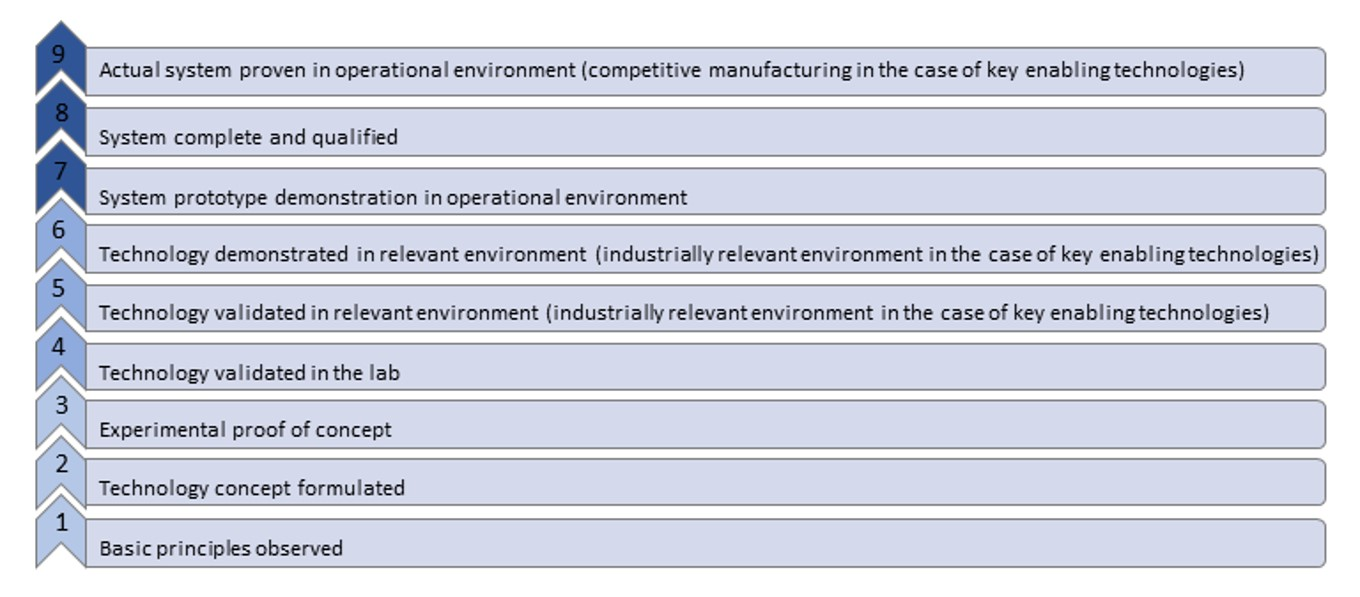
\includegraphics[width=0.9\linewidth]{image/TRL_cropped} \caption{Technology readiness scale}\label{fig:unnamed-chunk-4}
\end{figure}

Furthermore, we evaluate the readiness of a given technology to be acceptable in the society and how well it contributes to the public good using \textbf{societal readiness scale} (McCulloch, 2019):

\begin{figure}
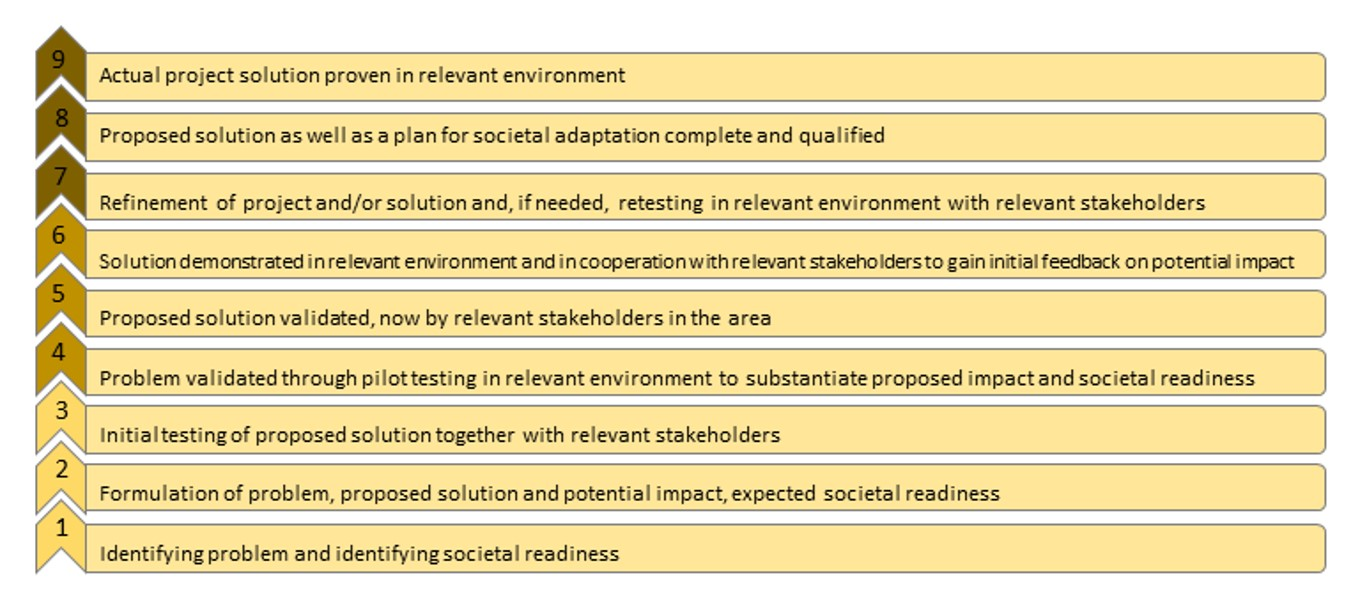
\includegraphics[width=0.9\linewidth]{image/SRL_cropped} \caption{Societal readiness scale}\label{fig:unnamed-chunk-5}
\end{figure}

Finally, we provide a list of \textbf{outstanding questions} and \textbf{links to additional sources} on the topic.

\textbf{References}

\begin{itemize}
\tightlist
\item
  Williamson, R., \& Beasley, J. (2011). \emph{Automotive technology and manufacturing readiness levels: a guide to recognised stages of development within the automotive industry}. URN11/672.
\item
  McCulloch, S. (2019). Social Acceptance And Societal Readiness Levels. \emph{DecarboN8}. Available at: \url{https://decarbon8.org.uk/social-acceptance-and-societal-readiness-levels/\#:~:text=Societal\%20readiness\%20refers\%20to\%20the,contributes\%20to\%20the\%20public\%20good.} {[}Accessed: 21 January 2021{]}.
\end{itemize}

\hypertarget{infrastructure}{%
\chapter{Physical road infrastructure}\label{infrastructure}}

\hypertarget{dedicated_lanes}{%
\section{Dedicated lanes for connected and automated vehicles (CAV)}\label{dedicated_lanes}}

\textbf{Updated: 14th February 2022}

\hypertarget{synonyms}{%
\subsection*{Synonyms}\label{synonyms}}
\addcontentsline{toc}{subsection}{Synonyms}

\emph{AV-dedicated lanes}, \emph{dedicated corridors}

\hypertarget{definition}{%
\subsection*{Definition}\label{definition}}
\addcontentsline{toc}{subsection}{Definition}

Dedicated lane for connected and autonomous vehicles features additional infrastructure or sensors to increase the reliability of \protect\hyperlink{adas}{Advanced Driver Assistant Systems (ADAS)}. Only automated driving vehicles are allowed to drive on these lanes. The typical applications include cooperative and adaptive cruise control based on sensors with the infrastructure, lane keeping, fuel use optimization and road pricing possibilities (Broek et al., 2011). The introduction of dedicated lanes for CAV is expected to have direct consequences on the traffic flow on the highways and a nearby road network. In particular, a study conducted in Singapore showed that dedicated lanes on the highways can reduce travel time of CAVs by approximately 25\% (if the saturation on the lane is not reached) at the cost of a delay for conventional cars of approximately 7\%, due to the reduced capacity (Ivanchev et al., 2017). They were also demonstrated to have a positive effect on fuel consumption.
Moreover, the throughput, defined as a number of vehicles passing through the road in a given time interval, increased as a result of introduction of dedicated lanes for AVs (Kumar et al., 2020). This effect, however, was associated with a decrease in throughput of smaller roads due to the preference of AVs for highways because of time savings, which in turn can result in time loss for conventional cars. What is more, the benefits from increased capacity of AV-only lanes can be further amplified through setting a higher speed limits for these lanes (Ye \& Yamamoto, 2018). With respect to the demand for different road types the study found that the introduction of dedicated CAV lanes will increase the demand of conventional cars for major road (but smaller than highways) and minor roads as a substitution for more congested highways due to the dedicated AV lanes.
In contrast, study by Chen et al.~(2016) showed that the implementation of CAV dedicated lanes has a potential of maximizing traffic capacity on these lanes in a mix-traffic context while having effectively no impact on conventional traffic capacity. Further, in order to use efficiently CAV dedicated lanes, which may be underutilized at the early stage, it is proposed to allow conventional cars to enter the AVs-only lanes after toll payment. This solution stems from currently operational across the world High Occupancy Vehicle (HOV) lanes. This joint approach is claimed to improve the throughput of individual road as well as enhance system-wide flow distribution within the network (Liu \& Song, 2019).

\hypertarget{key-stakeholders}{%
\subsection*{Key stakeholders}\label{key-stakeholders}}
\addcontentsline{toc}{subsection}{Key stakeholders}

\begin{itemize}
\tightlist
\item
  \textbf{Affected}: Conventional Cars' Drivers, Car Manufacturers, Insurers
\item
  \textbf{Responsible}: Road Infrastructure Agencies, Local and National Governments
\end{itemize}

\hypertarget{current-state-of-art-in-research}{%
\subsection*{Current state of art in research}\label{current-state-of-art-in-research}}
\addcontentsline{toc}{subsection}{Current state of art in research}

Current research focuses on gathering the evidence of the impact of the introduction of dedicated lanes on traffic flow, driver behaviour adoption, safety and efficiency. Furthermore, it analyses the factors which influence them, by testing different design and operation configurations, road types and utilization policies (Rad et al., 2020). Both, field operational testing and driving simulator studies have been conducted to investigate the influence of different designs of dedicated lanes on drivers in conventional cars and those featuring some degree of automation (Guin et al., 2008, Zhong, 2018). In particular, a number of studies compared distinct access types of dedicated lanes (Zhong, 2018, Yang et al., 2019). They showed that dedicated lanes with limited access performed better in terms of travel time and throughput compared to dedicated lanes with continuous access. Moreover, the probability of vehicles platooning was significantly higher on dedicated lanes with limited access. On the other hand, it was showed that collision rates near the entry or exit of these limited access lanes are higher (Rad et al.~2020).

Furthermore, the latest article by Fayyaz et al.~(2022) considers the impact of AV-dedicated lanes on urban space, mobility and development of sustainable cities. It discusses that the introduction of AVs could decrease overall parking demand in cities, leading to 10\% - 27\% release of urban space. With respect to traffic space, both the number and width of lanes might be reduced due to reduction in circulating vehicles (more shared AVs), platooning and the implementation of reversible lanes. On the other hand, some authors indicate that AVs have potential to decrease walking and cycling space by 26\% and 20\%, respectively. Similarly, study by Lee et al.~(2022) is concerned with street design strategies to implement AVs in large cities. The developed design allows for separation of AVs and regular vehicles through a connected zones allocated for AV usage.

Further, study by Ma et al.~(2022) proposes a shared-phase-dedicated-lane (SPDL)-based traffic control model at an isolated intersection with CAV dedicated lanes in the mixed traffic environment. The model aims at optimising the behaviour of vehicles and has been demonstrated to provide advantage in terms of average vehicle delay and intersection capacity.

\hypertarget{current-state-of-art-in-practice}{%
\subsection*{Current state of art in practice}\label{current-state-of-art-in-practice}}
\addcontentsline{toc}{subsection}{Current state of art in practice}

Currently state of Michigan together with several private partners including Ford and Alphabet Inc.~are planning to dedicate 65 km of a highway between Detroit and Ann Arbor for the sole movement of autonomous vehicles including buses and shuttles (Krisher \& Eggert, 2020). Similar initiatives are taking place in other countries, for instance, China set out to build nearly 100 km of 8-lane highway linking Beijing and the Xiongan New Area, from which 2 lanes will be allocated for the automated traffic. The completion of the construction phase is predicted by the end of 2020, while its opening is for traffic is expected in June 2021 (Syncedreview.com, 2020). In Europe, there is on-going SHOW (SHared automation Operating models for Worldwide adoption) project which aims to deploy about seventy automated vehicles in 21 European cities. To assess how they can best be integrated vehicles will be used in different settings in mixed traffic and dedicated lanes. However, for safety reasons the driver will be on-board (CORDIS, 2020).

\hypertarget{relevant-initiatives-in-austria}{%
\subsection*{Relevant initiatives in Austria}\label{relevant-initiatives-in-austria}}
\addcontentsline{toc}{subsection}{Relevant initiatives in Austria}

\begin{itemize}
\tightlist
\item
  \href{https://www.tugraz.at/fileadmin/user_upload/Institute/IHF/Projekte/ENABLE-S3_SummaryofResults_May2019.pdf}{tugraz.at}
\item
  \href{https://www.ait.ac.at/themen/verkehrssicherheit-und-unfallforschung/projects/via-autonom/}{ait.ac.at}
\end{itemize}

\hypertarget{impacts-with-respect-to-sustainable-development-goals-sdgs}{%
\subsection*{Impacts with respect to Sustainable Development Goals (SDGs)}\label{impacts-with-respect-to-sustainable-development-goals-sdgs}}
\addcontentsline{toc}{subsection}{Impacts with respect to Sustainable Development Goals (SDGs)}

\begin{longtable}[]{@{}
  >{\centering\arraybackslash}p{(\columnwidth - 8\tabcolsep) * \real{0.2029}}
  >{\centering\arraybackslash}p{(\columnwidth - 8\tabcolsep) * \real{0.1884}}
  >{\centering\arraybackslash}p{(\columnwidth - 8\tabcolsep) * \real{0.2029}}
  >{\centering\arraybackslash}p{(\columnwidth - 8\tabcolsep) * \real{0.2029}}
  >{\centering\arraybackslash}p{(\columnwidth - 8\tabcolsep) * \real{0.2029}}@{}}
\toprule()
\begin{minipage}[b]{\linewidth}\centering
Impact level
\end{minipage} & \begin{minipage}[b]{\linewidth}\centering
Indicator
\end{minipage} & \begin{minipage}[b]{\linewidth}\centering
Impact direction
\end{minipage} & \begin{minipage}[b]{\linewidth}\centering
Goal description and number
\end{minipage} & \begin{minipage}[b]{\linewidth}\centering
Source
\end{minipage} \\
\midrule()
\endhead
Individual & Fuel consumption reduced & \textbf{+} & Environmental sustainability (\emph{7,12,13,15}) & Ivanchev et al., 2017 \\
Individual & Travel time reduced & \textbf{+} & Sustainable economic development (\emph{8,11}) & Zhong, 2018; Yang et al., 2019 \\
Systemic & Collision rate reduced & \textbf{+} & Health \& Wellbeing (\emph{3}) & Zhang et al., 2020 \\
Systemic & Emissions rate reduced & \textbf{+} & Environmental sustainability (\emph{7,12,13,15}) & Al Alam at al., 2010 \\
Systemic & Congestion & \textbf{\textasciitilde{}} & Sustainable economic development (\emph{8,11}) & Ivanchev et al., 2017; Kumar et al., 2020 \\
Systemic & Novel designs tested & \textbf{+} & Innovation \& Infrastructure (\emph{9}) & Guin et al., 2008; Zhong, 2018; Krisher \& Eggert, 2020 \\
Systemic & SHOW EU initiative & \textbf{+} & Partnership \& collaborations (\emph{17}) & CORDIS, 2020 \\
\bottomrule()
\end{longtable}

\hypertarget{technology-and-societal-readiness-level}{%
\subsection*{Technology and societal readiness level}\label{technology-and-societal-readiness-level}}
\addcontentsline{toc}{subsection}{Technology and societal readiness level}

\begin{longtable}[]{@{}cc@{}}
\toprule()
TRL & SRL \\
\midrule()
\endhead
5-6 & 1-3 \\
\bottomrule()
\end{longtable}

\hypertarget{open-questions}{%
\subsection*{Open questions}\label{open-questions}}
\addcontentsline{toc}{subsection}{Open questions}

\begin{enumerate}
\def\labelenumi{\arabic{enumi}.}
\tightlist
\item
  What are the potential benefits of dedicated AV lanes when coupled with smart platooning strategies?
\item
  How and to what degree will joint concepts by automotive sector, fleet and road
  operators will improve traffic management establishing dynamic traffic regulations even across
  borders?
\item
  What are the roles and responsibilities of the different stakeholders of physical infrastructure for connected and automated vehicles?
\item
  Should the vehicle cope with any road infrastructure, and if not, what demands can be set to adapt the existing infrastructure?
\item
  How to ensure continuity between those different environments?
\item
  Which tools (e.g.~micro- and macroscopic transport modelling, impact assessment) can enable
  cities to assess the impact of automated vehicles on their physical road infrastructure and
  balance the needs of automated vehicles against the needs of existing modes (conventional
  vehicles, public transport, pedestrians and cyclists). (ERTRAC, 2019)
\item
  Does the implementation of AVs support or hinder the concept of driverless cities?
\end{enumerate}

\hypertarget{further-links}{%
\subsection*{Further links}\label{further-links}}
\addcontentsline{toc}{subsection}{Further links}

\begin{itemize}
\tightlist
\item
  \href{https://knowledge-base.connectedautomateddriving.eu/wp-content/uploads/2019/12/SMART_2010-0064-study-report-final_V1-2.pdf}{Knowledge base}
\item
  \href{https://show-project.eu/}{SHOW project}
\item
  \href{https://www.automotiveworld.com/articles/autonomous-only-should-avs-have-dedicated-lanes/}{Automotive world}
\end{itemize}

\hypertarget{references}{%
\subsection*{References}\label{references}}
\addcontentsline{toc}{subsection}{References}

\begin{itemize}
\tightlist
\item
  Al Alam, A., Gattami, A., \& Johansson, K. H. (2010, September). An experimental study on the fuel reduction potential of heavy duty vehicle platooning. In 13th International IEEE Conference on Intelligent Transportation Systems (pp.~306-311). IEEE.
\item
  Broek, S. M., van Nunen, E., \& Zwijnenberg, H. (2011). Definition of necessary vehicle and infrastructure systems for automated driving.
\item
  Chen, Z., He, F., Zhang, L., \& Yin, Y. (2016). Optimal deployment of autonomous vehicle lanes with endogenous market penetration. Transportation Research Part C: Emerging Technologies, 72, 143-156.
\item
  CORDIS \textbar{} European Commission. (20 Apr 2020). Available at: \url{https://cordis.europa.eu/project/id/875530} {[}Accessed: 13 November 2020{]}.
\item
  ERTRAC Working Group. (2019). Connected Automated Driving Roadmap. version, 8, 2019-08.
\item
  Fayyaz, M., González-González, E., \& Nogués, S. (2022). Autonomous Mobility: A Potential Opportunity to Reclaim Public Spaces for People. Sustainability, 14(3), 1568.
\item
  Guin, A., Hunter, M., \& Guensler, R. (2008). Analysis of reduction in effective capacities of high-occupancy vehicle lanes related to traffic behavior. Transportation Research Record, 2065(1), 47-53.
\item
  Ivanchev, J., Knoll, A., Zehe, D., Nair, S., \& Eckhoff, D. (2017). Potentials and implications of dedicated highway lanes for autonomous vehicles. arXiv preprint arXiv:1709.07658.
\item
  Krisher, T., \& Eggert, D. (14 Aug 2020). Michigan plans dedicated road lanes for autonomous vehicles. Available at: \url{https://abcnews.go.com/Technology/wireStory/michigan-plans-dedicated-road-lanes-autonomous-vehicles-72352758} {[}Accessed: 12 November 2020{]}.
\item
  Kumar, A., Guhathakurta, S., \& Venkatachalam, S. (2020). When and where should there be dedicated lanes under mixed traffic of automated and human-driven vehicles for system-level benefits?. Research in Transportation Business \& Management, 100527.
\item
  Lee, S., Jang, K. M., Kang, N., Kim, J., Oh, M., \& Kim, Y. (2022). Redesigning urban elements and structures considering autonomous vehicles: Preparing design strategies for wide implementation in cities. Cities, 123, 103595.
\item
  Liu, Z., \& Song, Z. (2019). Strategic planning of dedicated autonomous vehicle lanes and autonomous vehicle/toll lanes in transportation networks. Transportation Research Part C: Emerging Technologies, 106, 381-403.
\item
  Ma, W., Li, J., \& Yu, C. (2022). Shared-phase-dedicated-lane based intersection control with mixed traffic of human-driven vehicles and connected and automated vehicles. Transportation Research Part C: Emerging Technologies, 135, 103509.
\item
  Rad, S. R., Farah, H., Taale, H., van Arem, B., \& Hoogendoorn, S. P. (2020). Design and operation of dedicated lanes for connected and automated vehicles on motorways: A conceptual framework and research agenda. Transportation Research Part C: Emerging Technologies, 117, 102664.
\item
  Syncedreview.com (31 Aug 2020). Beijing Builds 100km Highway Lanes for Self-Driving Cars with Unmanned Machineries. Available at: \url{https://syncedreview.com/2020/08/31/beijing-builds-100km-highway-lanes-for-self-driving-cars-with-unmanned-machineries/} {[}Accessed: 12 November 2020{]}.
\item
  Yang, D., Farah, H., Schoenmakers, M. J., \& Alkim, T. (2019). Human drivers behavioural adaptation when driving next to a platoon of automated vehicles on a dedicated lane and implications on traffic flow: a driving simulator and microscopic simulation study in the Netherlands. In 98th Annual Meeting of the Transportation Research Board (pp.~19-00582).
\item
  Ye, L., \& Yamamoto, T. (2018). Impact of dedicated lanes for connected and autonomous vehicle on traffic flow throughput. Physica A: Statistical Mechanics and its Applications, 512, 588-597.
\item
  Zhang, J., Wu, K., Cheng, M., Yang, M., Cheng, Y., \& Li, S. (2020). Safety Evaluation for Connected and Autonomous Vehicles' Exclusive Lanes considering Penetrate Ratios and Impact of Trucks Using Surrogate Safety Measures. Journal of advanced transportation, 2020.
\item
  Zhong, Z. (2018). Assessing the effectiveness of managed lane strategies for the rapid deployment of cooperative adaptive cruise control technology.
\end{itemize}

\hypertarget{ODD}{%
\section{Operational design domains}\label{ODD}}

\hypertarget{synonyms-1}{%
\subsection*{Synonyms}\label{synonyms-1}}
\addcontentsline{toc}{subsection}{Synonyms}

\emph{ODD}

\hypertarget{definition-1}{%
\subsection*{Definition}\label{definition-1}}
\addcontentsline{toc}{subsection}{Definition}

Operational design domain is a system to assess the conditions in which automated driving system (ADS) is designed to work safely based on roadway features or amount of traffic (Czarnecki, 2018). It is a key to the safety of automated vehicles and ODD is in place to define the limitations for driving at different automation level of a vehicle (Eliot, 2019). For example, level 5 automation has an unconstrained ODD which means that it is equivalent of human driver controlling the vehicle. In terms of levels 1-4 the ODD puts constraints with respect to (Czarnecki, 2018):

\begin{itemize}
\tightlist
\item
  Road environment: including but not limited to urban and rural roads, motorways, roundabouts, tunnels, traffic volumes, construction areas, or different weather or visibility conditions
\item
  State of the vehicle: for instance, load limits or minimum tire inflation level
\item
  Behaviour of the vehicle equipped with ADS: for example, speed limits or constraints on possible manoeuvres
\end{itemize}

In general, ODD assesses if the conditions are appropriate for a vehicle to drive autonomously on the chosen route and given automation level. If at some stage ODD finds that conditions are not appropriate for autonomous driving, it will find a spot to stop the vehicle and the driver will be required to take over and start driving by himself.

The ODD works based on the operational world model (OWM) that consist of \emph{operational road environment model (OREM)}, \emph{the subject vehicle(s) model (SVM)} and \emph{subject ADS}. OREM represents all the relevant assumptions about the road environment in which an ADS will operate, while ignoring the irrelevant ones. SVM represents a vehicle operated by the developed ADS. The OMW may include single subject vehicle or multiple subject vehicles equipped with the same or different ADS. Inclusion of distinct ADSs may be necessary to represent the interaction between different types of vehicles such as buses and passenger vehicles or the same types of vehicles under different ADS development level.

Further, Koopman and Fratrik (2019) provide list of factors which are found to be relevant for the validation and operation of automated vehicles and consequently for the development of ODD. These include:

\begin{itemize}
\tightlist
\item
  Operational terrain
\item
  Weather conditions
\item
  Operational infrastructure
\item
  Rules of engagement and interaction with environment and other road other users
\item
  Considerations for deployment to multiple regions
\item
  Data availability and recency (e.g.~Regarding temporary changes in traffic rules)
\item
  Expected elements of operational space state (e.g.~What should be included in the scope of ODD)
\end{itemize}

Moreover, Object and Event Detection and Response (OEDR) refers to the operation within the scope of a defined ODD with respect to objects and events. \emph{Object factors} include:

\begin{itemize}
\tightlist
\item
  Ability to detect and classify relevant objects in the environment
\item
  Processing and thresholding of sensors data
\item
  Characterising possible operational parameters of other road users
\item
  Permanent (Trees, curbs etc.) and temporary (e.g.~People, floods) obstacles
\item
  At risk population
\item
  All types of other road users including human-driven and autonomous vehicles as well as special purpose vehicles and aircrafts
\end{itemize}

Moreover, the \emph{Events factors} refer to:

\begin{itemize}
\tightlist
\item
  Determination of behaviour of other objects
\item
  `Normal' movement of objects
\item
  `Abnormal' movement of objects
\item
  Failure to move of other objects
\item
  Drivers' interactions before, during and after the autonomous system engagement
\item
  Human and non-human interactions
\end{itemize}

\hypertarget{key-stakeholders-1}{%
\subsection*{Key stakeholders}\label{key-stakeholders-1}}
\addcontentsline{toc}{subsection}{Key stakeholders}

\begin{itemize}
\tightlist
\item
  \textbf{Affected}: Conventional Cars' Drivers, Car Manufacturers, Users of AVs
\item
  \textbf{Responsible}: Council authorities, Car manufacturers, Insurance providers
\end{itemize}

\hypertarget{current-state-of-art-in-research-1}{%
\subsection*{Current state of art in research}\label{current-state-of-art-in-research-1}}
\addcontentsline{toc}{subsection}{Current state of art in research}

Current research focuses on the validation, extension of capabilities and an improvement in accuracy of current ODD systems. For example, Lee et al.~(2020) proposes an approach to identify an ODD for the ADS using statistical data and risk tolerance. The identified ODD is based on the geographical mapping of risk level associated with ADS operation that is below the risk threshold predefined for a given environmental conditions. Therefore, this method allows for addressing safety concerns through the provision of geographical and environmental constrains to ADS operation. Further, Farah et al.~(2020) looked at understanding of ODD (with respect to lane keeping) by human drivers, where they are expected to control the vehicle in situation outside of ODD specified by the manufacturer. A difference between driver's understanding of the AV's capabilities and manufacturers manual can lead to severe safety issues. They conducted a field test using Tesla Model S based on the situation within and beyond ODD specified by the manufacturer. Farah et al.~(2020) found a mismatch between manufacturer's specified ODD and driver's perception of what ODD includes. In particular, often situation out of scope of the ODD were classified by the human driver as that within ODD domain. This study demonstrated the need for clearer description and specification of ODD to diminish the discrepancy between driver's awareness and actual vehicle abilities.

\hypertarget{current-state-of-art-in-practice-1}{%
\subsection*{Current state of art in practice}\label{current-state-of-art-in-practice-1}}
\addcontentsline{toc}{subsection}{Current state of art in practice}

California is one of the pioneering states that makes attempts at testing of ODD. One of the examples is current Google's project of \href{https://www.losaltoshills.ca.gov/DocumentCenter/View/2315/Waymo_Driverless_Autonomous_Vehicle_Tester_Program}{Waymo's} driverless testing car. It uses a 4th stage of automated driving system and shows the usage of ODD in real life. Waymo's ODD works on the certain geographic area (part of California) 24 hours a day. Waymo's ODD allows reach up to 105 km/h, however it does not operate when is snowy or rainy. Otherwise, in the USA there is not any nationwide policy regarding use of ODD because these are highly location-specific. Other world regions are working their own regulation with respect to ODDs such as MLIT-Guidline in Japan, Transport Canada in Canada, NHTSA FAVP 3.0 in the USA or EC Guidelines in Europe. Furthermore, the UN Informal Working Group on Functional Requirements for AVs (FRAV) put forward a \href{https://unece.org/fileadmin/DAM/trans/doc/2020/wp29grva/GRVA-05-40e.pdf}{report} to regulate the functional performance requirements for Automated Driving Systems and vehicles equipped with such systems.

\hypertarget{relevant-initiatives-in-austria-1}{%
\subsection*{Relevant initiatives in Austria}\label{relevant-initiatives-in-austria-1}}
\addcontentsline{toc}{subsection}{Relevant initiatives in Austria}

\begin{itemize}
\tightlist
\item
  \href{https://austriatech.at/de/das-konzept-der-isad-klassen/}{AustriaTech}
\end{itemize}

\hypertarget{impacts-with-respect-to-sustainable-development-goals-sdgs-1}{%
\subsection*{Impacts with respect to Sustainable Development Goals (SDGs)}\label{impacts-with-respect-to-sustainable-development-goals-sdgs-1}}
\addcontentsline{toc}{subsection}{Impacts with respect to Sustainable Development Goals (SDGs)}

\begin{longtable}[]{@{}
  >{\centering\arraybackslash}p{(\columnwidth - 8\tabcolsep) * \real{0.2029}}
  >{\centering\arraybackslash}p{(\columnwidth - 8\tabcolsep) * \real{0.1884}}
  >{\centering\arraybackslash}p{(\columnwidth - 8\tabcolsep) * \real{0.2029}}
  >{\centering\arraybackslash}p{(\columnwidth - 8\tabcolsep) * \real{0.2029}}
  >{\centering\arraybackslash}p{(\columnwidth - 8\tabcolsep) * \real{0.2029}}@{}}
\toprule()
\begin{minipage}[b]{\linewidth}\centering
Impact level
\end{minipage} & \begin{minipage}[b]{\linewidth}\centering
Indicator
\end{minipage} & \begin{minipage}[b]{\linewidth}\centering
Impact direction
\end{minipage} & \begin{minipage}[b]{\linewidth}\centering
Goal description and number
\end{minipage} & \begin{minipage}[b]{\linewidth}\centering
Source
\end{minipage} \\
\midrule()
\endhead
Systemic & Aim at increasing safety in autonomous cars & \textbf{+} & Health \& Wellbeing (\emph{3}) & Koopman and Fratrik, 2019 \\
Systemic & Developing fully autonomous cars & \textbf{+} & Innovation \& Infrastructure (\emph{9}) & Waymo, 2019 \\
\bottomrule()
\end{longtable}

\hypertarget{technology-and-societal-readiness-level-1}{%
\subsection*{Technology and societal readiness level}\label{technology-and-societal-readiness-level-1}}
\addcontentsline{toc}{subsection}{Technology and societal readiness level}

\begin{longtable}[]{@{}cc@{}}
\toprule()
TRL & SRL \\
\midrule()
\endhead
5-6 & 4-6 \\
\bottomrule()
\end{longtable}

\hypertarget{open-questions-1}{%
\subsection*{Open questions}\label{open-questions-1}}
\addcontentsline{toc}{subsection}{Open questions}

\begin{enumerate}
\def\labelenumi{\arabic{enumi}.}
\tightlist
\item
  How does the development of ODD influence the autonomous cars market toward to the average driver?
\end{enumerate}

\hypertarget{references-1}{%
\subsection*{References}\label{references-1}}
\addcontentsline{toc}{subsection}{References}

\begin{itemize}
\tightlist
\item
  Berman, B., 2019. Autonomous vehicle operation design domain is key to safety. Sae.org. Available at: \url{https://www.sae.org/news/2019/11/odds-for-av-testing} {[}Accessed: 2 August 2021{]}.
\item
  Czarnecki, K. (2018). Operational Design Domain for Automated Driving Systems - Taxonomy of Basic Terms. 10.13140/RG.2.2.18037.88803.
\item
  Eliot, L., 2019. Key To Driverless Cars, Operational Design Domains (ODD), Here's What They Are, Woes Too. Medium. Available at: \url{https://lance-eliot.medium.com/key-to-driverless-cars-operational-design-domains-odd-heres-what-they-are-woes-too-a0f1059e0bdb} {[}Accessed: 2 August 2021{]}.
\item
  Farah, H., Bhusari, S., Van Gent, P., Babu, F. A. M., Morsink, P., Happee, R., \& van Arem, B. (2020). An empirical analysis to assess the operational design domain of lane keeping system equipped vehicles combining objective and subjective risk measures. IEEE Transactions on Intelligent Transportation Systems, 22(5), 2589-2598.
\item
  Koopman, P. and Fratrik, F., (2019). How Many Operational Design Domains, Objects, and Events?. Ceur-ws.org. Available at: \url{http://ceur-ws.org/Vol-2301/paper_6.pdf} {[}Accessed: 2 August 2021{]}.
\item
  Law Insider. (2021). Operational design domain Definition \textbar{} Law Insider. Available at: \url{https://www.lawinsider.com/dictionary/operational-design-domain} {[}Accessed: 2 August 2021{]}.
\item
  Lee, C., Nayeer, N., Garcia, D., Agrawal, A. and Liu, B., 2020. Identifying the Operational Design Domain for an Automated Driving System through Assessed Risk. 2020 IEEE Intelligent Vehicles Symposium (IV).
\item
  Waymo. 2019. Waymo. Available at: \url{https://waymo.com/} {[}Accessed: 2 August 2021{]}.
\end{itemize}

\hypertarget{rail_crossing_info_system}{%
\section{Rail crossing information system}\label{rail_crossing_info_system}}

\hypertarget{synonyms-2}{%
\subsection*{Synonyms}\label{synonyms-2}}
\addcontentsline{toc}{subsection}{Synonyms}

\emph{rail level crossings (RLX), raised level crossings (RC), Level Crossing Obstacle Detection (LOD), level crossing (LC)}

\hypertarget{definition-2}{%
\subsection*{Definition}\label{definition-2}}
\addcontentsline{toc}{subsection}{Definition}

A persistent problem in surface transportation are the collisions at rail level crossings (RLX). RLX are grade-separated crossings where rail vehicles (and their infrastructure) cross the infrastructure of another mode of transport (usually roads). In most cases, the train has priority and other traffic is stopped until the train has passed. Technically, achieving this unbundling is a simple problem (Salmon et al., 2016). Nevertheless, a number of accidents still happen every year.

Collisions at level crossings are a safety risk worldwide (European Railway Agency, 2020). Accidents cause human, social and economic costs. In addition, near-collisions have a negative impact on the mental health and well-being of the people involved - car drivers, train drivers and bystanders (Read et al., 2021). The best way to minimise these types of accidents would be to eliminate the level crossings and/or replace them with tunnels or bridges. As these options are very expensive, the cheaper alternative of signage, flashing lights and barriers is used for most level crossings, in the expectation that drivers of road vehicles will obey the rules. However, data from Australia shows that the largest proportion of collisions are at barrier intersections, while the largest proportion of fatal accidents are at flashing light and stop sign intersections (ITSR, 2011).

Radalj et al.~(2011) have demonstrated, through an extensive field study in seven rural LCs, that 90\% of the road users disobeyed the speed limits on the signals and that 90\% of the crashes at railway level crossings could be attributed to vehicle driver errors, fatigue, speed or risk taking due to low frequency of trains. In Austria, too, there is already data indicating that practically all accidents at level crossings are caused by road users who do not respect red lights, stop signs, barriers and basic traffic rules. Very often, people who live near a railway crossing or cross it regularly are involved in these accidents because they become more careless and overconfident over time (bmvit, 2011).

According to European Union (2014), level crossings are divided into active and passive:

\begin{itemize}
\tightlist
\item
  \textbf{Passive level crossing} is a level crossing without any form of warning system or protection that is activated when it is unsafe for the user to cross
\item
  \textbf{Active level crossing} is a level crossing where the users of the level crossing are protected or warned against the approaching train. Protection is provided by half or full barriers. The warning is given by the use of visible devices (e.g.~lights) and acoustic devices (e.g.~bells, horns, sound signals).
\end{itemize}

Active level crossings are classified as:

\begin{itemize}
\tightlist
\item
  \textbf{Manual}: a level crossing where the user-side protection or warning is activated manually by a railway employee.
\item
  \textbf{Automatic with user-side warning}: a level crossing where the user-side warning is activated by the approaching train.
\item
  \textbf{Automatic with user-side protection}: a level crossing where the user-side protection is activated by the approaching train. This includes a level crossing that has both user-side protection and a warning.
\item
  \textbf{Track-side protection}: a level crossing where a signal or other train protection system allows a train to proceed only if the level crossing is clear of obstructions.
\end{itemize}

Trackside protection enables obstacle detection at level crossings by one or more detection units, depending on the size of the level crossing. A track side control unit collects the information received from the detection units and generates alarms based on high thresholds (e.g.~minimum dimensions of the obstacle). The control unit is able to integrate the level crossing obstacle detection (LOD) into the conventional level crossing protection system with complete barriers and drives and to communicate with the interlocking system via secured interfaces. The systems are characterised by high reliability and high accuracy, even in harsh weather conditions such as rain, snow and fog. Several trials are currently underway with European railways (mermecgroup, n.d.).

According to Darlington (2017) an ideal obstacle detection system must:

\begin{itemize}
\tightlist
\item
  provide safety integrity that is no worse and ideally better than a manually operated level crossing
\item
  cause no or minimal delays to trains due to equipment failures or false detections
\item
  be affordable in terms of life cycle costs
\item
  operate in all weather conditions and temperatures
\item
  be practical to use and maintain
\end{itemize}

Beyond, separate technology systems must confirm that the level crossing is closed by barriers or gates, and only when the detection system has reconfirmed that the level crossing is clear, the train is allowed to pass. This could be achieved by clearing the protection signals or, on some rail networks, by a direct communication link to the train. Some systems may offer good safety benefits, but only at the cost of significant operational delays. The obstacle detection system must also fit into the existing railway infrastructure and not interfere with rolling stock or operations.

The following technologies are available for obstacle detection , however, all have advantages and disadvantages (Darlington, 2017):

\textbf{Video imaging technology}
The disadvantage of using video technology is that it is more difficult for the system to detect anything at night or in fog. The level crossing may therefore need the same or higher illuminance than a manual level crossing, although even this would be of little help in foggy conditions. Furthermore, the mass or material properties of an object may not be so easily distinguished. Therefore, a cardboard box or newspaper, for example, could be mistaken for a small child.

\textbf{Thermal imaging}
Thermal imaging cameras can overcome some of these limitations because they produce a sharp image based on subtle temperature differences and are not affected by environmental conditions such as total darkness, smoke or fog. They do not require any light and cannot be blinded by direct sunlight. However, objects without a heat source could be left at an intersection (for example, an unbraked trailer) and thus not be detected. Thermal imaging, in combination with other detection technologies, can provide a solution.

\textbf{Millimetre wavelength beam interruption}
Beam interruption is an obstacle detection technique based on microwaves. When an object enters the beam path, the signal to the transceiver is attenuated, indicating its presence. One of the world's first Safety Integrity Level (SIL) 4 systems was installed in Italy. Although the system was safe, it was very sensitive to temperature changes, rain and condensation on the transmitter and receiver sensors. Regular calibration and maintenance had to be carried out. Furthermore, the narrow beam width and limited field of view meant that even more sensors were needed for tall objects.

\textbf{LiDAR}
LiDAR detects the crossing area with pulses of near-infrared light that are reflected from the surface of an object on the level crossing. The reflected pulses can then be analysed to determine its position, direction and speed. Because light has shorter wavelengths than radio waves, LiDAR has the potential for greater accuracy than radar. Network Rail used LiDAR on its first generation of OD crossings as a complement to radar to improve low-level object detection. However, the improved sensitivity also means it is vulnerable to small objects, such as water vapour droplets that make up fog, although this can be mitigated by software algorithms. Furthermore, light is required for operation and the devices must be housed in a transparent enclosure resulting in increased susceptibility to water, dirt and dust on the glass.

\textbf{Induction loops}
An induction loop is used to detect metal objects, so is not suitable for pedestrian detection. Unfortunately, there are an increasing number of road vehicles made of composite materials and aluminium, which provide a lower induced current than steel, and problems have been reported in detecting trucks with high axles/ground clearance. Another difficulty is the installation and maintenance of induction loops in the surface of the crossing or road.

\textbf{Strain gauges}
A strain gauge or piezometer can be used to measure the deformation (strain) of a material (the deformation of the crossing surface when an object crosses the level crossing). A strain gauge should be able to be calibrated for both vehicles and pedestrians, but may not be able to detect small children. Piezometers and strain gauges have the potential to be more reliable than inductive loops, but the placement of the detectors in the crossing pavement makes them just as difficult to maintain.

\textbf{Ultrasonic sensors}
These emit ultrasonic sound pulses that cannot be detected by the human ear. When the pulse reaches an object, the sound is reflected off the surface. Multiple sensors would be required to avoid black spots, and on electrified lines the devices would be in close proximity to parts of the overhead lines. The devices would be more susceptible to vandalism and damage by the public as they are much more conspicuous at a level crossing than other forms of detection. However, it is reported that successful obstacle detection trials have been carried out in the USA using an array of ultrasonic sensors suspended above a level crossing.

\textbf{Radar}
This uses radio waves to detect objects. The distance, position and speed of an object can be determined. Reflectors can be installed at the boundaries of the level crossing to provide a reference echo signal and use this to monitor the condition of the area and the sensor itself. Radar-based systems are able to reliably detect objects through rain, fog, snow and hail. OD radar systems with SIL 4 integrity have been developed and systems with a wide beam width so that multiple sensors are not required for high and low obstacles. An advantage of radar over other detection methods is that some low-density material objects, such as an empty paper box, are ignored. As it is a radio-based system, a radar OD system normally requires a radio licence, but this means that the railway infrastructure manager has exclusive use of the frequency and is able to manage any interference. The sensor is capable of operating in all weather conditions and has a predicted Mean Time Between Failures MTBF of more than 10 years.

An OD system may use one or more of the different detection types, e.g.~Network Rail's first-generation OD crossings use both radar and Laser Image Detection and Ranging (LiDAR).

\hypertarget{key-stakeholders-2}{%
\subsection*{Key stakeholders}\label{key-stakeholders-2}}
\addcontentsline{toc}{subsection}{Key stakeholders}

\begin{itemize}
\tightlist
\item
  \textbf{Affected}: Drivers, Cyclists, Pedestrians, Train Passengers, Train Operators, Train Drivers
\item
  \textbf{Responsible}: National Governments, City Governments, Transport Agencies, Railway companies, Rail Equipment and Infrastructure Producers and Manufacturers
\end{itemize}

\hypertarget{current-state-of-art-in-research-2}{%
\subsection*{Current state of art in research}\label{current-state-of-art-in-research-2}}
\addcontentsline{toc}{subsection}{Current state of art in research}

A driving simulation study (Larue et al., 2015) showed that driver behaviour changed with assistive ITS interventions at passive crossings, while no differences were observed at active crossings, even with limited visibility. The audio intervention resulted in higher compliance compared to the visual intervention. The results of road-based ITS technology suggest that this is unlikely to lead to positive safety outcomes at passive level crossings if drivers are still required to stop at the level crossing under all conditions (due to the stop sign at the level crossing). In-vehicle audio intervention is most likely to provide safety benefits because humans are able to hear sound regardless of the direction from which the sound is coming. This makes sound a particularly useful medium for the transmission of safety-critical messages.

Many authors investigate driver behaviour at railway crossings (Beanland et al., 2017; Hao et al., 2015; Larue et al., 2015; Tey et al., 2013). A systematic study by Read et al.~(2021) categorises factors that influence risk at rail level crossings according to 3 issues:

\begin{itemize}
\tightlist
\item
  accident rate and severity
\item
  unsafe and non-compliant road user behaviour
\item
  road user risk perceptions, attitudes and beliefs
\end{itemize}

Most studies focused on unsafe and/or non-compliant road user behaviour.

Results from Beanland et al.~(2017) suggest that while significant slowing at passive RLXs is necessary to give drivers time to visually check for trains, stop signs are not necessary as drivers who stopped rolling and those who stopped fully spent equal amounts of time visually checking for trains and showed similar situational awareness. Similarly, a full stop is problematic for some vehicles (e.g.~heavy vehicles that lose momentum and require more time and energy to regain speed). Years ago, some researchers have also argued against the use of stop signs at RLXs, fearing that the high rates of observed non-compliance will generalise this behaviour and lead to non-compliance at stop-controlled highway and road intersections (Austin \& Carson, 2002; Raub, 2009). Zhang et al.~(2019) investigated raised level crossings (RC) as an alternative to the current form of level crossings to mitigate the severity of accidents at road-rail crossings. Further, Larue et al.~(2015) categorized 3 ITS applications for railway crossings:

\begin{itemize}
\tightlist
\item
  \textbf{In-vehicle visual system}: A warning system with GPS (as a smartphone application). In particular, such a system should improve the driver's awareness of the crossing condition while approaching a crossing with limited visibility (curves, gradients, fog or sun glare).
\item
  \textbf{In-vehicle audio warning (radio interference)}: When a train approached the level crossing, the loudspeakers gave a verbal warning while the flashing lights of active level crossings were activated. For passive crossings, the warning was given 20 s before the train arrived.
\item
  \textbf{Roadside flashing ITS beacons}: This road-based ITS used flashing warning beacons on the road. They were activated when a train approached the level crossing. These beacons marked the place where the driver should stop his vehicle, similar to illuminated runways of aeroplanes. This system was intended to increase the visibility of the crossing status at all times of the day, leading drivers to notice the crossing status earlier, even when visibility was limited (no further information could be found, about which systems are still in development and at which status).
\end{itemize}

Fayyaz \& Johnson (2020) suggest to use deep learning technology in radar and video monitoring systems to better classify objects or locate their exact position in the given frame, as the environment of level crossings is dynamic (growing vegetation and frequently harmless objects). Thus, the technology is not intended to rely on raw pixel values, but rather on the features and actual representation of the object.

\hypertarget{current-state-of-art-in-practice-2}{%
\subsection*{Current state of art in practice}\label{current-state-of-art-in-practice-2}}
\addcontentsline{toc}{subsection}{Current state of art in practice}

According to the European Railway Agency (2020) safety at level crossings has improved over the last ten years. With 1,721 significant accidents, the lowest number since 2010 was recorded in 2018. The decrease is mainly due to `external' accidents involving third parties (unauthorised persons and level crossing users). Between 2006 and 2018, rail fatalities decreased by 60\% (an average of 4.6\% p.a.). Level crossing accidents and fatalities account for more than a quarter of all rail accidents on EU railways. Every year, almost 300 people die in LC accidents (EU-28), with an estimated economic loss of €1 billion.

There are about 105 000 level crossings in the EU-28 countries. Passive level crossings account for 49\% of all level crossings. These level crossings are usually equipped with a St Andrew's cross but do not provide active warning to road users. Level crossings with user protection (arm barriers and flashing lights) are the most common type of active level crossing (45 \%). Level crossings combining full roadside protection with rail protection account for 16 \% (17 277) of all level crossings. Passive level crossings and level crossings in general are disappearing at a slow pace. If the current trend continues, there will still be around 35 000 level crossings on the EU rail network by the end of the century, of which 5 000 will be passive. The last report assessing the achievement of the safety targets showed acceptable safety performance in all Member States in the categories of passengers, level crossing users and societal risks. For the category of level crossing users, it was the first time since the 2013 assessment that no country showed a possible deterioration (European Railway Agency, 2019). Network Rail (2019) has set the following priorities for level crossing information systems:

\begin{itemize}
\tightlist
\item
  Unsecured automatic level crossings - the automatic half-barrier crossing.
\item
  Automatic level crossings that inform the driver whether the level crossing is clear before a train can pass the crossing.
\item
  Improvement and installation of visual and acoustic warnings
\end{itemize}

To further improve safety at level crossings, obstacle detection systems are used at level crossings. Systems are classified into a safety integrity level (SIL), which has a four-level scale, with SIL 1 being the minimum safety requirement and SIL 4 being the most stringent. These levels are used to specify the safety integrity requirements for the safety functions performed by safety systems (Gabriel et al., 2018).

Traditional (intrusive) sensors installed on or in the railway tracks (e.g.~inductive loops and strain gauges) interfere with the rail tracks during their installation and maintenance, making the system costly and unsuitable for its applicability at level crossings. Non-intrusive sensors (e.g.~radar and CCTV) are installed outside the tracks and do not disturb the tracks during installation and maintenance periods. The low cost and long product life cycle of these sensors make radar and CCTV the preferred choice for level crossing applications (Fayyaz \& Johnson, 2020).

The L.B. Foster company in the US already has several LODs in use for red light violation monitoring, number plate recognition, video analysis and data recording. The red light violation camera system has led to thousands of prosecutions for dangerous driving. The requirement to detect a 9-year-old child while lying on the level crossing proved challenging. This meant detecting any object with a size of 115mm height. The technology chosen to meet this specification was a LIDAR detector, which after 3 months of ground testing proved that it was possible to detect an object of this size after modifications. Integrating the system into typical signalling circuits also proved challenging as there were many relay circuits to consider, not only for obstacle detection but for all fault modes etc (Roberts, 2018).

\hypertarget{relevant-initiatives-in-austria-2}{%
\subsection*{Relevant initiatives in Austria}\label{relevant-initiatives-in-austria-2}}
\addcontentsline{toc}{subsection}{Relevant initiatives in Austria}

In 2016, 40 level crossings in Austria were equipped with cameras to film red light offenders and issue penalty notices.

\begin{itemize}
\tightlist
\item
  \href{https://www.österreich.at/chronik/oebb-ueberwachen-bahnuebergaenge-mit-kameras/251039735}{Österreich.at}
\item
  \href{https://www.derstandard.at/story/2000038658674/im-vorjahr-124-unfaelle-bei-eisenbahnkreuzungen-mit-21-toten}{Derstandard.at}
\item
  \href{https://www.bmk.gv.at/themen/verkehr/eisenbahn/sicherheit/bahnuebergaenge/sicherhandeln.html}{Bmk.gv.at}
\item
  \href{https://www.tips.at/nachrichten/urfahr-umgebung/land-leute/519686-neuer-bahnschranken-fuer-mehr-sicherheit}{Tips.at}
\end{itemize}

\hypertarget{impacts-with-respect-to-sustainable-development-goals-sdgs-2}{%
\subsection*{Impacts with respect to Sustainable Development Goals (SDGs)}\label{impacts-with-respect-to-sustainable-development-goals-sdgs-2}}
\addcontentsline{toc}{subsection}{Impacts with respect to Sustainable Development Goals (SDGs)}

\begin{longtable}[]{@{}
  >{\centering\arraybackslash}p{(\columnwidth - 8\tabcolsep) * \real{0.2029}}
  >{\centering\arraybackslash}p{(\columnwidth - 8\tabcolsep) * \real{0.1884}}
  >{\centering\arraybackslash}p{(\columnwidth - 8\tabcolsep) * \real{0.2029}}
  >{\centering\arraybackslash}p{(\columnwidth - 8\tabcolsep) * \real{0.2029}}
  >{\centering\arraybackslash}p{(\columnwidth - 8\tabcolsep) * \real{0.2029}}@{}}
\toprule()
\begin{minipage}[b]{\linewidth}\centering
Impact level
\end{minipage} & \begin{minipage}[b]{\linewidth}\centering
Indicator
\end{minipage} & \begin{minipage}[b]{\linewidth}\centering
Impact direction
\end{minipage} & \begin{minipage}[b]{\linewidth}\centering
Goal description and number
\end{minipage} & \begin{minipage}[b]{\linewidth}\centering
Source
\end{minipage} \\
\midrule()
\endhead
Systemic & Fewer accidents, better rail crossing information systems reduce human, social, economic costs & \textbf{+} & Health \& Wellbeing (\emph{3}) & Read et al., 2021 \\
\bottomrule()
\end{longtable}

\hypertarget{technology-and-societal-readiness-level-2}{%
\subsection*{Technology and societal readiness level}\label{technology-and-societal-readiness-level-2}}
\addcontentsline{toc}{subsection}{Technology and societal readiness level}

\begin{longtable}[]{@{}cc@{}}
\toprule()
TRL & SRL \\
\midrule()
\endhead
7-9 & 7-9 \\
\bottomrule()
\end{longtable}

\hypertarget{open-questions-2}{%
\subsection*{Open questions}\label{open-questions-2}}
\addcontentsline{toc}{subsection}{Open questions}

\begin{enumerate}
\def\labelenumi{\arabic{enumi}.}
\tightlist
\item
  Based on the cost-benefits analysis, is it worth to invest in safer level crossings?
\item
  How much would be the additional costs of the different LODs?
\item
  At how many level crossings are rail crossing information systems already in use?
\end{enumerate}

\hypertarget{further-links-1}{%
\subsection*{Further links}\label{further-links-1}}
\addcontentsline{toc}{subsection}{Further links}

\begin{itemize}
\tightlist
\item
  \href{https://www.mobility.siemens.com/global/en/portfolio/rail/automation/signaling-on-board-and-crossing-products/crossings-overview/crossings-protection.html}{Mobility.siemens.com}
\item
  \href{https://www.networkrail.co.uk/communities/safety-in-the-community/railway-safety-campaigns/}{Networkrail.co.uk-1}
\item
  \href{https://www.networkrail.co.uk/communities/safety-in-the-community/level-crossing-safety/}{Networkrail.co.uk-2}
\item
  \href{https://www.ihi.co.jp/3DLaserRadar/en/products/01.html}{Ihi.co.jp}
\item
  \href{https://lbfoster.eu/en/control-and-display/solutions/remote-condition-monitoring/lidar-level-crossing-obstacle-detection/}{Lbfoster.eu}
\end{itemize}

\hypertarget{references-2}{%
\subsection*{References}\label{references-2}}
\addcontentsline{toc}{subsection}{References}

\begin{itemize}
\tightlist
\item
  Austin, R. D., \& Carson, J. L. (2002). An alternative accident prediction model for highway-rail interfaces. Accident Analysis and Prevention, 34(1), 31--42. \url{https://doi.org/10.1016/S0001-4575(00)00100-7}
\item
  Beanland, V., Salmon, P. M., Filtness, A. J., Lenné, M. G., \& Stanton, N. A. (2017). To stop or not to stop: Contrasting compliant and non-compliant driver behaviour at rural rail level crossings. Accident Analysis and Prevention, 108, 209--219. \url{https://doi.org/10.1016/j.aap.2017.09.004}
\item
  bmvit. (2011). Sicher Handeln an Eisenbahnkreuzungen. \url{https://www.bmk.gv.at/themen/verkehr/eisenbahn/sicherheit/bahnuebergaenge/sicherhandeln.html}
\item
  Darlington, P. (2017, May 30). Obstacle detection for level crossings. Rail News. \url{https://www.railengineer.co.uk/obstacle-detection-for-level-crossings/}
\item
  European Railway Agency. (2019). Assessment of achievement of safety targets - 2019.
\item
  European Railway Agency. (2020). Report on Railway Safety and Interoperability in the EU. European Union Agency for Railways. \url{https://doi.org/10.2821/30980}
\item
  European Union. (2014). Level crossings - European Union common safety indicators ( ref . Directive 2014 / 88 / EU ).
\item
  Fayyaz, M. A. B., \& Johnson, C. (2020). Object detection at level crossing using deep learning. Micromachines, 11(12), 1--16. \url{https://doi.org/10.3390/mi11121055}
\item
  Gabriel, A., Ozansoy, C., \& Shi, J. (2018). Developments in SIL determination and calculation. In Reliability Engineering and System Safety (Vol. 177, pp.~148--161). Elsevier Ltd.~\url{https://doi.org/10.1016/j.ress.2018.04.028}
\item
  Hao, W., Kamga, C., \& Daniel, J. (2015). The effect of age and gender on motor vehicle driver injury severity at highway-rail grade crossings in the United States. Journal of Safety Research, 55, 105--113. \url{https://doi.org/10.1016/j.jsr.2015.08.006}
\item
  ITSR. (2011). Transport safety bulletins: Level crossing accidents in Australia (Issue August).
\item
  Larue, G. S., Kim, I., Rakotonirainy, A., Haworth, N. L., \& Ferreira, L. (2015). Driver's behavioural changes with new intelligent transport system interventions at railway level crossings - A driving simulator study. Accident Analysis and Prevention, 81, 74--85. \url{https://doi.org/10.1016/j.aap.2015.04.026}
\item
  mermecgroup. (n.d.). Level Crossing Obstacle Detection System. Available at: \url{https://www.mermecgroup.com/protect/level-crossing/1033/level-crossing-obstacle-detection.php} {[}Accessed: 31 May 2021{]}
\item
  Network Rail. (2019). Enhancing level crossing safety 2019-2029. 1--35.
\item
  Radalj, T., Kidd, B., \& Sultana, S. (2011). Reduction of Speed Limit at Approaches to Railway Level Crossings in Western Australia. ACRS, September, 1--10. \url{https://acrs.org.au/article/reduction-of-speed-limit-at-approaches-to-railway-level-crossings-in-wa/}
\item
  Raub, R. A. (2009). Examination of Highway--Rail Grade Crossing Collisions Nationally from 1998 to 2007. Transportation Research Record, 2122(1), 63--71. \url{https://doi.org/10.3141/2122-08}
\item
  Read, G. J. M., Cox, J. A., Hulme, A., Naweed, A., \& Salmon, P. M. (2021). What factors influence risk at rail level crossings? A systematic review and synthesis of findings using systems thinking. Safety Science, 138, 105207. \url{https://doi.org/10.1016/j.ssci.2021.105207}
\item
  Roberts, N. (2018, July). Network Rail - Level crossing obstacle detection systems - L.B. Foster. \url{https://lbfoster.eu/en/case-studies/control-and-display/network-rail-level-crossing-obstacle-detection-systems/}
\item
  Salmon, P. M., Lenné, M. G., Read, G. J. M., Mulvihill, C. M., Cornelissen, M., Walker, G. H., Young, K. L., Stevens, N., \& Stanton, N. A. (2016). More than meets the eye: Using cognitive work analysis to identify design requirements for future rail level crossing systems. Applied Ergonomics, 53, 312--322. \url{https://doi.org/10.1016/j.apergo.2015.06.021}
\item
  Tey, L. S., Wallis, G., Cloete, S., \& Ferreira, L. (2013). Modelling driver behaviour towards innovative warning devices at railway level crossings. Accident Analysis and Prevention, 51, 104--111. \url{https://doi.org/10.1016/j.aap.2012.11.002}
\item
  Zhang, Z., Dhanasekar, M., Ling, L., \& Thambiratnam, D. P. (2019). Effectiveness of a raised road: rail crossing for the safety of road vehicle occupants. Engineering Failure Analysis, 97, 258--273. \url{https://doi.org/10.1016/j.engfailanal.2019.01.046}
\end{itemize}

\hypertarget{ers}{%
\section{Electric road system}\label{ers}}

\hypertarget{synonyms-3}{%
\subsection*{Synonyms}\label{synonyms-3}}
\addcontentsline{toc}{subsection}{Synonyms}

\emph{ERS}

\hypertarget{definition-3}{%
\subsection*{Definition}\label{definition-3}}
\addcontentsline{toc}{subsection}{Definition}

Electric Road System (ERS) is a technological solution that is aimed at charging and transferring power from the road to the vehicles driving along that road. It can be considered an alternative for sustainable transport where it supports the use of hybrid and electric vehicles. There are three main types of ERS (Muelaner, 2020):

\begin{itemize}
\item
  \textbf{Catenary Systems} are overhead lines suspended about 5 meters above the road which are typically used for trams and electric vehicles but sometimes can also be used along highways to power heavy commercial vehicles. Overhead lines are cheapest and the most mature form of ERS because of their resemblance with power systems used for railways or trams. They require vehicle to be equipped with pantograph which connects it with the line accommodating lateral and vertical movements. For this reason, catenary systems are the most suitable for large commercial vehicles and the lack of compatibility with small, private cars is considered a major disadvantage. What is more, the overhead lines provide a major hazard in case of road accidents for all road users. Moreover, they negatively impact the visual aspects within the areas in which they are installed, potentially posing issues for public acceptance (Muelaner, 2020).
\item
  \textbf{Conductive tracks} are metal rails which are embedded on (or into) the road surface and provide power through a contact with a pick-up point underneath the vehicle. For safety reasons tracks are divided into small segments rather than continuous, so that the electrical connection is running only when the vehicle passes over them. In contrast to overhead lines, the conductive tracks can be used for vehicles of different sizes. Their advantage is also clear in terms of lower installation costs. Sweden has been a testing ground for larger scale use of this electric road system (Muelaner, 2020).
\item
  \textbf{Inductive tracks} are conductive coils which are placed below the surface of the road to provide energy by inducing an electric current in the coil placed under the vehicle driving along the track. Their advantage is smaller maintenance requirement as compared to conductive tracks, however, a system failure would require costly work to access underground infrastructure.
\end{itemize}

Overall, the wider use of ERS would reduce the need for construction of costly charging station, eliminate waiting time while the vehicle is charging, significantly increase driving range of hybrid and electric vehicles and facilitate reduction in size of batteries installed in the private cars which directly translates into more efficient performance.

\hypertarget{key-stakeholders-3}{%
\subsection*{Key stakeholders}\label{key-stakeholders-3}}
\addcontentsline{toc}{subsection}{Key stakeholders}

\begin{itemize}
\tightlist
\item
  \textbf{Affected}: Private and commercial drivers, Private transportation companies, General public
\item
  \textbf{Responsible}: Local councils, National governments, Construction companies, Power and petroleum companies, Road power technology firms, Automotive manufacturers
\end{itemize}

\hypertarget{current-state-of-art-in-research-3}{%
\subsection*{Current state of art in research}\label{current-state-of-art-in-research-3}}
\addcontentsline{toc}{subsection}{Current state of art in research}

Current, research focuses on testing of the ERS solutions to enable deployment on a larger scale, extend applicability to a new type of vehicles, increase their efficiency and assess their transport decarbonization potential.

Since 2008 the South Korean company \href{https://www.kaist.ac.kr/en/html/kaist/01200103.html}{OLEV} (branch of KAIST University) has been working on inductive power transfer and since 2013 two electric buses have been in operation on public roads, inside university campus (Kelion, 2013). Nonetheless, this system is currently outdated and results as a low-speed system within local public transport. In 2016 an initial testing of the overhead lines has been conducted in Germany on Siemens' 2 km test track in Berlin, at the same time in Sweden a full integration with Scania vehicle has been achieved. More examples include Volvo and Alstom's cooperation on testing of conductive tracks on the 400 m test side in Hällered, Sweden (Möller, 2017). Similarly, Swedish Transport Administration in collaboration with Elonroad under \href{https://www.evolutionroad.se/en/}{EVolution Road} project constructed a 1 km of demonstration road in Lund to test the performance of an electric bus.
On the other hand, research on the efficiency of inductive tracks conducted in France and Italy showed that their performance depends on the precision of alignment between the track and the coil in the vehicle (Muelaner, 2020). Finally, a study by Börjesson et al.~(2020) showed that use of electric road solution can decrease operational costs for freight operators due to a switch from diesel to electricity. Consequently, the social benefit of this technological solution outweighs its cost. Moreover, it has been concluded that use of ERS offers significant reduction in carbon emissions.

\hypertarget{current-state-of-art-in-practice-3}{%
\subsection*{Current state of art in practice}\label{current-state-of-art-in-practice-3}}
\addcontentsline{toc}{subsection}{Current state of art in practice}

At the moment, there are multiple companies offering power technologies such as \href{https://elways.se/}{Elways}, \href{https://www.alstom.com/}{Alstom} or \href{https://elonroad.com/}{Elonroad}, to name a few. The proliferation of such companies enabled active testing and implementation of different ERS solutions around the world.

Since 2016 overhead lines have been successfully deployed on public roads in Sweden (E16 highway outside Gävle) and the USA (City of Carson). Currently, in Germany three tests sponsored by Federal Ministry for the Environment, Nature Conservation and Nuclear Safety \href{www.bmu.de}{(BMU)} are taking place. In Hesse and Schleswig-Holstein 5 km of motorway was electrified at the beginning of 2020 (Wettengel, 2019) while in Baden-Württemberg, 4 km of a national highway will have an overhead line system in operation at the beginning of 2021. For the moment, these overhead lines provide power to freight vehicles, however an issue arises among the truck fleets going through Germany from Eastern Europe, because they are lacking modern hybrid trucks equipped with pantographs on the roof.

Further, between 2016-2017 project \href{https://www.fcirce.es/en/smart-mobility-en-en/victoria-2}{VICTORIA} led by Spanish energy company Endesa developed first dynamic inductive load systems for a bus line in Malaga, Spain. Similarly, EU project \href{https://trimis.ec.europa.eu/project/feasibility-analysis-and-development-road-charging-solutions-future-electric-vehicles}{FABRIC} has been conducted in Torino, Italy and Satory in France (Tongur \& Sundelin, 2016).

In terms of cost analysis, an example from the UK shows that inductive tracks provide cost advantage, where the installation of 1 mile (1,6 km) of inductive tracks on a two-lane road costs around 1.4 million euros. If these were to be installed in all UK highways the costs would come up to around 13 billion euros. At the same time, the cost of additional electricity capacity required for hydrogen in \protect\hyperlink{FCEV}{FCEV} sums up to 140 billion euros. Additionally, cost-benefit analysis showed that if most vehicles used ERS, the savings resulting from smaller batteries in electric cars would outweigh the costs of ERS construction.

Interestingly, ERS has not been particularly popular in Austria, potentially due to presence of well-developed railway network which, thus far, dominated freight. In particular, critics describe the construction of electric highways as \emph{a waste of money}, because it only benefits companies that equip their fleets with the necessary vehicles with overhead line system (Traktuell.at. 2020).

\hypertarget{relevant-initiatives-in-austria-3}{%
\subsection*{Relevant initiatives in Austria}\label{relevant-initiatives-in-austria-3}}
\addcontentsline{toc}{subsection}{Relevant initiatives in Austria}

\begin{itemize}
\tightlist
\item
  \href{https://www.scania.com/at/de/home/products-and-services/trucks/sustainability/elektro-mobilitaet/oberleitungs-lkw.html}{scania.com}
\item
  \href{https://www.electrive.net/2019/07/24/auswertung-der-these-zu-lastkraftwagen-an-oberleitungen/}{electrive.net}
\end{itemize}

\hypertarget{impacts-with-respect-to-sustainable-development-goals-sdgs-3}{%
\subsection*{Impacts with respect to Sustainable Development Goals (SDGs)}\label{impacts-with-respect-to-sustainable-development-goals-sdgs-3}}
\addcontentsline{toc}{subsection}{Impacts with respect to Sustainable Development Goals (SDGs)}

\begin{longtable}[]{@{}
  >{\centering\arraybackslash}p{(\columnwidth - 8\tabcolsep) * \real{0.2029}}
  >{\centering\arraybackslash}p{(\columnwidth - 8\tabcolsep) * \real{0.1884}}
  >{\centering\arraybackslash}p{(\columnwidth - 8\tabcolsep) * \real{0.2029}}
  >{\centering\arraybackslash}p{(\columnwidth - 8\tabcolsep) * \real{0.2029}}
  >{\centering\arraybackslash}p{(\columnwidth - 8\tabcolsep) * \real{0.2029}}@{}}
\toprule()
\begin{minipage}[b]{\linewidth}\centering
Impact level
\end{minipage} & \begin{minipage}[b]{\linewidth}\centering
Indicator
\end{minipage} & \begin{minipage}[b]{\linewidth}\centering
Impact direction
\end{minipage} & \begin{minipage}[b]{\linewidth}\centering
Goal description and number
\end{minipage} & \begin{minipage}[b]{\linewidth}\centering
Source
\end{minipage} \\
\midrule()
\endhead
Individual & Potential for lowering purchasing price of electric cars with smaller battery requirement & \textbf{+} & Sustainable economic development (\emph{8,11}) & Muelaner, 2020 \\
Systemic & Reduction in emissions and use of fossil fuels & \textbf{+} & Environmental sustainability (\emph{7,12,13,15}) & Tongur \& Sundelin, 2016; Moeller, 2017; Boerjesson et al., 2020 \\
Systemic & Cost saving compared to hybrid vehicles; long-term maintenance costs uncertain & \textbf{\textasciitilde{}} & Sustainable economic development (\emph{8,11}) & Muelaner, 2020; Boerjesson et al., 2020 \\
Systemic & Novel designs tested & \textbf{+} & Innovation \& Infrastructure (\emph{9}) & Kelion, 2013 \\
Systemic & Increased cross-industrial collaboration & \textbf{+} & Partnership \& collaborations (\emph{17}) & Kelion, 2013; Wettengel, 2019 \\
\bottomrule()
\end{longtable}

\hypertarget{technology-and-societal-readiness-level-3}{%
\subsection*{Technology and societal readiness level}\label{technology-and-societal-readiness-level-3}}
\addcontentsline{toc}{subsection}{Technology and societal readiness level}

\begin{longtable}[]{@{}cc@{}}
\toprule()
TRL & SRL \\
\midrule()
\endhead
5-9 & 4-7 \\
\bottomrule()
\end{longtable}

\hypertarget{open-questions-3}{%
\subsection*{Open questions}\label{open-questions-3}}
\addcontentsline{toc}{subsection}{Open questions}

\begin{enumerate}
\def\labelenumi{\arabic{enumi}.}
\tightlist
\item
  What is the potential of the use of ERS beyond freight vehicles?
\item
  How do stakeholders develop new business models that support ERS deployment?
\item
  Do public authorities have to own the electric roads?
\item
  What are the long-term costs associated with the maintenance of ERS?
\end{enumerate}

\hypertarget{further-links-2}{%
\subsection*{Further links}\label{further-links-2}}
\addcontentsline{toc}{subsection}{Further links}

\begin{itemize}
\tightlist
\item
  \href{https://www.fcirce.es/en/smart-mobility-en-en/victoria-2}{fcirce.es}
\item
  \href{https://www.engineering.com/story/electric-road-systems}{engineering.com}
\item
  \href{https://www.bbc.com/news/technology-23603751}{bbc.com}
\item
  \href{https://www.cleanenergywire.org/news/germany-opens-first-overhead-electricity-test-track-trucks-autobahn}{cleanenergywire.org}
\item
  \href{https://trimis.ec.europa.eu/project/feasibility-analysis-and-development-road-charging-solutions-future-electric-vehicles}{trimis.ec.europa.eu}
\item
  \href{https://www.alstom.com/}{Alstom}
\item
  \href{https://elonroad.com/}{Elonroad}
\item
  \href{https://www.diva-portal.org/smash/get/diva2:1127479/FULLTEXT01.pdf}{KTH report}
\item
  \href{https://www.scania.com/group/en/home/newsroom/news/2016/scania-tests-fast-wireless-charging-in-urban-traffic.html}{Scania}
\item
  \href{https://insideevs.com/news/373644/electrified-roads-sweden-solaris-elonroad/}{insideevs.com}
\item
  \href{https://a3bau.at/so-funktionieren-elektrifizierte-strassen}{a3bau.at}
\item
  \href{https://press.siemens.com/global/de/feature/ehighway-loesungen-fuer-den-elektrifizierten-strassengueterverkehr}{Siemens}
\item
  \href{https://traktuell.at/a/ohne-akzeptanz-kein-ehighway-in-deutschland}{traktuell.at}
\end{itemize}

\hypertarget{references-3}{%
\subsection*{References}\label{references-3}}
\addcontentsline{toc}{subsection}{References}

\begin{itemize}
\tightlist
\item
  Börjesson, M., Johansson, M., \& Kågeson, P. (2020). The economics of electric roads.
\item
  Kelion, L., 2013. South Korean road wirelessly recharges OLEV buses. BBC News. Available at: \url{https://www.bbc.com/news/technology-23603751} {[}Accessed: 19 February 2021{]}.
\item
  Möller, C. (2017). Carbon neutral road transportation: an assessment of the potential of electrified road systems.
\item
  Muelaner, J., 2020. Electric Road Systems. Engineering.com. Available at: \url{https://www.engineering.com/story/electric-road-systems} {[}Accessed: 18 February 2021{]}.
\item
  Tongur, S., \& Sundelin, H. (2016, October). The electric road system transition from a system to a system-of-systems. In 2016 Asian Conference on Energy, Power and Transportation Electrification (ACEPT) (pp.~1-8). IEEE.
\item
  Traktuell.at. 2020. Ohne Akzeptanz kein eHighway in Deutschland. Available at: \url{https://traktuell.at/a/ohne-akzeptanz-kein-ehighway-in-deutschland} {[}Accessed: 19 February 2021{]}.
\item
  Wettengel, J., 2019. Germany opens first overhead electricity test track for trucks on autobahn. Clean Energy Wire. Available at: \url{https://www.cleanenergywire.org/news/germany-opens-first-overhead-electricity-test-track-trucks-autobahn} {[}Accessed: 19 February 2021{]}.
\end{itemize}

\hypertarget{high_occupancy}{%
\section{High occupancy vehicle and toll lanes}\label{high_occupancy}}

\hypertarget{synonyms-4}{%
\subsection*{Synonyms}\label{synonyms-4}}
\addcontentsline{toc}{subsection}{Synonyms}

\emph{high-occupancy vehicle (HOV) lane, carpool lane, commuter lane, diamond lane, express lane, transit lane}

\hypertarget{definition-4}{%
\subsection*{Definition}\label{definition-4}}
\addcontentsline{toc}{subsection}{Definition}

High-occupancy vehicle (HOV) lanes are special lanes on highways, which are reserved for vehicles with a driver and one or more passengers. They are existing since the late 1960s, mainly in the US and Canada and are usually marked by diamond symbols on the roadway and associated traffic signs. In some cases, also other special vehicles, like motorcycles, transit and charter buses, emergency and law enforcement vehicles, low emission vehicles, hybrid or alternative fuel vehicles, and/or single-occupancy vehicles (SOVs) are allowed on the HOV lanes. These lanes are intended to encourage carpooling (see \protect\hyperlink{ride_hailing}{ride hailing \& ride sharing}) and thus increase vehicle occupancy rates, resulting in greater traffic efficiency and lower emissions at the same time. Using the HOV lanes should result in travel time savings, which serves as an incentive for carpooling (United States Department of Transportation - Federal Highway Administration, 2008).

However, if too many (or too few) vehicles are allowed to use the HOV lanes at times, problems can arise that eliminate the incentive. Changes to the HOV policies can help to realize throughput gains (United States Department of Transportation - Federal Highway Administration, 2008). One example are the High Occupancy Toll (HOT) Lanes, which allow vehicles not meeting established occupancy requirements for an HOV lane to ``buy-into'' the lane by paying a toll. Thus, HOT lanes provide a congestion-free, time-saving alternative for travellers and improve utilization of previously underutilized HOV lanes. Using the electronic toll collection, the toll is set variably at the level required to maintain the speed advantage of the lane (United States Department of Transportation - Federal Highway Administration, n.d.).

Motorists may see the benefits of reduced rush hour congestion, increased travel time reliability, and funding for congestion-reducing roadway improvement projects. Furthermore, the possibility of avoiding traffic jams when one is in a hurry is offered (United States Department of Transportation - Federal Highway Administration, 2021).

For taxpayers, HOT lanes offer more choice than traditional taxes, promote accountability by tying drivers' costs directly to their decisions, and reduce tax demand for congestion-reducing initiatives such as roadway expansion. Further, they provide a means to repay toll road bonds more quickly (United States Department of Transportation - Federal Highway Administration, 2021).

Further, HOT lanes can generate needed funding for transit improvements, park-and-rides, etc., and provide a financial incentive to make transit and carpooling more attractive, as well as improve transit travel time, which primarily benefits transit (public transport) riders and carpoolers (United States Department of Transportation - Federal Highway Administration, 2021).

Companies can benefit from reduced congestion-related labour and transportation costs, as well as improved quality of life in the region. Since the environment benefits from reduced air pollution caused by cars stuck in traffic jams as well as reduced fuel consumption caused by stop-and-go traffic (United States Department of Transportation - Federal Highway Administration, 2021).

\hypertarget{key-stakeholders-4}{%
\subsection*{Key stakeholders}\label{key-stakeholders-4}}
\addcontentsline{toc}{subsection}{Key stakeholders}

\begin{itemize}
\tightlist
\item
  \textbf{Affected}: Private and shared car drivers and passengers
\item
  \textbf{Responsible}: Highway operators, local councils, national governments, software providers, state authorities, technology providers
\end{itemize}

\hypertarget{current-state-of-art-in-research-4}{%
\subsection*{Current state of art in research}\label{current-state-of-art-in-research-4}}
\addcontentsline{toc}{subsection}{Current state of art in research}

Nohekhan et al.~(2021) investigated the difference in travel time on I-66 Inner Beltway by changing an HOV lane to a HOT lane and found that the change reduced travel time. At the same time, the toll system provides a reliable cash flow that raises essential funds for the transportation sector. However, Burris et al.~(2014) argue that it appears that carpooling is often negatively impacted when an HOV lane is converted to a HOT lane.

Wang et al.~(2020) have been addressing the fact that existing pricing strategies of HOT lanes cannot guarantee that the closed-loop system converges to the optimal state where the capacity of HOT lanes is fully utilized but there is no queue on HOT lanes. A well-functioning estimation and control method is quite challenging and still hard to find. In their paper, they try to fill the gap by (\emph{i}) presenting a simpler formulation of the point queueing model based on the new concept of residual capacity, (\emph{ii}) proposing a simple feedback control theory approach to estimate the average value of time and compute the dynamic price, and (\emph{iii}) proving analytically and numerically that the closed-loop system is stable and guaranteed to converge to the optimal state, either in a Gaussian or exponential manner. Further, Boysen et al.~(2021) conducted a case study on how carpooling could be optimized along HOT lanes in the North America region.

Hosford et al.~(2021) looked at the impact of road pricing on transportation and health equity. They identified impacts on car travel, modal shift to public transport, destination accessibility, affordability, prosperity, social interactions, air pollution, traffic accidents and fatalities, acute asthma attacks, and life expectancy. In general, existing evidence suggests that road pricing has largely positive net effects in reducing car trips, air pollution, asthma attacks, and traffic collisions, and increasing life expectancy. However, the frequency and ease of social interactions were negatively affected. The populations that generally fared better in terms of transportation and health were those with higher incomes, men, and people between the ages of 35 and 55. Also, it turned out that there are few evaluations that include non-occupational trips, so there may be missing effects for the unemployed or women who are more likely to make non-occupational trips. They concluded that the limited evidence suggests that tolls are beneficial for a range of transportation and health outcomes, particularly for populations within the catchment area, but that there may be some degree of inequality in the distribution of benefits and burdens.

\hypertarget{current-state-of-art-in-practice-4}{%
\subsection*{Current state of art in practice}\label{current-state-of-art-in-practice-4}}
\addcontentsline{toc}{subsection}{Current state of art in practice}

HOV lanes as well as HOT lanes are already widespread in North America. Several HOV lanes were also implemented in Europe as early as the 1990s, for example in Leeds, UK, Madrid or Trondheim in Norway. These examples have resulted in reduced travel time and increased occupancy levels (University of Leeds - Institute for Transport Studies, n.d.). HOT lanes, however, have not yet been realized.

State-of-the-art technology for HOT lanes is the use of sensors that automatically detect the number of occupants in a vehicle. Simultaneously, tolls are calculated dynamically based on the traffic situation and the current prices are displayed in real time via electronic traffic signs (Kapsch TrafficCom, n.d.).

\hypertarget{relevant-initiatives-in-austria-4}{%
\subsection*{Relevant initiatives in Austria}\label{relevant-initiatives-in-austria-4}}
\addcontentsline{toc}{subsection}{Relevant initiatives in Austria}

\begin{itemize}
\tightlist
\item
  \href{https://www.kapsch.net/ktc/Portfolio/IMS/Congestion/Managed-lanes}{Kapsch.net}
\item
  \href{https://www.sn.at/wirtschaft/oesterreich/kapsch-trafficcom-stellt-sich-breiter-auf-81617200}{sn.at}
\end{itemize}

\hypertarget{impacts-with-respect-to-sustainable-development-goals-sdgs-4}{%
\subsection*{Impacts with respect to Sustainable Development Goals (SDGs)}\label{impacts-with-respect-to-sustainable-development-goals-sdgs-4}}
\addcontentsline{toc}{subsection}{Impacts with respect to Sustainable Development Goals (SDGs)}

\begin{longtable}[]{@{}
  >{\centering\arraybackslash}p{(\columnwidth - 8\tabcolsep) * \real{0.2029}}
  >{\centering\arraybackslash}p{(\columnwidth - 8\tabcolsep) * \real{0.1884}}
  >{\centering\arraybackslash}p{(\columnwidth - 8\tabcolsep) * \real{0.2029}}
  >{\centering\arraybackslash}p{(\columnwidth - 8\tabcolsep) * \real{0.2029}}
  >{\centering\arraybackslash}p{(\columnwidth - 8\tabcolsep) * \real{0.2029}}@{}}
\toprule()
\begin{minipage}[b]{\linewidth}\centering
Impact level
\end{minipage} & \begin{minipage}[b]{\linewidth}\centering
Indicator
\end{minipage} & \begin{minipage}[b]{\linewidth}\centering
Impact direction
\end{minipage} & \begin{minipage}[b]{\linewidth}\centering
Goal description and number
\end{minipage} & \begin{minipage}[b]{\linewidth}\centering
Source
\end{minipage} \\
\midrule()
\endhead
Individual & Reduced travel times using HOVs & \textbf{+} & Health \& Wellbeing (\emph{3}) & United States Department of Transportation - Federal Highway Administration, 2008; University of Leeds - ITS, n.d. \\
Systemic & Less asthma attacks, reduced traffic collisions \& increased life expectancy & \textbf{+} & Health \& Wellbeing (\emph{3}) & Hosford et al., 2021 \\
Systemic & Additional costs imposed & \textbf{-} & Equality (\emph{5,10}) & Hosford et al., 2021 \\
Systemic & Less fuel consumption \& air pollution & \textbf{+} & Environmental sustainability (\emph{7,12,13,15}) & Hosford et al., 2021 \\
Systemic & Support transportation infrastructure costs & \textbf{+} & Sustainable economic development (\emph{8,11}) & Hosford et al., 2021 \\
Systemic & Variable pricing through real-time data & \textbf{+} & Innovation \& Infrastructure (\emph{9}) & Gihub.org, 2020 \\
\bottomrule()
\end{longtable}

\hypertarget{technology-and-societal-readiness-level-4}{%
\subsection*{Technology and societal readiness level}\label{technology-and-societal-readiness-level-4}}
\addcontentsline{toc}{subsection}{Technology and societal readiness level}

\begin{longtable}[]{@{}cc@{}}
\toprule()
TRL & SRL \\
\midrule()
\endhead
7-9 & 5-7 \\
\bottomrule()
\end{longtable}

\hypertarget{open-questions-4}{%
\subsection*{Open questions}\label{open-questions-4}}
\addcontentsline{toc}{subsection}{Open questions}

\begin{enumerate}
\def\labelenumi{\arabic{enumi}.}
\tightlist
\item
  What long-term health benefits can be achieved through HOT toll collection?
\item
  How could HOT lanes be introduced in Europe?
\item
  How can HOT lanes be combined with the Austrian toll system?
\item
  What social inequalities can HOT lanes create and can they be compensated for?
\end{enumerate}

\hypertarget{further-links-3}{%
\subsection*{Further links}\label{further-links-3}}
\addcontentsline{toc}{subsection}{Further links}

\begin{itemize}
\tightlist
\item
  \href{https://www.kapsch.net/ktc/Portfolio/IMS/Congestion/Managed-lanes}{kapsch.net}
\item
  \href{https://ops.fhwa.dot.gov/congestionpricing/strategies/involving_tolls/hot_lanes.htm}{ops.fhwa.dot.gov}
\item
  \href{http://www.its.leeds.ac.uk/projects/konsult/private/level2/instruments/instrument029/l2_029c.htm}{its.leeds.ac.uk}
\item
  \href{https://www.fhwa.dot.gov/policy/otps/pricingkit.cfm}{fhwa.dot.gov}
\item
  \href{https://www.gihub.org/resources/showcase-projects/dynamic-pricing-for-roadways-and-parking/}{gihub.org}
\end{itemize}

\hypertarget{references-4}{%
\subsection*{References}\label{references-4}}
\addcontentsline{toc}{subsection}{References}

\begin{itemize}
\tightlist
\item
  Boysen, N., Briskorn, D., Schwerdfeger, S., \& Stephan, K. (2021). Optimizing carpool formation along high-occupancy vehicle lanes. European Journal of Operational Research.
\item
  Burris, M., Alemazkoor, N., Benz, R., \& Wood, N. S. (2014). The impact of HOT lanes on carpools. Research in Transportation Economics, 44, 43-51.
\item
  Gihub.org. (2020). Dynamic Pricing for Roadways and Parking. Available at: \url{https://www.gihub.org/resources/showcase-projects/dynamic-pricing-for-roadways-and-parking/} {[}Accessed: 15 April 2021{]}
\item
  Hosford, K., Firth, C., Brauer, M., \& Winters, M. (2021). The effects of road pricing on transportation and health equity: a scoping review. Transport Reviews, 1-22.
\item
  Nohekhan, A., Zahedian, S., \& Sadabadi, K. F. (2021). Investigating the impacts of I-66 Inner Beltway dynamic tolling system. Transportation Engineering, 4, 100059.
\item
  Kapsch TrafficCom. (n.d.). Kapsch TrafficCom \textbar{} Managed lanes. Available at: \url{https://www.kapsch.net/ktc/Portfolio/IMS/Congestion/Managed-lanes?lang=en-us} {[}Accessed: 13 April 2021{]}.
\item
  United States Department of Transportation - Federal Highway Administration. (n.d.). High-Occupancy Toll Lanes (Partial Facility Pricing) - Congestion Pricing - FHWA Office of Operations. Available at: \url{https://ops.fhwa.dot.gov/congestionpricing/strategies/involving_tolls/hot_lanes.htm} {[}Accessed: 12 April 2021{]}.
\item
  United States Department of Transportation - Federal Highway Administration. (2008). HOV Lane Compendium - Introduction - FHWA Office of Operations. Available at: \url{https://ops.fhwa.dot.gov/publications/fhwahop09029/sec1_introduction.htm} {[}Accessed: 12 April 2021{]}.
\item
  United States Department of Transportation - Federal Highway Administration. (2021, April 14). Pricing Kit: HOT Lanes. Available at: \url{https://www.fhwa.dot.gov/policy/otps/pricingkit.cfm\#HOT} {[}Accessed: 14 April 2021{]}
\item
  University of Leeds - Institute for Transport Studies. (n.d.). High Occupancy Vehicle (HOV) Lanes: evidence on performance. Available at: \url{http://www.its.leeds.ac.uk/projects/konsult/private/level2/instruments/instrument029/l2_029c.htm} {[}Accessed: 14 April 2021{]}.
\item
  Wang, X., Jin, W. L., \& Yin, Y. (2020). A Control Theoretic Approach to Simultaneously Estimate Average Value of Time and Determine Dynamic Price for High-Occupancy Toll Lanes. IEEE Transactions on Intelligent Transportation Systems.
\end{itemize}

\hypertarget{public_trans_priority}{%
\section{Public transport priority systems}\label{public_trans_priority}}

\hypertarget{synonyms-5}{%
\subsection*{Synonyms}\label{synonyms-5}}
\addcontentsline{toc}{subsection}{Synonyms}

\emph{pre-emption of public transport vehicles, public transport priority (PTP), Transit signal priority (TSP), road-space priority (RSP)}

\hypertarget{definition-5}{%
\subsection*{Definition}\label{definition-5}}
\addcontentsline{toc}{subsection}{Definition}

To encourage people to use public transport and thereby travel more sustainably, it is necessary that public transport operates reliably and efficiently. For example, public transport is the most efficient mode of transport at the intersections, where the difference in the number of people who can pass through a junction in a given time is particularly impressive between cars and public transport. The ratio is between 1 to 10 and 1 to 20 (Schwendinger, 2019). In contrast, a bus at full capacity that is stuck in congestion increases the travel time of many more passengers, compared to single cars in a similar position. Time delays due to traffic signals account for up to 25\% of the total travel time of buses (Seredynski et al., 2015). Furthermore, energy prices and emissions generated become more relevant for public transport operators, to compete with the motorized private transport (Gassel et al., 2012).

The implementation of public transport priority measures can help improving time and energy efficiency of public transport service. The delays caused by traffic signals can be reduced by the introduction of Transit Signal Priority (TSP) such as early green, green extension, phase rotation, phase insertion and actuated transit phase, favouring public transport (Seredynski et al., 2015). TSP systems can increase the attractiveness of public transport, reduce the operation cost and reduce tailpipe emissions and energy use. On the other hand, they increase the travel time of general traffic, therefore the acceptance is limited (Seredynski et al., 2015). Other widely used systems are separated bus lanes or independent tracks for trams. These are especially relevant in 30 km/h zones, so the public transport vehicles can be excluded from the regulation. But since space is a limited good, independent lanes or tracks are not always possible to implement (Schwendinger, 2019).

For Vienna priority of public transport vehicles is of high importance (WIENER STADTWERKE GmbH, 2018). The first measures to shorten the travel time of the bus route 15A at Wienerberg took effect in Autumn 2018. Measures to give priority to public transport are also becoming more important in other cities such as Linz, Graz or Innsbruck. Trams in Graz have priority switching at almost all traffic lights, while there is a further need for bus lines, especially for those from the surrounding area (Schwendinger, 2019). To promote e-mobility, some countries introduced bus lane access to e-vehicles (Figenbaum et al., 2015). Wiener Linien is clearly against this measure, because cars, regardless of their propulsion system, cause delays in the bus lanes and slow down public transport (WIENER STADTWERKE GmbH, 2018).

\hypertarget{key-stakeholders-5}{%
\subsection*{Key stakeholders}\label{key-stakeholders-5}}
\addcontentsline{toc}{subsection}{Key stakeholders}

\begin{itemize}
\tightlist
\item
  \textbf{Affected}: Road Users, Public Transport Users, Public Transport Operators
\item
  \textbf{Responsible}: State Authorities, Transport Infrastructure Operators, Technology Providers
\end{itemize}

\hypertarget{current-state-of-art-in-research-5}{%
\subsection*{Current state of art in research}\label{current-state-of-art-in-research-5}}
\addcontentsline{toc}{subsection}{Current state of art in research}

Current research aims at building on the existing solutions such as TSP and proposes so-called Green Light Optimal Speed Advisory (GLOSA) driver assistance systems. A multi segment GLOSA can take several lights in a sequence on route of a bus into account and allows the driver to adjust the speed, so that the bus can arrive at the intersection when the light is green. By that, the comfort of passengers can be increased and the fuel consumption as well as the tailpipe emissions be decreased, without negatively affecting the general traffic (Seredynski et al., 2014). However, Stahlmann et al.~(2018) argue that so far, most GLOSA simulation studies are too optimistic in terms of communication performance and recommend further improvement of GLOSA systems.

Moreover, the Green Light Optimal Dwell Time Advisory (GLODTA) systems look into exploiting additional dwell time at the near-side bus stop (Seredynski et al., 2014). According to Seredynski \& Viti (2017) they can support on-route battery charging of electrical buses and also replace existing holding strategies used to regulate punctuality of bus services.

Due the limited acceptance of TSP systems, more research regarding the efficient use of green time provided to public transport is needed. Therefore, the focus is on the improvement of the bus detection methods. The latest TSP are working with GPS-based Virtual Detectors (VD), which eliminate the need of on-street detection infrastructure, but their disadvantages is low accuracy (Seredynski et al., 2015).

Haitao et al.~(2019) developed an integrated and systematic framework for the optimization of bimodal urban networks using 3D-MFDs, considering the complexities of bimodality to manage traffic more efficiently and provide public transport priority. Results of the evaluation show that the proposed strategy always performs better than existing perimeter control schemes in terms of passenger mobility.

\hypertarget{current-state-of-art-in-practice-5}{%
\subsection*{Current state of art in practice}\label{current-state-of-art-in-practice-5}}
\addcontentsline{toc}{subsection}{Current state of art in practice}

A common measure in use is the positioning of stops before intersections, which combines the standing time at the traffic lights with the passenger change and thus leads to travel time reductions (Schwendinger, 2019).

All around the world \protect\hyperlink{brt}{Bus Rapid Transit (BRT)} systems have gained popularity. Cervero (2013) defines them as ``bus-based system that mimics the high-capacity, high-performance characteristics of urban rail systems at a much lower price'' that runs either on exclusive transit-ways, dedicated bus lanes or some grade of separation.

Regarding TSP, the cloud-based systems using GPS locations are standard technology (see Figure 1). However, there are still many outdated systems in use that are based on short-range radio. These systems require that all traffic lights are equipped with receivers. All buses in a fleet need special transmitters and an on-board system for positioning, which makes it an overall expensive system. At the same time, this technology is rather unreliable and maintenance intensive (SWARCO, 2021).

\begin{figure}
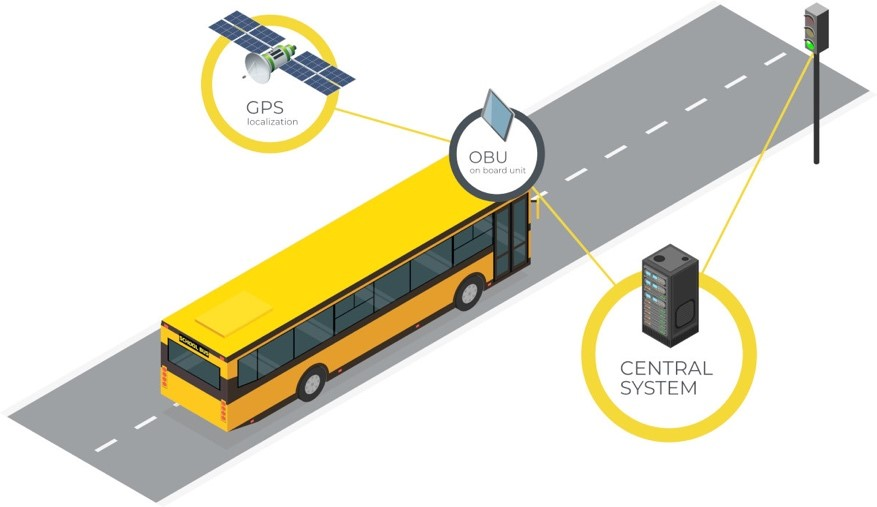
\includegraphics[width=0.7\linewidth]{image/pt_priority_system} \caption{Smart priority for public transport (SWARCO, 2021)}\label{fig:unnamed-chunk-10}
\end{figure}

\hypertarget{relevant-initiatives-in-austria-5}{%
\subsection*{Relevant initiatives in Austria}\label{relevant-initiatives-in-austria-5}}
\addcontentsline{toc}{subsection}{Relevant initiatives in Austria}

\begin{itemize}
\tightlist
\item
  \href{https://digitales.wien.gv.at/site/open-data/}{digitales.wien.gv.at}
\item
  \href{https://www.wienerlinien.at/eportal3/ep/channelView.do/pageTypeId/66528/channelId/-4400661}{wienerlinien.at}
\item
  \href{https://www.kapsch.net/ktc/Portfolio/IMS/Congestion/Managed-lanes}{kapsch.net-1}
\item
  \href{https://www.kapsch.net/ktc/Portfolio/IMS/Smart-Urban-Mobility/Urban-Mobility-Management}{kapsch.net-2}
\item
  \href{https://www.swarco.com/de/loesungen/oeffentlicher-nahverkehr/vorrang-fuer-den-oeffentlichen-nahverkehr}{swarco.com}
\item
  \href{https://www.mobility.siemens.com/global/de/portfolio/strasse/verkehrsmanagement/auf-der-strasse/smart-detection.html}{mobility.siemens.com}
\end{itemize}

\hypertarget{impacts-with-respect-to-sustainable-development-goals-sdgs-5}{%
\subsection*{Impacts with respect to Sustainable Development Goals (SDGs)}\label{impacts-with-respect-to-sustainable-development-goals-sdgs-5}}
\addcontentsline{toc}{subsection}{Impacts with respect to Sustainable Development Goals (SDGs)}

\begin{longtable}[]{@{}
  >{\centering\arraybackslash}p{(\columnwidth - 8\tabcolsep) * \real{0.2029}}
  >{\centering\arraybackslash}p{(\columnwidth - 8\tabcolsep) * \real{0.1884}}
  >{\centering\arraybackslash}p{(\columnwidth - 8\tabcolsep) * \real{0.2029}}
  >{\centering\arraybackslash}p{(\columnwidth - 8\tabcolsep) * \real{0.2029}}
  >{\centering\arraybackslash}p{(\columnwidth - 8\tabcolsep) * \real{0.2029}}@{}}
\toprule()
\begin{minipage}[b]{\linewidth}\centering
Impact level
\end{minipage} & \begin{minipage}[b]{\linewidth}\centering
Indicator
\end{minipage} & \begin{minipage}[b]{\linewidth}\centering
Impact direction
\end{minipage} & \begin{minipage}[b]{\linewidth}\centering
Goal description and number
\end{minipage} & \begin{minipage}[b]{\linewidth}\centering
Source
\end{minipage} \\
\midrule()
\endhead
Individual & Higher equality for people who do not drive & \textbf{+} & Equality (\emph{5,10}) & Litman, 2017; Cervero, 2013 \\
Individual & Less travel time for public transport users, more travel time for car users & \textbf{\textasciitilde{}} & Sustainable economic development (\emph{8,11}) & Seredynski et al., 2015 \\
Systemic & Public transport becomes more competitive compared to other transport modes & \textbf{+} & Equality (\emph{5,10}) & Schwendinger, 2019 \\
Systemic & Less fuel consumption & \textbf{+} & Environmental sustainability (\emph{7,12,13,15}) & Gassel et al., 2012; Seredynski et al., 2015 \\
Systemic & Transit is often the most cost-effective mode & \textbf{+} & Sustainable economic development (\emph{8,11}) & Litman, 2015 \\
Systemic & More infrastructure for public transport & \textbf{+} & Innovation \& Infrastructure (\emph{9}) & Cuthill et al., 2019 \\
\bottomrule()
\end{longtable}

\hypertarget{technology-and-societal-readiness-level-5}{%
\subsection*{Technology and societal readiness level}\label{technology-and-societal-readiness-level-5}}
\addcontentsline{toc}{subsection}{Technology and societal readiness level}

\begin{longtable}[]{@{}cc@{}}
\toprule()
TRL & SRL \\
\midrule()
\endhead
4-8 & 5-8 \\
\bottomrule()
\end{longtable}

\hypertarget{open-questions-5}{%
\subsection*{Open questions}\label{open-questions-5}}
\addcontentsline{toc}{subsection}{Open questions}

\begin{enumerate}
\def\labelenumi{\arabic{enumi}.}
\tightlist
\item
  Who is responsible for the implementation of PTP systems?
\item
  How will Vehicle-to-Vehicle (V2V), Vehicle-to-Infrastructure (V2I) and in future Vehicle-to-Pedestrian (V2P) change PTP systems?
\item
  How could also emergency vehicles be prioritised?
\item
  How to deal with mixed fleets - half new, half old?
\item
  What are the benefits compared to the costs?
\item
  Which standards should be used?
\end{enumerate}

\hypertarget{references-5}{%
\subsection*{References}\label{references-5}}
\addcontentsline{toc}{subsection}{References}

\begin{itemize}
\tightlist
\item
  Cervero, R. (2013). Bus rapid transit (BRT): An efficient and competitive mode of public transport (No.~2013-01). Working Paper.
\item
  Cuthill, N., Cao, M., Liu, Y., Gao, X., \& Zhang, Y. (2019). The association between urban public transport infrastructure and social equity and spatial accessibility within the urban environment: An investigation of Tramlink in London. Sustainability, 11(5), 1229.
\item
  Figenbaum, E., Fearnley, N., Pfaffenbichler, P., Hjorthol, R., Kolbenstvedt, M., Jellinek, R., \ldots{} \& Iversen, L. M. (2015). Increasing the competitiveness of e-vehicles in Europe. European transport research review, 7(3), 1-14.
\item
  Gassel, C., Matschek, T., \& Krimmling, J. (2012). Cooperative traffic signals for energy efficient driving in tramway systems. Aspekte der Verkehrstelematik--ausgewählte Veröffentlichungen 2012, 1.
\item
  Haitao, H., Yang, K., Liang, H., Menendez, M., \& Guler, S. I. (2019). Providing public transport priority in the perimeter of urban networks: A bimodal strategy. Transportation Research Part C: Emerging Technologies, 107, 171-192.
\item
  Litman, T. (2015). Evaluating public transit benefits and costs. Victoria, BC, Canada: Victoria Transport Policy Institute.
\item
  Litman, T. (2017). Evaluating Transportation Diversity. Victoria Transport Policy Institute.
\item
  Schwendinger, M. (2019). Vorrang für Busse und Straßenbahnen in Städten. \url{https://vcoe.at/files/vcoe/uploads/Projekte/Factsheets} 2019 Neu/VCÖ-Factsheet ÖV-Bevorrangen.pdf
\item
  Seredynski, M., Khadraoui, D., \& Viti, F. (2015, October). Signal phase and timing (SPaT) for cooperative public transport priority measures. In Proc. 22nd ITS World Congress.
\item
  Seredynski, M., Ruiz, P., Szczypiorski, K., \& Khadraoui, D. (2014, May). Improving bus ride comfort using GLOSA-based dynamic speed optimisation. In 2014 IEEE International Parallel \& Distributed Processing Symposium Workshops (pp.~457-463). IEEE.
\item
  Seredynski, M., \& Viti, F. (2017, October). Novel C-ITS support for electric buses with opportunity charging. In 2017 IEEE 20th International Conference on Intelligent Transportation Systems (ITSC) (pp.~1-6). IEEE.
\item
  Stahlmann, R., Möller, M., Brauer, A., German, R., \& Eckhoff, D. (2018). Exploring GLOSA systems in the field: Technical evaluation and results. Computer Communications, 120, 112-124.
\item
  SWARCO. (2021). Vorrang für den ÖPNV: Öffentliche Verkehrsmittel attraktiver machen. Available at: \url{https://www.swarco.com/de/loesungen/oeffentlicher-nahverkehr/vorrang-fuer-den-oeffentlichen-nahverkehr} {[}Accessed: 26 January 2021{]}
\item
  WIENER STADTWERKE GmbH. (2018). Wiener Linien: Autos auf Busspuren halten Öffis auf. Available at: \url{https://www.wienerstadtwerke.at/eportal3/ep/contentView.do?pageTypeId=71954\&channelId=-51313\&programId=72863\&contentId=4202309\&contentTypeId=1001} {[}Accessed: 30 September 2021{]}
\end{itemize}

\hypertarget{transformation_public_space}{%
\section{Transformation of public space and digital solutions}\label{transformation_public_space}}

\hypertarget{definition-6}{%
\subsection*{Definition}\label{definition-6}}
\addcontentsline{toc}{subsection}{Definition}

The digitalisation of public (and urban) spaces has been developing, giving rise to concepts such as smart city, wise city, U-city, intelligent city etc. However, its real acceleration started in 2010s as a result of industrial initiatives focused on the collection, management, processing and near real-time analysis of big data through the wide-spread of sensors connecting urban spaces, known as Internet of Things (IoT) devices. In the recent years, especially since the outbreak of COVID-19 pandemic, the urban digitalisation reached a new level. For example, in China digital systems for mass surveillance based on facial recognition are being deployed and in other parts of the world legal basis (such as General Data Protection Regulation (GDPR)) have been developed to allow for recording of biometric data in public spaces (Languillon-Aussel, 2021). Beyond surveillance, digitalisation of public spaces is used in many different areas such as payments and pricing, participatory tools or law enforcement, where, for example, in 2020 Singapore initiated the satellite-based urban toll system which allows for tracking any vehicle at any time of the day to implement dynamic pricing for road use and zone access (Languillon-Aussel, 2021).

Current approaches to the digitalisation of public spaces include mobiles apps, high resolution cameras, interactive stands and kiosks providing services and information, but also IoT devices such as sensors and beacons that automatically collect the data. These devices bring potential to improve the quality and coverage of service in public spaces, lower provision and delivery costs, increase safety and security. Nonetheless, they are not without challenges. Potential issues arise due to privacy and security concerns especially when private sector plays a key role (Warbis, 2018), potential technical difficulties such as unreliable Internet connection or unstable electricity supply (Haldrup, 2018) as well as low trust among society members and so-called \emph{digital exclusion} of certain social groups (Durand \& Zijlstra, 2020).

\hypertarget{key-stakeholders-6}{%
\subsection*{Key stakeholders}\label{key-stakeholders-6}}
\addcontentsline{toc}{subsection}{Key stakeholders}

\begin{itemize}
\tightlist
\item
  \textbf{Affected}: Citizens
\item
  \textbf{Responsible}: Local and national governments, Private technology companies, Citizens
\end{itemize}

\hypertarget{current-state-of-art-in-research-6}{%
\subsection*{Current state of art in research}\label{current-state-of-art-in-research-6}}
\addcontentsline{toc}{subsection}{Current state of art in research}

The research shows that as a result of higher digitalisation of public spaces and, in particular, increased digitalisation of transport, some groups may become \emph{digitally excluded}. The factors that are linked to vulnerability in terms of access to digitally-based services and transport are:

\begin{itemize}
\tightlist
\item
  \textbf{Age}: The elderly and underaged are particularly disadvantaged due to their lower engagement with technology. In the case of elderly population, the reduction in cognitive abilities and a decline in psychological mechanisms mean that in general, coping with new technologies can be difficult (Harvey et al., 2019; Pangbourne et al., 2010; Durand \& Zijlstra, 2020). On the other hand, children frequently do not have access to digitals forms of payment or cannot use all available modes of transport alone (Durand \& Zijlstra, 2020).
\item
  \textbf{Income and educational level}: People with lower income and education levels are more vulnerable to digital exclusion where, for example, a Dutch report shows that the transition from the offline to the online purchase of a yearly public transport subscription causes issues for people with lower income levels (Durand \& Zijlstra, 2020).
\item
  \textbf{Ethnicity}: The individuals from minorities tend to be more disadvantaged, however, this is frequently linked to other contributing factors such as cultural preferences or economic deprivation (Durand \& Zijlstra, 2020).
\end{itemize}

\hypertarget{current-state-of-art-in-practice-6}{%
\subsection*{Current state of art in practice}\label{current-state-of-art-in-practice-6}}
\addcontentsline{toc}{subsection}{Current state of art in practice}

At the beginning the digitalization of cities and public spaces strongly relied on the hidden, underground network of cables, sensors, connectors and masts which did not play significant role in the everyday life of an average citizen. Nowadays, the digitalization of public spaces incorporates the concept of smart city into the day-to-day life to a much larger extent. There are many ways in which digitalization materializes in public spaces.

One of them is improved \textbf{connectivity} in the form of Wi-Fi hotspots and zones. For example, in New York \href{https://www.link.nyc/}{LinkNYC} created connectivity corridors across five districts where more than 1700 links has allowed approximately 5 million users to connect for free to the country's fastest, most robust public fibre network. Through this service, \emph{LinkNYC} has supported people in accessing charities, using council services, and even applying for jobs (Warbis, 2018). Moreover, \href{https://calvium.com/}{Calvium} uses the improved connectivity to build a sense-of-place through digital-physical journeys of history and heritage, such as in \href{https://calvium.com/projects/battersea-power-station-redevelopment/}{Battersea Power Station} in London (Warbis, 2018).

Then, digitalisation brings the \textbf{transformation of public services} where non-personal data collected from public spaces is used to better understand the users of public spaces and their needs to improve the cities' spaces, infrastructure and provision of public services. For instance, looking at the type of devices connected to WiFi spots or engaging in digital place-making scheme might indicate socio-economic profiles and support councils in delivering the right services to the right people.

Two of such examples are (\emph{1}) \href{https://lbbd.emu-analytics.net/main/(view/950db2c7-1a3b-448d-9b21-444a0ec7b5e0//rightBar:appinfo)?basemapDetail=1\&zoom=5.0\&lng=-0.36613\&lat=54.04187}{Borough Data Explorer} that gathers data for the indicators that either contribute to borough's so-called \emph{Borough Manifesto targets} or feature within borough's \emph{social progress index} (Lbbd.emu-analytics.net, 2021). (\emph{2}) The Australian city of Joondalup partnered with \href{https://www.lakesidejoondalup.com.au/store-directory/telstra-shop/}{Telstra} to test IoT technologies to better monitor environmental factors like temperature, humidity, pollution, light and noise levels in real time (Barns, 2017).

Next, a \textbf{public-private partnership} is crucial for the strong and reliable digital public domain, where technology companies need to understand policy and strategy of local government to identify areas that may be supported through digital deployment. On the other hand, it is important for local government to understand the features of the technology for deployment. This tight cooperation enables the public sector to direct the digitisation of places in ways that work for public good, retaining the publicness of space and place, regardless of who owns, oversees or manages technologies being deployed (Warbis, 2018). The examples of such initiatives are \href{https://wegfinder.at/presse/2021/mit-wegfinder-ist-mobility-as-a-service-in-oesterreich-angekommen(1)/}{ÖBB360 wegfinder}, \href{https://austriatech.at/en/insight-into-the-work-of-the-urban-mobility-laboratories/}{Living Labs} and \href{https://www.aspern-seestadt.at/en}{Seestadt Wien}.

Within transport network the digitalisation brings benefits of improved customisation, efficiency and comfort. The examples of such efforts are real-time information on parking spaces availability such as \href{https://www.eparkomat.com/}{eParkomat} in Czech Republic, digital ticketing and scheduling, for instance, \href{https://www.dv-ticketing.com/}{DV Ticketing} or \href{https://www.thetrainline.com/}{Trainline} in the UK, electronic system for car and bike sharing fleets such as \href{https://www.share-now.com/at/en/}{Share-now} or \href{https://www.nextbike.at/de/niederoesterreich/}{Nextbike} etc. For more information on bike and car sharing see sections on \protect\hyperlink{bike_sharing}{bicycle and e-bicycle hire} and \protect\hyperlink{car_sharing}{car sharing} in this work.

Finally, public spaces are claimed to be political in nature. In Europe they support and condition the expression of the life in the city and play a role in participatory planning (Languillon-Aussel, 2021; Parkinson, 2012). For example, in 2013 Austrian railways ÖBB aimed at building a \href{https://www.partizipation.at/gueterzentrum_sued.html}{new freight centre} in Vienna that would move freight traffic away from the roads and onto the railways. The new freight centre was meant to replace the one at north-west station (Nordwestbahnhof). From the beginning, the project was intended to actively involve the general public, and the stakeholders were also strongly integrated into the planning. Therefore, before the start of the project, the ÖBB held an information event, which was accompanied by great protests (from the public) against the project. ÖBB tried, probably for this very reason, to involve the stakeholders so intensively in the entire planning process and as a result successfully completed the project.

Therefore, the digitalisation of urban spaces can influence the innovation in participatory tools where it allows the citizens to express opinion and provide feedback to actively contribute to infrastructure planning process and decision-making. This trend gave rise to so-called digital participatory planning (DPP) (Bouzguenda et al., 2020). Some examples of such initiatives include \href{https://mapyour.city/}{Map your city} app, ideas generation platform \href{https://www.involve.org.uk/resources/case-studies/decide-madrid}{Decide Madrid}, \href{https://oscity.nl/}{Open Source City} in the Netherlands, UK feedback platforms \href{https://www.involve.org.uk/resources/knowledge-base/what/public-participation}{Involve} and \href{http://www.changify.org/}{Changify} or arguments visualisation platform called \href{https://www.nesta.org.uk/feature/six-pioneers-digital-democracy/vtaiwan/}{vTaiwan}.

\hypertarget{relevant-initiatives-in-austria-6}{%
\subsection*{Relevant initiatives in Austria}\label{relevant-initiatives-in-austria-6}}
\addcontentsline{toc}{subsection}{Relevant initiatives in Austria}

\begin{itemize}
\tightlist
\item
  \href{https://wegfinder.at/presse/2021/mit-wegfinder-ist-mobility-as-a-service-in-oesterreich-angekommen(1)/}{ÖBB360 wegfinder}
\item
  \href{https://austriatech.at/en/insight-into-the-work-of-the-urban-mobility-laboratories/}{Living Labs}
\item
  \href{https://www.aspern-seestadt.at/en}{Seestadt Wien}
\item
  \href{https://ec.europa.eu/regional_policy/en/projects/Austria/support-for-digital-transformation-in-lower-austria}{House of digitalisation}
\end{itemize}

\hypertarget{impacts-with-respect-to-sustainable-development-goals-sdgs-6}{%
\subsection*{Impacts with respect to Sustainable Development Goals (SDGs)}\label{impacts-with-respect-to-sustainable-development-goals-sdgs-6}}
\addcontentsline{toc}{subsection}{Impacts with respect to Sustainable Development Goals (SDGs)}

\begin{longtable}[]{@{}
  >{\centering\arraybackslash}p{(\columnwidth - 8\tabcolsep) * \real{0.2029}}
  >{\centering\arraybackslash}p{(\columnwidth - 8\tabcolsep) * \real{0.1884}}
  >{\centering\arraybackslash}p{(\columnwidth - 8\tabcolsep) * \real{0.2029}}
  >{\centering\arraybackslash}p{(\columnwidth - 8\tabcolsep) * \real{0.2029}}
  >{\centering\arraybackslash}p{(\columnwidth - 8\tabcolsep) * \real{0.2029}}@{}}
\toprule()
\begin{minipage}[b]{\linewidth}\centering
Impact level
\end{minipage} & \begin{minipage}[b]{\linewidth}\centering
Indicator
\end{minipage} & \begin{minipage}[b]{\linewidth}\centering
Impact direction
\end{minipage} & \begin{minipage}[b]{\linewidth}\centering
Goal description and number
\end{minipage} & \begin{minipage}[b]{\linewidth}\centering
Source
\end{minipage} \\
\midrule()
\endhead
Individual & Diminished access to digitally based transport services for certain groups & \textbf{-} & Equality (\emph{5,10}) & Durand \& Zijlstra, 2020 \\
Systemic & Reduced risk for transport-related social exclusion & \textbf{+} & Equality (\emph{5,10}) & Harvey et al., 2019; Pangbourne et al., 2010 \\
Systemic & More informed planning and decision-making based on real-time data from IoT & \textbf{+} & Innovation \& Infrastructure (\emph{9}) & Barns, 2017, Bouzguenda et al., 2020 \\
Systemic & Increased collaboration between public and private sector & \textbf{+} & Partnership \& collaborations (\emph{17}) & Warbis, 2018; \\
\bottomrule()
\end{longtable}

\hypertarget{technology-and-societal-readiness-level-6}{%
\subsection*{Technology and societal readiness level}\label{technology-and-societal-readiness-level-6}}
\addcontentsline{toc}{subsection}{Technology and societal readiness level}

\begin{longtable}[]{@{}cc@{}}
\toprule()
TRL & SRL \\
\midrule()
\endhead
5-9 & 5-8 \\
\bottomrule()
\end{longtable}

\hypertarget{open-questions-6}{%
\subsection*{Open questions}\label{open-questions-6}}
\addcontentsline{toc}{subsection}{Open questions}

\begin{enumerate}
\def\labelenumi{\arabic{enumi}.}
\tightlist
\item
  To what extent does the increasingly important deployment of digital devices in public spaces impact their political dimensions?
\item
  Are digital technologies transforming citizen practices in public spaces and/or do they allow the emergence of new practices?
\item
  By allowing new forms of expression, as well as political and democratic participation online, the virtual space tends to become a new forum. Is digital technology capturing the political functions of public spaces, which have therefore become unnecessary?
\item
  What impacts do the short life cycles of technologies and the changes of technological generations have on the development of public spaces?
\item
  Is digital transforming the designs, shapes, dimensions, and spatiality of public spaces?
\item
  In what ways is the emergence of new tools and skills changing the way public spaces are planned and developed?
\item
  What role do digital technologies play in the representation, imagination, and perception of public spaces?
\item
  For which type(s) of recipient(s) (such as citizen, consumer, user, and inhabitant) are digital technologies deployed in the public space?
\item
  What impacts do they have on the populations frequenting public spaces?
\item
  Do digital technologies promote social exchanges, or on the contrary, do they physically replicate the segregation of digital bubbles?
\item
  What roles has digital played in adapting public spaces to the health crisis of COVID-19?
  (Languillon-Aussel, 2021)
\end{enumerate}

\hypertarget{further-links-4}{%
\subsection*{Further links}\label{further-links-4}}
\addcontentsline{toc}{subsection}{Further links}

\begin{itemize}
\tightlist
\item
  \href{https://agile-city.com/agile-city-research/digital-tools-for-participatory-led-design/}{Agile city}
\item
  \href{https://theconversation.com/surprise-digital-space-isnt-replacing-public-space-and-might-even-help-make-it-better-87173}{An article on city of bits}
\item
  \href{https://archer-soft.com/blog/how-build-real-time-parking-availability-system}{Parking management systems}
\item
  \href{https://jsis.washington.edu/news/internet-of-things-and-privacy-in-public/}{Internet of Things and Privacy in Public}
\end{itemize}

\hypertarget{references-6}{%
\subsection*{References}\label{references-6}}
\addcontentsline{toc}{subsection}{References}

\begin{itemize}
\tightlist
\item
  Barns, S. (2017) Surprise! Digital space isn't replacing public space, and might even help make it better. Available at: \url{https://theconversation.com/surprise-digital-space-isnt-replacing-public-space-and-might-even-help-make-it-better-87173} {[}Accessed: 12 April 2021{]}.
\item
  Bouzguenda, I., Alalouch, C., \& Fava, N. (2020). Examining digital participatory planning: maturity assessment in a small Dutch city. Journal of Cleaner Production, 264, 121706.
\item
  Durand, A. \& Zijlstra, T. (2020). The impact of digitalisation on the access to transport services: a literature review. 10.13140/RG.2.2.22686.97600.
\item
  Haldrup, S.,V. (2018). Digitising public service delivery: opportunities and limitations. Available at: \url{https://www.opml.co.uk/blog/digitising-public-service-delivery-opportunities-and-limitations} {[}Accessed: 12 April 2021{]}.
\item
  Harvey, J., Guo, W., \& Edwards, S. (2019). Increasing mobility for older travellers through engagement with technology. Transportation Research Part F: Traffic Psychology and Behaviour, 60, 172-184. \url{doi:10.1016/j.trf.2018.10.019}
\item
  Languillon-Aussel, R. (2021). Digitalisation of public spaces: the great urban change? Available at: \url{https://journals.openedition.org/articulo/4518} . {[}Accessed: 9 April 2021{]}
\item
  Lbbd.emu-analytics.net. (2021). Borough Data Explorer. Available at: \url{https://lbbd.emu-analytics.net/main/(view/950db2c7-1a3b-448d-9b21-444a0ec7b5e0//rightBar:appinfo)?basemapDetail=1\&zoom=4.7\&lng=3.34490\&lat=54.11363} {[}Accessed: 12 April 2021{]}.
\item
  Pangbourne, K. (2018). Mobility and Ageing: A Review of Interactions Between Transport and Technology from the Perspective of Older People In A. Curl \& C. Musselwhite (Eds.), Geographies of Transport and Ageing (pp.~51-71). Cham: Springer International Publishing.
\item
  Parkinson J., 2012, Democracy and Public Space: The Physical Sites of Democratic Performance, Oxford: Oxford University Press, 262 p.
\item
  Warbis, M. (2018). Making the Spaces of Cities Smarter: Why cities (and their citizens) should embrace the digital public realm. \textless Available at: \url{https://medium.com/@warbismichelle/making-the-spaces-of-cities-smarter-why-cities-should-embrace-the-digital-public-realm-c12afc810aaa}\textgreater. {[}Accessed: 12 April 2021{]}
\end{itemize}

\hypertarget{highway}{%
\chapter{Highway infrastructure management}\label{highway}}

\hypertarget{uav}{%
\section{Unmanned aerial vehicles for infrastructure maintenance}\label{uav}}

\hypertarget{synonyms-6}{%
\subsection*{Synonyms}\label{synonyms-6}}
\addcontentsline{toc}{subsection}{Synonyms}

\emph{Drones, remotely piloted vehicles, remotely piloted aircraft, uav}

\hypertarget{definition-7}{%
\subsection*{Definition}\label{definition-7}}
\addcontentsline{toc}{subsection}{Definition}

Unmanned Aerial Vehicles (UAVs), commonly known as drones are promising technologies that can be used in inspection and data gathering for infrastructure maintenance and management purposes. These include, for example, detection of wear and tear, monitoring of the progress at a highway construction site or the analysis of traffic (Frederiksen et al., 2019). UAVs typically include a portable control station for the human operator and under current legislation their operation in urban areas is limited to flying within visual line of sight (VLOS). UAVs typically feature various sensors and recorders, including video, far and near infra-red, radar or laser-based range finders and specialized communication devices (Shaghlil \& Khalafallah, 2018). Majority of them can transfer real-time data between the UAV and the control station. Moreover, some feature additional on-board data storage capabilities for enhanced data collection (Shaghlil \& Khalafallah, 2018). The use of drones for infrastructure-related tasks provide not only savings with respect to time, labour and costs, but they also allow for reduction in risks when dangerous operations usually performed by human can be substituted with drones. Finally, the environmental impact is diminished when drones, which produce considerably less CO\textsubscript{2}, are used instead of currently employed helicopters. Nevertheless, the use of drones as a tool for inspecting infrastructure can also pose certain challenges with respect to current technology, legal framework, privacy concerns and social acceptance.

\hypertarget{key-stakeholders-7}{%
\subsection*{Key stakeholders}\label{key-stakeholders-7}}
\addcontentsline{toc}{subsection}{Key stakeholders}

\begin{itemize}
\tightlist
\item
  \textbf{Affected}: Direct users of the roads and beneficiaries affected by the supply of transport services
\item
  \textbf{Responsible}: Government agencies responsible for planning, executing, and financing of maintenance activities, citizens, contractors and subcontractors, private companies and manufacturers
\end{itemize}

\hypertarget{current-state-of-art-in-research-7}{%
\subsection*{Current state of art in research}\label{current-state-of-art-in-research-7}}
\addcontentsline{toc}{subsection}{Current state of art in research}

Current research efforts and field trials-based studies are advocating the case of using UAVs for bridge inspection and monitoring. Previous study presented a proof of concept of utilising UAVs for bridge and high mast luminaires. Several experiments in controlled conditions were performed to test UAV response in relation to wind conditions. Moreover, image quality was examined in different flight scenarios, low light conditions, altitude and payload (Otero et al., 2015). Overall, the results are in favour of using drones for infrastructure inspections, not just in terms of saving human labour but also detecting the damages. The advantages of the drone use were also demonstrated in terms of reduced traffic control and decreased use of under bridge inspection vehicles (Zink and Lovelace, 2015). On the other hand, the lack of specific skills of the drone operators were found to hinder efficient use of drones for large-scale bridges (Wu et al., 2018). Further, some technological barriers also slow down the popularity of drones in infrastructure inspection, where an average flight time of the drone given its battery life is approximately 30 minutes. Therefore, current research aims at increasing the energy-efficiency by the use of path planning and algorithms to minimize energy utilization while maximizing coverage for traffic monitoring (Outay et al., 2020).

\hypertarget{current-state-of-art-in-practice-7}{%
\subsection*{Current state of art in practice}\label{current-state-of-art-in-practice-7}}
\addcontentsline{toc}{subsection}{Current state of art in practice}

Current use of drones is heavily regulated by national and international governments worldwide where the most considerable restriction is the requirement for drones to remain under VLOS of the controller. Beyond, the regulatory bodies put forward various specification with respect to physical aspects of the drones such as weight or sensors, training requirement of the operators and drones', data acquisition regulations and operation itself such as flight timeframe, altitude etc. (FAA, 2016; Outay at al., 2020). All of them, significantly restrict fast and wide application of drones in different areas. Therefore, the authorities attempt to provide regulations to tackle safety and privacy as well as noise concerns of the citizens. At the moment drones are used in oil and gas industry to conduct local surveys in off-shore facilities (Undertaking, 2016). Meanwhile in the transport sector, Danish company Dronops, after safety clearance, has been granted permission from Danish Road Authority to fly along a highway to monitor the traffic, where drone provides data from multiple sensors as well as video recordings. At the moment, the drone can only fly in good weather conditions and it is cable-linked to its power source located on the ground to allow for continuous day-long monitoring at 120 m above the ground. Importantly, the output data is used by Danish Road Authority and local council (Frederiksen et al., 2019).

\hypertarget{relevant-initiatives-in-austria-7}{%
\subsection*{Relevant initiatives in Austria}\label{relevant-initiatives-in-austria-7}}
\addcontentsline{toc}{subsection}{Relevant initiatives in Austria}

\begin{itemize}
\tightlist
\item
  \href{https://smartcity.wien.gv.at/site/en/smart-inspection/}{smartcity.wien}
\end{itemize}

\hypertarget{impacts-with-respect-to-sustainable-development-goals-sdgs-7}{%
\subsection*{Impacts with respect to Sustainable Development Goals (SDGs)}\label{impacts-with-respect-to-sustainable-development-goals-sdgs-7}}
\addcontentsline{toc}{subsection}{Impacts with respect to Sustainable Development Goals (SDGs)}

\begin{longtable}[]{@{}
  >{\centering\arraybackslash}p{(\columnwidth - 8\tabcolsep) * \real{0.2029}}
  >{\centering\arraybackslash}p{(\columnwidth - 8\tabcolsep) * \real{0.1884}}
  >{\centering\arraybackslash}p{(\columnwidth - 8\tabcolsep) * \real{0.2029}}
  >{\centering\arraybackslash}p{(\columnwidth - 8\tabcolsep) * \real{0.2029}}
  >{\centering\arraybackslash}p{(\columnwidth - 8\tabcolsep) * \real{0.2029}}@{}}
\toprule()
\begin{minipage}[b]{\linewidth}\centering
Impact level
\end{minipage} & \begin{minipage}[b]{\linewidth}\centering
Indicator
\end{minipage} & \begin{minipage}[b]{\linewidth}\centering
Impact direction
\end{minipage} & \begin{minipage}[b]{\linewidth}\centering
Goal description and number
\end{minipage} & \begin{minipage}[b]{\linewidth}\centering
Source
\end{minipage} \\
\midrule()
\endhead
Individual & Employees risk reduced & \textbf{+} & Health \& Wellbeing (\emph{3}) & Outay et al., 2020 \\
Systemic & Road safety increased & \textbf{+} & Health \& Wellbeing (\emph{3}) & Outay et al., 2020 \\
Systemic & Emissions rate reduced & \textbf{+} & Environmental sustainability (\emph{7,12,13,15}) & Outay et al., 2020 \\
Systemic & Job posts created & \textbf{+} & Sustainable economic development (\emph{8,11}) & Jenkins \& Vasigh, 2013 \\
Systemic & Faster road infrastructure innovation & \textbf{+} & Innovation \& Infrastructure (\emph{9}) & Fan \& Saadeghvaziri, 2019 \\
\bottomrule()
\end{longtable}

\hypertarget{technology-and-societal-readiness-level-7}{%
\subsection*{Technology and societal readiness level}\label{technology-and-societal-readiness-level-7}}
\addcontentsline{toc}{subsection}{Technology and societal readiness level}

\begin{longtable}[]{@{}cc@{}}
\toprule()
TRL & SRL \\
\midrule()
\endhead
3-4 & 5-7 \\
\bottomrule()
\end{longtable}

\hypertarget{open-questions-7}{%
\subsection*{Open questions}\label{open-questions-7}}
\addcontentsline{toc}{subsection}{Open questions}

\begin{enumerate}
\def\labelenumi{\arabic{enumi}.}
\tightlist
\item
  What are the factors influencing social acceptability of drones?
\item
  What actions from the policymakers need to be undertaken to minimalize cyber-attacks?
\item
  What aspects need to be considered by the governments before the integration of more sensors to record other relevant data along with the integration of video data with other geospatial information?
\end{enumerate}

\hypertarget{further-links-5}{%
\subsection*{Further links}\label{further-links-5}}
\addcontentsline{toc}{subsection}{Further links}

\begin{itemize}
\tightlist
\item
  \href{https://www.rolandberger.com/en/Insights/Publications/Drones-The-future-of-asset-inspection.html}{rolandberger}
\end{itemize}

\hypertarget{references-7}{%
\subsection*{References}\label{references-7}}
\addcontentsline{toc}{subsection}{References}

\begin{itemize}
\tightlist
\item
  FAA News, 2016, Summary of Small Unmanned Aircraft Rule (Part 107), Federal Aviation Authority, Washington DC, 20591, Accessed on May 2020, \url{https://www.faa.gov/uas/media/Part_107_Summary.pdf}.
\item
  Fan, J., \& Saadeghvaziri, M. A. (2019). Applications of Drones in Infrastructures: Challenges and Opportunities. International Journal of Mechanical and Mechatronics Engineering, 13(10), 649-655.
\item
  Frederiksen, M. H., Mouridsen, O. A. V., \& Knudsen, M. P. (2019). Drones for inspection of infrastructure: Barriers, opportunities and successful uses.
\item
  Jenkins, D., \& Vasigh, B. (2013). The economic impact of unmanned aircraft systems integration in the United States. Association for Unmanned Vehicle Systems International (AUVSI).
\item
  Otero, L.D., Gagliardo, N., Dalli, D., Huang, W.-H., Cosentino, P. (2015). Proof of concept for using unmanned aerial vehicles for high mast pole and bridge inspections (No.~BDV28-977-02). Florida. Dept. of Transportation. Research Center.
\item
  Outay, F., Mengash, H. A., \& Adnan, M. (2020). Applications of unmanned aerial vehicle (UAV) in road safety, traffic and highway infrastructure management: Recent advances and challenges. Transportation research. Part A, Policy and practice, 141, 116--129. \url{https://doi.org/10.1016/j.tra.2020.09.018}
\item
  Shaghlil, N., \& Khalafallah, A. (2018). Automating highway infrastructure maintenance using unmanned aerial vehicles. In Construction Research Congress (2-4).
\item
  Undertaking, S. J. (2016). European drones outlook study. Unlocking the Value for Europe.
\item
  Wu, W., Qurishee, M. A., Owino, J., Fomunung, I., Onyango, M., Atolagbe, B. (2018). Coupling deep learning and UAV for infrastructure condition assessment automation. In: 2018 IEEE International Smart Cities Conference (ISC2). IEEE, pp.~1--7.
\item
  Zink, J. and Lovelace, B., 2015. Unmanned aerial vehicle bridge inspection demonstration project. Research Project. Final Report, 40. Accessed in Nov 2020
\end{itemize}

\hypertarget{charging_station}{%
\section{Electric charging stations}\label{charging_station}}

\hypertarget{synonyms-7}{%
\subsection*{Synonyms}\label{synonyms-7}}
\addcontentsline{toc}{subsection}{Synonyms}

\emph{electric vehicle charging station, EV charging station, electric recharging point, charging point, electronic charging station (ECS), electric vehicle supply equipment (EVSE)}

\hypertarget{definition-8}{%
\subsection*{Definition}\label{definition-8}}
\addcontentsline{toc}{subsection}{Definition}

Nowadays, the use of electric vehicles is continuously increasing, hence it is not surprising that both, governments and private companies have strong interest in expanding EV charging infrastructure to ensure uninterrupted travelling and stimulate consumer adoption. There are three main types of charging stations, depending on the power output (measured in kilowatts (kW)) and consequently charging speed. These are:

\begin{itemize}
\tightlist
\item
  \textbf{Rapid}
\end{itemize}

They are the fastest way to charge an EV, therefore, this type is most frequently deployed near main routes and at highway service stations. They provide tethered cable and high power of direct (DC) or alternating current (AC). Vehicles can be charged in approximately 20 minutes up to 80\%, but, on average it takes about an hour for a new EV. \emph{Rapid DC} chargers use either \href{https://chademo.com/}{CHAdeMO} or CCS charging standards. These are two most popular types at the moment. They provide power of 50 kW. A newer type are \emph{Ultra Rapid DC} chargers that have power output of at least 100 kW. Further, \emph{Rapid AC} chargers provide power of 43 kW and use the \href{https://www.mobilityhouse.com/int_en/knowledge-center/charging-cable-and-plug-types\#:~:text=Type\%202\%20plug,-The\%20triple\%2Dphase\&text=In\%20private\%20spaces\%2C\%20charging\%20power,with\%20a\%20type\%202\%20socket.}{Type 2} charging standard. Finally, a special network of chargers are \emph{Tesla's superchargers} which are custom made for Tesla vehicles. Nonetheless, many Tesla drivers use adapters that enable them to use widely-available generic chargers (Lilly, 2020).

\begin{itemize}
\tightlist
\item
  \textbf{Fast}
\end{itemize}

Fast charging units typically provide AC charging with power output of 7kW or 22kW. Nevertheless, it is also possible to find stations that use 25 kW DC chargers with CHAdeMO or CCS charging standards. The charging times range between 1-6 hours depending on the battery installed in the vehicle. Fast chargers are usually located at the car parks, supermarkets, or leisure centres, where cars are likely be parked at for an hour or more. Fast charging units can be both tethered and untethered (Lilly, 2020).

\begin{itemize}
\tightlist
\item
  \textbf{Slow}
\end{itemize}

The power output of slow chargers varies between 2.3 kW to 6 kW and takes from 6 to 12 hours. Most slow charging units are untethered, meaning that the driver needs to supply his own cable to connect the EV with the charge point. They are usually used to charge at home overnight but also at workplace and at public points. Because of the longer charging times over fast units, slow public charge points are less common and may be older devices.

Finally, it is important to mention that the development of public EV charging stations is an important factor that influences the adoption of electric vehicles, nonetheless, the high investment costs (including land acquisition, installation, operation and maintenance) and low profitability (that heavily relies on their use) are considered key barriers to the faster development of charging stations (Lilly, 2020).

\hypertarget{key-stakeholders-8}{%
\subsection*{Key stakeholders}\label{key-stakeholders-8}}
\addcontentsline{toc}{subsection}{Key stakeholders}

\begin{itemize}
\tightlist
\item
  \textbf{Affected}: EV drivers
\item
  \textbf{Responsible}: National enterprises and governments, international oil and gas companies, automotive companies, start-ups in the green energy sector, transport authorities
\end{itemize}

\hypertarget{current-state-of-art-in-research-8}{%
\subsection*{Current state of art in research}\label{current-state-of-art-in-research-8}}
\addcontentsline{toc}{subsection}{Current state of art in research}

Charging stations for electric vehicles are now a well-established technology in itself. Therefore, current research focuses on the exploration of their potential when combined with other new technologies. For example, Lokhandwala \& Cai (2020) use New York City taxis as a case study to considers possible interactions between charging infrastructure for electric vehicles, ride sharing (RS) and autonomous vehicles (AV). For this purpose, they compare the optimal charging infrastructure expansion plans for three cases: non-AV-RS scenario (present), AV-RS scenario (future) and a mixed case. The study simulation shows that for the AV-RS case the use of charging stations is more spread throughout the day as compared to non-AV-RS where the demand and queuing are the highest in the mornings. In terms of the service levels, it is found that in the non-AV-RS scenario the service level remained unchanged as a result of the adoption of EV while in the AV-RS case, the level decreased by 2\%. Finally, the study shows that EV taxis were predicted to achieve reduction in CO\textsubscript{2} emission in both scenario types.

Additionally, a large strand of research focuses on optimising the locations of charging station for various vehicle types such as taxis (Zhang et al, 2019), buses (Uslu \& Kaya, 2021; Wu et al., 2021; He et al., 2019) and private EVs (Pan et al., 2020) considering different factors, for instance, social acceptance, EV adoption rate, demand fluctuations, trip length (Anjos et al., 2020) and road infrastructure types including highways (Napoli et al., 2020) and urban network (Ji et al., 2020).

Finally, an important part of the research looks at the role of charging station infrastructure in the adoption and use of electric vehicle which are considered a solution to reduce green-house gas emissions and air pollution (Philipsen et al., 2019; Bonges et al., 2016). For instance, the study by Melliger et al.~(2018) explored how the expansion of the charging station network can counteract phenomenon of so-called `\emph{range anxiety}' in EV buyers related to the capacity of EV battery and availability of charging point along the routes (Melliger et al., 2018).

\hypertarget{current-state-of-art-in-practice-8}{%
\subsection*{Current state of art in practice}\label{current-state-of-art-in-practice-8}}
\addcontentsline{toc}{subsection}{Current state of art in practice}

According to the Global EV outlook 2020 (IEA, 2020), the number of global charging stations reached 7.3 million chargers in 2019. Of this number, 6.5 million are slow and normal chargers which are installed at home, residential, and office buildings while the rest are publicly accessible chargers (Thananusak et al., 2021).

Denser network of charging stations has been showed to be an important factor in counteracting \emph{range anxiety} in EV users (Philipsen et al., 2019). Therefore, it is not surprising that policies of many countries in Europe and beyond set the goals for the construction of EV charging stations to encourage their uptake. For example, France introduced so-called \href{https://www.iea.org/policies/8737-law-on-energy-transition-for-green-growth-ltecv}{Law on Energy Transition for Green Growth (LTECV)} which aims at building 7 million charging station by 2030 (Thananusak et al., 2021). Similarly, in Switzerland the Federal Road Office (FEDRO) recommended installation of fast-charging stations at all main highway service areas (Melliger et al., 2018). In terms of EU-wide legislation, \emph{\href{https://eur-lex.europa.eu/legal-content/EN/TXT/HTML/?uri=CELEX:32014L0094\&from=en}{Directive 2014/94/EU} on the deployment of alternative fuels recharging and refuelling infrastructure} (known as Alternative Fuels Infrastructure Directive (AFI)) requires the EU member states to provide an appropriate number of publicly accessible charging points.
In Austrian context, the study by Baresch \& Moser (2019) showed that 88\% of EV users charges their cars at home and only 1.5\% - 1.7\% uses public stations. This significantly influences the profitability of public stations. To alleviate this problem, governments can use demand-push or technology-push policies. The demand-push solutions are based on extending the markets for innovations to induce the demand and increase the profits from charging station business. These include, for example, consumer awareness building, rebates and tax credits. On the other hand, the technology-push solutions are aimed at decreasing the cost of innovative solution, through funding and subsidies for R\&D in private sector (Thananusak et al., 2021).
Interestingly, between 2007 and 2013 first transnational electric mobility project took place between Vienna and Bratislava. It aimed at demonstrating the operationability of a cross-border initiative. For this purpose, a number of charging stations have been built in public and semi-public places to allow users of electric vehicles to charge their cars on either side of the border. The project showed the user-friendliness of electric vehicles in daily traffic and the trans-border availability of services, no matter what the country of residence of the e-mobility customer (Verbund, 2011).

\hypertarget{relevant-initiatives-in-austria-8}{%
\subsection*{Relevant initiatives in Austria}\label{relevant-initiatives-in-austria-8}}
\addcontentsline{toc}{subsection}{Relevant initiatives in Austria}

\begin{itemize}
\tightlist
\item
  \href{http://www.ieahev.org/by-country/austria-charging-infrastructure/}{ieahev.org}
\item
  \href{https://ev-charging.com/at/en/elektrotankstellen}{ev-charging.com}
\item
  \href{https://smatrics.com/en/charging-network}{smatrics.com}
\item
  \href{https://chargemap.com/cities/wien-AT}{chargemap.com}
\end{itemize}

\hypertarget{impacts-with-respect-to-sustainable-development-goals-sdgs-8}{%
\subsection*{Impacts with respect to Sustainable Development Goals (SDGs)}\label{impacts-with-respect-to-sustainable-development-goals-sdgs-8}}
\addcontentsline{toc}{subsection}{Impacts with respect to Sustainable Development Goals (SDGs)}

\begin{longtable}[]{@{}
  >{\centering\arraybackslash}p{(\columnwidth - 8\tabcolsep) * \real{0.2029}}
  >{\centering\arraybackslash}p{(\columnwidth - 8\tabcolsep) * \real{0.1884}}
  >{\centering\arraybackslash}p{(\columnwidth - 8\tabcolsep) * \real{0.2029}}
  >{\centering\arraybackslash}p{(\columnwidth - 8\tabcolsep) * \real{0.2029}}
  >{\centering\arraybackslash}p{(\columnwidth - 8\tabcolsep) * \real{0.2029}}@{}}
\toprule()
\begin{minipage}[b]{\linewidth}\centering
Impact level
\end{minipage} & \begin{minipage}[b]{\linewidth}\centering
Indicator
\end{minipage} & \begin{minipage}[b]{\linewidth}\centering
Impact direction
\end{minipage} & \begin{minipage}[b]{\linewidth}\centering
Goal description and number
\end{minipage} & \begin{minipage}[b]{\linewidth}\centering
Source
\end{minipage} \\
\midrule()
\endhead
Systemic & Contribution to emissions reduction (via EVs) & \textbf{+} & Environmental sustainability (\emph{7,12,13,15}) & Thananusak et al., 2021 \\
Systemic & Increased public funding on charging stations but high entry barriers for investors & \textbf{\textasciitilde{}} & Innovation \& Infrastructure (\emph{9}) & Thananusak et al., 2021 \\
Systemic & Encourages collaboration between different stakeholders (e.g.~Industry and Governments) and countries & \textbf{+} & Partnership \& collaborations (\emph{17}) & Thananusak et al., 2021 \\
\bottomrule()
\end{longtable}

\hypertarget{technology-and-societal-readiness-level-8}{%
\subsection*{Technology and societal readiness level}\label{technology-and-societal-readiness-level-8}}
\addcontentsline{toc}{subsection}{Technology and societal readiness level}

\begin{longtable}[]{@{}cc@{}}
\toprule()
TRL & SRL \\
\midrule()
\endhead
8-9 & 6-8 \\
\bottomrule()
\end{longtable}

\hypertarget{open-questions-8}{%
\subsection*{Open questions}\label{open-questions-8}}
\addcontentsline{toc}{subsection}{Open questions}

\begin{enumerate}
\def\labelenumi{\arabic{enumi}.}
\tightlist
\item
  What are demand-pull and technology-push policies to increase investment in EV charging stations? What is their relative effectiveness?
\item
  What share of car trips can be successfully covered with the currently available (2021) BEVs and the current charging infrastructure?
\item
  What are the needs of Austrian car users with respect to the driving range?
\end{enumerate}

\hypertarget{further-links-6}{%
\subsection*{Further links}\label{further-links-6}}
\addcontentsline{toc}{subsection}{Further links}

\begin{itemize}
\tightlist
\item
  \href{https://www.plugshare.com/en}{plugshare.com}
\item
  \href{https://www.dekra-product-safety.com/en/ev-charging-station-technology}{dekra-product-safety.com}
\end{itemize}

\hypertarget{references-8}{%
\subsection*{References}\label{references-8}}
\addcontentsline{toc}{subsection}{References}

\begin{itemize}
\tightlist
\item
  Anjos, M. F., Gendron, B., \& Joyce-Moniz, M. (2020). Increasing electric vehicle adoption through the optimal deployment of fast-charging stations for local and long-distance travel. European Journal of Operational Research, 285(1), 263-278.
\item
  Bonges III, H. A., \& Lusk, A. C. (2016). Addressing electric vehicle (EV) sales and range anxiety through parking layout, policy and regulation. Transportation Research Part A: Policy and Practice, 83, 63-73.
\item
  He, Y., Song, Z., \& Liu, Z. (2019). Fast-charging station deployment for battery electric bus systems considering electricity demand charges. Sustainable Cities and Society, 48, 101530.
\item
  IEA. (2020). Global EV Outlook 2020; IEA: Paris, France. p.~276.
\item
  Ji, D., Lv, M., Yang, J., \& Yi, W. (2020). Optimizing the Locations and Sizes of Solar Assisted Electric Vehicle Charging Stations in an Urban Area. IEEE Access, 8, 112772-112782.
\item
  Lilly, C., (2020). EV Charging connectors - Electric car charging speeds. Zap-Map. Available at: \url{https://www.zap-map.com/charge-points/connectors-speeds/\#:~:text=There\%20are\%20three\%20main\%20types,measured\%20in\%20kilowatts\%20(kW).} {[}Accessed: 26 March 2021{]}.
\item
  Lokhandwala, M., \& Cai, H. (2020). Siting charging stations for electric vehicle adoption in shared autonomous fleets. Transportation Research Part D: Transport and Environment, 80, 102231.
\item
  Melliger, M. A., van Vliet, O. P., \& Liimatainen, H. (2018). Anxiety vs reality--Sufficiency of battery electric vehicle range in Switzerland and Finland. Transportation Research Part D: Transport and Environment, 65, 101-115.
\item
  Napoli, G., Polimeni, A., Micari, S., Andaloro, L., \& Antonucci, V. (2020). Optimal allocation of electric vehicle charging stations in a highway network: Part 1. Methodology and test application. Journal of Energy Storage, 27, 101102.
\item
  Pan, L., Yao, E., Yang, Y., \& Zhang, R. (2020). A location model for electric vehicle (EV) public charging stations based on drivers' existing activities. Sustainable Cities and Society, 59, 102192.
\item
  Philipsen, R., Brell, T., Biermann, H., \& Ziefle, M. (2019). Under Pressure---Users' Perception of Range Stress in the Context of Charging and Traditional Refueling. World Electric Vehicle Journal, 10(3), 50.
\item
  Thananusak, T., Punnakitikashem, P., Tanthasith, S., \& Kongarchapatara, B. (2021). The Development of Electric Vehicle Charging Stations in Thailand: Policies, Players, and Key Issues (2015--2020). World Electric Vehicle Journal, 12(1), 2.
\item
  Uslu, T., \& Kaya, O. (2021). Location and capacity decisions for electric bus charging stations considering waiting times. Transportation Research Part D: Transport and Environment, 90, 102645.
\item
  Verbund.com (2011). Europe Premiere: Unlimited Electric Mobility - VERBUND. Verbund.com. Available at: \url{https://www.verbund.com/en-de/about-verbund/news-press/press-releases/2011/03/04/unlimited-electric-mobility} {[}Accessed: 26 March 2021{]}.
\item
  Wu, X., Feng, Q., Bai, C., Lai, C. S., Jia, Y., \& Lai, L. L. (2021). A novel fast-charging stations locational planning model for electric bus transit system. Energy, 120106.
\item
  Zhang, S., Wang, H., Zhang, Y. F., \& Li, Y. Z. (2019). A novel two-stage location model of charging station considering dynamic distribution of electric taxis. Sustainable Cities and Society, 51, 101752.
\end{itemize}

\hypertarget{traffic}{%
\chapter{Traffic management}\label{traffic}}

\hypertarget{congestion_charging}{%
\section{Congestion charging}\label{congestion_charging}}

\hypertarget{synonyms-8}{%
\subsection*{Synonyms}\label{synonyms-8}}
\addcontentsline{toc}{subsection}{Synonyms}

\emph{Congestion charging scheme, CCS}

\hypertarget{definition-9}{%
\subsection*{Definition}\label{definition-9}}
\addcontentsline{toc}{subsection}{Definition}

The congestion charging is an example of (urban) road pricing system aimed at reducing congestion and pollution in zones where it applies. The regulations and prices of congestion charges can vary based on spatial, temporal or modal basis (Santos, 2005). Congestion charges are used to influence the traffic demand and discourage the use of roads at congested times (Valletta, 2015). The major congestion charge zone in Europe was introduced in London in 2003 and it imposed a fee for all the vehicles that drove into or through the designated area in the city centre between 7:00 and 18:00 (Mon-Fri) (Munford, 2017). It included a 90\% discount for residents, nevertheless, at the time it was considered the most radical transport policy to have been implemented in the recent decades (Banister, 2003). Nearly 20 years later, congestion charges are an effective measure to protect city centres, used in several cities around the world such as London, Singapore, New York, Stockholm, Milan, Bergen or Gothenburg, even though they are still rather unpopular within the society. The research findings with respect of the effectiveness of this transport policy on a number of aspects are summarized in the \emph{research section}, below.

\hypertarget{key-stakeholders-9}{%
\subsection*{Key stakeholders}\label{key-stakeholders-9}}
\addcontentsline{toc}{subsection}{Key stakeholders}

\begin{itemize}
\tightlist
\item
  \textbf{Affected}: Local residents, car and truck drivers, motor bikers, cyclists, pedestrians
\item
  \textbf{Responsible}: Local and national governments, transport authorities
\end{itemize}

\hypertarget{current-state-of-art-in-research-9}{%
\subsection*{Current state of art in research}\label{current-state-of-art-in-research-9}}
\addcontentsline{toc}{subsection}{Current state of art in research}

Given that congestion charging has been used for some time now, the existing research focuses mainly on the effects of the introduction of congestion charges on different areas that may be affected, such as air quality, housing prices, traffic improvements, travel behaviour and road safety, economic aspects and social acceptability.

Starting with public attitude towards congestion charging schemes, it is fair to say that public opinion is divided and there are several factors which influence the outlook on this transport policy. For example, study by Grisolía et al.~(2015) showed the differences in acceptance levels between drivers and non-drivers, where the latter ones are more favourable to congestion charging systems. Moreover, Hamilton (2011) came to a similar conclusion where he found that higher frequency of car use was associated with lower acceptance of congestion charges. Further, the study showed that public acceptance of congestion charging is likely to increase with more experience with the charging system but also among individuals with high value of time and pro-environmental interests as well as those who are in favour of high degree of government intervention.

What is more, a number of studies showed that congestion charging has led to a significant improvement in traffic conditions where travel times decreased by 19\% on average. Beyond, 14.5\% decrease of the private vehicles' presence in the affected area was observed and the use of public transport increased by up to 18\% (What Works Centre for Local Economic Growth, 2020; Gibson \& Carnovale, 2015; Amelsfort \& Swedish, 2015).

With respect to road safety the results are ambiguous depending on the location. For example, the road safety improved in London and Milan, however in Rome it deteriorated following the switch from cars to motorcycles leading to higher accidents rate (Amelsfort \& Swedish, 2015).

Next, a number of studies demonstrated the positive impact of congestion charges on air pollution within the targeted zones, where the levels of CO\textsubscript{2} decreased by 19.5\% on average and NO\textsubscript{x} (nitrogen oxides) decreased by 10.5\% (Amelsfort \& Swedish, 2015).

In terms of economic effects, it has been showed that implementation of congestion charges can increase house values within the zone (potentially due to additional exemptions for residents). For example, following the introduction of congestion charge in London residential property values rose by 5\%. At the same time, congestion charging can lead to a reduction in retail property values. In Singapore after the implementation of road pricing scheme the retail real estate prices decreased in the targeted zone (Amelsfort \& Swedish, 2015; Agarwal, 2015). Further, study by Percoco (2014) found that the introduction of road pricing system reduced house prices in the affected zone. In conclusion, literature shows a mixed effect of congestion charges on property values, depending on specific location and additional regulation and exceptions that are in place.

\hypertarget{current-state-of-art-in-practice-9}{%
\subsection*{Current state of art in practice}\label{current-state-of-art-in-practice-9}}
\addcontentsline{toc}{subsection}{Current state of art in practice}

Nowadays there are different functioning models of congestion charging schemes around the world. One broadly used model is the \emph{zone/cordon-based charges} which is based on the idea of geographic boundary so that charges are implemented when entering or leaving the zone (or both). Henceforth, travellers within the zone do not incur the cost. This contrasts with so-called \emph{area charging} where the fees apply to all the drivers travelling or parking within the designated area. The first one may be thought of as a `per passage charge' and the latter `once per 24h charge' when the fees are charged daily. Cordon-based charging is currently used in multiple Norwegian cities (e.g.~Bergen and Oslo), Milan or Durham while area charging systems is present in London.

What is more, initially a number of exemptions were available for low emission and alternative fuel vehicles such as all-electric cars and plug-in hybrids however local authorities gradually moved away from these discounts (Chris, 2016). For example, in Vienna there are several regulations for the entry of company vehicles with different levels of emissions into the city centre. These were first introduced in 2014 and they require all the business vehicles to have an environmental badge known as `Umwelt Pickerl' to access the city. Moreover, there is an `Emergency Scheme' in Vienna which becomes effective as soon as the certain pollution limits are exceeded. As a result, and depending on the severity of the event, either a recommendation to switch to public transport is announced or vehicles with internal combustion engines can be banned from driving (Sadler Consultants Ltd, 2021).

\hypertarget{relevant-initiatives-in-austria-9}{%
\subsection*{Relevant initiatives in Austria}\label{relevant-initiatives-in-austria-9}}
\addcontentsline{toc}{subsection}{Relevant initiatives in Austria}

\begin{itemize}
\tightlist
\item
  \href{https://urbanaccessregulations.eu/countries-mainmenu-147/austria-mainmenu-78/wien-vienna}{urbanaccessregulations.eu}
\item
  \href{https://www.environmentalbadge.com/environmental-zone-vienna/}{environmentalbadge.com}
\end{itemize}

\hypertarget{impacts-with-respect-to-sustainable-development-goals-sdgs-9}{%
\subsection*{Impacts with respect to Sustainable Development Goals (SDGs)}\label{impacts-with-respect-to-sustainable-development-goals-sdgs-9}}
\addcontentsline{toc}{subsection}{Impacts with respect to Sustainable Development Goals (SDGs)}

\begin{longtable}[]{@{}
  >{\centering\arraybackslash}p{(\columnwidth - 8\tabcolsep) * \real{0.2029}}
  >{\centering\arraybackslash}p{(\columnwidth - 8\tabcolsep) * \real{0.1884}}
  >{\centering\arraybackslash}p{(\columnwidth - 8\tabcolsep) * \real{0.2029}}
  >{\centering\arraybackslash}p{(\columnwidth - 8\tabcolsep) * \real{0.2029}}
  >{\centering\arraybackslash}p{(\columnwidth - 8\tabcolsep) * \real{0.2029}}@{}}
\toprule()
\begin{minipage}[b]{\linewidth}\centering
Impact level
\end{minipage} & \begin{minipage}[b]{\linewidth}\centering
Indicator
\end{minipage} & \begin{minipage}[b]{\linewidth}\centering
Impact direction
\end{minipage} & \begin{minipage}[b]{\linewidth}\centering
Goal description and number
\end{minipage} & \begin{minipage}[b]{\linewidth}\centering
Source
\end{minipage} \\
\midrule()
\endhead
Individual & Social contacts within zone reduced \& air quality improved & \textbf{\textasciitilde{}} & Health \& Wellbeing (\emph{3}) & Munford, 2017; Beevers \& Carslaw, 2005 \\
Individual & Increased costs of car use & \textbf{-} & Equality (\emph{5,10}) & Amelsfort \& Swedish, 2015 \\
Individual & Ambiguous effect on housing value & \textbf{\textasciitilde{}} & Sustainable economic development (\emph{8,11}) & Keat Tang, 2016 \\
Systemic & Reduced emissions \& increased use of public transport within the affected zone & \textbf{+} & Environmental sustainability (\emph{7,12-13,15}) & Beevers \& Carslaw, 2005; Gibson \& Carnovale, 2015 \\
Systemic & Increased revenues from charges \& increased use of public transport & \textbf{+} & Sustainable economic development (\emph{8,11}) & Amelsfort \& Swedish, 2015 \\
\bottomrule()
\end{longtable}

\hypertarget{technology-and-societal-readiness-level-9}{%
\subsection*{Technology and societal readiness level}\label{technology-and-societal-readiness-level-9}}
\addcontentsline{toc}{subsection}{Technology and societal readiness level}

\begin{longtable}[]{@{}cc@{}}
\toprule()
TRL & SRL \\
\midrule()
\endhead
7-9 & 5-7 \\
\bottomrule()
\end{longtable}

\hypertarget{open-questions-9}{%
\subsection*{Open questions}\label{open-questions-9}}
\addcontentsline{toc}{subsection}{Open questions}

\begin{enumerate}
\def\labelenumi{\arabic{enumi}.}
\tightlist
\item
  What are the implications of congestion charges on overall welfare in the affected zone?
\item
  What are the effects of different congestion charge designs such as exemptions of different nature?
\item
  What effect the implementation of congestion charge zone will have on the traffic in neighbouring areas (due to e.g.~re-routing)?
\item
  What is the potential for expansion of more sustainable transport mode within the targeted zone?

  \begin{itemize}
  \tightlist
  \item
    What is the actual modal split?
  \item
    What is the proportion of road space occupied by different modes?
  \item
    What is the potential of future investment in public transport?
  \item
    To what extent road capacity is used for parking (formally and informally)? (Van Amelsfort \& Swedish, 2015)
  \end{itemize}
\end{enumerate}

\hypertarget{further-links-7}{%
\subsection*{Further links}\label{further-links-7}}
\addcontentsline{toc}{subsection}{Further links}

\begin{itemize}
\tightlist
\item
  \href{https://whatworksgrowth.org/policy-reviews/transport/congestion-charging}{whatworksgrowth.org}
\item
  \href{https://www.adb.org/sites/default/files/publication/159940/introduction-congestion-charging.pdf}{adb.org}
\item
  \href{http://www.epomm.eu/newsletter/v2/content/2015/0415/doc/eupdate_en.pdf}{epomm.eu}
\end{itemize}

\hypertarget{references-9}{%
\subsection*{References}\label{references-9}}
\addcontentsline{toc}{subsection}{References}

\begin{itemize}
\tightlist
\item
  Agarwal, Sumit, Koo, Kang Mo, \& Sing, Tien Foo. (2015). ``Impact of electronic road pricing on real estate prices in Singapore.'' Journal of Urban Economics, 90, 50--59.
\item
  Banister, D. (2003). Critical pragmatism and congestion charging in London. International Social Science Journal, 55(176), 249-264.
\item
  Beevers, S. D., \& Carslaw, D. C. (2005). The impact of congestion charging on vehicle emissions in London. Atmospheric Environment, 39(1), 1-5.
  Lilly, Chris (2016). Congestion charge sunset period ends today. Next Green Car. Available at:
  \url{https://www.nextgreencar.com/news/7701/congestion-charge-sunset-period-ends-today/} {[}Accessed: 3 February 2021{]}
\item
  Gibson, M., and Carnovale, M. (2015). ``The effects of road pricing on driver behaviour and air pollution'' Journal of Urban Economics, 89, pp.~62-73.
\item
  Grisolía, J. M., López, F., \& de Dios Ortúzar, J. (2015). Increasing the acceptability of a congestion charging scheme. Transport Policy, 39, 37-47.
\item
  Hamilton, C. J. (2011). Popular Acceptance of Congestion Charging.
\item
  Keat Tang, C. (2016). ``The Cost of Traffic: Evidence from the London Congestion Charge'' SERC discussion paper 205
\item
  Munford, L. A. (2017). The impact of congestion charging on social capital. Transportation Research Part A: Policy and Practice, 97, 192-208.
\item
  Percoco, M. (2014). ``The impact of road pricing on housing prices: Preliminary evidence from Milan'' Transportation Research Part A Policy and Practice, 67, pp.~188-194.
\item
  Sadler Consultants Ltd (2021). Wien (Vienna). Urbanaccessregulations.eu. Available at: \url{https://urbanaccessregulations.eu/countries-mainmenu-147/austria-mainmenu-78/wien-vienna} {[}Accessed: 3 February 2021{]}.
\item
  Santos, G. (2005). Urban congestion charging: a comparison between London and Singapore. Transport Reviews, 25(5), 511-534.
\item
  What Works Centre for Local Economic Growth (2020). Evidence Review: Congestion charging. Available at: \url{https://whatworksgrowth.org/public/files/Evidence_reviewed_examples/Congestion_charging_-_Evidence_review.pdf} {[}Accessed: 2 February 2021{]}.
\item
  Van Amelsfort, D., \& Swedish, V. (2015). Introduction to congestion charging: A guide for practitioners in developing cities.
\item
  Valletta, M. (2015) Congestion charging in Europe.
\end{itemize}

\hypertarget{platooning}{%
\section{Platooning}\label{platooning}}

\hypertarget{synonyms-9}{%
\subsection*{Synonyms}\label{synonyms-9}}
\addcontentsline{toc}{subsection}{Synonyms}

\emph{Platoon Leader (PL), Platoon Member (PM), Truck Platooning}

\hypertarget{definition-10}{%
\subsection*{Definition}\label{definition-10}}
\addcontentsline{toc}{subsection}{Definition}

Trucks form a platoon on motorways by lining up in one lane. The trucks that line up behind the first truck in the platoon can save fuel because their air resistance is reduced. The energy efficiency of a vehicle is influenced by factors such as engine, road friction and air resistance, which accounts for more than 40 \% of the total energy consumption of a vehicle (Song et al., 2021). In a truck platoon, various technologies such as the ACC (Adaptive Cruise Control) system and the V2V (Vehicle-to-Vehicle) communication protocol are used to effectively control the trucks in the platoon. The camera sensors measure the distance between contiguous trucks in the platoon and these sensor measurements rely on the ACC system. Based on these sensor measurements, the ACC system controls the truck speed via in-vehicle network protocols such as the Controller Area Network (Ghosal et al., 2021).

\hypertarget{key-stakeholders-10}{%
\subsection*{Key stakeholders}\label{key-stakeholders-10}}
\addcontentsline{toc}{subsection}{Key stakeholders}

\begin{itemize}
\tightlist
\item
  \textbf{Affected}: Truck drivers, Other road users
\item
  \textbf{Responsible}: National Governments, City government, Private Companies, Truck manufacturers
\end{itemize}

\hypertarget{current-state-of-art-in-research-10}{%
\subsection*{Current state of art in research}\label{current-state-of-art-in-research-10}}
\addcontentsline{toc}{subsection}{Current state of art in research}

A considerable amount of research has actively addressed the technical aspects of platooning, such as maintenance between platoon vehicles and safe driving techniques for platoons (Amoozadeh et al., 2015). One focus in research is the security of this innovation. According to Ghosal et al.~(2021), the data transmitted between vehicles is not encrypted and this makes the V2V communication protocol vulnerable to cyber-attacks that can disable the radio channels between the trucks in the train.
Furthermore, the research looks into the efficiency of vehicles platooning, where the results of a Dutch study showed that a three-truck platooning with a vehicle spacing of 6.7 metres and an overall length of 69.75 metres has a positive impact on traffic flow near junction and passing areas on Dutch motorways with large-scale truck platooning. But as platoon intensity increased, traffic efficiency and safety decreased (Yang et al., 2019).
As an innovation in platooning, a lateral offset of the vehicles was proposed which refers to change in the lateral driving position of the subsequent trucks to reduce the abrasion of the road surface. The side shifting of the vehicles results in a use of a wider area of the roadway, but extends the life of the pavement. A value between 100 mm and 150 mm was proposed as the lateral offset, resulting in an average fuel saving of 8\% and a reduction in damage of over 30\% (Song et al., 2021).
In terms of public opinion, the results of a survey in Germany and California showed that the majority of respondents were convinced of the usefulness of truck platooning, but had concerns about driving on the highway at the same time as truck platoons. In fact, safety issues and problems with surrounding traffic were seen as the biggest concerns. The risk of hacking, job loss and legal liability issues were seen as less important. Therefore, it is crucial to increase public awareness on platooning technology and related safety concerns. It is particularly vital because general traffic vehicles cut-ins can significantly affect the efficiency of truck platooning. Therefore, further research should focus on the main factors that influence the cut-in behaviour and finding appropriate countermeasures or communication strategies to further investigate and address the intention to cut-in between platoon vehicles (Castritius et al., 2020).

\hypertarget{current-state-of-art-in-practice-10}{%
\subsection*{Current state of art in practice}\label{current-state-of-art-in-practice-10}}
\addcontentsline{toc}{subsection}{Current state of art in practice}

Comprehensive and transnational demonstrations were carried out as part of the \emph{European Truck Platooning Challenge}, which was initiated in the Netherlands in 2016 and involved trucks from different manufacturers. Truck platoons were on the public roads in five European countries (Belgium, Denmark, Germany, Netherlands, Sweden) to get one step closer to practical implementation. One focus of the demonstration drives was the analysis of the risk, especially in relation to the length of the formation, the distance as well as the communication between the vehicles. The tests were also observed from the air to observe the interaction with other road users. Potential problems identified were:

\begin{itemize}
\tightlist
\item
  disruption of traffic flow,
\item
  road and bridge wear,
\item
  restrictions in complex traffic situations,
\item
  untrained truck drivers and system failures in certain situations such as tunnels.
\end{itemize}

In Germany, truck platoons have been tested in regular operation since 2018 as part of a cooperation between logistics group DB Schenker and vehicle manufacturer MAN. The truck convoys are in use on the A9 motorway between the DB Schenker branches in Munich and Nuremberg. The truck convoys consist of a maximum of two vehicles and each vehicle is marked as a test vehicle. The key questions addressed by this project are: \emph{when to form a truck convoy} and \emph{how to best join and break up depending on the situation}. Furthermore, the acceptance of the new technology in the professional group of drivers will be investigated within the framework of this project. In an accompanying study, the experiences of the participating truck drivers will be systematically evaluated and recordings from the test drives on the interaction with other road users will be analysed. The data will also provide information on what other activities the driver in the rear truck can perform during the phases of autonomous driving.
The \emph{Sweden4Platooning} project, which run until 2020, aimed at harmonising the systems of different manufacturers in DB Schenker's operations. Further, in the UK, platoons with vehicles from the manufacturer DAF also have been tested on public roads since 2018. Equally noteworthy is the current \emph{ENSEMBLE} project, which aims at demonstrating truck platoons with vehicles from six manufacturers by 2021. The main goal of the \emph{ENSEMBLE} project is to form safe truck convoys with vehicles from different manufacturers. At motorway entrances, exits and junctions, the distances between the vehicles in the convoy will automatically adjust to make room for other road users. Moreover, the goal is to facilitate the approval requirements for a cross-border demonstration. All efforts need to consider the results of the individual projects and initiatives, most of which show a need for further research. Some of the unresolved aspects are (Danzl et al., 2019):

\begin{itemize}
\tightlist
\item
  Infrastructure equipment and sensor technology in relation to different levels of automation;
\item
  Networking with existing traffic management centres and traffic management concepts;
\item
  Communication between different actors (road, vehicle, centre, other road users, users);
\item
  Energy-efficient formation, implementation and resolution of truck platoons, based on recognised control strategies and protocols;
\item
  Interurban and urban application scenarios.
\end{itemize}

\hypertarget{relevant-initiatives-in-austria-10}{%
\subsection*{Relevant initiatives in Austria}\label{relevant-initiatives-in-austria-10}}
\addcontentsline{toc}{subsection}{Relevant initiatives in Austria}

The technology of truck platooning has many potentials: savings in fuel consumption and emissions and it can partly prevent the everyday problem of traffic congestion. Above all, however, it has the potential to lead to more safety on Austria's roads and to come a step closer to the \emph{Vision Zero}.
Taking these aspects into account, the flagship project \href{https://trimis.ec.europa.eu/project/connecting-austria-linking-efficient-and-automated-freight-traffic-motorway-city}{\emph{Connecting Austria - Linking efficient and automated freight transport from the motorway to the city}} was launched in Austria at the beginning of 2018. The project was funded in the ninth call for proposals of the Austrian Research Promotion Agency (FFG) within the framework of the funding programme \emph{Mobility of the Future}.
However, in order to be able to test truck platooning under real conditions on Austrian roads, amendments to the StVO and the Automated Driving Ordinance (AutomatFahrV) are required. Testing truck platooning only makes sense if a small safety distance is maintained. However, § 18 Abs 1 StVO defines the safety distance when driving behind each other in the sense that every driver must be able to stop his vehicle in case of sudden braking of the vehicle in front. As a general rule, a two-second distance - corresponding to 2 x reaction distance - must be maintained for trucks. However, not only the StVO, but also the AutomatFahrV must be modified after the StVO has been amended to enable the testing of truck platoons. Currently, this only regulates the testing of the following use cases: \emph{(1)} autonomous minibus, \emph{(2)} motorway pilot with automatic lane change and \emph{(3)} self-driving army vehicle. Testing truck platooning on roads with public traffic in Austria is currently not possible from a legal point of view - in contrast to the legal situation in Germany (Danzl et al., 2019).

\hypertarget{impacts-with-respect-to-sustainable-development-goals-sdgs-10}{%
\subsection*{Impacts with respect to Sustainable Development Goals (SDGs)}\label{impacts-with-respect-to-sustainable-development-goals-sdgs-10}}
\addcontentsline{toc}{subsection}{Impacts with respect to Sustainable Development Goals (SDGs)}

\begin{longtable}[]{@{}
  >{\centering\arraybackslash}p{(\columnwidth - 8\tabcolsep) * \real{0.2029}}
  >{\centering\arraybackslash}p{(\columnwidth - 8\tabcolsep) * \real{0.1884}}
  >{\centering\arraybackslash}p{(\columnwidth - 8\tabcolsep) * \real{0.2029}}
  >{\centering\arraybackslash}p{(\columnwidth - 8\tabcolsep) * \real{0.2029}}
  >{\centering\arraybackslash}p{(\columnwidth - 8\tabcolsep) * \real{0.2029}}@{}}
\toprule()
\begin{minipage}[b]{\linewidth}\centering
Impact level
\end{minipage} & \begin{minipage}[b]{\linewidth}\centering
Indicator
\end{minipage} & \begin{minipage}[b]{\linewidth}\centering
Impact direction
\end{minipage} & \begin{minipage}[b]{\linewidth}\centering
Goal description and number
\end{minipage} & \begin{minipage}[b]{\linewidth}\centering
Source
\end{minipage} \\
\midrule()
\endhead
Systemic & Reduced emission & \textbf{+} & Environmental sustainability (\emph{7,12-13,15}) & Song et al., 2021 \\
Systemic & Fuel savings & \textbf{+} & Sustainable economic development (\emph{8,11}) & Ghosal et al., 2021 \\
Systemic & Transnational platooning demonstrations & \textbf{+} & Partnership \& collaborations \emph{(17)} & Danzl et al., 2019 \\
\bottomrule()
\end{longtable}

\hypertarget{technology-and-societal-readiness-level-10}{%
\subsection*{Technology and societal readiness level}\label{technology-and-societal-readiness-level-10}}
\addcontentsline{toc}{subsection}{Technology and societal readiness level}

\begin{longtable}[]{@{}cc@{}}
\toprule()
TRL & SRL \\
\midrule()
\endhead
7-9 & 5-8 \\
\bottomrule()
\end{longtable}

\hypertarget{open-questions-10}{%
\subsection*{Open questions}\label{open-questions-10}}
\addcontentsline{toc}{subsection}{Open questions}

\begin{enumerate}
\def\labelenumi{\arabic{enumi}.}
\tightlist
\item
  What are the digital infrastructure needs of platooning beyond on-board sensors and how can they be addressed?
\item
  What are the possible solutions for platoon merging issues?
\item
  How can lane changing cut-ins be minimised?
\item
  How platooning will influence the role of the drivers in the engaged trucks?
\end{enumerate}

\hypertarget{further-links-8}{%
\subsection*{Further links}\label{further-links-8}}
\addcontentsline{toc}{subsection}{Further links}

\begin{itemize}
\tightlist
\item
  \href{https://www.acea.be/uploads/publications/Platooning_roadmap.pdf}{acea.be}
\item
  \href{https://www.mantruckandbus.com/en/innovation/why-platooning-is-the-future-of-delivery-traffic.html}{mantruckandbus.com}
\item
  \href{https://cohdawireless.com/platooning/}{cohdawireless.com}
\end{itemize}

\hypertarget{references-10}{%
\subsection*{References}\label{references-10}}
\addcontentsline{toc}{subsection}{References}

\begin{itemize}
\tightlist
\item
  Amoozadeh, M., Deng, H., Chuah, C. N., Zhang, H. M., \& Ghosal, D. (2015). Platoon management with cooperative adaptive cruise control enabled by VANET. Vehicular Communications, 2(2), 110--123. \url{https://doi.org/10.1016/j.vehcom.2015.03.004}
\item
  Castritius, S. M., Lu, X. Y., Bernhard, C., Liebherr, M., Schubert, P., \& Hecht, H. (2020). Public acceptance of semi-automated truck platoon driving. A comparison between Germany and California. Transportation Research Part F: Traffic Psychology and Behaviour, 74, 361--374. \url{https://doi.org/10.1016/j.trf.2020.08.013}
\item
  Danzl, K., Huber, C., Kathrein, G., Pürstl, G., Blass, P., Kaiser, S., \& Romaniewicz-wenk, M. (2019). VERKEHRSRECHT.
\item
  Ghosal, A., Sagong, S. U., Halder, S., Sahabandu, K., Conti, M., Poovendran, R., \& Bushnell, L. (2021). Truck platoon security: State-of-the-art and road ahead. Computer Networks, 185(April 2020), 107658. \url{https://doi.org/10.1016/j.comnet.2020.107658}
\item
  Song, M., Chen, F., \& Ma, X. (2021). Organization of autonomous truck platoon considering energy saving and pavement fatigue. Transportation Research Part D: Transport and Environment, 90, 102667. \url{https://doi.org/https://doi.org/10.1016/j.trd.2020.102667}
\item
  Yang, D., Kuijpers, A., Dane, G., \& Der Sande, T. Van. (2019). Impacts of large-scale truck platooning on Dutch highways. Transportation Research Procedia, 37(September 2018), 425--432. \url{https://doi.org/10.1016/j.trpro.2018.12.212}
\end{itemize}

\hypertarget{traffic_info_monitoring}{%
\section{Real-time traffic information and monitoring}\label{traffic_info_monitoring}}

\hypertarget{synonyms-10}{%
\subsection*{Synonyms}\label{synonyms-10}}
\addcontentsline{toc}{subsection}{Synonyms}

\emph{Intelligent Transport Systems (ITS)}

\hypertarget{definition-11}{%
\subsection*{Definition}\label{definition-11}}
\addcontentsline{toc}{subsection}{Definition}

More than half of the population now lives in cities which gives rise to growing emissions and congestion problems. To tackle them and to improve safety Intelligent Transport Systems (ITS) are essential. They can make transport safer, more efficient and more sustainable by applying various information and communication technologies to all types of passenger as well as freight transport. Real-time traffic information and monitoring play an essential role. These enable traffic to be monitored and managed on an event-driven basis. They also form the basis for intelligent traffic management and road maintenance, as well as the use of technologies such as \protect\hyperlink{dynamic_route}{dynamic route guidance}, \protect\hyperlink{variable_speed}{variable speed limits and dynamic signage system}, \protect\hyperlink{adaptive_traffic_control}{smart traffic signal control} and \protect\hyperlink{urban_access}{urban access management}.

In the early 1990s, the need to exchange information between the European traffic centres of freeway operators initiated the development of DATEX I - an electronic language for the exchange of traffic information and traffic data. Soon the need arose to open this information to service providers as well, for which DATEX I was somewhat too limited and used outdated technical concepts. Therefore, DATEX II was developed in the first years of this millennium. It distributes traffic information and traffic management information independent of language and presentation format. Thus, there is no room for misunderstanding and/or translation errors by the recipient. The recipient can choose whether he wants spoken text, an image on a map or integration into a navigation calculation. New digitalization requirements due to self-driving cars as well as the increasing scope of ITS services, require an increased use of standards and thus also challenge the DATEX II community accordingly (DATEX II, nd. b).

The age of \protect\hyperlink{bd_tool_maping}{Big Data} offers new opportunities in traffic management. The use of big data makes it possible to analyse not only traffic, but also overall mobility behaviour. One important task area is the collection of data and the provision of information by networked vehicles. The \protect\hyperlink{v2x}{vehicle to everything} principle is driving the growth of data-driven business models enormously (Kapsch Aktiengesellschaft, nd. b).

\hypertarget{key-stakeholders-11}{%
\subsection*{Key stakeholders}\label{key-stakeholders-11}}
\addcontentsline{toc}{subsection}{Key stakeholders}

\begin{itemize}
\tightlist
\item
  \textbf{Affected}: All traffic users
\item
  \textbf{Responsible}: Road maintenance, state authorities, industry, traffic consultants, traffic centres
\end{itemize}

\hypertarget{current-state-of-art-in-research-11}{%
\subsection*{Current state of art in research}\label{current-state-of-art-in-research-11}}
\addcontentsline{toc}{subsection}{Current state of art in research}

Ye et al.~(2020) argue that conventional approaches to traffic monitoring are inefficient due to their high energy consumption and high cost. Therefore, they propose a new approach to obtain traffic information by processing raw roadway vibration data. By using a vibration-based road monitoring system, a large amount of raw data was collected, which was subsequently processed with an efficient algorithm to obtain monitoring of vehicle speed, axle distance, driving direction, vehicle location, and traffic volume. Reasonable accuracy was confirmed by means of verification. For example, the algorithm was able to identify vehicles with abnormal weight which is useful for law enforcement agencies to determine an overweight penalty.

Nguyen et al.~(2016) argue that social media has become a valuable source of real-time information. In collaboration with the Transport Management Centre (TMC) of the Australian state of New South Wales, they developed TrafficWatch. This is a system that uses Twitter as a channel for monitoring the traffic network and managing incidents and events. Using advanced web technologies and advanced machine learning algorithms, the crawled tweets are first filtered to show incidents in Australia, and then classified into different groups through online clustering algorithms. The results of the study showed that the system has great potential to report incidents earlier than other data sources and also identify unreported incidents. The TrafficWatch system also shows its advantages in improving TMC's network monitoring capabilities.

\hypertarget{current-state-of-art-in-practice-11}{%
\subsection*{Current state of art in practice}\label{current-state-of-art-in-practice-11}}
\addcontentsline{toc}{subsection}{Current state of art in practice}

Semertzidis et al.~(2010) presented a flexible, scalable, real-time vision system for automatic traffic monitoring based on a network of autonomous tracking units (ATUs) that captures and processes images from one or more pre-calibrated cameras. It is suitable for a wide range of applications, such as traffic monitoring of tunnels on highways and aircraft parking lots at the airports. In the course of their work, they tested and evaluated various image processing and data fusion techniques to achieve the best results. The output is a set of information for each moving object in the image capture, such as target ID, position, speed, and classification. These are transmitted to a remote traffic control centre with remarkably low bandwidth requirements. There they are analysed and used to provide real-time outputs (e.g., alerts, electronic traffic signs, ramp meters, etc.) as well as extract useful statistical information (traffic load, lane changes, average speed etc.).

Further, \emph{Kapsch TrafficCom} is working on intelligent traffic management solutions based on a standardized, cloud-based technology platform, addressing three different areas:

\begin{itemize}
\tightlist
\item
  traffic optimization (schedule analysis and optimization, based on data analytics)
\item
  decision intelligence (traffic analytics, decision support through traffic simulations and predictions)
\item
  mobility (open data hub, coordinated accident management of different authorities as-a-service traffic management systems) (Kapsch Aktiengesellschaft, nd. b)
\end{itemize}

In Panama City, for example, they have implemented Urban Mobility Management, which uses EcoTrafiX™ as an integrated platform for traffic management and includes incident management, multi-agency collaboration, mobility information publishing, travel time management, and traffic modelling and simulation. In Buenos Aires, among other things, also data from multimodal transit was integrated and a web portal for travel information was implemented (Kapsch Aktiengesellschaft, nd. a).

Among other cities, Colorado, Kansas City and Toronto use TrafficVision software. It transforms traffic surveillance cameras into intelligent sensors. Designed specifically for intelligent transportation systems (ITS), TrafficVision monitors digitally encoded video streams from traffic cameras on highways to continuously collect real-time traffic data and immediately detect incidents. It does so using existing camera infrastructure. This helps organizations better leverage their ITS investments and make traffic safer and more efficient for the public (Omnibond Systems, nd.).

\hypertarget{relevant-initiatives-in-austria-11}{%
\subsection*{Relevant initiatives in Austria}\label{relevant-initiatives-in-austria-11}}
\addcontentsline{toc}{subsection}{Relevant initiatives in Austria}

In Austria, ASFINAG collects all traffic data from the entire Austrian freeway network by means of the Traffic Management and Information System (VMIS) and provides various services. In order to collect real-time information, traffic sensors and induction loops installed in the carriageway are used on the one hand, and overhead sensors using radar, infra-red and ultrasonic signals on the other. VMIS delivers all measured values from the sensors to the central processing unit (Central Processing System) where the data is analysed and processed for various purposes. In addition, operators at traffic management centres can react to the processed data and make quick decisions. They can switch all variable message displays in time to ensure optimal traffic flows. The information is also available to the public. Currently, around 2500 weather sensors, 2000 sensors in the field and 200 sensors in the tunnel area are used. In addition, the ASFINAG traffic camera system includes 6,100 stationary cameras that are managed and operated using the ASFINAG wide operational monitoring system (BüS). 1,267 of the cameras are designated as ``webcams'' and are publicly accessible via the corresponding DATA\_ITEM (ASFINAG, nd.). Currently, VMIS 2.0 is being developed and implemented, which, analogous to the existing system, consists of several regional traffic management centres as well as a superordinate traffic computer centre and provides the following additional functions (EBP, 2018):

\begin{itemize}
\tightlist
\item
  Monitoring, control, configuration and parameterization of TLS external systems (technical delivery conditions for line stations)
\item
  Largely automated system control based on a new control model
\item
  Data source for various customers within (VMIS 2.0 central data management and reporting) and outside (e.g.~traffic information services) the VMIS 2.0 context
\item
  Provision of interfaces for external systems, in particular to open up system control to external systems (e.g.~cooperative services) and for direct communication between sub-centres and tunnel systems
\item
  System-wide cross-sectional functionalities such as message management, user and rights management, geo-manager
\item
  Traffic engineer workstation for processing and optimizing traffic engineering configuration and parameterization
\end{itemize}

Links to other initiatives:

\begin{itemize}
\tightlist
\item
  \href{http://services.asfinag.at/web/trafficdata/asfinag-content}{Asfinag}
\item
  \href{https://www.trafficon.eu}{Trafficon}
\item
  \href{https://www.prisma-solutions.com}{Prisma-solutions}
\end{itemize}

\hypertarget{impacts-with-respect-to-sustainable-development-goals-sdgs-11}{%
\subsection*{Impacts with respect to Sustainable Development Goals (SDGs)}\label{impacts-with-respect-to-sustainable-development-goals-sdgs-11}}
\addcontentsline{toc}{subsection}{Impacts with respect to Sustainable Development Goals (SDGs)}

\begin{longtable}[]{@{}
  >{\centering\arraybackslash}p{(\columnwidth - 8\tabcolsep) * \real{0.2029}}
  >{\centering\arraybackslash}p{(\columnwidth - 8\tabcolsep) * \real{0.1884}}
  >{\centering\arraybackslash}p{(\columnwidth - 8\tabcolsep) * \real{0.2029}}
  >{\centering\arraybackslash}p{(\columnwidth - 8\tabcolsep) * \real{0.2029}}
  >{\centering\arraybackslash}p{(\columnwidth - 8\tabcolsep) * \real{0.2029}}@{}}
\toprule()
\begin{minipage}[b]{\linewidth}\centering
Impact level
\end{minipage} & \begin{minipage}[b]{\linewidth}\centering
Indicator
\end{minipage} & \begin{minipage}[b]{\linewidth}\centering
Impact direction
\end{minipage} & \begin{minipage}[b]{\linewidth}\centering
Goal description and number
\end{minipage} & \begin{minipage}[b]{\linewidth}\centering
Source
\end{minipage} \\
\midrule()
\endhead
Individual & Decrease in travel time & \textbf{+} & Health \& Wellbeing (\emph{3}) & Omnibond Systems (nd.) \\
Systemic & Decrease in incident response time & \textbf{+} & Health \& Wellbeing (\emph{3}) & Omnibond Systems (nd.) \\
Systemic & Cooperation of several authorities & \textbf{+} & Partnership \& collaborations (\emph{17}) & Kapsch Aktiengesellschaft (nd. a) \\
\bottomrule()
\end{longtable}

\hypertarget{technology-and-societal-readiness-level-11}{%
\subsection*{Technology and societal readiness level}\label{technology-and-societal-readiness-level-11}}
\addcontentsline{toc}{subsection}{Technology and societal readiness level}

\begin{longtable}[]{@{}cc@{}}
\toprule()
TRL & SRL \\
\midrule()
\endhead
5-9 & 7-8 \\
\bottomrule()
\end{longtable}

\hypertarget{open-questions-11}{%
\subsection*{Open questions}\label{open-questions-11}}
\addcontentsline{toc}{subsection}{Open questions}

\begin{enumerate}
\def\labelenumi{\arabic{enumi}.}
\tightlist
\item
  What are the potential solutions that can be jointly used by traditional and automated vehicles (e.g.~during transition period when both types of vehicles will still be present)?
\end{enumerate}

\hypertarget{further-links-9}{%
\subsection*{Further links}\label{further-links-9}}
\addcontentsline{toc}{subsection}{Further links}

\begin{itemize}
\tightlist
\item
  \href{https://www.citilog.fr}{Citilog.fr}
\item
  \href{https://www.iteris.com}{Iteris.com}
\item
  \href{https://www.tomtom.com/products/real-time-traffic/}{Tomtom.com}
\item
  \href{https://de.flightaware.com/live/}{Flightaware.com}
\item
  \href{https://www.marinetraffic.com/en/ais/home/centerx:12.3/centery:45.7/zoom:5}{Marinetraffic.com}
\item
  \href{https://velocidata.com/technical-summary/}{Velocidata.com}
\end{itemize}

\hypertarget{references-11}{%
\subsection*{References}\label{references-11}}
\addcontentsline{toc}{subsection}{References}

\begin{itemize}
\tightlist
\item
  ASFINAG. (nd.). ASFINAG Services: ASFINAG Verkehrsdaten. Abgerufen 9. Juni 2021, von \url{http://services.asfinag.at/web/trafficdata/asfinag-content}
\item
  DATEX II. (nd.). About \textbar{} DATEX II. Abgerufen 24. Juni 2021, von \url{https://www.datex2.eu/datex2/about}
\item
  EBP. (2018). Im Auftrag der ASFINAG wird das neue Kernsystem für das Verkehrsmanagement des hochrangigen Straßenverkehrsnetzes in Österreich (VMIS 2.0) errichtet. \textbar{} EBP \textbar{} Deutschland. \url{https://www.ebp.de/de/projekte/im-auftrag-der-asfinag-wird-das-neue-kernsystem-fuer-das-verkehrsmanagement-des}
\item
  Nguyen, H., Liu, W., Rivera, P., \& Chen, F. (2016, April). Trafficwatch: real-time traffic incident detection and monitoring using social media. In Pacific-asia conference on knowledge discovery and data mining (pp.~540-551). Springer, Cham.
\item
  Kapsch Aktiengesellschaft. (nd. a). Verkehrsmanagement \textbar{} Kapsch TrafficCom. Abgerufen 9. Juni 2021, von \url{https://www.kapsch.net/ktc/loesungen/traffic-management}
\item
  Kapsch Aktiengesellschaft. (nd. b). Verkehrsmanagement \textbar{} Kapsch TrafficCom. Abgerufen 9. Juni 2021, von \url{https://www.kapsch.net/ktc/loesungen/traffic-management}
\item
  Omnibond Systems. (nd.). Case Studies --- TrafficVision. Abgerufen 23. Juni 2021, von \url{http://www.trafficvision.com/case-studies}
\item
  Semertzidis, T., Dimitropoulos, K., Koutsia, A., \& Grammalidis, N. (2010). Video sensor network for real-time traffic monitoring and surveillance. IET intelligent transport systems, 4(2), 103-112.
\item
  Ye, Z., Xiong, H., \& Wang, L. (2020). Collecting comprehensive traffic information using pavement vibration monitoring data. Computer‐Aided Civil and Infrastructure Engineering, 35(2), 134-149.
\end{itemize}

\hypertarget{cits}{%
\section{Cooperative - intelligent transport system}\label{cits}}

\hypertarget{synonyms-11}{%
\subsection*{Synonyms}\label{synonyms-11}}
\addcontentsline{toc}{subsection}{Synonyms}

\emph{C-ITS}

\hypertarget{definition-12}{%
\subsection*{Definition}\label{definition-12}}
\addcontentsline{toc}{subsection}{Definition}

Through Intelligent Transportation Systems (ITS), various Connected Vehicle (CV) technologies have been developed in recent years. Two main types of communication have been proposed: vehicle-to-vehicle (V2V) and vehicle-to-infrastructure (V2I) communication (Outay et al., 2019).
\protect\hyperlink{v2x}{C2X/V2X} is the new technology that enables both communication between vehicles (car-to-car) and information exchange with infrastructure (car-to-infrastructure) (ADAC, 2021).

Cooperative Intelligent Transport Systems (C-ITS) are intended to improve road safety and comfort by exchanging safety-related information between vehicles and the transport infrastructure via wireless communication channels (AustriaTech, 2018). It will be an integral part in the future development of smart cities. The concept behind C-ITS is the ubiquitous connectivity of vehicles to provide them with a good knowledge of traffic conditions on the road. Centralised Traffic Command Centres (TCCs) should help manage traffic at the city level, ensure efficient emergency alerts and analyse traffic-related data for efficient route evaluation. Moreover, they should support vehicles with important information for congestion control and help in the selection of safety algorithms (Javed et al., 2019). The technologies used largely involve \protect\hyperlink{wireless_com}{wireless communication} in the high-frequency range (5.9 GHz) and are standardised within the ITS-G5 standard (AustriaTech, 2018).

Within this communication between infrastructure and vehicles, there are several distinctions - depending on the direction in which the data exchange takes place (Erhart, 2019):

\begin{itemize}
\tightlist
\item
  Infrastructure-to-Vehicle (I2V)
\end{itemize}

This communication between infrastructure roadside units (RSU) and vehicles works like a radio signal (The RSU sends out information and each vehicle can receive the information without a direct connection between receiver and sender. As a result, the infrastructure does not store any data of the receiving vehicles. The reception remains completely anonymous).

\begin{itemize}
\tightlist
\item
  Vehicle-to-Infrastructure (V2I)
\end{itemize}

The information is sent from vehicles to infrastructure RSUs. In this case, however, registration and certificates must ensure that the Data Protection Regulation (DSGVO) is complied with and that it is not possible to draw conclusions about personal data.

\begin{itemize}
\tightlist
\item
  Vehicle-to-Vehicle (V2V)
\end{itemize}

Vehicles exchange important information with each other. However, anyone who wants to send C-ITS information must register and each message sent contains a certificate from the sender. This is to ensure that you always know who is sending the information and that you can trust the content of the messages.

A distinction is made between static and dynamic traffic data. In cooperative systems and C-ITS services, dynamic data is particularly important due to its safety relevance. Here, up-to-date information on road status, such as accident reports or congestion information, is transmitted to drivers in real time. Static road data, on the other hand, contains information that does not change frequently and also cannot provide real-time information (AustriaTech, 2018).

In the near future, vehicles will be equipped with organised computing, communication and sensing capabilities to create vehicle-based communication networks. This concept, known as vehicle ad hoc network (VANET), is considered as a special type of mobile ad hoc network (MANET) that uses vehicles as nodes and infrastructure elements as complementary devices to increase coverage and communication capabilities (Contreras-Castillo et al., 2016).

At the core of C-ITS is a database known as the Local Dynamic Map (LDM). This map is central to the operation of C-ITS applications as it provides an updated view of traffic movements and information about road conditions. LDM is embedded in each C-ITS unit to accept input from various sources such as vehicles, RSUs and TCC (Javed et al., 2019).

\hypertarget{key-stakeholders-12}{%
\subsection*{Key stakeholders}\label{key-stakeholders-12}}
\addcontentsline{toc}{subsection}{Key stakeholders}

\begin{itemize}
\tightlist
\item
  \textbf{Affected}: Drivers
\item
  \textbf{Responsible}: Motorway Infrastructure Agencies, National Governments, Transport Agencies, Vehicle manufacturers, Road infrastructure providers
\end{itemize}

\hypertarget{current-state-of-art-in-research-12}{%
\subsection*{Current state of art in research}\label{current-state-of-art-in-research-12}}
\addcontentsline{toc}{subsection}{Current state of art in research}

Javed et al.~(2019) investigated potential future use cases of data analysis in C-ITS. Three concrete examples were mentioned:

\begin{itemize}
\tightlist
\item
  Traffic management in smart cities
\end{itemize}

A data analytics module in TCC could use variables such as vehicle density, road conditions, weather, departure time and more to make an intelligent routing decision. Instead of optimising the route for just one vehicle, a complex data analytics function can make decisions to reduce the overall traffic load on the road. Deep learning is a promising machine learning technique that can be used to identify features and structures in a large data set.

\begin{itemize}
\tightlist
\item
  Increasing vehicle safety through network security analysis
\end{itemize}

As C-ITS applications affect vehicle safety, it is important to ensure the safety of vehicles so that they can make correct driving decisions. Network security also plays an important role in C-ITS by ensuring that no intruder can inject false messages.

\begin{itemize}
\tightlist
\item
  Data outlier detection
\end{itemize}

Detecting data outliers due to faulty sensors is important for data analysis. Any error caused by the malfunctioning of such sensors could prove fatal in the context of C-ITS. Therefore, efficient data outlier detection techniques are needed to analyse real-time data and detect faulty or corrupted data as it is injected into the data stream.

Aramrattana et al., (2019) investigated a connected C-ITS simulation framework using existing simulators to evaluate the variety of technologies in current and future transport systems (driving, network, traffic and vehicle simulators). The initial results showed that the simulation framework could create feasible scenarios with high fidelity for testing and evaluating C-ITS. The framework allows testing of complex vehicle functions (such as autonomy) and traffic situations (e.g.~overtaking with limited line of sight) without compromising the fidelity of the various simulation options. There are other numerous ways to further test and use the C-ITS simulator.

\hypertarget{current-state-of-art-in-practice-12}{%
\subsection*{Current state of art in practice}\label{current-state-of-art-in-practice-12}}
\addcontentsline{toc}{subsection}{Current state of art in practice}

Currently in operation are C-ITS Day-1 services, defined as services to be tested and implemented first in pilot projects. These are mainly security-relevant services such as:

\begin{itemize}
\tightlist
\item
  weather warnings
\item
  road works information
\item
  traffic jam reports
\item
  approaching emergency vehicles
\item
  slow or stationary vehicles
\item
  Speed display in the vehicle
\item
  optimal speed for green wave
\end{itemize}

Their aim is to warn drivers in real time of upcoming dangers (AustriaTech, 2018).

At the European level, a community of road operators, vehicle and agricultural machinery manufacturers, cities, industrial and telecom companies have come together to form an interest group called the ``C-ITS Deployment Group''. The members of this group are committed to a coordinated C-ITS deployment in Europe meaning that C-ITS services should be identical across Europe and understood by all vehicles (Erhart, 2019).

The \href{http://eco-at.info/c-its-corridor-video.html}{Cooperative ITS Corridor project} focuses on \protect\hyperlink{v2x}{vehicle and infrastructure networking} systems and applications. The main objectives are to develop a European standard for V2X communication, to establish a system that can be extended to other cooperative services in the future and to provide a cross-border frequency range for V2X applications. The corridor extends from the Netherlands via Germany to Austria (Rotterdam - Frankfurt/Main - Vienna). On the part of the vehicle manufacturers, vehicles and telematic infrastructure are to be brought to market that enable cooperative services. In a first step, two cooperative applications will be used:

\begin{itemize}
\tightlist
\item
  Work site warning: vehicles approaching a mobile work site will be warned in good time via the vehicle's own display systems
\item
  Traffic situation detection: the integration of vehicle data into traffic management could contribute to avoiding congestion by optimising routes and network control, and to improving incident management
\end{itemize}

In principle, the aspect of \protect\hyperlink{connected}{automated driving} is only partly the focus of the project. Nevertheless, important aspects for the future use of the technologies employed can be derived from the applications (Heinrich, 2019). Since 2016, roads across Europe have been equipped with smart infrastructure. Starting with hotspots along motorways and cities, road sections have been equipped with ITS-G5 units for a total length of 20,000 km, while around 100,000 km are covered with mobile/long-range technologies. The technology has already been tested for 3,000 hours in extensive trials of vehicles and services across Europe (Schüller, 2021).

\hypertarget{relevant-initiatives-in-austria-12}{%
\subsection*{Relevant initiatives in Austria}\label{relevant-initiatives-in-austria-12}}
\addcontentsline{toc}{subsection}{Relevant initiatives in Austria}

\begin{itemize}
\tightlist
\item
  \href{https://www.bmk.gv.at/dam/jcr:805487b2-3563-4bd0-8fc6-e392970a42ec/citsstategy.pdf}{Bmk.gv.at}
\item
  \href{https://www.ots.at/presseaussendung/OTS_20201020_OTS0067/asfinag-startet-als-erster-autobahnbetreiber-europas-vernetzung-von-strasse-und-fahrzeug-bild}{Ots.at}
\item
  \href{https://www.mobility.siemens.com/at/de/unternehmen/newsroom/pressemitteilungen/basis-fur-autonomes-fahren-auf-osterreichs-autobahnen.html}{Mobility.siemens.at}
\end{itemize}

\hypertarget{impacts-with-respect-to-sustainable-development-goals-sdgs-12}{%
\subsection*{Impacts with respect to Sustainable Development Goals (SDGs)}\label{impacts-with-respect-to-sustainable-development-goals-sdgs-12}}
\addcontentsline{toc}{subsection}{Impacts with respect to Sustainable Development Goals (SDGs)}

\begin{longtable}[]{@{}
  >{\centering\arraybackslash}p{(\columnwidth - 8\tabcolsep) * \real{0.2029}}
  >{\centering\arraybackslash}p{(\columnwidth - 8\tabcolsep) * \real{0.1884}}
  >{\centering\arraybackslash}p{(\columnwidth - 8\tabcolsep) * \real{0.2029}}
  >{\centering\arraybackslash}p{(\columnwidth - 8\tabcolsep) * \real{0.2029}}
  >{\centering\arraybackslash}p{(\columnwidth - 8\tabcolsep) * \real{0.2029}}@{}}
\toprule()
\begin{minipage}[b]{\linewidth}\centering
Impact level
\end{minipage} & \begin{minipage}[b]{\linewidth}\centering
Indicator
\end{minipage} & \begin{minipage}[b]{\linewidth}\centering
Impact direction
\end{minipage} & \begin{minipage}[b]{\linewidth}\centering
Goal description and number
\end{minipage} & \begin{minipage}[b]{\linewidth}\centering
Source
\end{minipage} \\
\midrule()
\endhead
Systemic & Increased safety & \textbf{+} & Health \& Wellbeing (\emph{3}) & Outay et al., 2019 \\
Systemic & Reduced carbon dioxide emissions & \textbf{+} & Environmental sustainability (\emph{7,12-13,15}) & Outay et al., 2019 \\
Systemic & Fatal collisions reduced & \textbf{+} & Innovation \& Infrastructure (\emph{9}) & Erhart, 2019; Schuller, 2021 \\
Systemic & Collaborations between European states & \textbf{+} & Partnership \& collaborations (\emph{17}) & Erhart, 2019 \\
\bottomrule()
\end{longtable}

\hypertarget{technology-and-societal-readiness-level-12}{%
\subsection*{Technology and societal readiness level}\label{technology-and-societal-readiness-level-12}}
\addcontentsline{toc}{subsection}{Technology and societal readiness level}

\begin{longtable}[]{@{}cc@{}}
\toprule()
TRL & SRL \\
\midrule()
\endhead
7-9 & 7-9 \\
\bottomrule()
\end{longtable}

\hypertarget{open-questions-12}{%
\subsection*{Open questions}\label{open-questions-12}}
\addcontentsline{toc}{subsection}{Open questions}

\begin{enumerate}
\def\labelenumi{\arabic{enumi}.}
\tightlist
\item
  How can creation of common overall system architecture for independent C-ITS applications and projects be supported and enhanced?
\end{enumerate}

\hypertarget{further-links-10}{%
\subsection*{Further links}\label{further-links-10}}
\addcontentsline{toc}{subsection}{Further links}

\begin{itemize}
\tightlist
\item
  \href{https://c-its-deployment-group.eu/knowledge-base/publications/}{C-its-deployment-group.eu}
\item
  \href{https://www.c-roads.eu/platform/documents.html}{C-roads.eu}
\item
  \href{https://ec.europa.eu/transport/themes/its/c-its_en}{Ec.europa.eu}
\item
  \href{https://ec.europa.eu/transport/sites/default/files/2016-c-its-deployment-study-final-report.pdf}{Ec.europa.eu-report}
\end{itemize}

\hypertarget{references-12}{%
\subsection*{References}\label{references-12}}
\addcontentsline{toc}{subsection}{References}

\begin{itemize}
\tightlist
\item
  ADAC. (2021). Welche Hersteller bieten bereits C2X an? Datenquelle Original-Rückmeldungen.
\item
  Aramrattana, M., Andersson, A., Reichenberg, F., Mellegård, N., \& Burden, H. (2019). Testing cooperative intelligent transport systems in distributed simulators. Transportation Research Part F: Traffic Psychology and Behaviour, 65, 206--216. \url{https://doi.org/10.1016/j.trf.2019.07.020}
\item
  AustriaTech. (2018). C-ITS und kooperative Systeme.
\item
  Contreras-Castillo, J., Zeadally, S., \& Ibañez, J. A. G. (2016). Solving vehicular ad hoc network challenges with big data solutions. IET Networks, 5(4), 81--84. \url{https://doi.org/10.1049/iet-net.2016.0001}
\item
  Erhart, J. (2019, November 28). Vernetzte Autos, intelligenter Verkehr: Was C-ITS ist, was es kann und wem es nutzt. \url{https://blog.asfinag.at/technik-innovation/c-its-vernetzte-autos-intelligenter-verkehr/}
\item
  Heinrich, T. (2019). Infrastrukturbedarf automatisierten Fahrens -- Grundlagenprojekt.
\item
  Javed, M. A., Zeadally, S., \& Hamida, E. Ben. (2019). Data analytics for Cooperative Intelligent Transport Systems. Vehicular Communications, 15, 63--72. \url{https://doi.org/10.1016/j.vehcom.2018.10.004}
\item
  Outay, F., Kamoun, F., Kaisser, F., Alterri, D., \& Yasar, A. (2019). V2V and V2I communications for traffic safety and CO\textsubscript{2} emission reduction: A performance evaluation. Procedia Computer Science, 151(2018), 353--360. \url{https://doi.org/10.1016/j.procs.2019.04.049}
\item
  Schüller, K. (2021, June 7). AustriaTech: Mehr Sicherheit auf Europas Straßen durch C-ITS \textbar{} AustriaTech - Gesellschaft des Bundes für technologiepolitische Maßnahmen GmbH, 07.06.2021. \url{https://www.ots.at/presseaussendung/OTS_20210607_OTS0022/austriatech-mehr-sicherheit-auf-europas-strassen-durch-c-its}
\end{itemize}

\hypertarget{dynamic_route}{%
\section{Dynamic route guidance}\label{dynamic_route}}

\hypertarget{synonyms-12}{%
\subsection*{Synonyms}\label{synonyms-12}}
\addcontentsline{toc}{subsection}{Synonyms}

\emph{Dynamic routing}, \emph{Dynamic guidance system}, \emph{Cooperative Vehicle-Infrastructure Systems (CVIS)}

\hypertarget{definition-13}{%
\subsection*{Definition}\label{definition-13}}
\addcontentsline{toc}{subsection}{Definition}

Dynamic Route Guidance (DRG) is a system which offers route planning and guidance to the driver based on current road and traffic conditions (Dynamic Route Guidance - Car Terms \textbar{} SEAT, 2021). It presents the most appropriate route for the driver in the exact moment considering estimated road traffic (Chatterjee and McDonald, 1999). DRG can typically divided into infrastructure-based and Infrastructure-less, as seen in Figure 4.1.

\begin{figure}
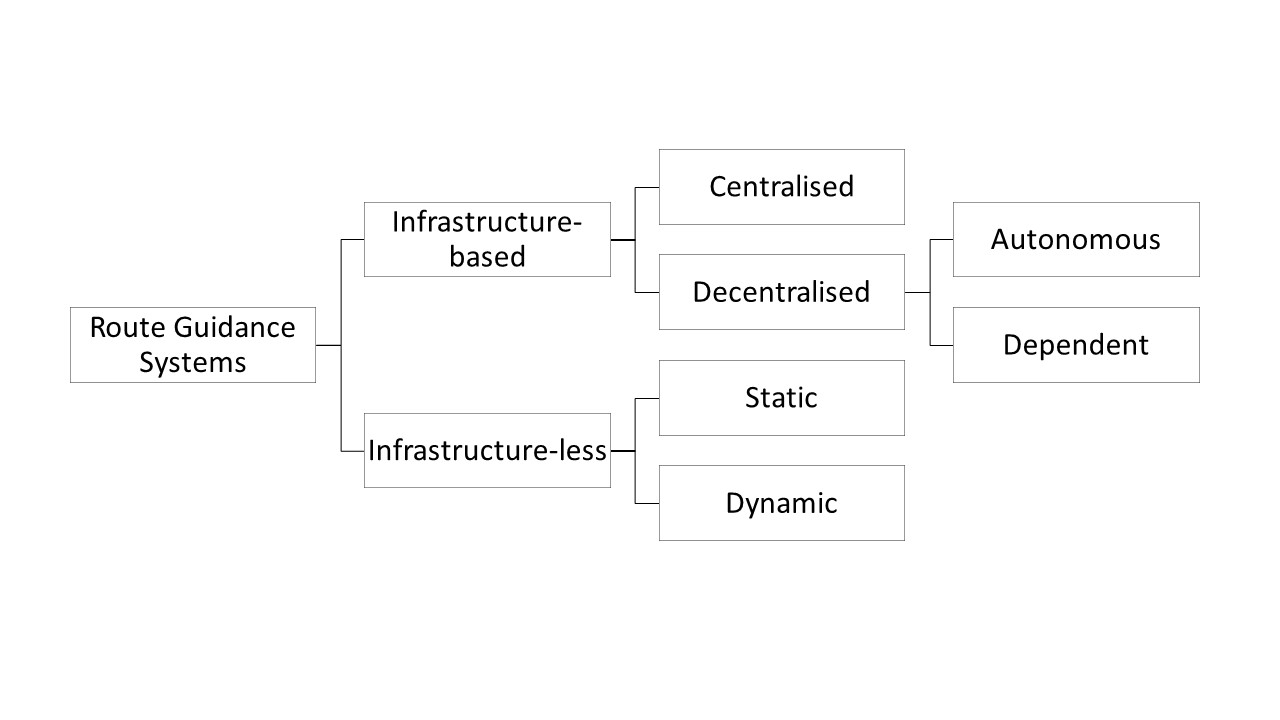
\includegraphics[width=0.55\linewidth]{image/DRS} \caption{Classification of route guidance systems (Khanjary and Hashemi, 2012)}\label{fig:unnamed-chunk-15}
\end{figure}

\textbf{Infrastructure-based architecture}
In both \emph{centralised-infrastructure based systems} and \emph{decentralised-infrastructure based systems} the data is, firstly, detected by traffic detection systems and then, collected and extracted by Traffic Message Channel (TMC). The difference is that, in \emph{centralised system} the optimal route information is calculated for the whole traffic network. On the other hand, in \emph{dependent decentralised system} the optimal route is calculated for each vehicle depending on its current location and destination. Further, in \emph{autonomous decentralised system} the data is collected by street nodes deployed over traffic network which then extract useful information for all surrounding streets and exchange the traffic information between one another. This allows each node to calculate the optimal routes for different destinations. The information about optimal routes can be received by vehicles, mobile phones or variable message signs (Khanjary and Hashemi, 2012).

\textbf{Infrastructure-less architecture}
\emph{Infrastructure-less decentralised static system} is one of the earliest developments. The database with traffic network map is available on mobile phone or as an in-vehicle unit where the optimal route is calculated based on a static information such as the shortest path. Further, in \emph{decentralised dynamic system}, vehicles (or mobile phones) are used to detect traffic data. They exchange the information with one another via infrastructure-less protocol such as the inter-vehicle communication or peer to peer. This results in vehicles having a real-time traffic information about the whole traffic network which enables them to calculate the optimal route based on a destination and current position of the vehicle. Importantly, the accuracy of the dynamic system depends on the volume of vehicles (or mobile devices) that serve as a traffic data sensors. The more vehicles are present, more information can be exchanged and the data is more reliable (Khanjary and Hashemi, 2012).

\hypertarget{key-stakeholders-13}{%
\subsection*{Key stakeholders}\label{key-stakeholders-13}}
\addcontentsline{toc}{subsection}{Key stakeholders}

\begin{itemize}
\tightlist
\item
  \textbf{Affected}: Drivers
\item
  \textbf{Responsible}: Local governments, Local or national road infrastructure provides, car manufacturers
\end{itemize}

\hypertarget{current-state-of-art-in-research-13}{%
\subsection*{Current state of art in research}\label{current-state-of-art-in-research-13}}
\addcontentsline{toc}{subsection}{Current state of art in research}

DRG is already a mature technology, hence the majority of the research focuses on the improvement of different aspects or its application in novel contexts. For example, a study conducted by Liang and Wakahara (2014) presents urban traffic predictions models in order to create a centralized proactive Route Guidance System. Results showed that models decreased the prediction error and reduced the travel time. Moreover, Wang and Niu (2019) in their research proposed simulation-based Distributed Dynamic Route Guidance System (DDRGS) based on the usage of data collection and communication techniques in Cooperative Vehicle-Infrastructure Systems (CVIS) and they stated that created DDRGS might be used in the CVIS. Lastly, Deflorio (2003) assessed the performance of strategy, which controls DRG systems during experiments in condition of quick growth of traffic. Eventually, Deflorio (2003) stated, among other conclusions, that the average travel time of DRG users was shorter than non-user ones in every examined case. Furthermore, a large body of research focuses on the use of DRG in the context of automated vehicles. For example, a study by Lazar et al.~(2019) employs deep reinforcement learning approach to decrease the congestion in mixed autonomous traffic. Furthermore, Kaminski et al.~(2020) investigates the effect of change in penetration level of smart cars on system characteristics including travel time in the environment where smart cars as well as human driven cars are both present. Importantly, smart cars are assumed to respond to changes in currently observed traffic by rerouting while traditional cars rely on historical information only. The results show that smart car rerouting algorithm reduced the total travel time by up to 30 \%.

\hypertarget{current-state-of-art-in-practice-13}{%
\subsection*{Current state of art in practice}\label{current-state-of-art-in-practice-13}}
\addcontentsline{toc}{subsection}{Current state of art in practice}

Nowadays, drivers of different brands of cars are using the Dynamic Route Guidance System already within the dynamic navigation in the car setup. Seat (2012) provides this function within the Navi satellite navigation software. Seat states in its manual for cars' owners that dynamic route guide is based on the TMC report and broadcasting channels are responsible for this feature (Media System Plus/ Navi System Owner's manual, 2012). Similar technology is used by Volkswagen (Volkswagen, 2021). Nonetheless, one of the most popular route guiding tools is Google Maps, which provides dynamic mapping, using real-time data from diverse channels to keep maps as updated as possible (Custom Maps \textbar{} Google Maps Platform \textbar{} Google Cloud, 2021). The range of features offered by Google Maps grows continuously. Recently, a `Finding a parking space' functionality was introduced, beyond plain dynamic route guidance (Vielmeier, 2019). Moreover, dynamic route planning plays an important role in commercial transport and urban deliveries (PTVGroup.com, 2021)

\hypertarget{relevant-initiatives-in-austria-13}{%
\subsection*{Relevant initiatives in Austria}\label{relevant-initiatives-in-austria-13}}
\addcontentsline{toc}{subsection}{Relevant initiatives in Austria}

\begin{itemize}
\tightlist
\item
  \href{https://www.volkswagen.at/technik-lexikon/navigationssystem}{Volkswagen}
\item
  \href{https://blog.ptvgroup.com/de/stadt-und-mobilitaet/routing-engine-hyperpath/}{PTVGroup}
\item
  \href{https://www.capterra.at/directory/30944/route-planning/software}{Capterra.at}
\end{itemize}

\hypertarget{impacts-with-respect-to-sustainable-development-goals-sdgs-13}{%
\subsection*{Impacts with respect to Sustainable Development Goals (SDGs)}\label{impacts-with-respect-to-sustainable-development-goals-sdgs-13}}
\addcontentsline{toc}{subsection}{Impacts with respect to Sustainable Development Goals (SDGs)}

\begin{longtable}[]{@{}
  >{\centering\arraybackslash}p{(\columnwidth - 8\tabcolsep) * \real{0.2029}}
  >{\centering\arraybackslash}p{(\columnwidth - 8\tabcolsep) * \real{0.1884}}
  >{\centering\arraybackslash}p{(\columnwidth - 8\tabcolsep) * \real{0.2029}}
  >{\centering\arraybackslash}p{(\columnwidth - 8\tabcolsep) * \real{0.2029}}
  >{\centering\arraybackslash}p{(\columnwidth - 8\tabcolsep) * \real{0.2029}}@{}}
\toprule()
\begin{minipage}[b]{\linewidth}\centering
Impact level
\end{minipage} & \begin{minipage}[b]{\linewidth}\centering
Indicator
\end{minipage} & \begin{minipage}[b]{\linewidth}\centering
Impact direction
\end{minipage} & \begin{minipage}[b]{\linewidth}\centering
Goal description and number
\end{minipage} & \begin{minipage}[b]{\linewidth}\centering
Source
\end{minipage} \\
\midrule()
\endhead
Individual & Reduced travel time & \textbf{+} & Sustainable economic development (\emph{8,11}) & Deflorio, 2003 \\
Systemic & Reduced accident risk due to route switching & \textbf{+} & Health \& Wellbeing (\emph{3}) & Chatterjee and McDonald, 1999 \\
\bottomrule()
\end{longtable}

\hypertarget{technology-and-societal-readiness-level-13}{%
\subsection*{Technology and societal readiness level}\label{technology-and-societal-readiness-level-13}}
\addcontentsline{toc}{subsection}{Technology and societal readiness level}

\begin{longtable}[]{@{}cc@{}}
\toprule()
TRL & SRL \\
\midrule()
\endhead
7-9 & 8-9 \\
\bottomrule()
\end{longtable}

\hypertarget{open-questions-13}{%
\subsection*{Open questions}\label{open-questions-13}}
\addcontentsline{toc}{subsection}{Open questions}

\begin{enumerate}
\def\labelenumi{\arabic{enumi}.}
\tightlist
\item
  How to increase time accuracy and generally, to improve performance of Dynamic Route Guidance through Traffic Message Channels?
\item
  Does and if yes, then to what degree Dynamic Route Guidance has an impact on the safety of drivers'?
\item
  What are the limitations and what risks could be possibly done through Dynamic Route Guidance?
\item
  What is the applicability of DRG for automated vehicles?
\end{enumerate}

\hypertarget{further-links-11}{%
\subsection*{Further links}\label{further-links-11}}
\addcontentsline{toc}{subsection}{Further links}

\begin{itemize}
\tightlist
\item
  \href{https://www.verizonconnect.com/at/industrie/vertriebsroutenplaner/}{Verizonconnect.com}
\end{itemize}

\hypertarget{references-13}{%
\subsection*{References}\label{references-13}}
\addcontentsline{toc}{subsection}{References}

\begin{itemize}
\tightlist
\item
  Chatterjee, K. and McDonald, M., (1999). THE NETWORK SAFETY EFFECTS OF DYNAMIC ROUTE GUIDANCE. ITS Journal - Intelligent Transportation Systems Journal, 4(3-4), pp.258-260.
\item
  Blischke, F., \& Hessing, B. (1998). Dynamic Route Guidance - Different Approaches to the System Concepts. SAE Transactions, 107, 1107-1111. Available at: \url{http://www.jstor.org/stable/44741041} {[}Accessed: 22 July 2021{]}
\item
  Deflorio, F., (2003). Evaluation of a reactive dynamic route guidance strategy. Transportation Research Part C: Emerging Technologies, 11(5), pp.375-388.
\item
  European Commission. (2021). Traveller Information - Mobility and Transport - European Commission. Available at: \url{https://ec.europa.eu/transport/themes/its/road/application_areas/traveller_information_es} {[}Accessed: 23 July 2021{]}.
\item
  Fan, Y., Lu, D., Li, Y. and Jiang, F., (2010). Design scheme of Distributed Dynamic Route Guidance System. 2010 2nd International Conference on Education Technology and Computer.
\item
  Google Cloud. (2021). Custom Maps \textbar{} Google Maps Platform \textbar{} Google Cloud. Available at: \url{https://cloud.google.com/maps-platform/maps} {[}Accessed: 23 July 2021{]}.
\item
  Kamiński, B., Kraiński, Ł., Mashatan, A., Prałat, P., \& Szufel, P. (2020). Multiagent Routing Simulation with Partial Smart Vehicles Penetration. Journal of Advanced Transportation, 2020.
\item
  Khanjary, M., \& Hashemi, S. M. (2012, May). Route guidance systems: Review and classification. In 2012 6th Euro American Conference on Telematics and Information Systems (EATIS) (pp.~1-7). IEEE.
\item
  Lazar, D. A., Bıyık, E., Sadigh, D., \& Pedarsani, R. (2021). Learning how to dynamically route autonomous vehicles on shared roads. Transportation Research Part C: Emerging Technologies, 130, 103258.
\item
  Liang, Z. and Wakahara, Y., (2014). Real-time urban traffic amount prediction models for dynamic route guidance systems. EURASIP Journal on Wireless Communications and Networking, 2014(1).
\item
  Media System Plus. (2012). Media System Plus/ Navi System Owner's manual. Available at: \url{https://www.firstforseatcars.com/downloads/multimedia/media-system-plus-navi-system-owners-manual.pdf} {[}Accessed: 22 July 2021{]}.
\item
  Mobility and transport. (2021). Intelligent transport systems Traveller Information. Available at: \url{https://ec.europa.eu/transport/themes/its/road/application_areas/traveller_information_es} {[}Accessed: 22 July 2021{]}.
\item
  Park, D., Kim, H., Lee, C. and Lee, K., (2009). Location-based dynamic route guidance system of Korea: System design, algorithms and initial results. KSCE Journal of Civil Engineering, 14(1), pp.51-59.
\item
  PTVGroup.com (2021). PTV Map\&Guide - der weltweit führende Lkw Routenplaner mit Transportkosten- und Mautrechner. Available at: \url{https://www.ptvgroup.com/de/loesungen/produkte/ptv-mapandguide/} {[}Accessed: 28 JUly 2021{]}
\item
  Seat.com. (2021). Dynamic Route Guidance - Car Terms \textbar{} SEAT. Available at: \url{https://www.seat.com/car-terms/d/dynaminc-route-guidance.html} {[}Accessed: 23 July 2021{]}.
\item
  Wang, J. and Niu, H., (2019). A distributed dynamic route guidance approach based on short-term forecasts in cooperative infrastructure-vehicle systems. Transportation Research Part D: Transport and Environment, 66, pp.23-34.
\item
  Vielmeier J. (2019). Google Maps als Navi verwenden: Das müsst ihr beachten. Available at: \url{https://trendblog.euronics.de/mobile-web/google-maps-als-navi-verwenden-das-muesst-ihr-beachten-61614/}. {[}Accessed: 28 July 2021{]}
\item
  Volkswagen.at (2021) Navigation. Volkswagen Technik-Highlights. Available at: \url{https://www.volkswagen.at/technik-lexikon/navigationssystem} {[}Accessed: 28 July 2021{]}.
\end{itemize}

\hypertarget{variable_speed}{%
\section{Variable speed limits and dynamic signage system}\label{variable_speed}}

\hypertarget{synonyms-13}{%
\subsection*{Synonyms}\label{synonyms-13}}
\addcontentsline{toc}{subsection}{Synonyms}

\emph{Variable speed limits (VSL), dynamic speed limits (DSL), Verkehrsbeeinflussungsanlagen (VBA), Changeable Message Signs (CMS), Dynamic Signage System}

\hypertarget{definition-14}{%
\subsection*{Definition}\label{definition-14}}
\addcontentsline{toc}{subsection}{Definition}

Speed limits are based on safety, mobility and environmental considerations. While fixed speed limits represent the appropriate speed for average conditions, variable or dynamic speed limits (DSL) take account of the real time traffic, or the road and weather conditions. Therefore, the latter reflect the safe speed better (Mobility and Transport, 2020). The road users are typically informed of the current speed limit by electronic signs above or beside the lanes (De Pauw et al., 2018), as shown in figure 1. These can be supplemented with warning signs (dynamic signage system). For example, if the usual speed limit is 100 km/h, the DSL could change to 80 km/h and further to 60 km/h, to limit rear-end collisions, if there is e.g., a traffic jam ahead or weather conditions are difficult.

\begin{figure}
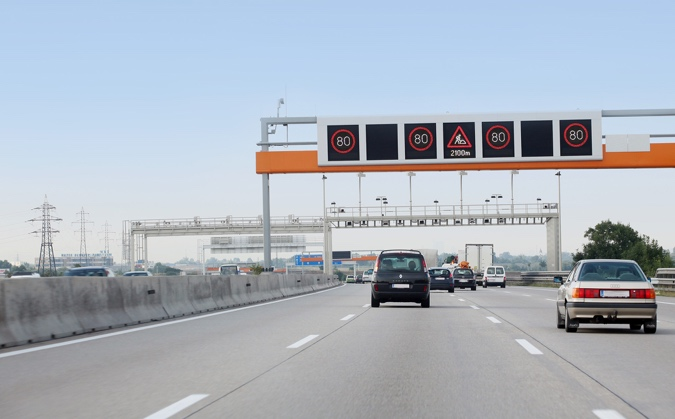
\includegraphics[width=0.9\linewidth]{image/dynamic_signage} \caption{Dynamic signage system in Austria (ASFiNAG, 2019b)}\label{fig:unnamed-chunk-18}
\end{figure}

With respect to the impact on the societal level, a Belgian study, by E. De Pauw et al.~showed a significant decrease (-18 \%) in the number of injury crashes after the introduction of a DSL system (De Pauw et al., 2018). F.G. Habtemichael and L. de Picado Santos (2013) found that a DSL system has the highest safety benefit during highly congested traffic conditions. The operational benefit in turn was the highest during lightly congested traffic conditions. However, the success of DSL is highly dependent on the level of driver compliance (Habtemichael \& de Picado Santos, 2013). Besides the safety aspects, the goal of DSL is to harmonize the traffic flow. Heavy traffic can cause shock waves, which result in longer travel times and large variations in the speeds of the vehicles. The latter again may lead to unsafe situations. By using DSL this phenomenon could be reduced (Hegyi et al., 2005). Traffic flow efficiency can be improved more, when DSL is combined with coordinated ramp metering (Carlson, 2010). Speed limits can also be temporary lowered, due to high emission values. If the emission values combined with the amount of traffic, reach a specific level, the DSL-System responds automatically and lowers the speed limit for a certain time. How high that level is, depends on the local policies (ASFiNAG, 2019c).

\hypertarget{key-stakeholders-14}{%
\subsection*{Key stakeholders}\label{key-stakeholders-14}}
\addcontentsline{toc}{subsection}{Key stakeholders}

\begin{itemize}
\tightlist
\item
  \textbf{Affected}: Motorways users, Drivers
\item
  \textbf{Responsible}: Motorway Infrastructure Agencies, Technology Providers, Policymakers, State authorities
\end{itemize}

\hypertarget{current-state-of-art-in-research-14}{%
\subsection*{Current state of art in research}\label{current-state-of-art-in-research-14}}
\addcontentsline{toc}{subsection}{Current state of art in research}

Studies show, that in retrospect most DSL implementations in Europe were efficient traffic safety and flow improvement. In the United States the increase in safety was significant as well, but the flow improvement was controversial (Lu \& Shladover, 2014). Hassan et al.~(2012) discovered that during bad weather conditions the combination of Changeable Message Signs (CMS) and DSL was the best way to improve safety. Current research shows that the benefits of DSL systems could be improved by integrating it in a fully connected vehicles (CV) environment (Wu et al., 2020). Currently, research focuses on the integration of C-ITS, to connect the infrastructure to the vehicles. European standards should be developed during the next years (Erhart, 2019).

\hypertarget{current-state-of-art-in-practice-14}{%
\subsection*{Current state of art in practice}\label{current-state-of-art-in-practice-14}}
\addcontentsline{toc}{subsection}{Current state of art in practice}

DSL systems are implemented and used around the world. The used algorithms differ, however. DSL integrated with C-ITS has been implemented in a test environment (Erhart, 2019).
Austrian motorways are managed by the ASFiNAG - currently they have 17 DSL systems in use. That means that about 19 \% of the Austrian Motorway-System are currently equipped by an DSL system (ASFiNAG, 2019a). So, there is potential for expansion. One global player in traffic management is the Austrian company Kapsch TrafficCom. Worldwide they have implemented their systems on more than 3.500 km of motorway (Kapsch TrefficCom). Kapsch TrafficCom's approximately 5,000 employees generated revenues of EUR 738 million in the fiscal year 2018/19.

\hypertarget{relevant-initiatives-in-austria-14}{%
\subsection*{Relevant initiatives in Austria}\label{relevant-initiatives-in-austria-14}}
\addcontentsline{toc}{subsection}{Relevant initiatives in Austria}

\begin{itemize}
\tightlist
\item
  \href{https://www.asfinag.at/verkehrssicherheit/verkehrsmanagement/verkehrssteuerung/}{Asfinag}
\item
  \href{https://blog.asfinag.at/technik-innovation/c-its-vernetzte-autos-intelligenter-verkehr/}{Asifinag blog}
\item
  \href{https://www.kapsch.net/ktc/Portfolio/IMS/Congestion/Highway-Traffic-Management}{kapsch.net}
\item
  \href{https://www.strabag-iss.com/databases/internet/_public/content30.nsf/web30?Openagent\&id=DE-STRABAGISS-DE_verkehrstechnik.html\&men1=3\&men2=5\&sid=351}{strabag-iss.com}
\item
  \href{https://www.pke.at/index.php?id=17\#c117}{pke.at}
\item
  \href{http://www.aigner-stahlbau.at/leistungen/verkehrstechnik/}{aigner-stahlbau.at}
\end{itemize}

\hypertarget{impacts-with-respect-to-sustainable-development-goals-sdgs-14}{%
\subsection*{Impacts with respect to Sustainable Development Goals (SDGs)}\label{impacts-with-respect-to-sustainable-development-goals-sdgs-14}}
\addcontentsline{toc}{subsection}{Impacts with respect to Sustainable Development Goals (SDGs)}

\begin{longtable}[]{@{}
  >{\centering\arraybackslash}p{(\columnwidth - 8\tabcolsep) * \real{0.2029}}
  >{\centering\arraybackslash}p{(\columnwidth - 8\tabcolsep) * \real{0.1884}}
  >{\centering\arraybackslash}p{(\columnwidth - 8\tabcolsep) * \real{0.2029}}
  >{\centering\arraybackslash}p{(\columnwidth - 8\tabcolsep) * \real{0.2029}}
  >{\centering\arraybackslash}p{(\columnwidth - 8\tabcolsep) * \real{0.2029}}@{}}
\toprule()
\begin{minipage}[b]{\linewidth}\centering
Impact level
\end{minipage} & \begin{minipage}[b]{\linewidth}\centering
Indicator
\end{minipage} & \begin{minipage}[b]{\linewidth}\centering
Impact direction
\end{minipage} & \begin{minipage}[b]{\linewidth}\centering
Goal description and number
\end{minipage} & \begin{minipage}[b]{\linewidth}\centering
Source
\end{minipage} \\
\midrule()
\endhead
Individual & Fatal collisions reduced & \textbf{+} & Health \& Wellbeing (\emph{3}) & Hegyi et al., 2005 \\
Individual & Travel time reduced & \textbf{+} & Sustainable economic development (\emph{8,11}) & Habtemichael \& de Picado Santos, 2013 \\
Systemic & Fatal collisions reduced & \textbf{+} & Health \& Wellbeing (\emph{3}) & Hegyi et al., 2005 \\
Systemic & Annual greenhouse gas emissions decrease & \textbf{+} & Environmental sustainability (\emph{7,12-13,15}) & Schimany, 2011 \\
\bottomrule()
\end{longtable}

\hypertarget{technology-and-societal-readiness-level-14}{%
\subsection*{Technology and societal readiness level}\label{technology-and-societal-readiness-level-14}}
\addcontentsline{toc}{subsection}{Technology and societal readiness level}

\begin{longtable}[]{@{}cc@{}}
\toprule()
TRL & SRL \\
\midrule()
\endhead
7-9 & 8-9 \\
\bottomrule()
\end{longtable}

\hypertarget{open-questions-14}{%
\subsection*{Open questions}\label{open-questions-14}}
\addcontentsline{toc}{subsection}{Open questions}

\begin{enumerate}
\def\labelenumi{\arabic{enumi}.}
\tightlist
\item
  Which algorithms for DSL are the most efficient ones?
\item
  How can DSL be further developed?
\item
  How can fail-safe operation be improved?
\item
  How can DSL be combined with C-ITS?
\end{enumerate}

\hypertarget{references-14}{%
\subsection*{References}\label{references-14}}
\addcontentsline{toc}{subsection}{References}

\begin{itemize}
\tightlist
\item
  ASFiNAG. (2019a). Handlungsfelder. Available at: \url{http://verkehrssicherheit.asfinag.at/aktionsprogramme/handlungsfelder/} {[}Accessed: 17 December 2020{]}.
\item
  ASFiNAG. (2019b). Verkehrsbeeinflussungsanlagen -- Für mehr Sicherheit: Arten von Verkehrsbeeinflussungsanlagen. Available at: \url{https://asfinag.azureedge.net/media/1607/vba-fotomontage.jpg} {[}Accessed: 11 December 2020{]}.
\item
  ASFiNAG. (2019c). Verkehrsbeeinflussungsanlagen -- Für mehr Sicherheit: Die VBA und der ``Lufthunderter''. Available at: \url{https://www.asfinag.at/verkehrssicherheit/verkehrsmanagement/verkehrssteuerung/} {[}Accessed: 3 December 2020{]}.
\item
  Carlson, R. C., Papamichail, I., Papageorgiou, M., \& Messmer, A. (2010). Optimal motorway traffic flow control involving variable speed limits and ramp metering. Transportation Science, 44(2), 238-253.
\item
  De Pauw, E., Daniels, S., Franckx, L., \& Mayeres, I. (2018). Safety effects of dynamic speed limits on motorways. Accident Analysis \& Prevention, 114, 83-89.
\item
  Erhart, Jaqueline. (2019). Vernetzte Autos, intelligenter Verkehr: Was C-ITS ist, was es kann und wem es nutzt. Available at: \url{https://blog.asfinag.at/technik-innovation/c-its-vernetzte-autos-intelligenter-verkehr/} {[}Accessed: 17 December 2020{]}.
\item
  Habtemichael, F. G., \& de Picado Santos, L. (2013). Safety and Operational Benefits of Variable Speed Limits under Different Traffic Conditions and Driver Compliance Levels. Transportation Research Record, 2386(1), 7--15. \url{https://doi.org/10.3141/2386-02}
\item
  Hassan, H. M., Abdel-Aty, M. A., Choi, K., \& Algadhi, S. A. (2012). Driver behavior and preferences for changeable message signs and variable speed limits in reduced visibility conditions. Journal of Intelligent Transportation Systems, 16(3), 132-146.
\item
  Hegyi, A., De Schutter, B., \& Hellendoorn, J. (2005). Optimal coordination of variable speed limits to suppress shock waves. IEEE Transactions on intelligent transportation systems, 6(1), 102-112.
\item
  Kapsch TrefficCom. Verkehrsmanagement auf Autobahnen. Available at: \url{https://www.kapsch.net/ktc/Portfolio/IMS/Congestion/Highway-Traffic-Management}
\item
  Lu, X.-Y., \& Shladover, S. E. (2014). Review of Variable Speed Limits and Advisories: Theory, Algorithms, and Practice. Transportation Research Record, 2423(1), 15--23. \url{https://doi.org/10.3141/2423-03} {[}Accessed: 8 January 2021{]}
\item
  Mobility and Transport \textbar{} European Commission. (2020). Dynamic speed limits. Available at: 2nd December 2020, from \url{https://ec.europa.eu/transport/road_safety/specialist/knowledge/speed/new_technologies_new_opportunities/dynamic_speed_limits_en} {[}Accessed: 2 December 2020{]}.
\item
  Schimany, H. K. (2011). Blue Globe Foresight.
\item
  Wu, Y., Abdel-Aty, M., Wang, L., \& Rahman, M. S. (2020). Combined connected vehicles and variable speed limit strategies to reduce rear-end crash risk under fog conditions. Journal of Intelligent Transportation Systems, 24(5), 494-513.
\end{itemize}

\hypertarget{adaptive_traffic_control}{%
\section{Smart traffic signal control}\label{adaptive_traffic_control}}

\hypertarget{synonyms-14}{%
\subsection*{Synonyms}\label{synonyms-14}}
\addcontentsline{toc}{subsection}{Synonyms}

\emph{Smart Traffic Lights, Adaptive Traffic Signal Control (ATSC), Traffic Signal Timing (TST), Traffic Signal Control (TSC)}

\hypertarget{definition-15}{%
\subsection*{Definition}\label{definition-15}}
\addcontentsline{toc}{subsection}{Definition}

In the recent years, the increasing population and the urgent need for efficient transport have led to severe traffic problems, especially in urban areas. Congestion mitigation solutions such as optimising the road network and improving basic urban management facilities have been proposed to cope with the pressure caused by the large traffic flow during peak hours. Among all possible methods, the adaptive traffic signal control (ATSC) which combine the intelligence into traffic light control systems has proven to be both, economical and efficient in relieving traffic pressure at congested intersections. With the development of deep learning techniques, ATSC strategies have shown great potential in integrating state-of-the-art intelligent methods (Wang et al., 2021).
Existing traffic light control systems either employ fixed programs without incorporating real-time traffic or take little account of traffic (Casas, 2017). They either set the traffic lights to the same duration every cycle or vary the duration depending on historical information. Some of them take input information from the underground sensors, such as inductive loop detectors, to detect vehicles near the traffic lights. However, such data is processed very crudely to determine the duration of green and red traffic lights. Consequently, they work in some cases (with low efficiency); however, during events such as sports, festivals, weather conditions or a typical high traffic volume scenario, the existing control systems tend to be paralysed.
The recent research paper by Liang et al., 2019 reports that an experienced police officer can efficiently and directly control the intersection by waving signals. Especially, in high traffic volume scenarios, a human operator observes the real-time traffic condition at the intersecting streets and adjusts the duration of the passage time accordingly. The aim of the adaptive traffic signal control is to provide flexibility and efficiency in traffic management comparable to that provided by a human operator through the employment of V2X and Deep Reinforcement learning (Wang et al., 2021).

\hypertarget{key-stakeholders-15}{%
\subsection*{Key stakeholders}\label{key-stakeholders-15}}
\addcontentsline{toc}{subsection}{Key stakeholders}

\begin{itemize}
\tightlist
\item
  \textbf{Affected}: Road drivers, cyclists, pedestrians
\item
  \textbf{Responsible}: Local governments, Local or national road infrastructure provides, car manufacturers
\end{itemize}

\hypertarget{current-state-of-art-in-research-15}{%
\subsection*{Current state of art in research}\label{current-state-of-art-in-research-15}}
\addcontentsline{toc}{subsection}{Current state of art in research}

Existing ATSC methods focus on varying the duration of green or red cycles based on real-time information. Nevertheless, this approach is not optimal because it neglects the impact of the current green and red lights durations on the upcoming traffic. Therefore, ATSC performs better than the fixed duration system but worse than more flexible methods because the optimal phase duration in the last cycles does not perform better in the future considering updated information about complex traffic conditions.

With Deep Learning (DL) methods (which serve as input to the intersection controls), the optimal design of the basic control indices such as green phase duration and phase sequence of the traffic light at an intersection can be considered as an optimal decision-making procedure. Next, the reinforcement learning (RL) is applied to signal control to obtain the best control procedure for a signalised intersection. However, in order to achieve instantaneous data acquisition and transmission with low latency, Cooperative Vehicle Infrastructure System (CVIS) is needed to support inter-vehicle communication and vehicles with roadside infrastructure communication (see \protect\hyperlink{v2x}{V2X section}). Compared to traditional sensor detectors, V2X can collect more accurate traffic data to provide comprehensive information for traffic control, resulting in better RL decision-making (Wang et al., 2021).
Moreover, the analysis of the recent literature for the optimisation of TSC systems, which have been published from January 2015 to January 2020 revealed that only two papers deal with signalised roundabouts. Roundabouts have different traffic dynamics compared to regular intersections. With an increasing use of signalised roundabouts, especially in urban areas, it is believed that TSC for signalised roundabouts is a particular research gap in this area. Although there are studies conducted using real data and real-time control, there are scarce results and/or methods applied or adapted in real life. One of the main challenges for researchers in this field would be to bring these methods to decision makers and implementers.
Moreover, a vast majority of work found on this topic deals with the timing of traffic signals and their impact on average delay and/or emissions. An important part of busy intersections, especially in metropolitan areas, is pedestrian traffic. With the exception of Vilarinho et al., (2017) and Yu et al., (2017), pedestrians and the effects of their behaviour are not modelled in the studies. The same applies for drivers' behaviour. An important research direction would be to analyse the effects of pedestrian and driver behaviour on the models.
Furthermore, the number of studies dealing with autonomous vehicles and technologies is growing rapidly. The most recent studies address the general area of how autonomous vehicles can be introduced safely and/or efficiently and/or environmentally friendly into the traffic flow
(Qadri et al., 2020a).
While learning from trial and error is the key idea in RL, the learning cost of RL for complicated problems might be unacceptable. Therefore, how to learn efficiently (e.g.~from limited data samples, efficient exploration, transfer of learned knowledge) is a critical issue for the application of RL in traffic signal control (Wei et al., 2019).

\hypertarget{current-state-of-art-in-practice-15}{%
\subsection*{Current state of art in practice}\label{current-state-of-art-in-practice-15}}
\addcontentsline{toc}{subsection}{Current state of art in practice}

A number of stakeholders are focusing on the development of adaptive traffic control systems that support a range of smart city traffic applications, such as public transport signal priority (see \protect\hyperlink{public_trans_priority}{PTSP section} for further details), eco-driving support, messaging, intelligent traffic signal control (STSC) and emergency vehicle signal pre-emption (EVSP). Due to these factors and steady advances in sensors, artificial intelligence (AI) and machine learning, the global market for adaptive traffic control systems is forecasted to reach the market value of US\$21.9 billion by the end of 2030.
Governments and city administrations in different regions of the world are looking for new ways to respond to the increasing number of traffic accidents and managing road congestion, which is why adaptive traffic control systems have attracted a lot of interest in recent years as a viable alternative to address the existing challenges (The Sentinel Newspaper, 2021).
There are many options already existing and more are still under development. Currently available adaptive signal control technologies include:

\begin{itemize}
\tightlist
\item
  Split Cycle Offset Optimisation Technique (SCOOT);
\item
  Sydney Coordinated Adaptive Traffic System (SCATS),
\item
  Real Time Hierarchical Optimised Distributed Effective System (RHODES);
\item
  Optimised Policies for Adaptive Control (OPAC) \emph{Virtual Fixed Cycle}
\item
  ACS Lite
\end{itemize}

Real-time control of traffic systems has proven performance record, yet these systems have been deployed in less than 1\% of existing traffic signals in America. The Federal Highway Administration is now working to roll out these technologies to the rest of the country (Curtis, 2017). Further, for example, in Germany the adaptive signal control system has been installed on a 6 km long arterial in Muenster, where it was demonstrated to have positive effect on traffic quality and improve the bus transit by 30\% based on the adopted performance index (Brilon \& Wietholt, 2013).

\hypertarget{relevant-initiatives-in-austria-15}{%
\subsection*{Relevant initiatives in Austria}\label{relevant-initiatives-in-austria-15}}
\addcontentsline{toc}{subsection}{Relevant initiatives in Austria}

\begin{itemize}
\tightlist
\item
  \href{https://www.asfinag.at/road-safety/traffic-management/traffic-control/}{Asfinag}
\item
  \href{https://www.atc.or.at/smart-cities/smart-mobility/urban-traffic-management-solutions/}{ATC}
\end{itemize}

\hypertarget{impacts-with-respect-to-sustainable-development-goals-sdgs-15}{%
\subsection*{Impacts with respect to Sustainable Development Goals (SDGs)}\label{impacts-with-respect-to-sustainable-development-goals-sdgs-15}}
\addcontentsline{toc}{subsection}{Impacts with respect to Sustainable Development Goals (SDGs)}

\begin{longtable}[]{@{}
  >{\centering\arraybackslash}p{(\columnwidth - 8\tabcolsep) * \real{0.2029}}
  >{\centering\arraybackslash}p{(\columnwidth - 8\tabcolsep) * \real{0.1884}}
  >{\centering\arraybackslash}p{(\columnwidth - 8\tabcolsep) * \real{0.2029}}
  >{\centering\arraybackslash}p{(\columnwidth - 8\tabcolsep) * \real{0.2029}}
  >{\centering\arraybackslash}p{(\columnwidth - 8\tabcolsep) * \real{0.2029}}@{}}
\toprule()
\begin{minipage}[b]{\linewidth}\centering
Impact level
\end{minipage} & \begin{minipage}[b]{\linewidth}\centering
Indicator
\end{minipage} & \begin{minipage}[b]{\linewidth}\centering
Impact direction
\end{minipage} & \begin{minipage}[b]{\linewidth}\centering
Goal description and number
\end{minipage} & \begin{minipage}[b]{\linewidth}\centering
Source
\end{minipage} \\
\midrule()
\endhead
Systemic & Scarcity of studies that include the effects of pedestrians behaviour & \textbf{-} & Equality (\emph{5,10}) & Qadri et al., 2020b \\
Systemic & Decrease in congestion at the intersections & \textbf{+} & Sustainable economic development (\emph{8,11}) & Wang et al., 2021 \\
Systemic & Progress in the use of RL algorithms and V2X technologies & \textbf{+} & Innovation \& Infrastructure (\emph{9}) & Wang et al., 2021 \\
\bottomrule()
\end{longtable}

\hypertarget{technology-and-societal-readiness-level-15}{%
\subsection*{Technology and societal readiness level}\label{technology-and-societal-readiness-level-15}}
\addcontentsline{toc}{subsection}{Technology and societal readiness level}

\begin{longtable}[]{@{}cc@{}}
\toprule()
TRL & SRL \\
\midrule()
\endhead
7-9 & 7-8 \\
\bottomrule()
\end{longtable}

\hypertarget{open-questions-15}{%
\subsection*{Open questions}\label{open-questions-15}}
\addcontentsline{toc}{subsection}{Open questions}

\begin{enumerate}
\def\labelenumi{\arabic{enumi}.}
\tightlist
\item
  How can ATSC for signalised roundabouts be designed, developed and implemented?
\item
  How can pedestrian movement be included to a larger extent into the algorithms of ATSC?
\item
  How can reinforcement learning algorithms learn efficiently from limited data samples for the purpose traffic signal control?
\end{enumerate}

\hypertarget{further-links-12}{%
\subsection*{Further links}\label{further-links-12}}
\addcontentsline{toc}{subsection}{Further links}

\begin{itemize}
\tightlist
\item
  \href{https://www.rapidflowtech.com/surtrac}{rapidflowtech.com}
\item
  \href{https://www.fhwa.dot.gov/innovation/everydaycounts/edc-1/asct.cfm}{fhwa.dot.gov}
\end{itemize}

\hypertarget{references-15}{%
\subsection*{References}\label{references-15}}
\addcontentsline{toc}{subsection}{References}

\begin{itemize}
\tightlist
\item
  Brilon, W., \& Wietholt, T. (2013). Experiences with adaptive signal control in Germany. Transportation research record, 2356(1), 9-16.
\item
  Casas, N. (2017). Deep deterministic policy gradient for urban traffic light control. ArXiv, 1--12.
\item
  Curtis, E. (2017, September 8). EDC-1: Adaptive Signal Control Technology \textbar{} Federal Highway Administration. \url{https://www.fhwa.dot.gov/innovation/everydaycounts/edc-1/asct.cfm}
\item
  Liang, X., Du, X., Wang, G., \& Han, Z. (2019). A Deep Reinforcement Learning Network for Traffic Light Cycle Control. IEEE Transactions on Vehicular Technology, 68(2), 1243--1253. \url{https://doi.org/10.1109/TVT.2018.2890726}
\item
  Qadri, S. S. S. M., Gökçe, M. A., \& Öner, E. (2020a). State-of-art review of traffic signal control methods: challenges and opportunities. European Transport Research Review, 12(1), 55. \url{https://doi.org/10.1186/s12544-020-00439-1}
\item
  Qadri, S. S. S. M., Gökçe, M. A., \& Öner, E. (2020b). State-of-art review of traffic signal control methods: challenges and opportunities. European Transport Research Review, 12(1), 1--23. \url{https://doi.org/10.1186/s12544-020-00439-1}
\item
  The Sentinel Newspaper. (2021, March 3). Adaptive Traffic Control System Market to reach US\$ 21.9 Bn by 2030 -- KSU \textbar{} The Sentinel Newspaper. \url{https://ksusentinel.com/2021/03/03/adaptive-traffic-control-system-market-to-reach-us-21-9-bn-by-2030/}
\item
  Vilarinho, C., Tavares, J. P., \& Rossetti, R. J. F. (2017). Intelligent Traffic Lights: Green Time Period Negotiaton. Transportation Research Procedia, 22, 325--334. \url{https://doi.org/https://doi.org/10.1016/j.trpro.2017.03.039}
\item
  Wang, T., Cao, J., \& Hussain, A. (2021). Adaptive Traffic Signal Control for large-scale scenario with Cooperative Group-based Multi-agent reinforcement learning. Transportation Research Part C: Emerging Technologies, 125(February), 103046. \url{https://doi.org/10.1016/j.trc.2021.103046}
\item
  Wei, H., Zheng, G., Gayah, V., \& Li, Z. (2019). A survey on traffic signal control methods. ArXiv, 1(1).
\item
  Yu, C., Ma, W., Han, K., \& Yang, X. (2017). Optimization of vehicle and pedestrian signals at isolated intersections. Transportation Research Part B: Methodological, 98, 135--153. \url{https://doi.org/https://doi.org/10.1016/j.trb.2016.12.015}
\end{itemize}

\hypertarget{p_g_fleet_management}{%
\section{Passengers and goods fleet management}\label{p_g_fleet_management}}

\hypertarget{definition-16}{%
\subsection*{Definition}\label{definition-16}}
\addcontentsline{toc}{subsection}{Definition}

According to Mixtelematics.com (2021) \emph{``Fleet management refers to the overall actions that take place to keep a fleet running efficiently, on time, and within budget. It can be defined as the processes used by fleet managers to monitor fleet activities and make decisions from asset management, dispatch, scheduling, routing, vehicle acquisition and disposal. It helps companies ensure compliance, improve efficiency, and reduce costs.''} It is claimed to apply to organisations and firms that use more than five vehicles. The main responsibilities of fleet managers are reducing costs, vehicle tracking and safety, driver's safety and retention, vehicle acquisition and electronic Logging Device (ELD) compliance (in case of the USA). On the other hand, the benefits of fleet management include the automation of manual tasks, increase in profitability, an improvement in fleet safety and customer service. Further, the major challenges that fleet managers face are fuel management, vehicle acquisition, optimisation of Vehicle performance, meeting compliance requirements, control of costs and health and safety (Mixtelematics.com, 2021).

Fleet management is present in a range of industries including public transport, emergency services, transport and distribution or rental and leasing of vehicles.

\textbf{Public transport}
Fleet management with respect to public transport focuses on the monitoring and management of drivers and vehicles to help public transport operators to improve performance and system capabilities. It can be achieved by real-time tracking of vehicles location and robust data collection. The passenger fleet management features include (Nec.com,2021):

\begin{itemize}
\tightlist
\item
  Real time passenger information system, where the key is an estimated arrival time (ETA) based on day, time, route type, schedule type, dwell time, travel time, etc (For more information see \protect\hyperlink{info_and_route_planning}{Multimodal information and route planning})
\item
  In-vehicle visual and audio passenger announcement system is defined for each route and stop providing real time information about the progress of the vehicle, any route disruptions and deviations
\item
  Real time data analysis and management monitors transit services including on route adherence and schedule monitoring as well as wait time monitoring
\item
  Routing and trip assignment schedules trips but it also allows for a dynamic trip assignment
\end{itemize}

\textbf{Transport and distribution}
In transportation industry implementation of fleet management through an on-board mobile technology can help in route optimisation, improved communication with drivers, management of fuel consumption and more efficient jobs assignment and scheduling. Furthermore, a special case of fleet management involves future fleets of AVs as described by Hyland \& Mahmassani (2017) who provide a comprehensive taxonomy for shared autonomous vehicle fleet management.

\hypertarget{key-stakeholders-16}{%
\subsection*{Key stakeholders}\label{key-stakeholders-16}}
\addcontentsline{toc}{subsection}{Key stakeholders}

\begin{itemize}
\tightlist
\item
  \textbf{Affected}: Commercial drivers, public transport drivers and managers, public transport passengers
\item
  \textbf{Responsible}: Public transport operators, Transportation companies, Vehicles manufacturers
\end{itemize}

\hypertarget{current-state-of-art-in-research-16}{%
\subsection*{Current state of art in research}\label{current-state-of-art-in-research-16}}
\addcontentsline{toc}{subsection}{Current state of art in research}

Research with respect to fleet management focuses on development and implementation of modern and holistic solutions using, for example, the Internet of Things (IoT). For instance, Killeen et al.~(2019) proposed the use of data produced by the IoT in fleet management context to improve predictive maintenance of fleets. Further, Nuhic et al.~(2018) developed a new battery health monitoring algorithm to increase the accuracy of battery degradation prediction. Next, Stancel \& Surugiu (2017) developed a system that monitors truck platoon in a real-time and provides information about the length of the route, travel time and fuel consumption. The system allows for computation of optimal routes with respect to fuel consumption.

\hypertarget{current-state-of-art-in-practice-16}{%
\subsection*{Current state of art in practice}\label{current-state-of-art-in-practice-16}}
\addcontentsline{toc}{subsection}{Current state of art in practice}

Currently, multiple technology-focused companies offer fleet management software all over the world such as \href{https://www.fleetio.com/}{Fleetio}, \href{https://www.samsara.com/at/}{Sesmara}, \href{https://gsmtasks.com/}{GSMtasks} or \href{https://www.avrios.com/?utm_source=capterra\&utm_medium=cpc\&utm_campaign=software-comparison}{Avrios}. There are also companies such as \href{https://www.urbantz.com/}{Urbantz} or \href{https://onfleet.com/}{OnFleet} that specialise in particular cases of the management of local, last mile green deliveries. Further, \href{https://gourban.co/}{Go Urban} offers technological solution for shared mobility fleets.

Moreover, between 2001 and 2004 the EU project F-MAN took place in several countries (Portugal, Spain, France, Italy, Austria, Czech Republic, Slovakia, Hungary, Slovenia and Romania) that aimed at exploration of advantages of the development of innovative tools that would allow taking a new approach to management of internationally operated fleets of freight wagons. The developed system consisted of three components (Cosulich et al., 2006):

\begin{itemize}
\tightlist
\item
  Tracking System Module (TSM), consists of on-board terminals which are located in the wagons and in the ground station
\item
  Data Processing Module (DPM), is a software app responsible for data exchange and maintenance
\item
  Asset Management Module (AMM), links the remaining modules, processes orders, selects and books wagons, organises trips and logs data for asset management purposes
\end{itemize}

The field tests showed that compared to other management systems, current system is between 40\% and 80\% more efficient.

The previous European projects were, among others, \href{https://ec.europa.eu/research/participants/documents/downloadPublic?documentIds=080166e5a7b1dc79\&appId=PPGMS}{CHINO} (2006-2009) that looked at the containers handling in intermodal nodes, \href{https://cordis.europa.eu/project/id/251589/reporting}{SAIL} (2011-2014) which explored ICT tools for logistics and business operations in the port and dry port areas or \href{http://www.mitproject.eu/}{MIT} (2004-2009) that was concerned with fully automated system for the distributed intermodal transport (Harris et al., 2006).

Finally, a technology company \href{https://www.nec.com/en/global/solutions/transportation/task/fms_pis.html}{Nec.com} provides smart fleet management system for 1700 buses in Hong-Kong as well as bus fleets in Singapore and India showing that these system can be applied in dense and complex urban networks and offer smart solutions that improve the performance of public transport.

\hypertarget{relevant-initiatives-in-austria-16}{%
\subsection*{Relevant initiatives in Austria}\label{relevant-initiatives-in-austria-16}}
\addcontentsline{toc}{subsection}{Relevant initiatives in Austria}

\begin{itemize}
\tightlist
\item
  \href{https://www.ait.ac.at/en/solutions/plan}{AIT}
\item
  \href{https://www.samsara.com/at/}{Sesmara}
\item
  \href{https://www.frotcom.com/de}{Frotcom}
\end{itemize}

\hypertarget{impacts-with-respect-to-sustainable-development-goals-sdgs-16}{%
\subsection*{Impacts with respect to Sustainable Development Goals (SDGs)}\label{impacts-with-respect-to-sustainable-development-goals-sdgs-16}}
\addcontentsline{toc}{subsection}{Impacts with respect to Sustainable Development Goals (SDGs)}

\begin{longtable}[]{@{}
  >{\centering\arraybackslash}p{(\columnwidth - 8\tabcolsep) * \real{0.2029}}
  >{\centering\arraybackslash}p{(\columnwidth - 8\tabcolsep) * \real{0.1884}}
  >{\centering\arraybackslash}p{(\columnwidth - 8\tabcolsep) * \real{0.2029}}
  >{\centering\arraybackslash}p{(\columnwidth - 8\tabcolsep) * \real{0.2029}}
  >{\centering\arraybackslash}p{(\columnwidth - 8\tabcolsep) * \real{0.2029}}@{}}
\toprule()
\begin{minipage}[b]{\linewidth}\centering
Impact level
\end{minipage} & \begin{minipage}[b]{\linewidth}\centering
Indicator
\end{minipage} & \begin{minipage}[b]{\linewidth}\centering
Impact direction
\end{minipage} & \begin{minipage}[b]{\linewidth}\centering
Goal description and number
\end{minipage} & \begin{minipage}[b]{\linewidth}\centering
Source
\end{minipage} \\
\midrule()
\endhead
Individual & Drivers safety increases & \textbf{+} & Health \& Wellbeing (\emph{3}) & Salazar-Cabrera et al., 2019 \\
Systemic & Optimised fuel consumption & \textbf{+} & Sustainable economic development (\emph{8,11}) & Stancel \& Surugiu, 2017 \\
Systemic & Continuous development of technologies for fleet management & \textbf{+} & Innovation \& Infrastructure (\emph{9}) & Xu et al., 2019 \\
\bottomrule()
\end{longtable}

\hypertarget{technology-and-societal-readiness-level-16}{%
\subsection*{Technology and societal readiness level}\label{technology-and-societal-readiness-level-16}}
\addcontentsline{toc}{subsection}{Technology and societal readiness level}

\begin{longtable}[]{@{}cc@{}}
\toprule()
TRL & SRL \\
\midrule()
\endhead
7-9 & 7-9 \\
\bottomrule()
\end{longtable}

\hypertarget{open-questions-16}{%
\subsection*{Open questions}\label{open-questions-16}}
\addcontentsline{toc}{subsection}{Open questions}

\begin{enumerate}
\def\labelenumi{\arabic{enumi}.}
\tightlist
\item
  How new technologies can alleviate the problem of managing geographically dispersed team?
\item
  How can an integration of fleet data into existing software systems be conducted smoothly?
\end{enumerate}

\hypertarget{further-links-13}{%
\subsection*{Further links}\label{further-links-13}}
\addcontentsline{toc}{subsection}{Further links}

\begin{itemize}
\tightlist
\item
  \href{https://www.nec.com/en/global/solutions/transportation/task/fms_pis.html}{Nec.com}
\item
  \href{https://fleet.randmcnally.com/field-service/passenger-transit}{Fleet.randmcnally.com}
\end{itemize}

\hypertarget{references-16}{%
\subsection*{References}\label{references-16}}
\addcontentsline{toc}{subsection}{References}

\begin{itemize}
\tightlist
\item
  Cosulich, G., Derito, A., Giannettoni, M., \& Savio, S. (2006). RESULTS OF THE EVALUATION OF F-MAN--AN INNOVATIVE SOLUTION FOR THE MANAGEMENT OF RAILWAY CARGO FLEETS. IFAC Proceedings Volumes, 39(12), 331-336.
\item
  Harris, I., Wang, Y., \& Wang, H. (2015). ICT in multimodal transport and technological trends: Unleashing potential for the future. International Journal of Production Economics, 159, 88-103.
\item
  Hyland, M. F., \& Mahmassani, H. S. (2017). Taxonomy of shared autonomous vehicle fleet management problems to inform future transportation mobility. Transportation Research Record, 2653(1), 26-34.
\item
  Killeen, P., Ding, B., Kiringa, I., \& Yeap, T. (2019). IoT-based predictive maintenance for fleet management. Procedia Computer Science, 151, 607-613.
\item
  Mixtelematics.com (2021). What Is Fleet Management? Available at: \url{https://www.mixtelematics.com/resources/what-is-fleet-management} {[}Accessed: 05/08/2021{]}
\item
  Nec.com (2021). What are Fleet Management Systems? Available at: \url{https://www.nec.com/en/global/solutions/transportation/task/fms_pis.html} {[}Accessed: 09/08/2021{]}
\item
  Nuhic, A., Bergdolt, J., Spier, B., Buchholz, M., \& Dietmayer, K. (2018). Battery health monitoring and degradation prognosis in fleet management systems. World Electric Vehicle Journal, 9(3), 39.
\item
  Salazar-Cabrera, R., De La Cruz, Á. P., \& Molina, J. M. M. (2019, March). Fleet management and control system from intelligent transportation systems perspective. In 2019 2nd Latin American Conference on Intelligent Transportation Systems (ITS LATAM) (pp.~1-7). IEEE.
\item
  Stancel, I. N., \& Surugiu, M. C. (2017). Fleet Management System for Truck Platoons-Generating an Optimum Route in Terms of Fuel Consumption. Procedia Engineering, 181, 861-867.
\item
  Xu, G., Li, M., Luo, L., Chen, C. H., \& Huang, G. Q. (2019). Cloud-based fleet management for prefabrication transportation. Enterprise Information Systems, 13(1), 87-106.
\end{itemize}

\hypertarget{urban_access}{%
\section{Urban access management}\label{urban_access}}

\hypertarget{synonyms-15}{%
\subsection*{Synonyms}\label{synonyms-15}}
\addcontentsline{toc}{subsection}{Synonyms}

\emph{Access Regulation Schemes (ARS), Urban Vehicle Access Regulations (UVARs), Low Emission Zones (LEZ), Access Restrictions, Traffic Restrictions, Limited Traffic Zones, Permit Schemes}

\hypertarget{definition-17}{%
\subsection*{Definition}\label{definition-17}}
\addcontentsline{toc}{subsection}{Definition}

Urban Access Management can be seen as regulations, restrictions or bans, for traffic entering cities. Factors like congestion, air pollution, traffic noise or damage to historic buildings are influencing the liveability of cities negatively. Therefore, many cities have been introducing Access Regulation Schemes (ARS) with the goal of less vehicles entering the particular city or area. Implementing a pedestrian zone, is the simplest type of ARS and can improve the attractiveness of tourist attractions or shopping streets significantly (Sadler Consultants Europe GmbH, n.d. c). ARS can be differentiated by vehicle type, vehicle weight, by type of trip (e.g.~delivery), by driver (e.g.~residents or access), or applies to all vehicles (Sadler Consultants Europe GmbH, n.d. c). Furthermore, ARS can be static or dynamic, depending, for example, on the time of the day or air pollution levels. A list below provides examples of current measures used in the urban areas:

\begin{itemize}
\tightlist
\item
  Low Emission Zones (LEZ)
\item
  Limited Access Zones
\item
  Urban Toll Schemes / Congestion Charging (CS)
\item
  Emergency Air Pollution Schemes
\item
  Zero Emission Zones (ZEZ)
\item
  Other Access Regulations (like Limited Traffic Zones, Through traffic bans, `Superblocks´ etc.)
\item
  Smaller Regulations / Restrictions (like school streets or shared spaces) (Sandler Consultants Europe GmbH, n.d. d).
\end{itemize}

Solutions for ARS can be enforced by physical barriers or cameras, based on automatic number plate recognition (ANPR) systems and/or dedicated short-range communication (DSRC) technology, using on-board units (OBUs) (Kapsch TrafficCom., n.d. b) or by police or local authority officers (Sadler Consultants Europe GmbH, n.d. c).

The impact of Urban Vehicle Access Regulations differs according the implemented schemes, but several common goals are addressed:

\begin{itemize}
\tightlist
\item
  Air quality improvement
\item
  Traffic congestion reduction
\item
  Urban landscape preservation (historical town centres)
\item
  Climate change mitigation
\item
  Quality of life
\item
  Noise mitigation
\item
  Road safety
\item
  Raising revenues (Sandler Consultants Europe GmbH, n.d. d).
\end{itemize}

In Austria, several cities and regions have implemented Low Emission Zones (LEZ) for lorries. For example, the city of Salzburg has Access Regulations (AR) for the city centre in place, so only vehicles with a specific reason (delivery or police) are allowed to enter. On the other hand, Tirol introduces occasionally traffic bans during the summer months (Sandler Consultants Europe GmbH, n.d. a). While, the city of Vienna aims at implementing a traffic-calmed city centre by 2022 (Stadt Wien, 2020).

\hypertarget{key-stakeholders-17}{%
\subsection*{Key stakeholders}\label{key-stakeholders-17}}
\addcontentsline{toc}{subsection}{Key stakeholders}

\begin{itemize}
\tightlist
\item
  \textbf{Affected}: Car Users -- especially users of old or high polluting cars, Truck drivers, Shippers/producers, Wholesalers, Logistics providers, Retailers, Consumers, Citizens, Authorities
\item
  \textbf{Responsible}: Municipalities, Road Operators, Urban Traffic Management, Authorities
\end{itemize}

\hypertarget{current-state-of-art-in-research-17}{%
\subsection*{Current state of art in research}\label{current-state-of-art-in-research-17}}
\addcontentsline{toc}{subsection}{Current state of art in research}

Current research addresses the evaluation of UVAR implementations and identifies their positive and negative effects. For example, Lopez (2018) found that Urban Consolidation Centres (UCCs), Cargo Bikes (CBs) and Off-hour Deliveries (OHDs) are the three preferred types of solutions to assist in mitigating unwanted side-effects of UVARs on the logistic sector. Further, current research focuses on the sustainable urban planning in cites affected by mass tourism (García Hernández, 2019; Nolasco‐Cirugeda, 2020). Additionally, most recent area of research deals with geofencing that aims at creating digital zones defined on a map, with specific rules, that can be transmitted to the vehicles (Arnesen et al., 2020).

\hypertarget{current-state-of-art-in-practice-17}{%
\subsection*{Current state of art in practice}\label{current-state-of-art-in-practice-17}}
\addcontentsline{toc}{subsection}{Current state of art in practice}

According to Lopez (2018) there are the two preferred UVAR schemes: Low Emission Zones (LEZ) and Congestion Charging (CC). The implementation of these schemes is widely spread within Europe but follows different approaches. Lopez (2018) identified two dominant LEZ enforcement models, first visual surveillance using windscreen stickers and second, cameras with ANPR technology. Furthermore it is argued that \emph{``It is very important to consider that the degree of impact of each measure not only varies from city to city but also depends on the presence of a mix of access regulations``} (Lopez, 2018).

\hypertarget{relevant-initiatives-in-austria-17}{%
\subsection*{Relevant initiatives in Austria}\label{relevant-initiatives-in-austria-17}}
\addcontentsline{toc}{subsection}{Relevant initiatives in Austria}

\begin{itemize}
\tightlist
\item
  \href{https://www.ris.bka.gv.at/GeltendeFassung.wxe?Abfrage=LrW\&Gesetzesnummer=20000270}{ris.bka.gv.at}
\item
  \href{https://www.wien.gv.at/ma22-lgb/luftgi.htm}{wien.gv.at}
\item
  \href{https://www.kapsch.net/ktc/its-solutions/urban-access-management/access-restriction/}{kapsch.net}
\end{itemize}

\hypertarget{impacts-with-respect-to-sustainable-development-goals-sdgs-17}{%
\subsection*{Impacts with respect to Sustainable Development Goals (SDGs)}\label{impacts-with-respect-to-sustainable-development-goals-sdgs-17}}
\addcontentsline{toc}{subsection}{Impacts with respect to Sustainable Development Goals (SDGs)}

\begin{longtable}[]{@{}
  >{\centering\arraybackslash}p{(\columnwidth - 8\tabcolsep) * \real{0.2029}}
  >{\centering\arraybackslash}p{(\columnwidth - 8\tabcolsep) * \real{0.1884}}
  >{\centering\arraybackslash}p{(\columnwidth - 8\tabcolsep) * \real{0.2029}}
  >{\centering\arraybackslash}p{(\columnwidth - 8\tabcolsep) * \real{0.2029}}
  >{\centering\arraybackslash}p{(\columnwidth - 8\tabcolsep) * \real{0.2029}}@{}}
\toprule()
\begin{minipage}[b]{\linewidth}\centering
Impact level
\end{minipage} & \begin{minipage}[b]{\linewidth}\centering
Indicator
\end{minipage} & \begin{minipage}[b]{\linewidth}\centering
Impact direction
\end{minipage} & \begin{minipage}[b]{\linewidth}\centering
Goal description and number
\end{minipage} & \begin{minipage}[b]{\linewidth}\centering
Source
\end{minipage} \\
\midrule()
\endhead
Individual & Noise \& pollution reduced & \textbf{+} & Health \& Wellbeing (\emph{3}) & Sandler Consultants Europe GmbH, n.d. b \\
Individual & Travel time \& congestion reduced & \textbf{+} & Sustainable economic development (\emph{8,11}) & Sandler Consultants Europe GmbH, n.d. b \\
Systemic & Road safety increased & \textbf{+} & Health \& Wellbeing (\emph{3}) & Sandler Consultants Europe GmbH, n.d. b \\
Systemic & Space for sustainable transport users increased & \textbf{+} & Equality (\emph{5,10}) & Sandler Consultants Europe GmbH, n.d. d \\
Systemic & Air quality improved & \textbf{+} & Environmental sustainability (\emph{7,12,13,15}) & Sandler Consultants Europe GmbH, n.d. d \\
Systemic & Congestion reduced, revenues increased & \textbf{+} & Sustainable economic development (\emph{8,11}) & Sandler Consultants Europe GmbH, n.d. b \\
Systemic & Urban landscape preservation & \textbf{+} & Innovation \& Infrastructure (\emph{9}) & Sandler Consultants Europe GmbH, n.d. b \\
\bottomrule()
\end{longtable}

\hypertarget{technology-and-societal-readiness-level-17}{%
\subsection*{Technology and societal readiness level}\label{technology-and-societal-readiness-level-17}}
\addcontentsline{toc}{subsection}{Technology and societal readiness level}

\begin{longtable}[]{@{}cc@{}}
\toprule()
TRL & SRL \\
\midrule()
\endhead
7-9 & 7-9 \\
\bottomrule()
\end{longtable}

\hypertarget{open-questions-17}{%
\subsection*{Open questions}\label{open-questions-17}}
\addcontentsline{toc}{subsection}{Open questions}

\begin{enumerate}
\def\labelenumi{\arabic{enumi}.}
\tightlist
\item
  What effect will autonomous vehicles have on Urban Access Management?
\item
  How can geofencing be implemented on a wider scale and what are the barriers?
\item
  What standards would be useful to aggregate, to support affected stakeholders?
\item
  How can Urban Access Management engage with the Internet of Things (IoT)?
\end{enumerate}

\hypertarget{further-links-14}{%
\subsection*{Further links}\label{further-links-14}}
\addcontentsline{toc}{subsection}{Further links}

\begin{itemize}
\tightlist
\item
  \href{https://urbanaccessregulations.eu/urban-access-regulations/what-are-urban-access-regulations}{urbanaccessregulations.eu-1}
\item
  \href{https://urbanaccessregulations.eu/countries-mainmenu-147/austria-mainmenu-78/wien-vienna-emergency-scheme}{urbanaccessregulations.eu-2}
\end{itemize}

\hypertarget{references-17}{%
\subsection*{References}\label{references-17}}
\addcontentsline{toc}{subsection}{References}

\begin{itemize}
\tightlist
\item
  Arnesen, P., Seter, H., Foss, T., Dahl, E., Lillestøl, P. J., \& Jenssen, G. (2020). Geofencing for smart urban mobility. Summarizing the main findings of work package 2: Pilot Design and work package 3: Piloting.
\item
  García Hernández, M., Ivars-Baidal, J., \& Mendoza de Miguel, S. (2019). Overtourism in urban destinations: the myth of smart solutions.
\item
  Kapsch TrafficCom. (n.d. a). Access management \textbar{} Kapsch. Available at: \url{https://www.kapsch.net/ktc/Portfolio/IMS/Smart-Urban-Mobility/Access-Management} {[}Accessed: 27 January 2021{]}
\item
  Kapsch TrafficCom. (n.d. b). Limited Access Zone \textbar{} Kapsch. Available at: \url{https://www.kapsch.net/ktc/its-solutions/urban-access-management/access-restriction/} {[}Accessed: 27 January 2021{]}
\item
  Lopez, O. N. (2018). Urban vehicle access regulations. In Sustainable Freight Transport (pp.~139-163). Springer, Cham.
\item
  Nolasco‐Cirugeda, A., Martí, P., \& Ponce, G. (2020). Keeping mass tourism destinations sustainable via urban design: The case of Benidorm. Sustainable Development, 28(5), 1289-1303.
\item
  Sandler Consultants Europe GmbH. (n.d. a). Austria. Available at: \url{https://urbanaccessregulations.eu/countries-mainmenu-147/austria-mainmenu-78} {[}Accessed: 1 February 2021{]}
\item
  Sandler Consultants Europe GmbH. (n.d. b). Overview of website. Available at: \url{https://urbanaccessregulations.eu/userhome/general-overview\#Why\%20Access\%20\%20Regulations} {[}Accessed: 1 February 2021{]}
\item
  Sadler Consultants Europe GmbH. (n.d. c). Urban Access Regulations in Europe. Available at: \url{https://urbanaccessregulations.eu/about-us} {[}Accessed: 26 January 2021{]}
\item
  Sandler Consultants Europe GmbH. (n.d. d). What are Access Regulations? Available at: \url{https://urbanaccessregulations.eu/userhome/what-are-access-regulations-uvars-or-urban-vehicle-access-regulations} {[}Accessed: 1 February 2021{]}
\item
  Stadt Wien. (2020). Smarte Mobilität - Die Fortschrittskoalition für Wien. Available at: \url{https://www.wien.gv.at/regierungsabkommen2020/smart-city-wien/smarte-mobilitat/} {[}Accessed: 1 February 2021{]}
\end{itemize}

\hypertarget{digital}{%
\chapter{Digital road infrastructure and connectivity}\label{digital}}

\hypertarget{v2x}{%
\section{Vehicle to everything communication}\label{v2x}}

\hypertarget{synonyms-16}{%
\subsection*{Synonyms}\label{synonyms-16}}
\addcontentsline{toc}{subsection}{Synonyms}

\emph{Connected Vehicle (CV), Connected Vehicle technologies (CVT), Vehicle-to-x (car and infrastructure) (C2x/V2x), Cooperative Intelligent Transport Systems (C-ITS), Cellular-V2X technology (C-V2X)}

\hypertarget{definition-18}{%
\subsection*{Definition}\label{definition-18}}
\addcontentsline{toc}{subsection}{Definition}

Through Intelligent Transportation Systems (ITS), various Connected Vehicle (CV) technologies have been developed in recent years to contribute to safer roads through cooperative situational awareness and hazard avoidance. Two main types of communication have been proposed: vehicle-to-vehicle (V2V) and vehicle-to-infrastructure (V2I) communication (Outay et al., 2019).
C2X (car to everything) or more broadly V2X (vehicle to everything) is the new technology that enables both communication between vehicles (car-to-car) and information exchange with infrastructure (car-to-infrastructure) (ADAC, 2021).
V2V offers benefits in terms of increased safety, as it can prevent accidents by allowing a vehicle to exchange real-time information about speed, location and direction with other vehicles in the surrounding area. In addition to their safety applications, V2V and V2I communications can potentially help reduce fuel consumption and emissions due to the fact that excessive pollutant emissions are often associated with heavy braking, changing traveling speeds and acceleration/deceleration, especially at signalised intersections. In the context of smart cities, many researchers are exploring the potential use of connected vehicles to support eco-friendly driving by reducing CO\textsubscript{2} emissions. This is often achieved through vehicle-to-vehicle (V2V) and vehicle-to-roadside unit RSU (V2I) inter-connectivity to harmonise vehicle speeds by maintaining traffic flow and reducing unnecessary stops and starts (Outay et al., 2019).
In terms of the communication technology used for V2X, according to Dey et al.~(2016) Dedicated Short Range Communication (DSRC) was considered the primary option for CVT security applications in 2016. However, the use of other radio technologies such as Wi-Fi, LTE or WiMAX enables communication with greater range and provides higher throughput requirements that could not be supported by DSRC alone. In addition, the use of other radio technologies potentially reduces the need for costly DSRC infrastructure.

\hypertarget{key-stakeholders-18}{%
\subsection*{Key stakeholders}\label{key-stakeholders-18}}
\addcontentsline{toc}{subsection}{Key stakeholders}

\begin{itemize}
\tightlist
\item
  \textbf{Affected}: Car drivers, Insurers
\item
  \textbf{Responsible}: National Governments, Private Companies, Car Manufacturers, Infrastructure operators
\end{itemize}

\hypertarget{current-state-of-art-in-research-18}{%
\subsection*{Current state of art in research}\label{current-state-of-art-in-research-18}}
\addcontentsline{toc}{subsection}{Current state of art in research}

Many research papers focus on the technical performance of this technology, the comparison of V2V with V2I and the mixing of V2V vehicles with non-V2V equipped vehicles. As in 2019, the idea of combining V2V and V2I communications into a hybrid V2X alert system has already became reality (Outay et al., 2019).
Moreover, research is conducted on the comparison of available communication technology to ensure the fastest, most efficient and error-free solution. Currently, there are two possibilities under discussion for Car2X communication. Firstly, the IEEE 802.11p Dedicated Short Range Communication (DSRC) and secondly, the Cellular-V2X technology (C-V2X). The former is based on the IEEE 802.11 WiFi standard, while C-V2X is based on 4G LTE, with a roadmap towards 5G C-V-to-X. While China and USA primarily rely on C-V2X, Europe is still undecided as to whether car networking should take place via pWLAN or via C-V2X. This creates an international confusion of languages. As a result, vehicles may not be able to communicate without errors because they use different languages (Köllner, 2020).
IEEE 802.11p is technically very advanced and operates with minimal latencies. But the advantage of 5GAA technology is that 5G is to be introduced globally on a massive scale in the near future and the fast-mobile radio standard will be in the car anyway, if only to transmit the huge amounts of data generated by autonomous driving. Moreover, in a dense 5G network, far fewer of the 5.9 GHz units needed for direct communication have to be integrated into the infrastructure than with the 802.11p solution. Some of the tasks of these units will then be taken over by the 5G network (Knecht, 2018).

\hypertarget{current-state-of-art-in-practice-18}{%
\subsection*{Current state of art in practice}\label{current-state-of-art-in-practice-18}}
\addcontentsline{toc}{subsection}{Current state of art in practice}

So far, C2X is only available from some manufacturers. Only Ford models, the Volkswagen Golf 8 and all Volvo models always have C2X on board as standard. This is desirable from the point of view of consumer protection, because more cars are equipped with C2X, more accurate this system is in preventing accidents. Again, only Golf and Volvo models have C2X free of charge after purchase. All other manufacturers charge money for C2X after one to three years. Moreover, C2X is never available on its own, but only in a package with other Connect services that do not necessarily have anything to do with road safety (ADAC, 2021).
Several important technical specificities should be considered for V2V communication:

\begin{itemize}
\tightlist
\item
  The time it takes for a warning to reach another car. This varies greatly between manufacturers, ranging from 0.1 seconds to 2 minutes - with the latter value being far too slow for many situations (e.g.~the end of a traffic jam behind a bend).
\item
  Various transmission techniques currently prevent cars from all manufacturers from warning each other.
\item
  With many manufacturers, warnings cannot be passed on if the car is in a cellular network dead zone.
\item
  The number of dangerous situations that are warned about varies from manufacturer to manufacturer.
\end{itemize}

In the table below, we compare how the warnings specification differ between three car manufactures:

\begin{longtable}[]{@{}
  >{\centering\arraybackslash}p{(\columnwidth - 4\tabcolsep) * \real{0.3333}}
  >{\centering\arraybackslash}p{(\columnwidth - 4\tabcolsep) * \real{0.3333}}
  >{\centering\arraybackslash}p{(\columnwidth - 4\tabcolsep) * \real{0.3333}}@{}}
\toprule()
\begin{minipage}[b]{\linewidth}\centering
Audi
\end{minipage} & \begin{minipage}[b]{\linewidth}\centering
Ford
\end{minipage} & \begin{minipage}[b]{\linewidth}\centering
Mercedes
\end{minipage} \\
\midrule()
\endhead
broken-down vehicles & broken-down vehicles & breakdown \\
accidents & general traffic warning & accident \\
end of traffic jam & end of traffic jam & - \\
fog, black ice & dangerous road conditions (icy, heavy rain, oil, etc.) & heavy rain, fog, crosswind and icy roads \\
online traffic sign information & - & hazard warning lights switched on \\
- & - & additional hazard manually reported by the driver through the navigation menu \\
display of the probability of free parking spaces along roads incl.~additional information such as prices & - & - \\
speed recommendation to reach the next traffic light in a green phase & - & - \\
- & road works & - \\
- & objects, animas, people on the road & - \\
- & wrong-way drivers & - \\
\bottomrule()
\end{longtable}

Moreover, the ADAC's recommendations to the manufacturers are the following (ADAC, 2021):

\begin{itemize}
\tightlist
\item
  The manufacturers should quickly agree on a transmission technology
\item
  C2X should quickly become standard equipment
\item
  Safety-relevant C2X functions should not cause any follow-up costs
\end{itemize}

A basis for cooperative systems is currently being established in Europe. The procedures for testing under real traffic conditions are being defined and coordinated among the partners involved. A large part of the technical solutions for data communication is standardised. The non-technical aspects (e.g.~organisational structures, safety concept) are currently being worked out in preparation for the market launch in a public-private partnership.
On this basis, German, Dutch and Austrian road operators, together with partners from industry, are starting the step-by-step introduction of cooperative systems in Europe within the framework of the C-ITS corridor from Rotterdam to Frankfurt am Main and Vienna
(Cooperative ITS Corridor, n.d.).
In Austria, with the award of a comprehensive framework contract, ASFINAG has now become the first infrastructure provider in Europe to reach a further milestone in networking vehicles and roads. The total volume of the framework contract is 14.5 million euros. This will make it possible to equip the entire motorway network in Austria with C-ITS in the coming years. The equipment, which will be installed step by step along the motorways starting in November 2020, includes up to 525 so-called road units as well as a control centre. The first C-ITS services for hazard warning are expected to go into operation within the next 16 months. Further expansion will focus on the support of automated driving and networked traffic management. The C-ITS equipment is part of the digitalisation of the road infrastructure and is funded by the Climate and Energy Fund and the EU (Močnik, 2020).

\hypertarget{relevant-initiatives-in-austria-18}{%
\subsection*{Relevant initiatives in Austria}\label{relevant-initiatives-in-austria-18}}
\addcontentsline{toc}{subsection}{Relevant initiatives in Austria}

\begin{itemize}
\tightlist
\item
  \href{https://infothek.bmk.gv.at/fahrer-assistenzsysteme-verkehrssicherheit-vernetzung/}{infothek.bmk.gv.at}
\item
  \href{https://c-its-korridor.de/?menuId=1\&sp=en}{c-its-korridor.de}
\item
  \href{https://www.asfinag.at/ueber-uns/newsroom/pressemeldungen/2020/wlan-ausbau-cooperative-intelligent-transport-systems/}{asfinag.at}
\item
  \href{https://www.kununu.com/de/automotive-safety-technologies/news/car2x-projekt-in-oesterreich-praesentiert}{kununu.com}
\item
  \href{https://www.hitech.at/mobilitaet/wohin-geht-die-fahrt}{hitech.at}
\end{itemize}

\hypertarget{impacts-with-respect-to-sustainable-development-goals-sdgs-18}{%
\subsection*{Impacts with respect to Sustainable Development Goals (SDGs)}\label{impacts-with-respect-to-sustainable-development-goals-sdgs-18}}
\addcontentsline{toc}{subsection}{Impacts with respect to Sustainable Development Goals (SDGs)}

\begin{longtable}[]{@{}
  >{\centering\arraybackslash}p{(\columnwidth - 8\tabcolsep) * \real{0.2029}}
  >{\centering\arraybackslash}p{(\columnwidth - 8\tabcolsep) * \real{0.1884}}
  >{\centering\arraybackslash}p{(\columnwidth - 8\tabcolsep) * \real{0.2029}}
  >{\centering\arraybackslash}p{(\columnwidth - 8\tabcolsep) * \real{0.2029}}
  >{\centering\arraybackslash}p{(\columnwidth - 8\tabcolsep) * \real{0.2029}}@{}}
\toprule()
\begin{minipage}[b]{\linewidth}\centering
Impact level
\end{minipage} & \begin{minipage}[b]{\linewidth}\centering
Indicator
\end{minipage} & \begin{minipage}[b]{\linewidth}\centering
Impact direction
\end{minipage} & \begin{minipage}[b]{\linewidth}\centering
Goal description and number
\end{minipage} & \begin{minipage}[b]{\linewidth}\centering
Source
\end{minipage} \\
\midrule()
\endhead
Individual & Improvement of road safety & \textbf{+} & Health \& Wellbeing (\emph{3}) & Filippi et al., 2016 \\
Individual & V2X communications will come at no cost to the end user & \textbf{+} & Sustainable economic development (\emph{8,11}) & Hainen et al., 2019 \\
Systemic & Emissions reduced & \textbf{+} & Environmental sustainability (\emph{7,12,13,15}) & Outay et al., 2019 \\
Systemic & Increased efficiency of transport systems & \textbf{+} & Sustainable economic development (\emph{8,11}) & Filippi et al., 2016 \\
\bottomrule()
\end{longtable}

\hypertarget{technology-and-societal-readiness-level-18}{%
\subsection*{Technology and societal readiness level}\label{technology-and-societal-readiness-level-18}}
\addcontentsline{toc}{subsection}{Technology and societal readiness level}

\begin{longtable}[]{@{}cc@{}}
\toprule()
TRL & SRL \\
\midrule()
\endhead
6-8 & 5-7 \\
\bottomrule()
\end{longtable}

\hypertarget{open-questions-18}{%
\subsection*{Open questions}\label{open-questions-18}}
\addcontentsline{toc}{subsection}{Open questions}

\begin{enumerate}
\def\labelenumi{\arabic{enumi}.}
\tightlist
\item
  Which combination of the different communication options is the best?
\item
  Which communication technology is the most suitable for Europe?
\item
  Are infrastructure operators already taking care of making data internationally compatible so that cars can communicate with it?
\end{enumerate}

\hypertarget{further-links-15}{%
\subsection*{Further links}\label{further-links-15}}
\addcontentsline{toc}{subsection}{Further links}

\begin{itemize}
\tightlist
\item
  \href{https://c-its-korridor.de/?menuId=1\&sp=en}{c-its-korridor.de}
\item
  \href{https://www.nhtsa.gov/technology-innovation/vehicle-vehicle-communication}{nhtsa.gov}
\end{itemize}

\hypertarget{references-18}{%
\subsection*{References}\label{references-18}}
\addcontentsline{toc}{subsection}{References}

\begin{itemize}
\tightlist
\item
  ADAC. (2021). Welche Hersteller bieten bereits C2X an? Datenquelle Original-Rückmeldungen.
\item
  Cooperative ITS Corridor. (n.d.). Cooperative ITS Corridor. Available at: \url{https://c-its-korridor.de/?menuId=1\&sp=de} {[}Accessed: 18 February 2021{]}
\item
  Dey, K. C., Rayamajhi, A., Chowdhury, M., Bhavsar, P., \& Martin, J. (2016). Vehicle-to-vehicle (V2V) and vehicle-to-infrastructure (V2I) communication in a heterogeneous wireless network - Performance evaluation. Transportation Research Part C: Emerging Technologies, 68, 168--184. \url{https://doi.org/10.1016/j.trc.2016.03.008}
\item
  Filippi, A., Moerman, K., Daalderop, G., Alexander, P. D., Schober, F., \& Pfliegl, W. (2016). Ready to roll: Why 802.11p beats LTE and 5G for V2x. 1--14.Available at: \url{https://www.siemens.com/content/dam/webassetpool/mam/tag-siemens-com/smdb/mobility/road/connected-mobility-solutions/documents/its-g5-ready-to-roll-en.pdf} {[}Accessed: 30 September 2021{]}
\item
  Hainen, A., Mulligan, B., Deetlefs, J., Mulligan, I., \& Ashley, P. (2019). Co-Deployment of DSRC Radio and Cellular Connected Vehicle Technology in Tuscaloosa, AL and Northport, AL. 1--9.
\item
  Knecht, J. (2018). C-V2X Europapremiere: Wie Autos sprechen -- mit wem auch immer \textbar{} AUTO MOTOR UND SPORT. \url{https://www.auto-motor-und-sport.de/technik/vernetzung-cv2x-car-to-car-europapremiere/}
\item
  Köllner, C. (2020, March 24). Car-to-X \textbar{} Fahrzeugvernetzung per C-V2X oder pWLAN? \textbar{} springerprofessional.de. \url{https://www.springerprofessional.de/car-to-x/automatisiertes-fahren/fahrzeugvernetzung-per-c-v2x-oder-pwlan-/17822610}
\item
  Močnik, W. (2020, October 20). ASFINAG startet als erster Autobahnbetreiber Europas Vernetzung von Straße und Fahrzeug.Available at: \url{https://www.asfinag.at/ueber-uns/newsroom/pressemeldungen/2020/wlan-ausbau-cooperative-intelligent-transport-systems/} {[}Accessed: 20 Nov 2020{]}.
\item
  Outay, F., Kamoun, F., Kaisser, F., Alterri, D., \& Yasar, A. (2019). V2V and V2I communications for traffic safety and CO\textsubscript{2} emission reduction: A performance evaluation. Procedia Computer Science, 151(2018), 353--360. \url{https://doi.org/10.1016/j.procs.2019.04.049}
\end{itemize}

\hypertarget{infrast_support_level}{%
\section{Infrastructure support levels for automated driving}\label{infrast_support_level}}

\hypertarget{synonyms-17}{%
\subsection*{Synonyms}\label{synonyms-17}}
\addcontentsline{toc}{subsection}{Synonyms}

\emph{Connected Vehicle (CV), Connected Vehicle technologies (CVT), Vehicle-to-x (car and infrastructure) (C2x/V2x), Cooperative Intelligent Transport Systems (C-ITS), Cellular-V2X technology (C-V2X), ISAD}

\hypertarget{definition-19}{%
\subsection*{Definition}\label{definition-19}}
\addcontentsline{toc}{subsection}{Definition}

Automated driving means that the control of a vehicle gradually transitions from human to computer systems, including perception of the environment. Automated driving requires certain prerequisites, which can be grouped into the following domains (Erhart et al., 2020):

\begin{itemize}
\tightlist
\item
  the domain of driver-machine interaction,
\item
  the domain of vehicle capability,
\item
  the domain of the road operator,
\item
  the domain of laws and regulations.
\end{itemize}

These domains have been described in more detail in recent years (Erhart et al., 2020):

\begin{itemize}
\tightlist
\item
  the \href{https://www.sae.org/}{SAE} levels {[}SAE J3016\_201806{]}, describe the degree of automation and the associated division of decision-making and control responsibility between human and machine.
\item
  the Operational Design Domains (ODDs), deal with the environmental conditions under which the machine functions operate
\item
  the ISAD classification describes the ability of the road infrastructure to provide additional sensor information to vehicles (Carreras et al., 2018).
\end{itemize}

The classification of ISAD levels:

\begin{itemize}
\tightlist
\item
  ISAD E
\end{itemize}

For most of today's ``conventional'' infrastructure, digital infrastructure data is generally not available. The vehicle must rely solely on the on-board sensor system and has no redundant second source of information. In addition, road geometry and traffic signs must be independently recognised by the automated vehicle.

\begin{itemize}
\tightlist
\item
  ISAD D
\end{itemize}

At this level, static digital information is available in the form of map support of this road section. Map support means that the infrastructure provider, road authority or other relevant body provides digital map data (including static road signs) supplemented by physical reference points. However, automated vehicles must still independently recognise traffic lights, short-term road works and variable message signs (VMS). The data provided must be requested and downloaded in advance from the relevant map service provider.

\begin{itemize}
\tightlist
\item
  ISAD C
\end{itemize}

At level C, ``dynamic digital information'' must be available on the network concerned. This means that information from dynamic traffic signs (e.g.~variable speed limits) and dynamic information on warnings, incidents and weather alerts are available. A relevant message format, widely used in Europe, for such dynamic information is DATEXII.

\begin{itemize}
\tightlist
\item
  ISAD B
\end{itemize}

The ISAD B classification requires the capability of ``cooperative perception'', which means that the infrastructure is able to perceive microscopic traffic situations and also to communicate with the vehicles. Microscopic traffic data can be collected by different types of sensors. The infrastructure can react in real time and inform the vehicles about traffic situations, e.g.~via I2V communication with C-ITS messages.

\begin{itemize}
\tightlist
\item
  ISAD A
\end{itemize}

For the highest classification ISAD A, the infrastructure shall be able to detect vehicle trajectories and guide individual AVs or AV groups. When travelling on an ISAD A classified road, automated vehicles are guided by the infrastructure to optimise traffic flow. The corresponding messages sent by the infrastructure include, for example, gap and lane change advisories to guide the automated traffic. These enhanced messages are referred to as C-ITS day 2 for automated driving.

However, ISAD classifications are intended to describe road or motorway sections, not entire road networks. This is common practice, however, as traffic monitoring systems such as sensors and variable message signs (VMS) are usually used on motorway sections where traffic frequently reaches capacity (e.g.~in congested areas), while other motorway sections do not require fixed installations of traffic monitoring systems as traffic flow is rarely disrupted (Inframix, n.d.).

Depending on the degree of automated driving, it will be possible to further reduce the number of accidents, because human error is the cause of as many as 90 percent of all road accidents. However, this process will be lengthy because conventional and automated vehicles will continue to drive in mixed traffic for many years to come. It must be prevented that the technical systems fail or simply misjudge traffic situations (Rudschies \& Kroher, 2021).

\hypertarget{key-stakeholders-19}{%
\subsection*{Key stakeholders}\label{key-stakeholders-19}}
\addcontentsline{toc}{subsection}{Key stakeholders}

\begin{itemize}
\tightlist
\item
  \textbf{Affected}: ``Drivers'' of Automated Vehicle
\item
  \textbf{Responsible}: National Governments, Private Companies, Car Manufacturers, Infrastructure operators
\end{itemize}

\hypertarget{current-state-of-art-in-research-19}{%
\subsection*{Current state of art in research}\label{current-state-of-art-in-research-19}}
\addcontentsline{toc}{subsection}{Current state of art in research}

\emph{Signs readability}
There is a need for research on the machine readability of traffic signs and road markings. It is not yet clear how such signs should be designed, where they can be placed and under which boundary conditions (weather, speed) they can be recognised. Furthermore, there is a need for additional research on delineators with regard to the problem of locating the automated vehicle through modified delineators, e.g.~in the case of invisible lane markings.

\emph{Digital maps}
Further research is needed on the implementation of a digital map with consistent, correct and reliable map data. A uniform process must be developed to ensure the quality of the content of a digital map for use in automated driving. In particular, the necessary interfaces and standards of a digital map, its costs, operator models, etc. are currently completely open. When implementing a highly accurate, layered digital reference map, special attention should be paid to its functional reliability, as it is used in the safety-relevant area of automated vehicle control and is thus an integral part of the functional reliability of the automated driving vehicle.

Furthermore, it should be investigated to what extent, if any, the information from the sensors of automated vehicles can be used for this purpose and whether it can be made usable for the road authorities. There is also a need for research into the implementation of regular roadside inspections. Because how these roadside checks can be carried out and which data can be reliably collected and automatically evaluated has not yet been researched (Heinrich, 2019).

There are several research projects on specific use cases with some assumptions on infrastructure. They aim to define infrastructure requirements and impacts for different types of CAVs (Ulrich et al., 2020).

For example, the Austrian research project \emph{``via-AUTONOM''} aims to create a road infrastructure that meets the requirements of autonomous vehicles and all other road users in terms of safety, efficiency and comfort. In other words, the transition period where both, automated vehicles and non-automated road users are present on the roads, will be investigated. Furthermore, it will be determined where these measures need to be implemented. To this end, via-AUTONOM is developing a risk model that identifies critical locations and road sections (e.g.~intersections, construction zones, curves with limited visibility) for future penetration of automated vehicles. Based on this, the effectiveness of a predefined set of infrastructure measures and the effects of varying availability and quality of different data sources are investigated using simulation methods. In this way, traffic safety and traffic flow can be evaluated. The project focuses primarily on non-urban roads, i.e.~motorways, main roads and rural roads. The results of via-AUTONOM include a set of recommendations for infrastructure measures to support automated driving, a procedure to identify critical road sections in the Austrian road network and a conceptual architecture for the efficient use of data from vehicles, infrastructure and digital maps (Saleh, n.d.).

The infrastructure has the potential to support automated driving at selected points or in special situations, but the implementation of some measures is very complex. At the level of technical design-related infrastructure measures, one fundamental measure is the early announcement of special traffic situations, which gives the automated driving vehicle a greater reaction time. For scenarios that occur at short notice (e.g.~sudden obstacle on the road), however, design-related measures cannot provide any support.

Traffic and information technology measures can be attributed a certain degree of flexibility in relation to dynamic initial situations. For the commuter driver, only information technology measures such as \protect\hyperlink{v2x}{V2V} or V2I communication are suitable. On the one hand, this would allow short- to medium-term changes in the traffic situation to be transmitted to the vehicle, and on the other hand, it could create redundancy in the transmission of information. For the motorway driver, additional measures at the level of the traffic infrastructure are possible using existing technology (e.g.~route control systems, camera detection).

\hypertarget{current-state-of-art-in-practice-19}{%
\subsection*{Current state of art in practice}\label{current-state-of-art-in-practice-19}}
\addcontentsline{toc}{subsection}{Current state of art in practice}

All current traffic regulations have been designed according to the requirements of human road users and are therefore oriented towards the possibilities of a human-controlled vehicle. Deviating infrastructure requirements due to automated driving have hardly been considered so far. Adapting the infrastructure to automated driving can bring some advantages. The integration of automated driving into the existing mobility system can only be successful if the existing road infrastructure is further developed and does not take too long or cost too much. Furthermore, it is important to introduce a European or global standard so that the compatibility of the C-ITS also functions across countries. This is already being strived for, at least in Europe (Heinrich, 2019). Fundamentally possible or conceivable measures can be differentiated with the following classification (Heinrich, 2019):

\begin{itemize}
\tightlist
\item
  Technical design infrastructure

  \begin{itemize}
  \tightlist
  \item
    line management
  \item
    structural elements
  \end{itemize}
\item
  Traffic management infrastructure

  \begin{itemize}
  \tightlist
  \item
    ground markings
  \item
    signage
  \item
    traffic control systems
  \item
    traffic signal systems
  \end{itemize}
\item
  Information technology infrastructure

  \begin{itemize}
  \tightlist
  \item
    digital maps
  \item
    vehicle-to-X communication
  \end{itemize}
\end{itemize}

(Heinrich, 2019) has compiled a list of scenarios and their infrastructure-related measures. The scenarios mentioned there are:

\begin{itemize}
\tightlist
\item
  Infrastructure measures for the Highway

  \begin{itemize}
  \tightlist
  \item
    Obstacle in own lane
  \item
    Missing hard shoulder
  \item
    Temporary hard shoulder clearance
  \item
    Work site on directional lane
  \end{itemize}
\item
  Infrastructure measures for the commuter driver

  \begin{itemize}
  \tightlist
  \item
    Driving on a one-lane rural road with missing or obscured lane markings
  \item
    Mixed traffic with high speed differences
  \item
    Overtaking on a one-lane road
  \item
    Workplace on one-lane road
  \end{itemize}
\end{itemize}

Moreover, a highly accurate, layered digital reference map has emerged as a central and promising measure that can support automated driving in most scenarios. \protect\hyperlink{digital_maps}{Digital maps} are the foundation of all navigation and the location of all conceivable traffic-related facilities. Although a geodetic reference system, the World Geodetic System 1984 (WGS 84), has been available for some time as a uniform basis for position information on the earth, a uniform map standard based on it is not yet available. This is mainly the result of the various requirements and applications on the part of road construction authorities or the automotive industry. The NDS standard should provide a solution here in the future.
By means of an accurate map, both long-term situations and medium- and short-term changes in the traffic situation can be mapped. The basic prerequisite for such a reference map is the availability, topicality and quality of the temporary information. This means, on the one hand, that the events can be localised on the map immediately after they occur and, on the other hand, that an automated vehicle can receive and process this information without delay (Heinrich, 2019).

\hypertarget{relevant-initiatives-in-austria-19}{%
\subsection*{Relevant initiatives in Austria}\label{relevant-initiatives-in-austria-19}}
\addcontentsline{toc}{subsection}{Relevant initiatives in Austria}

The government programme 2017-2022 in Austria has set the goal of becoming a pioneering country and thus also a research, development and production location for automated driving in close cooperation with the automotive industry and research. In particular, the ministry will continue to promote test tracks and related research projects.

\begin{itemize}
\tightlist
\item
  \href{https://www.bmk.gv.at/themen/mobilitaet/alternative_verkehrskonzepte/automatisiertesFahren/aktionsplan.html}{Bmk.at}
\end{itemize}

Since the beginning of 2018, ASFINAG has been able to transmit standardised, harmonised C-ITS Day 1 messages on the test route. In May 2019, selected Day 2 messages for automated driving were sent for the first time. These messages aimed to assist vehicles in specific traffic situations by providing speed, lane and vehicle gap recommendations as well as cooperative perception.

\begin{itemize}
\tightlist
\item
  \href{https://www.researchgate.net/publication/339339109_Infrastructure_support_for_automated_driving_Further_enhancements_on_the_ISAD_classes_in_Austria}{ISAD}
\end{itemize}

Austrian road operator ASFINAG is testing mixed traffic scenarios to cope with the development of automated driving. On the A2 motorway near the city of Graz a twenty-kilometre test site called ``ALP.Lab'' was set up. The aim of this test site is to provide a complete package of physical and digital infrastructure for the validation of automated driving functions and to test new traffic management strategies for cooperative and networked automated vehicles.

\begin{itemize}
\tightlist
\item
  \href{https://www.researchgate.net/publication/339353309_Road_infrastructure_support_levels_for_automated_driving}{C-ITS}
\end{itemize}

ASFINAG was the first motorway operator in Europe to launch the networking of road and vehicle. This includes the installation of 525 WLAN road units (RSU) and a control centre.

\begin{itemize}
\tightlist
\item
  \href{https://www.asfinag.at/ueber-uns/newsroom/pressemeldungen/2020/wlan-ausbau-cooperative-intelligent-transport-systems/}{Asfinag.at}
\end{itemize}

\hypertarget{impacts-with-respect-to-sustainable-development-goals-sdgs-19}{%
\subsection*{Impacts with respect to Sustainable Development Goals (SDGs)}\label{impacts-with-respect-to-sustainable-development-goals-sdgs-19}}
\addcontentsline{toc}{subsection}{Impacts with respect to Sustainable Development Goals (SDGs)}

\begin{longtable}[]{@{}
  >{\centering\arraybackslash}p{(\columnwidth - 8\tabcolsep) * \real{0.2029}}
  >{\centering\arraybackslash}p{(\columnwidth - 8\tabcolsep) * \real{0.1884}}
  >{\centering\arraybackslash}p{(\columnwidth - 8\tabcolsep) * \real{0.2029}}
  >{\centering\arraybackslash}p{(\columnwidth - 8\tabcolsep) * \real{0.2029}}
  >{\centering\arraybackslash}p{(\columnwidth - 8\tabcolsep) * \real{0.2029}}@{}}
\toprule()
\begin{minipage}[b]{\linewidth}\centering
Impact level
\end{minipage} & \begin{minipage}[b]{\linewidth}\centering
Indicator
\end{minipage} & \begin{minipage}[b]{\linewidth}\centering
Impact direction
\end{minipage} & \begin{minipage}[b]{\linewidth}\centering
Goal description and number
\end{minipage} & \begin{minipage}[b]{\linewidth}\centering
Source
\end{minipage} \\
\midrule()
\endhead
Systemic & Potential to increase road safety & \textbf{+} & Health \& Wellbeing (\emph{3}) & Rudschies \& Kroher, 2021 \\
Systemic & Continuous technological development & \textbf{+} & Innovation \& Infrastructure (\emph{9}) & Saleh, P. (n.d.) \\
Systemic & Goals to standardise compatibility of systems on international level & \textbf{+} & Partnership \& collaborations (\emph{17}) & Heinrich, 2019 \\
\bottomrule()
\end{longtable}

\hypertarget{technology-and-societal-readiness-level-19}{%
\subsection*{Technology and societal readiness level}\label{technology-and-societal-readiness-level-19}}
\addcontentsline{toc}{subsection}{Technology and societal readiness level}

\begin{longtable}[]{@{}cc@{}}
\toprule()
TRL & SRL \\
\midrule()
\endhead
6-7 & 4-6 \\
\bottomrule()
\end{longtable}

\hypertarget{open-questions-19}{%
\subsection*{Open questions}\label{open-questions-19}}
\addcontentsline{toc}{subsection}{Open questions}

\begin{enumerate}
\def\labelenumi{\arabic{enumi}.}
\tightlist
\item
  How should traffic signs and road markings be designed in order to be recognised as well as possible by an automated car?
\item
  How to tackle the recognition of certain lane markings ortraffic signs that are worn out or have been covered with graffiti or dirt and are therefore no longer readable by an automated car?
\end{enumerate}

\hypertarget{references-19}{%
\subsection*{References}\label{references-19}}
\addcontentsline{toc}{subsection}{References}

\begin{itemize}
\tightlist
\item
  Carreras, A., Daura, X., Erhart, J., \& Ruehrup, S. (2018). Road infrastructure support levels for automated driving.
\item
  Erhart, J., Harrer, M., Rührup, S., Seebacher, S., \& Wimmer, Y. (2020). Infrastructure support for automated driving: Further enhancements on the ISAD classes in Austria. Proceedings of 8th Transport Research Arena TRA 2020, 43(0). \url{https://www.researchgate.net/publication/339339109}
\item
  Heinrich, T. (2019). Infrastrukturbedarf automatisierten Fahrens -- Grundlagenprojekt.
\item
  Inframix. (n.d.). Infrastructure Categorization -- Inframix EU Project. Available at: \url{https://www.inframix.eu/infrastructure-categorization/} {[}Accessed: 21 June 2021{]}
\item
  Rudschies, W., \& Kroher, T. (2021, May 21). Autonomes Fahren: Der aktuelle Stand der Technik \textbar{} ADAC. \url{https://www.adac.de/rund-ums-fahrzeug/ausstattung-technik-zubehoer/autonomes-fahren/technik-vernetzung/aktuelle-technik/}
\item
  Saleh, P. (n.d.). via-AUTONOM Verkehrsinfrastruktur und Anforderungen für autonome Fahrzeuge - AIT Austrian Institute Of Technology. Available at: \url{https://www.ait.ac.at/themen/verkehrssicherheit-und-unfallforschung/projects/via-autonom} {[}Accessed: 21 June 2021{]}
\item
  Ulrich, S., Kulmala, R., Appel, K., Aiger, W., Tenttinen, M., Laitinen, J., \& Deliverable, D. (2020). MANTRA: Making full use of Automation for National Transport and Road Authorities - NRA Core Business. D4.2 Consequences of automation functions to infrastructure.
\end{itemize}

\hypertarget{passenger}{%
\chapter{Passenger information system}\label{passenger}}

\hypertarget{djp}{%
\section{Digital journey planner}\label{djp}}

\textbf{Updated: 17th May 2022}

\hypertarget{synonyms-18}{%
\subsection*{Synonyms}\label{synonyms-18}}
\addcontentsline{toc}{subsection}{Synonyms}

\emph{DJP, Personal travel planner}

\hypertarget{definition-20}{%
\subsection*{Definition}\label{definition-20}}
\addcontentsline{toc}{subsection}{Definition}

Digital Journey Planner (DJP) is an app, which based on the travellers' preferences, recommends the fastest and most convenient route to get from point A to point B including different means of transport such as public transport, cycling, walking or car-sharing. Digital Journey Planner provides diverse range of features such as individual or collective transport, scheduled time, availability, numbers of passengers or length of the route. Digital Journey Planner apps are developed and sponsored by public authorities as well as private stakeholders in order to increase sustainable urban mobility, intensify the model of ``smart city'' in metropolises with an ultimate aim to improve the quality of life in the cities.
There are some commonly used Digital Journey Planners available worldwide such as \href{https://www.google.com/maps}{\emph{GoogleMaps.com}} or \href{https://mylike.io/personal-travel-planner/}{\emph{mylike}}. Furthermore, it is crucial to mention that all of these apps work on the basis of data importer and validator, which could be divided into two categories such as (Jakob et al., 2014):

\begin{itemize}
\tightlist
\item
  Databases of roads, footpaths, cycle lanes, which are collected in order to plan routes in a safe and effective way, for both cyclist, car-users and passengers in general;
\item
  Databases of schedules of public transport and public transport's stops, which are collected to implement journeys by means of public transport services.
\end{itemize}

The function phases of Digital Journey Planners can be categorized into the following phases:

\begin{itemize}
\tightlist
\item
  Pre-trip phase
\item
  On-trip phase
\item
  Post-trip phase
\end{itemize}

\hypertarget{key-stakeholders-20}{%
\subsection*{Key stakeholders}\label{key-stakeholders-20}}
\addcontentsline{toc}{subsection}{Key stakeholders}

\begin{itemize}
\tightlist
\item
  \textbf{Affected}: Digital journey planner users, Travellers
\item
  \textbf{Responsible}: Public transport authorities, Private developers, Transport service operators
\end{itemize}

\hypertarget{current-state-of-art-in-research-20}{%
\subsection*{Current state of art in research}\label{current-state-of-art-in-research-20}}
\addcontentsline{toc}{subsection}{Current state of art in research}

Firstly, Liebig et al.~(2014) conducted the research, which aimed at creating the system based on individual trip planning, considering the future traffic. The data was gathered based on the real-time sensors reading. The systems consist of three main elements: an interactive web-based user interface similar to OpenTripPlanner app, real-time back-end engine, which imports data and dynamic traffic model, which estimates the traffic flow. This trip planner was implemented in the real-life case in Dublin, Ireland.

Furthermore, Shoshany-Tavory et al.~(2014) determined how to increase transferability of Journey Planners through Multi-Attribute Tradespace Exploration (MATE) methodology. The goal of the research was to show how the methodology could be used in order to design Journey Planner. The research concluded that MATE can be used to simplify the search of the solutions for different stakeholder's such as public authorities, private developers and passengers (Shoshany-Tavory et al., 2014).

Solecka et al.~(2022) compared and ranked digital journey planners in Krakow, based on nine criteria, to adapt journey planners to the needs of their users. The findings showed that applications should be easily accessible and adaptable to all traffic users, including people with reduced mobility.

Further, Esztergár-Kiss (2019) provided an overview of European Journey planners considering the perspective of the users, by scoring the planners first and weighting them after, to quantify the evaluation of DJP and support the choice of suitable DJP for the user.

Mobility as a Service (MaaS) plays a key role within digital journey planners and is discussed in more detail \protect\hyperlink{maas}{here}.

\hypertarget{current-state-of-art-in-practice-20}{%
\subsection*{Current state of art in practice}\label{current-state-of-art-in-practice-20}}
\addcontentsline{toc}{subsection}{Current state of art in practice}

Nowadays, the journey planners exist in majority of the European countries. They differ from each other based on the data they collect and services they provide. However, their main goal is the same, to provide passengers with reliable information to increase the efficiency and safety of the trip. The examples of trip planners around the world include Dutch \href{https://9292.nl/en}{\emph{9292}}, Portuguese \href{https://www.transporlis.pt/Default.aspx?tabid=36}{\emph{transporlis}} and Romanian \emph{tpltm}. They offer similar features to users, however they differ in specificity of the data. For instance, some of them work around the whole country and others trip planners are just regional facility (Ştefănescu, et al., 2014). ). After completing the \href{https://www.interreg-danube.eu/approved-projects/linking-danube}{LinkingDanube Interreg project}, AustriaTech is currently working on the \href{https://www.alpine-space.eu/projects/linkingalps/en/home}{LinkingAlps} which is, similarily to the LinkingDanube project, a transnational travel information service for a multimodal and environmentally-friendly mobility in the Alpine region running until end of June 2022. Currently in practice, the VOR A to B routing service, which is a multimodal app, initiated by the ITS Vienna Region and VOR (Verkehrsverbund Ost-Region), comparing routes and travel times for various travel modes in the eastern regions of Austria.

\hypertarget{relevant-initiatives-in-austria-20}{%
\subsection*{Relevant initiatives in Austria}\label{relevant-initiatives-in-austria-20}}
\addcontentsline{toc}{subsection}{Relevant initiatives in Austria}

\begin{itemize}
\tightlist
\item
  \href{https://www.austriatech.at/de/grenzueberschreitende-reiseplanung-auf-dem-vormarsch/}{austriatech.at-1}
\item
  \href{https://www.austriatech.at/en/projects//showprojekt/38/LinkingAlps}{austriatech.at-2}
\item
  \href{https://www.alpine-space.eu/projects/linkingalps/en/home}{LinkingAlps}
\item
  \href{https://www.splitboarding.eu/en/splitboard-routes/ski-route-planner}{splitboarding.eu}
\item
  \href{https://transit.navitime.com/en/at/}{transit.navitime.com}
\item
  \href{https://www.its-viennaregion.at/en/products.html}{its-viennaregion.at}
\item
  \href{https://www.interreg-danube.eu/approved-projects/linking-danube}{LinkingDanube Interreg project}
\end{itemize}

\hypertarget{impacts-with-respect-to-sustainable-development-goals-sdgs-20}{%
\subsection*{Impacts with respect to Sustainable Development Goals (SDGs)}\label{impacts-with-respect-to-sustainable-development-goals-sdgs-20}}
\addcontentsline{toc}{subsection}{Impacts with respect to Sustainable Development Goals (SDGs)}

\begin{longtable}[]{@{}
  >{\centering\arraybackslash}p{(\columnwidth - 8\tabcolsep) * \real{0.2029}}
  >{\centering\arraybackslash}p{(\columnwidth - 8\tabcolsep) * \real{0.1884}}
  >{\centering\arraybackslash}p{(\columnwidth - 8\tabcolsep) * \real{0.2029}}
  >{\centering\arraybackslash}p{(\columnwidth - 8\tabcolsep) * \real{0.2029}}
  >{\centering\arraybackslash}p{(\columnwidth - 8\tabcolsep) * \real{0.2029}}@{}}
\toprule()
\begin{minipage}[b]{\linewidth}\centering
Impact level
\end{minipage} & \begin{minipage}[b]{\linewidth}\centering
Indicator
\end{minipage} & \begin{minipage}[b]{\linewidth}\centering
Impact direction
\end{minipage} & \begin{minipage}[b]{\linewidth}\centering
Goal description and number
\end{minipage} & \begin{minipage}[b]{\linewidth}\centering
Source
\end{minipage} \\
\midrule()
\endhead
Individual & Higher accessibility to public transport & \textbf{+} & Equality \emph{(5,10)} & Stefanescu et al., 2014 \\
Individual & Increasing usage of public transport & \textbf{+} & Environmental sustainability (\emph{7,12,13,15}) & Stefanescu et al., 2014 \\
Systemic & Decreased emissions, use of paper maps and tickets & \textbf{+} & Sustainable economic development (\emph{8,11}) & Stefanescu et al., 2014 \\
Systemic & Digitalisation of transport facilities & \textbf{+} & Innovation \& Infrastructure (\emph{9}) & Liebig et al., 2017 \\
Systemic & Collaboration between private app developers and public transport sector & \textbf{+} & Partnership \& collaborations (\emph{17}) & Jakob et al., 2014; Shoshany-Tavory et al., 2014 \\
\bottomrule()
\end{longtable}

\hypertarget{technology-and-societal-readiness-level-20}{%
\subsection*{Technology and societal readiness level}\label{technology-and-societal-readiness-level-20}}
\addcontentsline{toc}{subsection}{Technology and societal readiness level}

\begin{longtable}[]{@{}cc@{}}
\toprule()
TRL & SRL \\
\midrule()
\endhead
7-9 & 7-9 \\
\bottomrule()
\end{longtable}

\hypertarget{open-questions-20}{%
\subsection*{Open questions}\label{open-questions-20}}
\addcontentsline{toc}{subsection}{Open questions}

\begin{enumerate}
\def\labelenumi{\arabic{enumi}.}
\tightlist
\item
  How to improve accuracy of arrival and departure of public transport in Digital Journey Planners in relation to real-life situation using real-time data?
\item
  How to implement diverse types of data in DJP such as number of passengers or cost of ride to improve the quality of travel in public transport for passengers?
\end{enumerate}

\hypertarget{further-links-16}{%
\subsection*{Further links}\label{further-links-16}}
\addcontentsline{toc}{subsection}{Further links}

\begin{itemize}
\tightlist
\item
  \href{https://opentransportdata.swiss/en/cookbook/open-journey-planner-ojp/}{opentransportdata.swiss}
\item
  \href{https://upcommons.upc.edu/bitstream/handle/2117/127282/FAIA263-1225\%20\%282\%29.pdf?sequence=3\&isAllowed=y}{Personalized Fully Multimodal Journey Planner}
\end{itemize}

\hypertarget{references-20}{%
\subsection*{References}\label{references-20}}
\addcontentsline{toc}{subsection}{References}

\begin{itemize}
\tightlist
\item
  Amrani, A., Pasini, K., \& Khouadjia, M. (2020, November). Enhance Journey Planner with Predictive Travel Information for Smart City Routing Services. In 2020 Forum on Integrated and Sustainable Transportation Systems (FISTS) (pp.~304-308). IEEE.
\item
  Borole, N., Rout, D., Goel, N., Vedagiri, P. and Mathew, T., (2013). Multimodal Public Transit Trip Planner with Real-time Transit Data. Procedia - Social and Behavioral Sciences, 104, pp.775-784. Available at: \url{https://reader.elsevier.com/reader/sd/pii/S1877042813045631?token=42DB6D6836ED2B503BB611823B60EDAC7087D7DA77A894C14E04BDBDE0AD81BAC6E335407F8059EC5DC8DC9DA0C7C345}.
\item
  Esztergár-Kiss, D., (2019). Framework of Aspects for the Evaluation of Multimodal Journey Planners. Sustainability, 11 (18), 4960.
\item
  Ştefănescu, P., Mocan, M., Ştefănescu, W. and Neculai, P., (2014). Trip Planners Used in Public Transportation. Case Study on the City of Timişoara. Procedia - Social and Behavioral Sciences, 124, pp.142-148. Available at: \url{https://reader.elsevier.com/reader/sd/pii/S1877042814020187?token=4E35403DB645FDA2D21DC662D8ADD8BBEA08E3794B321355E3DE9478F87F219256238D04D8D6AAF89E2ABEBFE1FBBDB5}.
\item
  Jakob, M., Hrncir, J., Oliva, L., Ronzano, F., Zilecky, P. and Finnegan, J., 2014. Personalized Fully Multimodal Journey Planner. ECAI 2014, Available at: \url{https://upcommons.upc.edu/bitstream/handle/2117/127282/FAIA263-1225\%20\%282\%29.pdf?sequence=3\&isAllowed=y} {[}Accessed: 13 March 2021{]}.
\item
  Liebig, T., Piatkowski, N., Bockermann, C. and Morik, K., (2017). Dynamic route planning with real-time traffic predictions. Information Systems, 64, pp.258-265. Available at: \url{https://citeseerx.ist.psu.edu/viewdoc/download?doi=10.1.1.688.687\&rep=rep1\&type=pdf} {[}Accessed: 13 March 2021{]}.
\item
  Solecka, K., Kikinski, M., (2022). A Multi-Kriteria Analysis of Applications Supporting Public Transport Users. Energies, 15, 3493.
\item
  Shoshany-Tavory, S., Gal-Tzur, A. and Eden, N., (2014). Incorporating Systems Engineering Methodologies to Increase the Transferability of Journey Planners. Transportation Research Procedia, 3, pp.631-640.
\item
  Puiu, D., Bischof, S., Serbanescu,B., Nechifor,S., Parreira, J. and Schreiner, H. (2017). A public transportation journey planner enabled by IoT data analytics. 20th Conference on Innovations in Clouds, Internet and Networks (ICIN), Paris, France, 2017, pp.~355-359, doi: 10.1109/ICIN.2017.7899440.
\end{itemize}

\hypertarget{info_and_route_planning}{%
\section{Multimodal information and route planning}\label{info_and_route_planning}}

\textbf{Updated: 17th May 2022}

\hypertarget{synonyms-19}{%
\subsection*{Synonyms}\label{synonyms-19}}
\addcontentsline{toc}{subsection}{Synonyms}

\emph{Multi-Modal Transport Information Services (MMTIS), Real Time Passanger Information (RTPI)}

\hypertarget{definition-21}{%
\subsection*{Definition}\label{definition-21}}
\addcontentsline{toc}{subsection}{Definition}

Information systems that ensure reliable, efficient operations and widely accessible, accurate passenger information are essential to the use of public transportation. These systems are being used for a number of specific purposes such as setting schedules and timetables, managing vehicle fleets, issuing tickets and receipts, providing real time information on service running (European Commission, n.d. b). It is particularly crucial for multimodal transport, where passengers use several transport modes or systems operators within a single trip. Therefore, it is essential to provide accurate information to ensure smooth transfer and minimise waiting times.
Since 2006 the Transmodel (European Standard Public Transport Reference Data Model (EN 12896)) has been developed in Europe. It provides a framework for defining and agreeing data models to cover the whole area of public transport operations. Among other things, the standard facilitates interoperability between the information processing systems of transport operators and agencies by using matching definitions, structures and data formats for the component systems. Therefore, it is possible for operators, authorities and software suppliers to work together more easily towards integrated systems. Beyond, future system developments can be accommodated with the minimum difficulty (European Commission, n.d. b). Furthermore, Transmodel is particularly suitable as \emph{(1)} a specification of an organization's ``information architecture,'' \emph{(2)} a specification of a database, and \emph{(3)} a specification of a data exchange interface (European Commission, n.d. a) and has been a fundamental input for the design of the following EU standards:

\begin{itemize}
\tightlist
\item
  DVC (Data Communication on Vehicles);
\item
  IFOPT (Identification of Fixed Objects in Public Transport);
\item
  SIRI (Standard Interface for Real-Time Information);
\item
  DJP/OJP (Open API for distributed journey planning);
\item
  NeTEx (Network Timetable Exchange);
\item
  OpRa (Operating Raw Data and statistics exchange).
\end{itemize}

Belgium, Denmark, Finland, France, Germany, Hungary, Italy, Netherlands, Norway, Spain, Slovenia, Sweden Switzerland and the UK are involved in the implementation of Transmodel at a certain level. The latest research shows that AustriaTech initiated action towards the implementation of the Transmodel in Austria with the project \href{https://www.austriatech.at/de/projekte//showprojekt/40/DATA4PT}{DATA4PT}, that is aimed at advancing data-sharing practices in the public transport sector by supporting the development of data exchange standards and models, to fulfil the needs of multimodal travel information service providers.

The \emph{Commission Delegated Regulation (EU) 2017/1926 of 31 May 2017 supplementing Directive 2010/40/EU of the European Parliament and of the Council with regard to the provision of EU-wide multimodal travel information services} required each EU Member State, among other things, to establish the National Access Points (NAP) by 1st December 2019 (European Commission, 2021a). NAPs were aimed at facilitating the access, easy exchange and reuse of transport-related data to enable the provision of EU-wide interoperable travel and transport services to end-users (European Commission, 2021b). In Austria the NPA is managed by \href{https://www.mobilitydata.gv.at/}{AustriaTech}.

\hypertarget{key-stakeholders-21}{%
\subsection*{Key stakeholders}\label{key-stakeholders-21}}
\addcontentsline{toc}{subsection}{Key stakeholders}

\begin{itemize}
\tightlist
\item
  \textbf{Affected}: Public Transport Users
\item
  \textbf{Responsible}: European Commission, NPAs, Transport service providers and public transport operators, National Governments, IT System Providers
\end{itemize}

\hypertarget{current-state-of-art-in-research-21}{%
\subsection*{Current state of art in research}\label{current-state-of-art-in-research-21}}
\addcontentsline{toc}{subsection}{Current state of art in research}

Presently, the research aims at improving compatibility, connectivity and flexibility of the system. For example, Dinko et al.~(2020) looked at what real-time information would be needed in the future to make the trip planner system resilient and easily adaptable to changing needs, considering the changes and challenges that will bring post-pandemic transportation requirements. Further Chang et al.~(2020) conducted research on the accessible indoor navigation application for smartphones, combining information of floor plans, Bluetooth beacons, Wi-Fi/cellular data connectivity, 2D/3D visual models, and user preferences. The aim was to provide visual, audio, and haptic feedback for targeted users to find the optimal route to their destination within a building. Moreover, Huang et al.~(2018) looked at the approaches to better connect static (e.g.~public transport) and dynamic (e.g.~carpooling) networks without limiting flexibility. They found that a merged network, based on the concept of drive-time areas and points of action, could enable multimodal route planning that can provide users with trips from a starting point to a destination using different combinations of modes. Namoun et al.~(2021), analysed a route guidance system connecting multiple data sources, such as life traffic data, which were collected from multiple data sources (e.g.~road sensors, SCOOT). Advantages of using different types of agents and the empowerment of management authorities to monitor traffic flow and conditions of the city in real time are once again highlighted.

What is more, the additional research addresses Mobility as a Service (MaaS) solutions. For further information see section \protect\hyperlink{maas}{Mobility as a service (Maas)} of this work.

\hypertarget{current-state-of-art-in-practice-21}{%
\subsection*{Current state of art in practice}\label{current-state-of-art-in-practice-21}}
\addcontentsline{toc}{subsection}{Current state of art in practice}

\emph{Verkehrsauskunft Österreich (VAO)} is a nationwide multimodal routing platform authorized by Austrian transport infrastructure, means of transport and transport editorial operators, coordinated among themselves. Highly up-to-date, real-time routing information is provided for most modes of transport and their linking options, such as: car, public transport, bicycle, bike \& ride, park \& ride, rental bikes, car sharing, etc. The basis for the VAO is the \emph{Graph Integration Platform (GIP)}, a routable and intermodal graph for the entire Austrian transport network and \emph{Basemap}, an Austrian-wide, detailed administrative map based on the geodata of the Austrian federal provinces and the GIP (Verkehrsauskunft Österreich, n.d.).

\emph{Rome2rio} is an international door-to-door travel information and booking engine which provides flight, train, bus, ferry, rideshare or rental car info as well as estimated prices, journey duration and booking details. The platform uses data from over 5000 companies of more than 160 countries (Rome2rio Pty Ltd, 2021a) and provides a simple XML/JSON interface for integrating multi-modal search capability to any website, app or service (Rome2rio Pty Ltd, 2021b).

With \emph{Google Routs}, integrated in \emph{Google Maps}, routes can also be called up for journeys by public transport, bicycle and car, as well as for journeys by foot. Based on real-time information on traffic conditions, current or future travel times are determined (Google, n.d.). Furthermore, the public transportation planning feature \emph{Google Transit} combines the latest agency data (provided with \emph{Google Routs}) with the power of \emph{Google Maps}. It integrates transit stop, route, schedule, and fare information to make trip planning quick and easy for users. For the integration public transit agencies need to meet a few basic requirements, as providing their static and real-time data in the general transit feed specification (GTFS) format (Google, 2021).

Finally, in 2020 \emph{Apple} launched a new online map, including the features of real-time transit information and indoor maps for airports and malls, but not yet worldwide (Apple, 2020).

Siemens Mobility, together with Wiener Linien, will launch an innovative digital passenger information and guidance system for the Vienna metro system. The dynamic and visual presentation of information through screens inside the metro provide passengers with real-time information about further routes and connections at the next station. The system will debut on the U1-U4 lines of the Vienna metro system along with the launch of the first new \href{https://press.siemens.com/global/en/pressrelease/wiener-linien-presents-innovative-digital-passenger-information-system-new-x-car}{X-car} in 2022.

\hypertarget{relevant-initiatives-in-austria-21}{%
\subsection*{Relevant initiatives in Austria}\label{relevant-initiatives-in-austria-21}}
\addcontentsline{toc}{subsection}{Relevant initiatives in Austria}

\begin{itemize}
\tightlist
\item
  \href{https://www.verkehrsauskunft.at/}{verkehrsauskunft.at}
\item
  \href{https://www.gip.gv.at/}{gip.gv.at}
\item
  \href{https://www.basemap.at/}{basemap.at}
\item
  \href{https://www.mobilitydata.gv.at/}{mobilitydata.gv.at}
\item
  \href{http://maps.google.com/landing/transit/cities/index.html\#Europe}{maps.google.com}
\item
  \href{https://energyindustryreview.com/tech/worlds-first-digital-passenger-information-system-by-siemens-mobility/}{Siemens Mobility}
\item
  \href{https://data4pt-project.eu}{DATA4PT}
\item
  \href{https://press.siemens.com/global/en/pressrelease/wiener-linien-presents-innovative-digital-passenger-information-system-new-x-car}{X-car}
\end{itemize}

\hypertarget{impacts-with-respect-to-sustainable-development-goals-sdgs-21}{%
\subsection*{Impacts with respect to Sustainable Development Goals (SDGs)}\label{impacts-with-respect-to-sustainable-development-goals-sdgs-21}}
\addcontentsline{toc}{subsection}{Impacts with respect to Sustainable Development Goals (SDGs)}

\begin{longtable}[]{@{}
  >{\centering\arraybackslash}p{(\columnwidth - 8\tabcolsep) * \real{0.2029}}
  >{\centering\arraybackslash}p{(\columnwidth - 8\tabcolsep) * \real{0.1884}}
  >{\centering\arraybackslash}p{(\columnwidth - 8\tabcolsep) * \real{0.2029}}
  >{\centering\arraybackslash}p{(\columnwidth - 8\tabcolsep) * \real{0.2029}}
  >{\centering\arraybackslash}p{(\columnwidth - 8\tabcolsep) * \real{0.2029}}@{}}
\toprule()
\begin{minipage}[b]{\linewidth}\centering
Impact level
\end{minipage} & \begin{minipage}[b]{\linewidth}\centering
Indicator
\end{minipage} & \begin{minipage}[b]{\linewidth}\centering
Impact direction
\end{minipage} & \begin{minipage}[b]{\linewidth}\centering
Goal description and number
\end{minipage} & \begin{minipage}[b]{\linewidth}\centering
Source
\end{minipage} \\
\midrule()
\endhead
Individual & Higher accessibility to mobility & \textbf{+} & Equality \emph{(5,10)} & Dibbelt et al., 2017 \\
Individual & Facilitated use of public transport to increase its use & \textbf{+} & Environmental sustainability (\emph{7,12,13,15}) & European Commission, 2021a \\
Systemic & Accessible data on a non-discriminatory basis & \textbf{+} & Equality \emph{(5,10)} & European Commission, 2021b \\
Systemic & More efficient transport system & \textbf{+} & Sustainable economic development (\emph{8,11}) & European Commission, 2021a \\
Systemic & Implementation of NAPs, framework for defining and agreeing data models & \textbf{+} & Innovation \& Infrastructure (\emph{9}) & European Commission, 2021b; European Commission, n.d. b \\
Systemic & Collaborations of private and public sectors \& global partnerships & \textbf{+} & Partnership \& collaborations (\emph{17}) & European Commission, n.d. b \\
\bottomrule()
\end{longtable}

\hypertarget{technology-and-societal-readiness-level-21}{%
\subsection*{Technology and societal readiness level}\label{technology-and-societal-readiness-level-21}}
\addcontentsline{toc}{subsection}{Technology and societal readiness level}

\begin{longtable}[]{@{}cc@{}}
\toprule()
TRL & SRL \\
\midrule()
\endhead
3-7 & 3-7 \\
\bottomrule()
\end{longtable}

\hypertarget{open-questions-21}{%
\subsection*{Open questions}\label{open-questions-21}}
\addcontentsline{toc}{subsection}{Open questions}

\begin{enumerate}
\def\labelenumi{\arabic{enumi}.}
\tightlist
\item
  How can bus and rail travel be made as convenient to book as flights?
\item
  What effect has multimodal information \& route planning on energy consumption?
\item
  What key features are needed in multimodal trip planning apps to be accessible for disabled or elderly and how can they be implemented to be inclusive for these specific groups?
\end{enumerate}

\hypertarget{further-links-17}{%
\subsection*{Further links}\label{further-links-17}}
\addcontentsline{toc}{subsection}{Further links}

\begin{itemize}
\tightlist
\item
  \href{http://www.transmodel-cen.eu/}{transmodel-cen.eu}
\item
  \href{https://www.trafi.com/}{trafi.com}
\item
  \href{https://eur-lex.europa.eu/legal-content/EN/TXT/?uri=CELEX\%3A32017R1926}{eur-lex.europa.eu}
\item
  \href{https://ec.europa.eu/transport/sites/transport/files/2020-02-implementation-handbook-delegated-reg20171926.pdf}{ec.europa.eu}
\item
  \href{https://www.mobilitydata.gv.at/}{mobilitydata.gv.at}
\item
  \href{https://www.apple.com/maps/}{apple.com}
\item
  \href{http://maps.google.com/landing/transit/cities/index.html\#Europe}{maps.google.com}
\item
  \href{https://www.railway-technology.com/news/the-real-time-passenger-information-systems-providing-reassurance-for-passengers/}{RTPI}
\end{itemize}

\hypertarget{references-21}{%
\subsection*{References}\label{references-21}}
\addcontentsline{toc}{subsection}{References}

\begin{itemize}
\tightlist
\item
  Apple. (2020). Apple delivers a new redesigned Maps for all users in the United States - Apple. Available at: \url{https://www.apple.com/newsroom/2020/01/apple-delivers-a-new-redesigned-maps-for-all-users-in-the-united-states/} {[}Accessed: 15 February 2021{]}
\item
  Chang, Y., Chen, J., Franklin, T., Zhang, L., Ruci, A., Tang, H., \& Zhu, Z. (2020, August). Multimodal Information Integration for Indoor Navigation Using a Smartphone. In 2020 IEEE 21st International Conference on Information Reuse and Integration for Data Science (IRI) (pp.~59-66). IEEE.
\item
  Dibbelt, J., Konstantopoulos, C., Wagner, D., Gavalas, D., Kontogiannis, S., Zaroliagis, C., \ldots{} \& Pantziou, G. (2017, July). Multimodal route and tour planning in urban environments. In 2017 IEEE Symposium on Computers and Communications (ISCC) (pp.~214-219). IEEE.
\item
  Dinko, A., Yatskiv, I., \& Budilovich, E. (2020, October). Trip Planner Challenges in the Era of Fast Changing Requirements. In International Conference on Reliability and Statistics in Transportation and Communication (pp.~485-496). Springer, Cham.
\item
  European Commission. (n.d. a). Applicability of Transmodel -- Transmodel. Available at: \url{http://www.transmodel-cen.eu/overview/applicability-of-the-transmodel/} {[}Accessed: 8 February 2021{]}
\item
  European Commission. (n.d. b). Purpose of the Transmodel -- Transmodel. Available at: \url{http://www.transmodel-cen.eu/overview/purpose-of-the-transmodel/} {[}Accessed: 8 February 2021{]}
\item
  European Commission. (n.d. c). Transmodel countries -- Transmodel. Available at: \url{http://www.transmodel-cen.eu/implementations/countries/} {[}Accessed: 12 February 2021{]}
\item
  European Commission. (2021a). Multimodal Travel Information \textbar{} Mobility and Transport. Available at: \url{https://ec.europa.eu/transport/themes/its/road/action_plan/multimodal-travel-information_en} {[}Accessed: 12 February 2021{]}
\item
  European Commission. (2021b). National Access Points \textbar{} Mobility and Transport. Available at: \url{https://ec.europa.eu/transport/themes/its/road/action_plan/nap_en} {[}Accessed: 12 February 2021{]}
\item
  Google. (2021). Get started with Google Transit - Transit Partners Help. Available at: \url{https://support.google.com/transitpartners/answer/1111481?hl=en\&ref_topic=3521043} {[}Accessed: 8 February 2021{]}
\item
  Google. (n.d.). Routes \& Directions \textbar{} Google Maps Platform \textbar{} Google Cloud. Available at: \url{https://cloud.google.com/maps-platform/routes} {[}Accessed: 12 February 2021{]}
\item
  Namoun, A., Tufail, A., Mehandjiev, N., Alrehaili, A., Akhalghinia, J., Peytchev, E., (2021). An Eco-Friendly Multimodal Route Guidance System for Urban Areas Using Multi-Agent Technology. Applied Sciences, 11, 2057.
\item
  Huang, H., Bucher, D., Kissling, J., Weibel, R., \& Raubal, M. (2018). Multimodal route planning with public transport and carpooling. IEEE Transactions on Intelligent Transportation Systems, 20(9), 3513-3525.
\item
  Rome2rio Pty Ltd.~(2021a). About Rome2rio - Rome2rio.Available at: \url{https://www.rome2rio.com/about/} {[}Accessed: 12 February 2021{]}
\item
  Rome2rio Pty Ltd.~(2021b). Rome2rio API - Rome2rio. Available at: \url{https://www.rome2rio.com/documentation/} {[}Accessed: 12 February 2021{]}
\item
  Siemens. (2022). Worlds First Digital Passenger Information System by Siemens Mobility. Available at: \url{https://energyindustryreview.com/tech/worlds-first-digital-passenger-information-system-by-siemens-mobility/} {[}Accessed: 14 May 2022{]}
\item
  Verkehrsauskunft Österreich. (n.d.). Verkehrsauskunft Österreich: VAO Heute. Available at: \url{https://www.verkehrsauskunft.at/} {[}Accessed: 8 February 2021{]}
\end{itemize}

\hypertarget{multimodal}{%
\chapter{Multimodal integrated system}\label{multimodal}}

\hypertarget{flms}{%
\section{First-last mile solutions}\label{flms}}

\textbf{Updated: 13th July 2022}

\hypertarget{synonyms-20}{%
\subsection{Synonyms}\label{synonyms-20}}

\emph{first/last/only mile (F/L/O mile), first-last mile (FLM)}

\hypertarget{definition-22}{%
\subsection*{Definition}\label{definition-22}}
\addcontentsline{toc}{subsection}{Definition}

The ever-increasing demand for freight and passenger transport in recent years has exacerbated the negative impacts of mobility (congestion, traffic accidents, air pollution, noise and climate change costs). Urban settlements are particularly affected due to higher population density. The term ``first-last mile'' (FLM) refers to the first and last stages of any transport movement, both passenger and freight which have the most negative effects and highest costs. However, from a planning perspective, the simple identification of the FLM is not easy, as it is not easy to understand where the FLM physically begins and where it ends. The FLM problem originated in the field of telecommunications, defined as the first-last stage to the consumer. In the 1970s and 1980s, cable TV companies had to connect and wire each household individually when the technology was introduced in North America and Europe (Nocera et al., 2020).

In the transport literature, there are different definitions for such a construct. Arvidsson et al.~(2016) defines the FLM in the context of freight transport as the first-last part of the transport chain where goods are transported from a professional party to the customer's location, be it a house, a retail shop, a drop-off point or a factory. In the context of passenger transport, it is defined as the first-last stage of a journey by public transport and often the journey from home to a transport hub or vice versa.

In the context of passenger transport, air quality and traffic congestion have been the catalysts for new thinking in urban design. Terms like ``liveable'', '' pedestrianisation'' and ``green streets'' represent the transformation that many European cities are undergoing. Some of the measures being taken are investments in cycling infrastructure, more pedestrian zones, new green spaces and street furniture, and restrictions on the use of private vehicles. Many cities are formalising their plans for more sustainable urban transport systems - as shown by the number of cities across Europe implementing a Sustainable Urban Mobility Plan (SUMP). The \emph{City Database \textbar{} \href{https://www.eltis.org/mobility-plans/city-database}{Eltis}} (2021) now contains details of over 1,000 cities involved in ongoing or completed urban mobility projects and initiatives. Micromobility has emerged as a possible solution to some of the problems cities face. It is a mode of transport advocated by the younger generation, who have different travel habits than older generations (Twisse, 2020).

These new FLM solutions also aim to help improve accessibility to public transport. As public transport is an affordable and sustainable mobility option, improving it through a wide range of transport-based options helps to promote a more equitable society. People who lack mobility to reach places such as jobs, education and childcare are at a transport disadvantage. Access to public transport at both ends of a transit trip has been identified as one of the biggest barriers to improving accessibility to public transport. Minimising the deficit at the first and last mile can make communities more inclusive by increasing the supply of accessible options (Zuo et al., 2020a). The speed advantage of cycling over walking can mitigate the first and last mile problem and provides better point-to-point transit mobility (Zuo et al., 2018). However, heavy car traffic and consequently high congestion make roads less attractive and unsuitable for cyclists (Winters et al., 2011) and lead to fragmented cycling routes (Furth et al., 2016). Meanwhile, the poorly connected cycling network makes cycling less accessible and hinders the accessibility of cycling as a mode of transport (Zuo et al., 2020a).

Traditional F/L/O mile options are walking and cycling. However, with the development of new technologies, new F/L/O-mile options for personal transport have become available and they are becoming more convenient to use. The new technologies also allow a better integration of different transport modes and tariffs. The merging of different means of transport into a service that meets the mobility needs of individual customers is now an established business model called \protect\hyperlink{maas}{Mobility-as-a-Service} (EEA, 2019).

Micromobility is the term used to describe the new, exponentially growing trend in urban mobility to improve F/L/O options. The term includes all human-powered micro-vehicles such as bicycles and scooters, but also new micro-vehicles such as e-scooters, e-bikes and some other small, electrically powered vehicles (Oeschger et al., 2020). In the ITF report ``Safe Micromobility'' (OECD/ITF, 2020), micromobility is defined as: \emph{``{[}\ldots{]} the use of micro-vehicles: vehicles with a mass of no more than 350 kg (771 lb) and a design speed no higher than 45 km/h. This definition limits the vehicle's kinetic energy to 27 kJ, which is one hundred times less than the kinetic energy reached by a compact car at top speed.''}

The ITF report differentiates between several different micromobility alternatives (OECD/ITF, 2020):

\begin{itemize}
\tightlist
\item
  Powered two-wheeler

  \begin{itemize}
  \tightlist
  \item
    Motorcycle (Powered street vehicle, with two to three wheels and a seat, designed to reach speeds greater than 45 km/h.)
  \item
    Moped (Powered road vehicle, with two to three wheels and a seat, sometimes equipped with pedals. The maximum speed of the vehicle depends on national regulations, but is usually limited to 45 km/h.)
  \end{itemize}
\item
  Bicycle

  \begin{itemize}
  \tightlist
  \item
    Bicycle (A vehicle with two or more wheels that is generally propelled by the muscular power of the persons on that vehicle, through a pedal system, lever or handle.)
  \item
    Pedal assisted bicycle or E-Bike (Pedelec \textless25 km/h, Speed-pedelec \textgreater25 km/h)
  \end{itemize}
\item
  Mobility scooter (specifically designed for people with restricted mobility, mostly elderly or disabled)
\item
  Scooter

  \begin{itemize}
  \tightlist
  \item
    Standing scooter, Kick scooter or push scooter (A vehicle with a handlebar, deck and wheels that is propelled by pushing off the ground. There are models with two, three or four wheels. Stand-up scooters differ from skateboards in the presence of a central steering column and a set of handlebars.)
  \item
    E-scooter and standing or with a seat (A standing or sitting scooter that can be propelled by the electric motor itself.)
  \end{itemize}
\item
  Skateboard

  \begin{itemize}
  \tightlist
  \item
    Skateboard (Board with four wheels on two axles, propelled by the user kicking against the ground.)
  \item
    Electric skateboard (Skateboard with electric battery, motor, and wireless remote controller.)
  \end{itemize}
\item
  Self-balancing

  \begin{itemize}
  \tightlist
  \item
    Hoverboard (Self-balancing micro-vehicle consisting of two motorised wheels connected to a pair of articulated pads on which the rider places his feet. The rider controls the speed by leaning forward or backward and the direction of travel by twisting the pads.)
  \item
    Onewheel (Self-balancing electric wheel with a platform on which the user stands. The feet are at a 90° angle to the direction of travel.)
  \item
    Electric unicycle (Self-balancing, single-axle, personal transport device operated with the feet in the direction of travel with a single wheel or with two wheels. The rider controls the speed by leaning forward or backward and steers by turning the device with the feet).
  \item
    Electric skates (Skates with electric battery and motor, controlled by the user leaning forward or backward or using a remote controller.)
  \item
    Skates (Pair of boots with a set of wheels fixed to the bottom.)
  \end{itemize}
\end{itemize}

\begin{figure}
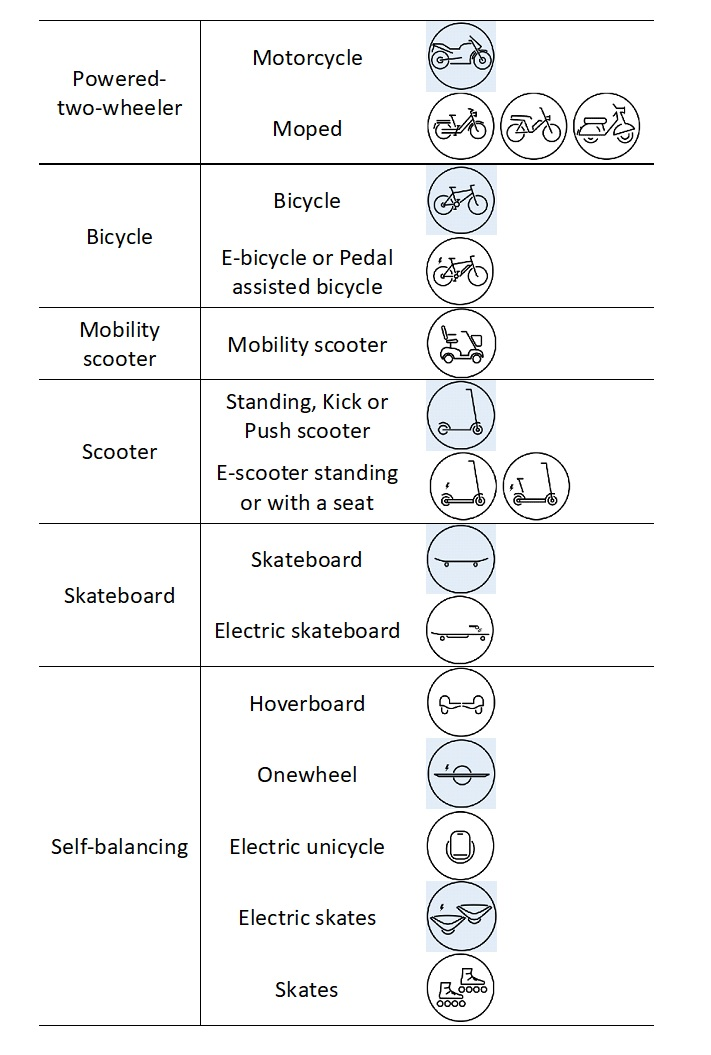
\includegraphics[width=0.5\linewidth]{image/micromobility} \caption{Micromobility (adapted from OECD/ITF (2020)).}\label{fig:unnamed-chunk-23}
\end{figure}

Definitions, classifications and regulatory frameworks for micromobility vary around the world. Bicycles are the smallest vehicle in most countries' classifications. Consequently, a number of micro-vehicles - such as standing e-scooters, e-skateboards and self-balancing vehicles - are excluded from classifications. In some cases, they are classified as toys and are therefore not allowed on public roads. As a temporary solution, Korea has classified these devices as cars. The authorities in Singapore decided to create a new vehicle category called ``Personal Mobility Device'' (PMD). Given the obvious international importance of micro-vehicles and the difficulty in defining and categorising them, it might be useful to develop an internationally recognised classification system for them (OECD/ITF, 2020).

In the \href{https://unece.org/resolutions}{European Union Regulation No.~168/2013}, micromobility vehicles are in class L (UNECE, 2017). Class L vehicles are motorised two-, three- and four-wheeled vehicles. The category uses power, energy source, speed, length, width and height as classification criteria. However, only ``powered electric bicycles with a maximum speed of 25 km/h and a net power of between 250 watts and 1 000 watts'' and ``any two-wheeled vehicle with a maximum design speed of more than 25 km/h and up to 45 km/h and a net power of up to 4 000 watts'' can be classified in the L1e category of ``light two-wheeled motor vehicles''. Other micro-vehicles do not fit into any category. OECD/ITF (2020) proposes to classify micromobility as follows:

\begin{figure}
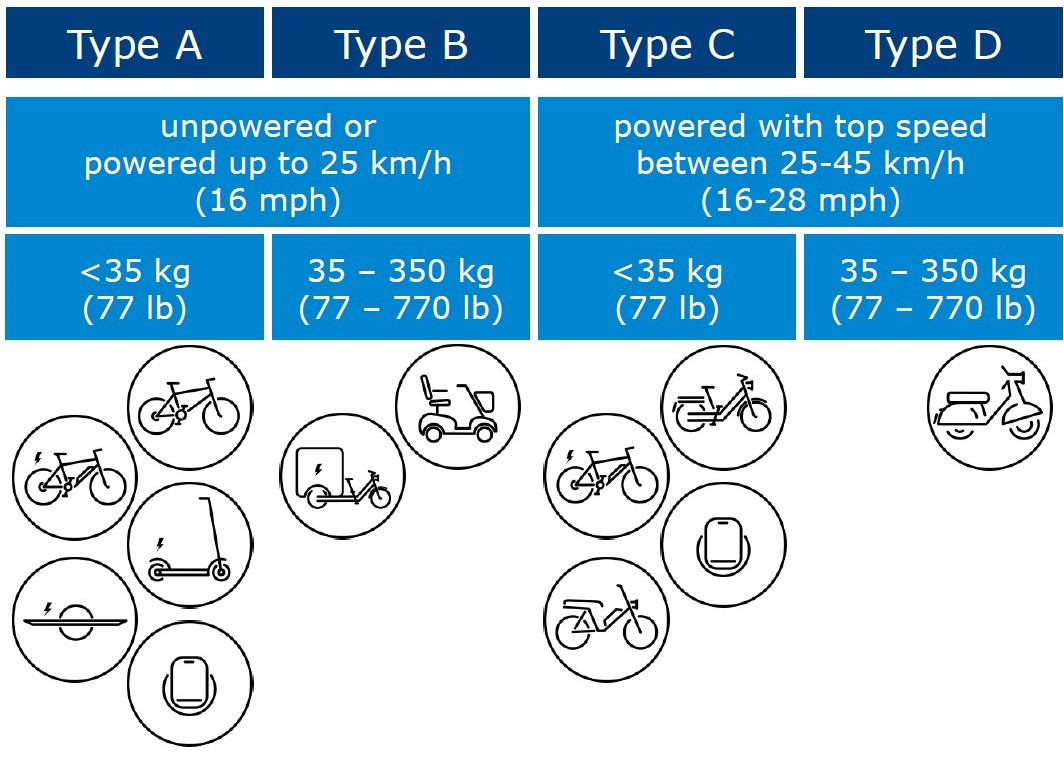
\includegraphics[width=0.5\linewidth]{image/micromobility_classes} \caption{Proposed classification of micro-mobility devices (OECD/ITF (2020).}\label{fig:unnamed-chunk-24}
\end{figure}

In terms of freight transport, \protect\hyperlink{intermodal_freight}{intermodal freight} transport is crucial as a feeder to cities to reduce emissions. In the city centre (see \protect\hyperlink{urban_delivery}{urban deliveries}) there are two main areas that could provide practical and relevant solutions to address the challenges and efficiency of last mile freight transport: (1) freight demand management (FDM) measures and (2) improving parking and charging infrastructure. One FDM measure would be to push for out-of-hours deliveries in order to change the delivery activities of freight forwarders and shippers. Furthermore, receiver prices as well as incentives could play an important role in reducing freight transport. (Holguín-Veras \& Sánchez-Díaz, 2016). In European cities (especially in France), a significant proportion of double-parked delivery vehicles (delivery vehicles parked on the street parallel to parked cars) is observed (Patier et al., 2014). In this context, \protect\hyperlink{space_book}{Smart delivery space booking} could reduce the effects. \protect\hyperlink{passenger_drones}{Passenger drones} and \protect\hyperlink{electric_delivery_fleets}{Electric vehicle delivery fleets} could also reduce some of the externalities of freight transport in cities, but they might also create some new negative externalities.

\hypertarget{key-stakeholders-22}{%
\subsection*{Key stakeholders}\label{key-stakeholders-22}}
\addcontentsline{toc}{subsection}{Key stakeholders}

\begin{itemize}
\tightlist
\item
  \textbf{Affected}: All citizens
\item
  \textbf{Responsible}: Transport service providers and public transport operators, MaaS operators and integrators, city councils, local, regional and national authorities
\end{itemize}

\hypertarget{current-state-of-art-in-research-22}{%
\subsection*{Current state of art in research}\label{current-state-of-art-in-research-22}}
\addcontentsline{toc}{subsection}{Current state of art in research}

EEA (2019) concludes that better F/L/O-mile connectivity in cities can significantly improve environmental and health outcomes. Similar outcome was found in a literature review by Abduljabbar et al.~(2021) for micro-mobility solutions, which showed that micro-mobility solutions help to address a number of transportations challenges like alleviating congestion, addressing inequality and reducing emission. However, realising this potential requires a deep understanding of the different options, their strengths and weaknesses and their impacts on the mobility system as a whole. This is not always easy, as the environmental and health impacts of F/L/O mileage options depend on how they are used and what they replace. This highlights the fact that the increasing availability of e-scooters and digital ride-sharing platforms is changing mobility behaviour in cities, but does not always favour the more climate-friendly choice. A simple example would be a short trip with an e-scooter. If this trip replaces a motorbike or car ride, the environmental and health effects are positive. If it replaces a trip on foot or by bicycle, the situation worsens. More transport options can also lead to people making additional or longer trips, which in turn could worsen the situation. Furthermore, public transport will remain an essential part of any sustainable urban transport system. Good F/L/O-mile options can make public transport more attractive and increase its use, but not replace it completely (EEA, 2019). Laa \& Leth (2020) also notes that e-scooter trips mostly replace trips that would otherwise have been made by a more sustainable mode of transport.

In terms of Environmental sustainability Severengiz et al.~(2020) compares the g CO\textsubscript{2} eq/passenger km (pkm) of different modes of transport (Figure 7.3). Whereby Moreau et al.~(2020) compared shared and private e-scooter and calculated 131g CO\textsubscript{2} eq/pkm for the shared vehicle and 67g CO\textsubscript{2} eq/pkm for the private vehicle.

\begin{figure}
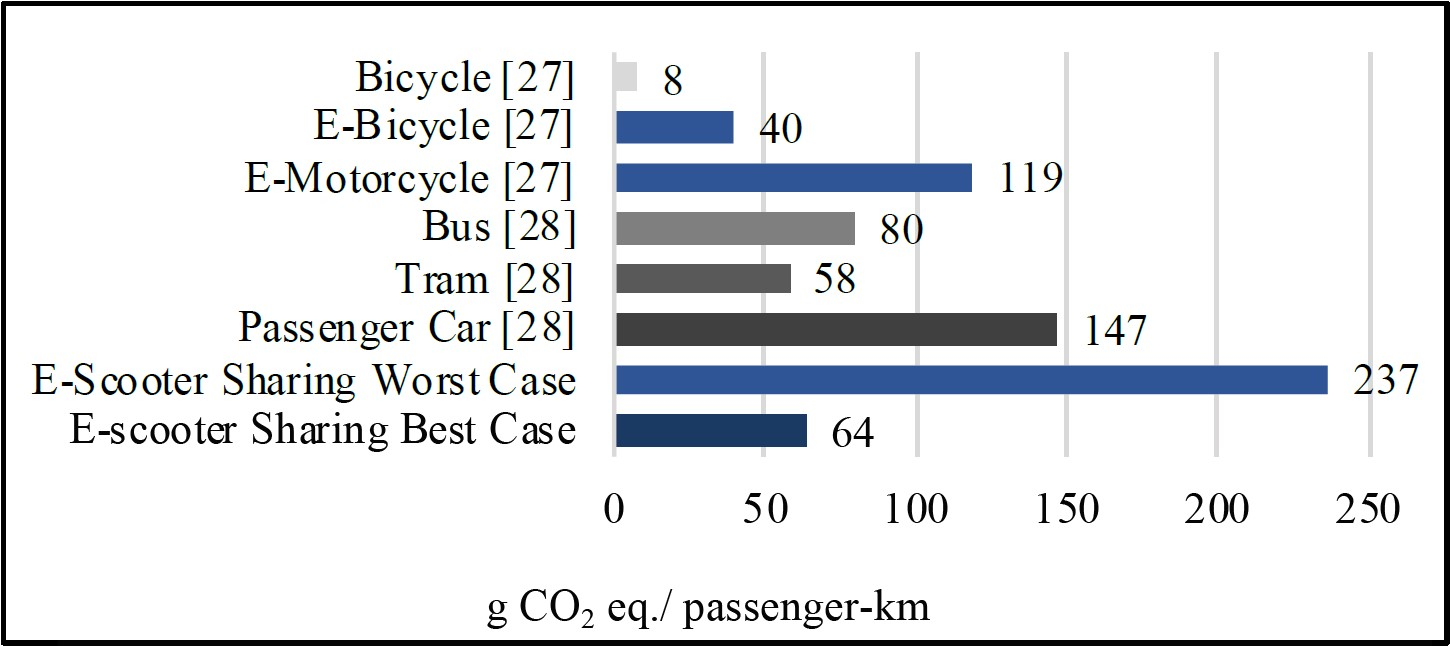
\includegraphics[width=0.5\linewidth]{image/flms_emissions} \caption{Comparison of the CO~2~  equivalent emissions per passenger-km of different modes of transport (Severengiz et al., 2020)}\label{fig:unnamed-chunk-25}
\end{figure}

Accessibility is an indicator of the ability to reach frequently visited places efficiently. This is gaining increasing attention as a complement to the more traditional mobility-based performance measures in transport planning, such as `average delays' and `level of service'. Assessing performance from an accessibility perspective provides a balanced, more holistic approach to transport analysis and planning. In particular, it considers alternative strategies to reduce congestion and mitigate environmental problems, such as promoting efficient, resource-efficient land use policies. Accessibility is a product of mobility and proximity, improved either by increasing the speed of getting between point A and point B (mobility), or by bringing points A and B closer together (proximity), or by a combination of these. In this sense, an accessibility-based approach lends legitimacy to land use initiatives and urban management tools (Cervero, 2005).
However, accessibility is defined differently in the literature. Shin et al.~(2007) measured accessibility using proximity indices (distance and walking time to the nearest metro station). Martínez \& Viegas (2009) defined accessibility by proximity to public transport nodes and the road network. In gravity-like measures, the accessibility of a zone is determined by the destinations that can be reached from that zone, negatively weighted by the travel time, distance or cost between these two zones (Grengs et al., 2010). In the isochronous approach, accessibility is measured as the number of destinations that can be reached within a given travel time (Cervero, 2005). Fan et al., 2012) examined the impact of introducing light rail on transport equity using the cumulative 30-minute accessibility of jobs by public transport. The first and last mile is an important component of a transit trip and determines whether the transit service is accessible or not. Cycling (or other FLM options) reduce transport inequality by increasing the catchment area of public transport so that people can reach more jobs by public transport (Zuo et al., 2020).

However, accessibility is defined differently in the literature. Shin et al.~(2007) measured accessibility using proximity indices (distance and walking time to the nearest metro station). Martínez \& Viegas (2009) defined accessibility by proximity to public transport nodes and the road network. In gravity-like measures, the accessibility of a zone is determined by the destinations that can be reached from that zone, negatively weighted by the travel time, distance or cost between these two zones (Grengs et al., 2010). In the isochronous approach, accessibility is measured as the number of destinations that can be reached within a given travel time (Cervero, 2005). Fan et al.~(2012) examined the impact of introducing light rail on transport equity using the cumulative 30-minute accessibility of jobs by public transport. The first and last mile is an important component of a transit trip and determines whether the transit service is accessible or not. Cycling (or other FLM options) reduce transport inequality by increasing the catchment area of public transport so that people can reach more jobs by public transport (Zuo et al., 2020).

EEA (2019) summarises the lessons learned for systemic change through the use of First/Last/L only mileage options as follows:

\begin{itemize}
\tightlist
\item
  Make the impacts of mobility choices clear and offer alternatives

  \begin{itemize}
  \tightlist
  \item
    Confront road users with the costs incurred by their mobility choices (internalise the external costs of each mode of transport)
  \item
    Offer sufficient and convenient alternatives
  \end{itemize}
\item
  Promote active transport as the first/last/only option for the mile
\item
  Align technology with sustainable mobility goals
\end{itemize}

Bruzzone et al.~(2021) and Nocera et al.~(2020) explore the combination of passenger and freight flows with a focus on the last mile. Such a model is an integrated system in which passengers and goods share vehicles, infrastructure, urban space or more than one of these simultaneously. For example, Fatnassi et al.~(2015) show the potential sustainability gains of sharing goods and passengers in a network with a focus on improving service time and energy waste.

In terms of safety \href{https://www.itf-oecd.org/safe-micromobility}{OECD/ITF} 2020 find out that a trip by car or motorbike in a dense urban area is much more likely to cause fatalities of road users than a trip by a type A micro vehicle. A modal shift from motor vehicles to Type A micro-vehicles can, therefore, make a city safer. A shift from pedestrians to Type A micro-vehicles would have the opposite effect. The safety of e-scooters is likely to improve over the next few years as the users learn to navigate urban traffic and car drivers and pedestrians get used to the new forms of mobility. Safety will also improve as governments introduce safe cycling infrastructure and targeted safety regulations for micro-vehicles and shared mobility services. There are significant regulatory challenges due to the rapid pace of innovation in micro-vehicle development. They suggest the following measures to improve the safety of micro-mobility:

\begin{itemize}
\tightlist
\item
  Provide protected space for micro-mobility and keep pedestrians safe (Where pedestrians do not feel safe on pavements, the number of people walking will decrease).
\item
  Low speeds of e-scooters and e-bikes should be regulated as bicycles, higher speeds of micro-mobiles as mopeds
\item
  Collect data on micro-vehicle trips and accidents (in order to pro-actively manage the safety performance of road networks)
\item
  Incorporate micro-mobility into road user education
\item
  Combat drunk driving and speeding for all types of vehicles
\item
  Remove incentives for micro-mobile drivers to speed (Minute-by-minute rental can be an incentive to speed or ignore traffic rules. Alternatives include a fixed driving fee, a distance-based fee or a membership fee).
\item
  Improve micro-vehicle design (Micro-vehicle manufacturers should try to improve stability and road grip. Solutions could be found in pneumatic tyres, larger wheels and frame geometry, but also in areas that still need to be explored).
\item
  Reduce general risks associated with micro-mobility sharing (minimise vehicle kilometres driven by escort vehicles for moving or charging micro-mobility devices, use removable or higher capacity batteries and plug-in docks, allocate space for on-street parking of micro-vehicles).
\end{itemize}

Reck et al.~(2022) found that shared e-scooters and e-bikes emit more CO\textsubscript{2} than the transport modes they replace. In contrast, private/personal e-scooters and e-bikes emit less than the transport modes they replace. This finding might be important for planners to test the effectiveness of policy interventions through transport simulations when it comes to micro-mobility and it's variety of vehicle types.

\hypertarget{current-state-of-art-in-practice-22}{%
\subsection*{Current state of art in practice}\label{current-state-of-art-in-practice-22}}
\addcontentsline{toc}{subsection}{Current state of art in practice}

A new coalition, Micro-mobility for Europe (MMfE), has come together in Europe in 2021. Eight e-scooter operators (Bird, Bolt, Dott, FreeNow, Lime, TIER, Voi and Wind) want to contribute to the development of a coherent policy framework in Europe through this coalition (Intelligent Transport, 2021).

Research and Markets (2021) names bike sharing, kick scooter sharing and scooter sharing as the dominant micro-mobility sharing modes. By 2020, the global fleet was around 20.5 million vehicles and the market value was at \$44.12 billion while it is projected to reach \$214.57 by 2030 (Yadav et al, 2022). Globally, bike sharing is currently estimated to account for almost 98\% of the fleet size of the micro-mobility market. The most important factor cited is the advancement of technologies. Innovations mentioned are infrastructure solutions (e.g.~smart docking stations, solar-powered charging stations and mobility hubs), hardware solutions (e.g.~smart locks and sensors) and high-end software solutions (e.g.~mapping and navigation, fleet security, real-time fleet data and analytics, and smart fleet management), driven by AI engines and IoT sensors. Micro-mobility business models such as public-private partnerships, private bike-sharing schemes and non-profit programmes are evolving and micro-mobility systems continue to be embedded in municipal transport and become an integral part of the emerging Mobility-as-a-Service (MaaS) ecosystem.

In 2018, the first full year after the launch of e-scooter sharing, Americans have already taken 38.5 million trips on shared e-scooters (compared to station-based bike sharing with 36.5 million trips, which has been on the market for almost ten years). Electrically powered micro-mobility is projected as the most lucrative in the propulsion type segment, while bicycles are the most profitable when it comes to vehicle types. However, existing demand for other micro-mobility are not predicted to decrease (Yadav et al., 2022). Which indicates that it makes sense to support different models/vehicles. Considering the high demand and rapid adoption of micro-mobility options, the expected global market potential is over \$500 billion by 2030 (Eliasen, 2021). In comparison, the micro-mobility market in Europe is estimated to be worth over 100 billion euros in 2030 (Twisse, 2020).
Most new micro-mobility platform start-ups (mainly e-scooters) were initially unprofitable because the operational costs of running e-scooters (charging, repair/maintenance, insurance and payment fees) were so high that the payback period for the initial scooter purchase was shorter than the lifetime of the scooter, resulting in a negative return on investment per scooter. According to Travis VanderZanden, CEO of Bird, the profitability of the units has improved significantly in recent years due to improvements in the durability of the scooters and price increases for customers (Eliasen, 2021). Reck et al.~(2021) looked at the use of shared micro-mobility in Zurich and found that the adoption rate of e-scooters is the highest (28\%), compared to docked (e-) bikes (16\%) and dockless (e-) bikes (9\%), although e-scooter ownership is uncommon (3\%) compared to e-bike ownership (14\%). Additionally they found, that micro-mobility users tend to be young, well-educated, affluent males and shared e-scooter users are the most representative of the larger population.

Haas (2018) identifies four challenges that need to be addressed to make FLM attractive:

\textbf{Challenge 1: Accessibility}
It happens quite often that no sharing transport can be offered in the vicinity. \emph{``On average, our customers are willing to walk 300 metres to a car.''} says Olivier Reppert, (head of the car-sharing market leader Car2go). \emph{``If that doesn't work several times, they jump off.''} The company is, therefore , working hard to bring the vehicles as close as possible to the customers. \emph{``We know very precisely where which car should be at which time.''} says Reppert. This can be determined precisely through anonymous data collection. But: \emph{``Today, we are not yet in a position to always target exactly these points.''} Reppert has high expectations for the future use of autonomous vehicles that move themselves to carsharing hotspots: \emph{``Then we would only need 50 per cent of the current fleet to serve the same demand.''} he says.

\textbf{Challenge two: The combination}
To enable the perfect combination of the different offers, an app is needed that includes all options and coordinates them with each other. So far, there are only a few such apps with as many means of transport as possible in the cities. This could improve if the cities, which should have the best overview of the available means in their area, take the lead themselves.

\textbf{Challenge three: The legal situation}
\emph{``If various small vehicles simply share the footpaths, cycle paths or roads, this will lead to more accidents''} says Markus Friedrich (professor of traffic planning and traffic control technology at the University of Stuttgart). However, there is not enough space to offer a separate lane for each type. He, therefore, sees the solution in a change to the current speed limits in the road traffic regulations: \emph{``With a standard speed of 30km/h, vehicles can share the road space better.''} says the professor. \emph{``And as soon as many vehicles have electric drives, a limit of 20km/h is conceivable in the current 30km/h speed zones.''} On main urban roads, higher speeds could still be allowed.

\textbf{Challenge four: The public transport upgrade}
The numerous additional services could not only complement but replace bus and rail. Demand could increase significantly if the advantages of the gained efficiency unfold - from higher availability to cheaper prices. Therefore, public transport must be made faster so that it offers a travel time advantage. What is needed, Friedrich says, are express buses and express trains that are given their own routes and do not stop as often as before. Many cities would need a much denser frequency or additional express trains.

\hypertarget{relevant-initiatives-in-austria-22}{%
\subsection*{Relevant initiatives in Austria}\label{relevant-initiatives-in-austria-22}}
\addcontentsline{toc}{subsection}{Relevant initiatives in Austria}

\textbf{Passenger FLM}

\begin{itemize}
\tightlist
\item
  E-scooters

  \begin{itemize}
  \tightlist
  \item
    \href{https://autorevue.at/ratgeber/e-scooter-wien-vergleich}{Autorevue.at}
  \item
    \href{https://www.stadt-wien.at/wien/news/e-scooter-sharing-system-in-wien.html}{Stadt-wien.at}
  \item
    \href{https://www.wien.gv.at/verkehr/scooter-roller/index.html}{Wien.gv.at}
  \item
    \href{https://www.oeamtc.at/thema/fahrrad/e-kleintretroller-e-scooter-in-oesterreich-31721872}{Öamtc.at}
  \item
    \href{https://www.oesterreich.gv.at/themen/freizeit_und_strassenverkehr/Elektro-Scooter,-Quads-und-Co/Seite.610110.html}{Österreich.gv.at}
  \end{itemize}
\item
  Bicycle and E-Bicycle hire

  \begin{itemize}
  \tightlist
  \item
    \href{https://firmenradl.at/cms/}{Firmenradl.at}
  \item
    \href{https://www.citybikewien.at/de}{Citybikewien}
  \item
    \href{http://www.citybikesalzburg.at/}{Citybikesalzburg}
  \item
    \href{https://www.nextbike.at/de/niederoesterreich/}{Nextbike}
  \item
    \href{https://www.tips.at/nachrichten/linz/land-leute/523512-linzer-radverleih-startet-im-fruehjahr-an-40-standorten}{Tpis.at}
  \end{itemize}
\item
  Car sharing

  \begin{itemize}
  \tightlist
  \item
    \href{https://www.vcoe.at/presse/presseaussendungen/detail/carsharing-haushalte-potential-2018}{VCÖ}
  \item
    \href{https://www.carsharing-wien.com/anbieter/oebb-rail-and-drive}{ÖBB}
  \end{itemize}
\item
  Ride-hailing \& Ride-sharing

  \begin{itemize}
  \tightlist
  \item
    \href{https://www.ots.at/presseaussendung/OTS_20210113_OTS0026/free-now-will-als-erste-mobilitaetsplattform-in-europa-bis-2030-null-emissionen-erreichen}{Ots.at}
  \item
    \href{https://www.umweltberatung.at/carsharing-mitfahrboersen}{Umweltberatung.at}
  \item
    \href{https://greendrive.at/premium/\#benefits}{Greendrive.at}
  \item
    \href{https://www.carployee.com/\#start-section}{Carployee.com}
  \item
    \href{https://ummadum.com/}{Ummadum.com}
  \end{itemize}
\item
  Mobility-as-a-Service

  \begin{itemize}
  \tightlist
  \item
    \href{https://www.austriatech.at/assets/Uploads/Publikationen/PDF-Dateien/29fc02ada2/MaaS-miA_english_102019_web.pdf}{AustriaTech.at}
  \item
    \href{https://maas-ready.at}{maas-ready.at}
  \item
    \href{https://www.ultimob.at}{ultimob.at}
  \item
    \href{https://www.tim-oesterreich.at/graz/}{tim-oesterreich.at}
  \item
    \href{https://wegfinder.at/}{wegfinder.at}
  \item
    \href{https://www.wienerlinien.at/eportal3/ep/channelView.do/pageTypeId/66526/channelId/-3600060}{wienerlinien.at}
  \item
    \href{https://anachb.vor.at/}{anachb.vor.at}
  \end{itemize}
\item
  Passenger drones

  \begin{itemize}
  \tightlist
  \item
    \href{https://brutkasten.com/autonome-lufttaxis-linz-ag-facc-ehang/}{Derbrutkasten.com}
  \item
    \href{https://www.derstandard.at/consent/tcf/story/2000103120464/erste-teststrecke-fuer-e-lufttaxis-2020-in-linz}{Derstandard.at-1}
  \item
    \href{https://www.derstandard.at/consent/tcf/story/2000122402408/flugtaxis-wann-kommt-der-tesla-der-luefte}{Derstandard.at-2}
  \end{itemize}
\item
  Demand responsive transit

  \begin{itemize}
  \tightlist
  \item
    \href{https://www.bedarfsverkehr.at/content/Literatur}{Bedarfsverkehr.at}
  \item
    \href{https://repositum.tuwien.at/handle/20.500.12708/1312}{Repositum.tuwien.at}
  \item
    \href{https://projekte.ffg.at/projekt/2929323}{Projekte.ffg.at}
  \end{itemize}
\item
  Mobility hubs

  \begin{itemize}
  \tightlist
  \item
    \href{https://www.wienerlinien.at/web/wiener-linien/wienmobil-stationen}{Wienmobil-stationen}
  \item
    \href{https://www.tim-oesterreich.at/}{Tim-oesterreich}
  \item
    \href{https://www.wien.gv.at/stadtentwicklung/studien/pdf/b008521.pdf}{Wien.gv.at}
  \end{itemize}
\end{itemize}

\textbf{Freight FLM}

\begin{itemize}
\tightlist
\item
  Urban Deliveries

  \begin{itemize}
  \tightlist
  \item
    \href{https://www.logistik2030.at/?page_id=268}{Logistik2030.at-1}
  \item
    \href{https://infothek.bmk.gv.at/gruene-stadtlogistik-post-testet-city-hubs-in-wien/}{Infothek.bmk.gv.at}
  \item
    \href{https://www.logistik2030.at/?page_id=63}{Logistik2030.at-2}
  \item
    \href{https://www.remihub.at/}{Remihub.at}
  \item
    \href{https://logpoint.at/ueber-uns/gruene-logistikwelt-und-standorte/}{Logpoint.at}
  \item
    \href{https://www.wu.ac.at/scm/projekte/}{Wu.ac.at}
  \item
    \href{https://www.post.at/p/c/vorzimmer-zustellung}{Post.at}
  \end{itemize}
\item
  Smart delivery space booking

  \begin{itemize}
  \tightlist
  \item
    \href{https://www.ots.at/presseaussendung/OTS_20150123_OTS0044/simple-stressfreie-ladezonensuche-wk-wien-praesentiert-neue-app}{Ots.at}
  \item
    \href{https://www.wko.at/service/verkehr-betriebsstandort/Ladezonen-Nutzung.html}{WKO1}
  \item
    \href{https://www.wko.at/service/w/verkehr-betriebsstandort/ladezone-wien-app.html}{WKO2}
  \item
    \href{https://www2.ffg.at/verkehr/projekte.php?id=805\&lang=de\&browse=programm}{FFG}
  \end{itemize}
\item
  Delivery drones

  \begin{itemize}
  \tightlist
  \item
    \href{https://www.oeamtc.at/thema/drohnen/drohnen-info-app-26853120}{Öamtc.at}
  \end{itemize}
\item
  Freight hubs

  \begin{itemize}
  \tightlist
  \item
    \href{https://infrastruktur.oebb.at/en/partners/terminals/locations/terminal-wien-sued}{Infrastruktur.oebb.at}
  \item
    \href{https://dhl-freight-connections.com/de/unternehmen/dhl-eroffnet-hochmodernes-logistikdrehkreuz-am-flughafen-wien/}{DHL-freight-connections.com}
  \item
    \href{https://www.logistik2030.at/?page_id=63}{Logistik2030.at}
  \item
    \href{https://www.thinkportvienna.at/ueber-uns/projekte/}{Thinkportvienna.at}
  \item
    \href{https://www.hafen-wien.com/de/home}{Hafen-wien.com}
  \end{itemize}
\end{itemize}

See also \protect\hyperlink{shared}{shared mobility section}.

\hypertarget{impacts-with-respect-to-sustainable-development-goals-sdgs-22}{%
\subsection*{Impacts with respect to Sustainable Development Goals (SDGs)}\label{impacts-with-respect-to-sustainable-development-goals-sdgs-22}}
\addcontentsline{toc}{subsection}{Impacts with respect to Sustainable Development Goals (SDGs)}

\begin{longtable}[]{@{}
  >{\centering\arraybackslash}p{(\columnwidth - 8\tabcolsep) * \real{0.2029}}
  >{\centering\arraybackslash}p{(\columnwidth - 8\tabcolsep) * \real{0.1884}}
  >{\centering\arraybackslash}p{(\columnwidth - 8\tabcolsep) * \real{0.2029}}
  >{\centering\arraybackslash}p{(\columnwidth - 8\tabcolsep) * \real{0.2029}}
  >{\centering\arraybackslash}p{(\columnwidth - 8\tabcolsep) * \real{0.2029}}@{}}
\toprule()
\begin{minipage}[b]{\linewidth}\centering
Impact level
\end{minipage} & \begin{minipage}[b]{\linewidth}\centering
Indicator
\end{minipage} & \begin{minipage}[b]{\linewidth}\centering
Impact direction
\end{minipage} & \begin{minipage}[b]{\linewidth}\centering
Goal description and number
\end{minipage} & \begin{minipage}[b]{\linewidth}\centering
Source
\end{minipage} \\
\midrule()
\endhead
Systemic & Reduction in transit service inequality & \textbf{+} & Equality (\emph{5,10}) & Zuo et al., 2020a \\
Systemic & Reduction in negative externalities but substitution of more environmentally friendly modes e.g.~walking & \textbf{\textasciitilde{}} & Environmental sustainability (\emph{7,12,13,15}) & Twisse, 2020 \\
Systemic & Profits from growth in micromobility sector (F/L/O options) & \textbf{+} & Sustainable economic development (\emph{8,11}) & Goessling, 2020 \\
Systemic & Improvement in technology of micro-mobility equipment & \textbf{+} & Innovation \& Infrastructure (\emph{9}) & Eliasen, 2021 \\
\bottomrule()
\end{longtable}

\hypertarget{technology-and-societal-readiness-level-22}{%
\subsection*{Technology and societal readiness level}\label{technology-and-societal-readiness-level-22}}
\addcontentsline{toc}{subsection}{Technology and societal readiness level}

\begin{longtable}[]{@{}cc@{}}
\toprule()
TRL & SRL \\
\midrule()
\endhead
7-9 & 6-7 \\
\bottomrule()
\end{longtable}

\hypertarget{further-links-18}{%
\subsection*{Further links}\label{further-links-18}}
\addcontentsline{toc}{subsection}{Further links}

\begin{itemize}
\tightlist
\item
  \href{https://unece.org/resolutions}{UNECE.org}
\item
  \href{https://www.eltis.org/resources/case-studies/rise-micromobility}{ELTIS.org}
\end{itemize}

\hypertarget{references-22}{%
\subsection*{References}\label{references-22}}
\addcontentsline{toc}{subsection}{References}

\begin{itemize}
\tightlist
\item
  Abduljabbar, R. L., Liyanage, S., Dia, H. (2021). The role of mirco-mobility in shaping sustainable cities: A systematic literature review. Transportation Research Part D. 92, 102734. \url{https://doi.org/10.1016/j.trd.2021.102734}
\item
  Arvidsson, N., Givoni, M., \& Woxenius, J. (2016). Exploring last mile synergies in passenger and freight transport. Built Environment, 42(4), 523--538. \url{https://doi.org/10.2148/benv.42.4.523}
\item
  Bruzzone, F., Cavallaro, F., \& Nocera, S. (2021). The integration of passenger and freight transport for first-last mile operations. Transport Policy, 100, 31--48. \url{https://doi.org/10.1016/j.tranpol.2020.10.009}
\item
  Cervero, R. (2005). Accessible Cities and Regions: A Framework for Sustainable Transport and Urbanism in the 21st Century. \url{https://doi.org/10.11436/mssj.15.250}
\item
  City database \textbar{} Eltis. (2021, July 19). \url{https://www.eltis.org/mobility-plans/city-database}
\item
  EEA, E. E. A. (2019). The first and last mile --- the key to sustainable urban transport (Issue 18).
\item
  Eliasen, J. (2021, January 15). The Future of Micromobility. How VCs and E-Scooters kicked off the\ldots{} \textbar{} by Jason Eliasen \textbar{} The Startup \textbar{} Medium. \url{https://medium.com/swlh/the-future-of-micromobility-2d4d96d4e2dd}
\item
  Fan, Y., Guthrie, A., \& Levinson, D. (2012). Impact of light-rail implementation on labor market accessibility. Journal of Transport and Land Use, 5(3), 28--39.
\item
  Fatnassi, E., Chaouachi, J., \& Klibi, W. (2015). Planning and operating a shared goods and passengers on-demand rapid transit system for sustainable city-logistics. Transportation Research Part B: Methodological, 81, 440--460. \url{https://doi.org/10.1016/j.trb.2015.07.016}
\item
  Furth, P. G., Mekuria, M. C., \& Nixon, H. (2016). Network Connectivity for Low-Stress Bicycling. Transportation Research Record, 2587(1), 41--49. \url{https://doi.org/10.3141/2587-06}
\item
  Gössling, S. (2020). Integrating e-scooters in urban transportation: Problems, policies, and the prospect of system change. Transportation Research Part D: Transport and Environment, 79(January), 102230. \url{https://doi.org/10.1016/j.trd.2020.102230}
\item
  Grengs, J., Levine, J., Shen, Q., \& Shen, Q. (2010). Intermetropolitan Comparison of Transportation Accessibility: Sorting Out Mobility and Proximity in San Francisco and Washington, D.C. Journal of Planning Education and Research, 29(4), 427--443. \url{https://doi.org/10.1177/0739456X10363278}
\item
  Haas, C. (2018, November 13). Nahverkehr: So lässt sich die letzte Meile nach Hause bequem zurücklegen - WELT. \url{https://www.welt.de/wirtschaft/article183688842/Nahverkehr-So-laesst-sich-die-letzte-Meile-nach-Hause-bequem-zuruecklegen.html}
\item
  Holguín-Veras, J., \& Sánchez-Díaz, I. (2016). Freight Demand Management and the Potential of Receiver-Led Consolidation programs. Transportation Research Part A: Policy and Practice, 84, 109--130. \url{https://doi.org/10.1016/j.tra.2015.06.013}
\item
  Intelligent Transport. (2021, February 2). Big names across micromobility sector form European coalition. \url{https://www.intelligenttransport.com/transport-news/116405/micromobility-for-europe/}
\item
  Laa, B., \& Leth, U. (2020). Survey of E-scooter users in Vienna: Who they are and how they ride. Journal of Transport Geography, 89(October), 102874. \url{https://doi.org/10.1016/j.jtrangeo.2020.102874}
\item
  Martínez, L. M., \& Viegas, J. M. (2009). Effects of Transportation Accessibility on Residential Property Values: Hedonic Price Model in the Lisbon, Portugal, Metropolitan Area. Transportation Research Record, 2115(1), 127--137. \url{https://doi.org/10.3141/2115-16}
\item
  Moreau, H., de Meux, L. J., Zeller, V., D'Ans, P., Ruwet, C., \& Achten, W. M. J. (2020). Dockless e-scooter: A green solution for mobility? Comparative case study between dockless e-scooters, displaced transport, and personal e-scooters. Sustainability (Switzerland), 12(5). \url{https://doi.org/10.3390/su12051803}
\item
  Nocera, S., Pungillo, G., \& Bruzzone, F. (2020). How to evaluate and plan the freight-passengers first-last mile. Transport Policy. \url{https://doi.org/10.1016/j.tranpol.2020.01.007}
\item
  OECD/ITF. (2020). Safe Micromobility. 98.
\item
  Oeschger, G., Carroll, P., \& Caulfield, B. (2020). Micromobility and public transport integration: The current state of knowledge. Transportation Research Part D: Transport and Environment, 89, 102628. \url{https://doi.org/10.1016/j.trd.2020.102628}
\item
  Patier, D., David, B., Chalon, R., \& Deslandres, V. (2014). A New Concept for Urban Logistics Delivery Area Booking. Procedia - Social and Behavioral Sciences, 125, 99--110. \url{https://doi.org/10.1016/j.sbspro.2014.01.1459}
\item
  Reck, D. J., Axhausen, K.W. (2021). Who uses shared micro-mobility services? Empirical evidence from Zurich, Switzerland. Transportation Research Part D: Transportation and Environment. 94, 102803. \url{https://doi.org/10.1016/j.trd.2021.102803}
\item
  Reck, D. J., Martin, H., Ayhausen, K. W. (2022). Mode choice, substitution patterns and environmental impacts of shared and personal micro-mobility. Transportation Research Part D. 102, 103134.
\item
  Research and Markets. (2021, June 15). Global Micromobility (Bikes, Scooters, Kick-scooters) Markets Report 2021-2025 - Future Growth Potential Enhanced by Opportunities Due to Government Push, Regulatory Reforms and Advancement in Technologies. \url{https://www.prnewswire.com/news-releases/global-micromobility-bikes-scooters-kick-scooters-markets-report-2021-2025---future-growth-potential-enhanced-by-opportunities-due-to-government-push-regulatory-reforms-and-advancement-in-technologies-301312406.html}
\item
  Severengiz, S., Finke, S., Schelte, N., \& Wendt, N. (2020). Life Cycle Assessment on the Mobility Service E-Scooter Sharing. 2020 IEEE European Technology and Engineering Management Summit, E-TEMS 2020, September. \url{https://doi.org/10.1109/E-TEMS46250.2020.9111817}
\item
  Shin, K., Washington, S., \& Choi, K. (2007). Effects of Transportation Accessibility on Residential Property Values: Application of Spatial Hedonic Price Model in Seoul, South Korea, Metropolitan Area. Transportation Research Record, 1994(1), 66--73. \url{https://doi.org/10.3141/1994-09}
\item
  Twisse, F. (2020, August 12). The rise of micromobility \textbar{} Eltis. \url{https://www.eltis.org/resources/case-studies/rise-micromobility}
\item
  UNECE. (2017). ECE R78 - Consolidated Resolution on the Construction of Vehicles. United Nations Economic and Social Council, July. Available at: \url{https://unece.org/resolutions} (Accessed: 22/07/2021)
\item
  Winters, M., Davidson, G., Kao, D., \& Teschke, K. (2011). Motivators and deterrents of bicycling: Comparing influences on decisions to ride. Transportation, 38(1), 153--168. \url{https://doi.org/10.1007/s11116-010-9284-y}
\item
  Yadav, P., Mutreja, S. (2022). Micromobility Market by Propulsion Type, Vehicle Type, Sharing Type and Age Group: Global Opportunity Analysis and Industry Forecast, 2021-2030. Available at: \url{https://www.alliedmarketresearch.com/micro-mobility-market-A11372} {[}Accessed: 09th of July 2022{]}
\item
  Zuo, T., Wei, H., Chen, N., \& Zhang, C. (2020a). First-and-last mile solution via bicycling to improving transit accessibility and advancing transportation equity. Cities, 99, 102614. \url{https://doi.org/10.1016/j.cities.2020.102614}
\item
  Zuo, T., Wei, H., \& Rohne, A. (2018). Determining transit service coverage by non-motorized accessibility to transit: Case study of applying GPS data in Cincinnati metropolitan area. Journal of Transport Geography, 67, 1--11. \url{https://doi.org/10.1016/j.jtrangeo.2018.01.002}
\end{itemize}

\hypertarget{dist_time_fares}{%
\section{Transit fares}\label{dist_time_fares}}

\textbf{Updated: 13th July 2022}

\hypertarget{definition-23}{%
\subsection*{Definition}\label{definition-23}}
\addcontentsline{toc}{subsection}{Definition}

Fares are fundamental element of transit operations, they have an important impact on ridership dynamics and the financial vitality of transit agencies (El-Geneidy et al., 2016; Zhao \& Zhang, 2019). The way fares are set and subsequently adjusted is inherently complex. On the one hand, there is an attempt to ensure equity for the population and, on the other hand, to generate sufficient revenue for the transit agency (Brown, 2018; Yoh et al., 2016). In current transportation research, fares and especially fare structures (such as zone-based or distance-based fares) are argued to have negative effects on equity, although there is also evidence that it depends on where one lives and how this affects the degree of accessibility (Martens, 2012).

There is no universally accepted definition of equity in the context of public transport, but different ways of measuring equity from different perspectives, such as travel distance, time, comfort, and monetary costs. A necessary condition for the scientific measurement of equity in public transport is to focus on a specific dimension, such as monetary costs (fares) (Wang et al., 2021).

Three defining dimensions for assessing fairness can be identified in the literature on distributive justice (Rubensson et al., 2020):

\begin{itemize}
\tightlist
\item
  A normative dimension - the foundations of the fairness principle: e.g., should all outcomes be as similar as possible, or should all the people have as similar opportunities as possible, or should well-regulated markets be trusted to produce the fairest outcome?
\item
  Authors choose what to measure - equity of inputs (fares, taxes), outputs (accessibility, geographic coverage), or consumption (trips made) of public transportation.
\item
  Distributional differences - assessing horizontal equity (equity among members of the same group, such as all public transport users or all citizens) or vertical equity (equity among members of different groups, such as different income, age, or occupational groups).
\end{itemize}

A fare system typically contains four basic components (Streeting \& Charles, 2006):

\begin{itemize}
\tightlist
\item
  Fare media - Paper tickets or smart cards
\item
  Fare product - Range of available ticket types, such as frequency-based discounts and off-peak discounts, fare limitation to a fixed maximum amount on weekends (Chalabianlou et al., 2015; Guzman et al., 2014)
\item
  Fare structure
\item
  Fare level - Fares can be set at a flat rate or differentiated. Differentiation is usually proposed to achieve a fare system that lowers demand for trips with high production costs and increases demand for trips with low production costs, thus increasing revenues on the one hand and lowering prices for some users on the other (Rubensson et al., 2020).
\end{itemize}

The different fare structures are (Wang et al., 2021):

\begin{itemize}
\tightlist
\item
  \textbf{Flat fares} (a single fare for the entire fare system)
\item
  \textbf{Distance-based fares} (fares calculated by distance)
  A distanced-based system charges higher fares for passengers that cover longer distances. The fares are typically calculated on a route-by-route basis where it is based on the distance between origin and destination (OD). Distance-based fares are typically complicated to develop and enforce because they require a card to be swiped, tapped or punched for bus or rail, or they require a barrier that enforces additional payment. Furthermore, distance-based pricing is not frequently used in non-express routes and rail and it is more common for express routes and systems that radiate from a central area (McKone, 2010).
\item
  \textbf{Time-based fares} (fares calculated by travel time)
  The time-based system allows passengers to use public transport and make free transfers in a set period of time. The validity period can be as short as 20 min (Krakow.pl, 2021) or an unlimited weekly, monthly or yearly pass (Wiener Linien, 2021). Importantly, this pricing system requires some sort of card (paper, magnetic or smart card) to issue the transfer. It is often used for within-city public transport solutions.
\item
  \textbf{Zone-based fares} (fares calculated by travel zone)
  The fares are typically calculated based on the zones that establish increasing fares in certain regions of the city (e.g.~in Paris commuter rail system or London Underground) (McKone, 2010).
\end{itemize}

Moreover, Brown (2018) mentions five types of fare structuring: flat, adjusted to distance travelled, variable by time of day, variable by mode, and/or discounted based on rider characteristics.

\hypertarget{key-stakeholders-23}{%
\subsection*{Key stakeholders}\label{key-stakeholders-23}}
\addcontentsline{toc}{subsection}{Key stakeholders}

\begin{itemize}
\tightlist
\item
  \textbf{Affected}: Public Transport Passengers, Public Transport Operators
\item
  \textbf{Responsible}: Local and National Governments, Transport Agencies authorities
\end{itemize}

\hypertarget{current-state-of-art-in-research-23}{%
\subsection*{Current state of art in research}\label{current-state-of-art-in-research-23}}
\addcontentsline{toc}{subsection}{Current state of art in research}

The main issue currently being studied is equity under different fare systems (Brown, 2018; El-Geneidy et al., 2016; Rubensson et al., 2020; Wang et al., 2021; Zhao \& Zhang, 2019).

Rubensson et al.~(2020) find that in terms of horizontal equity (between public transport users and the public in general), distance fares offer the highest level of equality (0.04), followed by zone fares (0.07) and then flat fares (0.1) as measured by the \href{https://www.univie.ac.at/sowi-online/esowi/cp/einfsoz/einfsoz-55.html}{Gini coefficient}. However, in terms of vertical equity (across income groups), travellers from low-income areas pay a larger share of fares than higher-income travellers in all fare systems. They further conclude that as the distance-dependence of fares decreases, vertical equity increases and that an increasing distance-dependent fare system leads to increasing horizontal equity.

Brown (2018) concludes in a study of the effects of pricing on the equity in mass transit in Los Angeles that any type of fare variation improves equity compared to flat fares when the three criteria of equity (benefits received, ability to pay, and cost) are considered. In particular, a fare structure that includes both a per-mile fare and discounts for off-peak trips produces the most equitable results, as low-income passengers travel significantly shorter distances, ride more local buses, and make a smaller share of trips during peak hours. This also better reflects the marginal cost of providing the service. A slightly lower per-mile fare for low-income riders usually does not truly reflect the relative ability of those riders to pay if the fares are not cheap enough (e.g., LA Metro Rider Relief coupons to reduce the cost to riders by 10 percent (Los Angeles County Metropolitan Transportation Authority, 2021)). For example, if low-income riders are to be encouraged, households earning 50 percent of the area-wide median income should receive a 50 percent discount on the per-mile fare. This option is available in San Francisco right now (San Francisco Municipal Transportation Agency, 2021). Brown (2018) concludes that income-based discounts on flat fares would improve equity (as measured by the ability-to-pay criterion), but would likely not always reflect equity as measured by mileage or time-based cost variation. Instead, a distance-based and discounted off-peak fare structure is the best solution for all three equity criteria. Smart card technology has made the introduction and enforcement of variable fares much easier than in the past, and new transportation and financial innovations have made passengers more comfortable with variable fares on mass transit.

Wang et al.~(2021) propose new fare equity evaluation measures using \protect\hyperlink{contactless_cards}{smart card} data. These systems generate large volumes of transaction records from individual passenger trips and contain the information needed to map, measure, and monitor fare equity. In their study they conclude that adopting a more coarsely zoned structure, reducing variation in fare levels, and changing fare incentives will increase ridership, improve revenue, and offset fare disparities and improve fare equity across ridership types and urban area.

In 2022, free public transport is still researched in various aspects. The increase in overall public transport travel is one of the most appealing factors nowadays and is seen in all papers. Highest rates of growth is mostly observed with young and elderly people, while elderly people respond more strongly to discount measures than students. Still, existing literature states, that free-fare discounts are expensive policies with quite low efficiency (Tomes et al., 2022; Bull et al., 2021). Other looked at fare systems involving e-ticketing/smart ticketing to improve customer management, planning and convenience (Hojski et al.~2022) and is also discussed more in the next chapter (\protect\hyperlink{maas}{MaaS}).

\hypertarget{current-state-of-art-in-practice-23}{%
\subsection*{Current state of art in practice}\label{current-state-of-art-in-practice-23}}
\addcontentsline{toc}{subsection}{Current state of art in practice}

According to Brown (2018) flat fares are the most common around the world and prevalent in the U.S., but these do not necessarily lead to equitable outcomes for passengers. Although equity is an important goal for most transit agencies, fare discussions are often influenced by budgetary concerns, rising operating costs, and aversion to public backlash. This creates a paradox between desired goals and current practices.

The prices of public transport for users vary greatly as a statistic of public transport single tickets worldwide shows (Figure 1). Also within a country the prices vary greatly as a report of the ADAC (2019) demonstrates. At 109.20 euros, the monthly ticket in Hamburg is almost twice as expensive as in Munich. However, in Hamburg you can still travel far beyond the city limits. The average monthly ticket in Germany costs 77.50 euros. Day tickets cost an average of 7.02 euros. In some cities it is valid for 24 hours from the time of validation and in others it is only valid for the day of validation, but often until well after midnight.

\begin{figure}
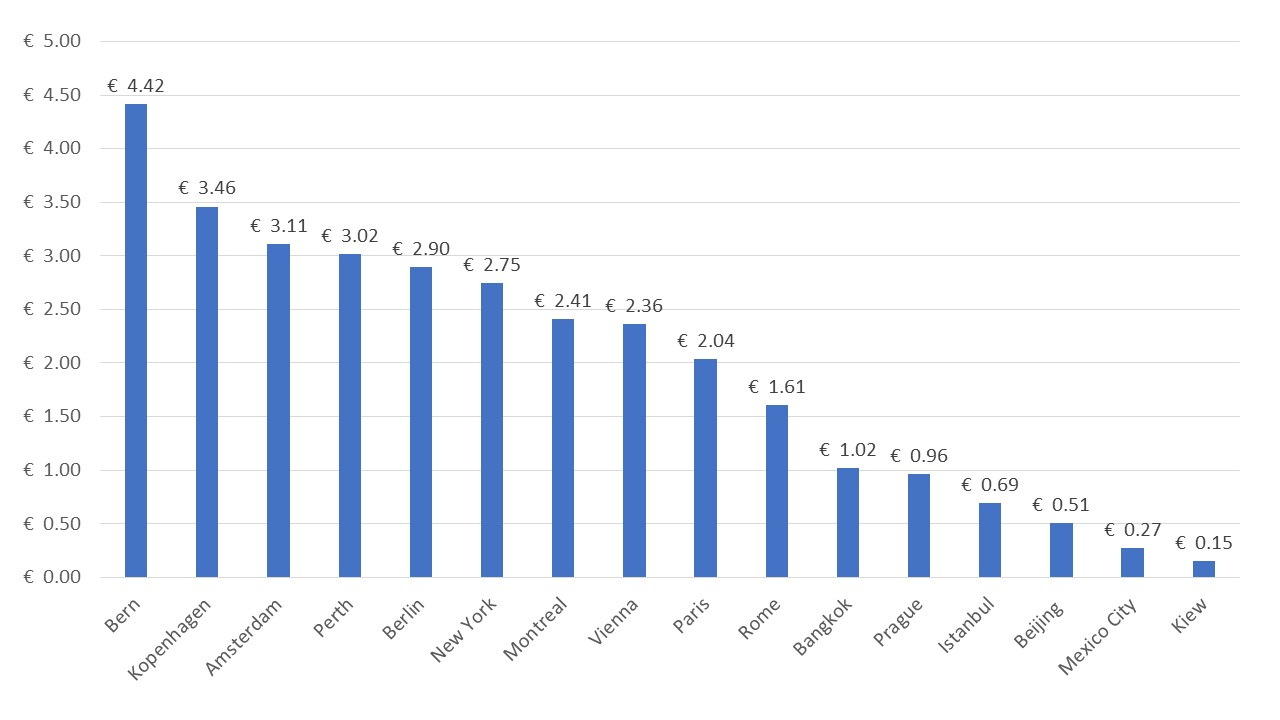
\includegraphics[width=1\linewidth]{image/tickets_prices} \caption{Prices for standard single tickets for local public transport in selected cities around the world  (statista.at, 2017)}\label{fig:unnamed-chunk-28}
\end{figure}

More and more cities nowadays offer public transport completely free of charge. The first experiments were already carried out in the 1960s. In the meantime, around 100 cities and towns around the world have introduced \href{https://freepublictransport.info/city/}{free public transportation} in one way or another. In some cities, only part of the public network is free, and in others, certain groups of the population, such as registered residents or pensioners, are allowed to ride for free. In Tallinn, the capital of Estonia, for example, residents have been able to ride the public transport system without a ticket since 2013. According to a study, this led to an increase in the proportion of people using public transport in the city from 55 to 63 percent (Cats et al., 2017). In 2018, they expanded the model to other parts of the country. Luxembourg, with a population of 626,000, is the first country to offer completely free public transport since 2020 (Yeung, 2021). In Dunkirk, France, public transportation has been free since 2018. A government-commissioned study concluded that eight months after the model was introduced, trips by bus increased by 65 percent during the week and 125 percent on weekends. Now some larger French cities are also experimenting with the idea. In Paris, free public transport for under-18s was introduced in 2020. In Strasbourg, the same policy will be implemented in September 2021. According to the Strasbourg government, this is a climate protection measure, as many of the 80,000 or so schoolchildren are currently taken to school by their parents. It is also intended to help socially disadvantaged families (who will save around 550 euros a year with two children) (Pallinger, 2021). In the Occitanie region of southern France (population around six million), a scheme has been introduced whereby 18- to 26-year-olds who travel by train at least 30 times a month will pay nothing, with the dual aim of helping young workers and reducing carbon emissions (Yeung, 2021).

The criticism of free public transportation is, on the one hand, that it would then be financed by higher taxes. Audrey Pulvar, the deputy mayor of Paris, wants to balance the financing with higher taxes on emission-intensive cars and large corporations like Amazon. In any case, the costs arising from traffic accidents, air pollution and congestion can be saved. According to Pulvar, these sums up to ten billion euros each year in the Paris region (Pallinger, 2021). Pulvar's proposals would first provide free transportation to youths under 18, students and job seekers in a phased rollout before expanding to all residents on weekends and then daily by 2026 (Yeung, 2021).

However, some people are sceptical about this idea. One of them is Kay Axhausen (professor for traffic planning at ETH Zurich). He argues that it can lead to an overload of the public transport and this leads to overcrowded and unreliable public transportation, and that customers are likely to be gone two days later. Prof.~Axhausen argues for better connections, easier transfers, prioritization at traffic signals, more bus lanes and changes to the route network to make public transport more attractive (Raaflaub, 2020).

Other criticisms include the rebound effect, which could lead to people traveling excessively by bus or tram, ultimately increasing traffic, emissions and urban sprawl, and fears that the quality of public transportation could deteriorate (more pollution from overcrowded buses and streetcars). Another point of criticism is that studies conclude that only a few people who previously travelled by car subsequently switched to free public transport. Most of the additional public transport users were mainly pedestrians, cyclists, and people who generally travelled less before, according to another study. The same is true in Tallinn where, although public transport has increased from 55 to 63 percent, the car share of traffic has only been reduced from 31 to 28 percent, while walking has fallen from 12 to 7 percent. According to the study, free public transportation would hardly change the mobility behaviour of car and motorcycle drivers (Pallinger, 2021). Another study in France concludes that while the measure would increase ridership by 6 to 10 percent, it would cost between €2.2 billion and €3.3 billion, the quality of service of the network would be compromised, car use would decrease by only 2 percent, and the impact on social equity would be limited because more than one million people in the region studied already benefit from free or reduced fares (Mabill \& Dugue, 2018). A greater change, according to some experts, could be brought about by measures such as higher parking fees or fuel prices. Instead of a general ticket exemption, poorer population groups could also be helped directly, for example by cheaper tickets for low income households. This would leave the government or the public transport company with most of the revenue from ticket sales (Pallinger, 2021). However, proponents of free public transport in France believe that the costs are overestimated and point to a tax (a so-called mobility tax) that is levied on all companies in France. This subsidizes collective transport and results in ticket sales accounting for only about 10-15\% of revenue in most cities. In the case of Dunkirk, this tax covered the cost of eliminating ticket prices, which represented 10\% of revenue (Yeung, 2021).

\hypertarget{relevant-initiatives-in-austria-23}{%
\subsection*{Relevant initiatives in Austria}\label{relevant-initiatives-in-austria-23}}
\addcontentsline{toc}{subsection}{Relevant initiatives in Austria}

Since 26th October 2021 in Austria ``KlimaTicket'' (climate ticket) is available for a standard price of €1.095 per year (€3 per day) giving access to all public transports in Austria.

\begin{itemize}
\tightlist
\item
  \href{https://www.klimaticket.at/en/}{BMK.gv.at}
\item
  \href{https://www.wienerlinien.at/web/wl-en/annual-pass}{Annual Pass Vienna}
\end{itemize}

\hypertarget{impacts-with-respect-to-sustainable-development-goals-sdgs-23}{%
\subsection*{Impacts with respect to Sustainable Development Goals (SDGs)}\label{impacts-with-respect-to-sustainable-development-goals-sdgs-23}}
\addcontentsline{toc}{subsection}{Impacts with respect to Sustainable Development Goals (SDGs)}

\begin{longtable}[]{@{}
  >{\centering\arraybackslash}p{(\columnwidth - 8\tabcolsep) * \real{0.2029}}
  >{\centering\arraybackslash}p{(\columnwidth - 8\tabcolsep) * \real{0.1884}}
  >{\centering\arraybackslash}p{(\columnwidth - 8\tabcolsep) * \real{0.2029}}
  >{\centering\arraybackslash}p{(\columnwidth - 8\tabcolsep) * \real{0.2029}}
  >{\centering\arraybackslash}p{(\columnwidth - 8\tabcolsep) * \real{0.2029}}@{}}
\toprule()
\begin{minipage}[b]{\linewidth}\centering
Impact level
\end{minipage} & \begin{minipage}[b]{\linewidth}\centering
Indicator
\end{minipage} & \begin{minipage}[b]{\linewidth}\centering
Impact direction
\end{minipage} & \begin{minipage}[b]{\linewidth}\centering
Goal description and number
\end{minipage} & \begin{minipage}[b]{\linewidth}\centering
Source
\end{minipage} \\
\midrule()
\endhead
Individual & Higher societal equity and public transport accessibility & \textbf{+} & Equality (\emph{5,10}) & Brown, 2018; Pallinger, 2021 \\
Individual & Reduction in sustainable transport modes (e.g.~walking) due to increased use of free public transport & \textbf{-} & Environmental sustainability (\emph{7,12,13,15}) & Pallinger, 2021 \\
Systemic & Reduced carbon emissions & \textbf{+} & Environmental sustainability (\emph{7,12,13,15}) & Yeung, 2021 \\
Systemic & Potentially excessive trips by public transport may decrease its quality & \textbf{-} & Sustainable economic development (\emph{8,11}) & Raaflaub, 2020 \\
\bottomrule()
\end{longtable}

\hypertarget{technology-and-societal-readiness-level-23}{%
\subsection*{Technology and societal readiness level}\label{technology-and-societal-readiness-level-23}}
\addcontentsline{toc}{subsection}{Technology and societal readiness level}

\begin{longtable}[]{@{}cc@{}}
\toprule()
TRL & SRL \\
\midrule()
\endhead
8-9 & 7-9 \\
\bottomrule()
\end{longtable}

\hypertarget{further-links-19}{%
\subsection*{Further links}\label{further-links-19}}
\addcontentsline{toc}{subsection}{Further links}

\begin{itemize}
\tightlist
\item
  \href{https://freepublictransport.info/city/}{Freepublictransport.info}
\item
  \href{https://orf.at/stories/3113027/}{Orf.at}
\end{itemize}

\hypertarget{references-23}{%
\subsection*{References}\label{references-23}}
\addcontentsline{toc}{subsection}{References}

\begin{itemize}
\tightlist
\item
  Krakow.pl (2021). Rodzaje biletów. Available at: \url{https://www.krakow.pl/14904,artykul,rodzaje_biletow.html}. {[}Accessed: 1st June 2021{]}
\item
  McKone, J. (2010). Time-Based Versus Distance-Based Fares. Available at: \url{https://thecityfix.com/blog/time-based-versus-distance-based-fares/\#}:\textasciitilde:text=Time\%2Dbased\%20systems\%20allow\%20passengers,a\%20set\%20amount\%20of\%20time.\&text=Distance\%2Dbased\%20systems\%20charge\%20higher,rides\%20that\%20cover\%20greater\%20distances. {[}Accessed: 1st June 2021{]}
\item
  Wiener Linien.at (2021). Ticket guide. Available at: \url{https://www.wienerlinien.at/eportal3/ep/channelView.do/pageTypeId/66533/channelId/-47643} {[}Accessed: 1st June 2021{]}
\item
  ADAC. (2019, June 19). ÖPNV-Preisvergleich 2019: Wo Tickets teuer und wo sie günstig sind \textbar{} ADAC. \url{https://www.adac.de/reise-freizeit/ratgeber/tests/oepnv-preise-vergleich/}
\item
  Brown, A. E. (2018). Fair fares? How flat and variable fares affect transit equity in Los Angeles. Case Studies on Transport Policy, 6(4), 765--773. \url{https://doi.org/10.1016/J.CSTP.2018.09.011}
\item
  Bull, O., Munoz, J. C., Silva, H. E. (2021). Impact of fare-free public transport on travel behavior: Evidence from a randomized controlled trial. Regional Science and Urban Economics. 86, 103616. \url{https://doi.org/10.1016/j.regsciurbeco.2020.103616}
\item
  Cats, O., Susilo, Y. O., \& Reimal, T. (2017). The prospects of fare-free public transport: evidence from Tallinn. Transportation, 44(5), 1083--1104. \url{https://doi.org/10.1007/s11116-016-9695-5}
\item
  Chalabianlou, R., Lawrence, A., \& Baxter, B. (2015). A review and assessment of fare capping as a passenger incentive mechanism for Australia and New Zealand. ATRF 2015 - Australasian Transport Research Forum 2015, Proceedings, October, 1--15.
\item
  El-Geneidy, A., Levinson, D., Diab, E., Boisjoly, G., Verbich, D., \& Loong, C. (2016). The cost of equity: Assessing transit accessibility and social disparity using total travel cost. Transportation Research Part A: Policy and Practice, 91, 302--316. \url{https://doi.org/10.1016/j.tra.2016.07.003}
\item
  Guzman, L. A., de la Hoz, D., \& Monzón, A. (2014). Optimal and Long-Term Dynamic Transport Policy Design: Seeking Maximum Social Welfare through a Pricing Scheme. International Journal of Sustainable Transportation, 8(4), 297--316. \url{https://doi.org/10.1080/15568318.2012.696772}
\item
  Hojski, D., Hazemali, D., Lep, M. (2022). The Analysis of the Effects of a Fare Free Public Transport Travel Demand Based on E-Ticketing. Sustainability. 14 (10), 5878. \url{https://doi.org/10.3390/su14105878}
\item
  Los Angeles County Metropolitan Transportation Authority. (2021). LA Metro Rider Relief. \url{https://www.metro.net/projects/rider_relief/}
\item
  Mabill, S., \& Dugue, H. (2018). Rapport du Comité sur la faisabilité de la gratuité des transports en commun en Île-de-France, leur financement et la politique de tarification. 2018--2019. \url{https://www.iledefrance-mobilites.fr/wp-content/uploads/2018/10/Rapport-Comité-sur-la-faisabilité-de-la-gratuité-des-transports-en-commun-en-Île-de-France-leur-financement-et-la-politique-de-tarification.pdf}
\item
  Martens, K. (2012). Justice in transport as justice in accessibility: Applying Walzer's ``Spheres of Justice'' to the transport sector. Transportation, 39(6), 1035--1053. \url{https://doi.org/10.1007/s11116-012-9388-7}
\item
  Pallinger, J. (2021, June 5). Was kostenlose Öffis bringen sollen - Zukunft - derStandard.de › Wissen und Gesellschaft. \url{https://www.derstandard.de/story/2000127046621/was-kostenlose-oeffis-bringen-sollen}
\item
  Raaflaub, C. (2020, February 27). Warum die Idee vom Gratis-ÖV in der Schweiz nicht ankommt - SWI swissinfo.ch. \url{https://www.swissinfo.ch/ger/verkehr-und-umweltschutz_warum-die-idee-vom-gratis-oev-in-der-schweiz-nicht-ankommt/45578796}
\item
  Rubensson, I., Susilo, Y., \& Cats, O. (2020). Is flat fare fair? Equity impact of fare scheme change. Transport Policy, 91, 48--58. \url{https://doi.org/10.1016/J.TRANPOL.2020.03.013}
\item
  San Francisco Municipal Transportation Agency. (2021, January). Lifeline Pass \textbar{} SFMTA. \url{https://www.sfmta.com/fares/lifeline-pass}
\item
  statista.at. (2017, April). ÖPNV - Preise für Standard-Einzeltickets weltweit 2017 \textbar{} Statista. \url{https://de.statista.com/statistik/daten/studie/168444/umfrage/preise-fuer-standard-einzeltickets-des-oepnv-in-ausgewaehlten-staedten/}
\item
  Streeting, M., \& Charles, P. (2006). Developments in transit fare policy reform. 29th Australasian Transport Research Forum, ATRF 06, 1--13.
\item
  Tomes, Z., Fitzova, H., Paril, V., Rederer, V., Kordova, Z., Kasa, M. (2022). Discounts and ree fares in long-dinstance public transport in central Europe. Case Studies on Transport Policy. 10, 507-517. \url{https://doi.org/10.1016/j.cstp.2022.01.011}
\item
  Wang, S., Liu, Y., \& Corcoran, J. (2021). Equity of public transport costs before and after a fare policy reform: An empirical evaluation using smartcard data. Transportation Research Part A: Policy and Practice, 144, 104--118. \url{https://doi.org/10.1016/J.TRA.2020.12.010}
\item
  Yeung, P. (2021, May 24). How France is testing free public transport - BBC Worklife. \url{https://www.bbc.com/worklife/article/20210519-how-france-is-testing-free-public-transport}
\item
  Yoh, A. C., Taylor, B. D., \& Gahbauer, J. (2016). Does Transit Mean Business? Reconciling Economic, Organizational, and Political Perspectives on Variable Transit Fares. Public Works Management and Policy, 21(2), 157--172. \url{https://doi.org/10.1177/1087724X15616816}
\item
  Zhao, P., \& Zhang, Y. (2019). The effects of metro fare increase on transport equity: New evidence from Beijing. Transport Policy, 74, 73--83. \url{https://doi.org/10.1016/J.TRANPOL.2018.11.009}
\end{itemize}

\hypertarget{maas}{%
\section{Mobility as a service (Maas)}\label{maas}}

\textbf{Updated: 13th July 2022}

\hypertarget{definition-24}{%
\subsection*{Definition}\label{definition-24}}
\addcontentsline{toc}{subsection}{Definition}

In line with the principle of ``\emph{using instead of owning}'', one goal of MaaS is to make mobility available as a service anytime and anywhere with a click on one or more online platforms or apps. These digital MaaS platforms or apps should link information, booking and payment of mobility offers from different service providers and thus enable the offer of integrated mobility packages. Users should have the freedom to choose between different physical forms of mobility (Neumann \& Rauch, 2021):

\begin{itemize}
\tightlist
\item
  public transport such as train, bus, rapid transit, tram and metro
\item
  private services such as taxis
\item
  services for car, ride, (e-)bike, (e-)scooter sharing or fixed route taxis
\item
  volunteer-run community buses
\item
  aircrafts and ships
\item
  (in the future) autonomous, driverless vehicles
\end{itemize}

MaaS solutions can be built up in stages. The first stage consists of a bundling of information from different providers so that all available mobility offers are displayed for the entire journey from start to destination. Stage two includes planning routes according to customers' priorities and the possibility to book and pay for all means of transport used for the journey at once. In addition, real-time information for the route is included, such as changes in journey and waiting times due to unforeseen events - such as accidents or weather conditions -- as well as continuous notifications about alternative options. Stage three consists of a mobility guarantee by means of a customised mobility package based on personal needs and preferences, e.g.~in the form of a monthly subscription (Neumann \& Rauch, 2021).
The aim of MaaS is to provide an alternative to the private use of cars, thus equally convenient, even cheaper, but more sustainable (Maas Alliance, 2015). The theory of MaaS opens up new business areas and enables mobility service providers to increase their customer base. The usage data generated by the ongoing operation can help to get to know customers better and thus to work more efficiently, as it would be easier to plan the orientation and distribution of the services. A well-functioning MaaS system requires the willingness of private and public mobility providers to cooperate with each other and with the platform operators (MaaS providers) (Neumann \& Rauch, 2021). Moreover, it relies heavily on availability of high-quality data. To enforce safe and secure real-time access to data , is equally important as ensuring the clarity regarding liabilities of parties with principal control over the data (Maas Alliance, 2015). The first step towards MaaS is the harmonization of data, supported by appropriate regulations and standards (Maas Alliance, 2015). In Austria, both researchers and mobility service providers are researching how to best implement MaaS. One example is the ULTIMOB research project.

\hypertarget{key-stakeholders-24}{%
\subsection*{Key stakeholders}\label{key-stakeholders-24}}
\addcontentsline{toc}{subsection}{Key stakeholders}

\begin{itemize}
\tightlist
\item
  \textbf{Affected}: Customers/Users
\item
  \textbf{Responsible}: Transport service providers and public transport operators, MaaS operators and integrators, IT system providers, city councils, local, regional and national authorities
\end{itemize}

\hypertarget{current-state-of-art-in-research-24}{%
\subsection*{Current state of art in research}\label{current-state-of-art-in-research-24}}
\addcontentsline{toc}{subsection}{Current state of art in research}

In order to support the cooperation between private and public mobility providers as well as platform operators (MaaS providers), the legal and organizational framework conditions as well as standards for a secure and fair exchange of data should be created at European and Austrian level (Neumann \& Rauch, 2021).
In 2015 the MaaS Alliance, a public-private partnership, working to establish foundations for a common approach to MaaS, was founded, with the main goal, to facilitate a single, open market and full deployment of MaaS services (Maas Alliance, 2015).
The research and development project \emph{MaaS4EU}, which is funded by the Horizon2020 research and innovation programme, brings together 17 partners from several sectors and backgrounds to provide viable evidence and solutions about the MaaS concept. The project aims to remove barriers and enable a cooperative and interconnected EU single transport market for the MaaS concept, by addressing the four pillars:

\begin{enumerate}
\def\labelenumi{(\arabic{enumi})}
\tightlist
\item
  business models
\item
  end-users
\item
  technology
\item
  policy
\end{enumerate}

Therefore, the holistic \emph{MaaS4EU} solutions are demonstrated and validated in real life via Living Labs in Greater Manchester (UK), Luxembourg-Germany, and Budapest (Hungary) (MaaS4EU, 2017). In summmary, current research is mainly working on the development of different MaaS app/platform prototypes, that will offer a multimodal travel solution. One example is the project \emph{TrønderMaaS} of Marinelli et al.~(2020) who is operating a full-scale pilot test in the Trondheim-Stjørdal region, Norway.

Literature reviews reveal a reduction in vehicle kilometres travelled, increased trip awareness, reduced parking, reduced vehicle ownership and improved social equity through implementation of MaaS. Barriers of MaaS supply are public private cooperation, business support, service coverage, shared vision and data/cyber security. On the demand side, barriers include its lack of appeal to older generations, public transport and private vehicle users, the attractiveness of the digital platform and the user willingness-to-pay (Buttler et al., 2021). Feneri et al.~(2020) found, that it is not only the price but the combination of monthly fees and the discounts for various transportation modes within a specific MaaS bundle that increases or decreases its use. Hensher et al.~(2021) provided similar findings that MaaS programs have the ability to increase or decrease the use of private cars, depending on the offered bundles. This suggests a reasoned approach, evaluated for each case separately, to be in compliance with the sustainability goals.

ITS Austria presents three levels of readiness for MaaS miA (Mobility as a Service made in Austria) (ITS Austria, 2019):

\begin{itemize}
\tightlist
\item
  Level 0: no integration and coordination of mobility services/offers
\item
  Level 1: 1a) integration of information, 1b) integration of offers
\item
  Level 2: contractible offers (fusion of large parts of relevant mobility offers)
\item
  Level 3: integration of agreements (mobility package and guarantee)
\end{itemize}

\hypertarget{current-state-of-art-in-practice-24}{%
\subsection*{Current state of art in practice}\label{current-state-of-art-in-practice-24}}
\addcontentsline{toc}{subsection}{Current state of art in practice}

The first pilot trial in Sweden started in 2013 with the plattform Ubi-Go. In April 2019 the App was launched and is looking for franchise partners since 2020 while Finland started its first MaaS platform in 2015, named whim, being the first commercially used combined mobility platform. Whim is now available in countries like Switzerland, Japan, Austria, Belgium and the UK (Whim, 2022; Ubi-Go, 2022).

In 2019 Berlin's public transport authority \emph{Berliner Verkehrsbetriebe (BVG)} invented and implemented together with the Lithuanian start-up and MaaS solution leader \emph{Trafi} the mobility app called \emph{Jelbi}, which counts as the world's most extensive Mobility as a Service-solution (Rastenytė, 2020). The app covers assistance planning and routes discovery, real-time public transport information and shared mobility vehicle location and availability, a streamlined payment solution for any integrated mobility service, as well as the possibility to compare the duration and cost of each trip (Rastenytė, 2020).

In 2020, Switzerland followed and integrated an app called \emph{yumuv}. \emph{Swiss Federal Railways SBB CFF FFS, PTOs of Verkehrsbetriebe Zürich, Basler Verkehrs-Betriebe (BVB)}, and \emph{BERNMOBIL} cooperated also with the start-up \emph{Trafi} and managed to create the first regional MaaS with subscriptions (Trafi Ltd., 2020).

On national level there is \href{https://wegfinder.at/}{wegfinder} (in all of Austria), \href{https://www.wienerlinien.at/wienmobil-app}{Wien Mobil} for the city of Vienna and \href{https://www.tim-oesterreich.at/graz/}{tim-App} in Graz and Linz.

\hypertarget{relevant-initiatives-in-austria-24}{%
\subsection*{Relevant initiatives in Austria}\label{relevant-initiatives-in-austria-24}}
\addcontentsline{toc}{subsection}{Relevant initiatives in Austria}

\begin{itemize}
\tightlist
\item
  \href{https://www.austriatech.at/assets/Uploads/Publikationen/PDF-Dateien/29fc02ada2/MaaS-miA_english_102019_web.pdf}{AustriaTech.at}
\item
  \href{https://maas-ready.at}{maas-ready.at}
\item
  \href{https://www.ultimob.at}{ultimob.at}
\item
  \href{https://www.tim-oesterreich.at/graz/}{tim-oesterreich.at}
\item
  \href{https://wegfinder.at/}{wegfinder.at}
\item
  \href{https://www.wienerlinien.at/eportal3/ep/channelView.do/pageTypeId/66526/channelId/-3600060}{wienerlinien.at}
\item
  \href{https://www.wienerlinien.at/wienmobil-app}{wienmobil-app}
\item
  \href{https://anachb.vor.at/}{anachb.vor.at}
\item
  \href{https://www.interregeurope.eu/find-policy-solutions/stories/primaas-enabling-mobility-as-a-service}{Interreg Europe: PriMaas}
\end{itemize}

\hypertarget{impacts-with-respect-to-sustainable-development-goals-sdgs-24}{%
\subsection*{Impacts with respect to Sustainable Development Goals (SDGs)}\label{impacts-with-respect-to-sustainable-development-goals-sdgs-24}}
\addcontentsline{toc}{subsection}{Impacts with respect to Sustainable Development Goals (SDGs)}

\begin{longtable}[]{@{}
  >{\centering\arraybackslash}p{(\columnwidth - 8\tabcolsep) * \real{0.2029}}
  >{\centering\arraybackslash}p{(\columnwidth - 8\tabcolsep) * \real{0.1884}}
  >{\centering\arraybackslash}p{(\columnwidth - 8\tabcolsep) * \real{0.2029}}
  >{\centering\arraybackslash}p{(\columnwidth - 8\tabcolsep) * \real{0.2029}}
  >{\centering\arraybackslash}p{(\columnwidth - 8\tabcolsep) * \real{0.2029}}@{}}
\toprule()
\begin{minipage}[b]{\linewidth}\centering
Impact level
\end{minipage} & \begin{minipage}[b]{\linewidth}\centering
Indicator
\end{minipage} & \begin{minipage}[b]{\linewidth}\centering
Impact direction
\end{minipage} & \begin{minipage}[b]{\linewidth}\centering
Goal description and number
\end{minipage} & \begin{minipage}[b]{\linewidth}\centering
Source
\end{minipage} \\
\midrule()
\endhead
Individual & Facilitated accessibility to transport & \textbf{+} & Equality (\emph{5,10}) & Gudonavicius, 2020 \\
Individual & Use of active transport modes increased/Fuel consumption decreased & \textbf{+} & Environmental sustainability (\emph{7,12,13,15}) & Gudonavicius, 2020 \\
Individual & Higher accessibility \& faster travel time & \textbf{+} & Sustainable economic development (\emph{8,11}) & Gudonavicius, 2020; Marinelli et al., 2020 \\
Individual & Use of digitalized transport & \textbf{+} & Innovation \& Infrastructure (\emph{9}) & Gudonavicius, 2020; Marinelli et al., 2020 \\
Systemic & Transport safety increased/Collision rates reduced & \textbf{+} & Health \& Wellbeing (\emph{3}) & Gudonavicius, 2020; Marinelli et al., 2020 \\
Systemic & Emissions rate reduced & \textbf{+} & Environmental sustainability (\emph{7,12,13,15}) & Gudonavicius, 2020 \\
Systemic & Traffic efficiency & \textbf{+} & Sustainable economic development (\emph{8,11}) & Gudonavicius, 2020 \\
Systemic & Efficiency of transport systems, increased resilience through real-time data & \textbf{+} & Innovation \& Infrastructure (\emph{9}) & Marinelli et al., 2020 \\
Systemic & Collaborations of private and public sectors \& global partnerships & \textbf{+} & Partnership \& collaborations (\emph{17}) & Gudonavicius, 2020; Marinelli et al., 2020 \\
\bottomrule()
\end{longtable}

\hypertarget{technology-and-societal-readiness-level-24}{%
\subsection*{Technology and societal readiness level}\label{technology-and-societal-readiness-level-24}}
\addcontentsline{toc}{subsection}{Technology and societal readiness level}

\begin{longtable}[]{@{}cc@{}}
\toprule()
TRL & SRL \\
\midrule()
\endhead
3-7 & 5-7 \\
\bottomrule()
\end{longtable}

\hypertarget{open-questions-22}{%
\subsection*{Open questions}\label{open-questions-22}}
\addcontentsline{toc}{subsection}{Open questions}

\begin{enumerate}
\def\labelenumi{\arabic{enumi}.}
\tightlist
\item
  How can a sustainability transformation be reached through MaaS and what circumstances does it require?
\item
  How can data protection be ensured when using MaaS?
\item
  How fast is MaaS going to be implemented?
\item
  How can bureaucratic hurdles be overcome in a timely manner?
\end{enumerate}

\hypertarget{further-links-20}{%
\subsection*{Further links}\label{further-links-20}}
\addcontentsline{toc}{subsection}{Further links}

\begin{itemize}
\tightlist
\item
  \href{https://maas-alliance.eu/wp-content/uploads/sites/7/2017/09/MaaS-WhitePaper_final_040917-2.pdf}{maas-alliance.eu}
\item
  \href{https://www.trafi.com}{trafi.com}
\item
  \href{https://www.jelbi.de}{jelbi.de}
\item
  \href{https://www.ubigo.me/en/about-ubigo}{ubigo.me}
\item
  \href{http://www.maas4eu.eu}{maas4eu.eu}
\end{itemize}

\hypertarget{references-24}{%
\subsection*{References}\label{references-24}}
\addcontentsline{toc}{subsection}{References}

\begin{itemize}
\tightlist
\item
  Butler, L., Yigitcanlar, T., Paz, A. (2021). Barriers and risks of Mobility-as-a-Service (MaaS) adoption in cities: A systematic review of the literature. Cities. 109, 103036. \url{https://doi.org/10.1016/j.cities.2020.103036}
\item
  Feneri, A-M., Rasouli, S., Timmermans, H.J.P. (2020). Modeling the effect of Mobility-as-a-Service on mode choice decisions. Transportation Letters. 14 (4), 324-331. \url{https://doi.org/10.1080/19427867.2020.1730025}
\item
  Fluidtime (2022). Ubi-Go App. Available at: \url{https://www.fluidtime.com/en/ubigo/} {[}Accessed: 11th July 2022{]}
\item
  Gudonavičius, M. (2020). Unjamming Urban Mobility: How Mobility-as-a-Service Can Replace Personal Cars. \url{https://www.trafi.com/wp-content/uploads/2020/08/unjamming-urban-mobility.pdf}
\item
  Maas Alliance. (2015). White Paper: Guidelines \& Recommendations to create the foundation for a thriving MaaS Ecosystem. 32(2), 1--27. \url{https://maas-alliance.eu/wp-content/uploads/sites/7/2017/09/MaaS-WhitePaper_final_040917-2.pdf}
\item
  Hensher, D., Ho, C. Q., Reck, D. J. (2021). Mobility as a service and private car use: Evidence from the Sydney MaaS trial. Transportation Research Part A: Policy and Practice. 145, 17-33. \url{https://doi.org/10.1016/j.tra.2020.12.015}
\item
  MaaS4EU. (2017, October). Launch of MaaS4EU project. \url{http://www.maas4eu.eu/wp-content/uploads/2017/10/MaaS4EU-Launch-Press-Release.pdf}
\item
  Marinelli, G., Nordfjærn, Ö. S., Aarseth, W., \& Pitera, K. (2020). Introducing TrønderMaaS: investigating business models, sustainability and users' acceptance of a MaaS system in Stjørdal and Trondheim region, Norway.
\item
  Neumann, A., \& Rauch, A. (2021). Maas Ready. \url{https://maas-ready.at/allgemein\#Grundidee}
\item
  Rastenytė, J. (2020, April 24). BVG Jelbi -- Case Study: World's Most Extensive MaaS in Berlin -- Trafi. \url{https://www.trafi.com/bvg-jelbi-maas-berlin/}
\item
  Trafi Ltd.~(2020). yumuv -- Regional MaaS with subscriptions in Switzerland -- Trafi. \url{https://www.trafi.com/yumuv/}
\item
  Whim-App (2022). Available at: \url{https://whimapp.com/} {[}Accessed: 11th July 2022{]}
\end{itemize}

\hypertarget{p_r}{%
\section{Park and ride}\label{p_r}}

\textbf{Updated: 1st August 2022}

\hypertarget{synonyms-21}{%
\subsection*{Synonyms}\label{synonyms-21}}
\addcontentsline{toc}{subsection}{Synonyms}

\emph{P\&R, P and R, P+R}

\hypertarget{definition-25}{%
\subsection*{Definition}\label{definition-25}}
\addcontentsline{toc}{subsection}{Definition}

Some of the main challenges the world is currently facing are related to population growth and urbanisation. The massive growth of cities has created major transport challenges that manifest themselves in traffic congestion in urban areas, especially in city centres. Many of the efforts to reduce congestion attempt to increase vehicle occupancy by inducing a shift from single occupancy vehicles (SOVs) to multiple occupancy vehicles or encouraging use of various transit modes. One example of such effort are park-and-ride facilities which attempt to reduce car use and increase road efficiency.
Park-and-ride facilities are usually located in peri-urban areas in a proximity to bus or train station to allow drivers coming from suburban and rural areas to park their cars and transfer to public transport to reach urban destinations. Park-and-ride facilities, introduced in England in the 1970s, appear to offer a simple and cost-effective alternative to building new roads. These facilities are usually accompanied by good public transport services to urban areas (Katoshevski-Cavari, Bak and Shiftan, 2018).

\hypertarget{key-stakeholders-25}{%
\subsection*{Key stakeholders}\label{key-stakeholders-25}}
\addcontentsline{toc}{subsection}{Key stakeholders}

\begin{itemize}
\tightlist
\item
  \textbf{Affected}: Car drivers coming from suburban and rural areas
\item
  \textbf{Responsible}: National Governments, Communal Governments, City governments, Parking Companies
\end{itemize}

\hypertarget{current-state-of-art-in-research-25}{%
\subsection*{Current state of art in research}\label{current-state-of-art-in-research-25}}
\addcontentsline{toc}{subsection}{Current state of art in research}

In terms of P\&R research, existing publications address topics such as the optimal location problem of P\&R facilities, the relationship between private vehicle use patterns and the number and density of P\&R facilities in a city, the empirical study of P\&R facility use patterns, the study of P\&R motives and air quality standards in Europe, the influence of P\&R facilities on vehicle kilometres travelled, the analysis of travellers' stated intention to use parking and cycling facilities (P+R, B+R), empirical analysis of P\&R facility choice behaviour, attitude surveys of P\&R and non-P\&R users and the influence of multimodal information on the use of P\&R (Gan and Ye, 2018).
Studies show that some public transport users were attracted to switch to multiple modes of transport (i.e.~park-and-ride), which increased the number of car trips. Nonetheless, additional car trips are made in non-congested areas, thus contributing to traffic relief (Katoshevski-Cavari, Bak and Shiftan, 2018).
The exact effects of P\&R are controversial. Some studies have confirmed that P\&R facilities can encourage the use of public transport, relieve urban traffic and reduce car emissions in city centres. Other studies pointed to possible counter-effects of P\&R. The reduction of congestion in city centres might encourage motorists to use their cars in the city again, as accessibility has increased, and motorists travelling to the city centre via P\&R facilities might travel some extra kilometres to reach the P\&R facility. The exact weight of these negative externalities is still debatable (and will vary from place to place), as is the direct net benefit of P\&R on car traffic in the city area as a whole. However, it is undisputed that well-used P\&R facilities directly reduce car traffic in the city centre (Dijk and Montalvo, 2011), especially if the travel behaviour in a certain area was well-researched which is a key element to be able to convince travellers to switch to a multi-modal travel (Memon et al., 2021). A recent study showed, based on an agent simulation system, that compared with reducing the public transport fares, reducing the waiting times can attract car travellers to choose park and ride while the co-existence of a reservation scheme can reduce cruising and improve traffic environment (Zhenyu et al., 2022). Further, Bruck and Soteropoulos (2021) stated, that under future circumstances of (shared) automated vehicles, Park and Ride facilities might need to be transformed to mobility hubs, to make it possible to accommodate future autonomous shuttle fleets.

\hypertarget{current-state-of-art-in-practice-25}{%
\subsection*{Current state of art in practice}\label{current-state-of-art-in-practice-25}}
\addcontentsline{toc}{subsection}{Current state of art in practice}

Parking management has evolved greatly in Europe over the last decades, and P\&R has emerged as one of the newest elements of urban parking management. Virtually all urban areas are facing growing parking demand. More parking spaces lead to growing problems of urban congestion and pollution from traffic. Many cities have responded with policies aimed at improving the utilisation of existing infrastructure (e.g.~through pricing or automatic display of parking capacity) and building new infrastructure at structural bottlenecks. The typical development of urban parking policies can be presented in seven phases (Dijk and Montalvo, 2011):

\begin{enumerate}
\def\labelenumi{\arabic{enumi}.}
\tightlist
\item
  \textbf{No parking measures}: This phase is sustainable until the level of parked cars has a negative impact on the attractiveness and quality of the area.
\item
  \textbf{Regulation and control of parking}: This means banning parking in some streets.
\item
  \textbf{Time restrictions (free of charge)}: This leads to more efficient use of available space through increased turnover of cars.
\item
  \textbf{Paid parking}: Parking tariffs are used as a key to control the use of parking spaces.
\item
  \textbf{Resident parking schemes}: Overflow of parkers into neighbouring areas (often residential) requires resident parking regulations.
\item
  \textbf{P\&R facilities}: These are being developed as an alternative or supplement to parking provision in the town centre.
\item
  \textbf{Mobility management}: It includes various activities to coordinate the combination of private and public transport to create an acceptable mobility chain for travellers.
\end{enumerate}

Moreover, the results of a survey show that a quarter of the cities in Europe are intensively engaged in P + R development, while about 50\% of them is moderately engaged. Geographically, it shows that cities in north-western Europe have a higher level of engagement than cities in southern and eastern Europe. Furthermore, the understanding of P\&R in European cities is strongly different, revealing current beliefs about P\&R.
Park-and-Ride is certainly not the only transport policy initiative in the city to improve accessibility and quality of life in the city. Most cities apply combination of measures. P\&R is valued as part of such a package, but not seen as the perfect package. Most cities consider P\&R as a ``Plan B'' (Dijk and Montalvo, 2011).
In Germany, some P\&R facilities were tested by the ADAC. Many P\&R facilities had deficiencies - most of them were missing equipment features:

\begin{itemize}
\tightlist
\item
  The testers hardly found any video surveillance, and forecasts of occupancy on the Internet were also scarce;
\item
  No car park had continuous footpaths and safe separation between pedestrians and cars;
\item
  In 25\% of facilities, there were not enough parking spaces available, showing a gap between supply and demand.
\item
  Some of the public transport services were also unsatisfactory, with too long waiting/transfer time. The likelihood of choosing P + R facility decreases with longer public transport travel and waiting times (Islam et al., 2015).
\end{itemize}

The facilities scored best in the category of information and prices. Two thirds had clear signage and provided comprehensible information on their websites about location, size and prices. Two of them were particularly positive: they published online forecasts of available parking spaces so that drivers could estimate in advance when parking spaces would be available. The Bremen-Burg P\&R facility offered additional useful service: a display board showed free parking spaces and the departure times of the next two trains.
In passenger traffic, commuters do not want to wait long for their train. The frequency of public transport therefore has a significant impact on whether a P\&R facility is accepted at all. In one third of the facilities, the connection to the public transport network (travel time ratio, frequency, routes to the station) was poor or very poor.
The testers checked lighting, digital or personal surveillance, recognisable separation between parking spaces and the roadway, and whether the transition from the car park to the station was safe. Overall, the study showed that current level of safety is unsatisfactory.

Recommendations for operators:

\begin{itemize}
\tightlist
\item
  Provide information about P\&R facilities on the Internet
\item
  Pave, regularly maintain and clean the entire P\&R facility - including temporary parking spaces.
\item
  Make parking spaces at least 2.50 metres wide so that users can get on and off without difficulty.
\item
  Keep footpaths short and safely separated from the roadway, clearly mark parking spaces and regularly tighten faded markings.
\item
  Provide charging infrastructure for electric vehicles
\item
  In multi-storey car parks, provide more security through video surveillance, good visibility, functioning emergency calls and comprehensive lighting
\item
  Manage P\&R facilities at high occupancy rates (user fees, parking time restrictions) in order to avoid misuse.
\end{itemize}

Recommendations for municipalities \& public transport:

\begin{itemize}
\tightlist
\item
  Planning on a large scale and regionally already when developing areas for P\&R facilities.
\item
  Where demand is particularly high and space is available, create more P\&R spaces - possibly also by building parking decks.
\item
  Ensure good public transport connections to the city centre with short intervals.
\item
  Avoid large jumps in fares, if necessary integrate selected P\&R facilities into cheaper fare groups.
\item
  Combine Bike+Ride and P\&R facilities to make it possible for residents from the immediate vicinity to reach the facility by bicycle instead of by car (Luca and Dommnich, 2018).
\end{itemize}

\hypertarget{relevant-initiatives-in-austria-25}{%
\subsection*{Relevant initiatives in Austria}\label{relevant-initiatives-in-austria-25}}
\addcontentsline{toc}{subsection}{Relevant initiatives in Austria}

ÖBB is investing 700 million euros in the expansion of infrastructure in the eastern region in the next years, staring in 2021. Two thirds of rail passengers in Austria travel in Lower Austria, Vienna and Burgenland, where lines are being extended, stations renovated and new park-and-ride facilities built (Frey, 2021). In Vienna, Lower Austria and Burgenland, more than 40,000 parking spaces are available at over 200 Park/B+R facilities for easy transfers. In Vienna, most P\&R facilities charge a small fee of € 3.60 per day. In Lower Austria and Burgenland, the use of P\&R facilities is free of charge for public transport passengers (VOR.at, n.d.), while in Vienna, holders of a valid monthly or yearly public transport ticket get reduced monthly and yearly P\&R tickets (WiPark.at, 2022). Further, in May 2022 a new access system at the P+R facility in St.~Pölten was implemented, which allows easier access for all owners of permanent tickets due to number plate recognition at the entrance and exit (Schrefl, 2022).

\begin{itemize}
\tightlist
\item
  \href{https://www.wien.info/de/reiseinfos/anreise/parkgaragen}{wien.info}
\item
  \href{https://www.wien.gv.at/verkehr/parken/garagen/}{wien.gv.at}
\item
  \href{https://www.derstandard.at/story/2000106482985/volle-park-and-ride-plaetze-frustrieren-wien-pendler}{derstandard.at}
\item
  \href{https://orf.at/stories/3151437/}{orf.at}
\item
  \href{https://noe.orf.at/stories/3030525/}{noe.orf.at}
\item
  \href{https://www.parken.at/}{parking in Austria}
\end{itemize}

\hypertarget{impacts-with-respect-to-sustainable-development-goals-sdgs-25}{%
\subsection*{Impacts with respect to Sustainable Development Goals (SDGs)}\label{impacts-with-respect-to-sustainable-development-goals-sdgs-25}}
\addcontentsline{toc}{subsection}{Impacts with respect to Sustainable Development Goals (SDGs)}

\begin{longtable}[]{@{}
  >{\centering\arraybackslash}p{(\columnwidth - 8\tabcolsep) * \real{0.2029}}
  >{\centering\arraybackslash}p{(\columnwidth - 8\tabcolsep) * \real{0.1884}}
  >{\centering\arraybackslash}p{(\columnwidth - 8\tabcolsep) * \real{0.2029}}
  >{\centering\arraybackslash}p{(\columnwidth - 8\tabcolsep) * \real{0.2029}}
  >{\centering\arraybackslash}p{(\columnwidth - 8\tabcolsep) * \real{0.2029}}@{}}
\toprule()
\begin{minipage}[b]{\linewidth}\centering
Impact level
\end{minipage} & \begin{minipage}[b]{\linewidth}\centering
Indicator
\end{minipage} & \begin{minipage}[b]{\linewidth}\centering
Impact direction
\end{minipage} & \begin{minipage}[b]{\linewidth}\centering
Goal description and number
\end{minipage} & \begin{minipage}[b]{\linewidth}\centering
Source
\end{minipage} \\
\midrule()
\endhead
Individual & Reduced initial congestion in city centres & \textbf{\textasciitilde{}} & Health \& Wellbeing (\emph{3}) & Dijk \& Montalvo, 2011 \\
Individual & Increased access to public transport \& multimodal travel & \textbf{+} & Equality (\emph{5,10}) & Macioszek \& Kurek, 2020 \\
Individual & Low cost or free of charge & \textbf{+} & Sustainable economic development (\emph{8,11}) & VOR.at, n.d. \\
Systemic & Ambiguous impact on emissions & \textbf{\textasciitilde{}} & Environmental sustainability (\emph{7,12-13,15}) & Moore et al., 2019; ITF, n.d. \\
Systemic & New infrastructure built & \textbf{+} & Innovation \& Infrastructure (\emph{9}) & Frey, 2021 \\
\bottomrule()
\end{longtable}

\hypertarget{technology-and-societal-readiness-level-25}{%
\subsection*{Technology and societal readiness level}\label{technology-and-societal-readiness-level-25}}
\addcontentsline{toc}{subsection}{Technology and societal readiness level}

\begin{longtable}[]{@{}cc@{}}
\toprule()
TRL & SRL \\
\midrule()
\endhead
8-9 & 7-9 \\
\bottomrule()
\end{longtable}

\hypertarget{open-questions-23}{%
\subsection*{Open questions}\label{open-questions-23}}
\addcontentsline{toc}{subsection}{Open questions}

\begin{enumerate}
\def\labelenumi{\arabic{enumi}.}
\tightlist
\item
  How to encourage non-commuters to use P\&R?
\item
  How will demand for P\&R parking change over time, especially with the rapid changes associated with the introduction of autonomous vehicles?
\item
  What is the potential of P\&R in facilitating multimodal transport at the advent of integrated travel apps?
\end{enumerate}

\hypertarget{further-links-21}{%
\subsection*{Further links}\label{further-links-21}}
\addcontentsline{toc}{subsection}{Further links}

\begin{itemize}
\tightlist
\item
  \href{https://www.itf-oecd.org/policy/park-and-ride-facilities}{itf-oecd.org}
\item
  \href{http://www.parkeninwien.at/en/Park-and-Ride.html}{parkeninwien.at}
\item
  \href{https://www.stadt-wien.at/wien/parken-in-wien/park-ride-parkhaeuser-im-ueberblick.html}{stadt-wien.at}
\end{itemize}

\hypertarget{references-25}{%
\subsection*{References}\label{references-25}}
\addcontentsline{toc}{subsection}{References}

\begin{itemize}
\tightlist
\item
  Bruck, E. M., Soteropoulos, A. (2021). Traffic-land use compatibility and street design impacts of automated driving in Vienna, Austria. The Journal of Transport and Land Use. 15, 1. 137-163. \url{http://dx.doi.org/10.5198/jtlu.2022.2089}
\item
  Dijk, M., \& Montalvo, C. (2011). Policy frames of Park-and-Ride in Europe. Journal of Transport Geography, 19(6), 1106--1119. \url{https://doi.org/10.1016/j.jtrangeo.2011.05.007}
\item
  Frey, F. (2021, January 6). ÖBB: 700 Mio. Euro für Infrastrukturausbau - noe.ORF.at. \url{https://noe.orf.at/stories/3083619/}
\item
  Gan, H., \& Ye, X. (2018). Will commute drivers switch to park-and-ride under the influence of multimodal traveler information? A stated preference investigation. Transportation Research Part F: Traffic Psychology and Behaviour, 56, 354--361. \url{https://doi.org/10.1016/j.trf.2018.05.015}
\item
  Islam, S. T., Liu, Z., Sarvi, M., \& Zhu, T. (2015). Exploring the mode change behavior of park-and-ride users. Mathematical Problems in Engineering, 2015.
\item
  ITF. (n.d.) Park and ride facilities. Available at: \url{https://www.itf-oecd.org/policy/park-and-ride-facilities} {[}Accessed: 3 March 2021{]}.
\item
  Katoshevski-Cavari, R., Bak, N., \& Shiftan, Y. (2018). Would free park-and-ride with a free shuttle service attract car drivers? Case Studies on Transport Policy, 6(2), 206--213. \url{https://doi.org/10.1016/j.cstp.2018.05.001}
\item
  Luca, K., \& Dommnich, B. (2018, August 6). 60 P+R-Anlagen im Test \textbar{} ADAC. \url{https://www.adac.de/reise-freizeit/ratgeber/tests/park-ride/}
\item
  Macioszek, E., \& Kurek, A. (2020). The use of a park and ride system---A case study based on the city of Cracow (Poland). Energies, 13(13), 3473.
\item
  Memon, I. A., Kalwar, S., Sahito, N., Talpur, M. H., Chandio, I. A., Napiah, M., Tayyeb, H. (2021). Mode Choice Modeling to Shift Car Travellers towards Park and Ride Service in the City centre of Karachi. Sustainability. 13(10), 5638. \url{https://doi.org/10.3390/su13105638}
\item
  Moore, A. M., Curran, S. J., Lapsa, M. V., \& Bittler, A. D. (2019). Geoanalysis of park-and-ride facilities for future laboratory-wide commuting program. Transportation Research Interdisciplinary Perspectives, 3, 100025. \url{https://doi.org/10.1016/j.trip.2019.100025}
\item
  Schrefl, K. (2022). MeinBezirk.at: Park \& Ride Anlagen bekommen ein neues Zufahrtssystem. Available at: \url{https://www.meinbezirk.at/st-poelten/c-lokales/park-und-ride-anlagen-bekommen-ein-neues-zufahrtssystem_a5280277} {[}Accessed: 19 July 2022{]}
\item
  VOR.at. (n.d.). Park/Bike+Ride - VOR. Available at: \url{https://www.vor.at/mobil/parkbike-ride/} {[}Accessed: 26 February 2021{]}
\item
  WiPark.at. (2022). Park and Ride (P+R) -- Ihr Parkplatz an der U-Bahn oder S-Bahn. Available at: \url{https://www.wipark.at/parkprodukte/angebote/park-and-ride} {[}Accessed: 19 July 2022{]}
\item
  Zhenyu, M., Daqin, W., Wenchao, D., Dianhai, W., Dongfang, M. (2022). Multi-Agent Simulation for Multi-Mode Travel Policy to Improve Park and Ride Efficiency. Available at SSRN: \url{https://dx.doi.org/10.2139/ssrn.4151394}
\end{itemize}

\hypertarget{contactless_cards}{%
\section{Contactless public transport cards}\label{contactless_cards}}

\textbf{Updated: 1st August 2022}

\hypertarget{synonyms-22}{%
\subsection*{Synonyms}\label{synonyms-22}}
\addcontentsline{toc}{subsection}{Synonyms}

\emph{Contactless smart card, smart card ticketing}

\hypertarget{definition-26}{%
\subsection*{Definition}\label{definition-26}}
\addcontentsline{toc}{subsection}{Definition}

Smart card ticketing means, that the passenger's entitlement to travel is stored electronically on a chip that is usually embedded in a plastic card and validated when the card is presented to a smart reader (Turner \& Wilson, 2010). On the contrary to contact smart cards, which have to be inserted into a smart card reader, contactless smart cards must only be near to the readers (about 10 cm) to exchange data (Mezghani, 2008). There are three types of standards used, called Type A, Type B (both complying with ISO 14443 standard) and FeliCa, while FeliCa provides faster transmission and is mainly used in Asian countries (Kurauchi \& Schmöcker, 2017).
Smart and integrated ticketing systems are expected to deliver greater flexibility and simplicity for passengers, by offering increased speed, convenience and security against loss and theft (Turner \& Wilson, 2010). Economic and societal benefits from smart cards ticketing include the reduction in costs as a result of fewer paper tickets being sold, reduced queuing time, faster throughput of passengers at ticket gates, reduced boarding time for buses and reduced loss of revenue through fraud (Turner \& Wilson, 2010).
England's Department of Transport has planned a strategy, to introduce integrated and smart ticketing to the majority of the UK by 2020. Their research suggests that net annual benefits of over £1 billion per year to passengers, operators and local authorities can be the result (Turner \& Wilson, 2010).
Another advantage of using smart cards ticketing, is the large amount of data on passengers' behaviour, which can be collected with lower cost (Kurauchi \& Schmöcker, 2017). In Austria smart cards have not been implemented on a large scale. Only the City of Wales has smart cards for the public transport in use (Wels Linien). ÖBB (ÖBB, 2021) and Wiener Linien (Wiener Linien, 2021) don't have smart cards in use, but online tickets for smart phones, using QR Codes. Wiener Linien are currently researching on a more efficient solution for the usage of digital tickets, since they developed, that ticket controls of digital tickets take longer than for paper tickets (Wiener Linien, 2021b).

\hypertarget{key-stakeholders-26}{%
\subsection*{Key stakeholders}\label{key-stakeholders-26}}
\addcontentsline{toc}{subsection}{Key stakeholders}

\begin{itemize}
\tightlist
\item
  \textbf{Affected}: Public transport users, ticket inspectors
\item
  \textbf{Responsible}: Public transport operators, public transport associations, public transport authorities, smart card producers, Industry suppliers
\end{itemize}

\hypertarget{current-state-of-art-in-research-26}{%
\subsection*{Current state of art in research}\label{current-state-of-art-in-research-26}}
\addcontentsline{toc}{subsection}{Current state of art in research}

The latest research goes in the direction of using smart phones or other mobile devices for smart ticketing. An initiative, led by NFC Forum and GSMA achieved in 2015 together with global public transport representatives, the Smart Ticketing Alliance and the JR East as well as standards bodies, including CEN and ISO, harmonizing the specifications of mobile device NFC interfaces and public transport readers and cards. Together they established standards for testing mobile devices and public transport equipment (NFC Forum, 2016).

\begin{figure}
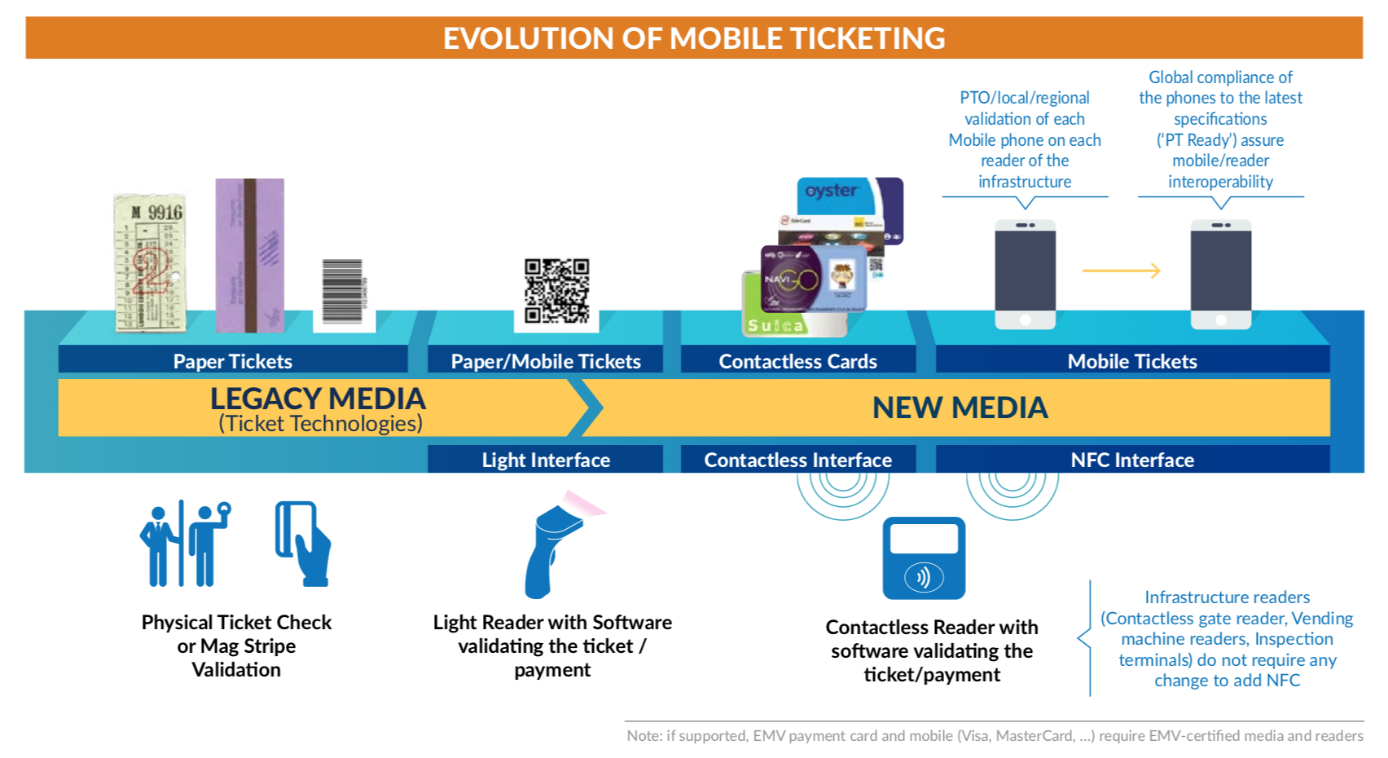
\includegraphics[width=0.9\linewidth]{image/smart_cards} \caption{The evolution of mobile ticketing (NFC Forum, 2016)}\label{fig:unnamed-chunk-31}
\end{figure}

Furthermore, current research addresses the issues of big data and how collected data through contactless smart cards can be best analysed (see Kurauchi \& Schmöcker, 2017). Recent studies investigated a prototype of the BI/BO (be in/be out) system, working in the public transport system in Lodz, Poland. The Passenger BIBO and automation of the CICO (check-in/check-out) give rise to a new approach to an integrated passenger identification model by applying machine learning technologies and using Internet of Things (IoT), through beacons and smartphones. It enables wireless connection with the use of bluetooth and automatic detection of passengers (Hasimi et al., 2021; Mastalerz et al, 2020). Bieler et al.~(2022) explored solutions for automated fare collection in public transportation and found significant positive impacts on consumer experiences and reduction of pollutant emissions in urban transportation due to a more seamless and efficient fare collection systems.

\hypertarget{current-state-of-art-in-practice-26}{%
\subsection*{Current state of art in practice}\label{current-state-of-art-in-practice-26}}
\addcontentsline{toc}{subsection}{Current state of art in practice}

Many countries, regions or cities, have smart card ticketing systems in use, like the whole of Netherlands, Helsinki Region, Minsk, Berlin, Auckland, Sydney and many more (see Wikipedia contributors, 2021). The systems itself differ and depend on the local ticketing and fare systems. While London, for instance, is using an access control system, Helsinki's system is trust based. Furthermore, a distinction can be made between pre-paid (debit) and post-paid (credit) systems (Kurauchi \& Schmöcker, 2017). Current CICO (check in/check out) systems are available as the Oyster Card in London, the EZ-Link Card in Singapur, OV-chipkaart in Amsterdam, LisboaViva Card in Lisbon, go card in Brisbane, Octopus in Hongkong, AltoAdige Pass in SüdTyrol (Eilmes et al., 2014), while BIBO systems (be in/be out) have only been tested, but not been implemented on a wide range (N.N., 2009). Furthermore, Biometric Ticketing (e.g.~by facial recognition) is tested in various countries (China: Shenzhen Metro, Japan: Osaka Metro, London: Eurostar) and by Amazon (Singh, 2021).

\hypertarget{relevant-initiatives-in-austria-26}{%
\subsection*{Relevant initiatives in Austria}\label{relevant-initiatives-in-austria-26}}
\addcontentsline{toc}{subsection}{Relevant initiatives in Austria}

\begin{itemize}
\tightlist
\item
  \href{https://taikai.network/en/wiener-linien/challenges/tickethon}{taikai.network}
\item
  \href{https://www.variuscard.com/}{variuscard}
\item
  \href{https://www.austriacard.com/}{austriacard}
\end{itemize}

\hypertarget{impacts-with-respect-to-sustainable-development-goals-sdgs-26}{%
\subsection*{Impacts with respect to Sustainable Development Goals (SDGs)}\label{impacts-with-respect-to-sustainable-development-goals-sdgs-26}}
\addcontentsline{toc}{subsection}{Impacts with respect to Sustainable Development Goals (SDGs)}

\begin{longtable}[]{@{}
  >{\centering\arraybackslash}p{(\columnwidth - 8\tabcolsep) * \real{0.2029}}
  >{\centering\arraybackslash}p{(\columnwidth - 8\tabcolsep) * \real{0.1884}}
  >{\centering\arraybackslash}p{(\columnwidth - 8\tabcolsep) * \real{0.2029}}
  >{\centering\arraybackslash}p{(\columnwidth - 8\tabcolsep) * \real{0.2029}}
  >{\centering\arraybackslash}p{(\columnwidth - 8\tabcolsep) * \real{0.2029}}@{}}
\toprule()
\begin{minipage}[b]{\linewidth}\centering
Impact level
\end{minipage} & \begin{minipage}[b]{\linewidth}\centering
Indicator
\end{minipage} & \begin{minipage}[b]{\linewidth}\centering
Impact direction
\end{minipage} & \begin{minipage}[b]{\linewidth}\centering
Goal description and number
\end{minipage} & \begin{minipage}[b]{\linewidth}\centering
Source
\end{minipage} \\
\midrule()
\endhead
Individual & Personal, travel expenditure reduced & \textbf{+} & Sustainable economic development (\emph{8,11}) & Turner \& Wilson, 2010 \\
Individual & Access to digitalised transport & \textbf{+} & Innovation \& Infrastructure (\emph{9}) & Turner \& Wilson, 2010 \\
Systemic & Public transport capacity increases & \textbf{+} & Sustainable economic development (\emph{8,11}) & Turner \& Wilson, 2010 \\
Systemic & Facilitates integration of the fare systems of several operators within a city & \textbf{+} & Partnership \& collaborations (\emph{17}) & Kurauchi \& Schmoecker, 2017 \\
\bottomrule()
\end{longtable}

\hypertarget{technology-and-societal-readiness-level-26}{%
\subsection*{Technology and societal readiness level}\label{technology-and-societal-readiness-level-26}}
\addcontentsline{toc}{subsection}{Technology and societal readiness level}

\begin{longtable}[]{@{}cc@{}}
\toprule()
TRL & SRL \\
\midrule()
\endhead
7-9 & 7-9 \\
\bottomrule()
\end{longtable}

\hypertarget{open-questions-24}{%
\subsection*{Open questions}\label{open-questions-24}}
\addcontentsline{toc}{subsection}{Open questions}

\begin{enumerate}
\def\labelenumi{\arabic{enumi}.}
\tightlist
\item
  How can the large amount of provided data be best used?
\item
  What advantages and disadvantages would an implementation in the main cities of Austria have?
\end{enumerate}

\hypertarget{further-links-22}{%
\subsection*{Further links}\label{further-links-22}}
\addcontentsline{toc}{subsection}{Further links}

\begin{itemize}
\tightlist
\item
  \href{https://www.itso.org.uk/}{itso}
\end{itemize}

\hypertarget{references-26}{%
\subsection*{References}\label{references-26}}
\addcontentsline{toc}{subsection}{References}

\begin{itemize}
\tightlist
\item
  Bieler, M., Skretting, A., Büdinger, P., Gronli, T.-M. 2022. Survey of Automated Fare Collection Solutions in Public Transportation. IEEE Transactions on Intelligent Transport Systems. Doi: 10.1109/TITS.2022.3161606
\item
  Eilmes, B., Zietz, A., Szombathely, M., Quast, F., Blanckmeister, C., Schmiede, A. 2014. CICO-, CIBO und BIBO-basierte ÖPNV-Vertriebssysteme in Ballungsräumen weltweit (Markterkundung). VRR: Verkehrsverbung Rhei-Ruhr AöR. Available at: \url{https://docplayer.org/storage/18/893383/1658415222/cRaJu2SV6CLCYsoiVAwLEQ/893383.pdf} {[}Accessed: 21 July 2022{]}
\item
  Hasimi, L., Poniszewska-Maranda, A., Krym, T. 2021. Smart City Concept Using BI/BO Model for the Ticket System in Urban Transport. IEEE Transactions on Intelligent Transport Systems. \url{https://doi.org/10.23919/SoftCOM52868.2021.9559116}
\item
  Kurauchi, F., \& Schmöcker, J. D. (Eds.). (2017). Public transport planning with smart card data. CRC Press.
\item
  Mastalerz, M., Malinowski, A., Kwiatkowski, S., Sniegula, A., Wieczorek, B. 2020. Passenger BIBO detection with IoT support and machine learning techniques for intelligent transport systems. Procedia Computer Science. 176. 3780-3793. \url{https://doi.org/10.1016/j.procs.2020.09.009}
\item
  Mezghani, M. (2008). Study on electronic ticketing in public transport. European Metropolitan Transport Authorities (EMTA), 56, 38.
\item
  NFC Forum. (2016). NFC-enabled e-Ticketing in Public Transport: Clearing the Route to Interoperability. December. \url{https://nfc-forum.org/wp-content/uploads/2016/12/NFC_enabled_eTicketing_in_Public_Transport_White_Paper.pdf}
\item
  N.N. (2009). Be-In-Be-Out Payment Systems for Public Transport: Final Report. Department for Transport (London). Available at: \url{https://manualzz.com/download/2984265} {[}Accessed: 29 July 2022{]}
\item
  Singh, J. (2021). Payment apps, CiBo, and biometricts: what's next for mobile ticketing? Intelligent Transport. Available at: \url{https://www.intelligenttransport.com/transport-articles/114876/future-of-mobile-ticketing/} {[}Accessed: 20 July 2022{]}
\item
  ÖBB. Ihr Weg zum Ticket. Available at: \url{https://www.oebb.at/de/tickets-kundenkarten/weg-zum-ticket} {[}Accessed: 13 January 2021{]}
\item
  Turner, M., \& Wilson, R. (2010). Smart and integrated ticketing in the UK: Piecing together the jigsaw. Computer Law \& Security Review, 26(2), 170-177.
\item
  Wels Linien. Tarife. Available at: \url{https://www.welslinien.at/tarife/} {[}Accessed: 13 January 2021{]}
\item
  Wiener Linien. (2021a). Der richtige Fahrschein,
  der passende Tarif. Available at: \url{https://www.wienerlinien.at/eportal3/ep/channelView.do/pageTypeId/66526/channelId/-46648} {[}Accessed: 13 January 2021{]}
\item
  Wiener Linien. (2021b). Digital-Wettbewerb ``Vienna Tickethon'' gestartet. Available at: \url{https://www.wienerlinien.at/eportal3/ep/contentView.do/pageTypeId/66526/programId/74577/contentTypeId/1001/channelId/-47186/contentId/5002360\#}:\textasciitilde:text=Im\%20Rahmen\%20eines\%20internationalen\%20Hackathon,Wettbewerb\%20l\%C3\%A4uft\%20bis\%20Anfang\%20M\%C3\%A4rz {[}Accessed: 13 January 2021{]}
\item
  Wikipedia contributors. (2021, January 8). List of smart cards. In Wikipedia, The Free Encyclopedia. Available at: \url{https://en.wikipedia.org/w/index.php?title=List_of_smart_cards\&oldid=999040130} {[}Accessed: 13 January 2021{]}
\end{itemize}

\hypertarget{special_needs}{%
\section{Information and assistance for people with special needs}\label{special_needs}}

\textbf{Updated: 6th August 2022}

\hypertarget{synonyms-23}{%
\subsection*{Synonyms}\label{synonyms-23}}
\addcontentsline{toc}{subsection}{Synonyms}

\emph{Assistive technology}

\hypertarget{definition-27}{%
\subsection*{Definition}\label{definition-27}}
\addcontentsline{toc}{subsection}{Definition}

Vehmas (2010: 92) defines that having a special need \emph{``\ldots implies that an individual has the kind of characteristics that it is unlikely, or at least uncertain, whether he or she would achieve the aim that defines the need in question without special instruction, procedures that are out of ordinary.''} Special needs can therefore mean a mobility limitation due to age or any type of disability.

Furthermore, \emph{``Assistive technology refers to any system, services, appliances or devices that could be used to help disabled people with their daily life by removing some barriers to activities.''} (Low et al., 2020).

Because the types of disabilities are diverse and so are the specific needs, Low et al.~(2020) argue that more specific measures should be taken to meet the particular needs of specific disabilities rather than generalizing the types of assistive devices available. The requirements regarding traffic systems for people with special needs can be divided into \emph{(1)} visual impairment, \emph{(2)} hearing impairment, \emph{(3)} mobility impairment, and \emph{(4)} mental impairment. While for some people with special needs only one may be applicable, the elderly people might depend upon more than one or even all.

Low et al.~(2020) argue, that especially people with visual impairment (VIP) are dependent on public transport, because they cannot drive vehicles themselves, which leads to a restriction of freedom of movement. The same applies to many people with limited mobility who are excluded from active participation in motorized individual transport. Limited access to travel information is often a barrier to independent travel and other daily activities for people with special needs. When using public transportation, the choice of route is influenced by the reliability and availability of information, as well as convenience and comfort. However simply gathering this information before a trip can often be a problem for VIPs, as a lot of information is printed. However, the current trend towards online materials is helping. Due to physical and mental conditions, especially old or disabled people might need some extra information, for example, many older people cannot stand for long, are sensitive to weather conditions, cannot do things quickly or cannot walk long distances (Hounsell et al., 2016). A lack of usable information can add a negative aspect to the overall experience and actually prevent a trip.

In addition, Low et al.~(2020) argue, that bus riding poses several challenges for VIPs, such as finding the right bus, which is especially problematic when multiple bus stops are at the same station. The mix of fleets used makes it difficult for VIPs to identify the characteristics of a bus. Furthermore, it is often difficult for VIPs to locate the boarding point for buses. Regarding trains, the gap between the train and the platform can be a barrier. An important part of public transport are audio announcements, which serve as a source of information for VIPs. If these systems fail, the journey is perceived as particularly stressful.

To overcome barriers at the ticket buying, the implementation of contactless card systems (see \protect\hyperlink{contactless_cards}{Contactless public transport cards section}) or free passes for disabled people can help (Low et al., 2020).

\hypertarget{key-stakeholders-27}{%
\subsection*{Key stakeholders}\label{key-stakeholders-27}}
\addcontentsline{toc}{subsection}{Key stakeholders}

\begin{itemize}
\tightlist
\item
  \textbf{Affected}: People with special needs, elderly population, care takers
\item
  \textbf{Responsible}: Transport service providers and public transport operators, MaaS operators and integrators, IT system providers, city councils, local, regional and national authorities, public transport associations, industry suppliers, Association for the Blind, Association for the Disabled
\end{itemize}

\hypertarget{current-state-of-art-in-research-27}{%
\subsection*{Current state of art in research}\label{current-state-of-art-in-research-27}}
\addcontentsline{toc}{subsection}{Current state of art in research}

The study by Low et al.~(2020) reflects, among other things, VIPs' desire to be independent in planning their trips by using online resources rather than seeking help from others. This shows the importance of having appropriate online tools for VIPs. Interviewees mentioned that they need to use many different sources and apps to plan a single trip, which in turn causes a lot of stress and decreases the propensity to the use of public transport. In addition, VIPs were found to lack access to current policies and information on available assistance. Furthermore, it was pointed out, that a similar interior design of buses would be extremely helpful for VIP and increase safety.

Goldberg et al.~(2018) looked into the needs of VIPs for orientation, navigation and mobility. Based on their findings, they propose \emph{``an integrated cyber-physical system (CPS) framework with `Agents' and `Smart Environments' to address VIP's ONM needs in urban settings.''} Fusco \& Coughlan (2020) described \emph{``a computer vision approach to indoor localization that runs as a real-time app on a conventional smart-phone, which is intended to support a full-featured wayfinding app in the future that will include turn-by-turn directions.''} One advantage of this approach is that no new infrastructure is needed, just a working smartphone with a built-in camera.

Hounsell et al.~(2016) addressed information needs of older people particularly using public transport. Among other things, they found that elderly people \emph{``may need larger font displays and primary data only, while mobility impaired people may need information on walking distances and the existence of gradient, steps, seats, etc.''} By reviewing international cases of open data implementation, they found examples of authorities initiating the market by running competitions to develop apps for targeted groups such as older or disabled people.

Kassens-Noor et al.~(2021) studied the effect of \protect\hyperlink{connected}{autonomous vehicles} for people with special needs and found, that along with the potential to increase mobility for these populations they are still not considered in most research. In their survey, they found significant differences among different special needs groups in their willingness to use APT (autonomous public transport). The results, therefore, suggest that people with special needs perceive AVs primarily negatively and need further attention in future research. Other studies researched the adoption of assistive technology among disabled people and show that there is a variability of technology adoption depending on the type of disability (König et al., 2022) but also that the main drivers of the use of assistive technology are the advancement of living standards and enhancement of users' performance (Salim et al., 2022). Furthermore, a recent study addressed the problem of accessible maps for indoor and outdoor mobility. It proposed making information about buildings available and creating tactile indoor maps and accessible navigation apps which are also adaptable to the users' needs (Loitsch et al., 2022).

\hypertarget{current-state-of-art-in-practice-27}{%
\subsection*{Current state of art in practice}\label{current-state-of-art-in-practice-27}}
\addcontentsline{toc}{subsection}{Current state of art in practice}

One of the common assistive tools available to VIP are mobility tools, in particular a long cane or a guide dog. GPS is used as an assistive technology for VIP for orientation purposes and as a navigation aid. It can also be integrated into other devices to help VIP with orientation, such as a GPS-based voice alarm system that alerts VIP to nearby obstacles (Low et al., 2020). Additionally, a variety of initiatives and technologies to promote the inclusion of people with special needs creating software that help to give voice to people with communication difficulties (The Open Voice Factory) or researching on smartphone tools to integrate people with intellectual disabilities (Disability Innovation Institute) (Gervais, 2022). \emph{BlindSquare} is one of the most popular GPS apps in the world for blind and visually impaired people. It describes the surroundings, warns about street intersections and important points as one moves along. Used in conjunction with external free navigation apps, \emph{BlindSquare} provides almost all the information blind and visually impaired people need to be independent on the road. \emph{BlindSquare} determines the location using the smartphone's GPS capabilities and retrieves information about the surrounding area on Foursquare and Open Street Map. Thanks to its unique algorithms, it determines the most relevant information and states it clearly in an artificial voice (BlindSquare., n.d.). A similar app is \emph{Seeing Assistant Move}, which is based on Google Maps and also works offline and with voice control (Transition Technologies S.A., n.d.). Using public transport audio announcements plays a crucial role in helping VIP to be prepared to alight from the vehicle (Low et al., 2020).

Induction hearing systems or induction hearing loops are used to provide people with hearing problems with auditory information. The principle is based on special cables, the so-called induction loop, which is operated by an induction amplifier that converts the signals coming from the microphone and feeds them into the loop as a current. This current, in turn, creates a weak magnetic field in the coil in the room, which pulses in rhythm with the speech. This weak magnetic field is picked up by the hearing aid's T-coil, similar to an antenna, and converted back into audible sound vibrations. Almost no background noise is transmitted and the desired information can thus be heard without interference, almost in HIFI quality (Sturma, 2011).

To ensure accessibility for people with limited mobility in buses, more and more cities are focusing on the use of low-floor vehicles that can be lowered further hydraulically if required. The low entrance height makes boarding and alighting much easier, especially for older people and passengers with baby carriages or wheelchair users. Tramway equipment is also constantly being improved. Modern cars have more space for passengers with wheelchairs or baby carriages and a retractable ramp to bridge the already minimized gap between the platform edge and the vehicle (Wiener Linien, n.d.). As in Vienna, for example, real-time displays at stations can use a wheelchair symbol to indicate whether the expected public transport vehicles are barrier-free.

Finally, for example in Singaporean buses were introduced amenities for the convenience of pregnant, elderly and young passengers in the form of designated priority seats, low floors along the entire bus and low steps at the entrance and exit to facilitate individuals with limited mobility to board the bus quickly as well as move along the bus more easily (Smrt.com.sg, 2021).

\hypertarget{relevant-initiatives-in-austria-27}{%
\subsection*{Relevant initiatives in Austria}\label{relevant-initiatives-in-austria-27}}
\addcontentsline{toc}{subsection}{Relevant initiatives in Austria}

\begin{itemize}
\tightlist
\item
  \href{https://www.oebb.at/de/reiseplanung-services/barrierefrei-reisen}{oebb.at}
\item
  \href{https://www.wienerlinien.at/web/wiener-linien/neue-bim-und-bus-haltestellen-f\%C3\%BCr-wien}{wienerlinien.at}
\item
  \href{https://www.induktionsschleife.at/}{induktionsschleife.at}
\end{itemize}

\hypertarget{impacts-with-respect-to-sustainable-development-goals-sdgs-27}{%
\subsection*{Impacts with respect to Sustainable Development Goals (SDGs)}\label{impacts-with-respect-to-sustainable-development-goals-sdgs-27}}
\addcontentsline{toc}{subsection}{Impacts with respect to Sustainable Development Goals (SDGs)}

\begin{longtable}[]{@{}
  >{\centering\arraybackslash}p{(\columnwidth - 8\tabcolsep) * \real{0.2029}}
  >{\centering\arraybackslash}p{(\columnwidth - 8\tabcolsep) * \real{0.1884}}
  >{\centering\arraybackslash}p{(\columnwidth - 8\tabcolsep) * \real{0.2029}}
  >{\centering\arraybackslash}p{(\columnwidth - 8\tabcolsep) * \real{0.2029}}
  >{\centering\arraybackslash}p{(\columnwidth - 8\tabcolsep) * \real{0.2029}}@{}}
\toprule()
\begin{minipage}[b]{\linewidth}\centering
Impact level
\end{minipage} & \begin{minipage}[b]{\linewidth}\centering
Indicator
\end{minipage} & \begin{minipage}[b]{\linewidth}\centering
Impact direction
\end{minipage} & \begin{minipage}[b]{\linewidth}\centering
Goal description and number
\end{minipage} & \begin{minipage}[b]{\linewidth}\centering
Source
\end{minipage} \\
\midrule()
\endhead
Individual & Safe access to public transport for people with special needs & \textbf{+} & Health \& Wellbeing (\emph{3}) & Low et al.~(2020) \\
Individual & Equal freedom of movement for people with special needs & \textbf{+} & Equality (\emph{5,10}) & Low et al.~(2020) \\
Individual & Improved access to public transport & \textbf{+} & Environmental sustainability (\emph{7,12-13,15}) & Low et al.~(2020) \\
Systemic & Increase in innovative apps developed for targeted groups; use of open data & \textbf{+} & Innovation \& Infrastructure (\emph{9}) & Hounsell et al.~(2016) \\
\bottomrule()
\end{longtable}

\hypertarget{technology-and-societal-readiness-level-27}{%
\subsection*{Technology and societal readiness level}\label{technology-and-societal-readiness-level-27}}
\addcontentsline{toc}{subsection}{Technology and societal readiness level}

\begin{longtable}[]{@{}cc@{}}
\toprule()
TRL & SRL \\
\midrule()
\endhead
3-7 & 3-7 \\
\bottomrule()
\end{longtable}

\hypertarget{open-questions-25}{%
\subsection*{Open questions}\label{open-questions-25}}
\addcontentsline{toc}{subsection}{Open questions}

\begin{enumerate}
\def\labelenumi{\arabic{enumi}.}
\tightlist
\item
  How could real-time information be better available for visually impaired people?
\item
  How could audio announcements be improved?
\item
  How to improve staff assistance?
\item
  How could smart technologies become more accessible to older people?
\end{enumerate}

\hypertarget{further-links-23}{%
\subsection*{Further links}\label{further-links-23}}
\addcontentsline{toc}{subsection}{Further links}

\begin{itemize}
\tightlist
\item
  \href{https://www.blindsquare.com/de/about/}{blindsquare.com}
\item
  \href{http://seeingassistant.tt.com.pl/move/}{seeingassistant.tt.com.pl}
\item
  \href{https://www.induktionsschleife.at/anwendungen/}{induktionsschleife.at}
\item
  \href{https://www.oebb.at/de/reiseplanung-services/barrierefrei-reisen}{oebb.at}
\item
  \href{https://www.wienerlinien.at/eportal3/ep/contentView.do?pageTypeId=66526\&channelId=-47186\&programId=74577\&contentId=5002349\&contentTypeId=1001}{wienerlinien.at}
\item
  \href{https://www.oesb-dachverband.at/}{oesb-dachverband.at}
\item
  \href{https://www.blindenverband.at/}{blindenverband.at}
\item
  \href{https://avencod.fr/quisommenous}{Avencod}
\end{itemize}

\hypertarget{references-27}{%
\subsection*{References}\label{references-27}}
\addcontentsline{toc}{subsection}{References}

\begin{itemize}
\tightlist
\item
  BlindSquare. (n.d.). What is BlindSquare? Available at: March 4, 2021, from \url{https://www.blindsquare.com/about/} {[}Accessed: 4 March 2021{]}
\item
  Fusco, G., \& Coughlan, J. M. (2020, April). Indoor localization for visually impaired travelers using computer vision on a smartphone. In Proceedings of the 17th International Web for All Conference (pp.~1-11).
\item
  Gervais, Z. (2021). Disability as an Innovation Driver for the Smart City. Inclusive City Maker. Available at: \url{https://www.inclusivecitymaker.com/disability-innovation-driver-smart-city/} {[}Accessed: 1 August 2022{]}
\item
  Goldberg, M., Zhu, Z., \& Zhang, Z. (2018). How do we aid visually impaired people safely manage unfamiliar environments?.
\item
  Hounsell, N. B., Shrestha, B. P., McDonald, M., \& Wong, A. (2016). Open data and the needs of older people for public transport information. Transportation research procedia, 14, 4334-4343.
\item
  Kassens-Noor, E., Cai M., Kotval-Karmchandani, Z., Decaminda, T. (2021). Autonomous vehicles and mobility for people with special needs. Transportation Research Part A. 150, 385-397. \url{https://doi.org/10.1016/j.tra.2021.06.014}
\item
  König, A., Alciauskaite, L., Hatzakis, T. (2022). The Impact of Subjective Technology Adaptivity on the Willingness of Persons with Disabilities to Use Emerging Assistive Technologies: A European Persepective. International Conference on Computers Helping People with Special Needs. ICCHP-AAATE 2022, pp 207-214. Available at: \url{https://link.springer.com/chapter/10.1007/978-3-031-08648-9_24} {[}Accessed: 31 July 2022{]}
\item
  Loitsch, C., Müller, K., Weber, G., Petrie, H., Stiefelhagen, R. (2022). Digital Solutions for Inclusive Mobility: Solutions and Accessible Maps for Indoor and Outdoor Mobility. International Conference on Computers Helping People with Special Needs. 95-101. DOI: 10.1007/978-3-031-08648-9\_12
\item
  Low, W. Y., Cao, M., De Vos, J., \& Hickman, R. (2020). The journey experience of visually impaired people on public transport in London. Transport Policy, 97, 137-148.
\item
  Smrt.com.sg. (2021). Accessibility. Smrt.com.sg. Available at: \url{https://www.smrt.com.sg/Journey-with-Us/SMRT-Buses/Accessibility} {[}Accessed: 12 March 2021{]}.
\item
  Sturma, A. (2011). Höranlagen. \url{https://www.oessh.or.at/hoerspuren/hoeranlagen}
\item
  Transition Technologies S.A. (n.d.). Seeing Assistant Move - Features. Available at: \url{http://seeingassistant.tt.com.pl/move/} {[}Accessed: 4 March 2021{]}
\item
  Vehmas, S. (2010). Special needs: a philosophical analysis. International journal of inclusive education, 14(1), 87-96.
\item
  Wiener Linien. (n.d.). Barrierefreiheit bei den Wiener Linien - Wiener Linien. Available at: \url{https://www.wienerlinien.at/web/wiener-linien/barrierefreiheit} {[}Accessed: 16 March 2021{]}
\end{itemize}

\hypertarget{mobility_hubs}{%
\section{Mobility hubs}\label{mobility_hubs}}

\textbf{Updated: 6th August 2022}

\hypertarget{synonyms-24}{%
\subsection*{Synonyms}\label{synonyms-24}}
\addcontentsline{toc}{subsection}{Synonyms}

\emph{Mobility station or point, mobihub, (public) ride point, smart station, sharing zone, transportation center, public transit or transport hub, transport interchange, ride port, share point, intermodal hubs}

\hypertarget{definition-28}{%
\subsection*{Definition}\label{definition-28}}
\addcontentsline{toc}{subsection}{Definition}

There are many different definitions of mobility hubs. In general, mobility hubs are places to change transport mode. However, they can also be much more than that and are essential for the functioning of Mobility as a Service (See \protect\hyperlink{maas}{MaaS}). Mobility hubs are expected to be convenient and safe for switching modes, but they could also close supply gaps, enhance traveller experience and the quality of life in a certain area (Clemens, 2020). Airports, train and subway stations usually include car park and car rental, bus stops and taxi stands as well as restaurants, shops, hotels or even conference centres, which benefit from passing trade and goods accessibility. They represent so-called ``\emph{naturally}'' grown mega hubs (Clemens, 2020). In addition, municipalities around the world are systematically planning and implementing further mobility hubs that vary in size - from a small bus stop with an attached bike sharing station to a mega hub as described above. They are supposed to improve intermodal mobility and bring socio-economic benefits (Clemens, 2020). Specific names and strong visual branding are designed to help passengers recognize them quickly.

Mobility as a Service or Mobility on Demand concepts are designed to make it possible to not own a car and still be mobile. Mobility hubs should offer the greatest possible variation of means of transport for individual route chains and thus, ensure that car journeys are not all replaced one-to-one by car sharing journeys, but that the transport routes are covered as sustainably as possible (Clemens, 2020). Since each additional transfer during a trip creates a barrier and tempts people to use private motorized transport instead, the goal of mobility hubs is to provide these transfers with a benefit and to ensure that the transfer runs smoothly. Examples include allowing people to work or relax, pick up a package, meet friends, or do necessary shopping during their commute home (Clemens, 2020). Mobility hubs could also be combined with quarter logistics hubs (See \protect\hyperlink{urban_delivery}{Urban deliveries}) (Herrmann, n.d.).

\hypertarget{key-stakeholders-28}{%
\subsection*{Key stakeholders}\label{key-stakeholders-28}}
\addcontentsline{toc}{subsection}{Key stakeholders}

\begin{itemize}
\tightlist
\item
  \textbf{Affected}: Public and private transport users, Commuters\\
\item
  \textbf{Responsible}: City administration, Public transport operators, Mobility service providers, District authorities, Private companies, Shared mobility providers
\end{itemize}

\hypertarget{current-state-of-art-in-research-28}{%
\subsection*{Current state of art in research}\label{current-state-of-art-in-research-28}}
\addcontentsline{toc}{subsection}{Current state of art in research}

Bell (2019) has analysed the user requirements of mobility hubs. He argues that mobility hubs or intermodal hubs differ depending on the area in which they are implemented, e.g.~rural or urban areas, and that success and sustainability strongly depend on the particular design. An overview of his general conclusion is shown in Figure 7.2.

\begin{figure}
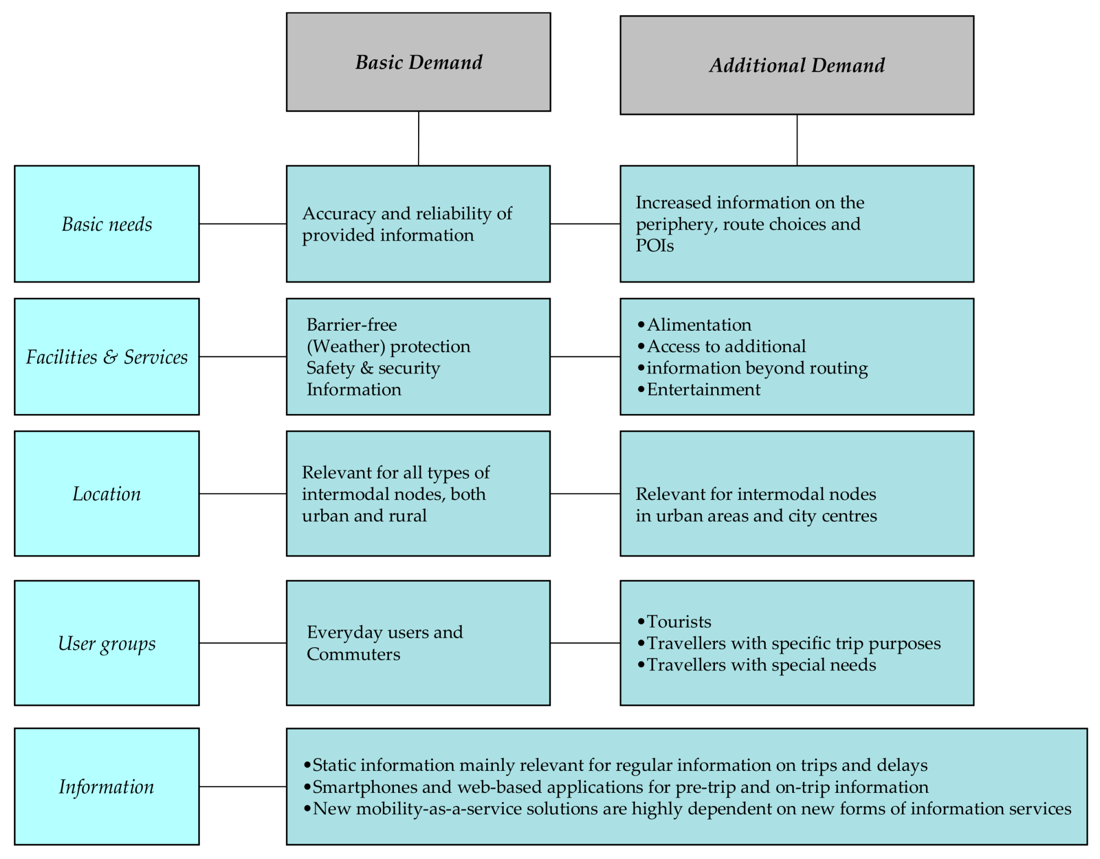
\includegraphics[width=0.65\linewidth]{image/mobility_hubs} \caption{: User requirements at public transport stops (Bell, 2019)}\label{fig:unnamed-chunk-32}
\end{figure}

Based on research conducted in American cities, Hochmair (2015) argues, that it is recommended to ensure improved cycling infrastructure, such as bike-sharing stations, within a 1-mile radius for bus-only stations and within 2 miles for train stations.

Tran \& Draeger (2021) have presented a new evaluation framework and algorithm to locate and assess the sustainability and equity impacts of nodes in cities. Investment strategies for nodes are evaluated based on \emph{(1)} current mode split, \emph{(2)} high transit capacity, and \emph{(3)} multimodal services. From an equity perspective, high transit capacity and multimodal node strategies include more low-income areas than the current mode split, which primarily covers middle-income areas. The results of the study show how municipalities can strategically invest in public transit and multimodal options to increase frequency, quality and overall mobility for low- and moderate-income households and improve access to key facilities for more vulnerable citizens. Municipalities can use the assessment framework to explore alternative transport investment scenarios. This should make it possible to spatially locate urban hubs to meet future transport demand, increase the uptake of multimodal services and improve equal access for all citizens. A methodology by Blad (2021), to determine the potential of areas for regional mobility hubs was conducted and tested in the city of Rotterdam. It consists of five criteria (potential demand, costs, generalized travel costs, link to surroundings and impact) which are measured by nine attributes and shows suitability to tackle the location potential determination problem.

Franken (2021) investigated the potential of mobility hubs to reduce car use and car ownership and also how these are influenced by the characteristics of the car owner, the characteristics of the trip and the characteristics of the car owner's living environment. His results showed that the operating costs of shared mobility services and walking distances to mobility hubs are important determinants of the use of shared mobility services, with higher sensitivity to operating costs for the shared e-car than for shared e-mopeds and e-bikes. Furthermore, he found that the density of mobility hubs in a residential area has a strong impact on reducing car use and car ownership. This matches with the fact that the impact of mobility hubs on car use and car ownership was highest in the city center, followed by a suburban area and lowest in a rural area.

In 2018, MA 18 - Urban Development and Planning and MA 21 - District Planning and Land Use of the City of Vienna published a guideline for the implementation of mobility stations in urban development areas (Stadt Wien - Stadtentwicklung und Stadtplanung (MA 18) \& Stadtteilplanung und Flächennutzung (MA 21), 2018). On behalf of the German Federal Ministry for the Environment, Nature Conservation and Nuclear Safety (BMU), also the German Institute of Urban Affairs (Deutsches Institut für Urbanistik) published a report in 2019 on the findings and experiences on mobility stations in municipal practice (Stein \& Bauer, 2019).

ETH Zurich (Wicki et al., 2022) conducted a survey in three cities that aimed to identify social requirements. They found that the most important feature of mobility hub is the offer of different mobility systems, while the second most important is its contribution to the open space (as a part of identity in a social setting). Nonetheless, there is a general lack of knowledge and awareness for micro mobility (especially e-scooters) and its last mile coverage was mostly highly criticised. Missing social acceptance can be seen as a main contributor to slower adoption of mobility hubs. Researchers, therefore, suggest to identify the needs of users and raise awareness and knowledge in this area.

\hypertarget{current-state-of-art-in-practice-28}{%
\subsection*{Current state of art in practice}\label{current-state-of-art-in-practice-28}}
\addcontentsline{toc}{subsection}{Current state of art in practice}

In order to promote both the health and quality of life of citizens, while improving sustainability and accessibility in transportation within cities, six partner cities from five different countries have committed to establish so-called e-Mobility Hubs, in short eHUBS. eHUBS are on-street locations that bring together e-bikes, e-cargo bikes, e-scooters and/or e-cars, offering users a wide range of options to experiment with and use in different situations. These dedicated on-street locations, where citizens can choose from a variety of sustainable electric transportation options for shared use, are intended to provide a true alternative to private car use by offering opportunities to increase shared and electric mobility in a truly innovative way. Hubs can vary in size (minimalist, light, medium, large), type of location, and type of service. They can be small and located in residential areas, with only one or two parking spaces, or larger and positioned near train stations and major public transit hubs, but ultimately the key is that they should always be where supply and demand meet. The knowledge and experience gained will, then help other cities and regions get close and consistently tackle air pollution, congestion and CO\textsubscript{2} emissions, and create a growing market for commercial e-mobility providers (Interreg North-West Europe (NWE), 2019).

In Vienna, there are already 8 so-called ``\emph{WienMobil Stations}'' operated by Wiener Linien, which combine access to public transport with various services and sharing offers. They vary by station, but can include bike sharing, scooter sharing, moped sharing, car sharing, bike service station, cab, e-charging station, bike storage boxes, cargo bikes (Wiener Linien, 2021).

Beyond, in the cities of Graz and Linz and the Styrian Central Region, mobility hubs called ``\emph{tim}'' have been implemented. They combine public transport stations with (e-)car sharing, call-collection taxis, bicycle parking facilities and rentable cargo bikes (see \href{https://www.tim-oesterreich.at}{tim-oesterreich}). Additionally, the small city of Weiz (close to Graz) implemented smart mobility and two new mobility hubs in 2022 including e-car sharing, WASTI (a called and shared cab) and WeizBike (Interreg Central Europe (CE), 2022).

In the Netherlands, too, there are already several Mobility hubs of various types. One example is the hub P+R Gieten, which is located at the transport hub Gieten and has a fast connection to Groningen, Veendam, Stadskanaal, Emmen and Assen via the N33 and N34. The hub allows a transfer between Qliners and regional buses and is the main bus stop for the villages of Gieten and Eext. At this hub there are two free parking facilities, a spacious covered bike shed, lockers and a kiosk, a wheelchair accessible toilet and outdoor fitness equipment. Also, there are two types of bicycle lockers. Boxes that can be opened with a key and boxes that can be reserved and opened with an app (Reisviahub.nl, n.d.).

\hypertarget{relevant-initiatives-in-austria-28}{%
\subsection*{Relevant initiatives in Austria}\label{relevant-initiatives-in-austria-28}}
\addcontentsline{toc}{subsection}{Relevant initiatives in Austria}

\begin{itemize}
\tightlist
\item
  \href{https://www.wienerlinien.at/web/wiener-linien/wienmobil-stationen}{wienmobil-stationen}
\item
  \href{https://www.tim-oesterreich.at}{tim-oesterreich}
\item
  \href{https://www.wien.gv.at/stadtentwicklung/studien/pdf/b008521.pdf}{wien.gv.at}
\item
  \href{https://www.austriatech.at/assets/Uploads/Publikationen/PDF-Dateien/03251beacc/Mobility-Explored_Sharing-Mobility-032019.pdf}{AustriaTech}
\end{itemize}

\hypertarget{impacts-with-respect-to-sustainable-development-goals-sdgs-28}{%
\subsection*{Impacts with respect to Sustainable Development Goals (SDGs)}\label{impacts-with-respect-to-sustainable-development-goals-sdgs-28}}
\addcontentsline{toc}{subsection}{Impacts with respect to Sustainable Development Goals (SDGs)}

\begin{longtable}[]{@{}
  >{\centering\arraybackslash}p{(\columnwidth - 8\tabcolsep) * \real{0.2029}}
  >{\centering\arraybackslash}p{(\columnwidth - 8\tabcolsep) * \real{0.1884}}
  >{\centering\arraybackslash}p{(\columnwidth - 8\tabcolsep) * \real{0.2029}}
  >{\centering\arraybackslash}p{(\columnwidth - 8\tabcolsep) * \real{0.2029}}
  >{\centering\arraybackslash}p{(\columnwidth - 8\tabcolsep) * \real{0.2029}}@{}}
\toprule()
\begin{minipage}[b]{\linewidth}\centering
Impact level
\end{minipage} & \begin{minipage}[b]{\linewidth}\centering
Indicator
\end{minipage} & \begin{minipage}[b]{\linewidth}\centering
Impact direction
\end{minipage} & \begin{minipage}[b]{\linewidth}\centering
Goal description and number
\end{minipage} & \begin{minipage}[b]{\linewidth}\centering
Source
\end{minipage} \\
\midrule()
\endhead
Individual & Improved accessibility & \textbf{+} & Equality (\emph{5,10}) & Miramontes et al., (2017) \\
Individual & Increased multimodal trips & \textbf{+} & Sustainable economic development (\emph{8,11}) & Miramontes et al., (2017) \\
Systemic & Reduced car use and car ownership & \textbf{+} & Environmental sustainability (\emph{7,12-13,15}) & Mosshammer, (2020); Franken, (2021) \\
Systemic & Creation of new nodes and upgrading of existing transport infrastructure & \textbf{+} & Innovation \& Infrastructure (\emph{9}) & Reisviahub.nl, n.d.;Wiener Linien, 2021 \\
\bottomrule()
\end{longtable}

\hypertarget{technology-and-societal-readiness-level-28}{%
\subsection*{Technology and societal readiness level}\label{technology-and-societal-readiness-level-28}}
\addcontentsline{toc}{subsection}{Technology and societal readiness level}

\begin{longtable}[]{@{}cc@{}}
\toprule()
TRL & SRL \\
\midrule()
\endhead
6-8 & 7-9 \\
\bottomrule()
\end{longtable}

\hypertarget{open-questions-26}{%
\subsection*{Open questions}\label{open-questions-26}}
\addcontentsline{toc}{subsection}{Open questions}

\begin{enumerate}
\def\labelenumi{\arabic{enumi}.}
\tightlist
\item
  How to ensure that the construction of mobility hubs does not drive up the housing prices of an area?
\item
  How to ensure the best user experience?
\item
  How to prevent vandalism in mobility hubs?
\end{enumerate}

\hypertarget{further-links-24}{%
\subsection*{Further links}\label{further-links-24}}
\addcontentsline{toc}{subsection}{Further links}

\begin{itemize}
\tightlist
\item
  \href{https://mobility-as-a-service.blog/mobility-hubs/}{mobility hubs 1}
\item
  \href{https://como.org.uk/wp-content/uploads/2019/10/Mobility-Hub-Guide-241019-final.pdf}{mobility hub guidance}
\item
  \href{https://www.nweurope.eu/projects/project-search/ehubs-smart-shared-green-mobility-hubs/}{ehubs-smart-shared-green-mobility-hubs}
\item
  \href{https://www.metro-magazine.com/10122757/a-look-at-european-mobility-hubs}{european-mobility-hubs}
\item
  \href{https://www.intelligenttransport.com/transport-articles/98414/what-the-uk-can-learn-from-europe-on-mobility-hubs-and-shared-transport/}{mobility hubs UK}
\item
  \href{https://www.eltis.org/in-brief/news/new-mobility-hub-guidance-published}{new-mobility-hub-guidance-published}
\end{itemize}

\hypertarget{references-28}{%
\subsection*{References}\label{references-28}}
\addcontentsline{toc}{subsection}{References}

\begin{itemize}
\tightlist
\item
  Bell, D. (2019). Intermodal Mobility Hubs and User Needs. Social Sciences, 8(2), 65.
\item
  Blad, K. (2021). Developing a methodology to determine the potential of areas for regional mobility hubs. Delft University of Technology -- Transport, Infrastructure and Logistics. Available at: \url{https://repository.tudelft.nl/islandora/object/uuid\%3A4f2d801f-74fd-4cc1-bfe9-b5f0793b2976}. \url{https://doi.org/10.3929/ethz-b-000549806} {[}Accessed: 7 August 2022{]}.
\item
  Clemens. (2020, November 24). Mobility as a Service (MaaS) - Mobility Hubs. \url{https://mobility-as-a-service.blog/mobility-hubs/}
\item
  Franken, M. (2021). Effects of e-mobility hubs in residential areas on car use and ownership: Stated choice experiments in the context of Dutch cities.
\item
  Herrmann, F. (n.d.). Intermodal Urban Mobility Systems. Available at: \url{https://www.morgenstadt.de/de/innovationsfelder/intermodal_urban_mobility_systems.html} {[}Accessed: 6 May 2021{]}
\item
  Hochmair, H. H. (2015). Assessment of bicycle service areas around transit stations. International journal of sustainable transportation, 9(1), 15-29.
\item
  Interreg North-West Europe (NWE). (2019, October 3). eHUBS - Smart Shared Green Mobility Hubs \textbar{} Interreg NWE. \url{https://www.nweurope.eu/projects/project-search/ehubs-smart-shared-green-mobility-hubs/}
\item
  Interreg Central Europe (CE). (2022). Smart Mobility and Mobility Hubs -- Good Practice in the Small City of Weiz. Innovationszentrumg W.E.I.Z. Available at: \url{https://www.interreg-central.eu/Content.Node/PROSPECT2030/Smart-Mobility-and-Mobility-Hubs-Good-Practice-in-Weiz.pdf} {[}Accessed: 1 August 2022{]}
\item
  Miramontes, M., Pfertner, M., Rayaprolu, H. S., Schreiner, M., \& Wulfhorst, G. (2017). Impacts of a multimodal mobility service on travel behavior and preferences: user insights from Munich's first Mobility Station. Transportation, 44(6), 1325-1342.
\item
  Mosshammer, L. (2020, October 27). Sharing and new forms of mobility: social, environmentally friendly, efficient. \url{https://www.austriatech.at/en/sharing-and-new-forms-of-mobility/}
\item
  Reisviahub.nl. (n.d.). Gieten (N33 / N34) . Available at: \url{https://www.reisviahub.nl/hubs/gieten-ov-knooppunt-n33-n34/} {[}Accessed: 6 May 2021{]}
\item
  Stadt Wien - Stadtentwicklung und Stadtplanung (MA 18) und Stadtteilplanung und Flächennutzung (MA 21). (2018). Leitfaden Mobilitätsstationen: Die Umsetzung von Mobilitätsstationen in Stadtentwicklungsgebieten am Beispiel Zielgebiet Donaufeld, Wien.
\item
  Stein, T., \& Bauer, U. (2019). Mobilitätsstationen in der kommunalen Praxis, Erkenntnisse und Erfahrungen aus dem BMU-Forschungsprojekt City2Share und weiteren kommunalen Praxisbeispielen. \url{http://www.difu.de}
\item
  Tran, M., \& Draeger, C. (2021). A data-driven complex network approach for planning sustainable and inclusive urban mobility hubs and services. Environment and Planning B: Urban Analytics and City Science, 2399808320987093.
\item
  Wicki, M., Hauller, S., Kaufmann, D., Bernauer, T. (2022). Co-Creating Mobility Hubs (CCMH) -- Ein transdisziplin\#res Forschungsprojekt der SBB zusammen mit der ETH Zürich und der EPF Lausanne: Resultate der Umfrage zu gesellschaftlichen Anforderungen. Available at: \url{https://ethz.ch/content/dam/ethz/special-interest/dual/istp-dam/documents/ISTP/Research/co-creating-mobility-hubs/220601_CCMH_Ergebnisse_Umfrage.pdf} {[}Accessed: 7 August 2022{]}
\item
  Wiener Linien. (2021). WienMobil Stationen - Wiener Linien. Available at: \url{https://www.wienerlinien.at/web/wiener-linien/wienmobil-stationen} {[}Accessed: 6 May 2021{]}
\end{itemize}

\hypertarget{rail_telematics}{%
\section{Rail telematics for passengers and freight}\label{rail_telematics}}

\textbf{Updated: 16th August 2022}

\hypertarget{synonyms-25}{%
\subsection*{Synonyms}\label{synonyms-25}}
\addcontentsline{toc}{subsection}{Synonyms}

\emph{Telematics Applications for Freight services (TAF), Telematics Applications for Passenger services (TAP), Technical Specification for Interoperability (TSI)}

\hypertarget{definition-29}{%
\subsection*{Definition}\label{definition-29}}
\addcontentsline{toc}{subsection}{Definition}

With increasing digitalisation and automation in rail operations, many applications are being developed that will make it possible to significantly increase the attractiveness and efficiency of rail transport. Telematics applications are a functional subsystem of the railway that comprises two elements (European Commission, 2021):

\begin{itemize}
\tightlist
\item
  applications for freight services, including information systems (real-time monitoring of freight and trains), marshalling and allocation systems, reservation, payment and invoicing systems, management of connections with other modes of transport and production of electronic accompanying documents
\item
  applications for passenger services, including systems providing passengers with information before and during the journey, reservation and payment systems, luggage management and management of connections between trains and with other modes of transport
\end{itemize}

Telematics applications provide permanent interfaces and a constant dialogue between the train and the infrastructure at all stages of the process. The exchange of information between the infrastructure manager (IM) and the railway undertakings (RU) is essential for the success of telematics. The IMs modify and implement new IT tools to adapt the legacy systems to the requirements of the telematics applications TAF-TAP. The IT strategies and implementation plans of the IMs are, therefore, aligned with the requirements of the EU Railway Agency (ERA). As more stakeholders are involved in the use of telematics, they also define strategies, priorities and mandatory requirements taking into account the broader IT system landscape. In addition, IMs collect millions of data every day and invest in digitalisation to improve predictive maintenance of fixed assets and optimise the performance of their network. After all, efficient use of data could increase infrastructure capacities. Telematics applications will improve incident management (service interruptions), terminal operations such as shunting and intermodal operations, thus reducing operating costs (EIM, 2019).

Further, the basis for a smart and connected freight wagon is, in addition to telematics for geolocation and communication (satellite navigation, inertial and mobile radio systems), the use of sensors for condition recording and intelligent validation of driving and operating conditions (Ußler et al., 2019). In road transport, about 85\% of trucks are equipped with telematics systems that monitor the condition of the vehicle, track its position and provide a direct communication with the driver via mobile phone. Fleet management receives real-time information and has redundant ways to communicate with the transport in case of problems. Rail freight traditionally operates its transports with infrastructure-based information sources. Therefore, wagons are usually not equipped with wagon-based monitoring and communication devices such as telematics systems and sensors. The result is a constant loss of time-critical goods to road transport (Behrends et al., 2016).

\hypertarget{key-stakeholders-29}{%
\subsection*{Key stakeholders}\label{key-stakeholders-29}}
\addcontentsline{toc}{subsection}{Key stakeholders}

\begin{itemize}
\tightlist
\item
  \textbf{Affected}: Mobile citizen, delivery companies and truck drivers, customers of online shops
\item
  \textbf{Responsible}: National governments, private companies, public rail provider
\end{itemize}

\hypertarget{current-state-of-art-in-research-29}{%
\subsection*{Current state of art in research}\label{current-state-of-art-in-research-29}}
\addcontentsline{toc}{subsection}{Current state of art in research}

\href{https://blog.railcargo.com/de/artikel/einzelwagenverkehr}{Single wagonload transport} (SWL) that refers to a situation where individual wagons or groups of wagons from different consignors are bundled together to form one train, is an important component in the European rail transport system and in the logistics of various industries such as steel, chemicals and automotive. However, changing framework conditions and increasingly demanding market requirements have led to dramatic losses of market share and in some countries even to the complete discontinuation of the SWL business. As this business segment is also seen as an important part of the European co-modal transport system in the future, significant improvements are necessary.

With on-board communication technology, freight operators can improve wagon dispatching and rescheduling processes in case of disruptions. Based on reliable online telematics data, dispatchers will be able to inform their customers about changes in the transport plan earlier, which will increase reliability and satisfaction of stakeholders (Zoric et al., 2021).

Cost-efficient and intelligent telematics-based information services allow wagons to be tracked in real time and automatically present wagon mileage information. The telematics data service generates the necessary information required for reliable quality recording. This additional information optimises the current six-year life cycle of freight wagons.

With respect to passenger services, Müller et al., (2020) investigate the effect of unexpected disruptions and information times on public transport passengers. It is demonstrated that transport operators can minimize the negative impact of unplanned disruptions by informing their passengers as soon as possible once the disruption has occurred, because travel times increase drastically when passengers are informed too late. For more information see also chapter on \protect\hyperlink{passenger}{passenger information systems}, where it has been showed that the real-time and accurate information displayed to passengers on various devices for precise information are essential items for efficiency and convenience (Zoric et al., 2021)

\hypertarget{current-state-of-art-in-practice-29}{%
\subsection*{Current state of art in practice}\label{current-state-of-art-in-practice-29}}
\addcontentsline{toc}{subsection}{Current state of art in practice}

A group of freight rail industry stakeholders in the US announced the formation of Rail Pulse, a joint venture in late 2020 to create a technology platform which will facilitate and accelerate the adoption of GPS and other telematics technologies in the North American railcar fleet. Rail Pulse partners are focused on promoting the adoption of telematics on two fronts:

\begin{itemize}
\tightlist
\item
  Rail safety, with the early phase of the platform focused on handbrake and impact data, which they believe could provide important safety data points for railways, car owners and shippers, coupled with a forward-looking approach to telematic features such as on-board bearing temperature and wheel impact detection sensors;
\item
  Improve the competitive position of rail compared to other modes by improving visibility of the status, location and condition of individual wagons, with telematic capabilities including data collection to support real-time track-level visibility of whether doors or hatches are open, whether the wagon is loaded or partially loaded and other key performance indicators.
\end{itemize}

Development of the Rail Pulse platform was expected to begin by the end of 2020, with a full service platform available to the North American railcar industry by the end of 2022 (Berman, 2020; Luczak, 2021).
An investment in wagon telematics results in lower costs and higher turnover. One of the critical indications for a large implementation of telematics seems to be the fact that all three parties - shippers, railways and wagon keepers - will share the benefit of ``lower costs''. But this distribution of benefits may also lead to a ``wait and see'' behaviour of many railway stakeholders compared to their competitors on the road (Behrends et al., 2016).

Siemens (2018), equipped the DB Cargo AG (German Railways) with CTmobile, a sensor technology that allows to detect each wagon directly and continuously, while providing information on load condition (Siemens, 2022). In Austria, the ÖBB (Austrias Federal Railways), began their smartCargo project in 2019 with A1 and A1 digital. Telematics provide position and impact detection as well as sense motion. The newest standards include 3D acceleration sensors, a sensor to provide exact GPS coordinates. 11.000 freight wagons have already been equipped with this technology (Allan, 2022).

Thus far, a significant cost reduction was achieved with new GSM and GPS modules. Interfaces for supplementary sensors such as impact detection, digital/analogue inputs/outputs, etc. were integrated. Furthermore, based on the analysis of user requirements, the development of a reliable load-sensing technology for freight wagons was started. This requirement emerged from the fact that today most freight wagons in railway operation do not use their full load capacity, as there is no cost-effective way to measure the load, especially during the filling process, e.g.~in the area of bulk goods. If the wagons were to be overloaded and then moved by a train, all wheelsets would have to be replaced during costly inspection in a workshop. As a result, the freight wagon is not filled to its maximum payload, which leads to lower capacity and higher costs. To optimise the dispatching processes, the wagons transmit their loading status so that the dispatchers can re-dispatch the wagon in a short time after unloading, resulting in shorter downtimes and higher efficiency of the wagons (Behrends et al., 2016).

Regarding rail telematics for passenger services, Victoria (Australia) is introducing a real-time crowded train tool. Commuters travelling on Melbourne's rail network can now see in advance how crowded selected stations and trains are thanks to a new online tool called \emph{RideSpace}. However, the data collected by the passenger counting sensors and predictive modelling technology has yet to be made available to third parties so they could use it in their journey planning apps. The tool displays current and predicted levels of ``\emph{train, station and platform occupancy}'' on city lines, using symbols that range from ``\emph{very quiet to very full}''. Similar technology is already being used in NSW to show real-time seat availability on Waratah trains so passengers can pre-empt potential overcrowding. The tool was developed by NTT Data and Telstra Purple and uses unspecified data modelling and machine learning for real-time estimates of overcrowding. The tool is part of a two-pronged attempt by the government to get Melbourne residents back on public transport after last year's deadly Covid 19 outbreak. The government is also offering commuters a 30\% discount on off-peak fares for three months. It is expected that the tool's capacity data will soon be made available to third-party travel planning apps, although the government did not indicate when this would happen. Public Transport Minister Ben Carrol said that the tool puts the information Victorians need to make smart travel decisions directly into their hands (Hendry, 2021).

\hypertarget{relevant-initiatives-in-austria-29}{%
\subsection*{Relevant initiatives in Austria}\label{relevant-initiatives-in-austria-29}}
\addcontentsline{toc}{subsection}{Relevant initiatives in Austria}

\begin{itemize}
\tightlist
\item
  \href{https://www.a1.digital/en-de/about-a1-digital/Press-Releases/OBB-freight-trains-become-smart-with-A1-Digital/}{www.a1.digital}
\item
  \href{https://blog.railcargo.com/en/artikel/smart-cargo-erstmontage}{blog.railcargo.com}
\item
  \href{https://www.statistik.at/web_de/statistiken/energie_umwelt_innovation_mobilitaet/verkehr/schiene/gueterverkehr/index.html}{statistik.at}
\item
  \href{https://www.railcargo.com/de/unternehmen/international/oesterreich}{railcargo.com}
\end{itemize}

\hypertarget{impacts-with-respect-to-sustainable-development-goals-sdgs-29}{%
\subsection*{Impacts with respect to Sustainable Development Goals (SDGs)}\label{impacts-with-respect-to-sustainable-development-goals-sdgs-29}}
\addcontentsline{toc}{subsection}{Impacts with respect to Sustainable Development Goals (SDGs)}

\begin{longtable}[]{@{}
  >{\centering\arraybackslash}p{(\columnwidth - 8\tabcolsep) * \real{0.2029}}
  >{\centering\arraybackslash}p{(\columnwidth - 8\tabcolsep) * \real{0.1884}}
  >{\centering\arraybackslash}p{(\columnwidth - 8\tabcolsep) * \real{0.2029}}
  >{\centering\arraybackslash}p{(\columnwidth - 8\tabcolsep) * \real{0.2029}}
  >{\centering\arraybackslash}p{(\columnwidth - 8\tabcolsep) * \real{0.2029}}@{}}
\toprule()
\begin{minipage}[b]{\linewidth}\centering
Impact level
\end{minipage} & \begin{minipage}[b]{\linewidth}\centering
Indicator
\end{minipage} & \begin{minipage}[b]{\linewidth}\centering
Impact direction
\end{minipage} & \begin{minipage}[b]{\linewidth}\centering
Goal description and number
\end{minipage} & \begin{minipage}[b]{\linewidth}\centering
Source
\end{minipage} \\
\midrule()
\endhead
Systemic & Rail safety and comfort improved & \textbf{+} & Health \& Wellbeing (\emph{3}) & Berman, 2020; Hendry, 2021 \\
Systemic & Potential for lower costs for all involved parties & \textbf{+} & Sustainable economic development (\emph{8,11}) & Behrends et al., 2016 \\
Systemic & Digitalisation implemented & \textbf{+} & Innovation \& Infrastructure (\emph{9}) & Behrends et al., 2016 \\
Systemic & Possibility for \emph{wait and see} behaviour & \textbf{-} & Partnership \& collaborations (\emph{17}) & Behrends et al., 2016 \\
\bottomrule()
\end{longtable}

\hypertarget{technology-and-societal-readiness-level-29}{%
\subsection*{Technology and societal readiness level}\label{technology-and-societal-readiness-level-29}}
\addcontentsline{toc}{subsection}{Technology and societal readiness level}

\begin{longtable}[]{@{}cc@{}}
\toprule()
TRL & SRL \\
\midrule()
\endhead
8-9 & 8-9 \\
\bottomrule()
\end{longtable}

\hypertarget{open-questions-27}{%
\subsection*{Open questions}\label{open-questions-27}}
\addcontentsline{toc}{subsection}{Open questions}

\begin{enumerate}
\def\labelenumi{\arabic{enumi}.}
\tightlist
\item
  What are the barriers that prevent the implementation of digital solutions?
\item
  What should be changed to enable an effective use of digital solutions?
\end{enumerate}

\hypertarget{further-links-25}{%
\subsection*{Further links}\label{further-links-25}}
\addcontentsline{toc}{subsection}{Further links}

\begin{itemize}
\tightlist
\item
  \href{https://www.wascosa.ch/infoletter/2016/wascosa-infoletter-25-en.pdf}{wascosa.ch}
\item
  \href{https://www.bearingpoint.com/files/Digitalization_rail_infrastructure_management_PR.pdf?download=0\&itemId=659400}{bearingpoint.com}
\item
  \href{https://ec.europa.eu/transport/modes/rail/useful-links_de}{ec.europa.eu}
\item
  \href{https://blog.railcargo.com/en/artikel/einzelwagenverkehr}{blog.railcargo.com}
\item
  \href{http://taf-jsg.info/wp-content/uploads/2019/05/RU-IM-Telematics-governance-ToR_V1.3_final-14-05-2019.pdf}{taf-jsg.info}
\item
  \href{https://eimrail.org/}{eimrail.org}
\item
  \href{https://rne.eu/}{rne.eu}
\item
  \href{https://www.era.europa.eu/}{era.europa.eu}
\item
  \href{https://www.networkrail.co.uk/industry-and-commercial/information-for-operators/taf-tap/}{networkrail.co.uk}
\end{itemize}

\hypertarget{references-29}{%
\subsection*{References}\label{references-29}}
\addcontentsline{toc}{subsection}{References}

\begin{itemize}
\tightlist
\item
  Allan, K. (2022). ÖBB Rail Cargo Group (RCG) has now put its 11.000th smart freight wagon on the rails. Available at: \url{https://railway-news.com/obb-rail-cargo-group-rolls-out-11000th-intelligent-freight-wagon/} {[}Accessed: 14 August 2022{]}
\item
  Behrends, V., Haunschild, M., \& Galonske, N. (2016). Smart Telematics Enabling Efficient Rail Transport - Development of the ViWaS Research and Development Project. Transportation Research Procedia, 14, 4430--4439. \url{https://doi.org/10.1016/j.trpro.2016.05.365}
\item
  Berman, J. (2020, October 22). Freight rail offering aims to boost GPS and telematics adoption across North American railcar fleet - Logistics Management. \url{https://www.logisticsmgmt.com/article/freight_rail_offering_aims_to_boost_gps_and_telematics_adoption_across_nort}
\item
  EIM (2019) Telematics application for Freight and Passengers - EIM. Available at: \url{https://eimrail.org/document/telematics-application-for-freight-and-passengers/} {[}Accessed: 15 April 2021{]}.
\item
  European Commission. (2021). Telematic applications \textbar{} Mobility and Transport. \url{https://ec.europa.eu/transport/modes/rail/interoperability/interoperability/telematic_applications_de}
\item
  Hendry, J. (2021) Victoria launches real-time crowding tool for trains - Hardware - Software - iTnews. Available at: \url{https://www.itnews.com.au/news/victoria-launches-real-time-crowding-tool-for-trains-560504} {[}Accessed: 15 April 2021{]}.
\item
  Luczak, M. (2021). RailPlus Moves Forward on Telematics Plattform. Available at: \url{https://www.railwayage.com/analytics/railpulse-moves-forward-on-telematics-platform/} {[}Accessed: 13 August 2022{]}
\item
  Müller, S. A., Leich, G. and Nagel, K. (2020) `The effect of unexpected disruptions and information times on public transport passengers: A simulation study', Procedia Computer Science. Elsevier B.V., 170, pp.~745--750. doi: 10.1016/j.procs.2020.03.161.
\item
  Siemens (2018). Siemens stattet güterwagenflotte von DB Cargo mit Sensortechnik und Telematiksytem aus. Available at: \url{https://bahnblogstelle.com/51976/siemens-stattet-gueterwagenflotte-von-db-cargo-mit-sensortechnik-und-telematiksystem-aus/} {[}Accessed: 13 August 2022{]}
\item
  Siemens (2022). Let your freight cars talk to you where they are. Available at: \url{https://www.mobility.siemens.com/global/en/portfolio/rail/automation/telematic-systems.html} {[}Accessed: 13 August 2022{]}
\item
  Ußler, H., Michler, O., \& Löffler, G. (2019). Validation of multiple sensor systems based on a telematics platform for intelligent freight wagons. Transportation Research Procedia, 37(September 2018), 187--194. \url{https://doi.org/10.1016/j.trpro.2018.12.182}
\item
  Zoric, P., Mikulcic, M., Musa, M., Kuljanic, T. M. (2021). Analysis of Available Information and Communication Solutions and Services for Railway Passenger Information in the EU. EAI International Conference on Management of Manifacturing Systems. DOI: 10.1007/978-3-030-67241-6\_29. Available at: \url{https://link.springer.com/chapter/10.1007/978-3-030-67241-6_29} {[}Accessed: 12 August 2022{]}
\end{itemize}

\hypertarget{connected}{%
\chapter{Automated driving}\label{connected}}

\hypertarget{av}{%
\section{Automated passenger cars}\label{av}}

\textbf{Updated: 29th March 2022}

\hypertarget{synonyms-26}{%
\subsection*{Synonyms}\label{synonyms-26}}
\addcontentsline{toc}{subsection}{Synonyms}

\emph{Automated Vehicle (AV), Shared Automated Vehicles (SAVs)}

\hypertarget{definition-30}{%
\subsection*{Definition}\label{definition-30}}
\addcontentsline{toc}{subsection}{Definition}

The potential of automated cars is great - for society, for safety and for Europe as a business location. For society, the opportunity lies in better integrating elderly or disabled people and offering people the possibility to use the time during the journey productively or for recreation. Automated taxis or buses may run so cheaply that rural areas can also be made more accessible. Traffic runs more smoothly and goods can be transported in a more rational and environmentally friendly way. Depending on the degree of automation, the number of accidents could also be further reduced, because human error is the cause of 90 \% of all accidents. However, this process will take a long time because conventional and automated vehicles will still be driving in mixed traffic for many years to come. Failures of technical systems or misjudgement of traffic situations must be avoided, henceforth, the development of the best technology for fully automated driving is immensely important. According to surveys in Germany, however, 45 \% of drivers currently do not believe in the reliability of vehicle technology or are afraid of hackers (Rudschies \& Kroher, 2020).

The levels of automation are currently divided into 5 levels (Paulsen, 2018):

\textbf{First level: assisted driving}
Individual assistance systems provide support for specific driving tasks. Assisted driving is already a reality in many cars today. (automatic adaptive cruise control and automatic lane departure warning).

\textbf{Second level: partially automated driving}
With semi-automated driving, the car/truck can temporarily perform some tasks itself - without any human intervention. For this purpose, various individual systems are combined with each other - in this case, the automatic adaptive cruise control with the emergency braking and lane departure warning systems. Further level 2 functions (overtaking assistant, automatic parking)

\textbf{Third level: highly automated driving}
Highly automated cars/trucks (Level 3) can perform certain driving tasks autonomously and without human intervention, but only for a limited period of time and under suitable conditions specified by the manufacturer. Level 3 cars will probably be on the road on motorways first: There is no oncoming traffic there, the lane markings are usually in order, and the roads are continuously recorded as digital maps. Since 2017, there has also been a legal framework for Level 3 cars in Germany: as soon as the driver puts his car into highly automated mode, he is allowed to turn his attention away from the road traffic. This means that the driver is allowed to read the newspaper.
However, if the system detects a problem and sends a signal, the driver must take over the wheel immediately.

\textbf{Fourth level: fully automated driving}
In the development departments of the large car companies, but also at Apple, Google or Uber, engineers and computer scientists are working flat out on the full automation of the car, i.e.~level 4 on the way to autonomous driving. In this level, the technical systems carry out all driving tasks automatically, and the car can also cover longer distances without intervention.
So far, however, there is no legal framework for fully automated vehicles.

\textbf{Fifth level: autonomous driving}
The fifth is the final level of autonomous driving. The car is now completely guided by the system and performs all the necessary tasks automatically. Even complex situations - such as crossing an intersection, driving through a roundabout or the correct behaviour at a zebra crossing - can be handled by the autonomous car.

So far, however, there is no legal framework for fully automated vehicles. Therefore, the rights and obligations of the manufacturers of the cars/trucks, software developers and the insurance companies, in the automated mode of operation, are still completely unclear. The ADAC experts suggest only \emph{3 operating modes} instead of 5 levels (Paulsen, 2018), where at the moment the car supports us (1st operating mode), soon it will drive itself (2nd operating mode) and in future driverless (3rd operating mode). They can be described as follows:

\textbf{First mode: assisted driving}
The driver is always and at all times responsible for driving. As far as possible, the vehicle keeps in lane, brakes and accelerates. But: feedback is not mandatory and a sudden stop is always possible.

\textbf{Second mode: automated driving}
The vehicle only drives itself in the application case specified by the manufacturer (e.g.~stop-and-go in a traffic jam). The driver may temporarily turn away from the driving task and the traffic situation. Outside employment is possible. The driver is only liable if he has not complied with the request to take over.

\textbf{Third mode: autonomous driving}
The driver becomes a passenger, or the vehicle can be operated without occupants. The autonomous mode can be limited to defined routes. An operator (not the driver) must constantly monitor the vehicle in order to be able to react to operational problems (flat tyres, etc.).
In a forecast of the introduction of automation functions in the passenger car fleet by 2050 in Germany, 3 different automation functions are considered that build on each other (Altenburg et al., 2018):

\begin{itemize}
\tightlist
\item
  Motorway pilot: The motorway pilot enables level 4 highly automated driving on all motorways. This automation level enables the vehicle to move on this type of road completely without monitoring or even intervention by the driver. When leaving the motorway, the vehicle hands control back to the human driver.
\item
  City Pilot: The City Pilot can take control not only on motorways, but also in the entire urban environment up to a speed of 50 km/h. On rural roads that do not have a structural separation of the directional lanes and that are not subject to the urban speed limit, the driving task must be taken over by a human.
\item
  Door-to-door pilot: This most far-reaching automation function allows vehicles to drive the entire road network in automated mode without driver intervention. Here, too, automation will encompass level 4.
\end{itemize}

González-González et al.~(2020) summarise the following goals for urban planning in their article on parking in the future (preparing European cities for the advent of automated vehicles):

\begin{itemize}
\tightlist
\item
  Objective 1 - Promote social justice and inclusiveness (safeguard the city's core social values).
\item
  Objective 2 - Reduce the need for mobility (prevent urban sprawl, unsustainable use of land and resources and the increase in circulating single occupant vehicles).
\item
  Objective 3 - Promote active mobility (walking and cycling are critical to a healthy society and are compromised by the provision of door-to-door services).
\item
  Objective 4 - Promote high quality multimodal public transport system (To counteract the substitution of public transport by individual PAVs or SAVs and thus the increase of vehicles on the roads and the associated energy and land consumption).
\item
  Objective 5 - Reduce the number of circulating vehicles (e.g.~by releasing large areas of land within the city to be converted into new attractive, high quality and liveable areas).
\item
  Objective 6 - More public, high-quality urban space for citizens (ensuring inclusive public spaces, renaturalising urban areas, improving facilities and their accessibility, making the city centre more attractive than the periphery, and avoiding segregation)
\item
  Objective 7 - Redensification, regeneration and renewal of core areas (Releasing large areas of parking could support cultural identity. Creating more cycling and walking routes, green spaces and necessary urban facilities would also contribute to these objectives).
\item
  Objective 8 - Avoid VMT growth and sprawl (Sprawl is described as one of the most inefficient and unsustainable urban development patterns due to its high land and resource consumption).
\item
  Objective 9 - Safety (The transition period of AV implementation could be supported by different types of measures, such as reducing the need for mobility and circulating vehicles).
\end{itemize}

For the AV implementation process in urban planning, González-González et al.~(2020) propose the following 3 strategies:

\emph{``Safe and shared transition''} aims to ensure safe coexistence between AVs and other mobility options (i.e.~conventional vehicles, pedestrians and cyclists) during the implementation phase and to promote the adoption of SAVs over PAVs, mainly through regulatory measures related to access and parking restrictions and lane demarcation.

\emph{``Shared and active mobility''} aims to promote high-quality and sustainable public transport and a shift away from individualistic forms of mobility through infrastructure-related measures such as improving public transport services, more connections to key attractive hubs, market-related measures such as incentives for businesses, higher charges for single-occupancy vehicles, and regulatory measures such as relocation of work centres.

\emph{``Urban reclaiming''} aims to improve the fabric of new urban areas by redefining urban space with the aim of reusing street space and parking, for example through regulatory measures (e.g.~reallocating parking spaces, reducing lanes) and providing new public amenities, high-quality public green spaces, sporting or cultural areas. At the same time, the third way seeks to avoid urban sprawl through regulatory or market-based measures such as minimum density standards or kilometre-based taxes.

\hypertarget{key-stakeholders-30}{%
\subsection*{Key stakeholders}\label{key-stakeholders-30}}
\addcontentsline{toc}{subsection}{Key stakeholders}

\begin{itemize}
\tightlist
\item
  \textbf{Affected}: Citizens, drivers, cyclists, public transport users and drivers, pedestrians
\item
  \textbf{Responsible}: National governments, City government, Car manufacturers
\end{itemize}

\hypertarget{current-state-of-art-in-research-30}{%
\subsection*{Current state of art in research}\label{current-state-of-art-in-research-30}}
\addcontentsline{toc}{subsection}{Current state of art in research}

The main focus in research is currently concentrated on safety, social acceptance and external effects. Much of the ongoing research is considered to be privately owned by car manufacturers regarding safety and efficiency.

Although fully automated cars are seen as a means of improving network capacity and network reliability, making car use more accessible to a wider range of people and reducing accidents, several researchers warn that the rebound effect is that they could lead to a significant increase in car use, with a simultaneous decrease in pedestrians, cyclists and public transport, and that this could more than offset the benefits of increased capacity and lead to urban sprawl. May et al.~(2020), following a review of the literature and qualitative analysis using causality diagrams, suggest that the key triggers of such change will be the market share of automated vehicles, whether private or shared, the extent to which capacity is increased, the potential to reduce time spent on parking and access, the potential reduction in the value of time spent in vehicles, and the expansion of the number of people who can drive. Their findings indicate that the introduction of automated cars is likely to have negative impacts on the environment, accessibility, health, urban sprawl and overall sustainability. They also suggest that these negative impacts can be mitigated by requiring that automated vehicles are provided in cities as shared vehicles rather than private vehicles. However, it seems that the fee needs to be higher than the one currently charged by car sharing companies to effectively avoid these negative impacts.

Zhou et al.~(2020) investigates preference heterogeneity in mode choice for car-sharing and shared automated vehicles. They show that the use of AVs in car-sharing schemes does not currently receive much research focus, mainly due to the novelty of these technologies. Although the emergence of AVs could help drive car-sharing adoption by removing various barriers such as lack of parking and undesirable access costs. Proponents argue that the combination of carsharing and AVs (shared automated vehicles {[}SAVs{]}) offers unique opportunities for policy makers to positively influence and shape outcomes for society, for example SAVs could provide safe and accessible mobility services for the elderly, non-drivers, disabled and children (Howard, 2014; Yang \& Coughlin, 2014).

Nordhoff et al.~(2020) investigated the public acceptance of partially automated (SAE Level 3) passenger cars by means of a questionnaire among 9,118 drivers in eight European countries within the European L3Pilot project. Respondents considered partially automated cars easy to use, but were less likely to consider buying one. Slightly less than the majority could imagine engaging in off-road activities, such as talking to fellow drivers, surfing the Internet, watching videos or TV shows, observing the landscape or working. The positive effects of hedonic motivation, social influence and performance expectancy on the behavioural intention to use conditionally automated cars suggest that the benefits of conditionally automated cars need to be clearly demonstrated and promoted by public (e.g.~media, policy) and private decision makers (e.g.~manufacturers) through established communication channels and in social networks. Car dealers could be trained as real experts on automated driving functions to explain the strengths and limitations of the systems and to show the systems to customers, e.g.~by offering test drives. Social networks (both online and offline) could play a more important role in promoting the benefits of conditionally automated cars, as friends, family and colleagues are an important and trusted source of information. Public authorities could form alliances with private organisations (e.g.~automobile clubs, road construction companies) to launch joint awareness campaigns on the benefits of automated cars and to conduct test drives to familiarise the general public with automated cars.

Kaye et al.~(2020) also examines the a priori acceptance of highly automated cars through the Theory of Planned Behaviour (TPB) and the Unified Theory of Acceptance and Use of Technology (UTAUT) in Australia, France and Sweden. For France and Sweden, participants who had prior knowledge of AVs reported significantly higher intentions to use automated cars in the future than those who had no prior knowledge. However, it is important to note that the majority of individuals in each country (i.e.~over 80\% of participants in Australia and France and 99\% of participants in Sweden) reported pre-existing knowledge about AVs. In addition, individuals residing in France indicated a significantly greater intention to use highly automated vehicles if they were publicly available than individuals residing in Australia and Sweden. While it is not known why participants in France indicated significantly greater intentions to use automated cars when they are publicly available than participants in Australia and Sweden, these results support previous research that has shown that perceptions of AVs can vary across countries (e.g.~Schoettle \& Sivak, 2014) and highlight the need to consider country of residence when assessing AV uptake.

Vlakveld et al.~(2020) investigates cyclists' intentions to yield to automated cars at intersections when they have the right of way using an experiment with high-quality video animations. The results indicate that when cyclists have the right of way at intersections, they still sometimes swerve for cars. They swerve more often when the approaching car is an automated car than when the approaching car is a conventional car. However, when automated cars communicate to cyclists that the system has noticed them and that the car will act in accordance with traffic rules, cyclists tend to swerve less often than in similar conflict situations with a traditional car. It is important to note that the fact that cyclists are more inclined to continue when the automated car can indicate its intention to swerve does not necessarily improve road safety. It is beneficial for road safety if road users always correctly predict what other road users will do. Since the driving behaviour of automated cars can differ from the driving behaviour of cars driven by humans, indicating their intentions can help other road users to make the correct predictions because they know what to expect. However, this will only improve road safety if the displayed intentions are always correct.

Galich \& Stark (2021) investigated the impact of the introduction of automated vehicles in private car ownership. The results show that a reduction or increase in private car ownership, depends to a large extent on the actual implementation of automated vehicles in terms of pricing structures, legal regulations, mobility services, etc. Despite the significantly higher waiting times and operating costs that other studies predict for less densely populated areas, the results showed that residents of rural areas are quite willing to accept higher costs and longer waiting times than their urban counterparts if they are offered reliable mobility alternatives to their own car. Rural residents were even willing to book automated ride-sharing services up to a day in advance for certain trips, such as commuting to work. Interviewed participants stated that they are willing to send their children to kindergarten or school alone in an automated vehicle, but that there should be kindergarten staff or school teachers to pick up the children from the vehicle and accompany them for the last few metres. Another very important point of the study is that automated vehicles could be a very attractive option for older people or people with mobility impairments and thus create a new social group of car owners. This could be socially desirable, as the mobility needs of this group often cannot be met by the currently available means of transport. However, this new social group of car owners can have a negative impact on land use, hence, it is still more favourable that public transport operators and car and ridesharing providers consider offering special services that address the specific needs of this user group. In this way, the mobility needs of this group could be met without leading to an increase in car ownership.

\hypertarget{current-state-of-art-in-practice-30}{%
\subsection*{Current state of art in practice}\label{current-state-of-art-in-practice-30}}
\addcontentsline{toc}{subsection}{Current state of art in practice}

Successes in research and development of automated vehicles differ from practical developments and reality on the roads. A recent study by the Prognos Research Institute on automated driving for the ADAC shows that automated driving will only slowly become established. This is mainly due to the fact that cars are in use for up to twenty years on average, and new technologies increase their presence very gradually in the overall stock. According to the forecast, the share of new vehicles in which the driver can completely turn away from the driving task on all motorways will increase in the ``optimistic'' case from 2.4 \% in 2020 to as much as 70 \% in 2050. From 2030 onwards, cars with Citypilot, i.e.~the ability to drive alone both on the motorway and in the city, will gradually appear on the roads. And only after 2040 will a larger number of cars be available that can go from door to door fully autonomously, i.e.~that no longer need a driver even on country roads. This means that for a long time to come, completely normal vehicles will be on the road alongside fully automated ones. This also puts the hope of rapid safety gains through fully automated cars in the next few decades. The fact that fewer and fewer people will die or be injured in road traffic will be due to the spread of efficient assistance systems, such as the emergency brake assistant (Rudschies \& Kroher, 2020).

At the forecast horizon of 2050, about half of the vehicles will already have an automation function, but in most cases this will only be usable on motorways. Significant penetration of vehicles capable of automated driving throughout the network is not expected until after 2050. Vehicles with automation features are likely to account for significant shares of driving by 2050, but the limitations of the driving features delivered, mean that only a fraction of this will take place on road types for which suitable automation is also available. In addition, it cannot be assumed that the functions will be fully deployed immediately. Consequently, by 2050 a maximum of one in five vehicle km could be provided by automation. This value varies greatly between the different types of roads: while on motorways a good 40\% of the mileage could be automated, on rural roads it is still less than 4\%. The low proportion of automated driving also influences the safety effects. Automated driving can only make significant contributions slowly towards the end of the forecasted horizon. Since serious consequences of accidents occur particularly strongly on rural roads, where automation will hardly have any effect by 2050, the effect of automation on traffic fatalities will still be marginal by that time (Altenburg et al., 2018).

Driverless cars are to be able to participate in road traffic in Germany as early as 2022. Fully automated motor vehicles of the so-called ``level four'' will then be allowed to travel on certain defined routes on public roads. In fully automated driving, the computer can take complete control of the car in certain applications without being monitored by a human driver. In emergencies, the system should also bring the vehicle to a halt at the side of the road. According to the German Ministry of Transport, this technology could be used for shuttle services or freight transport, for example (Rudschies \& Kroher, 2020).

The competition for the best technology for fully automated driving is currently ongoing worldwide. According to VW boss Herbert Diess, however, German car manufacturers are ``one to two years behind'' in developing the technology for fully automated driving. At the forefront of know-how, almost all experts locate companies in the USA - especially the US company Waymo, which belongs to Google. In the US state of Arizona, Waymo has been running robot cars as taxis for a while now - but still with a safety driver behind the wheel. Customers can order their ride via app and are picked up wherever they happen to be. On average in the vehicles run by Waymo the security guard only has to intervene 0.09 times per 1000 miles driven.

The development gap between Germany and the Americans could be due to the fact that German car manufacturers work with a higher degree of thoroughness. Christian Weiß, system developer at Daimler, emphasises: ``Basically, safety comes before speed for us.'' For him, the Tesla accidents are a good example of what can happen when immature technology is used in production vehicles. Daimler expert Timo Winterling adds: ``To understand a scene, we have to get the last out of the sensors.''

In Europe, BMW is currently heavily involved in collecting and analysing data in real traffic. At the BMW Campus in Unterschleissheim near Munich, which was founded specifically for this purpose, around 1700 specialists are now working on developing the necessary software algorithms for highly automated driving. As test vehicles, 40 BMWs are on the road collecting huge amounts of data and images in road traffic. For storage, BMW has built two data centres with a capacity of 500 petabytes (PB), a storage size that would hold all the words ever written and printed in human history about five times over (Rudschies \& Kroher, 2020). Moreover, currently operating test sites across Europe have been gathered under \href{https://www.connectedautomateddriving.eu/test-sites/}{connectedautomateddriving.eu}.

\hypertarget{relevant-initiatives-in-austria-30}{%
\subsection*{Relevant initiatives in Austria}\label{relevant-initiatives-in-austria-30}}
\addcontentsline{toc}{subsection}{Relevant initiatives in Austria}

In December 2016, a legal framework for automated vehicles and their systems was created in Austria. According to this, test drives by research institutions and vehicle manufacturers were allowed to assign certain driving tasks, such as keeping a distance, accelerating, braking or keeping in lane, to an assistance system or automated or connected driving system present in the vehicle, in compliance with the other legal regulations.

\begin{itemize}
\tightlist
\item
  \href{https://www.oesterreich.gv.at/themen/freizeit_und_strassenverkehr/kfz/Seite.061910.html}{Oesterreich.gv.at}
\end{itemize}

Since 11 March 2019, hands-free driving on motorways and with `motorway assistant with automatic lane guidance' and automatic parking with parking assistant have been permitted. ``However, one must be able to intervene immediately if an unexpected situation arises. Therefore, distracting activities, such as operating a mobile phone, remain prohibited. The system may also not be used in construction areas.

\begin{itemize}
\tightlist
\item
  \href{https://www.oeamtc.at/thema/vorschriften-strafen/automatisiertes-fahren-30601779}{Öamtc.at}
\end{itemize}

Truly autonomous driving is currently only allowed in Austria in test operation on certain stretches of road and requires a separate permit. This is primarily to allow companies to test self-driving cars.

\begin{itemize}
\tightlist
\item
  \href{https://unterkaerntner.at/index.php?id=5488}{Unterkaerntner.at}
\end{itemize}

With the action package Automated Mobility (2019-2022), the government programme 2017-2022 has set out to develop Austria into a pioneering country and thus also into a research, development and production location for automated driving in close cooperation with the automotive industry and research. In particular, the ministry will continue to promote test tracks and related research projects.

\begin{itemize}
\tightlist
\item
  \href{https://www.bmk.gv.at/themen/mobilitaet/alternative_verkehrskonzepte/automatisiertesFahren/aktionsplan.html}{Bmk.gv.at}
\end{itemize}

\hypertarget{impacts-with-respect-to-sustainable-development-goals-sdgs-30}{%
\subsection*{Impacts with respect to Sustainable Development Goals (SDGs)}\label{impacts-with-respect-to-sustainable-development-goals-sdgs-30}}
\addcontentsline{toc}{subsection}{Impacts with respect to Sustainable Development Goals (SDGs)}

\begin{longtable}[]{@{}
  >{\centering\arraybackslash}p{(\columnwidth - 8\tabcolsep) * \real{0.2029}}
  >{\centering\arraybackslash}p{(\columnwidth - 8\tabcolsep) * \real{0.1884}}
  >{\centering\arraybackslash}p{(\columnwidth - 8\tabcolsep) * \real{0.2029}}
  >{\centering\arraybackslash}p{(\columnwidth - 8\tabcolsep) * \real{0.2029}}
  >{\centering\arraybackslash}p{(\columnwidth - 8\tabcolsep) * \real{0.2029}}@{}}
\toprule()
\begin{minipage}[b]{\linewidth}\centering
Impact level
\end{minipage} & \begin{minipage}[b]{\linewidth}\centering
Indicator
\end{minipage} & \begin{minipage}[b]{\linewidth}\centering
Impact direction
\end{minipage} & \begin{minipage}[b]{\linewidth}\centering
Goal description and number
\end{minipage} & \begin{minipage}[b]{\linewidth}\centering
Source
\end{minipage} \\
\midrule()
\endhead
Individual & Potential for increasing (access to) mobility in elderly and other disadvantaged groups & \textbf{+} & Equality (\emph{5,10}) & Howard, 2014; Yang \& Coughlin, 2014 \\
Individual & More usable time due to automatization of driving tasks & \textbf{+} & Sustainable economic development (\emph{8,11}) & Rudschies \& Kroher, 2020 \\
Systemic & Potential for reduction in accidents & \textbf{+} & Health \& Wellbeing (\emph{3}) & Rudschies \& Kroher, 2020 \\
Systemic & Potential for increase in car ownership & \textbf{-} & Environmental sustainability (\emph{7,12-13,15}) & May et al., 2020 \\
\bottomrule()
\end{longtable}

\hypertarget{technology-and-societal-readiness-level-30}{%
\subsection*{Technology and societal readiness level}\label{technology-and-societal-readiness-level-30}}
\addcontentsline{toc}{subsection}{Technology and societal readiness level}

\begin{longtable}[]{@{}cc@{}}
\toprule()
TRL & SRL \\
\midrule()
\endhead
6-8 & 5-7 \\
\bottomrule()
\end{longtable}

\hypertarget{open-questions-28}{%
\subsection*{Open questions}\label{open-questions-28}}
\addcontentsline{toc}{subsection}{Open questions}

\begin{enumerate}
\def\labelenumi{\arabic{enumi}.}
\tightlist
\item
  Can ownership of automated cars satisfy the mobility needs of a multi-person household that currently relies on two, three or even more cars?
\item
  Who is responsible if the technology in semi-automated mode violates a speed limit or other traffic regulations?
\end{enumerate}

\hypertarget{further-links-26}{%
\subsection*{Further links}\label{further-links-26}}
\addcontentsline{toc}{subsection}{Further links}

\begin{itemize}
\tightlist
\item
  \href{https://www.connectedautomateddriving.eu/test-sites/}{connectedautomateddriving.eu}
\end{itemize}

\hypertarget{references-30}{%
\subsection*{References}\label{references-30}}
\addcontentsline{toc}{subsection}{References}

\begin{itemize}
\tightlist
\item
  Altenburg, S., Kienzler, H.-P., \& Maur, A. A. der. (2018). Einführung von Automatisierungsfunktionen in der Pkw-Flotte.
\item
  European Commission. (2019). Automated road transport.
\item
  Galich, A., \& Stark, K. (2021). How will the introduction of automated vehicles impact private car ownership? Case Studies on Transport Policy, 9(2), 578--589. \url{https://doi.org/10.1016/j.cstp.2021.02.012}
\item
  Howard, D. (2014). Public Perceptions of Self-driving Cars: The Case of Berkeley, California. MS Transportation Engineering, 2014(1), 21.
\item
  Kaye, S. A., Lewis, I., Forward, S., \& Delhomme, P. (2020). A priori acceptance of highly automated cars in Australia, France, and Sweden: A theoretically-informed investigation guided by the TPB and UTAUT. Accident Analysis and Prevention, 137, 105441. \url{https://doi.org/10.1016/j.aap.2020.105441}
\item
  May, A. D., Shepherd, S., Pfaffenbichler, P., \& Emberger, G. (2020). The potential impacts of automated cars on urban transport: An exploratory analysis. Transport Policy, 98, 127--138. \url{https://doi.org/10.1016/j.tranpol.2020.05.007}
\item
  Nordhoff, S., Louw, T., Innamaa, S., Lehtonen, E., Beuster, A., Torrao, G., Bjorvatn, A., Kessel, T., Malin, F., Happee, R., \& Merat, N. (2020). Using the UTAUT2 model to explain public acceptance of conditionally automated (L3) cars: A questionnaire study among 9,118 car drivers from eight European countries. Transportation Research Part F: Traffic Psychology and Behaviour, 74, 280--297. \url{https://doi.org/10.1016/j.trf.2020.07.015}
\item
  Paulsen, T. (2018, November 7). Autonomes Fahren: 5 Level zum selbstfahrenden Auto \textbar{} ADAC. ADAC. \url{https://www.adac.de/rund-ums-fahrzeug/ausstattung-technik-zubehoer/autonomes-fahren/grundlagen/autonomes-fahren-5-stufen/}
\item
  Rudschies, W., \& Kroher, T. (2020, May 21). Autonomes Fahren: Der aktuelle Stand der Technik \textbar{} ADAC. 20.11.2020. \url{https://www.adac.de/rund-ums-fahrzeug/ausstattung-technik-zubehoer/autonomes-fahren/technik-vernetzung/aktuelle-technik/}
\item
  Schoettle, B., \& Sivak, M. (2014). A survey of public opinion about autonomous and self-driving vehicles in the US, UK and Australia. UMTRI, Transportation Research Institute, July, 1--38.
\item
  Vlakveld, W., van der Kint, S., \& Hagenzieker, M. P. (2020). Cyclists' intentions to yield for automated cars at intersections when they have right of way: Results of an experiment using high-quality video animations. Transportation Research Part F: Traffic Psychology and Behaviour, 71, 288--307. \url{https://doi.org/10.1016/j.trf.2020.04.012}
\item
  Yang, J., \& Coughlin, J. F. (2014). IN-VEHICLE TECHNOLOGY FOR SELF-DRIVING CARS: ADVANTAGES AND CHALLENGES FOR AGING DRIVERS J. International Journal of Automotive Technology, 15(2), 333−340.
\item
  Zhou, F., Zheng, Z., Whitehead, J., Washington, S., Perrons, R. K., \& Page, L. (2020). Preference heterogeneity in mode choice for car-sharing and shared automated vehicles. Transportation Research Part A: Policy and Practice, 132, 633--650. \url{https://doi.org/10.1016/j.tra.2019.12.004}
\end{itemize}

\hypertarget{parking_av}{%
\section{Parking infrastructure for automated vehicles}\label{parking_av}}

\textbf{Updated: 29th August 2022}

\hypertarget{synonyms-27}{%
\subsection*{Synonyms}\label{synonyms-27}}
\addcontentsline{toc}{subsection}{Synonyms}

\emph{Automated vehicles (AVs), Shared AV (SAV), Private ownership AV (PAVs), Smart Parking (SP), Automated Valet Parking (AVP), Short-range Automated Valet Parking (SAVP), Long-range Automated Valet Parking (LAVP)}

\hypertarget{definition-31}{%
\subsection*{Definition}\label{definition-31}}
\addcontentsline{toc}{subsection}{Definition}

Automated vehicles (AVs) will undoubtedly have a major impact on urban form and development patterns. Literature on the impact of AVs points to both major opportunities as well as threats. Optimistically, AVs could reduce parking needs, traffic volumes and street space, especially if they are shared. This could enable the redesign of these spaces, leading to densification and an improvement in the attractiveness of city centres (Alessandrini et al., 2015; Heinrichs, 2016; Milakis et al., 2017; Zhang et al., 2015; González-González et al., 2020). Conversely, however, the flexibility, convenience and reduction in the value of travel time offered by AVs could lead to an increase in distance travelled and an intensification of urban sprawl (Cohen et al., 2017; Milakis et al., 2017; Zakharenko, 2016; González-González et al., 2020).

Currently, a vehicle remains parked for an average of 95\% of its lifetime (Cogill et al., 2014). To accommodate the increasing number of vehicles, a large space is usually used for parking in urban areas (Zhou et al., 2018). Parking locations and spaces are usually selected in comparison to the human-vehicle ratio. For example, in San Francisco, about 31\% of the total space is used for parking, in London 16\%, in New York 18\% and in Los Angeles 81\% (Manville \& Shoup, 2005; Pierce \& Shoup, 2013). The integration of Internet of Things (IoT) with cloud computing enables the development of automated valet parking and smart cities (Huang et al., 2018). These services include real-time processing, location awareness, data and load management for environmental sensing and coordination (Khalid et al., 2018; Ni et al., 2019).

The advantages of Smart Parking are the precise navigation and consequently lower fuel consumption for parking. Moreover, the unnecessary driving around in search of parking spaces can be avoided if information about the availability of parking spaces in a car park is at hand in advance (Khalid et al., 2021; Liu et al., 2019; Rajabioun \& Ioannou, 2015).

Automated parking (AVP) is the term used when an AV drops the user off at a predefined drop-off point and performs route selection towards the selected parking space and the parking process in an automated manner (Williams, 2019).

AVP can be divided into Short-range Automated Valet Parking (SAVP) and Long-range Automated Valet Parking (LAVP) (Khalid et al., 2021). In SAVP, the user parks the AV at the entrance of the car park. The AV scans the available parking spaces using advanced vision techniques, avoids obstacles using sensor technologies, and is parked in the designated parking space using automated vehicle manoeuvring techniques (Lou et al., 2019; Wang et al., 2015). Furthermore, SAVP can be performed in multi-storey car parks using advanced localisation techniques (Haas et al., 2020).

In Long-range Automated Valet Parking (LAVP) in comparison, the user can drop off the AV in the city centre (or at a specific drop-off point), whereupon the AV will drive with the appropriate route from the drop-off point to the car park (Khalid et al., 2021).
In the future, cities should adapt to the introduction of AVs, but AVs should also be developed to meet the expectations of ideal future cities (Porter, 2018). In any case, on the part of local governments and planners, work should begin to prepare adaptable legal, urban planning and land use regulations to accommodate such a disruptive mode of transport as AVs (Cohen \& Cavoli, 2019; Legacy et al., 2019).

A general smart parking model consists of the following elements (Kuran et al., 2015 in Khalid et al., 2021):

\begin{itemize}
\tightlist
\item
  \textbf{Parking module} ensures and defines all operations within the car park (e.g.~scanning parking spaces, updating information for the vehicle in real time).
\item
  \textbf{User interface} connects the driver to the manager module and the parking servers. (Checking real-time information on available parking spaces, reserving a parking space, processing payment for a reserved space and route instructions from the parking module).
\item
  \textbf{Communication module} is responsible for information exchange, encryption, error control and reliability assessment.
\item
  \textbf{Parking Manager} handles data management on reserved parking spaces as well as the user's transaction record for each occupied space.
\item
  \textbf{Parking Lot Controller} detects whether a particular space is free or occupied.
\end{itemize}

Compared to traditional parking, Smart Parking provides drivers with pre-parking information (e.g.~location, availability of parking spaces and fees) and offers the possibility of pre-registration and real-time booking.

Similar to the levels of automation of cars, there are different levels of automated parking (Chirca et al., 2015; Khalid et al., 2021, 2018):

\begin{itemize}
\tightlist
\item
  Level 1: The driver must fully supervise the parking process
\item
  Level 2: The driver can remain outside the vehicle to monitor and control the entire parking process via smart devices such as mobile phones.
\item
  Level 3: Advanced sensor and 3D mapping technologies are used to avoid obstacles and find the best route to the parking space (Chirca et al., 2015).
\item
  Level 4: The driver leaves the AV at the car park entrance and it navigates autonomously to a free parking space.
\end{itemize}

\hypertarget{key-stakeholders-31}{%
\subsection*{Key stakeholders}\label{key-stakeholders-31}}
\addcontentsline{toc}{subsection}{Key stakeholders}

\begin{itemize}
\tightlist
\item
  \textbf{Affected}: Users of automated cars
\item
  \textbf{Responsible}: Carpark Companies, City governments, Car manufacturers, City planners
\end{itemize}

\hypertarget{current-state-of-art-in-research-31}{%
\subsection*{Current state of art in research}\label{current-state-of-art-in-research-31}}
\addcontentsline{toc}{subsection}{Current state of art in research}

Milakis et al.~(2017) optimistically estimated that AVs could lead to a reduction in parking demand of between 67 and 90 \%. Zhang (2017) estimated a reduction of at least 20 parking spaces per SAV due to the reduction of vehicles and an increase in vehicle occupancy. Perhaps even more could be reduced by increasing the efficiency of parking automation. Car parks could increase their capacity by up to 60\% as aisles, ramps and doorways would no longer be needed (Heinrichs, 2016). On the one hand, the spatial distribution of parking spaces could be distributed in attractive parts of high-density city centres, or out-of-centre parking spaces could accommodate around 97\% of daily parking demand (Zakharenko, 2016), as AVs could pick up and drop off passengers at different points within the city and park far away when not needed (González-González et al., 2020). However, this would likely lead to an increase in travel distance and frequency due to changing travel costs and the value of passenger time. Fagnant \& Kockelman (2015) estimated an increase in vehicle kilometres travelled (VMT) of up to 26\% following a 90\% implementation of AVs. Milakis et al.~(2017) estimate an increase of between 1-23\% by 2030 and between 10-71\% by 2050 in VMT for the Netherlands. Furthermore, several regional transportation planning organisations in the US projected an increase of 5-20\% (Guerra, 2016). However, Soteropoulos et al.~(2019) point to a reduction in VMT of around 10-25 \% if a large proportion of travellers choose ridesharing.

When talking about smart car parking as IoT Systems we can distinguish between different forms and architectures. The figure below gives an overview of different approaches to smart parking, starting with smart parking systems (grey), sensors used in smart parking systems (orange), networking technologies (blue), user interfaces (yellow), computational approaches (grey) and provided services (yellow) (Fahim et al., 2021; Winter, 2021). High priority in research has been given to parking supervision, while gate management receives least priority.

\begin{figure}
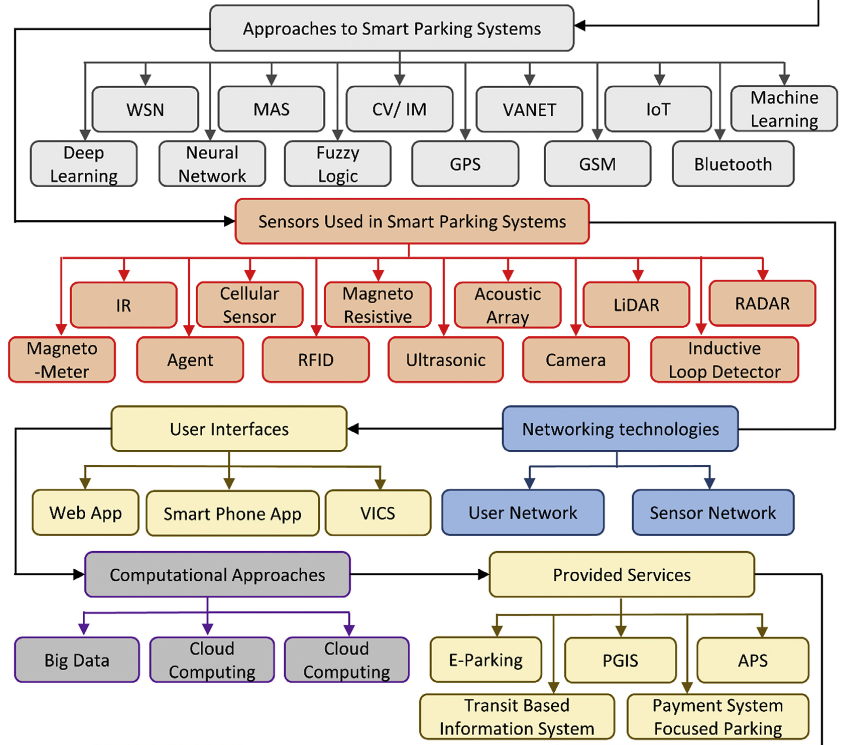
\includegraphics[width=0.9\linewidth]{image/SPS} \caption{Smart Parking (Fahim et al., 2021, p.2)}\label{fig:unnamed-chunk-35}
\end{figure}

Levin et al.~(2020) conclude in their paper on parking infrastructure design for repositioning fully automated vehicles that empty AV repositioning trips (due to lower prices in more distant parking spaces) contribute to network congestion. They have developed a traffic assignment model with endogenous parking choice (where fuel consumption depends on traffic congestion). Since parking choice depends on fuel consumption and parking fees, urban planners can influence reallocation trips by adjusting parking fees. Analysis shows that the genetic algorithm was effective in finding parking options that reduce the impact of empty trips on congestion and reduce the cost of building parking infrastructure in zones with high land values. A similar study by Jiménez et al.~(2022) on perception, positioning and decision-making algorithms for autonomous valet parking using the LiDAR sensor tested in a real parking lot showed promising results with accurate behaviour of the AV. Further studies analyse various autonomous parking systems in different areas (e.g.~urban space, on-street and off-street parking) and with different network positioning. They mostly demonstrate successful technological functionality, while further practicability still needs future testing (Plihal et al., 2022).

Khalid et al.~(2021) summarises the future challenges of SP and AVP as follows:

\begin{itemize}
\tightlist
\item
  Data protection and security

  \begin{itemize}
  \tightlist
  \item
    Secure communication (V2V and V2I)
  \item
    Data protection
  \end{itemize}
\item
  Congestion avoidance

  \begin{itemize}
  \tightlist
  \item
    Routing (the shortest route is not always optimal, as other factors such as price, infrastructure and congestion can also be taken into account depending on the objective)
  \item
    Parking space utilisation (parking space utilisation can be increased but parking will be challenging for normal drivers in car parks for AVs)
  \item
    3D localisation maps (in most car parks the global positioning system (GPS) is not able to locate a free parking space exactly)
  \end{itemize}
\item
  Deployment

  \begin{itemize}
  \tightlist
  \item
    Drop-off and pick-up spot
  \item
    Car park (in remote areas or on the outskirts of the city centre to avoid traffic congestion)
  \end{itemize}
\item
  Scheduling

  \begin{itemize}
  \tightlist
  \item
    Car park scheduling (novel car park scheduling algorithm is needed that takes into account user demand and real-time street information)
  \item
    Vehicle sharing (to further reduce congestion)
  \item
    Charging scheme (efficient charging solutions are required in the planning process to support vehicles, especially in fully automated mode)
  \end{itemize}
\item
  Green parking (improving parking search capacity and reducing journey time can help reduce carbon emissions and pollution)

  \begin{itemize}
  \tightlist
  \item
    Accessibility (reservation, convenient ride, economic/dynamic pricing, hassle-free drop-off and pick-up experience, and green planning and scheduling algorithms)
  \item
    Integrated parking system (degree of integration of various components; built-in GPS, localisation maps of car parks, reservation algorithm, secure payment system and real-time monitoring into the future system)
  \item
    Digitised car parks (With proper management, the number of cars on the road can be reduced and green transport can be realised)
  \end{itemize}
\end{itemize}

\hypertarget{current-state-of-art-in-practice-31}{%
\subsection*{Current state of art in practice}\label{current-state-of-art-in-practice-31}}
\addcontentsline{toc}{subsection}{Current state of art in practice}

The world's first fully automated and driverless car park with SAE Level 4 parking function was officially approved in July 2019 at the Mercedes-Benz Museum in Stuttgart. This project was made possible by \href{https://www.bosch-mobility-solutions.com/en/solutions/parking/automated-valet-parking/}{Bosch} and \href{https://www.daimler.com/innovation/case/autonomous/driverless-parking.html}{Daimler}. The automated drive-up and parking service is accessed via smartphone app and does not require a driver at all. The necessary intelligent parking infrastructure, which supports the mixed traffic of AVP and manually controlled vehicles, comes from Bosch. The technically equipped vehicles come from Mercedes-Benz. Together, the two partners defined the interface between infrastructure and vehicle and adapted the sensor technology and vehicle software accordingly. Due to the sensor technology used in the infrastructure, the necessary equipment of a vehicle is essentially limited to an automatic transmission, ESP, electric parking brake and steering assistance, a start/stop function and the communication unit. The car park system is based on the interaction of intelligent infrastructure and vehicle technology. The necessary car park infrastructure includes the required sensor technology and IT technology to calculate the driving routes and to fulfil all requirements regarding safety. A technical unit that communicates with the vehicle and a cloud connection for interaction with the backend are also required (Robert Bosch GmbH, 2021a). Garages with AVP could have 20\% more capacity, as no space needs to be left for the occupants to exit (Ehrenfeuchter, 2020; Robert Bosch GmbH, 2021a).

Further, AVP garages are planned at Stuttgart Airport and in Detroit (Robert Bosch GmbH, 2021b). Tests have already been carried out in Detroit with Ford Escape test cars (Of-Allinger, 2020). In contrast to earlier test projects, Bosch no longer uses expensive and prominent lidar sensors in the multi-storey car park at Stuttgart Airport, but low-cost cameras. Around 180 of them were mounted on the ceiling. They determine the position of the vehicle ten times per second. A server determines the data and the driving command for the car is calculated and transmitted to the car via Wifi. Thanks to a specially speckled coating, the system also detects possible objects on the floor. If a luggage trolley is in the way, the technology reports the incident and informs an employee. Additionally, in July 2021, Hong Kong revealed its first automated robotic parking system in which robots park vehicles on pallets that then transport the car to a vacant parking space (N. N., 2021).

The Mercedes S-Class is the first series-produced vehicle in the world with AVP technology on board. No additional sensors are required compared to the existing standard technology, but only a special module is necessary to communicate with the car park computer. Potential buyers will be able to order the comfort function in future via the special equipment ``Intelligent Park Pilot''. According to the manufacturer, the costs for this function are in the low four-digit range.

How quickly the technology will spread and how well it will be accepted remains to be seen. However, the advantages are that the sensor technology is not required to be in the car, but rather in the parking garage. This makes it easier for other car manufacturers to use the technology. Bosch is already in intensive talks with other companies. Since the camera infrastructure can simply be installed in a multi-storey car park, the technology will also be usable for older buildings. Modular retrofitting, i.e.~floor by floor, is also possible (Ehrenfeuchter, 2020).

\hypertarget{relevant-initiatives-in-austria-31}{%
\subsection*{Relevant initiatives in Austria}\label{relevant-initiatives-in-austria-31}}
\addcontentsline{toc}{subsection}{Relevant initiatives in Austria}

\begin{itemize}
\tightlist
\item
  \href{https://cms.law/en/int/expert-guides/cms-expert-guide-to-autonomous-vehicles-avs/austria}{Austrian jurisdiction in terms of AV parking}
\end{itemize}

\hypertarget{impacts-with-respect-to-sustainable-development-goals-sdgs-31}{%
\subsection*{Impacts with respect to Sustainable Development Goals (SDGs)}\label{impacts-with-respect-to-sustainable-development-goals-sdgs-31}}
\addcontentsline{toc}{subsection}{Impacts with respect to Sustainable Development Goals (SDGs)}

\begin{longtable}[]{@{}
  >{\centering\arraybackslash}p{(\columnwidth - 8\tabcolsep) * \real{0.2029}}
  >{\centering\arraybackslash}p{(\columnwidth - 8\tabcolsep) * \real{0.1884}}
  >{\centering\arraybackslash}p{(\columnwidth - 8\tabcolsep) * \real{0.2029}}
  >{\centering\arraybackslash}p{(\columnwidth - 8\tabcolsep) * \real{0.2029}}
  >{\centering\arraybackslash}p{(\columnwidth - 8\tabcolsep) * \real{0.2029}}@{}}
\toprule()
\begin{minipage}[b]{\linewidth}\centering
Impact level
\end{minipage} & \begin{minipage}[b]{\linewidth}\centering
Indicator
\end{minipage} & \begin{minipage}[b]{\linewidth}\centering
Impact direction
\end{minipage} & \begin{minipage}[b]{\linewidth}\centering
Goal description and number
\end{minipage} & \begin{minipage}[b]{\linewidth}\centering
Source
\end{minipage} \\
\midrule()
\endhead
Individual & Increased comfort and time saving & \textbf{+} & Health and wellbeing (\emph{3}) & Robert Bosch GmbH (2021b) \\
Systemic & Unpredictable effects on pollution and traffic congestion & \textbf{\textasciitilde{}} & Environmental sustainability (\emph{7,12-13,15}) & Akhavan-Rezai et al., 2018; Khalid et al., 2019 \\
Systemic & Increased collaborations between technology companies and car manufacturers & \textbf{+} & Partnership \& collaborations (\emph{17}) & Ehrenfeuchter, 2020; Of-Allinger, 2020; Robert Bosch GmbH, 2021b \\
\bottomrule()
\end{longtable}

\hypertarget{technology-and-societal-readiness-level-31}{%
\subsection*{Technology and societal readiness level}\label{technology-and-societal-readiness-level-31}}
\addcontentsline{toc}{subsection}{Technology and societal readiness level}

\begin{longtable}[]{@{}cc@{}}
\toprule()
TRL & SRL \\
\midrule()
\endhead
6-8 & 5-7 \\
\bottomrule()
\end{longtable}

\hypertarget{open-questions-29}{%
\subsection*{Open questions}\label{open-questions-29}}
\addcontentsline{toc}{subsection}{Open questions}

\begin{enumerate}
\def\labelenumi{\arabic{enumi}.}
\tightlist
\item
  How well will the technology be adopted?
\item
  How well will the mix work with AVs and manually driven cars in parking infrastructure?
\item
  How error-prone will such parking systems be?
\end{enumerate}

\hypertarget{further-links-27}{%
\subsection*{Further links}\label{further-links-27}}
\addcontentsline{toc}{subsection}{Further links}

\begin{itemize}
\tightlist
\item
  \href{https://www.bosch.com/stories/autonomous-parking-in-parking-garages/}{Bosch}
\item
  \href{https://www.daimler.com/innovation/case/autonomous/driverless-parking.html}{Daimler}
\end{itemize}

\hypertarget{references-31}{%
\subsection*{References}\label{references-31}}
\addcontentsline{toc}{subsection}{References}

\begin{itemize}
\tightlist
\item
  Akhavan-Rezai, E., Shaaban, M. F., El-Saadany, E. F., \& Karray, F. (2018). New EMS to incorporate smart parking lots into demand response. IEEE Transactions on Smart Grid, 9(2), 1376--1386. \url{https://doi.org/10.1109/TSG.2016.2587901}
\item
  Alessandrini, A., Campagna, A., Site, P. D., Filippi, F., \& Persia, L. (2015). Automated vehicles and the rethinking of mobility and cities. Transportation Research Procedia, 5, 145--160. \url{https://doi.org/10.1016/j.trpro.2015.01.002}
\item
  Chirca, M., Chapuis, R., \& Lenain, R. (2015). Autonomous Valet Parking System Architecture. IEEE Conference on Intelligent Transportation Systems, Proceedings, ITSC, 2015-Octob, 2619--2624. \url{https://doi.org/10.1109/ITSC.2015.421}
\item
  Cogill, R., Gallay, O., Griggs, W., Lee, C., Nabi, Z., Ordonez, R., Rufli, M., Shorten, R., Tchrakian, T., Verago, R., Wirth, F., \& Zhuk, S. (2014). Parked cars as a service delivery platform. 2014 International Conference on Connected Vehicles and Expo, ICCVE 2014 - Proceedings, 138--143. \url{https://doi.org/10.1109/ICCVE.2014.7297530}
\item
  Cohen, T., \& Cavoli, C. (2019). Automated vehicles: exploring possible consequences of government (non)intervention for congestion and accessibility. Transport Reviews, 39(1), 129--151. \url{https://doi.org/10.1080/01441647.2018.1524401}
\item
  Cohen, T., Jones, P., \& Cavoli, C. (2017). Social and behavioural questions associated with autonomous vehicles. January, 1--124.
\item
  Ehrenfeuchter, M. (2020, October 14). Automated Valet Parking (AVP): Test am Flughafen Stuttgart \textbar{} AUTO MOTOR UND SPORT. \url{https://www.auto-motor-und-sport.de/tech-zukunft/mobilitaetsservices/automated-valet-parking-flughafen-stuttgart-s-klasse/}
\item
  Fagnant, D. J., \& Kockelman, K. M. (2015). Dynamic ride-sharing and optimal fleet sizing for a system of shared autonomous vehicles. Transportation, 1, 1--16.
\item
  Fahim, A., Hasan, M., Chowdhury, M. A. (2021). Smart parking systems: comprehensive review basen on various aspects. Heliyon. 7(5), e07050, 1-21. \url{https://doi.org/10.1016/j.heliyon.2021.e07050}
\item
  González-González, E., Nogués, S., \& Stead, D. (2020). Parking futures: Preparing European cities for the advent of automated vehicles. Land Use Policy, 91, 104010. \url{https://doi.org/10.1016/j.landusepol.2019.05.029}
\item
  Guerra, E. (2016). Planning for Cars That Drive Themselves: Metropolitan Planning Organizations, Regional Transportation Plans, and Autonomous Vehicles. Journal of Planning Education and Research, 36(2), 210--224. \url{https://doi.org/10.1177/0739456X15613591}
\item
  Heinrichs, D. (2016). Autonomous Driving and Urban Land Use BT - Autonomous Driving: Technical, Legal and Social Aspects (M. Maurer, J. C. Gerdes, B. Lenz, \& H. Winner, Eds.; pp.~213--231). Springer Berlin Heidelberg. \url{https://doi.org/10.1007/978-3-662-48847-8_11}
\item
  Huang, C., Lu, R., Lin, X., \& Shen, X. (2018). Secure automated valet parking: A privacy-preserving reservation scheme for autonomous vehicles. IEEE Transactions on Vehicular Technology, 67(11), 11169--11180. \url{https://doi.org/10.1109/TVT.2018.2870167}
\item
  Jiménez, F., Calvijo, M., Cerrato, A. (2022). Perception, Positioning and Decision-Making Algorithms Adaptation for an Autonomous Valet Parking System Based on Infrastructure Reverence Points Using One Single LiDAR. Sensors. 22(3), 979. \url{https://doi.org/10.3390/s22030979}
\item
  Khalid, M., Cao, Y., Aslam, N., Raza, M., Moon, A., \& Zhou, H. (2019). AVPark: Reservation and cost optimization-based cyber-physical system for long-range autonomous valet parking (L-AVP). IEEE Access, 7, 114141--114153. \url{https://doi.org/10.1109/ACCESS.2019.2930564}
\item
  Khalid, M., Cao, Y., Aslam, N., Suthaputchakun, C., Arshad, M., \& Khalid, W. (2018). Optimized Pricing Scheduling Model for Long Range Autonomous Valet Parking. 2018 International Conference on Frontiers of Information Technology (FIT), 65--70. \url{https://doi.org/10.1109/FIT.2018.00019}
\item
  Khalid, M., Wang, K., Aslam, N., Cao, Y., Ahmad, N., \& Khan, M. K. (2021). From smart parking towards autonomous valet parking: A survey, challenges and future Works. In Journal of Network and Computer Applications (Vol. 175, p.~102935). Academic Press. \url{https://doi.org/10.1016/j.jnca.2020.102935}
\item
  Kuran, M. S., Carneiro Viana, A., Iannone, L., Kofman, D., Mermoud, G., \& Vasseur, J. P. (2015). A smart parking lot management system for scheduling the recharging of electric vehicles. IEEE Transactions on Smart Grid, 6(6), 2942--2953. \url{https://doi.org/10.1109/TSG.2015.2403287}
\item
  Legacy, C., Ashmore, D., Scheurer, J., Stone, J., \& Curtis, C. (2019). Planning the driverless city. Transport Reviews, 39(1), 84--102. \url{https://doi.org/10.1080/01441647.2018.1466835}
\item
  Levin, M. W., Wong, E., Nault-Maurer, B., \& Khani, A. (2020). Parking infrastructure design for repositioning autonomous vehicles. Transportation Research Part C: Emerging Technologies, 120, 102838. \url{https://doi.org/10.1016/j.trc.2020.102838}
\item
  Liu, Z., Xie, Y., Chan, K. Y., Ma, K., \& Guan, X. (2019). Chance-Constrained Optimization in D2D-Based Vehicular Communication Network. IEEE Transactions on Vehicular Technology, 68(5), 5045--5058. \url{https://doi.org/10.1109/TVT.2019.2904291}
\item
  Lou, L., Zhang, J., Xiong, Y., \& Jin, Y. (2019). An improved roadside parking space occupancy detection method based on magnetic sensors and wireless signal strength. Sensors (Switzerland), 19(10). \url{https://doi.org/10.3390/s19102348}
\item
  Manville, M., \& Shoup, D. (2005). Parking, people, and cities. Journal of Urban Planning and Development, 131(4), 233--245. \url{https://doi.org/10.1061/(ASCE)0733-9488(2005)131:4(233)}
\item
  Milakis, D., Snelder, M., Van Arem, B., Van Wee, B., \& De Almeida Correia, G. H. (2017). Development and transport implications of automated vehicles in the Netherlands: Scenarios for 2030 and 2050. European Journal of Transport and Infrastructure Research, 17(1), 63--85. \url{https://doi.org/10.18757/ejtir.2017.17.1.3180}
\item
  Milakis, D., Van Arem, B., \& Van Wee, B. (2017). Policy and society related implications of automated driving: A review of literature and directions for future research. Journal of Intelligent Transportation Systems: Technology, Planning, and Operations, 21(4), 324--348. \url{https://doi.org/10.1080/15472450.2017.1291351}
\item
  N. N. (2021). HKSTP reveals Hong Kong's first automated robotic parking system at science park to advance smart city vision. HKSTP. Available at: \url{https://www.hkstp.org/press-room/hkstp-reveals-hong-kong-s-first-automated-robotic-parking-system-at-science-park-to-advance-smart-city-vision/} {[}Accessed: 24 August 2022{]}
\item
  Ni, J., Lin, X., \& Shen, X. (2019). Toward Privacy-Preserving Valet Parking in Autonomous Driving Era. IEEE Transactions on Vehicular Technology, 68(3), 2893--2905. \url{https://doi.org/10.1109/TVT.2019.2894720}
\item
  Of-Allinger, A. (2020, August 26). Automated Valet Parking von Ford, Bosch und Bedrock \textbar{} AUTO MOTOR UND SPORT. \url{https://www.auto-motor-und-sport.de/tech-zukunft/automated-valet-parking-bosch-ford-bedrock/}
\item
  Pierce, G., \& Shoup, D. (2013). Getting the prices right. Journal of the American Planning Association, 79(1), 67--81. \url{https://doi.org/10.1080/01944363.2013.787307}
\item
  Plihal, J., Nedoma, P., Sestak, V., Herda, Z., Aksjonov, A. (2022). Transport Automation in Urban Mobility: A Case Study of an Autonomous Parking System. Vehicles. 4(2), 326-343. \url{https://doi.org/10.3390/vehicles4020020}
\item
  Porter, L. (2018). The autonomous vehicle revolution: Implications for planning. Planning Theory and Practice, 19(5), 753--778. \url{https://doi.org/10.1080/14649357.2018.1537599}
\item
  Rajabioun, T., \& Ioannou, P. (2015). On-Street and off-street parking availability prediction using multivariate spatiotemporal models. IEEE Transactions on Intelligent Transportation Systems, 16(5), 2913--2924. \url{https://doi.org/10.1109/TITS.2015.2428705}
\item
  Robert Bosch GmbH. (2021a). Automated Valet Parking -- schnell, sicher, fahrerlos \textbar{} Bosch Global. \url{https://www.bosch.com/de/stories/automated-valet-parking/}
\item
  Robert Bosch GmbH. (2021b). Bosch Automated Valet Parking. \url{https://www.bosch-mobility-solutions.com/de/loesungen/parken/automated-valet-parking/}
\item
  Soteropoulos, A., Berger, M., \& Ciari, F. (2019). Impacts of automated vehicles on travel behaviour and land use: an international review of modelling studies. Transport Reviews, 39(1), 29--49. \url{https://doi.org/10.1080/01441647.2018.1523253}
\item
  Wang, D. Z., Posner, I., \& Newman, P. (2015). Model-free detection and tracking of dynamic objects with 2D lidar. International Journal of Robotics Research, 34(7), 1039--1063. \url{https://doi.org/10.1177/0278364914562237}
\item
  Williams, L. (2019). The whole story of parking: The world of parking is no longer stationary. Eng. Technol., 14(2), 56--61.
\item
  Winter, S., Salil, G. (2021). Smart Parking in Fast-Growing Cities. Challenges and Solutions. TU Wien Academic Press. ISBN: 978-3-85448-045-7. DOI: 10.34727/2021/isbn.978-3-85448-045-7. Available at: \url{https://repositum.tuwien.at/bitstream/20.500.12708/18055/1/Winter-2021-SMART\%20PARKING\%20IN\%20FAST-GROWING\%20CITIES-vor.pdf} {[}Accessed: 22 August 2022{]}
\item
  Zakharenko, R. (2016). Self-driving cars will change cities. Regional Science and Urban Economics, 61, 26--37. \url{https://doi.org/10.1016/j.regsciurbeco.2016.09.003}
\item
  Zhang, W. (2017). the Interaction Between Land Use and Transportation in the Era of Shared Autonomous Vehicles: a Simulation Model. August, 147.
\item
  Zhang, W., Guhathakurta, S., Fang, J., \& Zhang, G. (2015). Exploring the impact of shared autonomous vehicles on urban parking demand: An agent-based simulation approach. Sustainable Cities and Society, 19, 34--45. \url{https://doi.org/10.1016/j.scs.2015.07.006}
\item
  Zhou, D., Yan, Z., Fu, Y., \& Yao, Z. (2018). A survey on network data collection. Journal of Network and Computer Applications, 116, 9--23. \url{https://doi.org/10.1016/j.jnca.2018.05.004}
\end{itemize}

\hypertarget{automated_road_freight}{%
\section{Automated road freight}\label{automated_road_freight}}

\textbf{Updated: 26th August 2022}

\hypertarget{synonyms-28}{%
\subsection*{Synonyms}\label{synonyms-28}}
\addcontentsline{toc}{subsection}{Synonyms}

\emph{automated driving systems (ADS), combustion-powered heavy vehicles (CHV), battery electric heavy vehicles (BEHVs), cooperative and automated vehicles (CAVs)}

\hypertarget{definition-32}{%
\subsection*{Definition}\label{definition-32}}
\addcontentsline{toc}{subsection}{Definition}

The transport sector will soon experience a revolution in automated driving systems (ADS), as reported by Wadud et al.~(2016) and Flämig (2016). Some benefits in terms of user experience, efficiency, safety, mobility, productivity, energy, environment and economy have been reported with ADS by many studies (Alessandrini et al., 2015; Anderson et al., 2016; Brown et al., 2014; Chan, 2017; Harper et al., 2016; Wadud, 2017; Kopelias et al., 2020 and Khan et al., 2019), although significant increases in road safety from highly or fully automated vehicles are not certain, as shown by Kalra \& Paddock (2016).

The goals and motivations of automated driving for passenger cars and freight transport differ greatly (Wadud, 2017; Nowakowski et al., 2015). For passenger cars, the main motivations are user experience and the environment, while for freight, the main drivers are productivity and profitability. For example, the increase in the cost of a vehicle related to automation hardware is less important in freight transport due to the lower share of automation hardware costs in the total acquisition costs compared to those of passenger cars. In addition, ADS enable higher profitability in freight transport, mainly due to a reduction in labour costs as well as facilitated logistics and increased utilisation and efficiency (Wadud et al., 2016). In addition, driver costs decrease significantly with high or full automation of driving, leading to early adoption of ADS in the freight sector (Ghandriz et al., 2020a).

The levels of automation are currently divided into 5 levels (Paulsen, 2018):

\textbf{First level: assisted driving}

Individual assistance systems provide support for specific driving tasks. Assisted driving is already a reality in many cars today. (see automatic adaptive cruise control and automatic lane departure warning).

\textbf{Second level: partially automated driving}

With semi-automated driving, the car/truck can temporarily perform some tasks itself, without any human intervention. For this purpose, various individual systems are combined with each other, in this case, the automatic adaptive cruise control with the emergency braking and lane departure warning systems. Further level 2 functions include overtaking assistant, automatic parking.

\textbf{Third level: highly automated driving}

Highly automated cars/trucks (Level 3) can perform certain driving tasks autonomously and without human intervention, but only for a limited period of time and under suitable conditions specified by the manufacturer. Level 3 cars will probably be on the road on motorways first: There is no oncoming traffic there, the lane markings are usually in order, and the roads are continuously recorded as digital maps. Since 2017, there has also been a legal framework for Level 3 cars in Germany: as soon as the driver puts his car into highly automated mode, he is allowed to turn his attention away from the road traffic. This means that the driver is allowed to read the newspaper.
However, if the system detects a problem and sends a signal, the driver must take over the wheel immediately.

\textbf{Level four: fully automated driving}

In the development departments of the large car companies, but also at Apple, Google or Uber, engineers and computer scientists are working flat out on the full automation of the car, i.e.~level 4 on the way to autonomous driving. In this level, the technical systems carry out all driving tasks automatically, and the car can also cover longer distances without intervention.
So far, however, there is no legal framework for fully automated vehicles.

\textbf{Fifth level: autonomous driving}

The fifth is the final level of autonomous driving. The car is now completely guided by the system and performs all the necessary tasks automatically. Even complex situations - such as crossing an intersection, driving through a roundabout or the correct behaviour at a zebra crossing - can be handled by the autonomous car.

For a regulatory framework, seamless and harmonised cross-border EU and national regulation of automated road transport is seen by the European Commission, 2019 as a key factor for market introduction. Common procedures for testing, validation and certification enable the standardisation of solutions. Standards should also apply to data exchange and communication solutions. Ethical, legal, environmental and safety aspects should be regulated. The liability and responsibility of each actor in the road system must be defined before the introduction of automated driving.

\hypertarget{key-stakeholders-32}{%
\subsection*{Key stakeholders}\label{key-stakeholders-32}}
\addcontentsline{toc}{subsection}{Key stakeholders}

\begin{itemize}
\tightlist
\item
  \textbf{Affected}: Truck drivers, Freight forwarders, Delivery companies
\item
  \textbf{Responsible}: National Governments, City government, Freight forwarders, Delivery companies
\end{itemize}

\hypertarget{current-state-of-art-in-research-32}{%
\subsection*{Current state of art in research}\label{current-state-of-art-in-research-32}}
\addcontentsline{toc}{subsection}{Current state of art in research}

The reduction in fuel consumption achieved with ADS due to improved vehicle use and controlled energy management is only up to 10\% for passenger cars compared to when a human driver is involved, depending on the traffic scenario (Mersky \& Samaras, 2016). The reduction in fuel consumption achieved with ADS is likely to be higher in freight transport, considering that heavy vehicles can form platoons, which theoretically reduce the energy intensity of the following vehicle by up to 25\% when the distance between vehicles reaches zero, according to (Wadud et al., 2016); while measurements showed average fuel savings of 8\% and 15\% for 10 m and 4 m distance of the trucks in the platoon, respectively, according to (Tsugawa et al., 2016). However, as the European Commission (2016) points out, heavy-duty vehicles contribute to about 25 \% of CO2 emissions from road transport in Europe, which are rising due to increasing road freight transport despite improved fuel efficiency. These figures suggest that the efficiency improvements offered by ADS, although a profitable business, cannot lead to a reduction in CO2 emissions in the long term; therefore, a further reduction of emissions in the transport sector is needed, motivating the development of greener solutions (Ghandriz et al., 2020a).

In a slightly simplified study of ADS in heavy vehicles, a reduction in the total cost of ownership (TCO) of trucks of between 27\% and 46\% for battery electric heavy vehicles (BEHVs) and between 11\% and 41\% for combustion-powered heavy vehicles (CHVs) makes BEHVs more profitable than BEHVs with human drivers by a factor of four over longer distances. It was observed that Level 4-5 automated BEHVs tend to have lower optimal speeds than vehicles with human drivers. Furthermore, it was shown that reducing speed for safety reasons is less costly to implement for Level 4-5 automated BEHVs than for Level 4-5 automated CHVs; in many scenarios, low speeds up to 60 km/h even reduced the TCO. The reduction in TCO in Level 4-5 automated trucks was mainly achieved by eliminating driver pay (35\%-55\%), the increase of the operating time on the road and thus the reduction of the downtimes (0\%-15\%), increasing payload by eliminating the cab (1.2\%-5\%), and optimising the drive system (0\%-20\%) (Ghandriz et al., 2020a). All the data and figures obtained were made available in (Ghandriz et al., 2020b) and provide valuable information on the feasibility and profitability of a planned freight transport operation with automation and electrification for a specific use case.

Pribyl et al., (2020) are investigating the effects of lower CAV penetrations. According to this, even with a low number of CAVs on the roads, the impact on transport and environmental performance indicators will be significant. However, this integration needs to be combined with other measures and policies such as the promotion of alternative powertrains if EU emission targets are to be met. However, results have also shown that CAVs can negatively affect other traffic parameters and lead, for example, to delays and other traffic flow phenomena.

Shin et al., (2018) analyse some of the technical trends related to intermodal automated freight transport systems (ATFS) that aim to reduce greenhouse gases and particulate matter, minimise infrastructure costs and logistics costs, and alleviate traffic congestion. Countries such as the US, Germany, the Netherlands and Japan have been actively developing technologies for ATFS.
Gan et al., 2021 capture the characteristics of the swarm intelligence of truck drivers as a solid basis for the design, control and management of the future driverless truck swarm robotics system. The detection of the short-term location of truck drivers in advance, especially for areas with high freight demand, and thus the optimal use of freight capacity on the motorway, is the key component of freight matching. For city-level forecasting, it can help to determine the city points that truckers will be driving to, making it easier to plan an optimal route for them from the city's perspective. It can also predict the internal transport capacity of the city, predict the bottleneck caused by the truck and provide decisions for inner-city traffic management.

Mulholland et al., (2018) define a global assessment of the decarbonisation of road freight transport by 2050. Overall, global road freight transport in tonnes-kilometer (tkm) is projected to grow 2.4-fold over the period 2015-2050 in their Reference Technology Scenario (RTS), with developing countries accounting for most of the growth, in line with economic growth. Developing countries are projected to account for 75\% of road freight transport in 2050. In order to reduce dependence on fossil fuels, three key requirements are proposed:

\begin{itemize}
\tightlist
\item
  Fuel economy standards (minimum efficiency)
\item
  Support for comprehensive data collection and information exchange
\item
  Promoting the use of alternative fuels and the vehicles that use them
\end{itemize}

Recent research developed models to optimise the routing of freight (Sharma et al., 2022) as well as combining various modes of transport (Dekhtyaruk et al., 2021), simulations of mixed traffic (Chaudhry, 2022) and driver behaviour and experiences around automated freight vehicle platoons (Yang et al., 2022; Paddeu and Denby, 2022). Nonetheless, there is still uncertainty expected with most of the research, depending on the used model, area and implementation characteristics. Increasing research however, points towards awareness to use automation for freight to increase safety and decrease carbon use, while further optimising routes, platooning and mixed traffic solutions.

\hypertarget{current-state-of-art-in-practice-32}{%
\subsection*{Current state of art in practice}\label{current-state-of-art-in-practice-32}}
\addcontentsline{toc}{subsection}{Current state of art in practice}

The initial introduction of fully automated driving in closed traffic systems (e.g.~traffic in a system network) and manageable scenarios (e.g.~motorway, airport grounds, ports) helps to overcome the reluctance towards the technologies as well as the lack of standardisation. The gradual introduction of platooning, starting with manned lead and follow vehicles, could build up the necessary acceptance among the population. It should be examined whether the simultaneous introduction of overhead electric trucks and thus the creation of a dedicated lane would make sense in terms of capacity and safety requirements (Flämig, 2016).

A European Commission, 2019 report contained many automated road projects, but only one deals specifically with freight transport:

\begin{itemize}
\tightlist
\item
  Ensemble (01/06/2018- 31/05/2021)
\end{itemize}

The project aims to support the implementation of multi-brand truck platooning on European roads, so that a single truck can form a platoon with any other truck.

Other projects may have approached the issue in a different way, but the focus was on all vehicles. For example:

\begin{itemize}
\tightlist
\item
  Headstart (01/01/2019- 31/12/2021)
\end{itemize}

The project aims to define test and validation procedures for specific functionalities of Connected and Automated Driving (CAD), including key technologies such as communication, cyber security and positioning. The tests will take place both in simulation and in the real world to validate safety and security performance.

\begin{itemize}
\tightlist
\item
  Levitate (01/12/2018- 30/11/2021)
\end{itemize}

The project will develop a wide-ranging assessment framework to evaluate the impact of connected and automated transport (CAT) on all aspects of transport and individual mobility, as well as at a societal level. The project addresses the needs of local authorities, regional authorities and national governments to prepare for the increasing use of connected and automated systems, to understand the implications for mobility policy and to take the most effective measures to achieve broader societal goals.

Furthermore, the European Commission (2022) presents many automated road projects as well as urban freight transport policies and research funding within the Horizon 2020 (H2020) research program (Lozzi et al., 2018). Research and projects specifically addressing automated freight transport includes only a handful, mainly dealing with logistics planning and scheduling as well as \href{https://www.euspa.europa.eu/system/files/reports/galileoforautonomousdriving2017a.pdf}{Galileo-based} solutions while main research and projects deal with rail automation and automation in road transport in general (European Commission, 2022).

In the US four manufacturers that dominate the US long-haul truck market have all begun to look at a driverless future. In 2019-2021, each of them has signed contracts with one of the three leading developers of self-driving vehicles (Alphabet's Waymo, TuSimple Holdings and Aurora Innovation). Aurora plans to sell its driverless technology as a service, similar to the way jet engine makers charge airlines for hours spent on the throttle. TuSimple and Waymo Via have similar plans and are also operating cargo services while they test their technology. None of the partnerships with manufacturers are exclusive. The flurry of activity around trucking reflects a growing consensus that self-driving cars are still a long way from reaching most roads, and that 18-wheel trucks might be a better application area to establish the technology. Long-haul trucks drive straight most of the time on highways without traffic lights, cyclists or pedestrians crossing the road (Boudway, 2021).

Self-driving vehicles could have an immense impact on logistics and supply chain management. This is because fully automated trucks, last-mile delivery robots and other AVs fit into an increasingly automated distribution process. The automation of high-volume freight routes has the potential to deliver huge efficiency gains in terms of improved safety, increased capacity, lower operating costs and reduced environmental impact. An analyst at Gartner predicts that while self-driving trucks won't be commercially available until 2024 at the earliest, supply chain executives responsible for transportation should start preparing for a fully automated future now. After all, fully automated trucks are just one part to fully automating the entire supply chain, from fully automated inventory planning to fully automated shipping to fully automated distribution. In a report (March 2021), a market research firm predicted that fully automated trucks will be more widely deployed by 2030, accounting for more than 10\% of new heavy-duty truck sales on the road. By 2028, one-fifth of the world's countries will have active regulations allowing the legal operation of production-ready fully automated vehicles, up from zero in 2019 (Eddy, 2021).

\textbf{Societal aspect}

Despite the imminent technical possibility of implementation, society may not be quite ready for it and political opposition because of the potential for large-scale unemployment among commercial drivers is expected (Wadud, 2017). Whereas, according to the IRU (International Road Transport Union), the European road transport sector is facing the biggest shortage of professional drivers in decades in 2019. According to a survey, the reasons are: the lack of attracting women to work in transport (female drivers make up only 2 per cent of employees in the European transport sector), attracting young people to work in the industry, the poor image of the profession, poor working conditions and being away from home and family for too long. In addition, there is the demographic ageing of the workforce. The average age of a truck driver in Europe is 44 (Kulikowska-Wielgus, 2019).

In the US, federal agencies have filed plans with the Office of Management and Budget (OMB) for a survey study to assess public appetite for automated driving systems (ADS) in the trucking sector. However, the project, Trucking Fleet Concept of Operations (CONOPS) for Managing Mixed Fleets, has already received public pressure. While the Federal Motor Carrier Safety Administration (FMCSA) received only eight comments on the proposal when it was first requested in November, all opposed it. They cited the ``potential loss of jobs for truck drivers and safety concerns arising from ADS testing in the real world'' before enough simulator testing has been done. ``People who rely on truck driving jobs will become unemployed and will no longer have a way to earn a living and provide for themselves and their families,'' one comment stated. If OMB approves the survey, a questionnaire will be completed before and after participants have the opportunity to have hands-on experience with ADS truck technology to assess a change in sentiment. The plan is to share these experiences at four ``road shows'' at existing trucking conferences around the country (Gallagher, 2021). Recently, \href{https://www.tusimple.com/}{TuSimple}, a start-up building technology specifically designed for autonomous trucks signed their first contract with Union Pacific, to coordinate their freight shipments in Arizona, while they continue their test operations in Arizona and Texas, being ahead of most companies in this sector (Doll, 2022; Fisher, 2022).

Since 2019, a fully electric fully automated truck ``T-Pod'' from Einride has been driving on a public road in Sweden on behalf of logistics service provider DB Schenker. However, the approval, which was valid until the end of 2020, stipulated that the T-Pod, which weighs up to 26 tonnes, may only travel at 5 km/h, that the approval was only valid for a specific public road in an industrial area and that one employee was assigned to each vehicle as a supervisor who can intervene from a distance via joystick in the event of problems. The truck was highly technical did not have a driver's cab. According to Einride, the e-truck offers space for 15 Euro pallets instead. Its regular maximum speed is capped at 85 km/h. A 280 kWh battery on board is supposed to guarantee a range of 200 km (Of-Allinger et al., 2020; Werwitzke, 2019).

In manageable, closed areas such as quarries or mines driverless vehicles are already being tested in practice. Volvo Trucks, for example, has six self-driving trucks in operation at a Norwegian limestone plant (Böhm, 2019).

\hypertarget{relevant-initiatives-in-austria-32}{%
\subsection*{Relevant initiatives in Austria}\label{relevant-initiatives-in-austria-32}}
\addcontentsline{toc}{subsection}{Relevant initiatives in Austria}

In Upper Austria (Gunskirchen), a driverless truck will soon also be on the road in public areas. Over the next three years, it will regularly cover the approximately 600-metre route between the logistics centre of DB Schenker Austria and the engine manufacturer BRP-Rotax. The route runs partly on factory premises and partly in public areas and is to be completed in all weathers. After completion of the test phase, the driverless electric transporter will then cover the route between DB Schenker's logistics centre and the BRP-Rotax company, which is mainly on the public road, completely autonomously from 2023. The electric vehicle is to complete the route in all weathers, whether wind, rain or snow. For freight transport, a classic diesel truck currently travels the same route several times a day (APA, 2021; DB, 2021).

\begin{itemize}
\tightlist
\item
  \href{https://www.land-oberoesterreich.gv.at/248885.htm}{Land-oberoesterreich.gv.at}
\end{itemize}

\hypertarget{impacts-with-respect-to-sustainable-development-goals-sdgs-32}{%
\subsection*{Impacts with respect to Sustainable Development Goals (SDGs)}\label{impacts-with-respect-to-sustainable-development-goals-sdgs-32}}
\addcontentsline{toc}{subsection}{Impacts with respect to Sustainable Development Goals (SDGs)}

\begin{longtable}[]{@{}
  >{\centering\arraybackslash}p{(\columnwidth - 8\tabcolsep) * \real{0.2029}}
  >{\centering\arraybackslash}p{(\columnwidth - 8\tabcolsep) * \real{0.1884}}
  >{\centering\arraybackslash}p{(\columnwidth - 8\tabcolsep) * \real{0.2029}}
  >{\centering\arraybackslash}p{(\columnwidth - 8\tabcolsep) * \real{0.2029}}
  >{\centering\arraybackslash}p{(\columnwidth - 8\tabcolsep) * \real{0.2029}}@{}}
\toprule()
\begin{minipage}[b]{\linewidth}\centering
Impact level
\end{minipage} & \begin{minipage}[b]{\linewidth}\centering
Indicator
\end{minipage} & \begin{minipage}[b]{\linewidth}\centering
Impact direction
\end{minipage} & \begin{minipage}[b]{\linewidth}\centering
Goal description and number
\end{minipage} & \begin{minipage}[b]{\linewidth}\centering
Source
\end{minipage} \\
\midrule()
\endhead
Individual & ADS in heavy vehicles lead to a reduction in the total cost of ownership of trucks of between 11\% and 46\% & \textbf{+} & Sustainable economic development (\emph{8,11}) & Ghandriz et al., 2020a \\
Systemic & Reduction in the environmental impact & \textbf{+} & Environmental sustainability (\emph{7,12-13,15}) & Kopelias et al., 2020 \\
Systemic & ADS enable higher profitability in freight transport & \textbf{+} & Sustainable economic development (\emph{8,11}) & Wadud et al., 2016 \\
Systemic & The C-ROADS platform was established to harmonise the use of C-ITS activities across Europe & \textbf{+} & Partnership \& collaborations (\emph{17}) & European Commission, 2021 \\
\bottomrule()
\end{longtable}

\hypertarget{technology-and-societal-readiness-level-32}{%
\subsection*{Technology and societal readiness level}\label{technology-and-societal-readiness-level-32}}
\addcontentsline{toc}{subsection}{Technology and societal readiness level}

\begin{longtable}[]{@{}cc@{}}
\toprule()
TRL & SRL \\
\midrule()
\endhead
6-8 & 5-7 \\
\bottomrule()
\end{longtable}

\hypertarget{open-questions-30}{%
\subsection*{Open questions}\label{open-questions-30}}
\addcontentsline{toc}{subsection}{Open questions}

\begin{enumerate}
\def\labelenumi{\arabic{enumi}.}
\tightlist
\item
  How significant will the rebound effect be that results from the improvement in freight efficiency? Should other technologies/modes of transport, therefore, be preferred?
\item
  Who is responsible if the technology in semi-automated mode violates a speed limit or other traffic regulations?
\item
  How should commercial CAVs best be integrated with conventional trucks?
\end{enumerate}

\hypertarget{further-links-28}{%
\subsection*{Further links}\label{further-links-28}}
\addcontentsline{toc}{subsection}{Further links}

\begin{itemize}
\tightlist
\item
  \href{https://ec.europa.eu/inea/en/horizon-2020/automated-road-transport}{ec.europa.eu}
\end{itemize}

\hypertarget{references-32}{%
\subsection*{References}\label{references-32}}
\addcontentsline{toc}{subsection}{References}

\begin{itemize}
\tightlist
\item
  Alessandrini, A., Campagna, A., Site, P. D., Filippi, F., \& Persia, L. (2015). Automated vehicles and the rethinking of mobility and cities. Transportation Research Procedia, 5, 145--160. \url{https://doi.org/10.1016/j.trpro.2015.01.002}
\item
  Anderson, J., Kalra, N., Stanley, K., Sorensen, P., Samaras, C., \& Oluwatola, O. (2016). Autonomous Vehicle Technology: A Guide for Policymakers. In Autonomous Vehicle Technology: A Guide for Policymakers. \url{https://doi.org/10.7249/rr443-2}
\item
  APA. (2021). Selbstfahrender Lkw in OÖ unterwegs \textbar{} SN.at. Salzburger Nachrichten. \url{https://www.sn.at/wirtschaft/oesterreich/selbstfahrender-lkw-in-ooe-unterwegs-99060673}
\item
  Böhm, M. (2019, November 5). Selbstfahrende Lkws: Die Autonomen rollen an - Transport \& Logistik - derStandard.at › Wirtschaft. \url{https://www.derstandard.at/story/2000110697906/selbstfahrende-lkws-die-autonomen-rollen-an}
\item
  Boudway, I. (2021, May 5). Supply Chains Latest: Driverless Trucks a Deal Closer to Freeway. - Bloomberg. Bloomberg. \url{https://www.bloomberg.com/news/newsletters/2021-05-05/supply-chains-latest-driverless-trucks-a-deal-closer-to-freeway}
\item
  Brown, A., Gonder, J., \& Repac, B. (2014). An Analysis of Possible Energy Impacts of Automated Vehicles BT - Road Vehicle Automation (G. Meyer \& S. Beiker (eds.); pp.~137--153). Springer International Publishing. \url{https://doi.org/10.1007/978-3-319-05990-7_13}
\item
  Chan, C. Y. (2017). Advancements, prospects, and impacts of automated driving systems. International Journal of Transportation Science and Technology, 6(3), 208--216. \url{https://doi.org/10.1016/j.ijtst.2017.07.008}
\item
  Chaudhry, A., Sha, H., Haouari, R., Quddus, M., Thomas, P., Boghani, H., Weigermars, W., Gebhard, S., Sigh, M. K., Morris, A. (2022). Evaluating the Network-Level Road Safety Impacts of Connected and Automated Vehicles in Mixed Traffic Using Traffic Microsimulation Methods. Transport Research Board. Conference: 101st Annual Meeting. Available at: \url{https://trid.trb.org/view/1909507} {[}Accessed: 24 August 2022{]}
\item
  DB. (2021, March 16). Autonomes Fahren: DB Schenker und BRP-Rotax starten Testbetrieb in Österreich. \url{https://www.dbschenker.com/at-de/ueber-uns/presse/corporate-news/autonomes-fahren--db-schenker-und-brp-rotax-starten-testbetrieb-in-oesterreich-688986}
\item
  Dekhtyaruk, M. T., Shao, M., Yang, S., Kontrobayeva, Z. D., Vashchilina, E. (2021). Automated system of freight traffic optimisation in the interaction of various modes of transport. Periodicals of Engineering and Natural Sciences. 9(3). \url{http://dx.doi.org/10.21533/pen.v9i3.2320}
\item
  Doll, S. (2022). Union Pacific becomes TuSimple's first fully-autonomous truck customer, moving freight between rail and first/last mile without a driver. Electrek. Available at: \url{https://electrek.co/2022/02/02/union-pacific-becomes-tusimples-first-fully-autonomous-trucking-customer-moving-freight-between-rail-and-first-last-mile-without-a-driver/} {[}Accessed: 24 August 2022{]}
\item
  Eddy, N. (2021, May 8). Driverless trucks worth the long-term investment -- Urgent Comms. \url{https://urgentcomm.com/2021/05/10/driverless-trucks-worth-the-long-term-investment/}
\item
  European Commission. (2019). Automated road transport.
\item
  European Commission. (2021, April 30). Connected and automated mobility \textbar{} Shaping Europe's digital future. \url{https://digital-strategy.ec.europa.eu/en/policies/connected-and-automated-mobility}
\item
  European Commission. (2022). European Climate Infrastructure and Environment Executive Agency (CINEA). Projects: Transport and Mobility (Horizon 2020). Available at: \url{https://cinea.ec.europa.eu/our-projects_en} {[}Accessed: 24 August 2022{]}
\item
  Fisher, J. (2022). As excitement of self-driving trucks grows, fleets will soon have products to choose from. FleetOwner: Technology. Available at: \url{https://www.fleetowner.com/technology/article/21213982/as-excitement-of-selfdriving-trucks-grows-fleets-will-soon-have-products-to-choose-from} {[}Accessed 24 August 2022{]}
\item
  Flämig, H. (2016). Autonomous vehicles and autonomous driving in freight transport. In Autonomous Driving: Technical, Legal and Social Aspects (pp.~365--385). Springer Berlin Heidelberg. \url{https://doi.org/10.1007/978-3-662-48847-8_18}
\item
  Gallagher, J. (2021, April 23). FMCSA automated trucks project headed to White House - FreightWaves. Freightwaves. \url{https://www.freightwaves.com/news/fmcsa-automated-trucks-project-headed-to-white-house}
\item
  Gan, M., Qian, Q., Li, D., Ai, Y., \& Liu, X. (2021). Capturing the swarm intelligence in truckers: The foundation analysis for future swarm robotics in road freight. Swarm and Evolutionary Computation, 62, 100845. \url{https://doi.org/10.1016/j.swevo.2021.100845}
\item
  Ghandriz, T., Jacobson, B., Laine, L., \& Hellgren, J. (2020a). Impact of automated driving systems on road freight transport and electrified propulsion of heavy vehicles. Transportation Research Part C: Emerging Technologies, 115, 102610. \url{https://doi.org/10.1016/j.trc.2020.102610}
\item
  Ghandriz, T., Jacobson, B., Laine, L., \& Hellgren, J. (2020b). Optimization data on total cost of ownership for conventional and battery electric heavy vehicles driven by humans and by automated driving systems. Data in Brief, 30. \url{https://doi.org/10.1016/j.dib.2020.105566}
\item
  Harper, C. D., Hendrickson, C. T., \& Samaras, C. (2016). Cost and benefit estimates of partially-automated vehicle collision avoidance technologies. Accident Analysis and Prevention, 95, 104--115. \url{https://doi.org/10.1016/j.aap.2016.06.017}
\item
  Kalra, N., \& Paddock, S. M. (2016). Driving to safety: How many miles of driving would it take to demonstrate autonomous vehicle reliability? Transportation Research Part A: Policy and Practice, 94, 182--193. \url{https://doi.org/10.1016/j.tra.2016.09.010}
\item
  Khan, A., Harper, C. D., Hendrickson, C. T., \& Samaras, C. (2019). Net-societal and net-private benefits of some existing vehicle crash avoidance technologies. Accident Analysis and Prevention, 125, 207--216. \url{https://doi.org/10.1016/j.aap.2019.02.003}
\item
  Kopelias, P., Demiridi, E., Vogiatzis, K., Skabardonis, A., \& Zafiropoulou, V. (2020). Connected \& autonomous vehicles -- Environmental impacts -- A review. Science of the Total Environment, 712, 135237. \url{https://doi.org/10.1016/j.scitotenv.2019.135237}
\item
  Kulikowska-Wielgus, A. (2019, March 28). Every fifth truck driver position in Europe is vacant. Soon, there could be twice as many. - Trans.INFO. Trans.Info. \url{https://trans.info/en/every-fifth-truck-driver-position-in-europe-is-vacant-soon-there-could-be-twice-as-many-131212}
\item
  Lozzi, G., Gatta, V. Marcucci, E. (2018). European urban freight transport policies and funding: Are priorities and Horizon 2020 calls aligned. Region. 5(1), 53-71. DOI: 10.18335/region.v5i1.168
\item
  Mersky, A. C., \& Samaras, C. (2016). Fuel economy testing of autonomous vehicles. Transportation Research Part C: Emerging Technologies, 65, 31--48. \url{https://doi.org/10.1016/j.trc.2016.01.001}
\item
  Mulholland, E., Teter, J., Cazzola, P., McDonald, Z., \& Ó Gallachóir, B. P. (2018). The long haul towards decarbonising road freight -- A global assessment to 2050. Applied Energy, 216, 678--693. \url{https://doi.org/10.1016/j.apenergy.2018.01.058}
\item
  Nowakowski, C., Shladover, S. E., \& Tan, H. S. (2015). Heavy Vehicle Automation: Human Factors Lessons Learned. Procedia Manufacturing, 3, 2945--2952. \url{https://doi.org/10.1016/j.promfg.2015.07.824}
\item
  Of-Allinger, A., Knecht, J., \& Conrad, B. (2020, April 30). Automomer Elektro-Lkw Einride T-Pod: Zulassung in Schweden \textbar{} AUTO MOTOR UND SPORT. Auto Motr Sport. \url{https://www.auto-motor-und-sport.de/elektroauto/automomer-elektro-lkw-einride-t-pod-strassenzulassung/}
\item
  Paddeu, D., Denby, J. (2022). Decarbonising road freight: Is truck automation and platooning an opportunity?. Clean Technologies and Environmental Policy. 24, 2021-1035. \url{https://doi.org/10.1007/s10098-020-02020-9}
\item
  Paulsen, T. (2018, November 7). Autonomes Fahren: 5 Level zum selbstfahrenden Auto \textbar{} ADAC. ADAC. \url{https://www.adac.de/rund-ums-fahrzeug/ausstattung-technik-zubehoer/autonomes-fahren/grundlagen/autonomes-fahren-5-stufen/}
\item
  Pribyl, O., Blokpoel, R., \& Matowicki, M. (2020). Addressing EU climate targets: Reducing CO\textsubscript{2} emissions using cooperative and automated vehicles. Transportation Research Part D: Transport and Environment, 86, 102437. \url{https://doi.org/10.1016/j.trd.2020.102437}
\item
  Sharma, S., van Lint, H., Tavasszy, L., Snelder, M. (2022). Estimating Route Choice Characteristics of Truck Drivers from Sparse Automated Vehicle Identification Data through Data Fusion and Bi-Objective Optimization. Transportation Research Record: Journal of the Transportation Research Board. \url{https://doi.org/10.1177/03611981221095089}
\item
  Shin, S., Roh, H. S., \& Hur, S. H. (2018). Technical Trends Related to Intermodal Automated Freight Transport Systems (AFTS) *. Asian Journal of Shipping and Logistics, 34(2), 161--169. \url{https://doi.org/10.1016/j.ajsl.2018.06.013}
\item
  Tsugawa, S., Jeschke, S., \& Shladovers, S. E. (2016). A review of truck platooning projects for energy savings. IEEE Transactions on Intelligent Vehicles, 1(1), 68--77. \url{https://doi.org/10.1109/TIV.2016.2577499}
\item
  Wadud, Z. (2017). Fully automated vehicles: A cost of ownership analysis to inform early adoption. Transportation Research Part A: Policy and Practice, 101, 163--176. \url{https://doi.org/10.1016/j.tra.2017.05.005}
\item
  Wadud, Z., MacKenzie, D., \& Leiby, P. (2016). Help or hindrance? The travel, energy and carbon impacts of highly automated vehicles. Transportation Research Part A: Policy and Practice, 86, 1--18. \url{https://doi.org/10.1016/j.tra.2015.12.001}
\item
  Werwitzke, C. (2019, May 17). Schweden: T-Pod erhält Zulassung für öffentliche Straße - electrive.net. Electrive.Net. \url{https://www.electrive.net/2019/05/17/schweden-t-pod-erhaelt-zulassung-fuer-oeffentliche-strasse/}
\item
  Yang, S., Park, J., Abdel-Aty, M. (2022). Driver behaviour and experiences around automated freight vehicle platoons. Transport. ICE Publishing. \url{https://doi.org/10.1680/jtran.22.00039}
\end{itemize}

\hypertarget{automatic_train}{%
\section{Automatic train operations}\label{automatic_train}}

\textbf{Updated: 29th August 2022}

\hypertarget{synonyms-29}{%
\subsection*{Synonyms}\label{synonyms-29}}
\addcontentsline{toc}{subsection}{Synonyms}

\emph{high-speed railways (HSR), automatic train control system (ATC), Grade of Automation (GoA), unattended train operation (UTO or GoA4)}

\hypertarget{definition-33}{%
\subsection*{Definition}\label{definition-33}}
\addcontentsline{toc}{subsection}{Definition}

Over the past decades, rail transport systems have undergone significant changes in terms of technology level, overall length, travel speed and service qualities. The management of train operations to achieve safe and efficient operation for a railway system has been a long-term concern. In traditional railway systems, this is usually achieved by \emph{(i)} a timetable and a vehicle plan and \emph{(ii)} real-time train operation by drivers using fixed signalling equipment. However, this partially manual work has many disadvantages for train operation due to increasing traffic demand and limited railway infrastructure. Manual driving is usually based on training and experience, which lacks rigorous calculations and systematic considerations. Therefore, it is difficult to ensure safety, quality of service (e.g.~transport capacity, punctuality, accuracy of stops) and operating costs (e.g.~energy consumption, infrastructure utilisation). This problem is particularly serious in urban rail systems, where passenger demand is extremely high and train departure times are very short (Yin et al., 2017).

In manual operation, drivers must keep track of the forward signals and then give appropriate train control commands. Essentially, the track logic and dispatchers only know which track circuit the train is on and prevent other trains from entering the same track circuit. Furthermore, as this process is not strictly monitored and rigorously calculated, it is usually susceptible to external factors (e.g.~mental state of the driver, extreme weather that can affect driver visibility), leading to uncertainty and inefficiency (Yin et al., 2017). With the development of communication, control and computer technologies in recent decades, automatic train operation (ATO) is considered an emerging technology to replace traditional manual driving in many urban rail systems (Dong et al., 2010; Miyatake \& Ko, 2010). Typically, ATO aims to improve the efficiency of railway operations by automatically making real-time decisions on optimised train acceleration, deceleration and braking commands. In the face of increasingly serious environmental and energy concerns, ATO is also widely recognised as a promising approach to reduce energy consumption and carbon emissions through optimised train control decisions while improving service quality (Yin et al., 2017).

In the railway transportation system, a distinction is made between two basic control loops: the outer control loop as the control of railway traffic and the inner control loop as the train operation itself (Rao, 2015). These two control loops are closely linked and both are important for the safe and efficient operation of a railway system (Yin et al., 2017).

\textbf{Rail traffic control}

Rail traffic control aims to monitor the status of traffic and infrastructure, identify deviations and conflicts, and develop a conflict-free plan for rescheduling trains to make supporting decisions for railway dispatchers to optimise the capacity and punctuality of arriving trains and avoid conflicts with other trains (Corman and Meng, 2015).

\textbf{Train operations}

Train operation (i.e.~the inner loop) focuses on the safe and efficient train movements in each block at a microscopic level during scheduled (or rescheduled) planning by defining all the basic train control commands (i.e.~accelerate, run, coast and brake).

\textbf{For defining the terminology}: ATO is a subsystem of the automatic train control system (ATC). ATC contains three subsystems, namely, automatic train protection (ATP), automatic train operation (ATO) and automatic train supervision (ATS) (Yin et al., 2017).

\begin{itemize}
\tightlist
\item
  The ATS system is responsible for monitoring train movement by performing the following tasks: Train status monitoring, automatic route selection, automatic schedule generation, automatic operation logging, statistics and reporting, and automatic system status monitoring.
\item
  The ATP system is a fail-safe system responsible for the safe movement of each train. ATP regulates speed limits not only to maintain a safe operating distance between trains, but also to meet safety and speed requirements. Once the train exceeds the speed limit, ATP automatically applies braking (or emergency braking) to stop the train and ensure safety.
\item
  The ATO system takes over the on-board functions of a driver to ensure smooth acceleration of the train to the running speed, speed control and precise stopping of the train at the destination platform. In normal situations, the ATO system is responsible for all control commands for traction and braking control of the train and is therefore key to the operational efficiency and profitability of train operation systems (Dong et al., 2010).
\end{itemize}

Essentially, ATO consists of computer programming and control techniques that support (or completely replace) the driver in the automatic control of train movements under the supervision of ATP and ATS. Typically, train operation is currently realised in two ways:

\emph{(1)} Manual driving, supported by a driver advisory system (DAS), which can give the driver a recommended speed to help him with better driving strategies.

\emph{(2)} Semi- or fully automatic mode through ATO system in light rail lines with higher level of automation, which can partially (or fully) replace manual driving. In some automated light rail lines, the ATO system first generates a recommended speed profile before the train departs, which allows the train to arrive on time at the next station. After the train has left the station, ATO's speed controller automatically adjusts the control commands for train acceleration, coasting, running or braking through a feedback control loop. Furthermore, ATO is responsible for the automatic precise stopping of the train in the station. Other functions include the automatic reversing of trains at terminals (Yin et al., 2017).

An ATO system consists of two components (Tasler \& Knollmann, 2018):

\begin{itemize}
\tightlist
\item
  The trackside component ATO-TS (ATO trackside) collects static and dynamic route and timetable data from existing and timetable data from existing trackside TMS (Traffic Management System) and transmits it to the ATO on-board units.
\item
  The on-board component ATO-OB (ATO onboard) calculates the optimal the optimal driving profile at any time based on the data on infrastructure, route and timetable information, and timetable information and controls the vehicle's traction and braking devices of the vehicle for automated driving.
\end{itemize}

According to Lang (2019), due to cost, the additional technical equipment is mainly placed inside the train when automating the railway. Tracks or stations remain largely unchanged. However, the current sensors are not designed for continuous operation in a train, for temperatures of -25 to +50 degrees, snow, rain and continuous vibrations. A factor of uncertainty for the automation of trains in regular traffic is also the acceptance of passengers. For example, the study by AutoBahn2020 shows that passengers want to have railway personnel on board, however, it does not have to be the driver.

The automation levels of train operating systems are defined by the international standard IEC 62290-1 2014. The five levels of automation range from GoA0 to GoA4. According to this standard, GoA0 and GoA1 are essentially non-automated train operation levels that require manual operation of the trains by the crew in the driver's cab. In GoA2, acceleration and braking are automated, while the driver in the cab is responsible for the safe departure of the train and door control. GoA3 is driverless train operation, where there is no driver in the front cab of the train. Instead, there is only one member of the operating staff responsible for the safe departure of the train. Most of the existing ATO systems usually achieve GoA2 or GoA3. The highest level of train operation automation is unaccompanied train operation (Fully automated {[}or unattended{]} train operation (termed as UTO or GoA4), where there is no driver or operations staff at all and trains are operated fully automatically (Yin et al., 2017).

A wide range of automation functions are already in use on the railways today: electronic interlockings control and secure the routes, automatic train control systems ensure that train movements are secured with the greatest possible track capacity and intelligent operations control systems take over the timely setting of routes and ensure that the existing capacities are better utilised by exploiting all performance reserves and that a high level of performance and quality of rail traffic is guaranteed even in exceptional operational situations. With digitalisation, however, a further increase in performance is possible through the optimisation of complete operational processes in rail traffic according to operational and economic indicators. In the case of underground railways, fully automated rail operations have long been a reality, as their routes in closed tunnel systems make them particularly well suited for driverless operation (Tasler \& Knollmann, 2018).

The expected advantages of ATO in long-distance rail transport are (Tasler \& Knollmann, 2018):

\begin{itemize}
\tightlist
\item
  Increased line and transport capacity by reducing the intervals between trains
\item
  Improvement of timetable stability and punctuality through uniform and plannable travel times between stations
\item
  Energy savings through optimised driving
\item
  Reduction of mechanical stress and wear in the drive and braking system with lower maintenance costs
\item
  Noise reduction, especially in freight transport, through smooth and even driving smooth driving with fewer braking operations
\item
  Increased passenger comfort due to smooth and even driving and consistent and consistent ride quality
\item
  Increased flexibility for demand-responsive train services (with GoA3/4)
\item
  Improvement of operating costs by increasing the effectiveness of the personnel (for GoA3/4)
\end{itemize}

Further, there is a clear lane guidance on the railways, to which the obstacle detection of fully automated systems can be limited, however, it is difficult to obtain approval in the railway sector. While an autonomously driving car can be manually controlled again immediately in case of doubt, this is not possible with a train that has no driver on board. Similarly, not all hazards can be programmed in advance. Therefore, the probability values for dangers in certain scenarios are calculated. If the system detects a person on the tracks, it estimates the probability of a collision and reacts with emergency braking, speed reduction, triggering of the signal horn etc. Emergency braking is the non-favoured means, as the braking distances of heavy trains are too long to stop in front of an obstacle. If, for example, a car crosses the tracks, in most cases it will have left the tracks long before the train reaches the crossing. The autonomous system must be able to estimate this (Lang, 2019).

\hypertarget{key-stakeholders-33}{%
\subsection*{Key stakeholders}\label{key-stakeholders-33}}
\addcontentsline{toc}{subsection}{Key stakeholders}

\begin{itemize}
\tightlist
\item
  \textbf{Affected}: Passengers, Train operators
\item
  \textbf{Responsible}: National Governments, City Governments, Private Transport Companies, Public Transport Authorities, Policymakers
\end{itemize}

\hypertarget{current-state-of-art-in-research-33}{%
\subsection*{Current state of art in research}\label{current-state-of-art-in-research-33}}
\addcontentsline{toc}{subsection}{Current state of art in research}

A majority of ongoing research is considered to be in private hands, however, recent literature review shows some important trends in rail automation research.

Firstly, the concept of rail platooning is being developed by Schwerdfeger et al.~(2021). It is to enable the coupling of several smaller trains (together with their locomotives) to form a platoon. Radio communication and sensors ensure coordination between the locomotives so that all trains in a platoon brake and accelerate at the same time (Castagnetti et al., 2016). Unlike truck platooning, where the trucks are only connected via wireless vehicle-to-vehicle communication technology, in the rail platooning concept the trains are actually physically connected. In marshalling yards, goods trains are supposed to wait for other trains to be coupled into longer train formations. However, the construction of these fast marshalling yards requires a massive investment in rail infrastructure. Germany's largest rail operator, Deutsche Bahn, has initiated a project to evaluate whether the gains promised by train platooning are worth the huge investment. However, train platooning has the potential to significantly increase train throughput in a congested rail corridor and minimise total train kilometres if the shunting process is fully automated and takes only a few minutes. Therefore, technological developments to realise fast shunting operations are a critical success factor for the rail platooning concept (Schwerdfeger et al., 2021). For example, the Digital Automatic Coupling (DAK) is a pioneering innovation in European rail freight transport. It not only enables largely automated coupling for the first time, but also creates the conditions for the automation and digitalisation of rail freight transport in Europe and is, thus, regarded as an important step towards increasing its attractiveness and productivity (Rieder, 2020).

Secondly, the obstacle detection plays an important role in automatic train operation. To overcome the low accuracy and poor real-time performance of conventional detection methods and better detect obstacles over medium and long distances, obstacle detection in rail transport based on Deep Learning was investigated (He et al., 2021).

Although there is currently no common model or approach aimed at controlling the entire railway network, there is an emerging trend to use integrated optimisation models to simultaneously generate train control actions (e.g.~recommended speed profile) and rescheduling. Furthermore, as LTE-R (Long Term Evolution for Railway) technology is emerging, enabling cross-border train-to-infrastructure and train-to-train communication, integrated rail traffic control can also benefit from the future application of this new technology and contribute to the improvement of rail transport systems (Yin et al., 2017).

\hypertarget{current-state-of-art-in-practice-33}{%
\subsection*{Current state of art in practice}\label{current-state-of-art-in-practice-33}}
\addcontentsline{toc}{subsection}{Current state of art in practice}

Currently, ATO is being deployed on many newly established metro mass transit lines. Almost a quarter of the world's metro systems use at least one line in unattended train operation (UTO) mode, for example in Paris, Beijing, Dubai and Sydney (Fraszczyk \& Mulley, 2017) and it has shown its great benefits in reducing manual labour, increasing the transport capacity of the infrastructure and improving the quality of service for passengers (e.g.~higher punctuality and more precise stops) (Yin et al., 2017).

However, UTO operation is not yet possible in regional and long-distance traffic. Although research and facilities for the forced braking of trains and the influencing of traction units began as early as the 1930s, it was not until December 1989 that the representatives of all EU states met to decide on the creation of a uniform train control system. The planners were primarily concerned with cross-border traffic. With the uniform European Train Control System (ETCS), an internationally valid standard was to be created that other states and railway companies could then also adopt. So far, the EU Commission has mainly pushed the equipment of the international corridors, which are to be operated with ETCS throughout by the mid-2020s. In addition, new locomotives are to be generally equipped with this system, but for the time being they will also be able to run without the system with conventional signals. The achievements of the ETCS are remarkable and show the direction in which European rail traffic will go in the future. However, the introduction of the complex and technically advanced systems is associated with enormous investments (DB, 2019).

The train control system (ETCS), the train radio system (GSM-R) and parts of the uniform regulations (Technical Specifications for Interoperability (TSI)) together form the European Rail Traffic Management System (ERTMS) (ÖBB, n.d.). The ETCS enables driving without main and advance signals and increases safety at the same time. The system is comparable to an autopilot, which has been common in aviation for decades. The system monitors the train using information from the route atlas, a precise position determination and predefined command variables and can, thus, make the right decisions in good time to ensure the train's journey even at high speeds. As in the aircraft cockpit, however, the train driver has the final say, he can drive and control the train even if the system fails or other unforeseen events occur. So although, it would technically be possible to operate the train without a driver, in the current state, it is the driver who controls the safety of the systems on the track. He still bears the responsibility for the train and its passengers or its freight. He observes the track and makes sure that there is no damage or obstacles and is the last and most important safety instance in the system. In addition, so far only a few routes are equipped with the technically demanding and price-intensive system. As soon as the train is to continue on other sections of track, the driver is also indispensable (DB, 2019).

\textbf{Ongoing projects}

Together with other partners, \emph{Siemens Mobility} has won two innovative research projects of the German Centre for Rail Transport Research (DZSF) to investigate the safety of automated rail operations at the end of 2020. The aim is to define the necessary criteria for the approval of fully automated regional and long-distance transport. The two projects are funded with 1.7 million euros and have a duration of 30 months. The studies will focus on the highest levels of automation (GoA 3 and GoA 4), which classify fully automated trains with and without attendants. It is expected that automated regional and long-distance rail transport will shape the future of mobility. In Hamburg, Siemens Mobility is conducting a pilot project on highly automated driving with the S-Bahn, which is scheduled to start passenger operations in 2021 for the ITS World Congress. In London, Siemens Mobility has combined a system for automated train operation (ATO) with the European Train Control System (ATCS) for the first time on the ThamesLink line (Global Railway Review, 2020).

\emph{Alstom} has been awarded an innovation prize for a planned test project to implement Automatic Train Operation (ATO) in the daily operation of regional passenger transport. Alstom will launch this project in 2021 together with the Regional Association ``\emph{Großraum Braunschweig}'', the German Aerospace Centre (DLR) and the Technical University of Berlin (TU Berlin). It will run for three years. The test trains will run between Braunschweig and Wolfsburg (Sapién, 2020). Another test by Alstom, testing obstacle detection system (ODS) took place in the Netherlands early 2022 and will be tested now in combination with ATO to pave the way for GoA4 in freight (Thibaut, 2022).

\emph{Nokia} will work with Deutsche Bahn to develop 5G for ATO in 2021 on a 23-km section of Line 21 of the Hamburg S-Bahn from Berliner Tor to Bergedorf. Line 21 will initially demonstrate driverless shunting of empty trains in the Bergedorf station area based on the transmission of train control information via the 5G network (which is still being developed globally, now, in a partnership with Atos, since beginning of 2022 (Atos, 2022)). Siemens will install a similar system in Hamburg (Briginshaw, 2019).

\emph{EAST Japan Railway (JR East)} has announced plans to start automatic train operation (ATO) on an initial 30km section of the Tokyo Joban commuter line between Ayase and Toride in 2021 (Cuenca, 2021). In early 2022, on Tokyo's Yamanote loop, an automated commuter train (running through 34 stations) has been tested without passengers and showed an energy reduction of 12\%. Further two months of testing will start in October and are expected to conclude in 2023 before starting improvements on train cars in the same year. EAST Japan Railway plans to implement trains in 2028 (Augusteijn, 2022).

\emph{China Railway Corporation} is developing a train control system that will allow Fuxing high-speed trains to run automatically at speeds of up to 350 km per hour. The automated trains are scheduled to enter service in 2022 ahead of the opening of the Winter Olympics (China Plus, 2019). On 24th April 2022 the train was operated for the first time with its new technology verification platform for high speed EMU (electric multiple units) and reached a new world record breaking a relative crossing speed of 870km/h (single-train speed of 435km/h) on an open track section in China (Zheng, 2022).

With its smartrail 4.0, the \emph{Swiss railway SBB} is only aiming for the GoA2 automation level. The ATO assistance system developed and tested by SBB is based on the European safety standard ETCS (SBB, n.d.). The train manufacturer Bombardier wants to put the first autonomous trains on the rails in long-distance transport in 2025. On closed lines, self-driving rail vehicles have already existed since the 1980s, for example in suburban and underground trains. On open tracks, however, the demands on the technology are much higher because it has to detect signals and obstacles such as fallen trees or animals without any doubt. However, development is progressing. Oz Ural (head of digital at Bombardier Transportation in Berlin) says: ``\emph{Most of the technology is already there and tests are already being carried out. What is still missing for the use of autonomous trains on open tracks is the legal framework and public acceptance.}'' (Schwär, 2020). Nevertheless, at the end of 2020, the BAV (federal office of transport in Switzerland) gave instruction to put projects like ATO (that run under the smartrail 4.0 program) on hold. The Swiss Railway SBB did not continue further steps towards ATO. The key factor for such decision is that European system, when compared to international ATO systems, is mostly run under ``mixed operations'', while other systems (e.g.~Japan) use separate rails for fast and slow trains (Fischer, 2020).

The automated trains operated by the company Rio Tinto have already covered 1 million kilometres autonomously in Western Australia in 2018. The network is the world's first autonomous heavy haul transport over long distances by rail. Rio Tinto operates about 200 locomotives on more than 1,700 kilometres of track in the Pilbara, transporting ore from 16 mines to four port terminals. Locomotives with AutoHaul software are equipped with on-board cameras that enable constant monitoring by the operations centre. All public level crossings on the network are equipped with CCTV cameras and have been upgraded to the highest safety standards (Rio Tinto Group, 2018).

\hypertarget{relevant-initiatives-in-austria-33}{%
\subsection*{Relevant initiatives in Austria}\label{relevant-initiatives-in-austria-33}}
\addcontentsline{toc}{subsection}{Relevant initiatives in Austria}

The Digital Automatic Coupling (DAK) is a pioneering innovation in European rail freight transport. It not only enables largely automated coupling for the first time, but also creates the conditions for the automation and digitalisation of rail freight transport in Europe and is, thus, regarded as an important step towards increasing its attractiveness and productivity. In February 2022, DAK was tested the first time in Austria by ÖBB (Austrian Federal Railways) (ÖBB, 2022).

\begin{itemize}
\tightlist
\item
  \href{https://presse.oebb.at/de/presseinformationen/20200908-oebb-fokus-auf-digitaler-automatischer-kupplung-im-gueterverkehr}{DAK}
\end{itemize}

Currently, about 300 km of ETCS Level 2 are in operation in Austria. In three implementation phases, the ETCS network is to be extended to 3,700 km of ETCS Level 2. From 2025, only railways that can operate with this standard will be allowed to use it. The current national program runs until 2026 including all main routes, followed by more detailed programs running until 2030 and 2038.

\begin{itemize}
\tightlist
\item
  \href{https://infrastruktur.oebb.at/de/geschaeftspartner/schienennetz/dokumente-und-daten/etcs-zugbeeinflussung/etcs-ausbau}{ETCS in Austria}
\end{itemize}

From 2025, driverless metro trains are to run on the new U5 line in Vienna. In 2022 the U2/U5 station Volkstheater was the first to be equipped with automatic platform doors, which is a mandatory safety measure to run a driverless train in Vienna (Krassay, 2022).

\begin{itemize}
\tightlist
\item
  \href{https://www.wienerzeitung.at/nachrichten/chronik/wien-chronik/2023966-Erster-Blick-auf-fahrerlose-U-Bahn.html}{Driverless trains 1}
\item
  \href{https://www.wienerlinien.at/web/wiener-linien/erste-u-bahn-testfahrt-mit-dem-neuen-x-wagen}{Driverless trains 2}
\end{itemize}

In the climate fund project AutoBahn2020, researchers from the FH Upper Austria have taken on the automation of trains. On the local railway between Vorchdorf and Gmunden they tested a train upgraded with technology in driverless operation. Possible applications for autonomously driving trains are seen primarily in regional railways. With additionally deployed driverless trains, the frequency of travel could be increased without increasing personnel costs at the same time. On the other hand, routes with more frequent traffic, such as between Vienna and Salzburg, are not suitable: ``\emph{Here, the personnel costs only play a subordinate role because of the high utilisation. However, routes that have been discontinued due to a lack of economic efficiency could be revived by means of autonomous trains.}''

\begin{itemize}
\item
  \href{https://www.derstandard.at/story/2000106941938/es-faehrt-ein-zug-ganz-fahrerlos}{Derstandard.at}
\item
  \href{https://www.unsereoebb.at/de/artikel/2019/automatisierter-bahnbetrieb}{Automatic trains}
\item
  \href{https://forschung.fh-ooe.at/bahnautomatisierung-und-verkehrstelematik/projekte/autobahn2020/}{FH Oberösterreich}
\end{itemize}

\hypertarget{impacts-with-respect-to-sustainable-development-goals-sdgs-33}{%
\subsection*{Impacts with respect to Sustainable Development Goals (SDGs)}\label{impacts-with-respect-to-sustainable-development-goals-sdgs-33}}
\addcontentsline{toc}{subsection}{Impacts with respect to Sustainable Development Goals (SDGs)}

\begin{longtable}[]{@{}
  >{\centering\arraybackslash}p{(\columnwidth - 8\tabcolsep) * \real{0.2029}}
  >{\centering\arraybackslash}p{(\columnwidth - 8\tabcolsep) * \real{0.1884}}
  >{\centering\arraybackslash}p{(\columnwidth - 8\tabcolsep) * \real{0.2029}}
  >{\centering\arraybackslash}p{(\columnwidth - 8\tabcolsep) * \real{0.2029}}
  >{\centering\arraybackslash}p{(\columnwidth - 8\tabcolsep) * \real{0.2029}}@{}}
\toprule()
\begin{minipage}[b]{\linewidth}\centering
Impact level
\end{minipage} & \begin{minipage}[b]{\linewidth}\centering
Indicator
\end{minipage} & \begin{minipage}[b]{\linewidth}\centering
Impact direction
\end{minipage} & \begin{minipage}[b]{\linewidth}\centering
Goal description and number
\end{minipage} & \begin{minipage}[b]{\linewidth}\centering
Source
\end{minipage} \\
\midrule()
\endhead
Individual & Better punctuality and smoother acceleration and braking trains & \textbf{+} & Health \& Wellbeing (\emph{3}) & Yin et al., 2017 \\
Systemic & Noise reduction and increased safety due to several automated systems & \textbf{+} & Health \& Wellbeing (\emph{3}) & Tasler \& Knollmann, 2018 \\
Systemic & Reduced energy consumption & \textbf{+} & Environmental sustainability (\emph{7,12,13,15}) & Tasler \& Knollmann, 2018; Yin et al., 2017 \\
Systemic & Parallel efforts in different countries on the development of ATO & \textbf{+} & Innovation \& Infrastructure (\emph{9}) & China Plus, 2019; Cuenca, 2021; Briginshaw, 2019 \\
Systemic & Many collaboration and joint projects emerge & \textbf{+} & Partnership \& collaborations (\emph{17}) & Sapien, 2020; Briginshaw, 2019 \\
\bottomrule()
\end{longtable}

\hypertarget{technology-and-societal-readiness-level-33}{%
\subsection*{Technology and societal readiness level}\label{technology-and-societal-readiness-level-33}}
\addcontentsline{toc}{subsection}{Technology and societal readiness level}

\begin{longtable}[]{@{}cc@{}}
\toprule()
TRL & SRL \\
\midrule()
\endhead
7-9 & 7-9 \\
\bottomrule()
\end{longtable}

\hypertarget{open-questions-31}{%
\subsection*{Open questions}\label{open-questions-31}}
\addcontentsline{toc}{subsection}{Open questions}

\begin{enumerate}
\def\labelenumi{\arabic{enumi}.}
\tightlist
\item
  How to deal with the social impact of train drivers being able to lose their jobs?
\item
  How to increase social acceptance of top level automated trains in Europe?
\end{enumerate}

\hypertarget{references-33}{%
\subsection*{References}\label{references-33}}
\addcontentsline{toc}{subsection}{References}

\begin{itemize}
\tightlist
\item
  AtoS (2022). Atos and Noia join forces to enhance businesses' ditital applications with full private 4/5G networks services. Available at: \url{https://atos.net/en/2022/press-release_2022_02_24/atos-and-nokia-join-forces-to-enhance-businesses-digital-applications-with-full-private-4-5g-networks-services} {[}Accessed: 27th August 2022{]}
\item
  Augusteijn, N. (2022). East Japan Railway plans trial runs with automated commuter train. Available at: \url{https://www.railtech.com/rolling-stock/2022/05/12/east-japan-railway-plans-trial-runs-with-automated-commuter-train/?gdpr=accept} {[}Accessed: 27th August 2022{]}
\item
  Briginshaw, D. (2019, December 12). DB appoints Nokia to develop 5G network for automatic operation \textbar{} International Railway Journal. \url{https://www.railjournal.com/infrastructure/db-appoints-nokia-to-develop-5g-network-for-automatic-operation/}
\item
  Castagnetti, F., Toubol, A., \& Rizzi, G. (2016). C4R Project Increases Rail Capacity without Laying Down New Tracks. Transportation Research Procedia, 14, 672--678. \url{https://doi.org/10.1016/j.trpro.2016.05.329}
\item
  China Plus. (2019, January 4). China developing world's first 350 km/h automated bullet trains - China Plus. \url{http://chinaplus.cri.cn/news/china/9/20190103/231172.html}
\item
  Cuenca, O. (2021, February 22). JR East to introduce ATO on the Joban Line next month \textbar{} International Railway Journal. \url{https://www.railjournal.com/regions/asia/jr-east-to-introduce-ato-on-the-joban-line-next-month/}
\item
  DB. (2019, March 19). ETCS: Das Europäische Zugsicherungssystem \textbar{} DB Inside Bahn. \url{https://inside.bahn.de/etcs-europaeisches-zugsicherheitssystem/}
\item
  Dong, H., Ning, B., Cai, B., \& Hou, Z. (2010). Automatic Train Control System Development and Simulation for High-Speed Railways. IEEE Circuits and Systems Magazine, 10(2), 6--18. \url{https://doi.org/10.1109/MCAS.2010.936782}
\item
  Fischer, M. (2020). Smartrail 4.0: Utopie und Realität -- BAV pfeift Bahnen zurück. SEV. Available at: \url{https://sev-online.ch/de/aktuell/kontakt.sev/2020/utopie-und-realitt-202019-35343/} {[}Accessed: 28 August 2022{]}
\item
  Fraszczyk, A., \& Mulley, C. (2017). Public Perception of and Attitude to Driverless Train: A Case Study of Sydney, Australia. Urban Rail Transit, 3(2), 100--111. \url{https://doi.org/10.1007/s40864-017-0052-6}
\item
  Global Railway Review. (2020, November 24). Siemens Mobility and partners to study automated rail operations. \url{https://www.globalrailwayreview.com/news/114422/siemens-mobility-partners-automated-rail-operations/}
\item
  He, D., Zou, Z., Chen, Y., Liu, B., Yao, X., \& Shan, S. (2021). Obstacle detection of rail transit based on deep learning. Measurement: Journal of the International Measurement Confederation, 176, 109241. \url{https://doi.org/10.1016/j.measurement.2021.109241}
\item
  Krassay, B. (2022). Wien rüstet für die fahrerlose U-Bahn. Die Presse. Available at: \url{https://www.diepresse.com/6176532/wien-ruestet-fuer-die-fahrerlose-u-bahn} {[}Accessed: 28th August 2022{]}
\item
  Miyatake, M., \& Ko, H. (2010). Optimization of train speed profile for minimum energy consumption. IEEJ Transactions on Electrical and Electronic Engineering, 5(3), 263--269. \url{https://doi.org/10.1002/tee.20528}
\item
  ÖBB. (n.d.). ETCS Zugbeeinflussung - ÖBB-Infrastruktur AG. Available at: \url{https://infrastruktur.oebb.at/de/geschaeftspartner/schienennetz/dokumente-und-daten/etcs-zugbeeinflussung} {[}Accessed: 14 May 2021{]}
\item
  ÖBB (2022). Die Digitale Automatische Kupplung. Available at: \url{https://www.unsereoebb.at/de/dak-22} {[}Accessed: 28 August 2022{]}
\item
  ÖBB (2022). Rückblick: Der DAC4EU Demonstratorzug in Österreich. Available at: \url{https://blog.railcargo.com/de/artikel/Der-DAC4EU-Demonstratorzug-in-Oesterreich} {[}Accessed: 28th August 2022{]}
\item
  Rao, X. (2015). Holistic rail network operation by integration of train automation and traffic management. PhD Thesis, ETH Zurich, 22706.
\item
  Rieder, B. (2020). ÖBB: Fokus auf Digitaler Automatischer Kupplung (DAK) im Güterverkehr. Available at: \url{https://presse.oebb.at/de/presseinformationen/20200908-oebb-fokus-auf-digitaler-automatischer-kupplung-im-gueterverkehr} {[}Accessed: 20th October 2021{]}
\item
  Rio Tinto Group. (2018, December 28). World-first autonomous trains deployed at Rio Tinto's iron ore operations. \url{https://www.riotinto.com/news/releases/World-first-autonomous-trains-deployed}
\item
  Sapién, J. C. (2020, May 28). Alstom Wins Prize for World-First: ATO Testing for Regional Trains \textbar{} Railway-News. \url{https://railway-news.com/alstom-wins-german-innovation-prize-ato/}
\item
  SBB. (n.d.). Automatic Train Operation (ATO): die innovative Automatisierung \textbar{} SBB. Available at: \url{https://bahninfrastruktur.sbb.ch/de/digitale-bahn/ato.html} {[}Accessed: 5th May 2021{]}
\item
  Schwär, H. (2020, July 24). Autonome Züge ab 2025: Wie sich Bombardier zukunftsfit machen will - Business Insider. \url{https://www.businessinsider.de/wirtschaft/mobility/autonome-zuege-ab-2025-und-schnelles-internet-im-abteil-wie-dieser-30-jaehrige-den-zughersteller-bombardier-fit-fuer-die-zukunft-machen-will/}
\item
  Schwerdfeger, S., Otto, A., \& Boysen, N. (2021). Rail platooning: Scheduling trains along a rail corridor with rapid-shunting facilities. European Journal of Operational Research. \url{https://doi.org/10.1016/j.ejor.2021.02.019}
\item
  Tasler, G., \& Knollmann, V. (2018). Einführung des hochautomatisierten Fahrens -- auf dem Weg zum vollautomatischen Bahnbetrieb. Signal + Draht, 110(6), 6--14.
\item
  Thibaut, S. (2022). Alstom takes another step towards Autonomous Train Operation in the Netherlands. Alstom. Available at: \url{https://www.alstom.com/press-releases-news/2022/4/alstom-takes-another-step-towards-autonomous-train-operation-netherlands} {[}Accessed 27th August 2022{]}
\item
  Yin, J., Tang, T., Yang, L., Xun, J., Huang, Y., \& Gao, Z. (2017). Research and development of automatic train operation for railway transportation systems: A survey. In Transportation Research Part C: Emerging Technologies (Vol. 85, pp.~548--572). Elsevier Ltd.~\url{https://doi.org/10.1016/j.trc.2017.09.009}
\item
  Zhen, R. (2022). Running at 435km/h, China's New Fuxing High-speed Train Sets World Record. I Chong Qing. Available at: \url{https://www.ichongqing.info/2022/04/27/run-at-435km-h-chinas-new-fuxing-high-speed-train-sets-world-record/} {[}Accessed: 27th August 2022{]}
\end{itemize}

\hypertarget{onboard}{%
\chapter{On-board technology for connected and automated vehicles}\label{onboard}}

\hypertarget{adas}{%
\section{Advanced driver assistance system (ADAS)}\label{adas}}

\hypertarget{synonyms-30}{%
\subsection{Synonyms}\label{synonyms-30}}

\emph{Fahrerassistenzsystem, ADAS}

\hypertarget{definition-34}{%
\subsection*{Definition}\label{definition-34}}
\addcontentsline{toc}{subsection}{Definition}

Advanced driver assistance system is a broad spectrum of technologies that enhance the safety of vehicle and comfort of driving by helping driver prevent accidents (samsara.com, 2020). They can be divided into four categories depending on their functions:

\begin{itemize}
\tightlist
\item
  \textbf{Adaptive}: adaptive systems are focused on making small adjustments while driving, to make it safer, based on the inputs from the surrounding environment. The examples of adaptive systems are lane keep assist and lane departure warning (which are described in more detail \protect\hyperlink{lane_keeping}{here}), adaptive cruise control (ACC) which adjusts the speed of the vehicle depending on the behaviour of the vehicle ahead to maintain optimal distance, adaptive light control (ALC) that adjusts the illumination of road depending on weather and road conditions, crosswind stabilisation, intelligent speed adaptation (ISA) or electronic stability control.
\item
  \textbf{Automated}: automated systems take over the control of the vehicle in cases of imminent collision such as an emergency braking (AEB) when obstacle is detected. The other automatic functions include automatic parking, cruise control or collision avoidance system.
\item
  \textbf{Monitoring}: monitoring systems provide a continuous assessment of driving and road conditions. They might be, for instance, back up camera, blind spot monitor, traffic sign recognition, driver drowsiness detection, intersection assistant, tire pressure control etc.
\item
  \textbf{Warning}: warning systems support the driver in anticipating potential hazards. These include, for example, wrong way driving warning, forward collision warning or lane departure warning.
  Importantly, there are different level of ADAS support depending on the level of automation of the vehicle. Currently, the Society of Automotive Engineers \href{https://sae.org}{(SAE)} distinguishes 5 levels of driving automation which together with ADAS functions have been depicted in Figure 9.1.
\end{itemize}

\begin{figure}
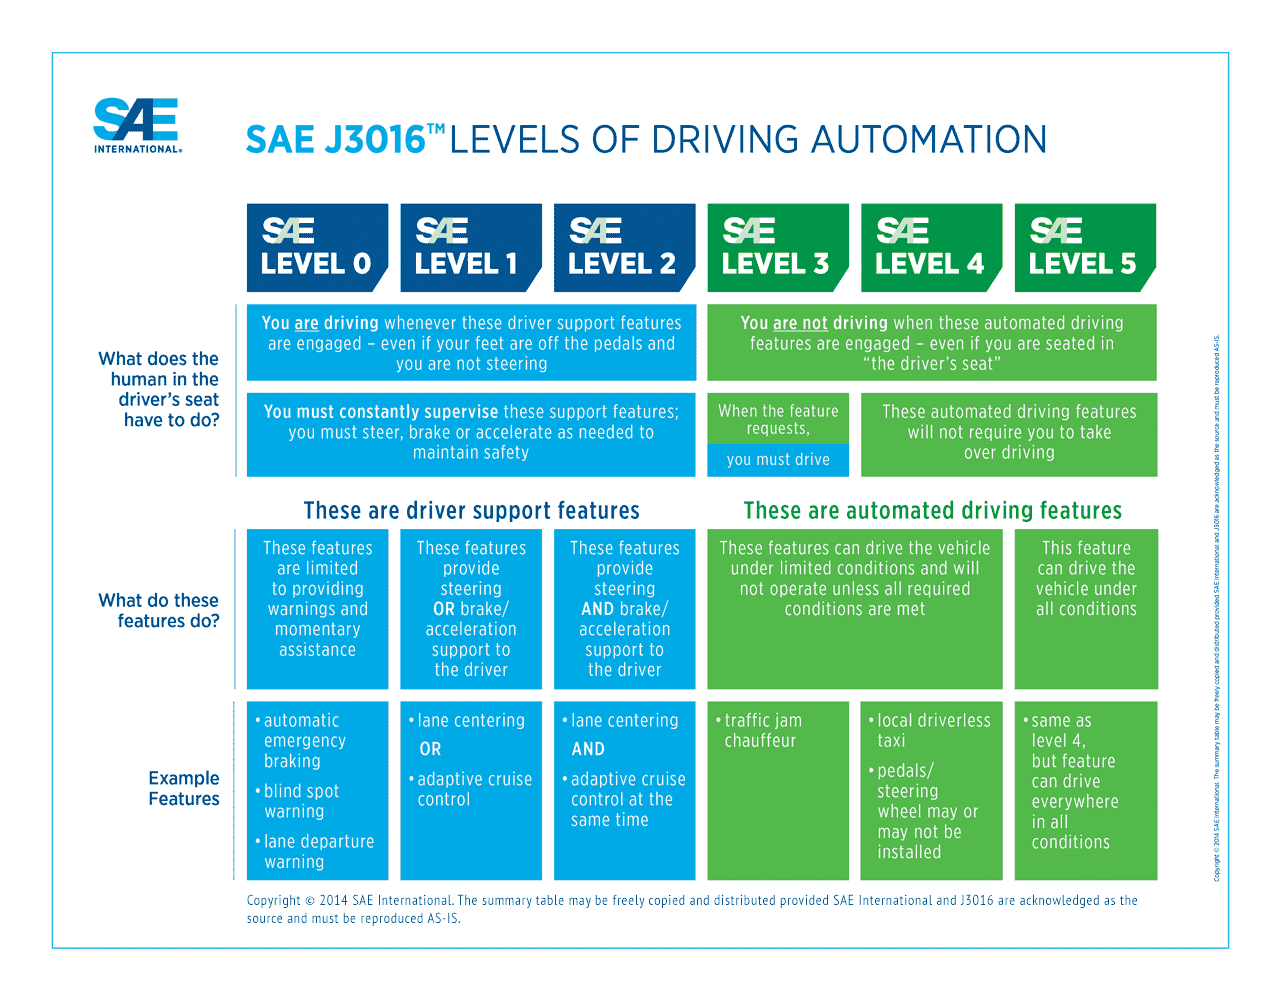
\includegraphics[width=0.9\linewidth]{image/adas_level} \caption{Levels of driving automation (Shuttleworth, 2019)}\label{fig:unnamed-chunk-38}
\end{figure}

\hypertarget{key-stakeholders-34}{%
\subsection*{Key stakeholders}\label{key-stakeholders-34}}
\addcontentsline{toc}{subsection}{Key stakeholders}

\begin{itemize}
\tightlist
\item
  \textbf{Affected}: Car Drivers, Traffic participants, Insurers
\item
  \textbf{Responsible}: Car manufacturers
\end{itemize}

\hypertarget{current-state-of-art-in-research-34}{%
\subsection*{Current state of art in research}\label{current-state-of-art-in-research-34}}
\addcontentsline{toc}{subsection}{Current state of art in research}

Important strands of research regarding ADAS include \emph{(1)} technical improvement of efficiency, reliability and functionality of the system (e.g.~Storsæter et al., 2021; Capodieci et al., 2021; Tsai et al., 2021; Tian e al., 2021) and \emph{(2)} human aspect of the system use which looks at \emph{(a)} how to convey information about the capabilities as well as limitations of ADAS in order not to offset the advantages stemming from its employment in the vehicles and \emph{(b)} how the performance of the system in a specific context influences the driver's perception of the system.

This human-centred research focuses mainly on exploration of the awareness of drivers and vehicle buyers to encourage safe use of ADAS. It is crucial because a study by Harms et al.~(2020) showed that many business drivers were unaware of which ADAS their car was equipped with and the reported ownership of ADAS (as measured in self-reported questionnaire) did not match the actual ownership of ADAS, demonstrating the lack of knowledge among drivers. This, in turn, may result in low social acceptance and usability of these safety systems in practice. Further, a Dutch study showed that sellers and consumers lack centralised database of ADAS functions. Consequently, many consumers do not receive information about ADAS and/or cannot try them out at the sale point. It was also showed that independent car dealers struggle to obtain information about ADAS (Boelhouwer et al., 2020).

Moreover, with respect to impact of context on driver's perception of ADAS, the study by Orlovska (2020) showed that the driving context strongly influences ADAS usage based on its performance which consequently may have impact on driver's trust and propensity to use the system in the long-run. Furthermore, it was showed that decisions of the driver regarding the engagement of ADAS while driving are affected by current driving conditions at the time when the decision is made. These results show an interconnection between the context, driver and the ADAS system usage. Beyond, the main findings of literature on driver distraction and behavioural adaptation in the context of ADAS are that \emph{(1)} drivers increase their engagement in secondary tasks (as well as their performance in these tasks) when driving with ADAS, \emph{(2)} drivers' situational awareness is lower when using ADAS \emph{(3)} the use of ADAS results in longer reaction times, more lane keeping variability and decrease in mental workload. Moreover, it is claimed that when drivers are exposed to automation systems which exceed their expectations, they tend to trust the systems and may not be aware of its limitations. The over-confidence in ADAS, in turn, increases the risk of collision (Hungund et al., 2021).

Beyond, a particular case of ADAS research focuses on older drivers (Chalkiadakis et al., 2020) and looks at the potential of ADAS in alleviating typical impairments such as reduced peripheral vision, night-time visual problems, longer reaction times, misjudgements of distance and speed and selective attention. As a result, the following functionalities are relevant:

\begin{itemize}
\tightlist
\item
  Blind spot detection
\item
  Obstacle detection system
\item
  Collision warning system
\item
  Navigation/Route guidance
\item
  Lane-keeping system
\item
  Night vision system
\item
  In-vehicle signage system
\item
  Driver condition monitoring system
\item
  Congestion and weather warning
\end{itemize}

Furthermore, study by Zahabi et al.~(2021) showed that demonstration-based training for ADAS is more effective for older male while video-based one for older female.

\hypertarget{current-state-of-art-in-practice-34}{%
\subsection*{Current state of art in practice}\label{current-state-of-art-in-practice-34}}
\addcontentsline{toc}{subsection}{Current state of art in practice}

It is generally claimed that, in practice, we have currently reached level 2 automation (in SAE classification, see table above) where vehicle can steer and accelerate, however it still does not drive itself and the driver is fully responsible for the car. A recent survey conducted by \href{https://www.rolandberger.com/en/Insights/Publications/Advanced-Driver-Assistance-Systems-A-ubiquitous-technology-for-the-future-of.html}{Roland Berger} on 80 global producers, automotive experts, industry suppliers and three thousand drivers shows that 85\% of vehicles produced globally in 2025 will be equipped with at least level 1 driving automation features. At the same time, it is not anticipated that level 4 or 5 automation will be present in more than 1\% of the vehicles by then (Shirokinskiy et al., 2021).

Moreover, current pandemic has been showed to slow down the overall development in ADAS systems, reaching in some cases -17\% (Shirokinskiy et al., 2021). Further challenge faced by the industry is lack of standardized nomenclature for ADAS features which, on one hand makes the tracking of these features difficult, on the other hand, it creates barriers for understanding of functionalities among drivers. For example, the adaptive cruise control (ACC) feature is known as Adaptive Cruise Control in Fiat, Ford, Volkswagen and Peugeot vehicles, as Intelligent Cruise Control in Citroen and BMW and DISTRONIC in Mercedes (Helman \& Carsten, 2019). In May 2020, SAE issued a \href{https://www.repairerdrivennews.com/2020/05/15/sae-international-endorses-generic-adas-terminology-recommendations/}{generic ADAS terminology recommendations} to tackle standardization issues (Huetter, 2020).

\hypertarget{relevant-initiatives-in-austria-34}{%
\subsection*{Relevant initiatives in Austria}\label{relevant-initiatives-in-austria-34}}
\addcontentsline{toc}{subsection}{Relevant initiatives in Austria}

\begin{itemize}
\tightlist
\item
  \href{https://www.alp-lab.at/}{Alp-lab}
\item
  \href{https://www.smartmicro.com/press-media/detail/smartmicro-sensors-deployed-in-austria}{Smartmicro.com}
\end{itemize}

\hypertarget{impacts-with-respect-to-sustainable-development-goals-sdgs-34}{%
\subsection*{Impacts with respect to Sustainable Development Goals (SDGs)}\label{impacts-with-respect-to-sustainable-development-goals-sdgs-34}}
\addcontentsline{toc}{subsection}{Impacts with respect to Sustainable Development Goals (SDGs)}

\begin{longtable}[]{@{}
  >{\centering\arraybackslash}p{(\columnwidth - 8\tabcolsep) * \real{0.2029}}
  >{\centering\arraybackslash}p{(\columnwidth - 8\tabcolsep) * \real{0.1884}}
  >{\centering\arraybackslash}p{(\columnwidth - 8\tabcolsep) * \real{0.2029}}
  >{\centering\arraybackslash}p{(\columnwidth - 8\tabcolsep) * \real{0.2029}}
  >{\centering\arraybackslash}p{(\columnwidth - 8\tabcolsep) * \real{0.2029}}@{}}
\toprule()
\begin{minipage}[b]{\linewidth}\centering
Impact level
\end{minipage} & \begin{minipage}[b]{\linewidth}\centering
Indicator
\end{minipage} & \begin{minipage}[b]{\linewidth}\centering
Impact direction
\end{minipage} & \begin{minipage}[b]{\linewidth}\centering
Goal description and number
\end{minipage} & \begin{minipage}[b]{\linewidth}\centering
Source
\end{minipage} \\
\midrule()
\endhead
Individual & ADAS alleviates impact of aging-related impairments & \textbf{+} & Health \& Wellbeing (\emph{3}) & Chalkiadakis et al., 2020 \\
Individual & Facilitates mobility for elderly drivers & \textbf{+} & Equality (\emph{5,10}) & Chalkiadakis et al., 2020 \\
Systemic & Increases driving comfort but scarce unambiguous evidence of impact on safety & \textbf{\textasciitilde{}} & Health \& Wellbeing (\emph{3}) & Sullivan et al., 2016 \\
Systemic & Global trends in ADAS R\&D & \textbf{+} & Innovation \& Infrastructure (\emph{9}) & Yochman, 2020 \\
\bottomrule()
\end{longtable}

\hypertarget{technology-and-societal-readiness-level-34}{%
\subsection*{Technology and societal readiness level}\label{technology-and-societal-readiness-level-34}}
\addcontentsline{toc}{subsection}{Technology and societal readiness level}

\begin{longtable}[]{@{}cc@{}}
\toprule()
TRL & SRL \\
\midrule()
\endhead
7-9 & 6-8 \\
\bottomrule()
\end{longtable}

\hypertarget{open-questions-32}{%
\subsection*{Open questions}\label{open-questions-32}}
\addcontentsline{toc}{subsection}{Open questions}

\begin{enumerate}
\def\labelenumi{\arabic{enumi}.}
\tightlist
\item
  How can ADAS nomenclature standardization be encouraged and achieved?
\item
  How to incorporate the impact of behavioural adaptation into ADAS design to a larger degree?
\end{enumerate}

\hypertarget{further-links-29}{%
\subsection{Further links}\label{further-links-29}}

\begin{itemize}
\tightlist
\item
  \href{https://ec.europa.eu/transport/road_safety/sites/default/files/pdf/ersosynthesis2018-adas.pdf}{ec.europa.eu}
\item
  \href{https://aaafoundation.org/wp-content/uploads/2017/12/BehavioralAdaptationADAS.pdf}{aaafoundation.org}
\end{itemize}

\hypertarget{references-34}{%
\subsection*{References}\label{references-34}}
\addcontentsline{toc}{subsection}{References}

\begin{itemize}
\tightlist
\item
  Boelhouwer, A., Van den Beukel, A. P., Van der Voort, M. C., Hottentot, C., De Wit, R. Q., \& Martens, M. H. (2020). How are car buyers and car sellers currently informed about ADAS? An investigation among drivers and car sellers in the Netherlands. Transportation Research Interdisciplinary Perspectives, 4, 100103.
\item
  Capodieci, N., Cavicchioli, R., Muzzini, F., \& Montagna, L. (2021). Improving emergency response in the era of ADAS vehicles in the Smart City. ICT Express.
\item
  Chalkiadakis, C., Mitsakis, E., \& Tzanis, D. (2020, September). Requirements for the development and implementation of ADAS and C-ITS services for older drivers. In 2020 IEEE 23rd International Conference on Intelligent Transportation Systems (ITSC) (pp.~1-6). IEEE.
\item
  Harms, I. M., Bingen, L., \& Steffens, J. (2020). Addressing the awareness gap: A combined survey and vehicle registration analysis to assess car owners' usage of ADAS in fleets. Transportation Research Part A: Policy and Practice, 134, 65-77.
\item
  Helman, S. \& Carsten, O. (2019) What does my car do? Available at: \url{https://www.pacts.org.uk/wp-content/uploads/What-does-my-car-do-2.1_.pdf} {[}Accessed: 31 May 2021{]}.
\item
  Huetter, J. (2020) SAE International endorses generic ADAS terminology recommendations. Available at \textless{} \url{https://www.repairerdrivennews.com/2020/05/15/sae-international-endorses-generic-adas-terminology-recommendations/}\textgreater{} Accessed: 31/05/2021
\item
  Hungund, A. P., Pai, G., \& Pradhan, A. K. (2021). Systematic Review of Research on Driver Distraction in the Context of Advanced Driver Assistance Systems. Transportation Research Record, 03611981211004129.
\item
  Orlovska, J., Novakazi, F., Lars-Ola, B., Karlsson, M., Wickman, C., \& Söderberg, R. (2020). Effects of the driving context on the usage of Automated Driver Assistance Systems (ADAS)-Naturalistic Driving Study for ADAS evaluation. Transportation research interdisciplinary perspectives, 4, 100093.
\item
  Samsara.com (2020). Advanced Driver Assistance Systems (ADAS) for Commercial Fleets. Available at:\textless{} \url{https://www.samsara.com/guides/adas}\textgreater{} {[}Accessed: 28 April 2021{]}.
\item
  Shirokinskiy, K., Bernhart, W. and Keese, S., 2021. Advanced Driver-Assistance Systems: A ubiquitous technology for the future of vehicles. Roland Berger. Available at: \url{https://www.rolandberger.com/en/Insights/Publications/Advanced-Driver-Assistance-Systems-A-ubiquitous-technology-for-the-future-of.html} {[}Accessed: 31 May 2021{]}.
\item
  Shuttleworth, J. (2019). SAE Standards News: J3016 automated-driving graphic update. Available at: \url{https://www.sae.org/news/2019/01/sae-updates-j3016-automated-driving-graphic} {[}Accessed: 28 April 2021{]}.
\item
  Storsæter, A. D., Pitera, K., \& McCormack, E. (2021). Using ADAS to Future-Proof Roads---Comparison of Fog Line Detection from an In-Vehicle Camera and Mobile Retroreflectometer. Sensors, 21(5), 1737.
\item
  Sullivan, J. M., Flannagan, M. J., Pradhan, A. K., \& Bao, S. (2016). Literature review of behavioral adaptations to advanced driver assistance systems.
\item
  Tian, J., Liu, S., Zhong, X., \& Zeng, J. (2021). LSD-based adaptive lane detection and tracking for ADAS in structured road environment. Soft Computing, 25(7), 5709-5722.
\item
  Tsai, W. C., Lai, J. S., Chen, K. C., M Shivanna, V., \& Guo, J. I. (2021). A lightweight motional object behavior prediction system harnessing deep learning technology for embedded adas applications. Electronics, 10(6), 692.
\item
  Yochman, F. (2020) Top automakers with highest ADAS and autonomous vehicles R\&D spending. Available at: \textless{} \url{https://m14intelligence.com/public/index.php/blog/34}\textgreater{} {[}Accessed: 31 April 2021{]}.
\item
  Zahabi, M., Razak, A. M. A., Mehta, R. K., \& Manser, M. (2021). Effect of advanced driver-assistance system trainings on driver workload, knowledge, and trust. Transportation research part F: traffic psychology and behaviour, 76, 309-320.
\end{itemize}

\hypertarget{parking_assistance}{%
\section{Parking assistance system}\label{parking_assistance}}

\hypertarget{definition-35}{%
\subsection*{Definition}\label{definition-35}}
\addcontentsline{toc}{subsection}{Definition}

Nowadays, parking a car becomes an increasingly mundane task due to the growing size of the vehicles which consequently reduces visibility to the rear and front. Moreover, the number of vehicles on the road continues to increase which makes finding parking spaces more difficult. To overcome this challenge, efficient and advanced parking techniques are needed, such as finding the right parking space and parking cars efficiently (Khalid et al., 2021).
While in the 1990s parking assistance systems were not considered necessary, systems that support the parking process are now standard in new vehicles and have a high acceptance rate. While parking assistance systems of the first generations were mainly informative systems, today these systems help to find a suitable parking space and support the steering during the parking manoeuvre. Future systems will become even more autonomous, up to a point where they will find their parking space without human intervention (Automated Valet Parking) (Gotzig, 2016).

With respect to safety issues, parking assistance systems can reduce insurance claims that occur during parking manoeuvres by 30\% (ADAC, 2020). They also provide a useful application in the form of emergency brake assistant that prevents accidents with other road users when reversing (ADAC, 2019).

Modern Parking assistants work with two sensor concepts: ultrasonic sensors for the close range at the rear (often already installed as ``parking beepers'') and radar sensors with a longer range at the side in the bumper (ADAC, 2019). Additionally, there are also new releases with 360° view around the car (Land Rover, n.d.; Mercedes-Benz, n.d.). However, there are no tests for this at the moment.

\hypertarget{key-stakeholders-35}{%
\subsection*{Key stakeholders}\label{key-stakeholders-35}}
\addcontentsline{toc}{subsection}{Key stakeholders}

\begin{itemize}
\tightlist
\item
  \textbf{Affected}: Car Drivers, Traffic participants, Insurers
\item
  \textbf{Responsible}: Car manufacturers
\end{itemize}

\hypertarget{current-state-of-art-in-research-35}{%
\subsection*{Current state of art in research}\label{current-state-of-art-in-research-35}}
\addcontentsline{toc}{subsection}{Current state of art in research}

The research on on-board parking features is almost entirely owned by the car manufacturers. Research tends to focus on larger-scale issues such as car parking location tracking, space booking systems using IoT and congestion caused by \emph{parking cruises}.
Additionally, tests are carried out on the merger between emergency brake assistant and parking assistant to overcome the difficulties with obstacles detection and reduce the collision rates in this specific situation. The ADAC tested the AEB (Autonomous Emergency Braking) systems from Mercedes, Volvo, BMW, Seat and Skoda in three test scenarios: \emph{(1)} a pedestrian dummy stands behind a car or walks past, \emph{(2)} a car parks in the direction of travel and \emph{(3)} cyclists as well as cars drive past crosswise.
BMW was the best at reacting to all situations with radar and ultrasound - with some drop-outs, especially with moving pedestrians or cross-traffic. The Mercedes, on the other hand, only used its side radar sensors for reverse braking and thus did not recognise stationary vehicles at all. The VW system from Skoda and Seat had radar and ultrasound, but moving pedestrians were only detected randomly or not at all.
Overall, these tests showed that the automatic braking parking assistants have a lot of potential, but are far from optimal. Even the system of the front-runners does not yet work 100\% reliably. Even the low-cost ultrasonic sensors, however, can be very effective and even prevent pedestrian collisions, as the BMW showed in the test. Therefore, it is crucial that manufacturers equip their vehicles with an effective AEB system as a standard. The necessary technology is already available in most passenger cars where the rear ultrasonic sensors would need to be linked to the braking function (ADAC, 2019).
The greatest difficulties are encountered in pedestrian detection, in the scenarios in which the risk of personal injury is potentially the highest. Some of the tested vehicles recognised the dangerous situation too late or not at all.

\hypertarget{current-state-of-art-in-practice-35}{%
\subsection*{Current state of art in practice}\label{current-state-of-art-in-practice-35}}
\addcontentsline{toc}{subsection}{Current state of art in practice}

Nearly 50\% of the cars in Germany are now equipped with parking assistance. Nonetheless, the results of a study by HUK-Coburg, Germany's largest motor insurer with eleven million insured cars, show that the number of fender-benders has not decreased and the damage costs have even risen slightly. The reason for this is the damage to the expensive Park Distance Control (PDC) sensor embedded in the bumper when vehicle collides with an obstacle while parking (Focus Online, 2017).
In 2017, 570 accidents with personal injury occurred in Austria when reversing with passenger cars. There were no fatalities, but around 290 people were injured, 60 of them seriously. In addition, there is a large amount of property damage due to obstacles being overlooked (ÖAMTC, 2019).
According to different sources, between 23\% and 46\% of the cars in Germany are equipped with an on-board parking assistant (Focus Online, 2017). In contrast, only 13\% of the vehicles are equipped with an emergency brake assistant that automatically brakes in the event of an imminent collision with the vehicle in front or even detects pedestrians and cyclists. Further, a survey conducted on 1000 respondents by German Road Safety Council showed that 85\% of the sample found the emergency brake assistant as highly useful and 65\% considered parking assistant highly beneficial (Handelsblatt, 2016).
Currently, the most advanced technology with respect to parking assistance is offered by Tesla S, where the system is fully autonomous and allows the car to drive itself out of a tight space without the driver's intervention. But it is expected that the technology will be available from other manufacturers too and will improve rapidly in the coming years. One reason for this is that parking assistants with brake intervention will become part of the European vehicle test programme \emph{Euro NCAP} from 2020. In the past, it has been shown that the inclusion of active and passive passenger car safety systems in this programme quickly increases the rate at which vehicles are equipped (ÖAMTC, 2019).

\hypertarget{relevant-initiatives-in-austria-35}{%
\subsection*{Relevant initiatives in Austria}\label{relevant-initiatives-in-austria-35}}
\addcontentsline{toc}{subsection}{Relevant initiatives in Austria}

\begin{itemize}
\tightlist
\item
  \href{https://www.oeamtc.at/tests/assistenzsystemtest/fuenf-parkassistenten-mit-notbremssystem-im-test-31717317}{oeamtc.at}
\end{itemize}

\hypertarget{impacts-with-respect-to-sustainable-development-goals-sdgs-35}{%
\subsection*{Impacts with respect to Sustainable Development Goals (SDGs)}\label{impacts-with-respect-to-sustainable-development-goals-sdgs-35}}
\addcontentsline{toc}{subsection}{Impacts with respect to Sustainable Development Goals (SDGs)}

\begin{longtable}[]{@{}
  >{\centering\arraybackslash}p{(\columnwidth - 8\tabcolsep) * \real{0.2029}}
  >{\centering\arraybackslash}p{(\columnwidth - 8\tabcolsep) * \real{0.1884}}
  >{\centering\arraybackslash}p{(\columnwidth - 8\tabcolsep) * \real{0.2029}}
  >{\centering\arraybackslash}p{(\columnwidth - 8\tabcolsep) * \real{0.2029}}
  >{\centering\arraybackslash}p{(\columnwidth - 8\tabcolsep) * \real{0.2029}}@{}}
\toprule()
\begin{minipage}[b]{\linewidth}\centering
Impact level
\end{minipage} & \begin{minipage}[b]{\linewidth}\centering
Indicator
\end{minipage} & \begin{minipage}[b]{\linewidth}\centering
Impact direction
\end{minipage} & \begin{minipage}[b]{\linewidth}\centering
Goal description and number
\end{minipage} & \begin{minipage}[b]{\linewidth}\centering
Source
\end{minipage} \\
\midrule()
\endhead
Individual & Road accidents when parking reduced & \textbf{+} & Health \& Wellbeing (\emph{3}) & ADAC, 2019 \\
Individual & Higher costs in case of collision & \textbf{-} & Sustainable economic development (\emph{8,11}) & Focus Online, 2017 \\
Systemic & New designs tested & \textbf{+} & Innovation \& Infrastructure (\emph{9}) & Euro NCAP, 2021 \\
\bottomrule()
\end{longtable}

\hypertarget{technology-and-societal-readiness-level-35}{%
\subsection*{Technology and societal readiness level}\label{technology-and-societal-readiness-level-35}}
\addcontentsline{toc}{subsection}{Technology and societal readiness level}

\begin{longtable}[]{@{}cc@{}}
\toprule()
TRL & SRL \\
\midrule()
\endhead
8-9 & 8-9 \\
\bottomrule()
\end{longtable}

\hypertarget{open-questions-33}{%
\subsection*{Open questions}\label{open-questions-33}}
\addcontentsline{toc}{subsection}{Open questions}

\begin{enumerate}
\def\labelenumi{\arabic{enumi}.}
\tightlist
\item
  How can acceptance and usability rates be increased in drivers especially in elderly group?
\item
  What are the legal implications for the use of assisted parking for both drivers and car manufacturers?
\end{enumerate}

\hypertarget{references-35}{%
\subsection*{References}\label{references-35}}
\addcontentsline{toc}{subsection}{References}

\begin{itemize}
\tightlist
\item
  ADAC. (2019, May 14). Parkassistenten im Test: Noch nicht gut genug. \url{https://presse.adac.de/meldungen/adac-ev/tests/parkassistent.html}
\item
  ADAC. (2020, January 9). Fahrerassistenzsysteme im Überblick \textbar{} ADAC. \url{https://www.adac.de/rund-ums-fahrzeug/ausstattung-technik-zubehoer/assistenzsysteme/fahrerassistenzsysteme/}
\item
  Euro NCAP. (2021). \url{http://www.euroncap.com} (Accessed: 26 February 2021)
\item
  Focus Online. (2017, April 27). Einparkhilfen bringen nichts - sondern verursachen mehr Schaden - FOCUS Online. \url{https://www.focus.de/auto/news/untersuchung-der-huk-coburg-studie-einparkhilfe-hilft-nicht-sie-versucht-eher-mehr-schaden_id_7035248.html}
\item
  Gotzig, H. (2016). Parking Assistance. In H. Winner, S. Hakuli, F. Lotz, \& C. Singer (Eds.), Handbook of Driver Assistance Systems: Basic Information, Components and Systems for Active Safety and Comfort (pp.~1077--1092). Springer International Publishing. \url{https://doi.org/10.1007/978-3-319-12352-3_45}
\item
  Handelsblatt. (2016, April 8). Umfrage zu Assistenzsystemen\,: Einparkassistent nützlich, Notbremsassistent nützlicher. \url{https://www.handelsblatt.com/auto/nachrichten/umfrage-zu-assistenzsystemen-einparkassistent-nuetzlich-notbremsassistent-nuetzlicher/13404708.html?ticket=ST-4955434-naHBLAxI66h66nbvrBXF-ap1}
\item
  Khalid, M., Wang, K., Aslam, N., Cao, Y., Ahmad, N., \& Khan, M. K. (2021). From smart parking towards autonomous valet parking: A survey, challenges and future Works. Journal of Network and Computer Applications, 175, 102935. \url{https://doi.org/https://doi.org/10.1016/j.jnca.2020.102935}
\item
  Land Rover. (n.d.). Parking Assistance \textbar{} InControl \textbar{} Land Rover UK. Available at: \url{https://www.landrover.co.uk/incontrol/driver-safety-and-assistance/parking-assistance.html} {[}Accessed: 25 February 2021{]}
\item
  Margreiter, M., Mayer, P., Alpas, M., \& Vlahogianni, E. (2017). Driver's Willingness to Use Parking Assistance Tools and their Expectations: A Case Study for the Cities of Munich and Athens. In 8th International Congress on Transportation Research.
\item
  Mercedes-Benz. (n.d.). Mercedes-Benz X-Klasse: Park-Paket mit 360°-Kamera. Available at: \url{https://www.mercedes-benz.at/passengercars/mercedes-benz-cars/models/x-class/x-class-pickup/facts-and-lines/equipment-packages/360-camera.html} {[}Accessed: 25 February 2021{]}
\item
  Tsugawa, S. (2006). Trends and issues in safe driver assistance systems: Driver acceptance and assistance for elderly drivers. IATSS research, 30(2), 6-18.
\item
  ÖAMTC. (2019, May 14). ÖAMTC: Fünf Parkassistenten mit Notbremssystem im Test (+ Fotos, + Grafik) \textbar{} ÖAMTC, 14.05.2019. \url{https://www.ots.at/presseaussendung/OTS_20190514_OTS0021/oeamtc-fuenf-parkassistenten-mit-notbremssystem-im-test-fotos-grafik}
\end{itemize}

\hypertarget{lane_keeping}{%
\section{Lane keeping assist system}\label{lane_keeping}}

\hypertarget{synonyms-31}{%
\subsection*{Synonyms}\label{synonyms-31}}
\addcontentsline{toc}{subsection}{Synonyms}

\emph{Lane Keeping Assist System (LKAS), Lane Keeping Assist (LKA)}

\hypertarget{definition-36}{%
\subsection*{Definition}\label{definition-36}}
\addcontentsline{toc}{subsection}{Definition}

Lane keeping assist monitors road markings, typically using a camera located behind the windscreen to keep the car within its driving lane and as a result reduce the burden of the driver. There are different systems currently available and they are not the same (Autonationdrive, 2019):

\begin{itemize}
\tightlist
\item
  \textbf{Lane Departure Warning (LDW)}: Audible or visual warnings signal to the driver that their vehicle is approaching or may be crossing the lane markings.
\item
  \textbf{Road Departure Assist (RDA)}: An automatic steering system, which may also include an automatic braking system, keeps the vehicle on the roadway itself.
\item
  \textbf{Lane Keeping Assist (LKA)}: An automatic steering system, which may also include an automatic braking system, keeps the vehicle within its lane.
\item
  \textbf{Lane Centering Assist (LCA)}: An automatic steering system, which may also include an automatic braking system, to keep the vehicle in the center of the lane.
\end{itemize}

The main difference between them is that LDW informs the driver in case of crossing the road marking through different sensory cues such as tactile, visual or audio, the LKAS helps the driver to stay within the lane through the adjustments to steering wheel movements depending on the distance from the lane marking on either side. The systems can use reactive or proactive process, where the vehicle is reactively put back on track while it begins to leave the lane or proactively kept in the centre of the lane, respectively. It is usually activated by the driver and works at speed between 65 km/h and 180 km/h and radius of 230 m. Hence, it is the most suitable for highways and motorways but less so for urban or country roads. Even though the LKAS is activated, the driver remains responsible for controlling the vehicle. Consequently, LKAS continuously checks the steering movements applied by the driver and if he has his/her hands on the steering wheel. In case, the system detects that driver is not actively steering, it produces the waring and deactivates. This is to ensure that the driver remains in control throughout. Moreover, the driver can overrule the LKAS at any time. For example, LKAS deactivates automatically when braking and deliberate lane charge activated via the use of indicators (blinkers) (VDA, 2021).

\hypertarget{key-stakeholders-36}{%
\subsection*{Key stakeholders}\label{key-stakeholders-36}}
\addcontentsline{toc}{subsection}{Key stakeholders}

\begin{itemize}
\tightlist
\item
  \textbf{Affected}: General public, Drivers, Road infrastructure companies, Insurers
\item
  \textbf{Responsible}: Car manufacturers, Transport agencies, National governments and International bodies (e.g.~EU or \href{https://unece.org/fileadmin/DAM/trans/main/wp29/wp29regs/2018/R079r4e.pdf}{UNECE})
\end{itemize}

\hypertarget{current-state-of-art-in-research-36}{%
\subsection*{Current state of art in research}\label{current-state-of-art-in-research-36}}
\addcontentsline{toc}{subsection}{Current state of art in research}

Current research explores new approaches to the development of lane keeping assistance such as the use of Global Navigation Satellite System (Tominaga et al., 2020), deep learning (Wang et al., 2020) or neural network techniques (Yusuf et al., 2020). Beyond, it aims at the validation and improvement of LKAS by looking at the impact of system design (Lee et al., 2018) and different road conditions on the overall quality performance of lane keeping assistance (Romano et al., 2020). Further, a number of studies explored the potential of including driver's characteristics to develop of personalised lane keeping assist.
Further, study by Weaver \& Gonzalez (2020) focused on the influence of LKAS on drivers' behaviour and acceptance level of LKAS technology. It not only confirmed existing findings that more experience and familiarity with the system increases acceptance rate and trust, but it also showed a positive response from individuals who had no previous experience in using LKAS.

\hypertarget{current-state-of-art-in-practice-36}{%
\subsection*{Current state of art in practice}\label{current-state-of-art-in-practice-36}}
\addcontentsline{toc}{subsection}{Current state of art in practice}

In Europe the main existing legal basis for lane keeping systems that regulate its use is \href{https://op.europa.eu/en/publication-detail/-/publication/bfd5eba8-2058-11ea-95ab-01aa75ed71a1/language-en}{Regulation (EU) 2019/2144}. Hence, many car manufacturers nowadays offer cars featured with lane keeping assist which together with other system such as automatic cruise control or \protect\hyperlink{distance_keeping}{distance keeping} already provide a high level of automation. Some of many producers offering LKAS are \href{https://www.bosch-mobility-solutions.com/en/products-and-services/passenger-cars-and-light-commercial-vehicles/driver-assistance-systems/lane-keeping-assist/}{BOSCH}, \href{https://www.hondainfocenter.com/2021/CR-V/Feature-Guide/Interior-Features/Lane-Keeping-Assist-System-LKAS/}{Honda}, \href{https://www.tesla.com/de_DE/blog/more-advanced-safety-tesla-owners?redirect=no}{Tesla} or \href{https://owner.ford.com/support/how-tos/safety/driver-assist-technology/driving/how-to-use-lane-keeping-system.html}{Ford}.

In terms of the accident prevention, lane keeping assist has a huge potential to increase road safety where National Highway Traffic Safety Administration (NHTSA) data from 2011 show that 53\% of road fatalities result from a roadway departure (Automotive World, 2013). In fact, real world data from Sweden shows that crashes involving out-of-lane drift were reduced by 40\% for cars with Electronic Stability Control (ESC) as opposed to 29\% for cars without it (Sternlung, 2018).

The major disadvantage of lane keeping systems is the fact that it relies on a visual detection of painted road marking in order to work effectively therefore any condition deterioration such as night-time or rain have a significant impact on the system performance (Tchir, 2019).

\hypertarget{relevant-initiatives-in-austria-36}{%
\subsection*{Relevant initiatives in Austria}\label{relevant-initiatives-in-austria-36}}
\addcontentsline{toc}{subsection}{Relevant initiatives in Austria}

\begin{itemize}
\tightlist
\item
  \href{https://www.ertrac.org/uploads/images/ERTRAC2019-Connected-Automated-Driving-Roadmap\%20-2019-04-04.pdf}{ertrac.org}
\end{itemize}

\hypertarget{impacts-with-respect-to-sustainable-development-goals-sdgs-36}{%
\subsection*{Impacts with respect to Sustainable Development Goals (SDGs)}\label{impacts-with-respect-to-sustainable-development-goals-sdgs-36}}
\addcontentsline{toc}{subsection}{Impacts with respect to Sustainable Development Goals (SDGs)}

\begin{longtable}[]{@{}
  >{\centering\arraybackslash}p{(\columnwidth - 8\tabcolsep) * \real{0.2029}}
  >{\centering\arraybackslash}p{(\columnwidth - 8\tabcolsep) * \real{0.1884}}
  >{\centering\arraybackslash}p{(\columnwidth - 8\tabcolsep) * \real{0.2029}}
  >{\centering\arraybackslash}p{(\columnwidth - 8\tabcolsep) * \real{0.2029}}
  >{\centering\arraybackslash}p{(\columnwidth - 8\tabcolsep) * \real{0.2029}}@{}}
\toprule()
\begin{minipage}[b]{\linewidth}\centering
Impact level
\end{minipage} & \begin{minipage}[b]{\linewidth}\centering
Indicator
\end{minipage} & \begin{minipage}[b]{\linewidth}\centering
Impact direction
\end{minipage} & \begin{minipage}[b]{\linewidth}\centering
Goal description and number
\end{minipage} & \begin{minipage}[b]{\linewidth}\centering
Source
\end{minipage} \\
\midrule()
\endhead
Individual & Accident risk reduced; low performance in suboptimal road conditions & \textbf{\textasciitilde{}} & Health \& Wellbeing (\emph{3}) & Sterlund, 2018; Tchir, 2019 \\
Systemic & Systems are continuously improved & \textbf{+} & Innovation \& Infrastructure (\emph{9}) & Lawrence \& Kareta, 2020 \\
\bottomrule()
\end{longtable}

\hypertarget{technology-and-societal-readiness-level-36}{%
\subsection*{Technology and societal readiness level}\label{technology-and-societal-readiness-level-36}}
\addcontentsline{toc}{subsection}{Technology and societal readiness level}

\begin{longtable}[]{@{}cc@{}}
\toprule()
TRL & SRL \\
\midrule()
\endhead
5-7 & 5-7 \\
\bottomrule()
\end{longtable}

\hypertarget{open-questions-34}{%
\subsection*{Open questions}\label{open-questions-34}}
\addcontentsline{toc}{subsection}{Open questions}

\begin{enumerate}
\def\labelenumi{\arabic{enumi}.}
\tightlist
\item
  What are the implication of lane keeping systems for physical infrastructure (such as contrast and colour of painted lanes) and how these can be improved to enhance the effectiveness of lane keeping systems?
\item
  Cross-national standardisation of road markings is required to ensure equal safety levels.
\end{enumerate}

\hypertarget{further-links-30}{%
\subsection*{Further links}\label{further-links-30}}
\addcontentsline{toc}{subsection}{Further links}

\begin{itemize}
\tightlist
\item
  \href{https://www.mes-insights.com/automated-lane-keeping-systems-pave-the-autonomous-car-future-a-965712/}{mes-insights.com}
\end{itemize}

\hypertarget{references-36}{%
\subsection*{References}\label{references-36}}
\addcontentsline{toc}{subsection}{References}

\begin{itemize}
\tightlist
\item
  Automotive World (2013) Latest Lane Keeping Assist technology from TRW goes into production. Available at: \url{https://www.automotiveworld.com/news-releases/latest-lane-keeping-assist-technology-from-trw-goes-into-production/} {[}Accessed: 7 April 2021{]}.
\item
  Autonationdrive (2019). Best Cars with Lane Assist. Available at: \url{https://www.autonationdrive.com/research/best-cars-with-lane-assist.htm} {[}Accessed: 7 April 2021{]}
\item
  Lawrence, C. \& Kareta, N. (2020). Automated Lane Keeping Systems pave the autonomous car future. Available at: \textless{} \url{https://www.mes-insights.com/automated-lane-keeping-systems-pave-the-autonomous-car-future-a-965712/}\textgreater{} {[}Accessed: 7 April 2021{]}
\item
  Romano, R., Maggi, D., Hirose, T., Broadhead, Z., \& Carsten, O. (2020). Impact of lane keeping assist system camera misalignment on driver behavior. Journal of Intelligent Transportation Systems, 1-13.
\item
  Sternlund, S. (2018). The Safety Potential and Effectiveness of Lane Departure Warning Systems in Passenger Cars. Chalmers Tekniska Hogskola (Sweden).
\item
  Tchir, J. (2019). The limitations of lane-keeping assist. Available at: \url{https://www.theglobeandmail.com/drive/mobility/article-the-limitations-of-lane-keeping-assist/} {[}Accessed: 7 April 2021{]}
\item
  Vda.de. 2021. VDA. Available at: \url{https://www.vda.de/en/topics/safety-and-standards/lkas/lane-keeping-assist-systems.html} {[}Accessed: 30 March 2021{]}.
\item
  Wang, Q., Zhuang, W., Wang, L., \& Ju, F. (2020). Lane Keeping Assist for an Autonomous Vehicle Based on Deep Reinforcement Learning (No.~2020-01-0728). SAE Technical Paper.
\item
  Weaver, S., \& Gonzalez, T. (2020). To Alert or Assist: Comparing Effects of Different Lateral Support Systems on Lane-Keeping (No.~FHWA-HRT-20-068).
\item
  Yusuf, M. M., Karim, T., \& Saif, A. S. (2020, January). A robust method for lane detection under adverse weather and illumination conditions using convolutional neural network. In Proceedings of the International Conference on Computing Advancements (pp.~1-8).
\end{itemize}

\hypertarget{digital_maps}{%
\section{Digital maps}\label{digital_maps}}

\textbf{Updated: 10th January 2022}

\hypertarget{synonyms-32}{%
\subsection*{Synonyms}\label{synonyms-32}}
\addcontentsline{toc}{subsection}{Synonyms}

\emph{High definition maps (HD maps), High precision maps}

\hypertarget{definition-37}{%
\subsection*{Definition}\label{definition-37}}
\addcontentsline{toc}{subsection}{Definition}

Digital Maps are electronic maps that gather and integrate data from Global Positioning System (GPS), Light Detection and Ranging System (LiDAR), radars and vehicle sensor in order to increase safety of autonomous and driverless cars, through the implementation of Artificial Intelligence (AI) and Internet of Things (IoT) (Kulkarni, 2021). They are highly precise and detailed lane-level maps which have an ultimate goal to provide virtual assistance on the extreme high safety standards while travelling in AVs (Zang et al., 2018). In particular, they increase vehicle's sensors information for contextual environment analysis to help performing manoeuvres beyond vehicle's sensing range by providing very accurate vehicle positioning and orientation in map coordinates. The digital maps used in AVs are frequently called High Definition (HD) maps, which have extremely high (centimetre-level) accuracy and are designed to tackle one of the biggest problems of autonomous driving, the determination of the exact position of a vehicle in real-time (Haydin, 2020). Currently, the global digital map market is estimated to reach around 12.7\% of Compound Annual Growth Rate (CAGR) in 2023, following the increase in demand for autonomous vehicles (Kulkarni, 2021). Consequently, global development of driverless cars and digital maps brings the potential for further implementation and development of smart solutions in cities infrastructure.

\hypertarget{key-stakeholders-37}{%
\subsection*{Key stakeholders}\label{key-stakeholders-37}}
\addcontentsline{toc}{subsection}{Key stakeholders}

\begin{itemize}
\tightlist
\item
  \textbf{Affected}: Users of AVs, Drivers of conventional vehicles, Pedestrians, Cyclists
\item
  \textbf{Responsible}: National and local governments, Private developers of digital mapping systems, Automotive companies, Car manufacturers
\end{itemize}

\hypertarget{current-state-of-art-in-research-37}{%
\subsection*{Current state of art in research}\label{current-state-of-art-in-research-37}}
\addcontentsline{toc}{subsection}{Current state of art in research}

The main trend in research regarding digital maps for AV purposes includes the improvement in their accuracy (especially in dense urban areas) and development of approaches to update the changes in physical environment on the road.

For example, the research conducted by Jo et al.~(2018) proposes two methods of updating HD maps with recent changes in the physical features of the real world. The first option relies on implementing ground-mapping technology, which assesses all the roads in the database in terms of feature changes and then detects them. However, this technology is not only expensive but also it works on a limited area. Second method makes use of perception and localization functions of driverless vehicles, through the created algorithm called Simultaneous Localization and Map Change Update (SLAMCU). Consequently, the update of data can be performed in many vehicles at the same time, which is a considerable advantage of this method. Additionally, there is no extra software, which makes this method much cheaper in comparison to the first one.

Further, Hartmann et al.~(2018) focuses on the improvement of the accuracy of digital maps, if they were to be used more broadly. The online verification approach is proposed, which detects changes in front of the car, based on the large databases and sensors. The database collects information about the road geometry and speed limits in the standard interface Advanced Driver Assistance Systems Interface Specifications (ADASIS). This approach provides higher accuracy (96.64\%) in comparison to the other systems. The authors concluded that there is needed further research to fully examine possibilities and function of this system.

Moreover, Arman \& Tampère (2021) investigate the creation of routable digital maps based on floating car data (trajectory data). The required data is easy and inexpensive to collect. The results show that this low-cost method can produce accurate, routable lane-level digital maps that can be used as a basis for analysing longitudinal and lateral driving behaviour, especially drivers' lane-changing manoeuvres. The proposed algorithm can determine the intersections, centreline, and lanes in a highway network. A robustness analysis of this method shows that 500-550 trajectories are sufficient to produce reliable routable digital maps (RDMs) at the lane level. The algorithm provides a way to make the fusion of data from different sources, including trajectory data collected by smartphones (cheap and large trajectory data), more accurate and to estimate traffic conditions more accurately. Despite important achievements, there is still room for improvement and expansion. To adapt to the urban road network, it is essential to separate GPS tracks from bicyclists, pedestrians, and all other users for data collection.

\hypertarget{current-state-of-art-in-practice-37}{%
\subsection*{Current state of art in practice}\label{current-state-of-art-in-practice-37}}
\addcontentsline{toc}{subsection}{Current state of art in practice}

Currently, there are number of navigation technology companies on the market that produce the HD maps for the purpose of automated driving such as \href{https://www.tomtom.com/blog/automated-driving/how-we-make-our-hd-maps/}{TomTom}, \href{https://www.nvidia.com/en-us/self-driving-cars/hd-mapping/}{Nvidia}, \href{https://www.deepmap.ai/}{DeepMap}, \href{https://www.navinfo.com/en}{Navinfo}, \href{https://www.sanborn.com/highly-automated-driving-maps-for-autonomous-vehicles/}{Sanbord} and others.

Nonetheless, some challenges used to be associated with digital maps (Haydin, 2020):

\begin{itemize}
\tightlist
\item
  \textbf{Loss of data quality}: Geospatial data often has proprietary formats, therefore it is challenging for automobile companies to collect it in its original format without quality loss.
\item
  \textbf{Legal constraints}: The uniform, international approach to data collection, storage, sharing and safeguarding is lacking, which undermines possibilities to disseminate and use the data more widely.
\item
  \textbf{Data streaming issue}: The advantage of HD maps is based on the provision of the latest available information, where the lag between dynamic road changes and the time they appear on the map should be minimal. Therefore, they require high-speed bandwidth and support for high vehicle density, which is beyond the capabilities of current \protect\hyperlink{v2x}{V2X}. The \protect\hyperlink{wireless_com}{5G technology} is expected to address this issue.
\item
  \textbf{Lack of standardisation}: Car manufacturers (e.g.~\href{https://www.bmw.com/en/automotive-life/autonomous-driving.html}{BMW} or \href{https://www.cnet.com/roadshow/news/argo-ai-argoverse-hd-maps-data-free-research/}{Ford}) and navigation technology companies produce their own maps with their own data formats which hinders significantly popularisation of HD maps.
\item
  \textbf{High costs of mapping}: Nowadays, car manufacturers face a very high costs when producing HD maps, mainly due to machine power and labour cost. They are particularly difficult to reduce without the loss in technology quality and efficiency.
\end{itemize}

To certain extent they have been addressed, where high-resolution maps are critical for the safe, large-scale deployment of autonomous vehicles. They are more accurate than satellite-based GPS, providing detailed models of the operating environment and vital information that helps AVs avoid mistakes. However, unusual situations still occur, as seen in a video clip of a Tesla owner in which his vehicle's Autopilot system mistook a low-hanging moon for a yellow light and repeatedly commanded the vehicle to slow down. According to industry experts, Tesla's camera-based system lacked important context. ``\emph{Even if a traffic light and the moon are similar, a self-driving system should use a combination of contextual information - including spatial, temporal, and prior knowledge - to distinguish them}'' Deva Ramanan, chief scientist at self-driving technology competitor Argo AI, said in a blog post. An HD map - along with redundant sensors such as radar and lidar - can provide that missing context, Michael Ramsey, mobility analyst at Gartner Group, told Axios.
Digital maps are becoming more sophisticated, with breakthroughs enabling real-time navigation details for pedestrians, 3D geolocation for drones, and augmented reality for gaming.

For fully autonomous vehicles, HD maps not only provide a high-resolution view of the world, but also allow a self-driving car to pinpoint its location to within inches. Most AV developers get to know a test city the same way any new resident does: by driving around. They spend a few weeks manually driving their test vehicles through complex urban environments, collecting sensor data and noting everything about the streetscape, from signs and lane markings to crosswalks and speed limits. This allows the test vehicle to later compare its observations in real time with the detailed 3D map and decide how to respond. Developers can even program insights about local driving behaviour into their digital maps. AVs can be instructed, for example, to drive below the speed limit on a particular stretch of road or to stop beyond the line at a difficult intersection for better visibility.

While Tesla is considering the decision to abandon the radar sensors in future Tesla models and instead use only cameras for environmental awareness, however, the rest of the automotive industry seems to disagree about the implications. Andrej Karpathy (head of Tesla's AI department) clarified that Tesla's camera systems are the superior sensor in virtually all situations - without releasing any data for independent review - which would make radar a source of unnecessary error and latency. This is something that many other automakers disagree with: Radars are a more ``\emph{physical}'' sensor, meaning their measurements (detected reflectivity and time-of-flight) can be quickly interpreted as objects and their distances without having to run the inputs through many algorithms. The opposite is true for camera data: the recorded pixels themselves contain no data about what is where in an image before being subjected to computer vision processing and algorithmic segmentation. Camera data requires image processing to provide reliable information about a vehicle's environment, such as what is a lane boundary, an obstacle, or a moving car. This means that both systems are good and bad in different areas and situations, so their combination is a good compensation for each other's weaknesses.

However, creating and maintaining these maps is difficult, especially at the scale required. In recent years, however, all other automakers have come to realize that any system beyond SAE Level 2 requires the use of HD maps on board - both for safety reasons and for driver and passenger comfort. Real-time computers and in-vehicle sensors alone are simply not powerful enough to handle the complexity of our roads and the traffic on them. The reasons why HD maps have not yet become highly popular are the cost and time involved in creating and updating them (mapping the entire highway network of a continent is an investment of at least seven figures). And once the first batch of maps is produced, parts of them will already be out of date due to road works and the like. That means a short turnaround time of a few weeks at most, if the assistance systems rely on up-to-date maps. For most companies that have been working on HD maps for some time, these requirements are at odds with the usual approach: typically, they use purpose-built survey vehicles or all-terrain vehicles equipped with high-end sensor hardware that cost upwards of 200,000 dollars or even 300,000 dollars each. These vehicles must be heavily utilized to be profitable for their owners, and they make it economically impractical to operate a fleet of the size that would be required to quickly rescan and update small parts in the U.S. or Europe. Crowdsourcing HD cards could be the solution to the problem. In 2017, chipmaker Intel bought Israel's Mobileye for \$15.3 billion - the largest acquisition of an Israeli tech company to that point. Mobileye is an automotive supplier that makes (among other things) camera systems that support driver assistance features such as collision avoidance and blind spot detection systems in production vehicles. The company's real value, however, is not in hardware. By its own account, Mobileye systems are installed in more than 300 vehicle models from 27 OEMs, so there's a good chance that most major roads are travelled on a reasonably regular basis by at least one of its cameras. Mobileye takes advantage of this fact by collecting sensor data from customer vehicles in the cloud and aggregating it into a constantly updated map database created by the general public without the use of a single dedicated capture vehicle (Dahlström, 2021).

According to Muller (2021), there are about 88 million cars worldwide that already have the company's camera-based software chips installed. Under agreements with six global automakers - including Nissan, Volkswagen and BMW - many of these cars collect and share data about their surroundings while driving.
The technology is still young, but the concept of Mobileye's approach is promising. Several companies are working on their own versions of a crowdsourcing system for HD maps to expand and round out their portfolios Toyota's Woven Planet has acquired mapping company Carmera, following technology company Nvidia's announcement that it was buying DeepMap.
With Level 3 vehicles coming to market in 2021 and 2022, but crowdsourcing of HD maps still a few years away, cameras will be used as a temporary solution to let cars drive themselves.
Based on all these findings, it is possible to distinguish three probable phases in which HD cards will be produced in the coming years:

\begin{itemize}
\tightlist
\item
  Manufacturing: Creation of the first version of HD maps, at least for all highways in the U.S., (most of) Europe, and Japan. This coverage will be the minimum requirement for features to go into volume production with a relevant take rate.
\item
  Retain: Keep this initial version of your HD maps up to date - most likely still using HD-appropriate survey equipment and processing methods, but at low cost and with shorter turnaround times (\textasciitilde2 weeks from the time a change is announced).
\item
  Mass production: Develop and implement an end-to-end solution to collect sensor data from production vehicles, reliably aggregate and process it to detect changes in the mapped environment, update the map accordingly, and send it back to the fleet. This will likely take a few years to develop.
\end{itemize}

It will be interesting to see what approaches and philosophies future crowdsourcing providers favour. Mobileye's current strategy and the evolution of the other players is reminiscent of the early competition between Apple and Microsoft.
On the one hand, a closed end-to-end system that offers high performance but remains a kind of ``\emph{black box}'' for the user, not allowing customization or individualization beyond what is provided by the manufacturer.
On the other hand, a more open ecosystem where different types of companies collaborate: Car manufacturers, sensor manufacturers, software specialists, mapping and telecommunication companies, and everyone brings their expertise to the table (Dahlström, 2021).

\hypertarget{relevant-initiatives-in-austria-37}{%
\subsection*{Relevant initiatives in Austria}\label{relevant-initiatives-in-austria-37}}
\addcontentsline{toc}{subsection}{Relevant initiatives in Austria}

\begin{itemize}
\tightlist
\item
  \href{https://www.zf.com/austria/de/home/home.html}{zf.com}
\end{itemize}

\hypertarget{impacts-with-respect-to-sustainable-development-goals-sdgs-37}{%
\subsection*{Impacts with respect to Sustainable Development Goals (SDGs)}\label{impacts-with-respect-to-sustainable-development-goals-sdgs-37}}
\addcontentsline{toc}{subsection}{Impacts with respect to Sustainable Development Goals (SDGs)}

\begin{longtable}[]{@{}
  >{\centering\arraybackslash}p{(\columnwidth - 8\tabcolsep) * \real{0.2029}}
  >{\centering\arraybackslash}p{(\columnwidth - 8\tabcolsep) * \real{0.1884}}
  >{\centering\arraybackslash}p{(\columnwidth - 8\tabcolsep) * \real{0.2029}}
  >{\centering\arraybackslash}p{(\columnwidth - 8\tabcolsep) * \real{0.2029}}
  >{\centering\arraybackslash}p{(\columnwidth - 8\tabcolsep) * \real{0.2029}}@{}}
\toprule()
\begin{minipage}[b]{\linewidth}\centering
Impact level
\end{minipage} & \begin{minipage}[b]{\linewidth}\centering
Indicator
\end{minipage} & \begin{minipage}[b]{\linewidth}\centering
Impact direction
\end{minipage} & \begin{minipage}[b]{\linewidth}\centering
Goal description and number
\end{minipage} & \begin{minipage}[b]{\linewidth}\centering
Source
\end{minipage} \\
\midrule()
\endhead
Individual & Increase in road safety of AVs & \textbf{+} & Health \& Wellbeing (\emph{3}) & Infosysbpm.com, 2020 \\
Systemic & Contributes to the development and implementation of smart solutions & \textbf{+} & Innovation \& Infrastructure (\emph{9}) & Kulkarni, 2021 \\
\bottomrule()
\end{longtable}

\hypertarget{technology-and-societal-readiness-level-37}{%
\subsection*{Technology and societal readiness level}\label{technology-and-societal-readiness-level-37}}
\addcontentsline{toc}{subsection}{Technology and societal readiness level}

\begin{longtable}[]{@{}cc@{}}
\toprule()
TRL & SRL \\
\midrule()
\endhead
5-9 & 5-9 \\
\bottomrule()
\end{longtable}

\hypertarget{open-questions-35}{%
\subsection*{Open questions}\label{open-questions-35}}
\addcontentsline{toc}{subsection}{Open questions}

\begin{enumerate}
\def\labelenumi{\arabic{enumi}.}
\tightlist
\item
  How can HD mapping in automated cars influence smart infrastructure in cities?
\item
  How and when could HD mapping be implemented into public transportation accessible for a wider range of inhabitants?\\
\item
  How to encourage standardisation of HD maps and data formats across car manufacturers and navigation technology companies?
\end{enumerate}

\hypertarget{further-links-31}{%
\subsection*{Further links}\label{further-links-31}}
\addcontentsline{toc}{subsection}{Further links}

\begin{itemize}
\tightlist
\item
  \href{https://www.infosysbpm.com/offerings/functions/digital-business-services/insights/documents/mapping-autonomous-driving-future.pdf}{Infosys}
\item
  \href{https://atlatec.de/en/}{Atlatec.de}
\end{itemize}

\hypertarget{references-37}{%
\subsection*{References}\label{references-37}}
\addcontentsline{toc}{subsection}{References}

\begin{itemize}
\tightlist
\item
  Arman, M. A., \& Tampère, C. M. J. (2021). Lane-level routable digital map reconstruction for motorway networks using low-precision GPS data. Transportation Research Part C: Emerging Technologies, 129(February), 1--21. \url{https://doi.org/10.1016/j.trc.2021.103234}
\item
  Dahlström, T. (2021, July 16). The road to everywhere: are HD maps for autonomous driving sustainable? \textbar{} Autonomous Vehicle International. \url{https://www.autonomousvehicleinternational.com/features/the-road-to-everywhere-are-hd-maps-for-autonomous-driving-sustainable.html}
\item
  Hartmann, O., Gabb, M., Schweiger, R., \& Dietmayer, K. (2014, June). Towards autonomous self-assessment of digital maps. In 2014 IEEE Intelligent Vehicles Symposium Proceedings (pp.~89-95). IEEE.
\item
  Haydin, V. (2020). Solving the Challenges of HD Mapping for Smart Navigation in Autonomous Cars. Available at: \url{https://www.intellias.com/solving-the-challenges-of-hd-mapping-for-smart-navigation-in-autonomous-cars/} {[}Accessed: 24 June 2021{]}.
\item
  Infosysbpm.com (2020). Mapping the autonomous future. {[}pdf{]} Available at: \url{https://www.infosysbpm.com/offerings/functions/digital-business-services/insights/documents/mapping-autonomous-driving-future.pdf} {[}Accessed: 7 June 2021{]}.
\item
  Jo, K., Kim, C., \& Sunwoo, M. (2018). Simultaneous localization and map change update for the high definition map-based autonomous driving car. Sensors, 18(9), 3145.
\item
  Kulkarni, S., (2021). Digital Maps to hold the future of smart cities, autonomous cars, and much more. Geospatial World. Available at: \url{https://www.geospatialworld.net/blogs/digital-maps-to-hold-the-future-of-smart-cities-autonomous-cars-and-much-more/} {[}Accessed: 7 July 2021{]}.
\item
  Muller, J. (2021, August 8). Why high-definition maps are critical for self-driving cars - Axios. \url{https://www.axios.com/self-driving-cars-digital-maps-a1eced04-e36a-4f11-877a-766beef1bce4.html}
\item
  Zang, A., Chen, X., \& Trajcevski, G. (2018). High definition maps in urban context. Sigspatial Special, 10(1), 15-20.
\end{itemize}

\hypertarget{ehorizon}{%
\section{Electronic horizon}\label{ehorizon}}

\hypertarget{synonyms-33}{%
\subsection*{Synonyms}\label{synonyms-33}}
\addcontentsline{toc}{subsection}{Synonyms}

\emph{Connected horizon, e-horizon, EH}

\hypertarget{definition-38}{%
\subsection*{Definition}\label{definition-38}}
\addcontentsline{toc}{subsection}{Definition}

Modern vehicles are currently equipped with different sensors to increase the safety and comfort of driving. Nonetheless, these built-in sensors can usually operate for a short distance of a few hundred meters. On the other hand, digital maps within the system provide information about the road such as its geometry, number of lanes, speed limits or traffic signals. Therefore, the merger between the functions of the sensors and the data provided by the map gives rise to so-called \emph{Electronic Horizon} applications, that are able to provide information from the sensors within an extended range and allow for earlier preparation for a situation ahead (Ress et al., 2008).

The benefits of the e-horizon include increased comfort due to partially automated functions, reduced accident risk thanks to increased information about road situations ahead, lower fuel consumption through predictive driving and longer driving ranges in the case of electric and hybrid vehicles due to optimized energy management (Bosch-mobility-solutions.com, 2021). Nonetheless, the e-horizon still faces certain challenges such as (Grewe et al., 2017):

\begin{itemize}
\tightlist
\item
  \emph{Speed of data}: in the high-speed mobility data or service request may not be answered or provided fast enough before the vehicle reconnects to another network entry point;
\item
  \emph{Amount of data}: fully automated driving is predicted to produce 4 TB of data daily (Nelson, 2016);
\item
  \emph{Scalability}: the system design is relatively simple for small number of participating cars but it may experience difficulties as soon as number of vehicles and/or applications rise;
\item
  \emph{Security and privacy issues}: as with other connected systems, the issue with data protection arises to ensure security and quality for customers.
\end{itemize}

\hypertarget{key-stakeholders-38}{%
\subsection*{Key stakeholders}\label{key-stakeholders-38}}
\addcontentsline{toc}{subsection}{Key stakeholders}

\begin{itemize}
\tightlist
\item
  \textbf{Affected}: Car drivers, Traffic participants, Insurers
\item
  \textbf{Responsible}: Car manufacturers
\end{itemize}

\hypertarget{current-state-of-art-in-research-38}{%
\subsection*{Current state of art in research}\label{current-state-of-art-in-research-38}}
\addcontentsline{toc}{subsection}{Current state of art in research}

Profound test of software and hardware are performed under various condition such as different speed and journey breaks to gather data on the entire information chain from GPS positioning to e-Horizon generation. Based on the collected information the engineers optimize the workflow before moving to real test drive. In real test drives, the performance of the applications is frequently checked in the borderline scenarios or with deliberate errors (Ludwig, 2013). Moreover, driving simulation is used to test the effects of sensors failures (Elgharbawy et al., 2019)

\hypertarget{current-state-of-art-in-practice-38}{%
\subsection*{Current state of art in practice}\label{current-state-of-art-in-practice-38}}
\addcontentsline{toc}{subsection}{Current state of art in practice}

Electronic horizon is relatively well-established technology in terms of both, passenger and commercial vehicles and it is offered by several manufacturers including \href{https://www.bosch-mobility-solutions.com/en/products-and-services/passenger-cars-and-light-commercial-vehicles/connectivity-solutions/connected-horizon/}{BOSCH}, \href{https://www.tomtom.com/products/autostream/}{TomTom} in cooperation with \href{https://www.elektrobit.com/products/automated-driving/eb-robinos/predictor/}{Electrobit} and \href{https://www.continental.com/en/press/press-releases/continental-ehorizon-and-previewesc-systems-180356}{Continental} working together with data technology company \href{https://www.continental.com/en/press/press-releases/continental-and-ibm-enter-connected-vehicle-collaboration-8438}{IBM} and \href{https://360.here.com/2017/01/04/introducing-here-electronic-horizon/}{HERE}, pioneering company in location technology (Continental, 2019).

\hypertarget{relevant-initiatives-in-austria-38}{%
\subsection*{Relevant initiatives in Austria}\label{relevant-initiatives-in-austria-38}}
\addcontentsline{toc}{subsection}{Relevant initiatives in Austria}

\begin{itemize}
\tightlist
\item
  \href{https://gsv.co.at/wp-content/uploads/2015_05_06_Foersterling.pdf}{gsv.co.at}
\end{itemize}

\hypertarget{impacts-with-respect-to-sustainable-development-goals-sdgs-38}{%
\subsection*{Impacts with respect to Sustainable Development Goals (SDGs)}\label{impacts-with-respect-to-sustainable-development-goals-sdgs-38}}
\addcontentsline{toc}{subsection}{Impacts with respect to Sustainable Development Goals (SDGs)}

\begin{longtable}[]{@{}
  >{\centering\arraybackslash}p{(\columnwidth - 8\tabcolsep) * \real{0.2029}}
  >{\centering\arraybackslash}p{(\columnwidth - 8\tabcolsep) * \real{0.1884}}
  >{\centering\arraybackslash}p{(\columnwidth - 8\tabcolsep) * \real{0.2029}}
  >{\centering\arraybackslash}p{(\columnwidth - 8\tabcolsep) * \real{0.2029}}
  >{\centering\arraybackslash}p{(\columnwidth - 8\tabcolsep) * \real{0.2029}}@{}}
\toprule()
\begin{minipage}[b]{\linewidth}\centering
Impact level
\end{minipage} & \begin{minipage}[b]{\linewidth}\centering
Indicator
\end{minipage} & \begin{minipage}[b]{\linewidth}\centering
Impact direction
\end{minipage} & \begin{minipage}[b]{\linewidth}\centering
Goal description and number
\end{minipage} & \begin{minipage}[b]{\linewidth}\centering
Source
\end{minipage} \\
\midrule()
\endhead
Individual & Accident risk reduced & \textbf{+} & Health \& Wellbeing (\emph{3}) & Bosch-mobility-solutions.com, 2021; Continental, 2019 \\
Individual & Lower fuel consumption & \textbf{+} & Sustainable economic development (\emph{7,12-13,15}) & Continental, 2019 \\
Systemic & Increased driving range for hybrid and electric vehicles & \textbf{+} & Sustainable economic development (\emph{7,12-13,15}) & Bosch-mobility-solutions.com, 2021 \\
Systemic & Innovative research towards full automation & \textbf{+} & Innovation \& Infrastructure (\emph{9}) & Foersterling, 2015 \\
Systemic & Collaborations between automotive and technology companies & \textbf{+} & Partnership \& collaborations (\emph{17}) & Continental, 2019; Foersterling, 2015 \\
\bottomrule()
\end{longtable}

\hypertarget{technology-and-societal-readiness-level-38}{%
\subsection*{Technology and societal readiness level}\label{technology-and-societal-readiness-level-38}}
\addcontentsline{toc}{subsection}{Technology and societal readiness level}

\begin{longtable}[]{@{}cc@{}}
\toprule()
TRL & SRL \\
\midrule()
\endhead
8-9 & 7-9 \\
\bottomrule()
\end{longtable}

\hypertarget{open-questions-36}{%
\subsection*{Open questions}\label{open-questions-36}}
\addcontentsline{toc}{subsection}{Open questions}

\begin{enumerate}
\def\labelenumi{\arabic{enumi}.}
\tightlist
\item
  How to handle massive mobility of vehicles?
\item
  How do current approaches scale when the number of participants and services within this system rise?
\item
  How to fulfill application- or user-specific quality requirements?
\item
  How to ensure availability of services and data when these are deployed outside of the vehicle? (Grewe et al., 2017)
\end{enumerate}

\hypertarget{further-links-32}{%
\subsection*{Further links}\label{further-links-32}}
\addcontentsline{toc}{subsection}{Further links}

\begin{itemize}
\tightlist
\item
  \href{https://autotechreview.com/media/attachments/Technology_1_1.pdf}{autotechreview.com}
\item
  \href{https://www.here.com/sites/g/files/odxslz166/files/2018-11/HERE_Electronic_Horizon_one_pager.pdf}{here.com}
\item
  \href{https://www.scitepress.org/Papers/2008/15080/15080.pdf}{scitepress.org}
\item
  \href{https://www.bosch-mobility-solutions.com/en/products-and-services/passenger-cars-and-light-commercial-vehicles/connectivity-solutions/connected-horizon/}{bosch-mobility-solutions.com}
\item
  \href{https://www.elektrobit.com/newsroom/tomtom-elektrobit-join-forces-electronic-horizon-automated-driving/}{elektrobit.com}
\item
  \href{https://www.itsinternational.com/its10/products/continental-debuts-electronic-horizon}{itsinternational.com}
\item
  \href{http://strategic-partnering.net/continental-ibm-enter-connected-vehicle-collaboration/}{strategic-partnering.net}
\end{itemize}

\hypertarget{references-38}{%
\subsection*{References}\label{references-38}}
\addcontentsline{toc}{subsection}{References}

\begin{itemize}
\tightlist
\item
  Bosch-mobility-solutions.com. (2021). Connected Horizon. Available at: \url{https://www.bosch-mobility-solutions.com/en/products-and-services/passenger-cars-and-light-commercial-vehicles/connectivity-solutions/connected-horizon/} {[}Accessed: 1 March 2021{]}.
\item
  Continental. (2019). Increased Safety Thanks to Anticipatory Technology: The Continental eHorizon and PreviewESC Systems. Available at: \url{https://www.continental.com/en/press/press-releases/continental-ehorizon-and-previewesc-systems-180356} {[}Accessed: 1 March 2021{]}.
\item
  Elgharbawy, M., Schwarzhaupt, A., Arenskrieger, R., Elsayed, H., Frey, M., \& Gauterin, F. (2019). A testing framework for predictive driving features with an electronic Horizon. Transportation research part F: traffic psychology and behaviour, 61, 291-304.
\item
  Försterling, F. (2015) Electronic Horizon How the Cloud improves the connected vehicle. Available at: \url{https://gsv.co.at/wp-content/uploads/2015_05_06_Foersterling.pdf} {[}Accessed: 1 March 2021{]}.
\item
  Grewe, D., Wagner, M., Arumaithurai, M., Psaras, I., \& Kutscher, D. (2017, August). Information-centric mobile edge computing for connected vehicle environments: Challenges and research directions. In Proceedings of the Workshop on Mobile Edge Communications (pp.~7-12).
\item
  Ludwig, J. (2013). Electronic Horizon---Forward-Looking Safety Systems. Auto Tech Review, 2(6), 44-48.
\item
  Nelson, P. (2016). Just one autonomous car will use 4,000 GB of data/day. (December 2016). \url{http://www.networkworld.com/article/3147892/internet/} one-autonomous-car-will-use-4000-gb-of-dataday.html
\item
  Ress, C., Etemad, A., Kuck, D., \& Requejo, J. (2008). Electronic horizon-providing digital map data for ADAS applications. In Proceedings of the 2nd International Workshop on Intelligent Vehicle Control Systems (IVCS) (pp.~40-49).
\end{itemize}

\hypertarget{ecall}{%
\section{Emergency call}\label{ecall}}

\hypertarget{synonyms-34}{%
\subsection*{Synonyms}\label{synonyms-34}}
\addcontentsline{toc}{subsection}{Synonyms}

\emph{Public-Safety Answering-Point (PSAP), E-call}

\hypertarget{definition-39}{%
\subsection*{Definition}\label{definition-39}}
\addcontentsline{toc}{subsection}{Definition}

The E-Call is a system that provides an automated message to the emergency services following a road crash which includes the precise crash location. The in-vehicle e-Call is an emergency call generated either manually by the vehicle occupants or automatically via activation of in-vehicle sensors after a crash. The aim of this system is to reduce the time between the accident and the provision of medical services. As soon as the in-vehicle eCall device is activated, it establishes an emergency call carrying both voice and data directly to the nearest emergency services (normally the nearest 112 Public Safety Answering Point, PSAP). The voice call enables vehicle occupants to communicate with the trained eCall operator. At the same time, a minimum set of data is sent to the eCall operator receiving the voice call (European Commission, 2020a).
The minimum data provided during an E-call are (Kroher, 2020):

\begin{itemize}
\tightlist
\item
  time of accident
\item
  the exact coordinates of the accident location
\item
  direction of travel (important on motorways and in tunnels)
\item
  the last two vehicle positions
\item
  vehicle ID and vehicle class
\item
  type of drive (e.g.~petrol, electric)
\item
  service provider ID
\item
  number of occupants (based on seat belts worn)
\item
  whether the emergency call was triggered automatically or manually
\end{itemize}

\hypertarget{key-stakeholders-39}{%
\subsection*{Key stakeholders}\label{key-stakeholders-39}}
\addcontentsline{toc}{subsection}{Key stakeholders}

\begin{itemize}
\tightlist
\item
  \textbf{Affected}: Car Drivers, Emergency Services
\item
  \textbf{Responsible}: Road Infrastructure Agencies, Local and National Governments, Automotive Companies, Policy Makers
\end{itemize}

\hypertarget{current-state-of-art-in-research-39}{%
\subsection*{Current state of art in research}\label{current-state-of-art-in-research-39}}
\addcontentsline{toc}{subsection}{Current state of art in research}

The research on the emergency calls looks at its efficiency in fatalities reduction as a consequence of road accidents. For example, a Swedish study concluded that 49\% of those who died in fatal road accidents could have survived. In particular, 5\% of them would have survived if they had been located more quickly, 12\% if they had been transported to hospital more quickly and 32\% if they had been taken to an advanced trauma centre more quickly (Henriksson et al., 2001). Therefore, the evidence shows that the potential of e-calls in saving lives is significant. Moreover, a study by Virtanen et al.~(2006) estimated that the use of an e-Call could reduce between 4-8\% of road fatalities and 5-10\% of motor vehicle occupant deaths in Finland. In other European countries, these estimates fluctuate between 2\%-7\%, whereas the estimate for whole EU area with 25 member states reaches up to 15\% in fatalities reduction. The European Commission estimates that a pan-European eCall system has the potential to prevent up to 2500 deaths per year in the EU-25 if fully implemented (European Commission, 2020a).
Another strand of research focuses on the testing of different designs of e-Call systems and aims at its standardisation across European Union member countries. Uniform legislation concerns in particular, the communication protocol and the amount of data that is provided by an e-call, as well as its content and format (European Commission, 2020a).

\hypertarget{current-state-of-art-in-practice-39}{%
\subsection*{Current state of art in practice}\label{current-state-of-art-in-practice-39}}
\addcontentsline{toc}{subsection}{Current state of art in practice}

Since the end of March 2018, manufacturers in the EU have to include E-Call in all new models of passenger cars and light commercial vehicles (Bundesministerium für Verkehr, n.d.). However, even if the vehicles have an e-Call system installed, some car producers additionally install their own emergency call systems. The use of manufacturer-specific e-call system rather than a standardised one, gives car manufacturers an advantage and creates an opportunity to trade the data to external `accident related' providers such as towing, or offer services in terms of post-accident customer care such as vehicle reparation or car replacement.
Regardless of the benefits for the car producers the results of the crash tests carried out by the European new car assessment programme \emph{Euro NCAP} at the \emph{ADAC Technik Zentrum} are alarming. According to the tests, manufacturer emergency calls were sometimes answered by the call centre only 58 seconds after the airbags had been deployed. This shows that the use of manufacturer-specific e-call, in fact, delays the medical service provision (relative to 112 e-Call), where the position of the car must first be determined from the transmitted location data in order to then forward it to the actual responsible rescue control centre on site. After that, only the rescue centre can dispatch the ambulance. In the event of an accident, the valuable time would be lost due to this indirect procedure.
Nevertheless, many vehicles still use this manufacturer-specific e-call, permitted by the EU, which first informs the car manufacturer's control centre or its service provider, and not 112, directly. According to an ADAC survey, mainly the German manufacturers prefer to use a manufacturer-specific emergency call instead of 112 e-Call, while other car producers that participated in the survey relied only on 112 e-Call.
On the other hand, due to data protection concerns, the system is viewed sceptically by many car drivers. However, in the view of the ADAC, there is no reason for this. 112 e-Call only logs into the mobile network after a serious accident and then sends data to the rescue coordination centre, not to the manufacturer. The 112 e-Call also does not record any data in the car. According to the ADAC, there are now the following steps for legislators and manufacturers to take (Kroher, 2020):

\begin{itemize}
\tightlist
\item
  112-eCall should be mandatory for all new vehicles, not only for new type approvals.
\item
  The manufacturer-specific emergency call already installed in many models should be convertible to 112-eCall without major effort.
\item
  In order to better inform the driver about the differences between 112-eCall and the manufacturer's emergency call, a detailed description of the function including the content of the MSD (Minimum Set of Data, the transmitted data) should be available in the on-board manual and also in the display of the vehicle.
\item
  If 112-eCall and manufacturer emergency call are available in parallel in the vehicle, the driver should have the right to choose his preferred service provider. As many consumers are uncertain about this, it would be advisable to pre-set 112-eCall in the car by default.
\item
  When using the manufacturer's emergency call, there should be no delay in reporting the accident to the rescue coordination centre in order to enable the fastest possible assistance.
\item
  The data set (MSD) transmitted in the 112-eCall should be expanded to include information (e.g.~acceleration values) that enable rescue control centres to automatically predict the type and severity of injuries and thus adequately alert rescue resources.
\item
  In order to be able to use an eCall technology installed in the vehicle fleet over the lifetime of the vehicles in an emergency, it is necessary to maintain the 2G/3G networks.
\end{itemize}

\hypertarget{relevant-initiatives-in-austria-39}{%
\subsection*{Relevant initiatives in Austria}\label{relevant-initiatives-in-austria-39}}
\addcontentsline{toc}{subsection}{Relevant initiatives in Austria}

In Austria, the handling of emergency calls falls under the responsibility of the Ministry of the Interior.
In the project \emph{E-Call Austria}, the E-Call system is to be implemented in Austria. The measures include the testing, implementation and certification of the emergency call answering points in Austria. The new Public-Safety Answering Points (PSAP) in all nine federal states will then be in line with the requirements of EU regulations (Regulation (EU) No 305/2013; provision of an EU-wide e-call service).

\begin{itemize}
\tightlist
\item
  \href{https://www.bmi.gv.at/209/start.aspx}{bmi.gv.at}
\item
  \href{https://www.oeamtc.at/thema/ecall/}{oeamtc.at}
\item
  \href{https://austriatech.at/de/wenn-es-schnell-gehen-muss-ecall-macht-die-strasse-sicherer/}{austriatech.at}
\item
  \href{https://oe1.orf.at/artikel/644731/eCall-der-automatische-Autonotruf-und-seine-Nachteile}{oe1.orf.at}
\end{itemize}

\hypertarget{impacts-with-respect-to-sustainable-development-goals-sdgs-39}{%
\subsection*{Impacts with respect to Sustainable Development Goals (SDGs)}\label{impacts-with-respect-to-sustainable-development-goals-sdgs-39}}
\addcontentsline{toc}{subsection}{Impacts with respect to Sustainable Development Goals (SDGs)}

\begin{longtable}[]{@{}
  >{\centering\arraybackslash}p{(\columnwidth - 8\tabcolsep) * \real{0.2029}}
  >{\centering\arraybackslash}p{(\columnwidth - 8\tabcolsep) * \real{0.1884}}
  >{\centering\arraybackslash}p{(\columnwidth - 8\tabcolsep) * \real{0.2029}}
  >{\centering\arraybackslash}p{(\columnwidth - 8\tabcolsep) * \real{0.2029}}
  >{\centering\arraybackslash}p{(\columnwidth - 8\tabcolsep) * \real{0.2029}}@{}}
\toprule()
\begin{minipage}[b]{\linewidth}\centering
Impact level
\end{minipage} & \begin{minipage}[b]{\linewidth}\centering
Indicator
\end{minipage} & \begin{minipage}[b]{\linewidth}\centering
Impact direction
\end{minipage} & \begin{minipage}[b]{\linewidth}\centering
Goal description and number
\end{minipage} & \begin{minipage}[b]{\linewidth}\centering
Source
\end{minipage} \\
\midrule()
\endhead
Systemic & Road fatalities reduced & \textbf{+} & Health \& Wellbeing (\emph{3}) & European Commission, 2020a \\
Systemic & Disproportionally high fitting costs of e-Call & \textbf{-} & Sustainable economic development (\emph{8,11}) & European Commission, 2020a \\
Systemic & Universal emergency number in EU (112) & \textbf{+} & Partnership \& collaborations (\emph{17}) & European Commission, 2020b \\
\bottomrule()
\end{longtable}

\hypertarget{technology-and-societal-readiness-level-39}{%
\subsection*{Technology and societal readiness level}\label{technology-and-societal-readiness-level-39}}
\addcontentsline{toc}{subsection}{Technology and societal readiness level}

\begin{longtable}[]{@{}cc@{}}
\toprule()
TRL & SRL \\
\midrule()
\endhead
7-9 & 6-9 \\
\bottomrule()
\end{longtable}

\hypertarget{open-questions-37}{%
\subsection*{Open questions}\label{open-questions-37}}
\addcontentsline{toc}{subsection}{Open questions}

\begin{enumerate}
\def\labelenumi{\arabic{enumi}.}
\tightlist
\item
  What is the current state of implementation in individual EU member states?
\item
  Are car buyers sufficiently informed about the difference between manufacturer-specific emergency call and 112 e-Call? And if not, how to tackle this?
\item
  What is the time horizon to see a full impact of an e-Call, given the proportion of `older' cars on the roads which do not have e-call fitted?
\end{enumerate}

\hypertarget{further-links-33}{%
\subsection*{Further links}\label{further-links-33}}
\addcontentsline{toc}{subsection}{Further links}

\begin{itemize}
\tightlist
\item
  \href{https://ec.europa.eu/transport/road_safety/specialist/knowledge/esave/esafety_measures_unknown_safety_effects/ecall_en}{ec.europa.eu}
\end{itemize}

\hypertarget{references-39}{%
\subsection*{References}\label{references-39}}
\addcontentsline{toc}{subsection}{References}

\begin{itemize}
\tightlist
\item
  Bundesministerium für Verkehr, I. und T. (BMVIT). (n.d.). eCall Austria. Available at: \url{https://www.bmi.gv.at/209/start.aspx} {[}Accessed:10 February 2021{]}
\item
  European Commission. (2020a). Air \textbar{} Mobility and Transport. European Commission. \url{https://ec.europa.eu/transport/road_safety/specialist/knowledge/esave/esafety_measures_unknown_safety_effects/ecall_en}
\item
  European Commission. (2020b, October 29). eCall -- Kraftfahrzeugassistenzsystem für Notrufe an die europäische Notrufnummer 112 - Your Europe. \url{https://europa.eu/youreurope/citizens/travel/security-and-emergencies/emergency-assistance-vehicles-ecall/index_de.htm}
\item
  Henriksson, E. M., Oström, M., \& Eriksson, A. (2001). Preventability of vehicle-related fatalities. Accident Analysis and Prevention, 467-475
\item
  Kroher, T. (2020, November 25). eCall: Probleme beim automatischen Notrufsystem \textbar{} ADAC. \url{https://www.adac.de/rund-ums-fahrzeug/unfall-schaden-panne/unfall/ecall-herstellernotruf/}
\item
  Virtanen, N., Schirokoff, A., Luoma, J., \& Kulmala, R. (2006). Impacts of an automatic emergency call system on accident consequences, Ministry of Transport and Communications Finland Finnish R\&D Programme on Real-Time Transport Information AINO
\end{itemize}

\hypertarget{freight}{%
\chapter{Freight and commercial transport}\label{freight}}

\hypertarget{dangerous_goods}{%
\section{Tracking and tracing of goods}\label{dangerous_goods}}

\hypertarget{synonyms-35}{%
\subsection*{Synonyms}\label{synonyms-35}}
\addcontentsline{toc}{subsection}{Synonyms}

\emph{Radio Frequency Identification (RFID)}

\hypertarget{definition-40}{%
\subsection*{Definition}\label{definition-40}}
\addcontentsline{toc}{subsection}{Definition}

Current technology developments offer promising opportunities to address diverse challenges faced by manufacturers in today's dynamic business environment. To effectively manage ever-changing customer demands, managers are looking to technology solutions, such as tracking and tracing technologies, to improve planning, control and performance (Kache \& Seuring, 2017). This improved level of service leads to a higher customer satisfaction and is crucial in such a competitive market as it ``\emph{increases customer trust, strengthens brand integrity and increases customer loyalty}'' (Costa et al., 2013).

Integration into existing systems and whether to label at item or package level remains a challenge. Perhaps this is one reason why adoption has been strongest in some segments of the retail industry, where finished goods are mostly sold by piece. Therefore, there is a need to shed more light on the challenges of adopting and using tracking and tracing technologies in other industrial settings if the potential benefits are to be fully realised (Høyer et al., 2019).

\textbf{Existing technologies}
Various tracking and tracing systems have different capabilities and functions, some span the entire chain, from farmer to retailer, while other solutions are limited to a specific area. The level of detail of the information these technologies capture varies. The following technologies were found during the literature review and were considered popular for tracking (Høyer et al., 2019).

\textbf{Barcodes}
Barcodes and barcode scanners are an established technology for identifying products. Barcode technology can often be seen as a simpler form of tracking, yet it is often preferred in industry as it is easier to implement and is a more cost-effective solution that still captures data at the required level of detail and accuracy (Høyer et al., 2019).

\textbf{RFID}
Radio Frequency Identification (RFID) technology consists of two components: an antenna and the chip that contains the electronic product code. The information can be tracked in real-time throughout the chain. With the emergence of RFID technology, research has proven that it has improved inventory handling and warehouse management (Lao et al., 2012). The adoption of RFID technology also leads to a reduction in human errors originally caused by manual data entry (RFID tags transmit the data ``by themselves'', which largely eliminates any human error in the inventory process (cwi-logistics, 2020)). The significant benefits will be noted most by the distributor and the retailer (Høyer et al., 2019).
Thus, unlike barcodes, RFID tags do not require a scanner to be in the same line of sight. This eliminates the need to manually scan each box because items can be scanned and catalogued even if they are hidden behind other goods (cwi-logistics, 2020).

However, RFID tags are problematic from a technological point of view, mainly because there is no (global) industry-wide standardisation. Also, because RFID tags and their systems operate on radio frequency, they can easily become jammed or disturbed, reducing their usability. RFID systems can also experience signal problems, such as collisions when signals from two or more readers overlap, or interference is caused by metal, water or other magnetic fields in the environment. An RFID system is time-consuming and labour-intensive to set up. Companies need to test different hardware and tag systems to determine the best fit. This can take months. In addition to the cost of the RFID system itself, such as RFID tags and scanners, an increase in time and labour also means an increase in cost. These types of disadvantages are often avoided by using barcodes, which is why they remain a popular choice for many businesses for data collection and inventory control (Jänisch, 2019).

\textbf{Smart packaging systems and TTIs}
These packaging systems equipped with time-temperature indicators (TTIs) can sense the environment and detect, record, track and communicate based on stimuli. These functions help in decision making regarding shelf life and quality, they are able to warn in case of deviations, and they support the flow of materials and information (Høyer et al., 2019).

\hypertarget{key-stakeholders-40}{%
\subsection*{Key stakeholders}\label{key-stakeholders-40}}
\addcontentsline{toc}{subsection}{Key stakeholders}

\begin{itemize}
\tightlist
\item
  \textbf{Affected}: Online shop consumers, Freight forwarders, Shippers
\item
  \textbf{Responsible}: National Governments, City government, Private Companies
\end{itemize}

\hypertarget{current-state-of-art-in-research-40}{%
\subsection*{Current state of art in research}\label{current-state-of-art-in-research-40}}
\addcontentsline{toc}{subsection}{Current state of art in research}

The challenges with tracking and tracing technology encountered during the literature review can be categorised as strategic challenges, technical challenges and convenience challenges (Vermesan \& Friess, 2014).

\textbf{Strategic challenges}

\begin{itemize}
\tightlist
\item
  Implementation costs: High implementation costs remain one of the biggest barriers to the adoption of certain tracking and tracing technologies, such as RFID.
\item
  Low awareness of the benefits and lack of incentives: It is claimed that there is a lack of incentives to adopt the technologies and risk when applying new technologies to old processes. These may be incompatible and lead to increased costs and inefficiencies.
\item
  Information sharing: i.e.~increased supply chain visibility and integration, can have a significant positive impact on the entire supply chain by improving planning, production and delivery performance (Zhou \& Benton, 2007). With the advent of Big Data, it is important to ensure that masses of data are made interpretable and available to all partners in a timely manner (Morgan et al., 2018).
\item
  Coordination, collaboration and trust: A supply chain can potentially consist of multiple partners and there is always a risk of divergent and misaligned interests that can affect the quality of information shared. The strategic value of some information can inhibit the free exchange of information (Aramyan et al., 2007). There is a tendency to associate the act of sharing information with the loss of power and dependency (Soosay \& Hyland, 2015).
\item
  Ingrained business practices: If not all key stakeholders are on board, this can lead to the technology not being implemented at all due to, for instance, high one-off investments.
\end{itemize}

\textbf{Technical challenges}

\begin{itemize}
\tightlist
\item
  Colliding signal: One risk with these technologies is that signals may overlap.
\item
  Environmental interference: Environmental factors and materials with high water content affect the performance of tracing technologies (Kumari et al., 2015). These characteristics are critical in food supply chains where food is often affected by high water content, exposed to extreme temperatures, and have dielectric properties that can interfere with signals.
\item
  Suboptimal reading: On one hand, errors can occur and on the other hand, the packaging of the product and not the product itself is registered.\\
\item
  Data acquisition: The industry is lagging in comparison to the research that has been done to digitise supply chains. The reality is that manual and paper-based operations are still common practice, the data collected is unstructured and the masses of data generated are difficult to handle as current collection systems are limited and unable to handle large volumes of data (Høyer et al., 2019).
\end{itemize}

\textbf{Convenience challenges}

\begin{itemize}
\tightlist
\item
  Waste and recycling: As for recycling the RFID tags, there is no easy way other than to remove them from each box before it is thrown away and then melt down the metal antenna if one is used.
\item
  Lack of professional skills: It is possibly due to inadequate or poor training of employees in the use of tracking and tracing technology, limits the potential in the supply chain (Ruiz-Garcia \& Lunadei, 2011).
\item
  Privacy and security: Privacy issues prevent companies from taking advantage of the opportunities offered by tracking technologies. The consequences are fake barcodes, hacking, industrial espionage, unwanted customer tracking, virus attacks and malicious intent.
\item
  Regulations and standards: As transparency increases, so does the need for regulations and traceability standards, with several standards currently co-existing (Kumari et al., 2015). The lack of standards leads to system incompatibilities that make it difficult to share information.
\item
  Unification and standardisation of data: The process of data collection and transmission varies between supply chain partners. This disparity makes collaboration difficult and leads to greater incompatibilities (Høyer et al., 2019).
\end{itemize}

\hypertarget{current-state-of-art-in-practice-40}{%
\subsection*{Current state of art in practice}\label{current-state-of-art-in-practice-40}}
\addcontentsline{toc}{subsection}{Current state of art in practice}

There is no doubt that tracking and tracing technology leads to more real and representative data, improving and facilitating decision-making. Some manufacturers have abandoned RFID pilot projects due to high implementation costs and lack of benefits, but many manufacturers are still interested in exploring other solutions that support operational decision-making. The physical implementation of tracking and tracing technology has not generally posed any major difficulties, instead it appears to be aspects relating to organisational issues and security (Høyer et al., 2019).

The Digital Container Shipping Association (DCSA), a neutral, non-profit group formed by major shipping lines to digitise and standardise container shipping, has announced that ``\emph{the majority of its member shipping lines have adopted the DCSA Track \& Trace (T\&T) standards and are currently or will soon be providing their customers with access to the standards-based API}''.
The DCSA believes this is a ground breaking development that ``\emph{provides shippers with a streamlined way to obtain real-time data on the whereabouts of their containers}''. The widespread adoption of the DCSA standard will move the industry forward in terms of real-time visibility and responsiveness, leading to greater reliability and a better customer experience.
Executives from the world's leading shipping companies MSC, ONE, CMA CGM, Yang Ming and Evergreen issued statements supporting the new T\&T standards. All executives emphasised the need for standards to support digital initiatives working across multiple shipping companies and highlighted the importance of standardisation to their digitalisation initiatives.

``\emph{We are very pleased to see the increasing adoption among shipping companies}'' said Thomas Bagge, the CEO of DCSA. ``\emph{But the digital transformation of the container shipping industry and the resulting improvements in efficiency and customer experience simply cannot happen without even wider adoption of digital standards. DCSA's focus for 2021 is to drive adoption by all stakeholders. Without acceptance, the industry will not benefit from the digital foundation that is being created.}'' (Avery, 2021).

What is now already perceived as live tracking by the customer is tracking based on the position of the delivery driver. The vehicle is equipped with GPS, which means that the driver's position can be tracked but not the parcels themselves. DPD has been using this system for several years. When a shipment is moved, the barcode on the parcel, which is linked to the delivery address, is scanned. As a result, the current shipment data is loaded into a database. Amazon also offers real-time tracking with its own delivery service, Amazon Logistics. Amazon's map tracking service uses its own intelligent route planning for this - but technical details are not disclosed. However, not all parcels are sent via Amazon Logistics, especially since the transport service is not yet available in all regions. The tracking in the map view is, therefore, also not available everywhere.

In contrast to Germany, DHL Austria does not yet offer live tracking. Here, parcels can still be tracked conventionally by means of physical scans of a barcode on a parcel-by-parcel basis at certain process points (Iosa, 2021).

\hypertarget{relevant-initiatives-in-austria-40}{%
\subsection*{Relevant initiatives in Austria}\label{relevant-initiatives-in-austria-40}}
\addcontentsline{toc}{subsection}{Relevant initiatives in Austria}

DPD and Amazon already offer live tracking in Austria. Real-time tracking is not yet offered by Austrian Post but is in the planning stage and is expected to become a focus in 2021. According to a company spokeswoman, the aim is not so much to track the delivery route online and live, but rather to continuously update the route and the time of delivery. In this way, the delivery window can be limited to the smallest possible range. At the moment, the tracking of consignments is still done with scan events, which update the status of the parcel with every scan.
In addition, historical data is currently used to calculate the time window for delivery. Data from the past is compared to determine how long it took to reach an address during a particular tour. In this way, the time of delivery can be narrowed down to three hours (Iosa, 2021).

\hypertarget{impacts-with-respect-to-sustainable-development-goals-sdgs-40}{%
\subsection*{Impacts with respect to Sustainable Development Goals (SDGs)}\label{impacts-with-respect-to-sustainable-development-goals-sdgs-40}}
\addcontentsline{toc}{subsection}{Impacts with respect to Sustainable Development Goals (SDGs)}

\begin{longtable}[]{@{}
  >{\centering\arraybackslash}p{(\columnwidth - 8\tabcolsep) * \real{0.2029}}
  >{\centering\arraybackslash}p{(\columnwidth - 8\tabcolsep) * \real{0.1884}}
  >{\centering\arraybackslash}p{(\columnwidth - 8\tabcolsep) * \real{0.2029}}
  >{\centering\arraybackslash}p{(\columnwidth - 8\tabcolsep) * \real{0.2029}}
  >{\centering\arraybackslash}p{(\columnwidth - 8\tabcolsep) * \real{0.2029}}@{}}
\toprule()
\begin{minipage}[b]{\linewidth}\centering
Impact level
\end{minipage} & \begin{minipage}[b]{\linewidth}\centering
Indicator
\end{minipage} & \begin{minipage}[b]{\linewidth}\centering
Impact direction
\end{minipage} & \begin{minipage}[b]{\linewidth}\centering
Goal description and number
\end{minipage} & \begin{minipage}[b]{\linewidth}\centering
Source
\end{minipage} \\
\midrule()
\endhead
Systemic & Improved planning, control and performance & \textbf{+} & Sustainable economic development (\emph{8,11}) & Kache \& Seuring, 2017 \\
Systemic & Development in tagging technologies & \textbf{+} & Innovation \& Infrastructure (\emph{9}) & cwi-logistics, 2020 \\
Systemic & Effort and initiatives for global standardisation & \textbf{+} & Partnership \& collaborations (\emph{17}) & Avery, 2021 \\
\bottomrule()
\end{longtable}

\hypertarget{technology-and-societal-readiness-level-40}{%
\subsection*{Technology and societal readiness level}\label{technology-and-societal-readiness-level-40}}
\addcontentsline{toc}{subsection}{Technology and societal readiness level}

\begin{longtable}[]{@{}cc@{}}
\toprule()
TRL & SRL \\
\midrule()
\endhead
7-9 & 7-9 \\
\bottomrule()
\end{longtable}

\hypertarget{open-questions-38}{%
\subsection*{Open questions}\label{open-questions-38}}
\addcontentsline{toc}{subsection}{Open questions}

\begin{enumerate}
\def\labelenumi{\arabic{enumi}.}
\tightlist
\item
  Is the potential of RFID tags to reduce the carbon footprint higher than the waste they can produce?
\end{enumerate}

\hypertarget{further-links-34}{%
\subsection*{Further links}\label{further-links-34}}
\addcontentsline{toc}{subsection}{Further links}

\begin{itemize}
\tightlist
\item
  \href{http://cargomon.com/index.php/language/en/cargoobserver-track/}{cargomon.com-tracking}
\item
  \href{http://cargomon.com/index.php/language/en/industry-sectors-for-montoring-gps/}{cargomon.com-gps monitoring}
\item
  \href{https://imaginenext.ingrammicro.com/iot/rfid-in-logistics}{imaginenext.ingrammicro.com}
\item
  \href{https://www.rand.org/pubs/technical_reports/TR1283.html}{rand.org}
\end{itemize}

\hypertarget{references-40}{%
\subsection*{References}\label{references-40}}
\addcontentsline{toc}{subsection}{References}

\begin{itemize}
\tightlist
\item
  Aramyan, L. H., Oude Lansink, A. G. J. M., van der Vorst, J. G. A. J., \& van Kooten, O. (2007). Performance measurement in agri‐food supply chains: a case study. Supply Chain Management: An International Journal, 12(4), 304--315. \url{https://doi.org/10.1108/13598540710759826}
\item
  Avery, P. (2021, April 9). WorldCargo News - News - Majority of DCSA members adopt Track and Trace standards. \url{https://www.worldcargonews.com/news/majority-of-dcsa-members-adopt-track-and-trace-standards-65996}
\item
  Costa, C., Antonucci, F., Pallottino, F., Aguzzi, J., Sarriá, D., \& Menesatti, P. (2013). A Review on Agri-food Supply Chain Traceability by Means of RFID Technology. Food and Bioprocess Technology, 6(2), 353--366. \url{https://doi.org/10.1007/s11947-012-0958-7}
\item
  cwi-logistics. (2020, January 13). How RFID Is Taking Warehousing to the Next Level \textbar{} CWI Logistics. \url{https://cwi-logistics.com/news/how-rfid-is-taking-warehousing-to-the-next-level/}
\item
  Høyer, M. R., Oluyisola, O. E., Strandhagen, J. O., \& Semini, M. G. (2019). Exploring the challenges with applying tracking and tracing technology in the dairy industry. IFAC-PapersOnLine, 52(13), 1727--1732. \url{https://doi.org/10.1016/j.ifacol.2019.11.450}
\item
  Iosa, A. (2021, January 9). Wie funktioniert Live-Tracking bei Paketen? \url{https://futurezone.at/digital-life/wie-funktioniert-live-tracking-bei-paketen/401110917}
\item
  Jänisch, R. (2019, February 17). Was sind RFID-Tags? Funktionsweise, Einsatz und Nachteile. \url{https://ioxlab.de/de/iot-tech-blog/was-sind-rfid-tags/\#Einsatzgebiete_fuer_IOX_RFID}
\item
  Kache, F., \& Seuring, S. (2017). Challenges and opportunities of digital information at the intersection of Big Data Analytics and supply chain management. International Journal of Operations \& Production Management, 37(1), 10--36. \url{https://doi.org/10.1108/IJOPM-02-2015-0078}
\item
  Kumari, L., Narsaiah, K., Grewal, M. K., \& Anurag, R. K. (2015). Application of RFID in agri-food sector. Trends in Food Science and Technology, 43(2), 144--161. \url{https://doi.org/10.1016/j.tifs.2015.02.005}
\item
  Lao, S. I., Choy, K. L., Ho, G. T. S., \& Yam, R. C. M. (2012). An RFRS that combines RFID and CBR technologies. Industrial Management \& Data Systems, 112(3), 385--404. \url{https://doi.org/10.1108/02635571211210040}
\item
  Morgan, T. R., Richey Jr, R. G., \& Ellinger, A. E. (2018). Supplier transparency: scale development and validation. The International Journal of Logistics Management, 29(3), 959--984. \url{https://doi.org/10.1108/IJLM-01-2017-0018}
\item
  Ruiz-Garcia, L., \& Lunadei, L. (2011). The role of RFID in agriculture: Applications, limitations and challenges. Computers and Electronics in Agriculture, 79(1), 42--50. \url{https://doi.org/10.1016/j.compag.2011.08.010}
\item
  Soosay, C. A., \& Hyland, P. (2015). A decade of supply chain collaboration and directions for future research. Supply Chain Management: An International Journal, 20(6), 613--630. \url{https://doi.org/10.1108/SCM-06-2015-0217}
\item
  Vermesan, O., \& Friess, P. (2014). Internet of Things - From Research and Innovation to Market Deployment. In River Publishers. \url{https://doi.org/10.1007/978-3-642-24788-0_19}
\item
  Zhou, H., \& Benton, W. C. (2007). Supply chain practice and information sharing. Journal of Operations Management, 25(6), 1348--1365. \url{https://doi.org/10.1016/j.jom.2007.01.009}
\end{itemize}

\hypertarget{intermodal_freight}{%
\section{Intermodal Freight}\label{intermodal_freight}}

\hypertarget{synonyms-36}{%
\subsection*{Synonyms}\label{synonyms-36}}
\addcontentsline{toc}{subsection}{Synonyms}

\emph{unaccompanied combined transport (UCT), intermodal transport unit (ITE)}

\hypertarget{definition-41}{%
\subsection*{Definition}\label{definition-41}}
\addcontentsline{toc}{subsection}{Definition}

Intermodal freight refers to the transport of goods in an intermodal transport unit (ITE) with at least two different modes of transport (e.g.~road, rail, inland waterway). ITEs are containers or swap bodies, accompanied or unaccompanied road freight vehicles and trailers of road freight vehicles. The essential feature of intermodal transport is that, when the transport unit is changed to another mode of transport, there is no transhipment of goods, i.e.~the entire ITE is always loaded onto another mode of transport (Rudlof et al., 2018).

In terms of the advantages the intermodal freight is crucial in reducing the emissions where transport accounts for almost a quarter of the European Union's green house gases (GHG) emissions, of which road transport accounts for 74\%. In particular, freight transport by road is an important source of emissions, as heavy-duty vehicles are responsible for 6\% of the European Union's total emissions. Therefore, reducing carbon emissions associated with freight transport by road is a priority to meet current policy emission reduction targets, such as reducing GHG emissions by 80\% by 2050 under the terms of the Paris Agreement. Other possible solutions to this problem include technological improvements, such as the development of more efficient and near-zero emission engines, and management improvements, such as reducing and optimising transport distances and shifting traffic from high-emission to low-emission vehicles, for example from trucks to trains or ships (European Commission, no date). Nonetheless, intermodal freight is frequently associated with slower speed, lack of reliability and increased potential for damages of the good.

\hypertarget{key-stakeholders-41}{%
\subsection*{Key stakeholders}\label{key-stakeholders-41}}
\addcontentsline{toc}{subsection}{Key stakeholders}

\begin{itemize}
\tightlist
\item
  \textbf{Affected}: Truck drivers, Freight companies, Rail companies, Freight terminals, Highway users
\item
  \textbf{Responsible}: National Governments, International authorities
\end{itemize}

\hypertarget{current-state-of-art-in-research-41}{%
\subsection*{Current state of art in research}\label{current-state-of-art-in-research-41}}
\addcontentsline{toc}{subsection}{Current state of art in research}

Research focuses on the ecological perspective of intermodal transport (Heinold \& Meisel, 2020) as well as automated intermodal freight transport systems that aim to reduce GHG emissions, minimise infrastructure and logistics costs and reduce traffic congestion (Shin et al., 2018). Moreover, some papers, for example Saeedi et al.~(2019) look at the technical efficiency of the intermodal transport.

\hypertarget{current-state-of-art-in-practice-41}{%
\subsection*{Current state of art in practice}\label{current-state-of-art-in-practice-41}}
\addcontentsline{toc}{subsection}{Current state of art in practice}

Over the last two decades, EU transport policy has promoted intermodal freight transport (by rail or inland waterways). In 2011, the European Commission set a target of shifting 30\% of freight transported further than 300 km by road to other modes such as rail or waterways by 2030, and more than 50\% by 2050. Despite significant investments (about €28 billion in funding for rail projects between 2007 and 2013) and the priority shift of freight from road to intermodal freight transport (IFT), EU policy for intermodal transport has not achieved significant improvements (European Court of Auditors, 2016). The performance of an IFT service is attributed to two main factors: the performance of the different parts of the chain and the cooperation and harmony between these parts (Saeedi et al., 2019).

Since this special type of freight transport has become increasingly important in recent years from an economic and political point of view, Eurostat has set up the Task Force on Intermodal Transport Statistics on this topic. The task force, in which Statistics Austria (STAT) also participated, was to evaluate how meaningful and high-quality data on intermodal transport could be compiled at European level for road and rail transport as well as inland and maritime navigation without imposing additional burdens on the member states of the European Union. It was investigated whether in individual countries, in addition to the data on intermodal transport already to be collected according to EU regulations, information is available that could provide a better picture of transport with ITE. This assessment showed that information on intermodal transport is available in many different forms across countries. Possible indicators can, therefore, only be compiled in a limited form at EU level, as their characteristics differ with regard to the individual modes of transport and also show inconsistencies due to methodological reasons. For example, there are differences in the weights to be collected or the type and size of the ITEs. Furthermore, information on the source and destination regions of transported containers is not available, nor is information on transport chains. This is because the transports on individual modes are considered independent of each other. In the context of the Task Force it also turned out that, compared to other Member States, most information on intermodal transport at national level is available in Germany. The Federal Statistical Office in Germany (Destatis) collects data on the transport of goods in containers, swap bodies, road freight vehicles and trailers of road freight vehicles on roads, railways, rivers and seas. For other countries, one of the basic assumptions is that only a small amount of ITE is transported by road freight vehicles, mainly over short distances (Rudlof et al., 2018).

Some foreign developments in the field of automated freight transport system technologies have entered pilot operations after finalising their concept designs. In other cases, further developments have been suspended due to economic challenges such as high initial investment. In the case of Freight Shuttle System (FSS), an unmanned automated freight transport system was developed in the US and considered the most advanced of its kind in terms of its development progress. The system is currently in test operation after completing the construction of a test bed with a 100 m linear track. Overall, in the advanced countries, it is considered that the developments have reached a point where they will be subjected to the validation processes for commercialisation after the concept phase is completed. Upon completion of further testing, product launches are expected within the next 3 to 4 years (Shin etal., 2018).

\hypertarget{relevant-initiatives-in-austria-41}{%
\subsection*{Relevant initiatives in Austria}\label{relevant-initiatives-in-austria-41}}
\addcontentsline{toc}{subsection}{Relevant initiatives in Austria}

In Austria, there is a special support programme for unaccompanied combined transport (UCT) by rail, which is intended to contribute to a shift of freight transport to this mode of transport. The Rail Infrastructure Service Company (\href{https://www.schig.com/}{SCHIG}) is responsible for handling these subsidies on behalf of the BMVIT.

A survey of the terminals as well as the analysis of the SCHIG data sets on the UCT funding programme have shown that no supplementary data on intermodal transport is currently available in Austria. Without new and specially designed surveys, it is currently not possible to compile comprehensive statistics on intermodal transport across all modes of transport, which would above all also allow statements on transport chains. One way of obtaining data could be, for example, to oblige the terminals where intermodal transport takes place to keep records and make them available to the statistics. However, the necessary legal basis for this would first have to be created.

Intermodal transport in Austria in 2016 was particularly important in the area of rail freight transport with a share of 22.3\%. In contrast, only 2.6\% of the transport volume on the road was carried in intermodal transport units, and intermodal transport was of no significance for the inland waterway mode of transport, as only empty containers were transported on inland vessels (Rudlof et al., 2018).

\hypertarget{impacts-with-respect-to-sustainable-development-goals-sdgs-41}{%
\subsection*{Impacts with respect to Sustainable Development Goals (SDGs)}\label{impacts-with-respect-to-sustainable-development-goals-sdgs-41}}
\addcontentsline{toc}{subsection}{Impacts with respect to Sustainable Development Goals (SDGs)}

\begin{longtable}[]{@{}
  >{\centering\arraybackslash}p{(\columnwidth - 8\tabcolsep) * \real{0.2029}}
  >{\centering\arraybackslash}p{(\columnwidth - 8\tabcolsep) * \real{0.1884}}
  >{\centering\arraybackslash}p{(\columnwidth - 8\tabcolsep) * \real{0.2029}}
  >{\centering\arraybackslash}p{(\columnwidth - 8\tabcolsep) * \real{0.2029}}
  >{\centering\arraybackslash}p{(\columnwidth - 8\tabcolsep) * \real{0.2029}}@{}}
\toprule()
\begin{minipage}[b]{\linewidth}\centering
Impact level
\end{minipage} & \begin{minipage}[b]{\linewidth}\centering
Indicator
\end{minipage} & \begin{minipage}[b]{\linewidth}\centering
Impact direction
\end{minipage} & \begin{minipage}[b]{\linewidth}\centering
Goal description and number
\end{minipage} & \begin{minipage}[b]{\linewidth}\centering
Source
\end{minipage} \\
\midrule()
\endhead
Systemic & Potential for reduction in emissions & \textbf{+} & Environmental sustainability (\emph{7,12-13,15}) & European Commission, n.d. \\
Systemic & Lack of standarisation in information on intermodal transport across EU & \textbf{\textasciitilde{}} & Partnership \& collaborations (\emph{17}) & Rudlof et al., 2018 \\
\bottomrule()
\end{longtable}

\hypertarget{technology-and-societal-readiness-level-41}{%
\subsection*{Technology and societal readiness level}\label{technology-and-societal-readiness-level-41}}
\addcontentsline{toc}{subsection}{Technology and societal readiness level}

\begin{longtable}[]{@{}cc@{}}
\toprule()
TRL & SRL \\
\midrule()
\endhead
8-9 & 8-9 \\
\bottomrule()
\end{longtable}

\hypertarget{open-questions-39}{%
\subsection*{Open questions}\label{open-questions-39}}
\addcontentsline{toc}{subsection}{Open questions}

\begin{enumerate}
\def\labelenumi{\arabic{enumi}.}
\tightlist
\item
  How can coordination between multi-level decision makers be improved to make intermodal performance more efficient?
\item
  Given that drayage operations are a large proportion of total cost in intermodal freight, how they can be performed more efficiently?
\item
  How the standarisation in information collection, storage and sharing procedures can be achieved across the EU conutries?
\end{enumerate}

\hypertarget{further-links-35}{%
\subsection*{Further links}\label{further-links-35}}
\addcontentsline{toc}{subsection}{Further links}

\begin{itemize}
\tightlist
\item
  \href{https://www.eca.europa.eu/en/Pages/DocItem.aspx?did=36398}{eca.europa.eu}
\item
  \href{https://transportgeography.org/contents/chapter5/intermodal-transportation-containerization/}{transportgeography.org}
\end{itemize}

\hypertarget{references-41}{%
\subsection*{References}\label{references-41}}
\addcontentsline{toc}{subsection}{References}

\begin{itemize}
\tightlist
\item
  European Commission. (n.d.). Transport emissions \textbar{} Climate Action. Available at: \url{https://ec.europa.eu/clima/policies/transport_en} {[}Accessed: 11 March 2021{]}
\item
  European Court of Auditors. (2016). Rail freight transport in the EU: still not on the right track (Issue 08). \url{https://doi.org/10.2865/53961}
\item
  Heinold, A., \& Meisel, F. (2020). Emission limits and emission allocation schemes in intermodal freight transportation. Transportation Research Part E: Logistics and Transportation Review, 141, 101963. \url{https://doi.org/10.1016/j.tre.2020.101963}
\item
  Rudlof, M., Karner, T., \& Fleck, S. (2018). Intermodaler Verkehr in Österreich. 87--95.
\item
  Saeedi, H., Behdani, B., Wiegmans, B., \& Zuidwijk, R. (2019). Assessing the technical efficiency of intermodal freight transport chains using a modified network DEA approach. Transportation Research Part E: Logistics and Transportation Review, 126, 66--86. \url{https://doi.org/10.1016/j.tre.2019.04.003}
\item
  Shin, S., Roh, H. S., \& Hur, S. H. (2018). Technical Trends Related to Intermodal Automated Freight Transport Systems (AFTS) *. Asian Journal of Shipping and Logistics, 34(2), 161--169. \url{https://doi.org/10.1016/j.ajsl.2018.06.013}
\end{itemize}

\hypertarget{urban_delivery}{%
\section{Urban Deliveries}\label{urban_delivery}}

\hypertarget{synonyms-37}{%
\subsection*{Synonyms}\label{synonyms-37}}
\addcontentsline{toc}{subsection}{Synonyms}

\emph{city logistics, micro-hubs, ``Grätzl''-hubs, City Distribution Centers, micro-depots}

\hypertarget{definition-42}{%
\subsection*{Definition}\label{definition-42}}
\addcontentsline{toc}{subsection}{Definition}

Efficient and reliable goods delivery and collection services are essential for the functioning of businesses in the city centre area and the consumption of products and services by residents, visitors and employees (Aljohani \& Thompson, 2020). However, limited space, increased traffic and, at the same time, continuously growing demand are increasingly challenging, especially in the urban areas. In addition, freight traffic wears out roads much more than passenger traffic due to the high axle loads and is, therefore, critical for road maintenance planning (Forschungs-Informations-System für Mobilität und Verkehr (FIS), 2003). The concept of city logistics, therefore, seeks to relieve the strain on urban infrastructure while improving the quality of supply in the city (Aljohani \& Thompson, 2020).

There are two primary areas that could provide practical and relevant solutions to address the challenges and efficiencies of last mile freight activity in the city center: \emph{(1)} Freight Demand Management (FDM) measures and \emph{(2)} improving parking and charging infrastructure. Recipients typically have more market power than freight forwarders or shippers, and can significantly influence the timing, size and frequency of deliveries, which typically occur during business hours and high traffic periods. One action would be to push deliveries outside business hours to change the delivery activities of carriers and shippers (Holguín-Veras and Sánchez-Díaz, 2016). Local authorities can oblige large recipients and building managers in the city centre to coordinate and consolidate their deliveries from multiple freight companies. Freight behaviour studies should be conducted to assess the interest of these receivers and determine what policy levers might influence their participation (Aljohani \& Thompson, 2020).

Research shows that both receiver pricing and incentives could play an important role in reducing freight transport, with receiver pricing likely to face significantly more political resistance than incentives. Policymakers must make pragmatic choices, balancing economic optimality with political feasibility. Careful selection of receiver fees and incentives will likely result in a situation where significant sustainability improvements can occur at minimal political cost. A further development of the Economic Order Quantity (EOQ) model shows that to maximize profits, receivers must allocate floor space appropriately between revenue-generating activities and storage areas. Pressure to maximize floor space for revenue-generating activities leads to smaller warehouse areas and greater reliance on small order sizes and frequent deliveries. Optimal space allocation and ordering leads to order sizes and cycle times that are 35\% smaller than in the classic EOQ model. This would result in 50\% more delivery trips. Applying an optimal receiver charge - to incentivize receivers to internalize the externalities generated - suggests that a reduction in Freight Trip Generation (FTG) of about 10\% could be achieved (Holguín-Veras \& Sánchez-Díaz, 2016). The results suggest that resorting to frequent small shipments is a rational decision in a profit-maximizing environment. A negative effect that should be noted is that mode choice strategies that require the adoption of large shipment sizes, such as the use of rail, may be rejected by recipients because they assume larger storage areas. In contrast, mode choice strategies that might work with smaller shipments, such as the use of electric bicycles, may be accepted by recipients as long as they do not unduly increase logistics costs.

Aljohani \& Thompson (2020) argue that road loading space regulations and allocations need to be updated to take into account the challenges faced by hauliers in the city centre. Local authorities might argue that there are enough loading spaces in the city centre. However, they are not managed and distributed efficiently as illegal users park in these loading spaces. An on-street loading zone (OLZ) policy should take into account the different parking requirements for the different classes of freight vehicles and the sub-industries of the recipients. In addition, it may be necessary to convert some OLZs in busy locations to serve as temporary staging areas for freight operators, especially in dense retail and commercial areas. Local authorities should also take advantage of advances in Internet-of-Things (IoT) technologies, number plate recognition and smart occupancy signs to enable booking of OLZs and display booking details (see \protect\hyperlink{space_book}{Delivery space booking}). These adaptive displays could act as virtual on-street charging zones that only become active when a booking is made.

Holguín-Veras \& Sánchez-Díaz (2016) argue in their paper that their findings once again illustrate the potential of freight demand management. The authors believe that harnessing the power of recipients as agents of change offers a unique opportunity to improve the economic efficiency of urban freight transport systems, reduce the negative externalities caused by freight transport and improve both quality of life and environmental justice.

\hypertarget{key-stakeholders-42}{%
\subsection*{Key stakeholders}\label{key-stakeholders-42}}
\addcontentsline{toc}{subsection}{Key stakeholders}

\begin{itemize}
\tightlist
\item
  \textbf{Affected}: Courier Express Parcel Services, package recipients, Freight Forwarder
\item
  \textbf{Responsible}: Courier Express Parcel Services, Logistics companies, City administration, Funding provider, District authorities, Chamber of Commerce, Private companies
\end{itemize}

\hypertarget{current-state-of-art-in-research-42}{%
\subsection*{Current state of art in research}\label{current-state-of-art-in-research-42}}
\addcontentsline{toc}{subsection}{Current state of art in research}

Holguín-Veras \& Sánchez-Díaz (2016) used survey data in a case study in New York City (NYC) to estimate the potential traffic reduction that could be achieved through a receiver-led consolidation (RLC) programme. Receiver-Led Consolidation (RLC) refers to a variety of measures that can be used to leverage the power of receivers to encourage the bundling of freight across multiple supply chains (e.g., reducing the number of shipments, reducing the number of suppliers,\ldots). The authors estimated a model to show that the main factors that determine this decision are industry sector, factory space (a measure of size) and the number of deliveries received. The industries that tend to participate are retail, accommodation and wholesale. Small businesses tend to be less interested in RLC. The model and freight trip generation (FTG) analyses show that RLC could result in reductions in the range of 3.0\% to 8.8\% of total delivery traffic in the NYC metropolitan area and between 3.5\% and 11.2\% in Manhattan. Applying a behavioural-based microsimulation to Manhattan showed that the total savings to carriers could range from \$376 906 to \$1 186 128 per day, due to 4740 to 15062 hours of operation saved. In terms of vehicle miles travelled (VMT), expected savings range from 33445 to 104255 VMT per day. These estimates equate to a savings of approximately \$65 in operating costs, approximately 50 min in travel and processing time saved, and the avoidance of approximately 6 miles of travel per consolidated delivery. In addition to the savings to carriers participating in RLC, a reduction in truck traffic is expected to generate economic benefits. The magnitude of these savings suggests that public agencies should consider RLC programmes as a part of their sustainability efforts. The study also found that policies in the form of prizes and/or incentives are needed to encourage recipients to act. Otherwise, corporate inertia and the natural tendency to change only when circumstances force it will lead recipients to maintain the status quo.

Beyond, the idea of using existing light rail and suburban rail networks for the distribution and delivery of goods in cities has also been and is increasingly discussed. Several case studies have also been conducted in European cities, such as Amsterdam, Dresden, Paris and Zurich. Marino et. al (2013) concluded that urban freight transport by rail is a feasible concept as it brings several benefits, essentially a reduction in congestion, emissions and traffic in cities. However, the concept has not really caught on so far. An example in Amsterdam showed that financing can be a challenge, as there was no clear consensus among the parties involved.

\hypertarget{current-state-of-art-in-practice-42}{%
\subsection*{Current state of art in practice}\label{current-state-of-art-in-practice-42}}
\addcontentsline{toc}{subsection}{Current state of art in practice}

To develop the \href{https://www.logistik2030.at/?page_id=2769}{Logistics 2030+ Action Plan} (Popp, et al., 2019), the Province of Lower Austria, the City of Vienna and the Chambers of Commerce of Lower Austria and Vienna launched the ``\emph{Sustainable Logistics 2030+ Lower Austria-Vienna}'' project. Over a period of three years, more than 300 stakeholders were involved in a multi-stage process to achieve the following project goals: \emph{(1)} Resolution of conflicts of use in flowing and stationary freight traffic, \emph{(2)} CO\textsubscript{2} savings, \emph{(3)} reduced traffic volume without loss of performance and quality, \emph{(4)} development of logistics and traffic concepts and \emph{(4)} initiation and implementation of pilot projects. Eight thematic clusters were worked on for this purpose:

\begin{itemize}
\tightlist
\item
  Planning and securing logistics areas with foresight
\item
  Driving forward freight consolidation with the help of new business models
\item
  Developing and implementing efficient parcel delivery solutions
\item
  Supporting sustainable logistics concepts at companies and large-scale projects
\item
  Create incentives for accelerated fleet conversions
\item
  Use digital information and services to increase efficiency and optimization
\item
  Establish framework conditions for sustainable development
\item
  Actively communicate logistics services and costs
\end{itemize}

Finally, the action plan includes 35 measures with 133 actions (ARGE L2030+, n.d. a).

In the topic cluster ``\emph{Developing and implementing efficient parcel delivery solutions}'', mentioned above, the measures are: \emph{(1)} Avoid non-delivery: Fruitless first delivery attempts should be avoided by providing alternative addresses, \emph{(2)} use P\&R facilities and public transport stations as white label B2C nodes, \emph{(3)} ``\emph{Grätzelboxen}'' and box/logistics rooms in new buildings and existing properties: Grätzelboxen are microhubs with additional functions and integration of box locations in properties, and due to the Covid 19 crisis also added \emph{(4)} the increase of contactless delivery (Faast \& Gregori, 2020).

Furthermore, loading zones represent a central component of the public logistics infrastructure, which is essential for supplying the city with goods and services. In order to counteract the lack of this infrastructure, which was identified as a major problem for urban logistics by representatives of the Austrian business community during the preparation of the L2030+ work program, the ``\emph{Loading Zone Calculator}'' project was launched. The loading zone calculator is to consist of a GIS tool and an empirical characteristic value determination for estimating the freight traffic volume for a loading zone management. Based on the preliminary study completed by the TU Wien in April 2020 on the topic of ``\emph{Estimation of freight traffic volume for a loading zone management}'', the steps of the procedure are to be implemented in a digital GIS tool including a characteristic value matrix for Vienna. Within the scope of the preliminary study, it became apparent that with regard to characteristic values of freight traffic in the literature, there is often a missing or insufficient reference to the use/industry. For this reason, a standardized procedure for the empirical determination of characteristic values including an exemplary survey for one sector shall be implemented in this project.

In 2017, a City Hub, specialising in e-commerce, was implemented with LogPOINT Logistics Services GmbH and the support of the Vienna Chamber of Commerce on one of the last efficient inner-city logistics sites in Vienna. The comprehensive service portfolio in the field of e-fulfilment offers customers a wide range of options, from full logistics services to the handling of parcels. Parcels are bundled at the location and from then on delivered CO\textsubscript{2}-free to both B2B and B2C addresses by means of cargo bikes and e-vehicles. On the one hand, the pilot project enables the flood of parcels addressed to the inner-city districts to be brought in, handled and delivered directly on the basis of swap body transshipment. On the other hand, the company's team, which is experienced in e-fulfilment, offers a full service product, whereby parcel volumes are produced directly at the location (ARGE L2030+, n.d. b).

Parcel boxes have evolved from their singular use as a parcel delivery box. In addition to parking deliveries, they can also be used by retailers for ``\emph{Click \& Collect}'', by local service providers, by the administration for documents and ID cards, as C2C lockers, for X2B return shipments or by X2C for a wide variety of applications. X2C can be different users such as ``Willhaben'' buyers, sales representatives, delicatessen and wine merchants, craftspeople, Airbnb platform users, and so on (Faast \& Gregori, 2020). Currently, each box operator has its own IT platform, which they connect with the IT systems of the CEP service providers and those of the suppliers/retailers. Likewise, each box operator has its own receiver interface, which usually enables access to the boxes via a corresponding app. In principle, all the necessary functionalities are mapped, but there are currently no standards and interoperability between the systems is not possible. In the medium term, therefore, appropriate standards or a superordinate platform must be developed which - analogous to mobile communications technology - enable problem-free switching/exchange between the various platforms (Faast \& Gregori, 2020).

\hypertarget{relevant-initiatives-in-austria-42}{%
\subsection*{Relevant initiatives in Austria}\label{relevant-initiatives-in-austria-42}}
\addcontentsline{toc}{subsection}{Relevant initiatives in Austria}

\begin{itemize}
\tightlist
\item
  \href{https://www.logistik2030.at/?page_id=268}{logistik2030.at-1}
\item
  \href{https://infothek.bmk.gv.at/gruene-stadtlogistik-post-testet-city-hubs-in-wien/}{infothek.bmk.gv.at}
\item
  \href{https://www.logistik2030.at/?page_id=63}{logistik2030.at-2}
\item
  \href{https://www.remihub.at}{remihub.at}
\item
  \href{https://logpoint.at/ueber-uns/gruene-logistikwelt-und-standorte/}{logpoint.at}
\item
  \href{https://www.wu.ac.at/scm/projekte/}{wu.ac.at}
\item
  \href{https://www.post.at/p/c/vorzimmer-zustellung}{post.at}
\end{itemize}

\hypertarget{impacts-with-respect-to-sustainable-development-goals-sdgs-42}{%
\subsection*{Impacts with respect to Sustainable Development Goals (SDGs)}\label{impacts-with-respect-to-sustainable-development-goals-sdgs-42}}
\addcontentsline{toc}{subsection}{Impacts with respect to Sustainable Development Goals (SDGs)}

\begin{longtable}[]{@{}
  >{\centering\arraybackslash}p{(\columnwidth - 8\tabcolsep) * \real{0.2029}}
  >{\centering\arraybackslash}p{(\columnwidth - 8\tabcolsep) * \real{0.1884}}
  >{\centering\arraybackslash}p{(\columnwidth - 8\tabcolsep) * \real{0.2029}}
  >{\centering\arraybackslash}p{(\columnwidth - 8\tabcolsep) * \real{0.2029}}
  >{\centering\arraybackslash}p{(\columnwidth - 8\tabcolsep) * \real{0.2029}}@{}}
\toprule()
\begin{minipage}[b]{\linewidth}\centering
Impact level
\end{minipage} & \begin{minipage}[b]{\linewidth}\centering
Indicator
\end{minipage} & \begin{minipage}[b]{\linewidth}\centering
Impact direction
\end{minipage} & \begin{minipage}[b]{\linewidth}\centering
Goal description and number
\end{minipage} & \begin{minipage}[b]{\linewidth}\centering
Source
\end{minipage} \\
\midrule()
\endhead
Individual & Cost savings through efficiency & \textbf{+} & Sustainable economic development (\emph{8,11}) & Holguin-Veras \& Sanchez-Diaz, 2016 \\
Systemic & Reduced negative externalities & \textbf{+} & Environmental sustainability (\emph{7,12-13,15}) & Holguin-Veras \& Sanchez-Diaz, 2016 \\
Systemic & Economic benefits due to reduction in truck traffic & \textbf{+} & Sustainable economic development (\emph{8,11}) & Holguin-Veras \& Sanchez-Diaz, 2016 \\
Systemic & Less shipment by rail; more shipment by cargo bikes and electric cars & \textbf{\textasciitilde{}} & Innovation \& Infrastructure (\emph{9}) & Holguin-Veras \& Sanchez-Diaz, 2016 \\
\bottomrule()
\end{longtable}

\hypertarget{technology-and-societal-readiness-level-42}{%
\subsection*{Technology and societal readiness level}\label{technology-and-societal-readiness-level-42}}
\addcontentsline{toc}{subsection}{Technology and societal readiness level}

\begin{longtable}[]{@{}cc@{}}
\toprule()
TRL & SRL \\
\midrule()
\endhead
4-7 & 4-6 \\
\bottomrule()
\end{longtable}

\hypertarget{open-questions-40}{%
\subsection*{Open questions}\label{open-questions-40}}
\addcontentsline{toc}{subsection}{Open questions}

\begin{enumerate}
\def\labelenumi{\arabic{enumi}.}
\tightlist
\item
  How can the different IT platforms of the individual providers be combined?
\item
  How can we ensure that facilities such as City Logisic Hubs, parcel boxes, etc. are open to all?
\end{enumerate}

\hypertarget{further-links-36}{%
\subsection*{Further links}\label{further-links-36}}
\addcontentsline{toc}{subsection}{Further links}

\begin{itemize}
\tightlist
\item
  \href{https://www.railfreight.com/railfreight/2017/08/03/light-rail-network-used-for-freight-transport/?gdpr=accept}{railfreight.com}
\end{itemize}

\hypertarget{references-42}{%
\subsection*{References}\label{references-42}}
\addcontentsline{toc}{subsection}{References}

\begin{itemize}
\tightlist
\item
  Aljohani, K., \& Thompson, R. G. (2020). Last mile delivery activities in the city centre--Insights into current practices and characteristics of delivery trips. Transportation Research Procedia, 46, 261-268.
\item
  ARGE L2030+. (n.d. a). Aktionsplan -- Logistik 2030+. Available at: \url{https://www.logistik2030.at/?page_id=63} {[}Accessed: 29 April 2021{]}
\item
  ARGE L2030+. (n.d. b). Pilotprojekte -- Logistik 2030+. Central LogPOINT -- DER Logistik HUB im Herzen von Wien. Available at: \url{https://www.logistik2030.at/?page_id=268} {[}Accessed: 29 April 2021{]}
\item
  Faast, A., \& Gregori, G. (2020). NACHHALTIGE LOGISTIK 2030+ NIEDERÖSTERREICH WIEN Pilotprojekt Evaluierung von großteils betreiberunabhängigen Paketboxensystemen in Niederösterreich und Wien.
\item
  Forschungs-Informations-System für Mobilität und Verkehr (FIS). (2003, April 8). Infrastrukturschäden durch den Straßengüterverkehr. \url{https://www.forschungsinformationssystem.de/servlet/is/39816/}
\item
  Holguín-Veras, J., \& Sánchez-Díaz, I. (2016). Freight demand management and the potential of receiver-led consolidation programs. Transportation Research Part A: Policy and Practice, 84, 109-130.
\item
  Marinov, M., Giubilei, F., Gerhardt, M., Özkan, T., Stergiou, E., Papadopol, M., \& Cabecinha, L. (2013). Urban freight movement by rail. Journal of Transport Literature, 7(3), 87-116.
\item
  Popp, C., Winkler, A., Hahn, E., \& Faast, A. (2019). Nachhaltige Logistik 2030+ Niederösterreich-Wien Aktionsplan.
\item
  van Leijen, M. (2017, August 3). Light rail network used for freight transport \textbar{} RailFreight.com. Available at: \url{https://www.railfreight.com/railfreight/2017/08/03/light-rail-network-used-for-freight-transport/?gdpr=accept\&gdpr=deny} {[}Accessed: 30 September 2021{]}
\end{itemize}

\hypertarget{intelligent_truck_park}{%
\section{Intelligent truck parking}\label{intelligent_truck_park}}

\hypertarget{synonyms-38}{%
\subsection*{Synonyms}\label{synonyms-38}}
\addcontentsline{toc}{subsection}{Synonyms}

\emph{ITP, Information on Truck Parking}

\hypertarget{definition-43}{%
\subsection*{Definition}\label{definition-43}}
\addcontentsline{toc}{subsection}{Definition}

Nowadays, there is a significant increase in transport volume, especially in the international road freight transport. In particular, with the enlargement of the EU member states, the interdependence of the member states has increased as well as the ratio of the exchange of goods and thus the increase in need for transport services (Gnap \& Kubíková, 2020). Consequently, the higher number of vehicles and associated traffic lead to difficulties in meeting deadlines for loading and unloading goods as well as the obligation to take mandatory safety breaks and rest periods. It also amplifies the issue with lack of parking spaces along the route for the Heavy Goods Vehicle (HGV) which has a negative impact on logistics and creates assumptions for increasing logistics costs (Lozia \& Kulma, 2014).
Therefore, the European Union is striving to support the development of the Trans-European Transport Network (TEN-T) through structural funds. The TEN-T network is intended to connect the member states from east to west and from north to south. Unfortunately, the rate of road construction in some countries is far below the rate of growth of transport services. The abolishment of in-vehicle resting and other upcoming changes in the so-called ``road package'' will increase the need for more parking spaces and associated equipment for drivers, especially on motorways. This fact will have a significant impact on the pressure on vehicle parking spaces when the maximum prescribed driving time is observed and there is a need to stop a vehicle and take a safety break or a daily/weekly rest period (Carrese et al., 2014). On top of this, there is a clear need for charging and refuelling stations for alternative fuels at rest areas to ensure smooth transit of vehicles using alternative fuels. These should be in line with the implementation of \href{https://eur-lex.europa.eu/legal-content/en/TXT/?uri=CELEX\%3A32014L0094}{Directive 2014/94/EU} of the European Parliament.
Therefore, to attempt addressing these issues, an Intelligent Truck Parking (ITP) emerged which is an Intelligent Transportation Systems service concerned with the management of information related to HGV parking operations. ITP collects data about parking facilities (services and availability), processes the data, e.g.~occupancy level, and communicates the information to drivers (in real time) in order to help them easily access such a facility. ITP enables efficient parking management and potentially improve the needs of transport stakeholders through the provision of information such as available parking spaces and additional services (Sochor \& Mbiydzenyuy, 2013).
Good examples of the efficient use of the information system can be found in Germany or Austria. These systems, as part of the intelligent transport systems, offer services that make transport easier for drivers, e.g.~searching for free parking spaces at rest areas located along motorways and motorways (Gnap \& Kubíková, 2020).

\hypertarget{key-stakeholders-43}{%
\subsection*{Key stakeholders}\label{key-stakeholders-43}}
\addcontentsline{toc}{subsection}{Key stakeholders}

\begin{itemize}
\tightlist
\item
  \textbf{Affected}: Drivers, Transport companies, Freight forwarders, Shippers and Insurers
\item
  \textbf{Responsible}: National Governments, Fright Companies, International authorities (e.g.~EU)
\end{itemize}

\hypertarget{current-state-of-art-in-research-43}{%
\subsection*{Current state of art in research}\label{current-state-of-art-in-research-43}}
\addcontentsline{toc}{subsection}{Current state of art in research}

In the literature mostly, regional plans for specific areas in a certain country can be found. For example Carrese et al., (2014) for the Lazio Region in Italy and Gnap \& Kubíková, (2020) for the Slovak Republic. However, safety aspects are also highlighted, such as a classification scheme of parking spaces for trucks in long-distance traffic. Again, the data is limited to a specific region (Peel Region in Ontario, Canada) but efforts have been made to develop a generally applicable scheme (Nevland et al., 2020).

\hypertarget{current-state-of-art-in-practice-43}{%
\subsection*{Current state of art in practice}\label{current-state-of-art-in-practice-43}}
\addcontentsline{toc}{subsection}{Current state of art in practice}

A common European park strategy was developed in 2014 by the European organisation SETPOS within the \href{https://ec.europa.eu/transport/sites/transport/files/modes/road/parking/doc/2010_04_28_setpos_project_handbook.pdf}{SETPOS} project. The project had four objectives:

\begin{itemize}
\tightlist
\item
  The assessment and validation of the requirements of stakeholders, i.e.~drivers, dispatchers, hauliers, rest area operators, insurers, authorities and shippers;
\item
  The formulation of a common set of standards for secured parking;
\item
  The establishment of a number of pilot parking areas in cross-border regions to validate and demonstrate the standard set;
\item
  To set up an information, guidance and reservation platform for all types of truck parking.
\end{itemize}

The \href{https://ec.europa.eu/transport/sites/transport/files/modes/road/parking/doc/handbook_for_labelling.pdf}{LABEL} project, which follows the SETPOS, aims to increase safety and quality standards for truck parking in Europe by (Carrese et al., 2014):

\begin{itemize}
\tightlist
\item
  Introducing a European standard certification scheme for truck parking areas;
\item
  developing an online database for users to provide financial benefits to certified sites.
\end{itemize}

Every day, billions of euros worth of goods are transported on the trans-European road network, the backbone of the EU economy. Despite the sector's successful performance with respect to volume, it faces a significant number of issues, including drivers' shortage, skills shortage, ageing workforce and challenges related to safety, security and connectivity. In the road haulage industry, cargo equipment is a frequent target of organised criminal groups. Consequently, cargo thefts and illegal truck boarding cause significant financial and reputational losses for supply chain operators.
Currently, there is a lack of facilities that allow for safe parking of trucks and that also provide a minimum level of services for the social well-being of drivers. By establishing a denser network of secure truck parking areas (SSTPAs) with a clear definition of security levels, it is possible to address these issues all together. Drivers, transport companies, freight forwarders, shippers and insurers, as well as society as a whole, will benefit from a sufficient supply of these facilities by protecting drivers, cargo and transport equipment. In addition, road safety through well-rested drivers is another area where such facilities can have a significant positive impact. In this context, the European Commission conducted a study on safe parking areas for trucks, which was completed in December 2018. The main findings of this study demonstrated a need for (van Weenen et al., 2019):

\begin{itemize}
\tightlist
\item
  A common standard and rating system for safety and service;
\item
  Audit responsibilities and guidelines to ensure reliability;
\item
  Comprehensive maps showing where SSTPAs are needed;
\item
  Recommendations for the basis of a common application program interface (API) for the exchange of dynamic data between SSTPAs and information platforms;
\item
  Manuals to support the creation of business plans for the establishment of SSTPAs.
\end{itemize}

A gap analysis to compare secure truck parking demand and supply at the European level and in more detail along the core network identified a number of issues, including (van Weenen et al., 2019):

\begin{itemize}
\tightlist
\item
  The total night parking demand is 400,000 truck parking spaces per night;
\item
  Only 300,000 truck parking spaces are available, which means a deficit of about 100,000 additional spaces;
\item
  The deficit in certified secure parking spaces is much greater, as only 7,000 spaces are available in a few countries. In some countries and on certain corridors, motorists cannot rely on the availability of certified secure parking spaces;
\item
  The current supply of non-secure parking spaces is more evenly distributed across the network. However, these spaces are not certified and do not offer guaranteed services to drivers.
\end{itemize}

Truck Parking Europe helps transport companies ensure the safety of drivers and freight. Inspection reports provide information on the safety features in truck parking areas. These audit reports help safety and planning managers to approve safe parking areas across Europe (in line with the standardised safety framework created by the EU). They provide a detailed overview of the facilities that each truck parking area offers (Truck Parking Europe, n.d.).

\hypertarget{relevant-initiatives-in-austria-43}{%
\subsection*{Relevant initiatives in Austria}\label{relevant-initiatives-in-austria-43}}
\addcontentsline{toc}{subsection}{Relevant initiatives in Austria}

\begin{itemize}
\tightlist
\item
  \href{https://www.truckparkingeurope.com/secure-truck-parking-overview/austria/}{truckparkingeurope-austria}
\end{itemize}

\hypertarget{impacts-with-respect-to-sustainable-development-goals-sdgs-43}{%
\subsection*{Impacts with respect to Sustainable Development Goals (SDGs)}\label{impacts-with-respect-to-sustainable-development-goals-sdgs-43}}
\addcontentsline{toc}{subsection}{Impacts with respect to Sustainable Development Goals (SDGs)}

\begin{longtable}[]{@{}
  >{\centering\arraybackslash}p{(\columnwidth - 8\tabcolsep) * \real{0.2029}}
  >{\centering\arraybackslash}p{(\columnwidth - 8\tabcolsep) * \real{0.1884}}
  >{\centering\arraybackslash}p{(\columnwidth - 8\tabcolsep) * \real{0.2029}}
  >{\centering\arraybackslash}p{(\columnwidth - 8\tabcolsep) * \real{0.2029}}
  >{\centering\arraybackslash}p{(\columnwidth - 8\tabcolsep) * \real{0.2029}}@{}}
\toprule()
\begin{minipage}[b]{\linewidth}\centering
Impact level
\end{minipage} & \begin{minipage}[b]{\linewidth}\centering
Indicator
\end{minipage} & \begin{minipage}[b]{\linewidth}\centering
Impact direction
\end{minipage} & \begin{minipage}[b]{\linewidth}\centering
Goal description and number
\end{minipage} & \begin{minipage}[b]{\linewidth}\centering
Source
\end{minipage} \\
\midrule()
\endhead
Systemic & Increase safety and security of drivers & \textbf{+} & Health \& Wellbeing (\emph{3}) & van Weenen et al., 2019 \\
Systemic & Reduced loses ralated to cargo thefts & \textbf{+} & Sustainable economic development (\emph{8,11}) & van Weenen et al., 2019 \\
Systemic & Additional focus on the alternative fuel infrastructure & \textbf{+} & Innovation \& Infrastructure (\emph{9}) & Gnap \& Kubikova, 2020 \\
\bottomrule()
\end{longtable}

\hypertarget{technology-and-societal-readiness-level-43}{%
\subsection*{Technology and societal readiness level}\label{technology-and-societal-readiness-level-43}}
\addcontentsline{toc}{subsection}{Technology and societal readiness level}

\begin{longtable}[]{@{}cc@{}}
\toprule()
TRL & SRL \\
\midrule()
\endhead
8-9 & 7-9 \\
\bottomrule()
\end{longtable}

\hypertarget{open-questions-41}{%
\subsection*{Open questions}\label{open-questions-41}}
\addcontentsline{toc}{subsection}{Open questions}

\begin{enumerate}
\def\labelenumi{\arabic{enumi}.}
\tightlist
\item
  How to attract the interest of motorway companies, both private and public, to facilitate data provision, upgrading of parking sites for security and reservation, and encourage the infrastructure construction to capture dynamic data?
\item
  What software infrastructure is needed to allow for in-vehicle up-to-date information about the occupancy and reservation of truck parking areas?
\end{enumerate}

\hypertarget{further-links-37}{%
\subsection*{Further links}\label{further-links-37}}
\addcontentsline{toc}{subsection}{Further links}

\begin{itemize}
\tightlist
\item
  \href{https://www.truckparkingeurope.com/secure-truck-parking-overview/}{truckparkingeurope.com-1}
\item
  \href{https://www.truckparkingeurope.com/how-do-i-reserve-a-secure-truck-parking-spot/}{truckparkingeurope.com-2}
\item
  \href{https://ec.europa.eu/transport/themes/its/road/action_plan/intelligent-truck-parking_en}{ec.europa.eu-1}
\item
  \href{https://ec.europa.eu/transport/sites/transport/files/modes/road/parking/doc/2010_04_28_setpos_project_handbook.pdf}{ec.europa.eu-2}
\item
  \href{https://ec.europa.eu/transport/sites/transport/files/2019-study-on-safe-and-secure-parking-places-for-trucks.pdf}{ec.europa.eu-3}
\item
  \href{https://www.tis-gdv.de/tis_e/bedingungen/parken/lpp-htm/}{tis-gdv.de}
\item
  \href{https://unece.org/DAM/trans/doc/2008/sc1/ECE-TRANS-SC1-103-pres01e.pdf}{unece.org}
\end{itemize}

\hypertarget{references-43}{%
\subsection*{References}\label{references-43}}
\addcontentsline{toc}{subsection}{References}

\begin{itemize}
\tightlist
\item
  Carrese, S., Mantovani, S., \& Nigro, M. (2014). A security plan procedure for Heavy Goods Vehicles parking areas: An application to the Lazio Region (Italy). Transportation Research Part E: Logistics and Transportation Review, 65(1), 35--49. \url{https://doi.org/10.1016/j.tre.2013.12.011}
\item
  Gnap, J., \& Kubíková, S. S. (2020). Possible Effects of Lacking Parking Areas for Road Freight Transport on Logistics and Transport Safety. Transportation Research Procedia, 44(2019), 53--60. \url{https://doi.org/10.1016/j.trpro.2020.02.009}
\item
  Lozia, Z., \& Kulma, J. (2014). Simulation method of comparative evaluation of the agility of a passenger car when moving `forwards' and `backwards'. Archiwum Motoryzacji, 64, 49--64, 149.
\item
  Nevland, E. A., Gingerich, K., \& Park, P. Y. (2020). A data-driven systematic approach for identifying and classifying long-haul truck parking locations. Transport Policy, 96, 48--59. \url{https://doi.org/10.1016/j.tranpol.2020.04.003}
\item
  Sochor, J., \& Mbiydzenyuy, G. (2013). Assessing the benefits of intelligent truck parking. International Journal of Intelligent Transportation Systems Research, 11(2), 43-53.
\item
  Truck Parking Europe. (n.d.). Audit reports on secure truck parking locations - Truck Parking Europe. Available at: \url{https://www.truckparkingeurope.com/2020/03/11/audit-reports-on-secure-truck-parking-locations/} {[}Accessed: 3 March 2021{]}
\item
  van Weenen, R. de L., Newton, S., Menist, M., Maas, F., Penasse, D., Nielsen, M., Halatsis, A., Männistö, T., Stamos, I., \& Ruschin, P. P. (2019). Study on Safe and Secure Parking Places for Trucks (Issue February).
\end{itemize}

\hypertarget{space_book}{%
\section{Smart delivery space booking}\label{space_book}}

\hypertarget{synonyms-39}{%
\subsection*{Synonyms}\label{synonyms-39}}
\addcontentsline{toc}{subsection}{Synonyms}

\emph{on-street loading zones (OLZ), Freight Trip Generation (FTG), loading/unloading zones (L/U), curb management, smart loading zones, digital loading zones}

\hypertarget{definition-44}{%
\subsection*{Definition}\label{definition-44}}
\addcontentsline{toc}{subsection}{Definition}

In urban areas, goods deliveries for commercial and residential customers generate a huge flow of vehicles ranging from small vans (for express deliveries) to trucks (for deliveries to larger shops). Delivery services are increasing due to a number of factors such as just-in-time management, the development of e-commerce and the emergence of new customer behaviours for example home delivery, driving and delivery lockers (Patier et al., 2014).
Urban distribution usually requires delivery vehicles to stop temporarily at the side of the road to allow the driver to complete the last part of the delivery on foot. The stops take place in designated areas called loading/unloading (L/U) zones, each with a certain number of available parking spaces. Distributors often face bottlenecks in the L/U areas due to a variety of factors, such as peaks in delivery demands in terms of time or space, systemic problems in the allocation of L/U areas (e.g.~scarcity) or poor placement of spaces (Mor et al., 2020).
All this complicates the movement of goods in city centres, with negative effects on vehicle traffic and public transport, for example by causing congestion. In European cities (especially in France), a significant proportion of double-parked delivery trucks (delivery trucks parked on the street parallel to parked cars) is observed. Such behaviour leads to congestion, pollution and conflicts between road users. In this context, special areas called ``delivery zones'' have been created to improve the work of delivery drivers and reduce congestion. Nevertheless, delivery drivers continue to double park as the delivery areas are regularly occupied by unauthorised vehicles (single cars) (Patier et al., 2014).

\hypertarget{key-stakeholders-44}{%
\subsection*{Key stakeholders}\label{key-stakeholders-44}}
\addcontentsline{toc}{subsection}{Key stakeholders}

\begin{itemize}
\tightlist
\item
  \textbf{Affected}: Delivery truck drivers in urban areas, Car drivers, Road and/or pavement users in cities, parcel/goods receivers
\item
  \textbf{Responsible}: National governments, Local governments, Transport authorities, Delivery companies
\end{itemize}

\hypertarget{current-state-of-art-in-research-44}{%
\subsection*{Current state of art in research}\label{current-state-of-art-in-research-44}}
\addcontentsline{toc}{subsection}{Current state of art in research}

Several works address the problem of sizing and locating L/U areas in an urban environment. Muñuzuri et al., 2017 presents several alternative approaches to estimating the need for loading zones. Pinto et al., 2019 propose to determine the number and location of L/U areas using a ``coverage principle'' based on the longest distance a delivery person is willing to walk and define the number of spaces in each area based on demand. The impact of parking availability on the cost and operation of commercial vehicles is explored in (Dezi et al., 2010).
Mor et al., 2020 conclude that double parking is unlikely to disappear from urban areas unless more dedicated L/U spaces are made available at peak times. In turn, however, the lack of available parking spaces for commercial vehicles is not only caused by undersized infrastructure, but often also by the misuse of reserved spaces by private vehicles (Aiura \& Taniguchi, 2005; Pinto et al., 2019).
In Nourinejad et al., (2014), a parking choice simulation for the study of truck parking policies is presented that captures various dimensions of parking activity such as walking distance, congestion impacts and parking search times. Two scenarios based on the Toronto area are presented to validate the model.
The issue of pricing L/U spaces has also been considered in the literature. An auction-based approach for allocating time slots of a single area with multiple parking spaces is considered to optimise the performance of a management system while ensuring fair allocation of L/U zones (Nourinejad et al., 2014). The time preferences and service duration of booking requests are considered in finding the best possible allocation.
Next, a sizing problem considering L/U range management is also looked at. A two-phase algorithm is proposed for the problem (Letnik et al., 2018). In the first phase, the location of the L/U areas is optimised based on the location of the goods receivers. In the second phase, the algorithm optimises deliveries from outside the city to the L/U areas. L/U areas are assigned to vehicles and if none are available, vehicles are queued. The benefits of a booking system for L/U areas are assessed for the case of Winchester High Street (McLeod \& Cherrett, 2011). It is assumed that each vehicle arrives from one of eight possible entry points and stops in an L/U area, with the possibility of transfer to another area if the desired one is not available. A control system to deal with operational problems such as vehicles arriving too early or too late is also presented.
The management of L/U areas through a booking system would require the involvement of all stakeholders (customers, traders, municipality, traffic police) and their acceptance that it is in everyone's interest that the system works well as it allows for less inconvenience both in terms of delivery delays and traffic flow. In the initial phase of implementation, the traffic police would need to oversee the new system and educate any trader coming with an unregistered vehicle or without registration about the new rules for using the L/U areas. Information for stakeholders could be provided via the Internet (and possibly in some meetings) to share some statistics on the adoption of the system, the occupancy of delivery positions across the hours of the day and days of the week, and to review the problems each category has in using the system and explore corrective measures (Mor et al., 2020).

\hypertarget{current-state-of-art-in-practice-44}{%
\subsection*{Current state of art in practice}\label{current-state-of-art-in-practice-44}}
\addcontentsline{toc}{subsection}{Current state of art in practice}

Efforts are being made in various cities around the world to introduce a management system for L/U areas. For example, in Barcelona's DUM (Distribución Urbana de Mercancías), traders are asked to check in and out of any L/U operation using an SMS or an app in a smartphone, but in September 2020 no reservation could be made (Mor et al., 2020).
Companies such as \emph{Smart Parking Systems}, \emph{Coord}, \emph{ParkUnload} and \emph{Cleverciti} offer solutions for delivery area booking. However, many different terms are still used, such as ``curb management'', ``smart loading zones'' or ``digital loading zones''.
In 2010, Treviso was awarded the title of ``First European Smart City''. Through Smart Parking Applications, the city has benefited from a significant increase in revenue from paid municipal parking, greater economic availability and a reduction in traffic and pollution within the historic centre. Parking management within Treviso Municipality was already in an excellent situation in 2009, monitored and supervised by an extremely attentive mobility department.
The real problem of the municipality was, therefore, not the economic aspect, but mainly the excessive traffic and the scarce availability of parking spaces in some areas of the city. For this reason, it was considered appropriate to use smart parking technology to influence urban mobility in connection with parking. Since 2010, Treviso has, therefore, embarked on this technological path together with Intercomp, installing Smart Parking Systems® in the historic centre with the long-term goal of improving mobility, air quality and service for citizens (Smart Parking Systems®, n.d.).
In September 2020, the City of Omaha (US) launched its Smart Zone pilot project with \emph{Coord} in five Smart Zones. Overall, the rollout has gone well, although the city and fleets still need to learn how to disseminate information. Fleets have embraced the concept well in particular that they do not pay to use the Smart Zones. It is expected that once more data is collected and the concept becomes more established the city will introduce the charge (Brown, 2020).

\hypertarget{relevant-initiatives-in-austria-44}{%
\subsection*{Relevant initiatives in Austria}\label{relevant-initiatives-in-austria-44}}
\addcontentsline{toc}{subsection}{Relevant initiatives in Austria}

In Vienna, more than 2600 loading zones were recorded and located via geodata as part of a project. This data is now available via app \emph{Ladezonen in Wien}. It is not yet possible to make a booking or check the current occupancy rate. The project \emph{i-Ladezone} was first mentioned in 2010 from FFG Austria. In 2012, the project \emph{i-Ladezone - Intelligent Loading Zone Routing and Management} was mentioned again, but only to detect and record the illegal occupancy of loading zones (Stocker, 2012). In 2016, the project \emph{Urban Loading} was submitted to the VCÖ Mobility Award. From a technical point of view, reservation/booking, information to the road user and control/enforcement were considered (VCÖ, 2016). No further information about this project was found.

\begin{itemize}
\tightlist
\item
  \href{https://www.ots.at/presseaussendung/OTS_20150123_OTS0044/simple-stressfreie-ladezonensuche-wk-wien-praesentiert-neue-app}{ots.at}
\item
  \href{https://www.wko.at/service/verkehr-betriebsstandort/Ladezonen-Nutzung.html}{wko.at-1}
\item
  \href{https://www.wko.at/service/w/verkehr-betriebsstandort/ladezone-wien-app.html}{wko.at-2}
\item
  \href{https://www2.ffg.at/verkehr/projekte.php?id=805\&lang=de\&browse=programm}{oeamtc.at}
\end{itemize}

\hypertarget{impacts-with-respect-to-sustainable-development-goals-sdgs-44}{%
\subsection*{Impacts with respect to Sustainable Development Goals (SDGs)}\label{impacts-with-respect-to-sustainable-development-goals-sdgs-44}}
\addcontentsline{toc}{subsection}{Impacts with respect to Sustainable Development Goals (SDGs)}

\begin{longtable}[]{@{}
  >{\centering\arraybackslash}p{(\columnwidth - 8\tabcolsep) * \real{0.2029}}
  >{\centering\arraybackslash}p{(\columnwidth - 8\tabcolsep) * \real{0.1884}}
  >{\centering\arraybackslash}p{(\columnwidth - 8\tabcolsep) * \real{0.2029}}
  >{\centering\arraybackslash}p{(\columnwidth - 8\tabcolsep) * \real{0.2029}}
  >{\centering\arraybackslash}p{(\columnwidth - 8\tabcolsep) * \real{0.2029}}@{}}
\toprule()
\begin{minipage}[b]{\linewidth}\centering
Impact level
\end{minipage} & \begin{minipage}[b]{\linewidth}\centering
Indicator
\end{minipage} & \begin{minipage}[b]{\linewidth}\centering
Impact direction
\end{minipage} & \begin{minipage}[b]{\linewidth}\centering
Goal description and number
\end{minipage} & \begin{minipage}[b]{\linewidth}\centering
Source
\end{minipage} \\
\midrule()
\endhead
Systemic & Congestion, pollution and conflicts between road users can be reduced & \textbf{+} & Health \& Wellbeing (\emph{3}) & Patier et al., 2014; Alho et al., 2018; Mor et al., 2020 \\
Systemic & Digitalised solution for occupancy and availability status & \textbf{+} & Innovation \& Infrastructure (\emph{9}) & Smart Parking Systems, n.d. \\
Systemic & L/U booking systems requires engagement of all stakeholders & \textbf{+} & Partnership \& collaborations (\emph{17}) & Mor et al., 2020 \\
\bottomrule()
\end{longtable}

\hypertarget{technology-and-societal-readiness-level-44}{%
\subsection*{Technology and societal readiness level}\label{technology-and-societal-readiness-level-44}}
\addcontentsline{toc}{subsection}{Technology and societal readiness level}

\begin{longtable}[]{@{}cc@{}}
\toprule()
TRL & SRL \\
\midrule()
\endhead
8-9 & 5-8 \\
\bottomrule()
\end{longtable}

\hypertarget{open-questions-42}{%
\subsection*{Open questions}\label{open-questions-42}}
\addcontentsline{toc}{subsection}{Open questions}

\begin{enumerate}
\def\labelenumi{\arabic{enumi}.}
\tightlist
\item
  How to improve the information dissemination and enable the engagement of all stakeholders to develop an efficient L/U booking system?
\item
  What are the solutions for enforcement of legislation beyond traffic officers?
\end{enumerate}

\hypertarget{further-links-38}{%
\subsection*{Further links}\label{further-links-38}}
\addcontentsline{toc}{subsection}{Further links}

\begin{itemize}
\tightlist
\item
  \href{https://www.areaverda.cat/index.php/es}{areaverda.cat}
\item
  \href{https://smartparkingsystems.com/en/loading-parking-bay-management/}{smartparkingsystems.com}
\item
  \href{https://www.smartloadingzone.com/en_us/}{smartloadingzone.com}
\item
  \href{https://www.coord.com/blog/comparing-loading-zones}{coord.com}
\end{itemize}

\hypertarget{references-44}{%
\subsection*{References}\label{references-44}}
\addcontentsline{toc}{subsection}{References}

\begin{itemize}
\tightlist
\item
  Aiura, N., \& Taniguchi, E. (2005). PLANNING ON-STREET LOADING-UNLOADING SPACES CONSIDERING THE BEHAVIOUR OF PICKUP-DELIVERY VEHICLES. Journal of the Eastern Asia Society for Transportation Studies, 6, 2963--2974. \url{https://doi.org/10.11175/easts.6.2963}
\item
  Alho, A. R., de Abreu e Silva, J., de Sousa, J. P., \& Blanco, E. (2018). Improving mobility by optimizing the number, location and usage of loading/unloading bays for urban freight vehicles. Transportation Research Part D: Transport and Environment, 61, 3--18. \url{https://doi.org/10.1016/j.trd.2017.05.014}
\item
  Brown, C. (2020, October 13). Should Delivery Fleets Pay to Park in Loading Zones? - Smart Cities - Fleet Forward. \url{https://www.fleetforward.com/10127896/should-delivery-fleets-pay-to-park-in-loading-zones}
\item
  Dezi, G., Dondi, G., \& Sangiorgi, C. (2010). Urban freight transport in Bologna: Planning commercial vehicle loading/unloading zones. Procedia - Social and Behavioral Sciences, 2(3), 5990--6001. \url{https://doi.org/10.1016/j.sbspro.2010.04.013}
\item
  Letnik, T., Farina, A., Mencinger, M., Lupi, M., \& Božičnik, S. (2018). Dynamic management of loading bays for energy efficient urban freight deliveries. Energy, 159, 916--928. \url{https://doi.org/10.1016/j.energy.2018.06.125}
\item
  McLeod, F., \& Cherrett, T. (2011). Loading bay booking and control for urban freight. International Journal of Logistics Research and Applications, 14(6), 385--397. \url{https://doi.org/10.1080/13675567.2011.641525}
\item
  Mor, A., Speranza, M. G., \& Viegas, J. M. (2020). Efficient loading and unloading operations via a booking system. Transportation Research Part E: Logistics and Transportation Review, 141, 102040. \url{https://doi.org/10.1016/j.tre.2020.102040}
\item
  Muñuzuri, J., Cuberos, M., Abaurrea, F., \& Escudero, A. (2017). Improving the design of urban loading zone systems. Journal of Transport Geography, 59, 1--13. \url{https://doi.org/10.1016/j.jtrangeo.2017.01.004}
\item
  Nourinejad, M., Wenneman, A., Habib, K. N., \& Roorda, M. J. (2014). Truck parking in urban areas: Application of choice modelling within traffic microsimulation. Transportation Research Part A: Policy and Practice, 64, 54--64. \url{https://doi.org/10.1016/j.tra.2014.03.006}
\item
  Patier, D., David, B., Chalon, R., \& Deslandres, V. (2014). A New Concept for Urban Logistics Delivery Area Booking. Procedia - Social and Behavioral Sciences, 125, 99--110. \url{https://doi.org/10.1016/j.sbspro.2014.01.1459}
\item
  Pinto, R., Lagorio, A., \& Golini, R. (2019). The location and sizing of urban freight loading/unloading lay-by areas. International Journal of Production Research, 57(1), 83--99. \url{https://doi.org/10.1080/00207543.2018.1461269}
\item
  Smart Parking Systems®. (n.d.). The economic benefits of Smart Parking Systems® \textgreater{} Smart Parking Systems - Intercomp Innovation. Available at: \url{https://smartparkingsystems.com/en/the-economic-benefits-of-smart-parking-systems/} {[}Accessed: 21 March 2021{]}
\item
  Stocker, G. (2012, November). Snizek+Partner Verkehrsplanungs GmbH - iLadezone - Intelligentes Ladezonenrouting und Management. \url{https://www.snizek.at/go/de/projects/simulationen/94-iladezonen-intelligentes-ladezonenrouting-und-management}
\item
  VCÖ. (2016). Urban Loading - VCÖ Vorbildhafte Mobilitätsprojekte. \url{https://mobilitaetsprojekte.vcoe.at/urban-loading}
\end{itemize}

\hypertarget{delivery_drone}{%
\section{Delivery drones}\label{delivery_drone}}

\hypertarget{synonyms-40}{%
\subsection*{Synonyms}\label{synonyms-40}}
\addcontentsline{toc}{subsection}{Synonyms}

\emph{urban air mobility (UAM), vertical take-off and landing (VTOL), unmanned aerial vehicles (UAVs), Unmanned Traffic Management (UTM)/U-Space}

\hypertarget{definition-45}{%
\subsection*{Definition}\label{definition-45}}
\addcontentsline{toc}{subsection}{Definition}

In the recent year, online shopping and the demand for same-day deliveries has grown exponentially, with more and more people preferring online shopping instead of buying items stationary (Di Puglia Pugliese et al., 2020). At the same time, the last mile is the most expensive process in distribution logistics, contributing to 13\% - 73\% of the total distribution cost. As a result there is an increased pressure for more efficient solutions in the field. The answer to this problem could be drones, or unmanned aerial vehicles (UAVs). Drones combine three key principles of technological modernity - computing, autonomy and limitless mobility. Capabilities that until now could only be used by the military are becoming accessible to most of the population. Potential use for drones ranges from surveillance and reconnaissance missions to novel forms of logistics and personal transport. The commercial use of drones is associated with enormous economic opportunities. Even though drones are already common as surveillance/sensing devices in security services, geodesy or agriculture, their use as a means of transport is still at the beginning. Delivery drones are currently able to lift weights of up to 2-3 kg and carry out flight assignments in an urban space (Kellermann et al., 2020).
What is more, an accelerated progress is expected in the near future, where the European Commission estimates the economic impact of the wider use of drones at €10 billion annually until 2035 and foresees the creation of more than 100,000 direct jobs. Taking into account indirect macroeconomic effects in drone-related industries, the Commission even projects 250,000 to 400,000 additional jobs (SESAR, 2016).

\hypertarget{key-stakeholders-45}{%
\subsection*{Key stakeholders}\label{key-stakeholders-45}}
\addcontentsline{toc}{subsection}{Key stakeholders}

\begin{itemize}
\tightlist
\item
  \textbf{Affected}: Mobile citizen, delivery companies and truck drivers, customers of online shops
\item
  \textbf{Responsible}: National governments, city government, private companies, online shops
\end{itemize}

\hypertarget{current-state-of-art-in-research-45}{%
\subsection*{Current state of art in research}\label{current-state-of-art-in-research-45}}
\addcontentsline{toc}{subsection}{Current state of art in research}

Current research shows that drones can reduce noise, congestion and CO\textsubscript{2} emissions in urban areas. Multiple studies showed that the use of drones in logistics processes can reduce the lead time (defined as the latency between the beginning and the completion of the process), time span and transport costs of the delivery process (Di Puglia Pugliese et al., 2020; Wang et al., 2017; Di Puglia Pugliese \& Guerriero, 2017). However, it is also important that drones have lower capacity and working time (low flight endurance) than classic vehicles.
Besides all the benefits that drones can bring, there are also some potential drawbacks associated with an increased use of drones. These include safety and security issues, aerial collisions, crashes, malfunctioning of software and hardware components, misuse of drones for criminal purposes, dangers to wildlife and privacy violations, among others (Kellermann et al., 2020).
Moreover, the media analysis about drones for parcel and passenger transportation found the following thematic priorities in relevant literature (see table below, Kellermann et al., (2020)):

\begin{longtable}[]{@{}ccc@{}}
\toprule()
Topics & Percentage & Number of studies \\
\midrule()
\endhead
General Surveys & 18.9\% & 21 \\
Logistics (general) & 18.0\% & 20 \\
Attitude and Acceptance Research & 13.5\% & 15 \\
Law and Regulations & 11.7\% & 13 \\
Ethics and Technology Assessment & 10.8\% & 12 \\
Sustainability Assessment & 8.1\% & 9 \\
Urban and Transportation Planning & 7.2\% & 8 \\
Political agenda/strategies & 6.3\% & 7 \\
Passenger Transportation & 2.7\% & 3 \\
Humanitarian Logistics & 2.7\% & 3 \\
\bottomrule()
\end{longtable}

The research proposes two approaches in terms of the incorporation of drones into delivery process, either as a sole delivery option or as a support system for trucks. Calculation results show the disadvantage of the exclusive use of drones in the delivery process. Overall, the vehicle routing that uses a combination of trucks and drones is the transport system offers the best trade-off between transport costs, CO\textsubscript{2} emissions and congestion (Di Puglia Pugliese et al., 2020). For example, with 2 drones per delivery truck, the delivery completion time can be reduced by 75\% in the best case scenario (Wang et al., 2017).

Current research also examines the potential of drones in food delivery services due to COVID-19 (Kim et al., 2021). A study on choice-model-based analysis of consumer preference for a drone delivery service concludes the following (Kim, 2020):

\begin{itemize}
\tightlist
\item
  Drone delivery service competes with truck delivery service for clothing and medication, and with motorbike delivery service for urgent documents.
\item
  Potential customers' preferences for drone delivery service depend on the price and type of goods.
\item
  Consumers are concerned about the reliability of the drone delivery service for expensive items.
\item
  In all models, it is observed that young people are more likely to choose drone delivery service than old people.
\end{itemize}

\hypertarget{current-state-of-art-in-practice-45}{%
\subsection*{Current state of art in practice}\label{current-state-of-art-in-practice-45}}
\addcontentsline{toc}{subsection}{Current state of art in practice}

Several large companies, such as \emph{Amazon} (Amazon.com, 2021), \emph{DHL} (Di Puglia Pugliese et al., 2020), \emph{UBER} , \emph{Wing} (Bonnington, 2012), \emph{UPS} (UPS, 2021) and some more have started using delivery drones for parcel delivery. However, governments and experts fear the misuse of drones. In particular, after their concerns materialised with the incident at London Airport (Keane, 2018). To protect against misuse, work is being carried out internationally on a digital remote ID so that the drone operators can always be assigned to the drone (Boyle, 2020).
In the USA, the Federal Aviation Administration (FAA) has allowed drone flights as long as the drone is within an operator's line of sight. However, companies are working on developing drones to fly without this requirement (Fox Rubin, 2019). Further, UPS is already carrying out drone deliveries between WakeMed's main hospital campus in Raleigh, North Carolina, and its neighbouring laboratory centre to send laboratory samples back and forth. The company is also planning flights between hospitals to provide easier access to life-saving drugs like anti-venom (Fox Rubin, 2019). The fact that the first drone experiments have focused on business-to-business deliveries in the healthcare sector is not a coincidence. Firstly, funding is available in this sector, and secondly, the speed of the drones can bring considerable benefits in this field (Marshall, 2020).
Moreover, Amazon announced back in 2013 that they would start delivering with drones within years and in 2019, alongside the unveiling of their new drone, they announced that they would start drone delivery ``within months'' (Kolodny \& Feiner, 2019). Nonetheless, it is currently claimed that even with all the test flights and announcements, it will be several years before a drone can deliver (Marshall, 2020).

\hypertarget{relevant-initiatives-in-austria-45}{%
\subsection*{Relevant initiatives in Austria}\label{relevant-initiatives-in-austria-45}}
\addcontentsline{toc}{subsection}{Relevant initiatives in Austria}

One of the European Amazon drone development centres is localised in Austria (Marshall, 2020). Moreover, a new drone law came into force in the EU on 31 December 2020 to standardise the rules. It requires a CE marking on the drone and a drone licence for drones weighing 250g or more.

\begin{itemize}
\tightlist
\item
  \href{https://www.oesterreich.gv.at/themen/dokumente_und_recht/Drohnen.html}{www.oesterreich.gv.at-1}
\item
  \href{https://www.oesterreich.gv.at/themen/dokumente_und_recht/Drohnen/Drohnenfuehrerschein.html}{www.oesterreich.gv.at-2}
\item
  \href{https://www.oesterreich.gv.at/themen/dokumente_und_recht/Drohnen/EU-Regelungen-f\%C3\%BCr-Drohnen-im-\%C3\%9Cberblick.html}{www.oesterreich.gv.at-3}
\item
  \href{https://www.oeamtc.at/thema/drohnen/drohnen-info-app-26853120}{oeamtc.at}
\end{itemize}

\hypertarget{impacts-with-respect-to-sustainable-development-goals-sdgs-45}{%
\subsection*{Impacts with respect to Sustainable Development Goals (SDGs)}\label{impacts-with-respect-to-sustainable-development-goals-sdgs-45}}
\addcontentsline{toc}{subsection}{Impacts with respect to Sustainable Development Goals (SDGs)}

\begin{longtable}[]{@{}
  >{\centering\arraybackslash}p{(\columnwidth - 8\tabcolsep) * \real{0.2029}}
  >{\centering\arraybackslash}p{(\columnwidth - 8\tabcolsep) * \real{0.1884}}
  >{\centering\arraybackslash}p{(\columnwidth - 8\tabcolsep) * \real{0.2029}}
  >{\centering\arraybackslash}p{(\columnwidth - 8\tabcolsep) * \real{0.2029}}
  >{\centering\arraybackslash}p{(\columnwidth - 8\tabcolsep) * \real{0.2029}}@{}}
\toprule()
\begin{minipage}[b]{\linewidth}\centering
Impact level
\end{minipage} & \begin{minipage}[b]{\linewidth}\centering
Indicator
\end{minipage} & \begin{minipage}[b]{\linewidth}\centering
Impact direction
\end{minipage} & \begin{minipage}[b]{\linewidth}\centering
Goal description and number
\end{minipage} & \begin{minipage}[b]{\linewidth}\centering
Source
\end{minipage} \\
\midrule()
\endhead
Individual & Faster provision of time-sensitive goods (e.g.~pharmaceuticals) & \textbf{+} & Health \& Wellbeing (\emph{3}) & Fox Rubin, 2019 \\
Individual & Drone deliveries offered at no extra cost & \textbf{+} & Sustainable economic development (\emph{8,11}) & Amazon.com, 2021 \\
Individual & New delivery options available & \textbf{+} & Innovation \& Infrastructure (\emph{9}) & Kim, 2020; Amazon.com, 2021 \\
Systemic & Possible accidents and abuse is expected & \textbf{-} & Health \& Wellbeing (\emph{3}) & Keane, 2018 \\
Systemic & Reduced time of completion of logistics processes & \textbf{+} & Sustainable economic development (\emph{8,11}) & Wang et al., 2017 \\
Systemic & Standardised drones legislation across the EU & \textbf{+} & Partnership \& collaborations (\emph{17}) & EASA, 2021 \\
\bottomrule()
\end{longtable}

\hypertarget{technology-and-societal-readiness-level-45}{%
\subsection*{Technology and societal readiness level}\label{technology-and-societal-readiness-level-45}}
\addcontentsline{toc}{subsection}{Technology and societal readiness level}

\begin{longtable}[]{@{}cc@{}}
\toprule()
TRL & SRL \\
\midrule()
\endhead
5-8 & 3-5 \\
\bottomrule()
\end{longtable}

\hypertarget{open-questions-43}{%
\subsection*{Open questions}\label{open-questions-43}}
\addcontentsline{toc}{subsection}{Open questions}

\begin{enumerate}
\def\labelenumi{\arabic{enumi}.}
\tightlist
\item
  Will private companies work together and share their technologies?
\item
  What other areas of application will there be?
\item
  What will be the thematic priorities for development in the coming years?
\item
  Will freight drones automatically communicate with other drones such as surveillance, geodesy and agricultural drones?
\end{enumerate}

\hypertarget{further-links-39}{%
\subsection*{Further links}\label{further-links-39}}
\addcontentsline{toc}{subsection}{Further links}

\begin{itemize}
\tightlist
\item
  \href{https://www.easa.europa.eu/sites/default/files/dfu/Easy\%20Access\%20Rules\%20for\%20Unmanned\%20Aircraft\%20Systems\%20(Regulations\%20(EU)\%202019-947\%20and\%20(EU)\%202019-945).pdf}{easa.europa.eu}
\end{itemize}

\hypertarget{references-45}{%
\subsection*{References}\label{references-45}}
\addcontentsline{toc}{subsection}{References}

\begin{itemize}
\tightlist
\item
  Amazon.com: Prime Air. (n.d.). Available at: \url{https://www.amazon.com/Amazon-Prime-Air/b?ie=UTF8\&node=8037720011} {[}Accessed: 27 January 2021{]}
\item
  Bonnington, C. (2012, March 23). Tacocopter: The Coolest Airborne Taco Delivery System That's Completely Fake \textbar{} WIRED. \url{https://www.wired.com/2012/03/qa-with-tacocopter/}
\item
  Boyle, A. (2020, May 6). Amazon and T-Mobile will take part in FAA's Remote ID program for drones - GeekWire. \url{https://www.geekwire.com/2020/amazon-t-mobile-will-take-part-faas-remote-id-drone-monitoring-program/}
\item
  Di Puglia Pugliese, L., \& Guerriero, F. (2017). Last-Mile Deliveries by Using Drones and Classical Vehicles. In A. Sforza \& C. Sterle (Eds.), Optimization and Decision Science: Methodologies and Applications (pp.~557--565). Springer International Publishing.
\item
  Di Puglia Pugliese, L., Guerriero, F., \& Macrina, G. (2020). Using drones for parcels delivery process. Procedia Manufacturing, 42, 488--497. \url{https://doi.org/10.1016/j.promfg.2020.02.043}
\item
  EASA (2021). Easy Access Rules for Unmanned Aircraft Systems (Regulations (EU) 2019/947 and (EU) 2019/945) Available at: \url{https://www.easa.europa.eu/sites/default/files/dfu/Easy\%20Access\%20Rules\%20for\%20Unmanned\%20Aircraft\%20Systems\%20(Regulations\%20(EU)\%202019-947\%20and\%20(EU)\%202019-945}).pdf. (Accessed: 08 February 2021)
\item
  Fox Rubin, B. (2019). UPS drone delivers medicine from CVS straight to customers' homes. \url{https://www.cnet.com/news/ups-drone-deliver-medicine-from-cvs-straight-to-customers-homes/}
\item
  Keane, S. (2018). London's Gatwick Airport closes again after drones force 33-hour shutdown. \url{https://www.cnet.com/news/airport-suspends-all-flights-after-drones-get-too-close-to-airfield/}
\item
  Kellermann, R., Biehle, T., \& Fischer, L. (2020). Drones for parcel and passenger transportation: A literature review. Transportation Research Interdisciplinary Perspectives, 4, 100088. \url{https://doi.org/10.1016/j.trip.2019.100088}
\item
  Kim, J. J., Kim, I., \& Hwang, J. (2021). A change of perceived innovativeness for contactless food delivery services using drones after the outbreak of COVID-19. International Journal of Hospitality Management, 93(June 2020), 102758. \url{https://doi.org/10.1016/j.ijhm.2020.102758}
\item
  Kim, S. H. (2020). Choice model based analysis of consumer preference for drone delivery service. Journal of Air Transport Management, 84(September 2019), 101785. \url{https://doi.org/10.1016/j.jairtraman.2020.101785}
\item
  Kolodny, L., \& Feiner, L. (2019, June 5). Amazon debuts its new delivery drone. \url{https://www.cnbc.com/2019/06/05/amazon-debuts-its-new-delivery-drone.html}
\item
  Marshall, A. (2020, May 8). No, Amazon Won't Deliver You a Burrito by Drone Anytime Soon \textbar{} WIRED. \url{https://www.wired.com/story/amazon-wont-deliver-burrito-drone-soon/}
\item
  SESAR. (2016). European Drones Outlook Study. In Single European Sky ATM Research (Issue November). \url{https://doi.org/10.2829/219851}
\item
  UPS. (n.d.). UPS Drone Delivery Service \textbar{} UPS - United States. Available at: \url{https://www.ups.com/us/en/services/shipping-services/flight-forward-drones.page} {[}Accessed: 4 February 2021{]}
\item
  Wang, X., Poikonen, S., \& Golden, B. (2017). The vehicle routing problem with drones: several worst-case results. Optimization Letters, 11(4), 679--697. \url{https://doi.org/10.1007/s11590-016-1035-3}
\end{itemize}

\hypertarget{electric_delivery_fleets}{%
\section{Electric vehicle delivery fleets}\label{electric_delivery_fleets}}

\hypertarget{synonyms-41}{%
\subsection*{Synonyms}\label{synonyms-41}}
\addcontentsline{toc}{subsection}{Synonyms}

\emph{Electric commercial vehicle (ECV)}

\hypertarget{definition-46}{%
\subsection*{Definition}\label{definition-46}}
\addcontentsline{toc}{subsection}{Definition}

The majority of current conventional transport vehicles are highly dependent on fossil fuels, leading to an increase in greenhouse gas (GHG) emissions. Although environmentally friendly transport alternatives exist, their number is still limited, especially in developing countries. Therefore, the governments, authorities and organisations need to take precautions to reduce the use of these fuels or limit emissions. In 2011, the European Commission published draft legislation on transport to define its goals for a competitive and efficient energy system by achieving zero-emission urban freight transport by 2030. According to this, the European Commission's goal is to halve the use of conventionally powered vehicles in urban freight transport in the medium term and phase them out by 2030. It is important to introduce the e-vehicles in commercial fleets because road transport constitutes a largest proportion of the overall inland freight while the e-vehicles are currently mainly used in ride-sharing and public transport (Bac \& Erdem, 2021).

From November 2020, one in ten new cars sold in Europe will be a pure electric or plug-in hybrid to achieve a milestone of one million electric vehicles (EVs) being sold. This is a crucial turning point towards achieving 30-40\% EV sales volumes by 2030, bringing Europe's carbon reduction targets within reach. The environmental benefits are the biggest prize.

In twenty in-depth interviews with executives from a wide range of industries, overwhelming optimism was found to electrify their fleet. One utility company, for example, plans to electrify its entire commercial fleet of 10,000 vehicles by 2026. Then, a battery manufacturer makes significant investments to build low-carbon, lithium-ion battery production site in Europe. Moreover, the electricity grid operators are pursuing the goal of adding value to mass transport electrification through the use of smart charging and vehicle-to-grid technologies (Colle et al., 2020).

However, there are many factors such as the limited mileage of these vehicles, long recharging times and low availability of charging stations (for more details on \protect\hyperlink{charging_station}{electric charging stations}) that diminish the benefits of EVs in industrial and commercial logistics. Effective planning of EV routes and charging times is crucial for the future of the logistics sector (Bac \& Erdem, 2021).

\hypertarget{key-stakeholders-46}{%
\subsection*{Key stakeholders}\label{key-stakeholders-46}}
\addcontentsline{toc}{subsection}{Key stakeholders}

\begin{itemize}
\tightlist
\item
  \textbf{Affected}: Commercial vehicle drivers, freight industry
\item
  \textbf{Responsible}: International, national and local authorities, Public and private transport companies, Automobile manufacturers
\end{itemize}

\hypertarget{current-state-of-art-in-research-46}{%
\subsection*{Current state of art in research}\label{current-state-of-art-in-research-46}}
\addcontentsline{toc}{subsection}{Current state of art in research}

Recent studies on ECVs can be divided into two streams focusing on \emph{(i)} aggregated cost analysis with TCO calculations to investigate the competitiveness of ECVs and \emph{(ii)} decision support models for both integrated network design and fleet operation based on location routing problems (LRP) and vehicle routing problems (VRP) (Schiffer et al., 2021).

\begin{itemize}
\tightlist
\item
  Aggregated cost analyses
\end{itemize}

In order to assess the competitiveness of ECVs, it is common to perform aggregated TCO calculations to compare the life cycle costs of ECVs and ICEVs. Analyses by Davis \& Figliozzi (2013), Lee et al., (2013) and Taefi et al., (2017) conclude that ECVs become more competitive with increasing distance travelled. In addition, characteristics of certain driving patterns such as frequent stops, congestion, engine idling and low speed increase the competitiveness of ECVs (Schiffer et al., 2021).

\begin{itemize}
\tightlist
\item
  Vehicle routing and location-routing problems
\end{itemize}

The major problems faced by the fleets are the optimisation of the electric vehicle charging schedule and the routing problem. For given problems, an electric vehicle routing problem with time windows (EVRPTW) is proposed, which is an extension of the well-known vehicle routing problem (VRP) (Bac \& Erdem, 2021). Another EV-related problem is the location selection of charging stations. In the literature, there are a multiple studies proposing different approaches such as multi-criteria decision models (Feng et al., 2021; Wang et al., 2020) or genetic algorithm (GA) applications (Pan et al., 2020). Furthermore, Sachan et al., (2020) iexplored in this regard different charging infrastructures categorized into traditional charging infrastructures, fast-charging stations, and battery swapping stations.

Optimising electric vehicle charging to minimise marginal GHG emissions from electricity generation is also being investigated (Tu et al., 2020). A high penetration rate of EVs and night-time charging can potentially lead to periodic electricity demand congestion (Shaukat et al., 2018) and high marginal emissions from electricity generation. Optimal spatio-temporal distribution of EV charging activities should enable more environmentally friendly charging. The optimal charging schedule can be further improved with the help of a smart grid and vehicle-to-grid communication.

\hypertarget{current-state-of-art-in-practice-46}{%
\subsection*{Current state of art in practice}\label{current-state-of-art-in-practice-46}}
\addcontentsline{toc}{subsection}{Current state of art in practice}

In Europe, about 75\% of fleet vehicles are spread across seven key industries (Colle et al., 2020):

\begin{itemize}
\tightlist
\item
  Wholesale and retail
\item
  Public administration and defence
\item
  Manufacturing
\item
  Construction
\item
  Transport including taxis, buses and coaches
\item
  Logistics
\item
  Vehicle rental and leasing
\end{itemize}

With currently 63 million vehicles, the fleet (commercial vehicles) accounts for 20\% of all vehicles in Europe. Fleet vehicles cover more than 40\% of total vehicle kilometres in Europe and are responsible for half of total road transport emissions. Six out of ten cars sold in Europe are company cars and in 2019, 96\% of new company car registrations were petrol or diesel vehicles. On average, company cars travel 2.25 times further than private cars, contributing disproportionately to emissions. It is predicted that the total electrified fleet will increase 24-fold by 2030. National and local government incentives, the ability to negotiate discounts on vehicle contracts and route predictability make the choice of fleet electrification more popular (Colle et al., 2020).

All major delivery companies are starting to replace their gas-powered fleets with electric or low-emission vehicles, a switch will boost profits while fighting climate change and urban pollution. UPS has placed an order for 10,000 electric delivery vehicles. Amazon is buying 100,000 from start-up \emph{Rivian}. DHL says one-fifth of its fleet is made up of zero-emission vehicles, with more to come. FedEx has just committed to replacing 100\% of its pick-up and delivery fleet with battery-powered vehicles by 2040 (Domonoske, 2021).

One of the reasons why delivery fleets are increasingly investing in electric or zero-emission vehicles is the increasing government mandates to reduce emissions. Regulations can become even stricter in the future (Hughes, 2020). In Europe, 24 cities with a combined population of over 62 million plan to completely ban internal combustion engine (ICE) vehicles from urban areas by 2030 through a combination of regulations and incentives (Behrmann, 2019). However, more charging stations will have to be built to meet the increaseing demand. There are already about 285.800 charging stations in Europe (Statista, 2021). Nevertheless, logistics fleet operators have so far tended not to include public charging infrastructure in their planning in order to avoid operational disruptions that can occur in the event of blocked stations or vandalism (Schiffer et al., 2021).

Currently, electric cars, including company cars, pool cars, rental cars, ride-hailing vehicles and taxis, account for more than half (59\%) of the total EV fleet. The light commercial vehicle (LCV) or van segment, which includes last-mile vehicles and delivery and service vehicles, accounts for 38\%. The remainder is composed of heavy-duty vehicles (HDVs) and buses. The bus segment is expected to electrify the fastest, with 42\% of the total bus fleet electrified by 2030. The passenger car segment follows with 17.5\% by 2030, indicating a shift in company car policy towards electric vehicles and greater vehicle choice. More than 12\% of the van segment will be electric by 2030, compared to only 2\% of HDVs. Electric HDVs will, for the time being, be limited to vehicles under 7.5 tonnes and special and dedicated service vehicles, such as refuse collection and street sweeping vehicles (Colle et al., 2020).

\hypertarget{relevant-initiatives-in-austria-46}{%
\subsection*{Relevant initiatives in Austria}\label{relevant-initiatives-in-austria-46}}
\addcontentsline{toc}{subsection}{Relevant initiatives in Austria}

Austrian Post aims to exclusively use 100\% electric vehicles by 2030, a process initiated in 2011. Today, Austrian Post already operates the largest e-vehicle fleet in Austria and has a comprehensive charging network at its disposal (Uyttebroeck, 2021). The commitment to convert their fleets was formalised when the two groups joined EV100, an initiative that aims to encourage and support fleets to convert their fleets to electric vehicles by 2030 (Field, 2019).

\begin{itemize}
\tightlist
\item
  \href{https://www.theclimategroup.org/ev100}{theclimategroup.org}
\item
  \href{https://cleantechnica.com/2019/04/27/the-swiss-austrian-post-announce-commitment-to-100-evs-by-2030/}{cleantechnica.com}
\item
  \href{https://www.beoe.at/about-us/}{beoe.at}
\item
  \href{https://www.ots.at/pressemappe/17440/bundesverband-elektromobilitaet-oesterreich-beoe}{ots.at}
\end{itemize}

\hypertarget{impacts-with-respect-to-sustainable-development-goals-sdgs-46}{%
\subsection*{Impacts with respect to Sustainable Development Goals (SDGs)}\label{impacts-with-respect-to-sustainable-development-goals-sdgs-46}}
\addcontentsline{toc}{subsection}{Impacts with respect to Sustainable Development Goals (SDGs)}

\begin{longtable}[]{@{}
  >{\centering\arraybackslash}p{(\columnwidth - 8\tabcolsep) * \real{0.2029}}
  >{\centering\arraybackslash}p{(\columnwidth - 8\tabcolsep) * \real{0.1884}}
  >{\centering\arraybackslash}p{(\columnwidth - 8\tabcolsep) * \real{0.2029}}
  >{\centering\arraybackslash}p{(\columnwidth - 8\tabcolsep) * \real{0.2029}}
  >{\centering\arraybackslash}p{(\columnwidth - 8\tabcolsep) * \real{0.2029}}@{}}
\toprule()
\begin{minipage}[b]{\linewidth}\centering
Impact level
\end{minipage} & \begin{minipage}[b]{\linewidth}\centering
Indicator
\end{minipage} & \begin{minipage}[b]{\linewidth}\centering
Impact direction
\end{minipage} & \begin{minipage}[b]{\linewidth}\centering
Goal description and number
\end{minipage} & \begin{minipage}[b]{\linewidth}\centering
Source
\end{minipage} \\
\midrule()
\endhead
Individual & Lower pollutant and noise emissions & \textbf{+} & Health \& Wellbeing (\emph{3}) & Bundesministerium fuer Umwelt, 2019 \\
Systemic & Reduced overall level of emissions & \textbf{+} & Environmental sustainability \emph{(7,12-13,15)} & Fritz et al., 2018 \\
Systemic & Very limited use in large commercial vehicles & \textbf{\textasciitilde{}} & Sustainable economic development (\emph{8,11}) & Colle et al., 2020 \\
Systemic & Electric Vehicles Initiative is accelerating the introduction and adoption of electric vehicles worldwide & \textbf{+} & Partnership \& collaborations (\emph{17}) & IEA, 2020 \\
\bottomrule()
\end{longtable}

\hypertarget{technology-and-societal-readiness-level-46}{%
\subsection*{Technology and societal readiness level}\label{technology-and-societal-readiness-level-46}}
\addcontentsline{toc}{subsection}{Technology and societal readiness level}

\begin{longtable}[]{@{}cc@{}}
\toprule()
TRL & SRL \\
\midrule()
\endhead
7-9 & 8-9 \\
\bottomrule()
\end{longtable}

\hypertarget{open-questions-44}{%
\subsection*{Open questions}\label{open-questions-44}}
\addcontentsline{toc}{subsection}{Open questions}

\begin{enumerate}
\def\labelenumi{\arabic{enumi}.}
\tightlist
\item
  Could battery exchange stations play a role in electric city logistics?
\end{enumerate}

\hypertarget{references-46}{%
\subsection*{References}\label{references-46}}
\addcontentsline{toc}{subsection}{References}

\begin{itemize}
\tightlist
\item
  Bac, U., \& Erdem, M. (2021). Optimization of electric vehicle recharge schedule and routing problem with time windows and partial recharge: A comparative study for an urban logistics fleet. Sustainable Cities and Society, 102883. \url{https://doi.org/10.1016/j.scs.2021.102883}
\item
  Behrmann, E. (2019, July 26). A Dead End for Fossil Fuel in Europe's City Centers - Bloomberg. \url{https://www.bloomberg.com/news/articles/2019-07-26/a-dead-end-for-fossil-fuel-in-europe-s-city-centers}
\item
  Bundesministerium für Umwelt, N. und nukleare S. (BMU). (2019). Wie umweltfreundlich sind Elektroautos? 1--20. www.bmu.de
\item
  Colle, S., Miller, R., Mortier, T., Coltelli, M., Horstead, A., Ruby, K., \& Georgiev, P. (2020). Accelerating fleet electrification in Europe When does reinventing the wheel make perfect sense\,?
\item
  Davis, B. A., \& Figliozzi, M. A. (2013). A methodology to evaluate the competitiveness of electric delivery trucks. Transportation Research Part E: Logistics and Transportation Review, 49(1), 8--23. \url{https://doi.org/10.1016/j.tre.2012.07.003}
\item
  Domonoske, C. (2021, March 17). From Amazon To FedEx, The Delivery Truck Is Going Electric. \url{https://text.npr.org/976152350}
\item
  Feng, J., Xu, S. X., \& Li, M. (2021). A novel multi-criteria decision-making method for selecting the site of an electric-vehicle charging station from a sustainable perspective. Sustainable Cities and Society, 65, 102623. \url{https://doi.org/10.1016/j.scs.2020.102623}
\item
  Field, K. (2019, April 27). The Swiss \& Austrian Post Announce Commitment To 100\% EVs By 2030. \url{https://cleantechnica.com/2019/04/27/the-swiss-austrian-post-announce-commitment-to-100-evs-by-2030/}
\item
  Fritz, D., Heinfellner, H., Lichtblau, G., Pölz, W., \& Stranner, G. (2018). Update: Ökobilanz alternativer Antriebe. 1--16. \url{https://umweltbundesamt.at/fileadmin/site/publikationen/DP152.pdf}
\item
  Hughes, M. (2020, December 5). Electric Delivery Fleet Trends: How Green Are Your Deliveries? \textbar{} ChargePoint. \url{https://www.chargepoint.com/blog/electric-delivery-fleet-trends-how-green-are-your-deliveries/}
\item
  IEA. (2020, October 26). Electric Vehicles Initiative -- Programmes and partnerships - IEA. \url{https://www.iea.org/areas-of-work/programmes-and-partnerships/electric-vehicles-initiative}
\item
  Lee, D.-Y., Thomas, V. M., \& Brown, M. A. (2013). Electric Urban Delivery Trucks: Energy Use, Greenhouse Gas Emissions, and Cost-Effectiveness. Environmental Science \& Technology, 47(14), 8022--8030. \url{https://doi.org/10.1021/es400179w}
\item
  Pan, L., Yao, E., Yang, Y., \& Zhang, R. (2020). A location model for electric vehicle (EV) public charging stations based on drivers' existing activities. Sustainable Cities and Society, 59, 102192. \url{https://doi.org/10.1016/j.scs.2020.102192}
\item
  Sachan, S., Deb, S., \& Singh, S. N. (2020). Different charging infrastructures along with smart charging strategies for electric vehicles. Sustainable Cities and Society, 60, 102238. \url{https://doi.org/10.1016/j.scs.2020.102238}
\item
  Schiffer, M., Klein, P. S., Laporte, G., \& Walther, G. (2021). Integrated planning for electric commercial vehicle fleets: A case study for retail mid-haul logistics networks. European Journal of Operational Research, 291(3), 944--960. \url{https://doi.org/10.1016/j.ejor.2020.09.054}
\item
  Shaukat, N., Khan, B., Ali, S. M., Mehmood, C. A., Khan, J., Farid, U., Majid, M., Anwar, S. M., Jawad, M., \& Ullah, Z. (2018). A survey on electric vehicle transportation within smart grid system. In Renewable and Sustainable Energy Reviews (Vol. 81, pp.~1329--1349). Elsevier Ltd.~\url{https://doi.org/10.1016/j.rser.2017.05.092}
\item
  Statista. (2021). • Europe: number of electric vehicle charging stations 2010-2020 \textbar{} Statista. \url{https://www.statista.com/statistics/955443/number-of-electric-vehicle-charging-stations-in-europe/}
\item
  Taefi, T. T., Stütz, S., \& Fink, A. (2017). Assessing the cost-optimal mileage of medium-duty electric vehicles with a numeric simulation approach. Transportation Research Part D: Transport and Environment, 56, 271--285. \url{https://doi.org/10.1016/j.trd.2017.08.015}
\item
  Tu, R., Gai, Y. (Jessie), Farooq, B., Posen, D., \& Hatzopoulou, M. (2020). Electric vehicle charging optimization to minimize marginal greenhouse gas emissions from power generation. Applied Energy, 277, 115517. \url{https://doi.org/10.1016/j.apenergy.2020.115517}
\item
  Uyttebroeck, B. (2021, March 21). The Mobility House to manage 100\% EV fleet for Austrian Post \textbar{} Fleet Europe. \url{https://www.fleeteurope.com/en/new-energies/austria/features/mobility-house-manage-100-ev-fleet-austrian-post?a=BUY03\&curl=1}
\item
  Wang, R., Li, X., Xu, C., \& Li, F. (2020). Study on location decision framework of electric vehicle battery swapping station: Using a hybrid MCDM method. Sustainable Cities and Society, 61, 102149. \url{https://doi.org/10.1016/j.scs.2020.102149}
\end{itemize}

\hypertarget{mtms}{%
\section{Multimodal transport management systems}\label{mtms}}

\hypertarget{synonyms-42}{%
\subsection*{Synonyms}\label{synonyms-42}}
\addcontentsline{toc}{subsection}{Synonyms}

\emph{TMS, MTMS}

\hypertarget{definition-47}{%
\subsection*{Definition}\label{definition-47}}
\addcontentsline{toc}{subsection}{Definition}

With the globalisation of production and trade, the demand for physical movement of goods increased exponentially together with the need for transfer of information (Beresford et al., 2021; Ding, 2020). On one hand, we observe fast development of multimodal transport that involves transportation of goods by two or more different modes of transport as a part of the contract. In such cases, frequently multimodal transport operator (MTO) is held accountable for the performance of the entire shipment from the origin to the destination (Harris et al., 2015). The aim of the multimodal transportation is to provide a continuous flow of goods through the whole transport chain to increase its efficiency from financial and environmental standpoint (Harris et al., 2015; SteadieSeifi et al., 2014). It is a key concept with respect to topics such as \protect\hyperlink{intermodal_freight}{intermodal freight}, \protect\hyperlink{freight_hubs}{transpot hubs} or \protect\hyperlink{electric_delivery_fleets}{delivery fleets}. Typically, transportation chain can be devided into three types/phases:

\begin{itemize}
\tightlist
\item
  Pre-haul: First mile for the pick up
\item
  Long-haul: Door to door trasit of containers
\item
  End-haul: Last mile for the delivery
\end{itemize}

Traditionally, the first and the third phase were carried out through inland road network, while the long haul transportation combines different modes such as road, rail, water and airways. Nowadays, this situation changes where increasingly more multimodality is observed in the first and third phase.

Consequently, along the complex supply networks, logistics and supply chain management systems so-called multimodal transport management systems (MTMS) have been developed to support them. They can be defined as the software that deals with the planning and execution of the physical movement of goods across the supply chain (King, 2018). Such integrated systems require the following (Batarlienė 2011; Jarašūnienė et al., 2016):

\begin{itemize}
\tightlist
\item
  Integrity to connect all service positions of logistics
\item
  Multifunctionality and compatibility to prevent partition of the language, text and video communication
\item
  Fexibility to provide opportunities for solution implementation of central and individual
  computers
\item
  Operational efficiency to provide economic benefits
\item
  Portability
\item
  High rate of transmission
\end{itemize}

The aforementioned features allow the system to serve several crucial functions such as planning of the terminal and logistics centre, planning of equipment applications and loading works processing. Further, it can be used in container and automated equipment management, control and performance of necessary changes, reception of information and statistical data on equipment operations (Jarašūnienė et al., 2016).

Importantly, the literature also shows that the notion of multimodal transport management system can encompass transport management with respect to passenger trips. In particular, the multimodal transportation hubs (MMTH) offer space for coordination and integration of different modes of transport for passenger purposes that help in reducing the congestion, shorten travel time, enhances environment and make travelling faster and more convenient (Chuahan et al.~2020). For more information on the passenger transport management see \protect\hyperlink{mobility_hubs}{mobility hubs} and \protect\hyperlink{info_and_route_planning}{passenger information and route planning}.

\hypertarget{key-stakeholders-47}{%
\subsection*{Key stakeholders}\label{key-stakeholders-47}}
\addcontentsline{toc}{subsection}{Key stakeholders}

\begin{itemize}
\tightlist
\item
  \textbf{Affected}: Truck drivers, Freight companies, Rail companies, Freight terminals, Carriers, Passengers
\item
  \textbf{Responsible}: Logistics companies, Couriers, Delivery companies, National governments, International authorities, Public transport authorities
\end{itemize}

\hypertarget{current-state-of-art-in-research-47}{%
\subsection*{Current state of art in research}\label{current-state-of-art-in-research-47}}
\addcontentsline{toc}{subsection}{Current state of art in research}

Research with respect to MTMS aims at the development of new information sharing platforms and management systems or an improvement of the existing ones. Study by Ding (2020) proposed a joint information sharing platform for port and railway to promote collaborative operation between them. The developed approach aimed at an improvement of matching among the system services of multimodal transport and an achievement of the integrated service of the whole transport chain. Further, Niculescu and Minea (2016) developed a single window platform to integrate inland and maritime transport with other modes. The platform, so-called National Single Window (NSW) is based on a national system that works as a single point of contact to electronically submit and exchange freight related information between different types of stakeholders from various modes of transport. The paper concludes that, although the implementation of such a platform could bring major benefits in the field of European trade and transport, it is a very complex task for any European country

Another branch of research focuses on the investigation of factors that influence the performance of the MTMS. For instance, Chauhan et al.~(2021) looked at the quality of multimodal transportation hubs through measuring users' satisfaction of public transport. The identified features that have impact on the quality of MMTH were transfer environment and facilities, safety and security, accessibility and signposting, comfort, convenience and environmental quality, transport modes and travel information as well as staff management and ticketing.

Finally, a study by Harris et al.~(2015) identified main challenges associated with an implementation of information and communication technology (ICT) in transport management. These are:

\begin{itemize}
\tightlist
\item
  \emph{Financial}: Including implementation and maintenance costs
\item
  \emph{Operation related}: Including lack of ICT specialists, personnel skill shortage to operate new applications, insufficient ICT-oriented training and educational activities
\item
  \emph{Technology related}: Which prevent operators making full utilisation of ICT applications, including the issues such as interoperability of systems, ICT integration, standardisation, security and data protection
\item
  \emph{Policy related}: For example, lacking standardised interfaces and open communications mechanisms for the adoption of ICT in multimodal transport to promote and support related policies both on a national and EU level
\end{itemize}

\hypertarget{current-state-of-art-in-practice-47}{%
\subsection*{Current state of art in practice}\label{current-state-of-art-in-practice-47}}
\addcontentsline{toc}{subsection}{Current state of art in practice}

There are several companies offering Transportation Management System (TMS) Software Packages, which provide wide range of services depending on the market segment they focus on. For example, \href{https://www.3gtms.com/}{3Gtms}, \href{https://www.gocloudlogistics.com/}{Cloud Logistics} or \href{https://www.kuebix.com/}{Kuebix} are companies located in the USA that are mainly focused on small and medium companies and third party logistics. Due to their size they do not yet offer services for international rail, air or maritime transport. On the other hand, \href{https://jda.com/}{JDA} is the largest independent provider of supply chain management software that offers solutions for global supply chain. Further, a UK-based \href{https://www.blujaysolutions.com/}{BluJay} offers TMS and TM services to mid- and large-size shippers on a national and international level. Further, Canadian \href{https://www.descartes.com/}{Descartes} offers TMS services for all freight modes, nationally and internationally. Moreover, \href{https://www.oracle.com}{Oracle} offers a management platform for large shippers and third party logistics, while German \href{https://www.sap.com}{SAP} developed a platform for supply chain management and integrated Enterprise Research Planning (ERP) that meets the requirements of global supply chain (LaGore, 2020).

\hypertarget{relevant-initiatives-in-austria-47}{%
\subsection*{Relevant initiatives in Austria}\label{relevant-initiatives-in-austria-47}}
\addcontentsline{toc}{subsection}{Relevant initiatives in Austria}

\begin{itemize}
\tightlist
\item
  \href{https://trimis.ec.europa.eu/project/operationalization-multimodality-passenger-transport-austria}{Europa.eu}
\end{itemize}

\hypertarget{impacts-with-respect-to-sustainable-development-goals-sdgs-47}{%
\subsection*{Impacts with respect to Sustainable Development Goals (SDGs)}\label{impacts-with-respect-to-sustainable-development-goals-sdgs-47}}
\addcontentsline{toc}{subsection}{Impacts with respect to Sustainable Development Goals (SDGs)}

\begin{longtable}[]{@{}
  >{\centering\arraybackslash}p{(\columnwidth - 8\tabcolsep) * \real{0.2029}}
  >{\centering\arraybackslash}p{(\columnwidth - 8\tabcolsep) * \real{0.1884}}
  >{\centering\arraybackslash}p{(\columnwidth - 8\tabcolsep) * \real{0.2029}}
  >{\centering\arraybackslash}p{(\columnwidth - 8\tabcolsep) * \real{0.2029}}
  >{\centering\arraybackslash}p{(\columnwidth - 8\tabcolsep) * \real{0.2029}}@{}}
\toprule()
\begin{minipage}[b]{\linewidth}\centering
Impact level
\end{minipage} & \begin{minipage}[b]{\linewidth}\centering
Indicator
\end{minipage} & \begin{minipage}[b]{\linewidth}\centering
Impact direction
\end{minipage} & \begin{minipage}[b]{\linewidth}\centering
Goal description and number
\end{minipage} & \begin{minipage}[b]{\linewidth}\centering
Source
\end{minipage} \\
\midrule()
\endhead
Individual & Faster and more convenient passenger trasport & \textbf{+} & Health \& Wellbeing (\emph{3}) & Chuahan et al.~2020 \\
Systemic & More sustainable transport & \textbf{+} & Environmental sustainability (\emph{7,12-13,15}) & Harris et al., 2015 \\
Systemic & Continuous improvement in TMS solutions & \textbf{+} & Innovation \& Infrastructure (\emph{9}) & LaGore, 2020 \\
Systemic & Collaboration among different modes & \textbf{+} & Partnership \& collaborations (\emph{17}) & SteadieSeifi et al., 2014 \\
\bottomrule()
\end{longtable}

\hypertarget{technology-and-societal-readiness-level-47}{%
\subsection*{Technology and societal readiness level}\label{technology-and-societal-readiness-level-47}}
\addcontentsline{toc}{subsection}{Technology and societal readiness level}

\begin{longtable}[]{@{}cc@{}}
\toprule()
TRL & SRL \\
\midrule()
\endhead
8-9 & 7-9 \\
\bottomrule()
\end{longtable}

\hypertarget{open-questions-45}{%
\subsection*{Open questions}\label{open-questions-45}}
\addcontentsline{toc}{subsection}{Open questions}

\begin{enumerate}
\def\labelenumi{\arabic{enumi}.}
\tightlist
\item
  What are the biggest challenges faced by the freight companies with respect to implementation of MTMS?
\item
  To what degree lacking standardised interface on the European level hinders implementation of MTMS and how it can be addressed?
\end{enumerate}

\hypertarget{further-links-40}{%
\subsection*{Further links}\label{further-links-40}}
\addcontentsline{toc}{subsection}{Further links}

\begin{itemize}
\tightlist
\item
  \href{https://www.ecotransit.org/de/}{Ecotransit.org}
\end{itemize}

\hypertarget{references-47}{%
\subsection*{References}\label{references-47}}
\addcontentsline{toc}{subsection}{References}

\begin{itemize}
\tightlist
\item
  Batarlienė, N. (2011). Informacinės transporto sistemos. Vilnius, Technika.
\item
  Beresford, A. K., Banomyong, R., \& Pettit, S. (2021). A Critical Review of a Holistic Model Used for Assessing Multimodal Transport Systems. Logistics, 5(1), 11.
\item
  Chauhan, V., Gupta, A., \& Parida, M. (2021). Demystifying service quality of Multimodal Transportation Hub (MMTH) through measuring users' satisfaction of public transport. Transport Policy, 102, 47-60.
\item
  Ding, L. Multimodal transport information sharing platform with mixed time window constraints based on big data. J Cloud Comp 9, 11 (2020). \url{https://doi.org/10.1186/s13677-020-0153-8}
\item
  Harris, I., Wang, Y., \& Wang, H. (2015). ICT in multimodal transport and technological trends: Unleashing potential for the future. International Journal of Production Economics, 159, 88-103.
\item
  Jarašūnienė, A., Batarlienė, N., \& Vaičiūtė, K. (2016). Application and management of information technologies in multimodal transportation. Procedia Engineering, 134, 309-315.
\item
  King, A. (2018). Defining ``Multimodal TMS''. Available at: \url{https://www.3gtms.com/resources/blog/defining-multimodal-tms} {[}Accessed: 11 August 2021{]}
\item
  LaGore, R. (2020) 2021 Best Transportation Management System (TMS) Software Packages. Available at: \url{https://blog.intekfreight-logistics.com/best-transportation-management-software-tms} {[}Accessed: 11 August 2021{]}
\item
  Niculescu, M. C., \& Minea, M. (2016). Developing a single window integrated platform for multimodal transport management and logistics. Transportation Research Procedia, 14, 1453-1462.
\item
  SteadieSeifi, M., Dellaert, N. P., Nuijten, W., Van Woensel, T., \& Raoufi, R. (2014). Multimodal freight transportation planning: A literature review. European journal of operational research, 233(1), 1-15.
\end{itemize}

\hypertarget{freight_hubs}{%
\section{Freight hubs}\label{freight_hubs}}

\hypertarget{synonyms-43}{%
\subsection*{Synonyms}\label{synonyms-43}}
\addcontentsline{toc}{subsection}{Synonyms}

\emph{Logistics hubs, Multimodal transportation hubs}

\hypertarget{definition-48}{%
\subsection*{Definition}\label{definition-48}}
\addcontentsline{toc}{subsection}{Definition}

In logistics networks, logistics hubs are generally defined as interconnection points and primarily serve as trans-shipment points for flows of goods. Thus, not only storage activities take place, but also processes of ordering, bundling and unbundling. The variety of logistics nodes makes it difficult to clearly assign nodes to a specific type and class. However, a simplifying differentiation is often made based on a spatial or functional analysis. An example would be a spatial differentiation e.g.~according to the spatial level (micro, meso, macro) according to which a transport logistics node can be defined as a hub (micro level) or a seaport (macro level). Another example would be a functional differentiation, according to which logistics hubs can consist of single modules (e.g., single shipping facility) or multiple modules (intermodal terminal with rail freight center and forwarders). A very simple but basic differentiation of logistics hubs can be found in the subdivision into transportation logistics hubs and distribution logistics hubs, as they differ fundamentally in numerous characteristics (see table below (Clausen \& Thaller, 2013)) (Huber et al., 2015).

\begin{longtable}[]{@{}
  >{\centering\arraybackslash}p{(\columnwidth - 4\tabcolsep) * \real{0.3333}}
  >{\centering\arraybackslash}p{(\columnwidth - 4\tabcolsep) * \real{0.3333}}
  >{\centering\arraybackslash}p{(\columnwidth - 4\tabcolsep) * \real{0.3333}}@{}}
\toprule()
\begin{minipage}[b]{\linewidth}\centering
Characteristics
\end{minipage} & \begin{minipage}[b]{\linewidth}\centering
Distribution logistics hub
\end{minipage} & \begin{minipage}[b]{\linewidth}\centering
Transport logistics hub
\end{minipage} \\
\midrule()
\endhead
Number of sources & few & many \\
Number of sinks & many & many \\
Main function & storage, consolidation, distribution, packaging, value adding services & transhipment, certain buffer function \\
User & one or certain number of users & many different and changing customers \\
Operator & own account or logistics service provider (3PL) & logistics service provider, forwarding agency \\
Destination & sink is uncertain* & sink is certain** \\
Examples & distribution and/or consolidation centres, warehouses & intermodal freight terminals, locations of forwarding companies, seaports, inland ports, airports \\
\bottomrule()
\end{longtable}

*At the moment the goods arrive at the distribution logistics hub and the final destination is not defined. The final destination will be defined during the picking process only.
**Each shipment is labelled with an explicit destination before it reaches the transport logistics hub.

Distribution logistics hubs have warehouses where goods can be stored for an extended period of time. As a rule, these types of hubs combine a few sources with many sinks. Central or regional warehouses are an example - there are a few companies that deliver goods to the warehouse (sources) and many individuals and companies that order from the warehouse (sinks). Transportation logistics hubs, in contrast, have no storage function. There may be some buffer capacity due to the transshipment process, but this buffer is a side effect of the actual main function - the transshipment of goods. Transportation logistics hubs typically connect many sources to many sinks. Examples of this type of hub can be found at freight forwarder locations, combined transport terminals, airports, and rail transfer stations. The subdivision of logistics hubs into transportation logistics hubs and distribution logistics hubs is essential for freight demand modeling because the goods attracted and shipments made at these hubs differ significantly (Huber et al., 2015).

Intermodal logistics hubs (see \protect\hyperlink{intermodal_freight}{Intermodal Freight}) attract significant volumes of different types of traffic. Trucks deliver and pick up goods, containers are moved, service and heavy-duty vehicles pass through, and sometimes public roads cross the site. The organic growth of these facilities and the multitude of parties involved often result in an inefficient and inadequate transportation infrastructure, unnecessary negative environmental impacts, and high costs for stakeholders. Many factors need to be known to optimize the infrastructure and operation of these nodes, but often are not. These factors include stakeholder requirements, hours of service at facilities, vehicle origins and destinations, and vehicle routes and speeds (Ehrler \& Wolfermann, 2012).

Essaadi et al.~(2016) shows that the location selection of logistic hubs is a strategic decision that is made after a multi-criteria analysis and first, it requires the analysis of quantitative or qualitative criteria (e.g.~availability and quality of infrastructure, connectivity, land price, political stability, pollution, etc.). These can be independent or partially contradictory. The study proposes a generic structuring of criteria by geographical level and by category for hub location selection, taking into account the particular structure of location selection that is rarely found in the literature: sequential evaluation (choice of a country, then a region of this country) or simultaneous evaluation (direct choice of a location among several regions belonging to different countries).

\hypertarget{key-stakeholders-48}{%
\subsection*{Key stakeholders}\label{key-stakeholders-48}}
\addcontentsline{toc}{subsection}{Key stakeholders}

\begin{itemize}
\tightlist
\item
  \textbf{Affected}: Courier Express Parcel Services, Package Recipients, Carriers
\item
  \textbf{Responsible}: Courier Express Parcel Services, Logistics companies, Carriers, City administration, Funding provider, Ministries, Infrastructure managers, Chamber of Commerce
\end{itemize}

\hypertarget{current-state-of-art-in-research-48}{%
\subsection*{Current state of art in research}\label{current-state-of-art-in-research-48}}
\addcontentsline{toc}{subsection}{Current state of art in research}

The main research in the area of freight hubs focuses on the analysis of environmental impact of freight and proposal of sustainable solution as well as the investigation of the potential for improvement in efficiency considering freight hubs locations and demand patterns.

For example, with zero-emission vehicles (ZEVs) considered key technologies for reducing freight-related air pollution and greenhouse gas emissions, California's 2016 Sustainable Freight Action Plan calls for 100,000 zero-emission, renewable-fuel freight vehicles by 2030. However, as the current hydrogen infrastructure in California is sparse with about 25 stations installed, new infrastructure strategies will be crucial for the implementation of hydrogen freight applications. Li et al.~(2021) analyzed the hydrogen infrastructure requirements with a focus on hydrogen fuel cells in freight applications. Using a California-specific EXCEL-based scenario model, the adoption and demand of hydrogen vehicles for trucking, rail, shipping and aviation was estimated for a range of scenarios through 2050. Findings show that ZEVs will need to grow very fast to meet state ZEV targets for freight. Moreover, the battery electric trucks (see sections on \protect\hyperlink{electric_delivery_fleets}{Electric vehicle delivery fleets} and \protect\hyperlink{bev}{Battery electric}) appear to have a head start on commercialization, and FCEVs (see section on \protect\hyperlink{FCEV}{Hydrogen fuel cell}) on the other hand, have advantages that put them in a better position in certain markets, for example, long-haul trucking. By 2030, hundreds of tons of hydrogen will be needed per day to power the local hydrogen fleets projected in this study. In California, USA for long-haul trucking, a statewide ``backbone'' hydrogen refuelling network could be developed with approximately 13 strategically located refuelling stations. Further, there is potential for synergy between refuelling infrastructure for local and long-range FCEVs. These synergies may be critical for the initial rollout of medium- and heavy-duty trucks hydrogen refuelling stations, as many hydrogen refuelling stations may be shared by fleets from more than one hub.

Further, Markvica et al.~(2019) investigated the feasibility of a ``quattromodal freight hub'', a new hub concept with four modes of transport, in the city of Vienna. In doing so, they highlighted the strengths, weaknesses, opportunities, and threats of the concept from a theoretical and practical perspective and identified four options for creating a quattromodal freight hub in Vienna. They argue that cost and efficiency related decision criteria are crucial for the implementation and that it is attractive in terms of prestige and unique selling point for the region, and that at the same time, however, further research is required regarding legal aspects and impacts on the region.

Moreover, it has been showed that in the areas surrounding large freight hubs such as seaports, the truck flows can have a major impact on the motorways and their traffic management. Nadi et al.~(2021) have therefore developed a model that predicts short-term changes in truck volumes generated by large container terminals in seaports. The model was developed, tested and demonstrated during a case study for the port of Rotterdam. It can predict the outgoing truck volume for the next hour with a high degree of accuracy.

On the other hand, COVID-19 outbreak had a significant impact on freight globally, where diverse adjustments along the logistic chains were required. Therefore, Huang et al.~(2021) aimed to investigate the spatial patterns of freight demand network in six provinces of Central China since the beginning of the COVID-19 pandemic. For this purpose, the Big Data of ``Cart Search'' demand information provided by small and medium-sized freight companies on a freight information platform was analysed. The results show:

\begin{itemize}
\tightlist
\item
  the choke point of the unbalanced freight demand network and the secondary choke points
\item
  a chain reaction circle of unbalanced freight traffic
\item
  a long-tail distribution with a wide range and unbalanced distribution
\item
  that the import and export of freight varied significantly in different cities
\item
  that the distribution was unbalanced
\end{itemize}

Building on these findings, Huang et al.~(2021) propose solutions in case of outbreaks in the freight market in six provinces of central China in the post-epidemic period. They argue that a ``freight alliance'' can be used to address the hidden dangers of freight imbalance and enable small and medium-sized freight enterprises in peripheral cities to break through and develop in the post-epidemic era.

\hypertarget{current-state-of-art-in-practice-48}{%
\subsection*{Current state of art in practice}\label{current-state-of-art-in-practice-48}}
\addcontentsline{toc}{subsection}{Current state of art in practice}

Due to the rapid population growth and the loss of business areas in the urban centres in favour of residential areas, the safeguarding and the increase of the utilisation efficiency of the remaining areas for activities related to logistics needs to be actively supported. Therefore, the project ``Screening Logistics Areas'', which was successfully carried out and completed under the auspices of the City of Vienna and the Province of Lower Austria. It focused on determining the location and area offers for the logistics sector in these two provinces. Areas starting at around 1 ha (Vienna) and 5 ha (Lower Austria) were considered. The available land concepts were used as a basis for the work, hence business parks and industrial zones were examined in detail. All relevant aspects in the area under consideration were examined, categorised and given concrete recommendations. It was determined that there are currently sufficient areas available, both quantitatively and qualitatively, although it is now necessary to find mechanisms to effectively secure the areas for business purposes. On the part of the provinces, the results flow into the examination of possible control instruments as well as various regional planning programmes (ARGE L2030+, n.d.).

In 2019, DHL Global Forwarding and DHL Freight combined their three previous locations at the new DHL Campus Vienna International Airport, bringing land, air and sea freight together in one location. This allows higher throughput rates for freight volumes and even better service. In addition to office space with around 3,500 square meters, the DHL Campus Vienna Airport includes two freight terminals with a total of around 12,000 square meters, divided into 5,000 square meters of storage and handling space for air and sea freight and around 7,000 square meters for land transport. Given its size, it acts as a strategically important logistics hub for Austria and Eastern Europe. In order to meet the constantly growing demand for logistics and transport services from the life science and healthcare sectors, the new building also created larger capacities for temperature-controlled goods (DHL International GmbH, n.d.).

\hypertarget{relevant-initiatives-in-austria-48}{%
\subsection*{Relevant initiatives in Austria}\label{relevant-initiatives-in-austria-48}}
\addcontentsline{toc}{subsection}{Relevant initiatives in Austria}

\begin{itemize}
\tightlist
\item
  \href{https://infrastruktur.oebb.at/en/partners/terminals/locations/terminal-wien-sued}{Infrastruktur.oebb.at}
\item
  \href{https://dhl-freight-connections.com/de/unternehmen/dhl-eroffnet-hochmodernes-logistikdrehkreuz-am-flughafen-wien/}{DHL-freight-connections.com}
\item
  \href{https://www.logistik2030.at/?page_id=63}{Logistik2030.at}
\item
  \href{https://www.thinkportvienna.at/ueber-uns/projekte/}{Thinkportvienna.at}
\item
  \href{https://www.hafen-wien.com/de/home}{Hafen-wien.com}
\end{itemize}

\hypertarget{impacts-with-respect-to-sustainable-development-goals-sdgs-48}{%
\subsection*{Impacts with respect to Sustainable Development Goals (SDGs)}\label{impacts-with-respect-to-sustainable-development-goals-sdgs-48}}
\addcontentsline{toc}{subsection}{Impacts with respect to Sustainable Development Goals (SDGs)}

\begin{longtable}[]{@{}
  >{\centering\arraybackslash}p{(\columnwidth - 8\tabcolsep) * \real{0.2029}}
  >{\centering\arraybackslash}p{(\columnwidth - 8\tabcolsep) * \real{0.1884}}
  >{\centering\arraybackslash}p{(\columnwidth - 8\tabcolsep) * \real{0.2029}}
  >{\centering\arraybackslash}p{(\columnwidth - 8\tabcolsep) * \real{0.2029}}
  >{\centering\arraybackslash}p{(\columnwidth - 8\tabcolsep) * \real{0.2029}}@{}}
\toprule()
\begin{minipage}[b]{\linewidth}\centering
Impact level
\end{minipage} & \begin{minipage}[b]{\linewidth}\centering
Indicator
\end{minipage} & \begin{minipage}[b]{\linewidth}\centering
Impact direction
\end{minipage} & \begin{minipage}[b]{\linewidth}\centering
Goal description and number
\end{minipage} & \begin{minipage}[b]{\linewidth}\centering
Source
\end{minipage} \\
\midrule()
\endhead
Systemic & Changes in land use, increase density, and generation of more intensive local and cross-town traffic & \textbf{-} & Sustainable economic development (\emph{8,11}) & Rondinelli \& Berry, 2000 \\
Systemic & New developments due to novel vehicle technologies used & \textbf{+} & Innovation \& Infrastructure (\emph{9}) & Li et al., 2021 \\
Systemic & Collaboration among stakeholders and states to achieve the greatest benefit for the region & \textbf{+} & Partnership \& collaborations (\emph{17}) & ARGE L2030+, n.d. \\
\bottomrule()
\end{longtable}

\hypertarget{technology-and-societal-readiness-level-48}{%
\subsection*{Technology and societal readiness level}\label{technology-and-societal-readiness-level-48}}
\addcontentsline{toc}{subsection}{Technology and societal readiness level}

\begin{longtable}[]{@{}cc@{}}
\toprule()
TRL & SRL \\
\midrule()
\endhead
5-8 & 6-9 \\
\bottomrule()
\end{longtable}

\hypertarget{open-questions-46}{%
\subsection*{Open questions}\label{open-questions-46}}
\addcontentsline{toc}{subsection}{Open questions}

\begin{enumerate}
\def\labelenumi{\arabic{enumi}.}
\tightlist
\item
  What are the additional requirements for freight hubs in Europe with regard to electromobility and hydrogen-powered truck fleets?
\item
  How can efficiency be increased by combining different modes?
\item
  How can the negative externalities of freight hubs - such as light and noise emissions or increased land consumption - be minimized and internalized?
\end{enumerate}

\hypertarget{references-48}{%
\subsection*{References}\label{references-48}}
\addcontentsline{toc}{subsection}{References}

\begin{itemize}
\tightlist
\item
  ARGE L2030+. (n.d.). Pilotprojekte -- Logistik 2030+. Central LogPOINT -- DER Logistik HUB im Herzen von Wien. Available at: \url{https://www.logistik2030.at/?page_id=268} {[}Accessed: 28 April 2021{]}
\item
  Clausen, U., \& Thaller, C. (Eds.). (2013). Wirtschaftsverkehr 2013: Datenerfassung und verkehrsträgerübergreifende Modellierung des Güterverkehrs als Entscheidungsgrundlage für die Verkehrspolitik. Springer-Verlag.
\item
  DHL International GmbH. (n.d.). DHL eröffnet hochmodernen Logistik-Hub am Flughafen Wien - DHL Freight Connections. Available at: \url{https://dhl-freight-connections.com/de/unternehmen/dhl-eroffnet-hochmodernes-logistikdrehkreuz-am-flughafen-wien/} {[}Accessed: 4 May 2021{]}
\item
  Ehrler, V., \& Wolfermann, A. (2012). Traffic at intermodal logistic hubs: shedding light on the blind spot. Transportation research record, 2288(1), 1-8.
\item
  Essaadi, I., Grabot, B., \& Fénies, P. (2016). Location of logistics hubs at national and subnational level with consideration of the structure of the location choice. IFAC-PapersOnLine, 49(31), 155-160.
\item
  Huang, Y., Liu, R., Huang, S., Yang, G., Zhang, X., Qin, Y., \ldots{} \& Huang, B. (2021). Imbalance and breakout in the post-epidemic era: Research into the spatial patterns of freight demand network in six provinces of central China. Plos one, 16(4), e0250375.
\item
  Huber, S., Klauenberg, J., \& Thaller, C. (2015). Consideration of transport logistics hubs in freight transport demand models. European Transport Research Review, 7(4), 1-14.
\item
  Li, G., Ogden, J., \& Miller, M. (2021). Hydrogen Infrastructure Requirements for Zero-Emission Freight Applications in California.
\item
  Nadi, A., Sharma, S., Snelder, M., Bakri, T., van Lint, H., \& Tavasszy, L. (2021). Short-term prediction of outbound truck traffic from the exchange of information in logistics hubs: A case study for the port of Rotterdam. Transportation Research Part C: Emerging Technologies, 127, 103111.
\item
  Markvica, K., Prandtstetter, M., Zajicek, J., Heilmann, B., Lenz, G., Hauger, G., \ldots{} \& Eitler, S. (2019). Implementing a quattromodal freight hub: an approach for the city of Vienna. European Transport Research Review, 11(1), 1-16.
\item
  Rondinelli, D., \& Berry, M. (2000). Multimodal transportation, logistics, and the environment: managing interactions in a global economy. European Management Journal, 18(4), 398-410.
\end{itemize}

\hypertarget{collective}{%
\chapter{Collective mobility vehicles}\label{collective}}

\hypertarget{drt}{%
\section{Demand responsive transit}\label{drt}}

\hypertarget{synonyms-44}{%
\subsection*{Synonyms}\label{synonyms-44}}
\addcontentsline{toc}{subsection}{Synonyms}

\emph{Micro-public transport, Sustainable Urban Mobility Plans (SUMP), European Structural and Investment Funds (ESIF), Information and communications technology (ICT)}

\hypertarget{definition-49}{%
\subsection*{Definition}\label{definition-49}}
\addcontentsline{toc}{subsection}{Definition}

Demand-responsive transit (DRT) systems provide transport services in response to a passenger's request. Modern telecommunication technologies are used to receive requests (via websites, SMS, mobile apps, and less frequently phone calls). These systems are a middle ground between routing systems and taxi services and hardly differ from them in extreme implementations. DRT systems offer flexibility in transport services provided according to demand by using different technologies and organisational principles (Gorev et al., 2020).
DRT has been seen primarily as a solution for people with reduced mobility, but targeting new user groups and combining it with new ICT systems and traffic management tools is an innovative and effective approach. This new form of mobility can bring many benefits to European regions, such as cost savings, less congestion on the roads and emission reductions, while improving the quality of life of citizens. DRT systems are adaptable to almost any region, with numerous parameters that can be changed to suit different regional scenarios (Hunkin \& Krell, 2018):

\begin{itemize}
\tightlist
\item
  DRT systems usually need to be initiated by a public authority. By their very nature, potential user groups are often scattered and fragmented, making them difficult for private operators to identify. Regions should take stock of the performance of their transport systems and consider where public transport is used and at what cost to see where it might be cheaper and more environmentally friendly to use a DRT system.
\item
  Sustainable Urban Mobility Plans should be developed or modified to include DRT, considering linkages with other transport modes. The process should be overseen by a single transport authority that sets clear low-carbon transport targets to show the long-term direction of travel.
\item
  The lead partner of DRT initiatives must bring together all stakeholders and manage the process of collaboration. It is the role of the authority to consider the long-term goals and set targets to achieve broader public policy objectives.
\item
  DRT needs to be made attractive and convenient if it is to have a broad impact. Communication should focus on the multiple benefits of DRT, and ICT should be used as much as possible to effectively integrate services into public transport information systems.
\item
  The integration of \protect\hyperlink{contactless_cards}{smart cards} and electronic payments can help improve the convenience of the DRT solution. However, app-only or cell phone services should be avoided so that users who do not have access to these technologies are not disadvantaged.
\item
  Systems should aim to provide both instant and pre-order services for maximum convenience.
\item
  There is support for the development and implementation of DRT systems such as ESIFs (European Structural and Investment Funds).
\end{itemize}

\hypertarget{key-stakeholders-49}{%
\subsection*{Key stakeholders}\label{key-stakeholders-49}}
\addcontentsline{toc}{subsection}{Key stakeholders}

\begin{itemize}
\tightlist
\item
  \textbf{Affected}: Public transport users
\item
  \textbf{Responsible}: National governments, Local government, Public transport authorities
\end{itemize}

\hypertarget{current-state-of-art-in-research-49}{%
\subsection*{Current state of art in research}\label{current-state-of-art-in-research-49}}
\addcontentsline{toc}{subsection}{Current state of art in research}

There are many variables that have a direct or indirect influence on the performance of DRT services. These factors can be divided into three groups: \emph{Network}, \emph{Operations} and \emph{Demand Characteristics}. Most research uses different approaches to study the impact of these factors on the performance of the service. These approaches can be broadly categorised into two groups: simulations and approximate mathematical methods (Amirgholy \& Gonzales, 2016).
A study on the impact of pricing and service area design on modal shift towards demand responsive transport has shown that a small service area and too low prices can lead to an undesirable shift effect from walking and cycling to DRT. In order to design a DRT concept that leads to a reduction of car trips, the service area should not be limited to the city centre but cover a typical commuter area. Furthermore, the pricing system should have a relatively high minimum charge to make DRT less attractive for short-distance travellers who can also walk or cycle. The simulation experiments have also shown that even with a city-wide DRT coverage area and a minimum charge of 3.00 EUR, without car toll only 11\% of DRT users are shifted from car to DRT. With car tolls, the simulation experiments result in a larger share of users shifting from car to DRT. Similar to Kaddoura et al., (2020a) this shows the importance of combining ``\emph{pull}'' measures (introducing the DRT as a new mode of transport) with ``\emph{push}'' measures, such as introducing road pricing, increasing parking fees or banning private cars in certain areas. Several simulation experiments show that even with a city-wide DRT and a minimum charge, a significant proportion of DRT users come from public transport. From a user perspective, this is a positive effect as users who switch from public transport to DRT benefit from, for instance, a shorter travel time (Kaddoura et al., 2020b).
Demand responsive transport (DRT) services appear to be more effective in minimising emissions than scheduled services when demand density is not excessive and good service levels are targeted. In particular, demand responsive services perform better in a ring network and the possibility to use smaller vehicles makes them perform better than scheduled services in almost all scenarios studied (Amirgholy \& Gonzales, 2016).
The analysis on the introduction of flexible modes of public transport services recommends the following order of measures for the implementation of the DRT system:

\begin{itemize}
\tightlist
\item
  the analysis of the service area in terms of demand for public passenger transport services (population and job density, transport accessibility, condition of the road network, age structure of the population, income level, motorisation level);
\item
  the forecast of passenger transport intensity and identification of areas with low demand;
\item
  the analysis of the demand structure, identification of factors that negatively affect the DRT system, such as time-dependent demand (seasonal demand, etc.);
\item
  the development of an organisational plan and DRT technology, selection of the service type;
\item
  the analysis of the possibility to combine the service with social services for people with reduced mobility;
\item
  the calculation of costs;
\item
  the determination of the possibility to receive subsidies from local authorities;
\item
  the development of a detailed service plan, including a business plan and a marketing policy.
\end{itemize}

As the DRT system needs significant subsidies from local authorities to cover the significant difference between the costs and the revenues of the transport operator, it is advisable to use combined solutions for existing routes that provide for the use of DRT at certain intervals, which can be beneficial for all entities (transport operators, local authorities, passengers) (Gorev et al., 2020). Finally, the productivity and costs of DRT services of two management practices (time window size setting and a centralised vs.~decentralised strategy) is investigated by Quadrifoglio et al., (2008).

\hypertarget{current-state-of-art-in-practice-49}{%
\subsection*{Current state of art in practice}\label{current-state-of-art-in-practice-49}}
\addcontentsline{toc}{subsection}{Current state of art in practice}

In the last decades, several companies have launched app-based on-demand mobility services (e.g.~\href{https://www.uber.com/at/en/}{UBER}, \href{https://www.lyft.com/}{Lyft}, \href{https://www.berlkoenig.de/}{BerlKönig}, \href{https://www.clevershuttle.de/en}{CleverShuttle}, \href{https://www.moia.io/en}{MOIA}). Most of these services combine ride requests of several passengers who then share a ride (pooling, ridesharing). These services form a new category within public transport and are often referred to as Demand Responsive Transit (DRT) or ride-hailing. Most of the existing services are still based on conventional driver-controlled vehicles; only a few services are experimenting with autonomous vehicles (Harris, 2015; Hsu, 2016). A broad market introduction of (shared) autonomous vehicles is expected to reduce operating costs. Lower estimates are in the range of 0.30 to 0.38 EUR per passenger-km (Bösch et al., 2018). Lower operating costs can translate into lower user prices, which can boost demand for such innovative on-demand mobility services (Kaddoura et al., 2020).
The global Demand-Responsive Transit market can be segmented on the basis of transport service, transit service type, booking type and region. In terms of transit service, the Demand-Responsive Transit market can be segmented into bus and taxi. DRT service is generally served by buses. The demand for DRT service for various applications such as school buses, para-transit, medical rides and more is increasing.
Based on booking type, the Demand-responsive Transit market can be segmented into online booking and offline booking. DRT service offers multiple booking modes such as offline and online booking. Majority of consumers use online booking as it offers higher level of flexibility and real-time information. The online segment is expected to grow rapidly.
In terms of regions, the global demand responsive transit market can be segmented into North America, Europe, Asia Pacific, and Middle East and Africa. Demand-responsive transit in Europe has largely catered to the needs of mobility-impaired passengers since 1997. Europe is likely to dominate the global Demand-Responsive Transit market for the next few years.

DRT adoption is being driven by smart city initiatives, government and mobility policies, reduced car ownership and a shift towards multimodal and intermodal transport.
Much of this growth will take place in Europe, currently the largest market for shared mobility, and China. Asia-Pacific, where shuttles are already replacing public transport, is one of the largest DRT markets and will be responsible for over 60\% of fleet size growth. The US is also experimenting with different models and it is expected to see strong growth in the medium to long term. However, in other regions such as Latin America, shuttles compete with existing shuttle buses and the potential market in Africa is still very small.
DRT shuttles combine the affordability of public transport with the convenience of single rides. Accessible transport promotes social inclusion as citizens of all income levels are able to commute to work in a reasonable time.
The ITF Forum proposes to replace all car trips with demand responsive shuttles.
As DRT shuttles generally complement public transport, Frost \& Sullivan recommend public-private partnerships to expand the market and deploy resources effectively. They suggest that asset-intensive services could be operated in collaboration between different service providers or through specially developed technology platforms (Martret, 2019).
The degree of cost recovery from ticket sales of flexible public transport services varies, according to an evaluation of different mobility services in Germany, between 6\% and 41\% (BMVBS \& BBSR, 2009). In rural areas in Austria, the degree of cost recovery is about 15\% due to low utilisation rate (VCÖ, 2011). This circumstance requires increased subsidies, which cannot be provided without restrictions due to the need to save money in the public sector (Sammer \& Klementschitz, 2010).

\hypertarget{relevant-initiatives-in-austria-49}{%
\subsection*{Relevant initiatives in Austria}\label{relevant-initiatives-in-austria-49}}
\addcontentsline{toc}{subsection}{Relevant initiatives in Austria}

The term micro-public transport is currently not found in any legal documents in Austria. In the „Kraftfahrliniengesetz`` (KflG), the term Anrufsammeltaxis (§ 38 para. 3 Z 2 KflG) is explained in more detail and many micro-public transport services correspond to this legal definition. In addition, the commercial operation of passenger transport requires a licence under the ``Gelegenheitsverkehrsgesetz'' (§ 3 para. 1 Z 3 GelverkG). Nevertheless, there are micro public transport services, which cannot be assigned to the KflG nor the GelverkG. For the future development, with regard to legal certainty, more in-depth research work is recommended (Brandl, 2020).

\begin{itemize}
\tightlist
\item
  \href{https://www.bedarfsverkehr.at/content/Literatur}{bedarfsverkehr.at}
\item
  \href{https://repositum.tuwien.at/handle/20.500.12708/1312}{repositum.tuwien.at}
\item
  \href{https://projekte.ffg.at/projekt/2929323}{projekte.ffg.at}
\end{itemize}

\hypertarget{impacts-with-respect-to-sustainable-development-goals-sdgs-49}{%
\subsection*{Impacts with respect to Sustainable Development Goals (SDGs)}\label{impacts-with-respect-to-sustainable-development-goals-sdgs-49}}
\addcontentsline{toc}{subsection}{Impacts with respect to Sustainable Development Goals (SDGs)}

\begin{longtable}[]{@{}
  >{\centering\arraybackslash}p{(\columnwidth - 8\tabcolsep) * \real{0.2029}}
  >{\centering\arraybackslash}p{(\columnwidth - 8\tabcolsep) * \real{0.1884}}
  >{\centering\arraybackslash}p{(\columnwidth - 8\tabcolsep) * \real{0.2029}}
  >{\centering\arraybackslash}p{(\columnwidth - 8\tabcolsep) * \real{0.2029}}
  >{\centering\arraybackslash}p{(\columnwidth - 8\tabcolsep) * \real{0.2029}}@{}}
\toprule()
\begin{minipage}[b]{\linewidth}\centering
Impact level
\end{minipage} & \begin{minipage}[b]{\linewidth}\centering
Indicator
\end{minipage} & \begin{minipage}[b]{\linewidth}\centering
Impact direction
\end{minipage} & \begin{minipage}[b]{\linewidth}\centering
Goal description and number
\end{minipage} & \begin{minipage}[b]{\linewidth}\centering
Source
\end{minipage} \\
\midrule()
\endhead
Individual & Increases affordability, social inclusion and accessibility of transport. & \textbf{+} & Equality (\emph{5,10}) & Martret, 2019 \\
Systemic & Potential for cost savings, congestion and emissions reductions & \textbf{+} & Health \& Wellbeing (\emph{3}) & Hunkin and Krell, 2018 \\
Systemic & Only 11\% of car users are predicted to shift to DRT & \textbf{\textasciitilde{}} & Environmental sustainability (\emph{7,12,13,15}) & Kaddoura et al., 2020b \\
Systemic & Predicted market growth worldwide; low utilisation rate in Austrain rural areas & \textbf{\textasciitilde{}} & Sustainable economic development (\emph{8,11})) & VCOE, 2011; Martret, 2019 \\
\bottomrule()
\end{longtable}

\hypertarget{technology-and-societal-readiness-level-49}{%
\subsection*{Technology and societal readiness level}\label{technology-and-societal-readiness-level-49}}
\addcontentsline{toc}{subsection}{Technology and societal readiness level}

\begin{longtable}[]{@{}cc@{}}
\toprule()
TRL & SRL \\
\midrule()
\endhead
7-9 & 6-8 \\
\bottomrule()
\end{longtable}

\hypertarget{open-questions-47}{%
\subsection*{Open questions}\label{open-questions-47}}
\addcontentsline{toc}{subsection}{Open questions}

\begin{enumerate}
\def\labelenumi{\arabic{enumi}.}
\tightlist
\item
  Which service concepts lead to which modal shift effect?
\item
  How to deal with volunteering in the context of micro-public (demand responsive) transport ? What framework conditions (legal basis) need to be created?
\item
  Can DRT be included in the Climate ticket in Austria, and how to operationalise it?
\end{enumerate}

\hypertarget{further-links-41}{%
\subsection*{Further links}\label{further-links-41}}
\addcontentsline{toc}{subsection}{Further links}

\begin{itemize}
\tightlist
\item
  \href{https://maas-alliance.eu/}{maas-alliance.eu}
\end{itemize}

\hypertarget{references-49}{%
\subsection*{References}\label{references-49}}
\addcontentsline{toc}{subsection}{References}

\begin{itemize}
\tightlist
\item
  Amirgholy, M., \& Gonzales, E. J. (2016). Demand responsive transit systems with time-dependent demand: User equilibrium, system optimum, and management strategy. Transportation Research Part B: Methodological, 92, 234--252. \url{https://doi.org/10.1016/j.trb.2015.11.006}
\item
  BMVBS, \& BBSR. (2009). Mobilitätskonzepte zur Sicherung der Daseinsvorsorge in nachfrageschwachen Räumen - Evaluationsreport. BBSR-Online-Publikation, 10, 47. \url{http://www.bbsr.bund.de/BBSR/DE/Veroeffentlichungen/BBSROnline/2009/DL_ON102009.pdf?__blob=publicationFile\&v=2}
\item
  Bösch, P. M., Becker, F., Becker, H., \& Axhausen, K. W. (2018). Cost-based analysis of autonomous mobility services. Transport Policy, 64(August 2017), 76--91. \url{https://doi.org/10.1016/j.tranpol.2017.09.005}
\item
  Brandl, H. (2020). Mobilität -- Daseinsgrundfunktion in ländlichen Räumen? Erfolgsfaktoren für den idealtypischen Prozess zur Planung und Implementierung von Mikro-ÖV Angeboten.
\item
  Gorev, A., Popova, O., \& Solodkij, A. (2020). Demand-responsive transit systems in areas with low transport demand of ``smart city''. Transportation Research Procedia, 50(2019), 160--166. \url{https://doi.org/10.1016/j.trpro.2020.10.020}
\item
  Harris, M. (2015, September 14). Uber Could Be First to Test Completely Driverless Cars in Public - IEEE Spectrum. \url{https://spectrum.ieee.org/cars-that-think/transportation/self-driving/uber-could-be-first-to-test-completely-driverless-cars-in-public}
\item
  Hsu, J. (2016, January 4). GM and Lyft Team Up for Robot Taxi Service - IEEE Spectrum. \url{https://spectrum.ieee.org/cars-that-think/transportation/self-driving/gm-and-lyft-team-up-for-robot-taxi-service}
\item
  Hunkin, S., \& Krell, K. (2018). Demand responsive transportation. Interreg Europe Policy Learning Platform on Low-Carbon Economy. \url{https://doi.org/10.4324/9781315118321}
\item
  Kaddoura, I., Bischoff, J., \& Nagel, K. (2020a). Towards welfare optimal operation of innovative mobility concepts: External cost pricing in a world of shared autonomous vehicles. Transportation Research Part A: Policy and Practice, 136(February), 48--63. \url{https://doi.org/10.1016/j.tra.2020.03.032}
\item
  Kaddoura, I., Leich, G., \& Nagel, K. (2020b). The impact of pricing and service area design on the modal shift towards demand responsive transit. Procedia Computer Science, 170, 807--812. \url{https://doi.org/10.1016/j.procs.2020.03.152}
\item
  Martret, O. (2019, March 25). Demand-Responsive Transit Is the Future of the Mobility Market. \url{https://shotl.com/news/responsive-transit-is-the-future-of-the-mobility-market}
\item
  Quadrifoglio, L., Dessouky, M. M., \& Ordóñez, F. (2008). A simulation study of demand responsive transit system design. Transportation Research Part A: Policy and Practice, 42(4), 718--737. \url{https://doi.org/10.1016/j.tra.2008.01.018}
\item
  Sammer, G., \& Klementschitz, R. (2010). Finanzierung des öffentlichen Personennahverkehrs in Österreich. ÖGZ - Österreichische Gemeindezeitung, 26 -- 28.
\item
  VCÖ. (2011). Erfolgreicher Öffentlicher Verkehr. In VCÖ Schriftenreihe `Mobilität mit Zukunft' (Issue 4).
\end{itemize}

\hypertarget{prt}{%
\section{Personal rapid transit}\label{prt}}

\hypertarget{synonyms-45}{%
\subsection*{Synonyms}\label{synonyms-45}}
\addcontentsline{toc}{subsection}{Synonyms}

\emph{Automated Transit Networks, ATN, PRT, Podcars}

\hypertarget{definition-50}{%
\subsection*{Definition}\label{definition-50}}
\addcontentsline{toc}{subsection}{Definition}

Personal rapid transit is a public transportation option in urban areas where fully automated vehicles provide on-demand, origin-to-destination service over an area network. PRT belongs to a larger family of automated guideway transit (AGT). It is a unique mode of transport that has the following features (Furman et al., 2014; Juster \& Schonfeld, 2013):

\begin{itemize}
\tightlist
\item
  Direct service from origin to destination
\item
  Small vehicles that can be used exclusively by an individual or a small group
\item
  Service based on the needs of the user (on demand rather than fixed schedules)
\item
  Travelling speed up to 30 mph (48 km/h)
\item
  Fully automated vehicles
\item
  Vehicles restricted to a route reserved for their exclusive use, along the guideways
\item
  Small driveways that are usually elevated at or near ground level
\end{itemize}

The components of the personal rapid transit system are:

\begin{itemize}
\tightlist
\item
  \textbf{Software}: integrates all elements of the systems and ensures its flawless functioning
\item
  \textbf{Hardware}: includes electric and electronic components along the rails and at the stations
\item
  \textbf{Vehicles}: are crucial for passenger experience. In some countries, e.g.~the USA, PRT vehicles must be suitable for use by disabled people
\item
  \textbf{Stations and guideways}: are the most important elements from the perspective of planners because they influence the urban architecture and invade significantly in the aesthetic of the urban environment. Guideways are physical structures that support and guide an AGT vehicle, consisting of rails and columns. This is the most expensive element of the PRT system
\item
  \textbf{Power sources}: all PRT are powered electrically
\item
  \textbf{Operations and maintenance facilities}: are necessary for control centre, vehicle and equipment storage and maintenance areas
\end{itemize}

PRT can be considered a more environmentally friendly, lighter and quieter alternative to \protect\hyperlink{lrt}{light rail transport} (LRT) or \protect\hyperlink{brt}{bus rapid transport} (BRT). It also travels slower than typical LRT or BRT, however, it compensates the time by only stopping at the requested stations. This, in turn, saves significant amount of deceleration and acceleration time. The capacity of PRL reaches 10 000 passenger per hour per direction, which is slightly lower compared to LRT and BRT.

\hypertarget{key-stakeholders-50}{%
\subsection*{Key stakeholders}\label{key-stakeholders-50}}
\addcontentsline{toc}{subsection}{Key stakeholders}

\begin{itemize}
\tightlist
\item
  \textbf{Affected}: Citizen, Airport Passengers
\item
  \textbf{Responsible}: City government, Private Companies, Transport Planners
\end{itemize}

\hypertarget{current-state-of-art-in-research-50}{%
\subsection*{Current state of art in research}\label{current-state-of-art-in-research-50}}
\addcontentsline{toc}{subsection}{Current state of art in research}

Recent research on PRT is scarce, where the majority of studies have been conducted around 2010. They mainly focused on the cost-benefit analysis and comparisons to LRT and BRT (Juster \& Schonfeld, 2013). Furthermore, they considered the potential of different integration designs such as construction of guideways above the pavement with and without trees, above the parking lane, in the middle of the road, adjacent to building or integrated into the buildings or tunnels. Special considerations are required due to grade separation which can interfere with trees or cause obstruction at the pavements (Furman et al., 2014). An important aspect is also the aesthetic side of PRT which intrudes significantly into the urban landscape due to elevated rails. Therefore, concerns arise about social acceptability of PRT, where it is expected to affect adversely land use, property values, obstruct light and air as well as create unused spaces underneath the guideways (Staniscia, 2018). The most recent studies focus on the PRT in the context of airport shuttles where this concept has already been proven functional. For example, study by Mobolaji et al., (2021) explored the potential of extension of PRT to connect parking facilities and terminal at Budapest Airport, taking into account user expectations and system architecture.

\hypertarget{current-state-of-art-in-practice-50}{%
\subsection*{Current state of art in practice}\label{current-state-of-art-in-practice-50}}
\addcontentsline{toc}{subsection}{Current state of art in practice}

The concept of PRT is more than 50 years old, nevertheless, they are only available in few places around the world. About 30\% of the PRT are located at the airports, 30\% in the institutional context such as university campus and the final 30\% is a mass transit. The examples of existing PRTs are (Furman et al., 2014, p.12):

\begin{itemize}
\tightlist
\item
  The Morgantown PRT at West Virginia University
\item
  The Parkshuttle Rivium metro-feeder outside Rotterdam
\item
  The Terminal 5 shuttle at London Heathrow Airport
\item
  The nature park shuttle in Suncheon Bay, South Korea
\item
  The Masdar City PRT in Abu Dhabi
\end{itemize}

\begin{figure}
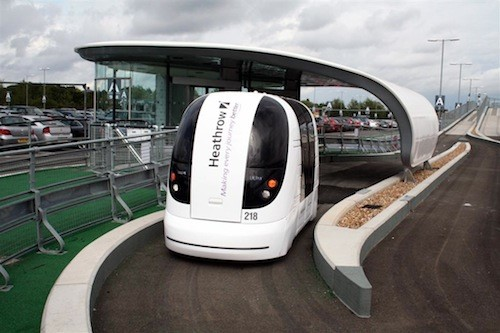
\includegraphics[width=0.4\linewidth]{image/PRT} \caption{London Heathrow Airport Shuttle (Kraft, 2012)}\label{fig:unnamed-chunk-46}
\end{figure}

The reasons for such a limited appearance are scare technical capabilities and scalability of PRT systems along with high capital and operating costs (Furman et al., 2014, p.~36).

\hypertarget{relevant-initiatives-in-austria-50}{%
\subsection*{Relevant initiatives in Austria}\label{relevant-initiatives-in-austria-50}}
\addcontentsline{toc}{subsection}{Relevant initiatives in Austria}

\begin{itemize}
\tightlist
\item
  \href{https://waset.org/personal-rapid-transit-and-system-design-conference-in-june-2023-in-vienna}{17th International Conference on Personal Rapid Transit and System Design in 2023}
\end{itemize}

\hypertarget{impacts-with-respect-to-sustainable-development-goals-sdgs-50}{%
\subsection*{Impacts with respect to Sustainable Development Goals (SDGs)}\label{impacts-with-respect-to-sustainable-development-goals-sdgs-50}}
\addcontentsline{toc}{subsection}{Impacts with respect to Sustainable Development Goals (SDGs)}

\begin{longtable}[]{@{}
  >{\centering\arraybackslash}p{(\columnwidth - 8\tabcolsep) * \real{0.2029}}
  >{\centering\arraybackslash}p{(\columnwidth - 8\tabcolsep) * \real{0.1884}}
  >{\centering\arraybackslash}p{(\columnwidth - 8\tabcolsep) * \real{0.2029}}
  >{\centering\arraybackslash}p{(\columnwidth - 8\tabcolsep) * \real{0.2029}}
  >{\centering\arraybackslash}p{(\columnwidth - 8\tabcolsep) * \real{0.2029}}@{}}
\toprule()
\begin{minipage}[b]{\linewidth}\centering
Impact level
\end{minipage} & \begin{minipage}[b]{\linewidth}\centering
Indicator
\end{minipage} & \begin{minipage}[b]{\linewidth}\centering
Impact direction
\end{minipage} & \begin{minipage}[b]{\linewidth}\centering
Goal description and number
\end{minipage} & \begin{minipage}[b]{\linewidth}\centering
Source
\end{minipage} \\
\midrule()
\endhead
Individual & Adverse impact on visual aspect of urban spaces & \textbf{-} & Health \& Wellbeing (\emph{3}) & Staniscia, 2018 \\
Systemic & Grade separation increases safety & \textbf{+} & Health \& Wellbeing (\emph{3}) & Juster \& Schonfeld, 2013; Furman et al., 2014 \\
Systemic & Electric power used & \textbf{+} & Environmental sustainability (\emph{7,12,13,15}) & Juster \& Schonfeld, 2013 \\
Systemic & Limited adoption worldwide & \textbf{-} & Innovation \& Infrastructure (\emph{9}) & Furman et al., 2014 \\
\bottomrule()
\end{longtable}

\hypertarget{technology-and-societal-readiness-level-50}{%
\subsection*{Technology and societal readiness level}\label{technology-and-societal-readiness-level-50}}
\addcontentsline{toc}{subsection}{Technology and societal readiness level}

\begin{longtable}[]{@{}cc@{}}
\toprule()
TRL & SRL \\
\midrule()
\endhead
5-8 & 5-7 \\
\bottomrule()
\end{longtable}

\hypertarget{open-questions-48}{%
\subsection*{Open questions}\label{open-questions-48}}
\addcontentsline{toc}{subsection}{Open questions}

\begin{enumerate}
\def\labelenumi{\arabic{enumi}.}
\tightlist
\item
  More research is needed on actual analysis of costs and benefits associated with the construction of PRT.
\item
  Can PRT infrastructure be considered and used as a attractive urban furniture? How can art community be engaged in its development?
\item
  What are the major barriers for more widespread adoption of PRT?
\end{enumerate}

\hypertarget{further-links-42}{%
\subsection*{Further links}\label{further-links-42}}
\addcontentsline{toc}{subsection}{Further links}

\begin{itemize}
\tightlist
\item
  \href{https://transweb.sjsu.edu/sites/default/files/1227-automated-transit-networks.pdf}{MIT Report}
\end{itemize}

\hypertarget{references-50}{%
\subsection*{References}\label{references-50}}
\addcontentsline{toc}{subsection}{References}

\begin{itemize}
\tightlist
\item
  Furman, B., Fabian, L., Ellis, S., Muller, P., \& Swenson, R. (2014). Automated transit networks (ATN): A review of the state of the industry and prospects for the future.
\item
  Juster, R., \& Schonfeld, P. (2013). Comparative analysis of personal rapid transit as an urban transportation mode. Transportation research record, 2350(1), 128-135.
\item
  Kraft, A. (2012). The beginning of personal rapid transit. Available at: \url{https://www.zdnet.com/article/the-beginning-of-personal-rapid-transit/} {[}Accessed: 21 Oct 2021{]}
\item
  Mobolaji, K., Földes, D., \& Csiszár, C. (2021). Concept of Advanced Personal Rapid Transit at Airports. Periodica Polytechnica Civil Engineering, 65(1), 320-334.
\item
  Staniscia, S. (2018). Aesthetic appreciation of Personal Rapid Transit: A new viewpoint. Cities, 79, 169-177.
\end{itemize}

\hypertarget{brt}{%
\section{Bus rapid transit}\label{brt}}

\hypertarget{synonyms-46}{%
\subsection*{Synonyms}\label{synonyms-46}}
\addcontentsline{toc}{subsection}{Synonyms}

\emph{High-level bus transport (HLBT)}

\hypertarget{definition-51}{%
\subsection*{Definition}\label{definition-51}}
\addcontentsline{toc}{subsection}{Definition}

Cities worldwide are looking for expanding the capacity of their public transport system while considering budget limitations (Ishaq \& Cats, 2020). Bus Rapid Transit (BRT) systems are increasingly being considered as alternatives for designing mass public transport in medium-sized cities in developed countries to reduce traffic congestion with its harmful effects on public health, the economy and the environment. Bus Rapid Transit (BRT) systems are high-quality bus-based transport systems that provide fast and efficient service (Abbasi et al., 2020). This is achieved by providing dedicated lanes, with busways and stations typically aligned with the centre of the street, off-board fare collection, and fast and frequent operations. Because BRT has similar features to a \protect\hyperlink{lrt}{light rail} or metro system, it is much more reliable, convenient and faster than a regular bus service. With the right features, BRT is able to avoid the causes of delays that typically slow down regular bus services, such as being caught in traffic and waiting in line to pay on board (ITDP, 2021b).

The term Bus Rapid Transit (BRT) originated in North America and is increasingly used elsewhere. The same concept is expressed by different names in different places (Deng \& Nelson, 2010):

\begin{itemize}
\tightlist
\item
  High-capacity bus systems
\item
  High value bus systems
\item
  Metro bus
\item
  Surface metro
\item
  Rapid bus systems
\item
  Busway systems
\item
  High-level bus transport
\end{itemize}

BRT systems offer a high-capacity alternative to rail-based systems, which require significantly higher investment and a longer implementation time (Deng \& Nelson, 2010; Fageda, 2021). In large cities in emerging economies, particularly in Latin America and South Asia, BRT is an integral part of, or forms the main part of, the mass public transport network. In contrast, BRT implementation in developed economies is mainly limited to medium-sized cities where demand levels do not justify large investments in urban rail infrastructure. In the European context, these projects are sometimes referred to as high service buses (BHLS) (Ishaq \& Cats, 2020).

\textbf{BRT basics}
There are five essential features that define BRT. These features primarily result in a faster journey for passengers and make local travel more reliable and convenient (ITDP, 2021b). They are:

\begin{itemize}
\tightlist
\item
  Dedicated right-of-way: Bus-only dedicated lanes provide a faster journey and ensure that buses are not delayed due to congestion in a mixed traffic.
\item
  Bus lane alignment: The centre of the lane or bus-only corridor keeps buses away from busy kerbs where cars park, stand and turn.
\item
  Fare collection: Paying the fare at the bus stop, rather than on the bus, eliminates the delay caused by passengers waiting on board.
\item
  Treatment of intersections: Prohibiting traffic from turning across the bus lane reduces bus delays caused by turning traffic. Prohibiting such turns is the most important measure to move buses through intersections - even more important than \protect\hyperlink{public_trans_priority}{signal priority}.
\item
  Platform level boarding: The bus stop should be level with the bus for quick and easy boarding. This makes it accessible to wheelchairs, disabled passengers, prams and walkers with minimal delays.
\end{itemize}

To be considered a BRT, a corridor must (ITDP, 2021b, 2021a):

\begin{itemize}
\tightlist
\item
  Be at least 3 km long;
\item
  Score 4 or more points in the dedicated right-of-way element;

  \begin{itemize}
  \tightlist
  \item
    8 points: Physically separated, dedicated lanes (e.g.~fences, curbs, bus stations)\\
  \item
    6 points: Colour-differentiated, dedicated lanes with no physical separation
  \item
    4 points: Dedicated lanes separated by a painted line
  \item
    0 points: No dedicated lanes
  \end{itemize}
\item
  Score 4 or more points in the bus alignment element;

  \begin{itemize}
  \tightlist
  \item
    8 points: Two-way bus lane with median in the middle strip of a two-way road
  \item
    8 points: Bus-only corridor in which there is a fully exclusive right-of-way and no parallel mixed traffic or converted corridor
  \item
    8 points: Busway that runs along a boundary condition such as a boardwalk or park where there are few intersections that cause conflicts
  \end{itemize}
\item
  Score 20 or more points in all five basic BRT elements

  \begin{itemize}
  \tightlist
  \item
    Dedicated right of way (up to 8 points)

    \begin{itemize}
    \tightlist
    \item
      Best practice: The Rainbow BRT Sangamwadi-Vishrantwadi corridor (Pune/Pimpri-Chinchwad, India), which uses fencing to create dedicated, physically separated bus lanes.
    \end{itemize}
  \item
    Busway alignment (up to 8 points)

    \begin{itemize}
    \tightlist
    \item
      Best practice: The Metrobus Green Line (Lahore, Pakistan), which includes a two-way median-aligned busway in the median of an roadway.
    \end{itemize}
  \item
    Off-board fare collection (up to 8 points)

    \begin{itemize}
    \tightlist
    \item
      Best practice: The TransJakarta Koridor 1 (Jakarta, Indonesia) offers off-board ticketing with turnstile-controlled access to stations
    \end{itemize}
  \item
    Intersection treatments (up to 7 points)

    \begin{itemize}
    \tightlist
    \item
      Best practice: Corredor Metropolitano ABD (São Paulo, Brazil) that prioritizes pedestrians and bans left-turns at intersections.
    \end{itemize}
  \item
    Boarding at platform level (up to 7 points)

    \begin{itemize}
    \tightlist
    \item
      Best practice: Ahmedabad BRTS (Ahmedabad, India) that, through well-designed infrastructure and driver training, has been able to reduce the boarding distance to less than 10 centimetres.
    \end{itemize}
  \end{itemize}
\end{itemize}

For more information on scoring system see \href{https://www.itdp.org/library/standards-and-guides/the-bus-rapid-transit-standard/the-scorecard/}{scorecard}.

\textbf{Open vs.~closed}
BRT combines stations, vehicles and technology into a high-quality, rail-like and can help improve urban mobility. The resurgence of bus-based transport in recent years has attracted great interest from transport and urban planners as it offers flexible, high-quality services at a lower cost than a rail-based transport system. With many successful systems around the world, investment in BRT has skyrocketed. One of the advantages of BRT is the flexibility of system design of corridors and stations. BRT can use buses operating in a variety of traffic conditions, such as mixed traffic, dedicated lanes on rural roads, and busways (highways or lanes of a highway reserved for the exclusive use of BRT). In North America, most BRT systems use separate or segregated lanes, while in South America BRT systems use the centre lanes. Another advantage of BRT is the operational flexibility to integrate with existing conventional bus services.

BRT can operate as either an open or closed system. A closed system means that BRT buses can only operate on the BRT corridor and non-BRT buses cannot operate on the BRT corridor (Zhang et al., 2020b). Users typically view a closed BRT system as a frequent and on-time rail-like service that eliminates most of the typical causes of delay that occur with conventional bus services (Zhang et al., 2020a). Some newer BRT systems (Seoul in South Korea, Guangzhou in China and Sydney, Adelaide and Brisbane in Australia) have adopted an open system approach where conventional buses enter and exit the BRT corridor. These open BRT services allow passengers to reach the BRT corridor without changing buses. In an open BRT system, they can effectively improve BRT accessibility for passengers away from the BRT corridor by eliminating the disadvantages associated with transferring, as well as additional walking and waiting time (Yen et al., 2018). However, local traffic may affect these feeder services that use the BRT corridor for part of their routes, reducing the overall performance of the BRT service. On the other hand, since bus-based systems are flexible, sometimes a hybrid mode of operation could also be suitable. Transport planners can review bus routes to identify high ridership routes and operate an open BRT for these routes and add additional services operating as a closed system for other low ridership routes and design a network of feeder buses for these services. This concept can be applied to different times of the day, with the BRT corridor being an open system during off-peak hours to allow for single occupancy trips and closed during peak hours to relieve overcrowding and congestion (Zhang et al., 2020b).

\hypertarget{key-stakeholders-51}{%
\subsection*{Key stakeholders}\label{key-stakeholders-51}}
\addcontentsline{toc}{subsection}{Key stakeholders}

\begin{itemize}
\tightlist
\item
  \textbf{Affected}: Mobile citizen, Public transport users
\item
  \textbf{Responsible}: National governments, City government, Private Companies, Transport agencies, Infrastructure providers, Bus manufacturers
\end{itemize}

\hypertarget{current-state-of-art-in-research-51}{%
\subsection*{Current state of art in research}\label{current-state-of-art-in-research-51}}
\addcontentsline{toc}{subsection}{Current state of art in research}

Many researchers focus on local BRT systems with different emphases such as Malik et al.~(2021) investigates user travel behaviour in Lahore, Kiani. Mavi et al.~(2018) evaluates and optimises a BRT line in Tehran (Iran) using a simulation and multi-criteria decision-making approach. Ishaq \& Cats (2020) report empirical findings from the implementation of a BRT system in Haifa (Israel). Finally, Mallqui \& Pojani (2017) compares Bus Rapid Transit (BRT) issues in Brisbane (Australia) with Lima (Peru). Citizen participation has taken place in both cities. Regardless of competition from other modes of transport, both BRT systems have been positively received by the local population. In particular, people who live close to the stations and can use the BRTs for their commute to work are very positive about this mode of transport.
Schwanen \& Ferbrache (2017) from the Transport Studies Unit at the University of Oxford have compiled a list of literature on the wider economic and social impacts of Bus Rapid Transit (BRT). The following topics are covered by the literature:

\begin{itemize}
\tightlist
\item
  BRT impact studies, which examine wider economic and social impacts of BRT.
\item
  Land development, land use change and/or transport-oriented development.
\item
  change in land/property values
\item
  new economic development
\item
  accessibility of jobs/workplaces
\item
  improvement of the urban environment
\item
  prestige/reputation of the city
\item
  physical displacement of poorer households
\end{itemize}

Several researchers have investigated the effect of Bus Rapid Transit (BRT) on property values (Zhang et al., 2020a; Zhang \& Yen, 2020)). Zhang \& Yen (2020) compared 23 other studies on this topic and the two main conclusions are:

\begin{itemize}
\tightlist
\item
  The estimated increase in value for land is much higher than for real estate (i.e.~27.5\% higher).
\item
  In general, land and real estate within 50 m of a BRT station have a price premium of 13.0\% compared to land and real estate 1,2 km away.
\end{itemize}

These results can help to better understand the accessibility benefits of BRT systems, especially where empirical evidence is lacking. However, evidence from European BRT systems is lacking and few studies have examined how BRT systems affect land and property values over time.

Basso et al.~(2019) proposed a dynamic congestion approach that endogenously models queues both on the road and at BRT stations. Some of the key findings are:

\begin{itemize}
\tightlist
\item
  The optimal BRT is efficient in terms of total cost, and even with imperfectly divisible capacity, BRT is still the better choice for many demand levels (starting with demands between 8000 and 8500 commuters).
\item
  Without BRT, there is a large demand cut interval where it is optimal to offer no public transport (up to 10,000 commuters). However, if part of the road capacity were dedicated exclusively to buses, then optimally buses would have to run very frequently. Urban planners should, therefore, plan BRT systems from the outset, rather than gradually integrating public transport until demand becomes so high that traffic congestion occurs. Thus, bus frequencies will become more frequent and dedicated bus lanes will become ``necessary''.
\item
  The operating times of buses and cars are much shorter with BRT than under mixed traffic conditions. Therefore, although BRT takes capacity away from car traffic, it will reduce the peak time of car traffic.
\end{itemize}

Abbasi et al.~(2020) studied different aspects of BRT in Tehran (Iran). In their simulations, exclusive bus lanes had good effects on reducing pollutant emissions and fuel consumption. On average, the exclusive bus lanes scenarios would reduce CO emissions from buses by 40.6\% and increase CO emissions from cars by 3.1\%, NOx (buses reduced by 15.1\%; cars increased by 6.7\%), PM (buses reduced by 6.7\%; cars increased by 4.4\%) and fuel consumption (buses reduced by 5.6\%; cars increased by 3.2\%). In the scenarios of efficient use and standardisation of the number of stations, not only the pollutant emissions of the buses are reduced, but also those of the passenger cars. One possible reason for this is the reduction of conflicts between buses and cars on shared lanes. In the scenario of implementing switched traffic lights and bus priority, pollutant emissions and fuel consumption of buses decrease by 10.2\% on average, while they increase by 1.3\% for passenger cars. From an economic point of view, the full exclusive bus lane had the highest reduction in annual costs.

\hypertarget{current-state-of-art-in-practice-51}{%
\subsection*{Current state of art in practice}\label{current-state-of-art-in-practice-51}}
\addcontentsline{toc}{subsection}{Current state of art in practice}

BRT systems initially thrived in Latin American cities (Dario Hidalgo \& Graftieaux, 2008), before spreading to South and East Asia and then across the world (Darío Hidalgo \& Gutiérrez, 2013). However, although the number of BRT systems is increasing worldwide, only \textasciitilde10\% of BRT systems are currently located in low- and middle-income countries (Malik et al., 2021).

According to (Global BRTData, 2021), the distribution of BRT systems worldwide (as of 2021) in terms of number of passengers (worldwide daily 33,684,575) is divided into Africa with 491,578 passengers (1.45\%), Asia 9,238,060 (27.42\%), Europe 1,613,580 (4.79\%), Latin America 20,916,474 (62.09\%), Northern America 988,683 (2.93\%) and Oceania 436,200 (1.29\%).

Three new BRT systems established in Australia (Busway in Adelaide, Brisbane and Sydney) are open systems. This could be due to the characteristics of Australian urban areas, which tend to have low population density and high car use. Since passengers have to transfer, it is more difficult for a closed system to take advantage of the network effect, and an open BRT system might be more attractive in this car-dominated environment. However, Brisbane is considering switching to a closed BRT operating system due to serious congestion issues, particularly during peak hours (Zhang et al., 2020b).

Daimler says that more and more Europeans are recognising the advantages of effective and attractive urban bus transport systems. France is cited as a pioneer, where the government is supporting the expansion of BRT systems with large sums of money (Daimler (EvoBus GmbH), n.d.). This is implemented by the world's first hydrogen-powered express bus system that has gone into operation under the name Fébus in the French city of Pau. Eight ExquiCity18 Fuel Cell van-hool buses in tram design are used. The 18-metre-long articulated buses offer space for 125 passengers and can cover more than 300 kilometres per hydrogen filling (Schaal, 2019).

Further, two BRT lines will be introduced for the public transport system in Florence. The two lines will complete the network of public transport on the road to relieve the buses that currently operate on these routes. This innovation is made possible by the Metrocittà Sustainable Mobility Plan (autobusweb.com, 2021).

In Istanbul, the BRT network already stretches over a total of 52 kilometres and transports 750,000 passengers daily. Cities like Amsterdam, Strasbourg and Paris already operate their own BRT system. In Germany, BRT has not yet been implemented, as rail is still the first resort. According to Richard Mejía (head of the BRT team at Daimler Buses), the investment and operating costs are lower compared to rail systems. About the future development of BRT, it is mentioned that the previous concept is constantly being developed and adapted to new technologies or current urban planning. The course is currently being set for emission-free driving with electric mobility. Also, partially autonomous driving of buses (for example, the Future Bus from Mercedes-Benz, which was presented in mid-2016) could reduce fuel consumption through constant acceleration and braking behaviour. Extended and intelligent networking, for example between vehicles, signalling systems and the roadway, will also make BRT systems even more attractive in the future (Daimler AG, n.d.).

\hypertarget{relevant-initiatives-in-austria-51}{%
\subsection*{Relevant initiatives in Austria}\label{relevant-initiatives-in-austria-51}}
\addcontentsline{toc}{subsection}{Relevant initiatives in Austria}

Carinthia could get a rapid bus system for local transport.

\begin{itemize}
\tightlist
\item
  \href{https://kaernten.orf.at/stories/3029225/}{Kaernten.orf.at}
\end{itemize}

Currently, eleven rapid bus transit lines, so-called \emph{Schnellbussystem} (without dedicated lines), connect the centres of the 3 surrounding districts with the provincial capital of St.~Pölten. The fleet consists of 47 vehicles in four different sizes in the uniform Wiesel design, which together offer a seating capacity for 2,449 passengers.

\begin{itemize}
\tightlist
\item
  \href{https://www.meinbezirk.at/st-poelten/c-lokales/wieselbus-erfolgsstory-feiert-20-jahre_a1863287}{Meinbezirk.at}
\end{itemize}

\hypertarget{impacts-with-respect-to-sustainable-development-goals-sdgs-51}{%
\subsection*{Impacts with respect to Sustainable Development Goals (SDGs)}\label{impacts-with-respect-to-sustainable-development-goals-sdgs-51}}
\addcontentsline{toc}{subsection}{Impacts with respect to Sustainable Development Goals (SDGs)}

\begin{longtable}[]{@{}
  >{\centering\arraybackslash}p{(\columnwidth - 8\tabcolsep) * \real{0.2029}}
  >{\centering\arraybackslash}p{(\columnwidth - 8\tabcolsep) * \real{0.1884}}
  >{\centering\arraybackslash}p{(\columnwidth - 8\tabcolsep) * \real{0.2029}}
  >{\centering\arraybackslash}p{(\columnwidth - 8\tabcolsep) * \real{0.2029}}
  >{\centering\arraybackslash}p{(\columnwidth - 8\tabcolsep) * \real{0.2029}}@{}}
\toprule()
\begin{minipage}[b]{\linewidth}\centering
Impact level
\end{minipage} & \begin{minipage}[b]{\linewidth}\centering
Indicator
\end{minipage} & \begin{minipage}[b]{\linewidth}\centering
Impact direction
\end{minipage} & \begin{minipage}[b]{\linewidth}\centering
Goal description and number
\end{minipage} & \begin{minipage}[b]{\linewidth}\centering
Source
\end{minipage} \\
\midrule()
\endhead
Systemic & Reduction in pollutant emissions and fuel consumption & \textbf{+} & Environmental sustainability (\emph{7,12,13,15}) & Abbasi et al., 2020 \\
Systemic & BRT requires significantly shorter investments and implementation time & \textbf{+} & Innovation \& Infrastructure (\emph{9}) & Deng \& Nelson, 2010; Fageda, 2021 \\
\bottomrule()
\end{longtable}

\hypertarget{technology-and-societal-readiness-level-51}{%
\subsection*{Technology and societal readiness level}\label{technology-and-societal-readiness-level-51}}
\addcontentsline{toc}{subsection}{Technology and societal readiness level}

\begin{longtable}[]{@{}cc@{}}
\toprule()
TRL & SRL \\
\midrule()
\endhead
7-9 & 7-9 \\
\bottomrule()
\end{longtable}

\hypertarget{open-questions-49}{%
\subsection*{Open questions}\label{open-questions-49}}
\addcontentsline{toc}{subsection}{Open questions}

\begin{enumerate}
\def\labelenumi{\arabic{enumi}.}
\tightlist
\item
  How can development of BRT systems be supported in a better way through national policies?
\end{enumerate}

\hypertarget{further-links-43}{%
\subsection{Further links}\label{further-links-43}}

\begin{itemize}
\tightlist
\item
  \href{http://brtdata.org/}{BRT data}
\item
  \href{https://www.itdp.org/library/standards-and-guides/the-bus-rapid-transit-standard/what-is-brt/}{What is BRT?}
\item
  \href{https://www.itdp.org/library/standards-and-guides/the-bus-rapid-transit-standard/the-scorecard/}{Scorecard}
\item
  \href{https://www.transit.dot.gov/sites/fta.dot.gov/files/issues.pdf}{BRT issues}
\end{itemize}

\hypertarget{references-51}{%
\subsection*{References}\label{references-51}}
\addcontentsline{toc}{subsection}{References}

\begin{itemize}
\tightlist
\item
  Abbasi, M. H., Hadji Hosseinlou, M., \& JafarzadehFadaki, S. M. (2020). An investigation of Bus Rapid Transit System (BRT) based on economic and air pollution analysis (Tehran, Iran). Case Studies on Transport Policy, 8(2), 553--563. \url{https://doi.org/10.1016/j.cstp.2019.11.008}
\item
  autobusweb.com. (2021, March 2). Trasporto pubblico Firenze, in arrivo due linee Bus Rapid Transit. \url{https://www.autobusweb.com/tpl-firenze-in-arrivo-due-linee-bus-rapid-transit/}
\item
  Basso, L. J., Feres, F., \& Silva, H. E. (2019). The efficiency of bus rapid transit (BRT) systems: A dynamic congestion approach. Transportation Research Part B: Methodological, 127, 47--71. \url{https://doi.org/10.1016/j.trb.2019.06.012}
\item
  Daimler (EvoBus GmbH). (n.d.). Bus Rapid Transit (BRT) in Europe -- Impressions of a sustainable mobility concept in Strasbourg - EvoBus GmbH. Available at: \url{https://www.evobus.com/de-en/layer/bus-rapid-transit-brt-in-europe-impressions-of-a-sustainable-mobility-concept-in-strasbourg/} {[}Accessed: 24 June 2021{]}
\item
  Daimler AG. (n.d.). Bus Rapid Transit -- Neue Unabhängigkeit im Stadtverkehr \textbar{} Daimler. Available at: \url{https://www.daimler.com/nachhaltigkeit/staedte/bus-rapid-transit.html} {[}Accessed: 24 June 2021{]}
\item
  Deng, T., \& Nelson, J. D. (2010). Transport Reviews Recent Developments in Bus Rapid Transit: A Review of the Literature. \url{https://doi.org/10.1080/01441647.2010.492455}
\item
  Fageda, X. (2021). Do light rail systems reduce traffic externalities? Empirical evidence from mid-size european cities. Transportation Research Part D: Transport and Environment, 92, 102731. \url{https://doi.org/10.1016/j.trd.2021.102731}
\item
  Global BRTData. (2021). Global BRTData. Brtdata.Org. \url{http://brtdata.org/}
\item
  Hidalgo, Dario, \& Graftieaux, P. (2008). Bus Rapid Transit Systems in Latin America and Asia: Results and Difficulties in 11 Cities. Transportation Research Record, 2072(1), 77--88. \url{https://doi.org/10.3141/2072-09}
\item
  Hidalgo, Darío, \& Gutiérrez, L. (2013). BRT and BHLS around the world: Explosive growth, large positive impacts and many issues outstanding. Research in Transportation Economics, 39(1), 8--13. \url{https://doi.org/10.1016/j.retrec.2012.05.018}
\item
  Ishaq, R., \& Cats, O. (2020). Designing bus rapid transit systems: Lessons on service reliability and operations. Case Studies on Transport Policy, 8(3), 946--953. \url{https://doi.org/10.1016/j.cstp.2020.05.001}
\item
  ITDP. (2021a). The Scorecard - Institute for Transportation and Development Policy. \url{https://www.itdp.org/library/standards-and-guides/the-bus-rapid-transit-standard/the-scorecard/}
\item
  ITDP. (2021b). What is BRT? - Institute for Transportation and Development Policy. \url{https://www.itdp.org/library/standards-and-guides/the-bus-rapid-transit-standard/what-is-brt/}
\item
  Kiani Mavi, R., Zarbakhshnia, N., \& Khazraei, A. (2018). Bus rapid transit (BRT): A simulation and multi criteria decision making (MCDM) approach. Transport Policy, 72, 187--197. \url{https://doi.org/10.1016/j.tranpol.2018.03.010}
\item
  Malik, B. Z., Rehman, Z. ur, Khan, A. H., \& Akram, W. (2021). Investigating users' travel behaviours and perceptions of single-corridor BRT: Lessons from Lahore. Journal of Transport Geography, 91, 102942. \url{https://doi.org/10.1016/j.jtrangeo.2020.102942}
\item
  Mallqui, Y. Y. C., \& Pojani, D. (2017). Barriers to successful Bus Rapid Transit expansion: Developed cities versus developing megacities. Case Studies on Transport Policy, 5(2), 254--266. \url{https://doi.org/10.1016/j.cstp.2017.01.004}
\item
  Schaal, S. (2019, December 18). Fébus: Erstes H2-Schnellbussystem in Betrieb - electrive.net. \url{https://www.electrive.net/2019/12/18/febus-erstes-h2-schnellbussystem-in-betrieb/}
\item
  Schwanen, T., \& Ferbrache, F. (2017). Bibliography of Research on Bus Rapid Transit. 1068. \url{https://www.tsu.ox.ac.uk/pubs/1068-schwanen-ferbrache.pdf}
\item
  Yen, B. T. H., Mulley, C., Tseng, W. C., \& Chiou, Y. C. (2018). Assessing interchange effects in public transport: A case study of South East Queensland, Australia. Case Studies on Transport Policy, 6(3), 364--375. \url{https://doi.org/10.1016/j.cstp.2018.01.005}
\item
  Zhang, M., \& Yen, B. T. H. (2020). The impact of Bus Rapid Transit (BRT) on land and property values: A meta-analysis. Land Use Policy, 96, 104684. \url{https://doi.org/10.1016/j.landusepol.2020.104684}
\item
  Zhang, M., Yen, B. T. H., Mulley, C., \& Sipe, N. (2020a). An investigation of the open-system Bus Rapid Transit (BRT) network and property values: The case of Brisbane, Australia. Transportation Research Part A: Policy and Practice, 134, 16--34. \url{https://doi.org/10.1016/j.tra.2020.01.021}
\item
  Zhang, M., Yen, B. T. H., Mulley, C., \& Sipe, N. (2020b). How does an open system bus rapid transit (BRT) facilitate inter and intra-modal mobility? A visual analytic analysis of Brisbane, Australia. Research in Transportation Economics, 83, 100906. \url{https://doi.org/10.1016/j.retrec.2020.100906}
\end{itemize}

\hypertarget{lrt}{%
\section{Light rail transit}\label{lrt}}

\hypertarget{synonyms-47}{%
\subsection*{Synonyms}\label{synonyms-47}}
\addcontentsline{toc}{subsection}{Synonyms}

\emph{Light Rail Transit (LRT), Heavy Rail Transit (HRT)}

\hypertarget{definition-52}{%
\subsection*{Definition}\label{definition-52}}
\addcontentsline{toc}{subsection}{Definition}

Light rail (also referred to as tram) has become a popular measure among urban planners to address the social and economic complexities associated with urban growth (Baker \& Lee, 2019). Light rail developments go beyond improving access to public transport to surrounding neighbourhoods. Impacts can also address property values, neighbourhood demographics, employment opportunities and access to services (Hess, 2020).

Proponents argue that the establishment of new LRT lines can promote environmental sustainability by reducing private car use and improve public health by increasing neighbourhood walkability and air quality (D. Knowles \& Ferbrache, 2016). Other arguments are that LRTs address income inequality positively by encouraging business development and providing direct access to employment centres in a city or suburb (Hess, 2020).

Many of these impacts have implications for the health and well-being of residents. These are assessed through the social determinants of health (SDOH). The World Health Organization (WHO) defines the social determinants of health (SDOH) as the ``\emph{conditions under which people are born, grow up, live, work and age}'' (e.g.~income, housing, employment) and ``\emph{the underlying drivers of these conditions}'' (e.g.~economic and social policies and political systems) (Braveman \& Gottlieb, 2014). The SDOH framework asserts that the way political, social and economic resources are distributed within communities can have an impact on health and well-being (Solar \& Irwin, 2010).

LRT has become a popular form of transit due to low construction costs compared to underground systems and large perceived economic benefits. LRT systems are typically built along existing streets, eliminating the need for expensive tunnel or elevated rail infrastructure. While LRT shares road space with vehicles and pedestrians, portions of the routes are used with priority, allowing for higher speeds and fewer delays than buses. Unlike bus transit, the need for rails, an above-ground power source and platforms ensures that LRT is a long-term local investment (Tyndall, 2021).

Laird (2019) defines the differences between light rail systems and commuter rail systems. They function differently, have different requirements and use different systems for operation:

\textbf{Commuter rail systems}
Commuter rail systems are passenger trains that run on diesel-electric or electrically powered engines. They operate on existing railway tracks on the same routes used by intercity goods trains. They are operated by state authorities or private companies on their own or third-party tracks. They typically have speeds of 80 to 130 km/h, shorter routes and are usually only found in larger conurbations. Commuter rail systems have fewer stops than light rail and typically run through suburbs and central cities. Because commuter rail systems are designed for commuters, the schedule frequency may be different than light rail and run less frequently throughout the day. Commuter rail systems often run most frequently during standard commuting hours for the average workday.

\textbf{Light rail systems}
Light rail systems are passenger trains powered by overhead electric wires. They have lighter frames and smaller bodies than other trains due to the turning radius required. Because light rail systems operate in city streets and urban corridors with frequent stops, they have a smaller turning radius to weave in and out of busy areas and can accelerate and decelerate faster than commuter rail. While commuter rail systems can run over existing goods train tracks, light rail systems generally require their own tracks.

\hypertarget{key-stakeholders-52}{%
\subsection*{Key stakeholders}\label{key-stakeholders-52}}
\addcontentsline{toc}{subsection}{Key stakeholders}

\begin{itemize}
\tightlist
\item
  \textbf{Affected}: Pedestrians, Public transport users, Local residents, Drivers
\item
  \textbf{Responsible}: City governments, Private Transport Companies, Transport Authorities
\end{itemize}

\hypertarget{current-state-of-art-in-research-52}{%
\subsection*{Current state of art in research}\label{current-state-of-art-in-research-52}}
\addcontentsline{toc}{subsection}{Current state of art in research}

Research mainly examines the social impacts (Baker \& Kim, 2020; Baker \& Lee, 2019; Deyas \& Woldeamanuel, 2020; Hess, 2020; Tyndall, 2021) and the economic impacts (D. Knowles \& Ferbrache, 2016) of light rail transit.

Knowles \& Ferbrache (2016) assess the wider economic impacts of light rail investment on cities. They focused on evidence from UK, European and North American case studies, as there is still a lack of light rail research from less developed cities around the world. They found that investments in light rail systems can have positive economic impacts on cities. However, similar light rail investments in different locations do not necessarily have the same impact, therefore the geography matters. Similar to other forms of transport infrastructure, light rail investments alone are unlikely to be a sufficient catalyst for economic change without additional supporting measures.

Light rail can spur economic growth by improving accessibility to previously inaccessible areas, encouraging foreign investment, triggering new growth, expanding labour market catchment areas and influencing property prices. However, while many areas experience price increases following the construction of light rail, these are often not absorbed and the capital to fund the infrastructure has to be raised elsewhere. Therefore, as with other forms of public transport, the economic impact of light rail is enhanced when land use and transport planning policies are coordinated, and this is highly dependent on other contextual factors.

Tyndall (2021) notes that LRT effectively increases overall public transport use because it attracts higher-skilled workers who would be unlikely to use other forms of public transport, while low-skilled workers continue to use public transport.

\textbf{Automation of LRT}

\begin{itemize}
\tightlist
\item
  Level 2 automation refers to a system where trains run automatically from station to station, but there is a driver in the cab who is responsible for closing the doors, detecting obstacles on the track in front of the train and handling emergency situations.
\item
  In automation level 3, trains run automatically from station to station, but there is always a staff member on the train who is responsible for handling emergency situations.
\item
  In automation level 4, trains are able to run automatically at all times, including door closure, obstacle detection and emergency situations. On-board staff may be provided for other purposes, such as customer service, but are not required for safe operation. Controls are often provided to manually operate the train in the event of a computer failure. Examples so far are only Metros in Paris, Barcelona, Sydney and Copenhagen (UITP, n.d.). Trams have only been tested for autonomous driving since 2018.
\end{itemize}

\hypertarget{current-state-of-art-in-practice-52}{%
\subsection*{Current state of art in practice}\label{current-state-of-art-in-practice-52}}
\addcontentsline{toc}{subsection}{Current state of art in practice}

Trams and light rail systems exist in 389 cities worldwide, more than half (204) of them in Europe. Between 2015 and 2018, the light rail infrastructure in Europe grew by 3.9\% from 8943 km to 9296 km, and passenger numbers increased by 6.9\% from 9740 million to 10,422 million passengers. Light rail transit systems now carry as many passengers as metros and regional/suburban rail lines and ten times more passengers than air travel in Europe.
The average light rail journey in Europe is 3.27 km. The busiest light rail network in Europe is in Budapest, Hungary, with 411 million passengers, while Berlin has the longest light rail network in Europe with 193 km. Passenger growth varies from region to region, ranging from 17.5\% in the British Isles to 1.5\% in Poland.

While the average European line is 7.3 km long, they tend to be longer on average in countries with newer systems and a limited number of lines, while older, more complex systems have a lower average line length. Europe's fleet consists of 20,750 trams and light rail vehicles, with 51\% of this fleet consisting of partial or full low-floor vehicles, ranging from countries with almost 100\% such as France, Spain, Ireland, the UK and Norway to countries with much lower proportions. The average annual mileage per vehicle in Europe is 52,000 km, ranging from 38,700 km to 77,500 km (this value is theoretical and based on the assumption that all vehicles are used equally). According to UITP, light rail will continue to receive support from decision-makers and the travelling public in Europe, given the ongoing pressure to reduce congestion, tackle poor air quality in cities and reduce greenhouse gas emissions contributing to climate change. However, much attention and resources will go into maintaining, upgrading and replacing facilities to keep ageing systems attractive and operational. For this reason, the growth of greenfield projects in Europe will continue to slow down (Burroughs, 2020; UITP, 2019).

\textbf{Examples of recent investments}

\begin{itemize}
\item
  The Jerusalem tram project which involves building 27 km of new tram lines, 53 stations and a number of depots (Railway-News, 2019).
\item
  Lisbon public transport company, and CAF signed a contract for a new LRT line. The low-floor tram will have a length of 28.5 metres and will be able to run at a speed of 70 km/h (Railwaypro, 2021b).
\item
  Paris opens the new T9 LRT line between Paris and the city of Orly. The 40 km line has 19 stations and is expected to carry 70,000 to 80,000 passengers per day. The light rail vehicles have eight double doors per side and wider gangways to improve passenger flow and reduce boarding times (Burroughs, 2021).
  European cities will continue to invest in cleaner transport and logistics, including a boost for rail travel and clean mobility in cities and regions (European Commission, 2020). Also the World Bank, 2020 states that investing in reliable mass transit systems such as metro, LRT and Bus Rapid Transit can help keep cities moving while reducing the carbon footprint of urban transport.
\item
  US cities also have made significant investments in Light Rail Transit (LRT) in recent years. A common justification for LRT is that transit infrastructure improves urban commuter networks by creating spatial connections between workers and jobs. Between 2000 and 2015, the number of LRT stations in four metropolitan regions in the US grew by 56\% (Tyndall, 2021).
\item
  Moscow announced that the tram network will be managed by the Moscow Metro. It is expected that the centralised management and consistent modernisation will increase tram speeds, improve track maintenance, halve the number of repairs and reduce maintenance costs. In 2019, the tram network carried 212 million passengers, which is 12 times more than the population of Moscow. By 2023, Moscow plans to replace its entire existing old tram fleet with low-floor trams. It is expected that by 2024 only low-floor trams will operate on all Moscow routes (Railwaypro, 2021a).
\end{itemize}

Furthermore, the investments are also being made in tram-trains. A combination of Light rail and train. While as a train it has the travel advantages of a railway in the surrounding areas, such as speeds, safety standards, ride comfort, sanitary facilities and in the city centre it functions as a tram. These multi-system vehicles, with their equipment and operating characteristics, are ideally suited to the needs of passengers who travel longer distances by train, as well as for passengers who make only a few stops in the city centre. Above all, the tram-train vehicles also enable direct connections from surrounding areas to the city without changing trains. From the region to the city limits, passengers, thus, have the advantage of fast travel times and high passenger comfort (Seyringer, 2020). In Karlsruhe there are some examples of tram trains existing since 1992 (Stadtwiki Karlsruhe, 2016). They already have continuous rail connections between the inner cities and the regions (Stadtwiki Karlsruhe, 2020). Further, the Badner Bahn is also a well-known tram-train example. The 30.4 km long Badner Bahn tram system runs between Vienna and Baden. Every year, Wiener Lokalbahnen transports around 12 million passengers between Vienna and Baden. Commuters from the south of Vienna are particularly prone to use the Badner Bahn every day (RailwayPro, 2020).

\textbf{Automation}

For several decades now, the tram has been experiencing a renaissance worldwide. Cars and buses are becoming increasingly intelligent and independent thanks to advanced sensor and automation technology. If the tram wants to keep up and secure its attractiveness and competitiveness in the long term, it must evolve into a smart and autonomous means of transport. The automation technology works by using lidar, radar and cameras (Siemens Mobility, 2019):

\emph{Lidar (Light detection and ranging)}

\begin{itemize}
\tightlist
\item
  Enables 3D environmental detection and positioning
\item
  Scans objects vertically and horizontally with laser beams and horizontally; uses the reflected waves to perceive the surroundings
\item
  Enables the tram to ``see'' at an angle of up to 270°
\end{itemize}

\emph{Radar (Radio Detection and Ranging)}

\begin{itemize}
\tightlist
\item
  Measures distance and speed with high accuracy - especially of metallic objects
\item
  Emits radio waves and uses the reflected waves to locate objects
\item
  Covers a large area in front of the tram
\end{itemize}

\emph{Cameras}

\begin{itemize}
\tightlist
\item
  Are trained in intelligent object and signal recognition
\item
  Can detect and classify objects in thousands of contours and positions - e.g.~as people, signals or infrastructure elements
\item
  Cover a large optical area around the vehicle
\end{itemize}

A few years before 2020, Siemens Mobility launched the driver assistance system ``\emph{Siemens Tram Assistant}'' - a collision warning and protection system to support the driver. The system is already being used successfully in Siemens trams in Den Haag (Netherlands) and Ulm (Germany). The next commercially viable step planned is depot automation based on an autonomous tram. This will make it possible to automate time-consuming shunting operations in the depot, such as service runs through a car wash to a siding. The extensive isolation from public traffic simplifies technical control and approval (Hofmann, 2020; Zasiadko, 2019b).

The three leading countries in the development of autonomous trams are Germany, Russia and China (Intelligent Transport, 2019). Siemens Mobility is testing the first autonomous tram in an automated depot in Germany since 2018 (Hofmann, 2020). PC Transport Systems and Cognitive Technologies have announced a joint project that will develop a fully autonomous tram for the Russian and foreign markets by 2022 (Intelligent Transport, 2019; Zasiadko, 2019a). Following the successful tests of the autonomous tram in Moscow, the Russian company Cognitive Technologies is planning to develop an AI-based computer vision system for the Chinese market together with Fuxin Intelligent Transportation Solutions (FITSCO), one of the largest suppliers of signalling and communication solutions in China. This is needed for the testing and introduction of the self-driving trams in Shanghai. The project is to be implemented in 2021 (Zasiadko, 2020).

Unlike similar solutions for self-driving cars, the system for rail has a number of simplifications that will allow trams to run on public roads sooner. But despite these simplifications, there are only a few countries in the world that are ready for the real deployment of autonomous trams. The developed autonomous driving system recognises vehicles and other trams, traffic lights, pedestrians, tram and bus stops, railway switches and various obstacles. The tram is also able to stop in front of the obstacles, maintain a safe distance from the vehicles ahead, accelerate and stop (Intelligent Transport, 2019).

\hypertarget{relevant-initiatives-in-austria-52}{%
\subsection*{Relevant initiatives in Austria}\label{relevant-initiatives-in-austria-52}}
\addcontentsline{toc}{subsection}{Relevant initiatives in Austria}

Vienna has a number of expansion plans for the tram network planned for the coming decade, including connecting the Lower Austrian surrounding area with three lines. Such routes are now becoming more realistic. This is because both provinces are examining the possibilities and framework conditions for implementation in spring 2020 (Wiener Linien, 2020).

\begin{itemize}
\tightlist
\item
  \href{https://wien.orf.at/stories/3068577/}{Tram network extension plans}
\end{itemize}

``\emph{In addition to the 1-2-3-Klimaticket itself, Upper Austrians will also get an improved, innovative public transport infrastructure with the Linz-Gallneukirchen-Pregarten regional light rail system in the coming years and thus further incentives for commuters to travel to Linz by `tram-train' instead of standing in traffic jams on the S10 and A7}'' explains Weratschnig (Transport spokesman of the Green Party) (Grüner Klub im Parlament, 2021). Further, Badner Bahn will receive new trams. These will gradually replace the old high-floor models starting in the second half of 2021 (RailwayPro, 2020).

\begin{itemize}
\tightlist
\item
  \href{https://www.railwaypro.com/wp/interior-design-for-wiener-lokalbahnen-new-tram-unveiled/}{Badner Bahn}
\end{itemize}

Tram-Trains for Linz (Upper Austria) are expected in July 2026. The vehicles will have regional train seats, seating groups and luggage storage facilities in the middle section, while multi-purpose compartments for wheelchair, pram and bicycle transport are planned for the front and rear sections. The vehicles intended for use on the longer light rail routes will be equipped with toilets (Seyringer, 2020). In Salzburg, too, at least 20 new tram-trains are planned for Salzburg until 2026 (SALZBURG24, 2020).

\begin{itemize}
\tightlist
\item
  \href{https://www.salzburg24.at/news/salzburg/salzburger-lokalbahn-bekommt-neue-tram-trains-91192069}{Salzburg tram}
\item
  \href{https://www.ots.at/presseaussendung/OTS_20210312_OTS0128/grueneweratschnig-vom-muehlkreis-aus-bald-per-tram-train-nach-linz-statt-im-stau-auf-der-a7}{Linz tramtrain}
\item
  \href{https://kommunal.at/eisenbahn-und-stadtbahn-einem}{Tramtrain in Austria}
\end{itemize}

\hypertarget{impacts-with-respect-to-sustainable-development-goals-sdgs-52}{%
\subsection*{Impacts with respect to Sustainable Development Goals (SDGs)}\label{impacts-with-respect-to-sustainable-development-goals-sdgs-52}}
\addcontentsline{toc}{subsection}{Impacts with respect to Sustainable Development Goals (SDGs)}

\begin{longtable}[]{@{}
  >{\centering\arraybackslash}p{(\columnwidth - 8\tabcolsep) * \real{0.2029}}
  >{\centering\arraybackslash}p{(\columnwidth - 8\tabcolsep) * \real{0.1884}}
  >{\centering\arraybackslash}p{(\columnwidth - 8\tabcolsep) * \real{0.2029}}
  >{\centering\arraybackslash}p{(\columnwidth - 8\tabcolsep) * \real{0.2029}}
  >{\centering\arraybackslash}p{(\columnwidth - 8\tabcolsep) * \real{0.2029}}@{}}
\toprule()
\begin{minipage}[b]{\linewidth}\centering
Impact level
\end{minipage} & \begin{minipage}[b]{\linewidth}\centering
Indicator
\end{minipage} & \begin{minipage}[b]{\linewidth}\centering
Impact direction
\end{minipage} & \begin{minipage}[b]{\linewidth}\centering
Goal description and number
\end{minipage} & \begin{minipage}[b]{\linewidth}\centering
Source
\end{minipage} \\
\midrule()
\endhead
Systemic & Increase in neighbourhood walkability and air quality & \textbf{+} & Health \& Wellbeing (\emph{3}) & D. Knowles \& Ferbrache, 2016 \\
Systemic & Encouraged business development and provision of direct access to employment centres & \textbf{+} & Equality (\emph{5,10}) & Hess, 2020 \\
Systemic & Reduced car use & \textbf{+} & Environmental sustainability (\emph{7,12,13,15}) & D. Knowles \& Ferbrache, 2016 \\
Systemic & Low construction costs compared to underground systems and large perceived economic benefits & \textbf{+} & Sustainable economic development (\emph{8,11}) & Tyndall, 2021 \\
Systemic & Support from decision-makers in Europe but still a lack of significant LRT efforts in less developed cities around the world & \textbf{\textasciitilde{}} & Partnership \& collaborations (\emph{17}) & Burroughs, 2020; D. Knowles \& Ferbrache, 2016; UITP, 2019 \\
\bottomrule()
\end{longtable}

\hypertarget{technology-and-societal-readiness-level-52}{%
\subsection*{Technology and societal readiness level}\label{technology-and-societal-readiness-level-52}}
\addcontentsline{toc}{subsection}{Technology and societal readiness level}

\begin{longtable}[]{@{}cc@{}}
\toprule()
TRL & SRL \\
\midrule()
\endhead
8-9 & 6-9 \\
\bottomrule()
\end{longtable}

\hypertarget{open-questions-50}{%
\subsection*{Open questions}\label{open-questions-50}}
\addcontentsline{toc}{subsection}{Open questions}

\begin{enumerate}
\def\labelenumi{\arabic{enumi}.}
\tightlist
\item
  What is the social impact of light rail transit?
\item
  What is the potential of LRT to influence residential choices?
\end{enumerate}

\hypertarget{further-links-44}{%
\subsection{Further links}\label{further-links-44}}

\begin{itemize}
\tightlist
\item
  \href{https://www.railjournal.com/category/passenger/light-rail/}{railjournal.com}
\item
  \href{https://www.uitp.org/topics/light-rail/}{uitp.org}
\item
  \href{https://www.railwaypro.com/wp/}{railwaypro.com}
\item
  \href{https://railway-news.com/}{railway-news.com}
\item
  \href{https://ourworldindata.org/CO~2~-emissions-from-transport}{CO\textsubscript{2}-emmisions}
\item
  \href{http://www.lrta.org/}{lrta.org}
\item
  \href{https://www.mobility.siemens.com/global/en/portfolio/rail/rolling-stock/trams-and-light-rail/autonomous-tram.html}{mobility.siemens.com}
\item
  \href{https://metroautomation.org/what-makes-automation-possible/}{metroautomation.org}
\end{itemize}

\hypertarget{references-52}{%
\subsection*{References}\label{references-52}}
\addcontentsline{toc}{subsection}{References}

\begin{itemize}
\tightlist
\item
  Baker, D. M., \& Kim, S. (2020). What remains? The influence of light rail transit on discretionary income. Journal of Transport Geography, 85, 102709. \url{https://doi.org/10.1016/j.jtrangeo.2020.102709}
\item
  Baker, D. M., \& Lee, B. (2019). How Does Light Rail Transit (LRT) Impact Gentrification? Evidence from Fourteen US Urbanized Areas. Journal of Planning Education and Research, 39(1), 35--49. \url{https://doi.org/10.1177/0739456X17713619}
\item
  Braveman, P., \& Gottlieb, L. (2014). The social determinants of health: It's time to consider the causes of the causes. Public Health Reports, 129(SUPPL. 2), 19--31. \url{https://doi.org/10.1177/00333549141291s206}
\item
  Burroughs, D. (2020, January 16). Light rail growth strong in Europe, UITP says \textbar{} International Railway Journal. Railjournal. \url{https://www.railjournal.com/passenger/light-rail/light-rail-sees-strong-growth-in-europe-uitp-says/}
\item
  Burroughs, D. (2021, April 24). Paris T9 light rail line opens \textbar{} International Railway Journal. \url{https://www.railjournal.com/passenger/light-rail/paris-t9-light-rail-line-opens/}
\item
  D. Knowles, R., \& Ferbrache, F. (2016). Evaluation of wider economic impacts of light rail investment on cities. Journal of Transport Geography, 54, 430--439. \url{https://doi.org/10.1016/j.jtrangeo.2015.09.002}
\item
  Deyas, G. T., \& Woldeamanuel, M. G. (2020). Social and economic impacts of public transportation on adjacent communities: The case of the Addis Ababa light rail transit. Research in Transportation Economics, 84, 100970. \url{https://doi.org/10.1016/j.retrec.2020.100970}
\item
  European Commission. (2020, May 26). Europe's moment: Repair and prepare for the next generation. \url{https://ec.europa.eu/commission/presscorner/detail/en/ip_20_940}
\item
  Grüner Klub im Parlament. (2021, March 12). Grüne/Weratschnig: Vom Mühlkreis aus bald per Tram-Train nach Linz, statt im Stau auf der A7 \textbar{} Grüner Klub im Parlament, 12.03.2021. \url{https://www.ots.at/presseaussendung/OTS_20210312_OTS0128/grueneweratschnig-vom-muehlkreis-aus-bald-per-tram-train-nach-linz-statt-im-stau-auf-der-a7}
\item
  Hess, C. L. (2020). Light-Rail Investment in Seattle: Gentrification Pressures and Trends in Neighborhood Ethnoracial Composition. In Urban Affairs Review (Vol. 56, Issue 1). \url{https://doi.org/10.1177/1078087418758959}
\item
  Hofmann, M. (2020). Siemens Mobility und VIP Potsdam auf dem Weg zur autonomen Tram. „bahn Manager Magazin``, Edition 02/2020.
\item
  Intelligent Transport. (2019, February 13). Russia's first autonomous tram will be launched in Moscow. \url{https://www.intelligenttransport.com/transport-news/75915/autonomous-tram-development-russia/}
\item
  Laird, K. (2019, August 28). Spot the Difference: Commuter vs.~Light Rail. \url{https://hoponboardblog.com/2019/08/spot-the-difference-commuter-vs-light-rail/}
\item
  Railway-News. (2019, August 9). CAF Group Consortium Wins Jerusalem Tram Contract \textbar{} Railway-News. \url{https://railway-news.com/caf-group-consortium-wins-jerusalem-tram-contract/}
\item
  Railwaypro. (2021a, April 8). Additional Vityaz-M trams expected to enter operation in Moscow. \url{https://www.railwaypro.com/wp/moscow-to-receive-100-low-floor-trams/}
\item
  Railwaypro. (2021b, April 22). Urbos tram contract signed by Lisbon transport company. \url{https://www.railwaypro.com/wp/lisbon-signs-tram-contract/}
\item
  RailwayPro. (2020, May 20). The new trams for Badner Bahn have a comfort-oriented design. \url{https://www.railwaypro.com/wp/interior-design-for-wiener-lokalbahnen-new-tram-unveiled/}
\item
  SALZBURG24. (2020, August 7). Salzburger Lokalbahn bekommt neue Tram-Trains - SALZBURG24. \url{https://www.salzburg24.at/news/salzburg/salzburger-lokalbahn-bekommt-neue-tram-trains-91192069}
\item
  Seyringer, K. (2020, August 12). Das ist ein nie dagewesenes Projekt, von dem wir sehr profitieren werden. \url{https://www.tips.at/nachrichten/linz/wirtschaft-politik/513716-das-ist-ein-nie-dagewesenes-projekt-von-dem-wir-sehr-profitieren-werden}
\item
  Siemens Mobility. (2019). Teaching trams to drive . Der Trend\,: Städte fahren autonom.
\item
  Solar, O., \& Irwin, A. (2010). A conceptual framework for action on the social determinants of health. 79. \url{http://www.who.int/sdhconference/resources/ConceptualframeworkforactiononSDH_eng.pdf}
\item
  Stadtwiki Karlsruhe. (2016). Karlsruher Modell -- Stadtwiki Karlsruhe. \url{https://ka.stadtwiki.net/Karlsruher_Modell}
\item
  Stadtwiki Karlsruhe. (2020, December 21). Stadtbahn -- Stadtwiki Karlsruhe. \url{https://ka.stadtwiki.net/Stadtbahn}
\item
  The World Bank. (2020, April 23). Earth Day 2020: Could COVID-19 Be the Tipping Point for Transport Emissions? \url{https://www.worldbank.org/en/news/feature/2020/04/22/earth-day-2020-could-covid-19-be-the-tipping-point-for-transport-emissions}
\item
  Tyndall, J. (2021). The local labour market effects of light rail transit. Journal of Urban Economics, 124, 103350. \url{https://doi.org/10.1016/j.jue.2021.103350}
\item
  UITP. (n.d.). Automation Essentials \textbar{} Automated Metros Observatory. Available at: \url{https://metroautomation.org/automation-essentials/} {[}Accessed: 3 May 2021{]}
\item
  UITP. (2019). Light Rail and Tram\,: the European Outlook. Available at: \url{https://www.uitp.org/publications/light-rail-and-tram-the-european-outlook/} {[}Accessed: 3 May 2021{]}
\item
  Wiener Linien. (2020, September 25). Pläne für Straßenbahn nach Niederösterreich - wien.ORF.at. \url{https://wien.orf.at/stories/3068577/}
\item
  Zasiadko, M. (2019a, February 13). Russia tests its first self-driving tram \textbar{} RailTech.com. RailTech.Com. \url{https://www.railtech.com/digitalisation/2019/02/13/russia-tests-its-first-self-driving-tram/}
\item
  Zasiadko, M. (2019b, October 9). Germany will test first autonomous tram in automated depot \textbar{} RailTech.com. RailTech.Com. \url{https://www.railtech.com/rolling-stock/2019/10/09/germany-will-test-first-autonomous-tram-in-automated-depot/}
\item
  Zasiadko, M. (2020, April 23). Computer vision for self-driving trams in Shanghai \textbar{} RailTech.com. RailTech.Com. \url{https://www.railtech.com/digitalisation/2020/04/23/computer-vision-for-self-driving-trams-in-shanghai/}
\end{itemize}

\hypertarget{big}{%
\chapter{Big data}\label{big}}

\hypertarget{wireless_com}{%
\section{Wireless communication systems in transport}\label{wireless_com}}

\hypertarget{synonyms-48}{%
\subsection*{Synonyms}\label{synonyms-48}}
\addcontentsline{toc}{subsection}{Synonyms}

\emph{Floating Car Data (FCD), Dedicated Short-Range Communications (DSRC/ITS-G5 in Europe), Vehicle-to-x (car and infrastructure) (C2x/V2x), Cellular-V2X technology (C-V2X), Vehicular ad hoc network (VANET)}

\hypertarget{definition-53}{%
\subsection*{Definition}\label{definition-53}}
\addcontentsline{toc}{subsection}{Definition}

From 1G to 5G, the meaning of the mobile radio standards (year of introduction, bandwith download) (Techbook, 2020):

\begin{itemize}
\tightlist
\item
  1G: Mobile telephony in the first generation still worked with analogue voice transmission.
\item
  2G (up to 14.4 kbit/s): Digital voice transmission in the D-network (1992) with the GSM standard.
\item
  2.5G, GPRS (2001, up to 55 kbit/s): Digital data transmission.
\item
  2.75G, EDGE (2006, up to 150 kbit/s.): Further development of GSM by using a more efficient modulation method. The first iPhone used EDGE.
\item
  3G, UMTS (2004, up to 384 kbit/s): This mobile radio standard enables the simultaneous transmission and reception of several data streams by means of a new radio access technology.
\item
  3.5G, HSPA (2006, up to 42 Mbit/s): Extension of UMTS.
\item
  LTE (2010, up to 50 Mbit/s): Standard based on the UMTS infrastructure.
\item
  4G, LTE Advanced (2014, up to 300 to 400 Mbit/s): Latency times have been reduced and radio capacities increased.
\item
  5G (2020, up to 100 Gbit/s, but the fastest speed measured so far is 1.8 Gbit/s): The latest mobile radio standard with very low latency for real-time responses. But 5G is not so easy to retrofit to existing cell towers, as the waves are very compressed and are between 1 and 10 millimetres long (previous cellular waves are several centimetres long). Frequencies between 6 and 300 gigahertz (GHz) are used to relieve the current network. By comparison, today's mobile phone network operates in the spectrum between 0.8 and 2.6 GHz. However, the higher frequencies and shorter waves have the disadvantage that walls and obstacles can no longer be penetrated as easily. The radio cells must therefore be arranged more closely meshed. For fast response times of less than a millisecond, more antennas per cell than subscribers are needed. In some countries, including Germany, coverage with 5G has already begun. Critics, however, fear higher radiation exposure from 5G and thus health effects that are not yet calculable.
\end{itemize}

Two major standards for vehicular communications, in the allocated 5.9 GHz frequency band, have developed in recent years (Figure 12.1). One is the Dedicated Short-Range Communications (DSRC) protocol developed in the USA, and another one is the Intelligent Transportation System (ITS) G5 protocol developed by the European Telecommunications Standards Institute (ETSI). These standards are based on the IEEE 802.11p access layer, which was developed for vehicular networks (Mannoni et al., 2019). DSCR (IEEE 802.11p) is referred to as ITS-G5 in Europe, which has been well researched for 20 years and has reached sufficient technical maturity for current use. Despite the 2011 recommendation to use the IEEE 802.11p protocol as the standard for vehicular communications (IEEE, 2014), in recent years many researchers and industrial companies have considered the use of the LTE cellular network as an alternative solution for vehicular networking applications, especially for the transport of Floating Car Data FCD message streams (Salvo et al., 2017). But even though Cellular vehicle to everything (C-V2X) is a rather new technology, it is based on the 3rd Generation Partnership Project (3GPP) family of standards that are successfully deployed in almost all parts of the world (Sattiraju et al., 2020) (first trials in late 2017 (Fillenberg, 2017)).

\begin{figure}
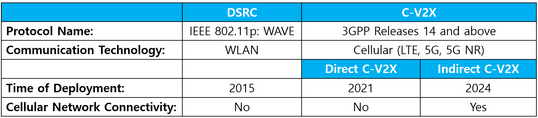
\includegraphics[width=0.6\linewidth]{image/DSRC} \caption{DSRC and C-V2X (Autocrypt, 2021)}\label{fig:unnamed-chunk-49}
\end{figure}

The term ``\emph{cellular}'' in C-V2X can cause some confusion. ``\emph{Cellular}'' in this context does not refer to the use of cellular networks, but to the use of the underlying electronics in cellular radios that are adapted to communicate directly from one radio to another. According to (Gettman, 2020), the following are the main similarities and differences between DSRC and C-V2X technology:

\textbf{Similarities}

\begin{itemize}
\tightlist
\item
  Both DSRC and C-V2X use the 5.9 Ghz band to communicate directly from one radio to another.
\item
  Both technologies use the same message sets (SAE J2735 and J2945) and use cases.
\item
  Both technologies use digital signatures to ensure security and trust in message providers.
\item
  In both cases, there is no link between radios. Each radio broadcasts the vehicle's location, speed, acceleration and other status elements while listening to other radios.
\end{itemize}

\textbf{Differences}

\begin{itemize}
\tightlist
\item
  DSRC uses a radio standard called WAVE, while C-V2X uses Long-Term Evolution (LTE) - the chip technology that almost all mobile phones use. A DSRC radio cannot talk to a C-V2X radio, and vice versa.
\item
  The range of DSRC is typically 300 m, and many installations have shown that a much higher range is possible. Initial tests of C-V2X show that the range is 20-30\% greater than DSRC and that performance in obstacles can be significantly improved. While C-V2X appears to have better performance initially, the range and reliability of DSRC is more than sufficient for the most important security applications.
\end{itemize}

Also relevant for wireless communications in the transport sector is VANET, a vehicular ad hoc network. It is a subclass of mobile ad hoc networks (MANETs), whereby it is developed by moving vehicles. VANET is increasingly known in the management of rush hour traffic congestion. The biggest challenge in VANET is the cooperation between nodes. In fact, even the best steering convention would not be beneficial if the hubs do not participate in sending the information (Rath et al., 2019).

\hypertarget{key-stakeholders-53}{%
\subsection*{Key stakeholders}\label{key-stakeholders-53}}
\addcontentsline{toc}{subsection}{Key stakeholders}

\begin{itemize}
\tightlist
\item
  \textbf{Affected}: Passenger vehicles drivers, Commercial vehicles drivers, Insurers
\item
  \textbf{Responsible}: National Governments, Technology companies, Car manufacturers, Infrastructure manufacturers
\end{itemize}

\hypertarget{current-state-of-art-in-research-53}{%
\subsection*{Current state of art in research}\label{current-state-of-art-in-research-53}}
\addcontentsline{toc}{subsection}{Current state of art in research}

Long before the creation of 5G, V2X communication was studied. Many analysts and people in the industry expect 5G to be the future technology for V2X communication due to the new speeds and other technical advances in 5G. Consequently, the security of 5G and how it can be integrated into the current ITS model needs to be studied extensively (Annu et al., 2021).

Some research investigates different materials and their properties for wireless communication (Nitika et al., 2021). There is also already some research being done on 6G antenna specifications for the next generation. The terahertz (THz) frequency band (0.1 - 10 THz) will be used in the 6G wireless communications system to support user demand for higher data rates and ultra-high-speed communications for many future applications (Hajiyat et al., 2021). Further, Zhao et al.~(2019) are testing a DSRC-based collision warning system because the accuracy of GPS is slightly affected by the driving environment, especially when shielded. Multi-sensor fusion positioning technology is a promising method to improve the accuracy of safety distance calculation and achieve lane-accurate positioning.

Mannoni et al.~(2019) compared TS-G5 and C-V2X for the V2X Communication Systems. C-V2X was showed to have better flexibility and performance than ITS-G5 at the same data rate. Based on the performance of the physical layer, the behaviour of both standards was evaluated in a network without mobile coverage and with multiple vehicles. Simulations showed that C-V2X performs better than ITS-G5 when the density of user is low. However, the performance of C-V2X deteriorates more than that of ITS-G5 when the level of congestion increases. The comparison of resource access time (latency) shows an advantage for ITS-G5, but the overall latency is not clearly better as it strongly depends on user density and coverage.

Findings of Sattiraju et al.~(2020) also show that C-V2X outperforms IEEE 802.11p DSRC (ITS-G5) technology for almost all of the channel models considered, with a gain of 0-5 dB. Furthermore, the results show that C-V2X performs better at higher vehicular speeds. This better performance of C-V2X can be attributed to the use of the turbo encoder and the better channel estimation mechanism that uses a higher number of DMRS symbols.

Salvo et al.~(2017) research on Heterogeneous cellular and DSRC networking for Floating Car Data collection in urban areas showed that it is reasonable to rely on direct V2V communication links (ITS-5G) before sending data over LTE channels (C-V2X). Their proposed solution fully adapts to the available penetration rate of VANET equipment; it automatically falls back to LTE-only FCD collection if VANET equipment is unavailable or too sparse. The achievable throughput of FCD collection is a key issue given the enormous amount of sensor data that can potentially be obtained from moving vehicles, e.g.~up to 100 Mbit/s can be transmitted on a vehicle's CAN bus (Kang et al., 2016). This extreme real-time and high-resolution Big Data requires new ideas for distributed processing and networking to pave the way for smart applications - a trend that has been little explored (Salvo et al., 2017).

\hypertarget{current-state-of-art-in-practice-53}{%
\subsection*{Current state of art in practice}\label{current-state-of-art-in-practice-53}}
\addcontentsline{toc}{subsection}{Current state of art in practice}

In Europe DSRC is the main technology currently in use. For example, in 2019, VW launched its Golf 8 with DSRC-based V2X. It made Europe's most popular car the first mass-market vehicle with V2X. In other parts of the world, after some large-scale field testing, DSRC-based V2X went into production in selected vehicle models in Japan in 2015 and in the US in 2017. While DSRC-based V2X is deployed in Europe and Japan, C-V2X is gaining momentum in other regions. China, for example, is driving the adoption of C-V2X. In early 2020, Autotalk's chipset was selected for a mass production C-V2X programme in China (Autotalks Ltd., n.d.).

DSRC and C-V2X run on different communication technologies and the access layer is not interoperable. This leaves car manufacturers and infrastructure developers with the difficult decision of whether to favour one technology or the other. However, many chip manufacturers are working on producing dual-mode chipsets that are compatible with both standards, making the switch easier for car manufacturers. As for infrastructure developers, many of them are working with existing DSRC infrastructures to add cellular network connectivity by combining them with indirect C-V2X. Regardless of the communication technologies used, cyber security is an integral part of V2X. AutoCrypt V2X is a security solution that embeds itself into V2X chipsets and protects the V2X system with both authentication and data encryption technologies (Autocrypt, 2021).

According to Erhart (2019) mobile radio (3G/4G, in future 5G) will be used in the long-distance sector. The C-ROADS initiative, in which 18 EU member states are working together on the subject of C-ITS, is endeavouring not only to harmonise and further develop C-ITS throughout Europe, but also to define the necessary interfaces and data formats for this long-distance solution in the mobile radio sector. ASFINAG is a leading member of the C-ROADS initiative in these areas and will take both types of communication into account in the implementation.

The next generation of the communication technology could be initiated by companies such as Starlink or Kuiper if they are successful in deploying LEO constellations (Techbook, 2020). Starlink is a sub-company of Spacex and is trying to build an interconnected Internet network with thousands of satellites to deliver high-speed internet around the world (Sheetz, 2021). Starlink satellites are more than 60 times closer to Earth than conventional satellites, resulting in lower latency. Starlink is ideally suited for areas of the world where connectivity is normally a challenge (Starlink, n.d.). However, densely populated urban areas pose a problem (Holland, 2021). There are currently 1100 SpaceX satellites in space to build the global Internet service. Several thousand more satellites are to be added in the coming years. As ``\emph{Golem}'' reports, there are to be 12000 satellites in the full expansion stage (finanzen.net, 2021). Starlink has already received more than 500.-000 orders for its satellite Internet service. While competitors like OneWeb or Amazon's Project Kuiper are lagging behind, SpaceX is creating more and more facts with Starlink (Holland, 2021). However, satellite Internet is intended for aircraft, ships, large trucks and motor homes. They are not yet suitable for passenger cars, as they are simply far too large for this (Musk, 2021).

Further, researchers warn of some consequences for astronomy due to this satellite system. The disadvantages include shorter effective working time of telescopes (due to satellites that may be in between during observations in space), higher potential for collision with research infrastructure, production of debris in orbit, increased need for costly evasive manoeuvres of spaceships during space missions (Traxler \& Rennert, 2020).

\hypertarget{relevant-initiatives-in-austria-53}{%
\subsection*{Relevant initiatives in Austria}\label{relevant-initiatives-in-austria-53}}
\addcontentsline{toc}{subsection}{Relevant initiatives in Austria}

DSRC modules are already used for truck toll billing in Austria. Around 152000 vehicles generated around 190 million euros in toll revenue in Austria via the Toll Collect OBU in 2018. The DSRC module works on a microwave basis and triggers a toll transaction when the vehicle passes through a toll collection station on Austrian motorways and motorways, which is then transmitted from the toll collection station to ASFINAG's data centre for billing. The Toll Collect On-Board Unit, which is permanently installed in the truck, is characterised by high availability and stability. In Germany, the OBU continues to collect tolls via satellite.

\begin{itemize}
\tightlist
\item
  \href{https://www.toll-collect.de/de/toll_collect/unternehmen/presse/pressemitteilungen/detailseite_press_6241.html}{Toll-collect.de}
\end{itemize}

Another current application of DSRC is the remote retrieval of tachograph data by control authorities. Since 15 June 2019, it has been mandatory to equip new trucks and buses over 3.5t MPTW (maximum permissible total weight) with a ``smart tacho'' that enables this (WKÖ, 2019). There are currently two C-ITS test environments: one around Vienna and one near Graz. The plan is to expand from 2020 onwards. The first area to be covered will be the Salzburg - Vienna corridor, the A2 around Graz and selected border areas.

At the European level, a community of road operators, vehicle and agricultural machinery manufacturers, cities, as well as industrial and telecom companies have come together to form an interest group called the ``\emph{C-ITS Deployment Group}''. The members of this group are committed to a coordinated C-ITS deployment in Europe, that is, C-ITS services should look the same across Europe and be understood by all vehicles (Erhart, 2019).

\begin{itemize}
\tightlist
\item
  \href{https://blog.asfinag.at/technik-innovation/c-its-vernetzte-autos-intelligenter-verkehr/}{Asfinag.at}
\end{itemize}

\hypertarget{impacts-with-respect-to-sustainable-development-goals-sdgs-53}{%
\subsection*{Impacts with respect to Sustainable Development Goals (SDGs)}\label{impacts-with-respect-to-sustainable-development-goals-sdgs-53}}
\addcontentsline{toc}{subsection}{Impacts with respect to Sustainable Development Goals (SDGs)}

\begin{longtable}[]{@{}
  >{\centering\arraybackslash}p{(\columnwidth - 8\tabcolsep) * \real{0.2029}}
  >{\centering\arraybackslash}p{(\columnwidth - 8\tabcolsep) * \real{0.1884}}
  >{\centering\arraybackslash}p{(\columnwidth - 8\tabcolsep) * \real{0.2029}}
  >{\centering\arraybackslash}p{(\columnwidth - 8\tabcolsep) * \real{0.2029}}
  >{\centering\arraybackslash}p{(\columnwidth - 8\tabcolsep) * \real{0.2029}}@{}}
\toprule()
\begin{minipage}[b]{\linewidth}\centering
Impact level
\end{minipage} & \begin{minipage}[b]{\linewidth}\centering
Indicator
\end{minipage} & \begin{minipage}[b]{\linewidth}\centering
Impact direction
\end{minipage} & \begin{minipage}[b]{\linewidth}\centering
Goal description and number
\end{minipage} & \begin{minipage}[b]{\linewidth}\centering
Source
\end{minipage} \\
\midrule()
\endhead
Systemic & Continuous development of communication technologies & \textbf{+} & Innovation \& Infrastructure (\emph{9}) & Techbook, 2020; Autotalks Ltd., n.d.; Salvo et al., 2017 \\
Systemic & New initiatives and interest groups are created & \textbf{+} & Partnership \& collaborations (\emph{17}) & Erhart, 2019 \\
\bottomrule()
\end{longtable}

\hypertarget{technology-and-societal-readiness-level-53}{%
\subsection*{Technology and societal readiness level}\label{technology-and-societal-readiness-level-53}}
\addcontentsline{toc}{subsection}{Technology and societal readiness level}

\begin{longtable}[]{@{}cc@{}}
\toprule()
TRL & SRL \\
\midrule()
\endhead
5-8 & 6-8 \\
\bottomrule()
\end{longtable}

\hypertarget{open-questions-51}{%
\subsection*{Open questions}\label{open-questions-51}}
\addcontentsline{toc}{subsection}{Open questions}

1.What are the alternative solutions for joining DSRC and C-V2X so that they are compatible with one another?

\hypertarget{further-links-45}{%
\subsection*{Further links}\label{further-links-45}}
\addcontentsline{toc}{subsection}{Further links}

\begin{itemize}
\tightlist
\item
  \href{https://c-its-korridor.de/?menuId=1\&sp=en}{C-its-korridor.de}
\item
  \href{https://www.asfinag.at/ueber-uns/newsroom/pressemeldungen/2020/wlan-ausbau-cooperative-intelligent-transport-systems/}{Asfinag.at}
\item
  \href{https://www.autocrypt.io/blog-post/dsrc-vs-c-v2x-detailed-comparison}{Autocrypt.io}
\item
  \href{https://www.kimley-horn.com/news-insights/dsrc-cv2x-comparison-future-connected-vehicles/}{Kimley-horn.com}
\end{itemize}

\hypertarget{references-53}{%
\subsection*{References}\label{references-53}}
\addcontentsline{toc}{subsection}{References}

\begin{itemize}
\tightlist
\item
  Annu, Kaushik, D., \& Gupta, A. (2021). Ultra-secure transmissions for 5G-V2X communications. Materials Today: Proceedings. \url{https://doi.org/10.1016/j.matpr.2020.12.130}
\item
  Autocrypt. (2021). AUTOCRYPT - DSRC vs.~C-V2X: A Detailed Comparison of the 2 Types of V2X Technologies. \url{https://www.autocrypt.io/blog-post/dsrc-vs-c-v2x-detailed-comparison}
\item
  Autotalks Ltd.~(n.d.). C-V2X vs DSRC \textbar{} Get Your Facts Straight on Cellular V2X, LTE-V and LTE-V2X Autotalks. Available at: \url{https://www.auto-talks.com/technology/dsrc-vs-c-v2x-2/} {[}Accessed: 4 May 2021{]}
\item
  Erhart, J. (2019, November 28). Vernetzte Autos, intelligenter Verkehr: Was C-ITS ist, was es kann und wem es nutzt.Available at: \url{https://blog.asfinag.at/technik-innovation/c-its-vernetzte-autos-intelligenter-verkehr/} {[}Accessed: 4 May 2021{]}
\item
  Fillenberg, S. (2017, December 18). Cellular V2X: Continental Successfully Conducts Field Trials in China. Continental Press Release. \url{https://www.continental.com/en/press/press-releases/2017-12-18-cellular-v2x-116994}
\item
  finanzen.net. (2021, May 5). Internet aus dem All: Internetsparte von SpaceX: Starlink bald in Wohnmobilen, Schiffen und Flugzeugen? \textbar{} Nachricht \textbar{} finanzen.net. \url{https://www.finanzen.net/nachricht/geld-karriere-lifestyle/internet-aus-dem-all-internetsparte-von-spacex-starlink-bald-in-wohnmobilen-schiffen-und-flugzeugen-9905140}
\item
  Gettman, D. (2020, June 3). DSRC and C-V2X: The Future of Connected Vehicles \textbar{} Kimley-Horn. \url{https://www.kimley-horn.com/news-insights/dsrc-cv2x-comparison-future-connected-vehicles/}
\item
  Hajiyat, Z. R. M., Ismail, A., Sali, A., \& Hamidon, M. N. (2021). Antenna in 6G wireless communication system: Specifications, challenges, and research directions. Optik, 231(February), 166415. \url{https://doi.org/10.1016/j.ijleo.2021.166415}
\item
  Holland, M. (2021, May 5). Starlink: Schon 500.000 Vorbestellungen für Satelliten-Internet von SpaceX \textbar{} heise online. \url{https://www.heise.de/news/Starlink-Schon-500-000-Vorbestellungen-fuer-Satelliten-Internet-von-SpaceX-6036732.html}
\item
  IEEE. (2014). IEEE Guide for Wireless Access in Vehicular Environments (WAVE) - Architecture. IEEE Std 1609.0-2013, 1--78. \url{https://doi.org/10.1109/IEEESTD.2014.6755433}
\item
  Kang, S., Han, S., Cho, S., Jang, D., Choi, H., \& Choi, J.-W. (2016). High speed CAN transmission scheme supporting data rate of over 100 Mb/s. IEEE Communications Magazine, 54(6), 128--135. \url{https://doi.org/10.1109/MCOM.2016.7498099}
\item
  Mannoni, V., Berg, V., Sesia, S., \& Perraud, E. (2019). A comparison of the V2X communication systems: ITS-G5 and C-V2X. IEEE Vehicular Technology Conference, 2019-April. \url{https://doi.org/10.1109/VTCSpring.2019.8746562}
\item
  Musk, E. (2021, March 7). Elon Musk auf Twitter. \url{https://twitter.com/elonmusk/status/1369051431903268865?ref_src=twsrc\%5Etfw\%7Ctwcamp\%5Etweetembed\%7Ctwterm\%5E1369051431903268865\%7Ctwgr\%5E\%7Ctwcon\%5Es1}
\item
  Nitika, Rana, A., Kumar, V., \& Awasthi, A. M. (2021). Effect of dopant concentration and annealing temperature on electric and magnetic properties of lanthanum substituted CoFe2O4 nanoparticles for potential use in 5G wireless communication systems. Ceramics International. \url{https://doi.org/10.1016/j.ceramint.2021.04.077}
\item
  Rath, M., Pati, B., \& Pattanayak, B. K. (2019). An Overview on Social Networking: Design, Issues, Emerging Trends, and Security. In Social Network Analytics (pp.~21--47). Elsevier. \url{https://doi.org/10.1016/b978-0-12-815458-8.00002-5}
\item
  Salvo, P., Turcanu, I., Cuomo, F., Baiocchi, A., \& Rubin, I. (2017). Heterogeneous cellular and DSRC networking for Floating Car Data collection in urban areas. Vehicular Communications, 8, 21--34. \url{https://doi.org/10.1016/j.vehcom.2016.11.004}
\item
  Sattiraju, R., Wang, D., Weinand, A., \& Schotten, H. D. (2020). Link level performance comparison of C-V2X and ITS-G5 for vehicular channel models. ArXiv, March.
\item
  Sheetz, M. (2021, May 4). SpaceX: Over 500,000 orders for Starlink satellite internet service. Available at: \url{https://www.cnbc.com/2021/05/04/spacex-over-500000-orders-for-starlink-satellite-internet-service.html} {[}Accessed: 4 May 2021{]}
\item
  Starlink. (n.d.). Starlink. Available at: \url{https://www.starlink.com/} {[}Accessed: 6 May 2021{]}
\item
  Techbook. (2020, November 16). LTE, 4G und 5G: Die Unterschiede zwischen den Mobilfunkstandards.Available at: \url{https://www.techbook.de/mobile/lte-4g-unterschied-mobil-smartphone} {[}Accessed: 4 May 2021{]}
\item
  Traxler, T., \& Rennert, D. (2020, February 17). Starlink: Elon Musks Satellitenflotte in der Kritik - Raum - derStandard.at › Wissenschaft.Available at: \url{https://www.derstandard.at/story/2000114681438/starlink-elon-musks-satellitenflotte-in-der-kritik} {[}Accessed: 4 May 2021{]}
\item
  WKÖ. (2019). Ausrüstungspflicht von neuen lkw und omnibussen mit einem „smart tacho`` ab 15. Juni 2019. Available at: \url{https://www.google.com/url?sa=t\&rct=j\&q=\&esrc=s\&source=web\&cd=\&ved=2ahUKEwiyka_Xs7XwAhXytYsKHTq_AJ0QFjADegQIBBAD\&url=https\%3A\%2F\%2Fwww.wko.at\%2Fbranchen\%2Ftransport-verkehr\%2Fausruestungspflicht-smart-tacho.pdf\&usg=AOvVaw12-xLPvw33KN9gvYKy51tn} {[}Accessed: 4 May 2021{]}
\item
  Zhao, X., Jing, S., Hui, F., Liu, R., \& Khattak, A. J. (2019). DSRC-based rear-end collision warning system -- An error-component safety distance model and field test. Transportation Research Part C: Emerging Technologies, 107, 92--104. \url{https://doi.org/10.1016/j.trc.2019.08.002}
\end{itemize}

\hypertarget{bd_life}{%
\section{Big data lifecycle}\label{bd_life}}

\hypertarget{definition-54}{%
\subsection*{Definition}\label{definition-54}}
\addcontentsline{toc}{subsection}{Definition}

``\emph{Big Data refers to large data sets that include heterogeneous formats: structured, unstructured and semi-structured data. Big Data has a complex nature that require powerful technologies and advanced algorithms. So the traditional static Business Intelligence tools can no longer be efficient in the case of Big Data applications}'' (Oussous et al., 2018). It is typically characterized by 3Vs (volume, velocity and variety) as described in \protect\hyperlink{bd_tool_maping}{Big Data Tools} topic. In transport context the major sources of Big Data are:

\begin{itemize}
\tightlist
\item
  Drivers' assistance systems and instrumented vehicles which constantly monitor the vehicle surroundings and driving behaviour
  Yuan et al.~(2015) claims that connected vehicles could produce even 30 GB of data per day.
\item
  Traveller information systems
\item
  Roadway operations and management such as \protect\hyperlink{variable_speed}{variable speed limits and dynamic signage system}
\item
  Traffic data
  For example, \protect\hyperlink{traffic_info_monitoring}{real-time traffic information and monitoring} which can produce structured and unstructured data, such as JPG, JSON, GPS, PDF, image, video, and social media posts (Kemp et al., 2015)
\item
  Emergency and incident management
\end{itemize}

The literature summarised in Neilson et al.~(2019) shows the following use of Big Data in transport context:

\begin{longtable}[]{@{}
  >{\centering\arraybackslash}p{(\columnwidth - 6\tabcolsep) * \real{0.2500}}
  >{\centering\arraybackslash}p{(\columnwidth - 6\tabcolsep) * \real{0.2500}}
  >{\centering\arraybackslash}p{(\columnwidth - 6\tabcolsep) * \real{0.2500}}
  >{\centering\arraybackslash}p{(\columnwidth - 6\tabcolsep) * \real{0.2500}}@{}}
\toprule()
\begin{minipage}[b]{\linewidth}\centering
Big Data systems used
\end{minipage} & \begin{minipage}[b]{\linewidth}\centering
Purposes of Big Data analysis
\end{minipage} & \begin{minipage}[b]{\linewidth}\centering
Types of data collected
\end{minipage} & \begin{minipage}[b]{\linewidth}\centering
Current opportunities and challenges
\end{minipage} \\
\midrule()
\endhead
ITS, Hadoop, MapReduce, batch and stream data processing, NoSQL & urban planning, collision and near miss analysis, traffic congestion, safety, optimization & Speed, location, video, image, traffic intensity, social media, crowdsourcing, machine learning, historical, real-time, predictive, visual, video/image analytics & Data collection, quality, storage, processing, privacy, security, connected and autonomous vehicle \\
\bottomrule()
\end{longtable}

Further, an important part of Big Data is its life cycle, also called the information life cycle which is defined as the period of time that the data exists in the system. This life cycle encompasses all the stages that the data goes through, from first capture onward (Talend.com, 2021). Current literature proposes different models depending on the nature of the data and specific field. Nonetheless, they display some similarities and the majority of phases are shared by most data cycle models. For instance, according to Arras \& Souissi (2018) the key phases of Big Data Lifecycle are:

\begin{itemize}
\tightlist
\item
  \emph{Planning}: A detailed description of how data will be used, managed and made accessible throughout their life cycle
\item
  \emph{Management}: Includes all the operational phases that directly manipulate the data
\item
  \emph{Collection}: It consists of receiving the raw data of different types and making the conversions and modifications necessary to organize them. Cleaning of data received in real-time saves calculation time and memory space. Data quality must be carried out at this level because it makes it possible to optimize the data processing circuit overall
\item
  \emph{Integration}: The purpose of this phase is to provide a coherent pattern of data from multiple independent, distributed and
  heterogeneous sources of information so as to facilitate users accessing and querying such data as if they were accessing only one data source
\item
  \emph{Filtering}: Consists in restricting the large data flow to remove irrelevant data or errors
\item
  \emph{Enrichment}: Data enrichment involves making structural or hierarchical changes to received data. It allows adding information on collected data to improve their quality
\item
  \emph{Analysis}: In this phase, the data is exploited and analysed to draw conclusions and interpretations of decision-making
\item
  \emph{Access}: This phase is focused on the communication/interaction with the data consumer
\item
  \emph{Visualisation}: It consists of displaying the results of the analysis in a concise way so that decision-makers can easily understand these results and make informed decisions
\item
  \emph{Storage}: Concerns all the other phases of the cycle and makes it possible to store the data throughout its life cycle in order to
  have a continuous traceability of data in each phase of the cycle
\item
  \emph{Destruction}: In this phase data is discarded when it is successfully used and will become useless and without added value
\item
  \emph{Archiving}: Consists of an implementation of data security and confidentiality
\end{itemize}

Further, Djahel et al., (2014) proposed big data life cycle with respect to traffic management systems (TMS) as visualised in Figure 12.2.

\begin{figure}
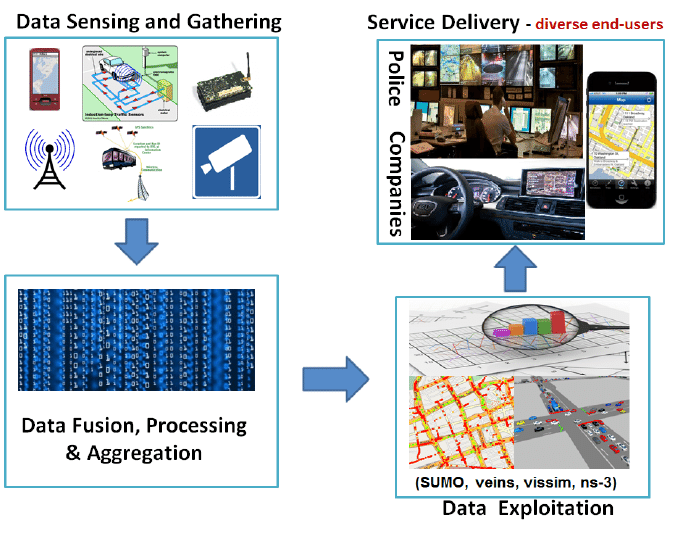
\includegraphics[width=0.75\linewidth]{image/BDLC} \caption{Big Data lifecycle in smart transportation (Djahel et al., 2014)}\label{fig:unnamed-chunk-51}
\end{figure}

In the first phase \emph{Data Sensing and Gathering (DSG)} the traffic data is monitored and collected, providing information about traffic volumes, incidents, occupancy or speed. Gathered data later feeds into the second phase \emph{Data Fusion, Processing and Aggregation} where the relevant information is extracted from raw data. Next, in the third phase \emph{Data Exploitation} the processed data is used to compute optimal routes, provide forcasts and obtain traffic statistics. Lastly, in the \emph{Service Delivery} phase, the TMS shares the knowledge with the end users such as drivers, authorities or passengers through the variety of
devices such as smart phones or vehicles' on-board units.

\hypertarget{key-stakeholders-54}{%
\subsection*{Key stakeholders}\label{key-stakeholders-54}}
\addcontentsline{toc}{subsection}{Key stakeholders}

\begin{itemize}
\tightlist
\item
  \textbf{Affected}: Passengers, Drivers, ITS focused companies
\item
  \textbf{Responsible}: National Governments, Technology companies, ITS focused companies, Transport operators, Transport software developers
\end{itemize}

\hypertarget{current-state-of-art-in-research-54}{%
\subsection*{Current state of art in research}\label{current-state-of-art-in-research-54}}
\addcontentsline{toc}{subsection}{Current state of art in research}

As mentioned above, literature offers different models of Big Data life cycle, beyond the Smart Data Lifecycle (DLC) model proposed by
Arras \& Souissi (2018). For example, according to Alshboul et al.~(2015) the life cycle of Big Data encompasses four phases:

\begin{itemize}
\tightlist
\item
  \emph{Data collection}
  Data from different sources comes with different formats: structured, semi-structured, and unstructured.
\item
  \emph{Data storage}
  The collected data is stored and prepared for being used in the next phase. As the collected data may contain of sensitive information, it is essential to take sufficient precautions (e.g.~permutation, anonimisation) during data storing.
\item
  \emph{Data analytics}
  Data is analysed to generate useful knowledge. In this phase, data mining methods such as clustering, classification, and
  association rule mining are used.
\item
  \emph{Knowledge creation }
  The results of the analyses are used by the decision makers.
\end{itemize}

While Demchenko et al.~(2014) proposes Big Data Lifecycle Management (BDLM) model that consists of six stages:

\begin{itemize}
\tightlist
\item
  Data source
\item
  Data collection
\item
  Data cleaning (filtering, classification)
\item
  Data analytics
\item
  Data visualisations
\item
  Data analytics application
\end{itemize}

\hypertarget{current-state-of-art-in-practice-54}{%
\subsection*{Current state of art in practice}\label{current-state-of-art-in-practice-54}}
\addcontentsline{toc}{subsection}{Current state of art in practice}

The typical management tools, techniques and software used to handle data are Google BigTable, Simple DB, Not Only SQL (NoSQL), Data Stream Management System (DSMS), MemcacheDB and Voldemort. However, new applications with higher capabilities are continuously developed to match Big Data requirements (Chen et al., 2014). For example, \href{https://hadoop.apache.org/}{Hadoop} is specifically designed to manage Big Data at different stages of its life cycle. It is an open source software framework that allows for the processing of large data sets across clusters of computers using simple programming models such as Google MapReduce (Khan et al., 2014). Hadoop can process extremely large volumes of data with varying structures (or no structure at all). It is typically applied to large amounts of data, enabling to handle data that was previously difficult to manage and analyse.

In terms of real-life examples, big data together with the Internet of Things (IoT) are used by Data Mill North's national public transport access nodes (NaPTAN) in the UK to provide real-time transport information to passengers. For instance, train operators have been already using Big Data to offer information on live seat availability (Rayner, 2017).

\hypertarget{relevant-initiatives-in-austria-54}{%
\subsection*{Relevant initiatives in Austria}\label{relevant-initiatives-in-austria-54}}
\addcontentsline{toc}{subsection}{Relevant initiatives in Austria}

\begin{itemize}
\tightlist
\item
  \href{https://confare.at/wiener-linien-digitale-zukunft/}{Wiener Linien}
\end{itemize}

\hypertarget{impacts-with-respect-to-sustainable-development-goals-sdgs-54}{%
\subsection*{Impacts with respect to Sustainable Development Goals (SDGs)}\label{impacts-with-respect-to-sustainable-development-goals-sdgs-54}}
\addcontentsline{toc}{subsection}{Impacts with respect to Sustainable Development Goals (SDGs)}

\begin{longtable}[]{@{}
  >{\centering\arraybackslash}p{(\columnwidth - 8\tabcolsep) * \real{0.2029}}
  >{\centering\arraybackslash}p{(\columnwidth - 8\tabcolsep) * \real{0.1884}}
  >{\centering\arraybackslash}p{(\columnwidth - 8\tabcolsep) * \real{0.2029}}
  >{\centering\arraybackslash}p{(\columnwidth - 8\tabcolsep) * \real{0.2029}}
  >{\centering\arraybackslash}p{(\columnwidth - 8\tabcolsep) * \real{0.2029}}@{}}
\toprule()
\begin{minipage}[b]{\linewidth}\centering
Impact level
\end{minipage} & \begin{minipage}[b]{\linewidth}\centering
Indicator
\end{minipage} & \begin{minipage}[b]{\linewidth}\centering
Impact direction
\end{minipage} & \begin{minipage}[b]{\linewidth}\centering
Goal description and number
\end{minipage} & \begin{minipage}[b]{\linewidth}\centering
Source
\end{minipage} \\
\midrule()
\endhead
Systemic & Increased safety of drivers and public transport passengers & \textbf{+} & Health \& Wellbeing (\emph{3}) & Rayner, 2017 \\
Systemic & Increased energy consumption & \textbf{-} & Environmental sustainability (\emph{7,12-13,15}) & Lovell, 2018 \\
Systemic & Potential for more reliable and transparent partnership along the supply chain & \textbf{+} & Partnership \& collaborations (\emph{17}) & Robins, 2021 \\
\bottomrule()
\end{longtable}

\hypertarget{technology-and-societal-readiness-level-54}{%
\subsection*{Technology and societal readiness level}\label{technology-and-societal-readiness-level-54}}
\addcontentsline{toc}{subsection}{Technology and societal readiness level}

\begin{longtable}[]{@{}cc@{}}
\toprule()
TRL & SRL \\
\midrule()
\endhead
5-9 & 6-9 \\
\bottomrule()
\end{longtable}

\hypertarget{open-questions-52}{%
\subsection*{Open questions}\label{open-questions-52}}
\addcontentsline{toc}{subsection}{Open questions}

\begin{enumerate}
\def\labelenumi{\arabic{enumi}.}
\tightlist
\item
  How to reduced potential for cyber-attacks and how the security methods can be improved?
\item
  How can the problem of seeing data as a threat, in German speaking countries, be alleviated?
\end{enumerate}

\hypertarget{references-54}{%
\subsection*{References}\label{references-54}}
\addcontentsline{toc}{subsection}{References}

\begin{itemize}
\tightlist
\item
  Alshboul, Y., Nepali, R. K., \& Wang, Y. (2015, August). Big Data LifeCycle: Threats and Security Model. In AMCIS.
\item
  Chen, M., Mao, S., \& Liu, Y. (2014). Big data: A survey. Mobile networks and applications, 19(2), 171-209.
\item
  Demchenko, Y., De Laat, C., \& Membrey, P. (2014, May). Defining architecture components of the Big Data Ecosystem. In 2014 International conference on collaboration technologies and systems (CTS) (pp.~104-112). IEEE.
\item
  Djahel, S., Doolan, R., Muntean, G. M., \& Murphy, J. (2014). A communications-oriented perspective on traffic management systems for smart cities: Challenges and innovative approaches. IEEE Communications Surveys \& Tutorials, 17(1), 125-151.
\item
  El Arass, M., \& Souissi, N. (2018, October). Data lifecycle: From big data to smartdata. In 2018 IEEE 5th international congress on information science and technology (CiSt) (pp.~80-87). IEEE.
\item
  Kemp, G., Vargas-Solar, G., Da Silva, C. F., \& Ghodous, P. (2015, May). Aggregating and managing big realtime data in the cloud-application to intelligent transport for smart cities. In Proceedings of the 1st international conference on vehicle technology and intelligent transport systems (pp.~107-112).
\item
  Khan, N., Yaqoob, I., Hashem, I. A. T., Inayat, Z., Mahmoud Ali, W. K., Alam, M., \ldots{} \& Gani, A. (2014). Big data: survey, technologies, opportunities, and challenges. The scientific world journal, 2014.
\item
  Neilson, A., Daniel, B., \& Tjandra, S. (2019). Systematic review of the literature on big data in the transportation domain: Concepts and applications. Big Data Research, 17, 35-44.
\item
  Oussous, A., Benjelloun, F. Z., Lahcen, A. A., \& Belfkih, S. (2018). Big Data technologies: A survey. Journal of King Saud University-Computer and Information Sciences, 30(4), 431-448.
  Rayner, T. (2017). Deriving Transport Benefits from Big Data and the Internet of Things in Smart Cities. Available at: \url{https://www.womblebonddickinson.com/uk/insights/articles-and-briefings/deriving-transport-benefits-big-data-and-internet-things-smart} {[}Accessed: 12 August 2021{]}
\item
  Robins, C. (2021). WHY BIG DATA IS SO IMPORTANT TO THE TRANSPORTATION INDUSTRY Available at: \url{https://www.robinsconsulting.com/why-big-data-is-so-important/} {[}Accessed: 12 August 2021{]}
\item
  Talend.com (2021). Data Lifecycle Management (Definition and Framework). Available at: \url{https://www.talend.com/resources/data-lifecycle-management/} {[}Accessed: 12 August 2021{]}.
\item
  Yuan, W., Deng, P., Taleb, T., Wan, J., \& Bi, C. (2015). An unlicensed taxi identification model based on big data analysis. IEEE Transactions on Intelligent Transportation Systems, 17(6), 1703-1713.
\end{itemize}

\hypertarget{bd_tool_maping}{%
\section{Big data tools for mapping and forecasting travel behaviour}\label{bd_tool_maping}}

\hypertarget{synonyms-49}{%
\subsection*{Synonyms}\label{synonyms-49}}
\addcontentsline{toc}{subsection}{Synonyms}

\emph{application programming interface (API)}

\hypertarget{definition-55}{%
\subsection*{Definition}\label{definition-55}}
\addcontentsline{toc}{subsection}{Definition}

\textbf{(Real Time) Traffic mapping}
Traffic mapping is accomplished on the one hand with traffic sensors and on the other hand with smartphone data. State transport departments have started installing solar-powered traffic sensors on major roads across the country to record the current traffic situation in order to collect planning statistics, improve accident response times and increase traffic flow.
The data is collected using different types of traffic sensors. In recent years, three above-ground types have become popular: radar, active infrared and laser radar. Radar sensor technology has been around since World War II, when it helped the military track enemy ships in the air and at sea. Today's technology allows each of these devices to monitor multiple lanes of traffic simultaneously (Machay, n.d.).

Google Maps is a major player in the field of navigation and traffic mapping. Until March 2012, there was no traffic feature - they simply focused on getting people from point A to point B. There was a feature before that showed how much traffic would slow a driver down, but there was no live data. Back then, only historical data was used to show how long the same route would take ``in heavy traffic'' (NCTA, 2013).

Then, on one hand, an agreement was reached with the traffic authorities to share the data generated by the sensors, and on the other hand, smartphone data could be used for real-time data. The data from the traffic authorities' traffic sensors enabled Google to expand its traffic services, while the traffic authorities were able to pay part of the costs for the sensors. By working with various traffic authorities, Google received up-to-date information about congestion on motorways and major roads but was hardly able to monitor traffic on smaller rural roads and in residential areas. Current traffic data is collected mainly via GPS-enabled mobile phones running the Google Maps application. This continuously transmits the location and speed of each user to Google in real time. Using a technique known as ``crowdsourcing'', Google combines the information provided by thousands of active mobile phones to determine how fast traffic is moving in a given location (Machay, n.d.). Regarding privacy, Google claims that users can decide whether or not to share their travel data with Google in their phone's settings. The company points out that it tries to protect the information (Google itself doesn't even know what data comes from which car, and it cuts off the first and last minutes of each trip to further obscure it). If users opt in, they help providing a helpful service - users get more realistic estimates of how long their journey will take and are better prepared for traffic. Mike Dobson (president of Telemapics) envisions a future scenario in which Google could suggest reroutes to 5 \% of users to either ease traffic congestion or reduce the probability of delays occurring in the first place. Zhan Guo, a transportation policy professor at New York University, says it will be difficult to give advice on how to reroute traffic because drivers who travel a route daily know best what will take the longest. If there are few other ways to get from A to B, it's pointless to suggest alternatives, because everyone will rush to clog up another road. An algorithm that diverts just the right amount of traffic is probably still a few years away, he says (NCTA, 2013).

Due to the increasing prevalence of mobile phones with built-in location and motion sensors in the population, extensive and dynamic data can be collected. Mobile phone data enables unprecedented population and geographic area coverage (Wang et al., 2018).
The disadvantages of these systems are that radar sensors cannot detect broken-down vehicles because they cannot detect objects that are not moving. Active infrared and laser radar sensors do not work properly in dense fog or blowing snow. And crowdsourcing accuracy can be compromised if not enough mobile phones provide data for a given area (Machay, n.d.).

\textbf{Traffic forecasting}
In order to forecast traffic demand, information about the past, the state of the transport system and its external system are considered. Traffic forecasting methods can be divided into different types according to mathematical methods and calculation procedures, such as qualitative and quantitative, linear and nonlinear, dynamic and static, aggregated and disaggregated (Zhao et al., 2018).

Since the 1950s, the ``four-stage model'' has dominated travel demand forecasting methods. Since the 1970s, activity-based forecasting methods have attracted more attention.

\textbf{Trip-based forecasting methods}
Trip-based travel demand forecasting methods usually subdivide the unit of travel forecast in terms of an ``aggregate'' (traffic zone) and focus on the population and land use of the traffic zone. These methods generally consider spatial coordination at the city level, but ignore the actual travel needs and feelings of individual residents. Therefore, due to the low flexibility and low refinement level of the prediction results, these methods can easily lead to problems with uneven traffic distribution (Qin et al., 2013).

There are several travel-based forecasting methods. Zhao et al.~(2018) lists 5 basic ones with advantages and limitations:

\begin{itemize}
\tightlist
\item
  Gray System Theory (GST)
  In this system, some information is known and some information is unknown. It is almost impossible to use for short term forecasting based on conventional survey data.
\item
  Kalman filtering (KF)
  It can estimate the state of the dynamic system from a set of incomplete and noisy measurements.
\item
  Chaos Theory (CT)
  This focuses on the ordered structure and regularity of seemingly random phenomena in dynamical systems. However, a large amount of traffic monitoring data is required as training or decision samples. Due to data acquisition, input, transmission, and storage, these methods require lengthy preprocessing of the data and have limited real-time capabilities.
\item
  Artificial Neural Network (ANN)
  A mathematical model that mimics the structure and function of biological neural networks. This also requires large amounts of traffic monitoring data and lengthy preprocessing of the data.
\item
  Support Vector Machine (SVM)
  A machine learning method.
\end{itemize}

\textbf{Activity-based forecasting methods}
Activity-based forecasting methods are a type of disaggregated forecasting methods that focus on the reasons for individuals' travel and the ``activity-travel'' model, using individuals as the research subjects. These methods also study the causal relationship between activities and travel. Examples include the multi-agent system (MAS) model and the multinomial logit (MNL) model. Activity-based forecasting requires a large amount of individual sample data (Zhao et al., 2018). Due to limited data processing capacity, they are primarily used for mode split and rarely used for traffic generation and distribution forecasting (P. Wang et al., 2013).

\textbf{Big Data}
Big Data refers to data that, at a certain stage of development, can no longer be collected, stored, analysed, or processed using traditional database software tools (Manyika et al., 2011). There are some characteristics and features of Big Data that are referred to as the Vs of Big Data Management (Al Nuaimi et al., 2015). According to Fan \& Bifet (2013), these include the 3 main Vs (1, 2 and 3) and two other Vs:

\begin{itemize}
\tightlist
\item
  Volume: refers to the size of data created from all sources.
\item
  Velocity: refers to the speed at which data is created, stored, analysed and processed.
\item
  Variety: refers to the different types of data that are generated. It is common today for most data to be unstructured and not easily categorised or tabulated.
\item
  Variability: refers to the fact that the structure and meaning of the data is constantly changing, especially in the case of data derived from, for example, natural language analysis.
\item
  Value: refers to the potential advantage that Big Data can provide to a company based on good collection, management and analysis of Big Data.
\end{itemize}

Others mention some more Vs of Big Data, covering some more aspects. For example, volatility, which refers to the retention policy of structured data from different sources. Validity refers to the correctness, accuracy and validation of the data. Veracity refers to the accuracy and truthfulness of the data collected and the meaningfulness of the results generated from the data for specific problems (Al Nuaimi et al., 2015).

Other unique characteristics compared to traditional data analysis methods are: (1) the data source is extended from the sample data to the whole data; (2) the data of a single domain is extended to the cross-domain data; (3) the Big Data analysis mainly explores the relationships between the data (Zhao et al., 2018).

Due to the advancement of various technologies, the volume, variety and availability of data has increased rapidly. By 2003, humanity had generated five exabytes (5 × 106 terabytes) of data (Sagiroglu \& Sinanc, 2013). The same amount of data was generated in just two days in 2012 (McAfee et al., 2012).

In the past, road safety research studies have mostly used manually collected data (e.g.~data from handwritten police accident reports) together with estimated static traffic volumes. Installations of detectors, sensors, a rapid spread of ITS and the advent of CAV led to an increase in the amount of data on people, vehicles, roads and environments (Lian et al., 2020).

Historically, travel behaviour research data has largely been derived from travel surveys, and such data is costly to collect and outdated. This has limited data collection and inhibited progress in travel behaviour research (Liu et al., 2016). In the era of Big Data, various new data sources can be used to supplement or replace traditional survey data to support travel behaviour research. Some examples are data from smart card records, GPS-based taxi trajectory data and roadside sensor data, with mobile phone data being the most common and promising type (Yue et al., 2014). There are two main sources of mobile phone data currently used for travel behaviour research (Z. Wang et al., 2018):

\begin{itemize}
\tightlist
\item
  Mobile phone network data
  This involves using RF (radio frequency) signals to determine the location of mobile phones. These RF signals include mobile network signals, GPS, AGPS, WiFi and Bluetooth.
\item
  Smartphone sensor data
  Built-in sensors (accelerometers, magnetic sensors and compasses) are used to monitor the movement status of mobile phones.
  Different types of data are collected by different organisations using different techniques for different purposes. In general, attempts to use mobile phone data in travel behaviour research in 2021 are in an early stage, and ongoing research has many limitations in terms of research topics, applied methods and results. However, there are also some revolutionary achievements that have been made to date.
\end{itemize}

The role of Big Data in traffic management and travel characteristics analysis has been widely discussed by researchers. However, there are several problems in traffic demand forecasting. Mainly due to the randomness of travel and the openness of the transportation system, both the travel behaviour of people and the traffic flows of the road system are subject to uncertainty. The evolution of Big Data is described with a small sample phase (1980s), through the large sample phase (1990s), to the current Big Data phase. Initially, there was relatively little traffic data due to limited data collection methods, and traffic demand forecasting models were designed to achieve better predictive performance with small samples. In the 1990s, traffic monitoring technology improved significantly, and the volume of traffic data grew rapidly. However, since the beginning of the 21st century, some research results have shown that the prediction accuracy is not significantly improved by increasing the number of samples. The accuracy of individual sample information is cited as the real key.

Through Big Data, traffic data have evolved from the original static single data set to a multi-source, multi-state, and multi-structure data set that combines both static and dynamic data. The data collection of the whole network includes attribute data of individual people or vehicles in addition to traffic data (traffic flow, fleet length, vehicle type, travel direction, travel time, instantaneous speed, travel speed). Collaboration between the traffic information centre and a mobile operator have become the main form of Big Data application. Data collection for motor vehicles is done via GPS on electronic license plates. In the era of Big Data, unstructured data (web click streams, documents, social networks, the Internet of Things, phone call logs, videos, photos) will also be used in transportation to study people's travel behaviour (Zhao et al., 2018).

New trends in travel demand forecasting mainly concern the following eight aspects (Zhao et al., 2018):

\begin{itemize}
\tightlist
\item
  The number of forecast samples has increased significantly
\item
  The amount of information and the accuracy of each sample has improved significantly.
\item
  Disaggregated methods are being increasingly researched and applied, and more attention is being paid to individual travellers
\item
  Aggregated and disaggregated methods are being integrated
\item
  Combining models has become a development trend
\item
  There are more methods and resources for micro-level travel forecasting
\item
  Random traffic data is avoided and non-traffic data (instead of traffic data) is used for forecasting
\item
  Cost constraints on travel demand forecasting are likely to be removed, making data collection easier
\end{itemize}

Due to the limitations of aggregated methods and the scaling of traffic zones, traditional travel demand forecasting methods are often not accurate enough for forecasting demand for non-motorized vehicles such as walking and bicycling. With the implementation of urban strategies such as ``green traffic'', ``slow traffic'', and ``liveable city'', there is an objective need to improve the accuracy of traffic forecasts for pedestrian and bicycle traffic. Big Data methods may offer a way to do this (Zhao et al., 2018).

\hypertarget{key-stakeholders-55}{%
\subsection*{Key stakeholders}\label{key-stakeholders-55}}
\addcontentsline{toc}{subsection}{Key stakeholders}

\begin{itemize}
\tightlist
\item
  \textbf{Affected}: Social media and/or Smartphone users, Car drivers
\item
  \textbf{Responsible}: Social media and/or Smartphone users, Car drivers, Researchers, Traffic monitoring authorities, Transport Agencies
\end{itemize}

\hypertarget{current-state-of-art-in-research-55}{%
\subsection*{Current state of art in research}\label{current-state-of-art-in-research-55}}
\addcontentsline{toc}{subsection}{Current state of art in research}

Al Nuaimi et al.~(2015) names 3 benefits of Big Data analytics that can be applied in smart cities:

\begin{itemize}
\tightlist
\item
  Efficient use of resources
\item
  Better quality of life
\item
  A higher degree of transparency and openness
\end{itemize}

These benefits require a high level of complexity and commitment in terms of applications, resources and people involved. The opportunities to achieve these benefits exist, however, they require investment in more technology, better development efforts and effective use of Big Data. Policies must also be established to ensure accuracy, high quality, high security, privacy and control of data. Further, data documentation standards must be used to explain the content and use of data sets (Bertot \& Choi, 2013).

Big Data applications have the potential to serve many areas in a smart city. Improving healthcare by enhancing preventive services, diagnostic and treatment tools, health record management and patient care. Transport systems can benefit greatly from Big Data in optimising routes and schedules, meeting different demands and being more environmentally friendly (Al Nuaimi et al., 2015).

Some research looks at the collection of Big Data through mobile phones in terms of travel behaviour. Choujaa \& Dulay (2009) gave an overview of human activity recognition based on mobile phone data. Deutsch et al.~(2012) investigated the collection of different types of data by various sensors built into smartphones and analysed sensor frequency, activity inferences and battery consumption. Calabrese et al.~(2014) summarised the use of network-based mobile data for urban sensing. Steenbruggen et al.~(2015) summarised existing spatial studies based on mobile data and explored the possibility of achieving smart city goals with mobile data. Yue et al.~(2014) explored how different types of trajectory data, including mobile phone data, are used for travel behaviour studies. Liu et al.~(2016) addressed the problem of Big Data collection, processing and analysis in spatial information science and related fields. Wang et al.~(2018) summarised existing studies on travel behaviour using mobile phone data.

Lian et al.~(2020) listed models and applications of Big Data in ITS and CAV safety research. They examined some articles using Big Data to study road safety. Most of the reviewed studies focused on detecting or predicting accidents, the second important research topic identified was the discovery of factors contributing to accidents, the identification of accident blackspots and the analysis of driving behaviour.

Birkin \& Malleson (2011) extracted four months of Twitter data from 9223 users and consequently combined with GIS technology through intelligent modelling to identify the basic behaviours of urban living, education, work, entertainment, shopping, and travel patterns. Combined with spatial GIS data (vehicles, driver data and population, land use, remote sensing, road network, road planning and the network of transportation facilities), a predictive basis has been captured. However, there are significant ethical issues surrounding the use of this data in such methods, as users of social media platforms are not fully aware of the implications. Subjects do not give their consent to the research as usual and the data collected is not strictly protected by data protection laws. As a minimum, user names should always be hidden and maps should be used with a resolution that makes it impossible to identify individual houses.

\hypertarget{current-state-of-art-in-practice-55}{%
\subsection*{Current state of art in practice}\label{current-state-of-art-in-practice-55}}
\addcontentsline{toc}{subsection}{Current state of art in practice}

In many cases, the uses of Big Data are probably not accessible. However, some examples have been found.

In 2005, Beijing used taxi data to map the operation of the city's entire road network. By 2014, the number of taxis had increased to 30,000. With the proliferation of electronic number plates, Big Data will enable the collection, processing and analysis of all driving behaviour. The Beijing Traffic Information Centre now also uses GPS data from mobile phones provided by China Mobile to collect traffic information and analyse the characteristics of residents' travel distribution (Lian et al., 2020).

Some companies specialise in traffic data. Google offers some data for use. For example, the Google Maps application programming interface (API) which is by far the most widely used mapping APIs with more than 1 billion extensions worldwide. Google Maps has evolved into a whole range of different APIs. In total, there are 14 different APIs (Damgaard, 2017). These are for example:

\begin{itemize}
\tightlist
\item
  \emph{Google Maps Places API} gives access to Google's global database of over 100 million businesses and points of interest).
\item
  \emph{Google Maps Geocoding API} can automatically determine an address based on a pin and conversely convert addresses into geographic coordinates
\item
  \emph{Google Maps Geolocation API} provides a location and accuracy radius based on cell tower and WiFi node information
\item
  \emph{Google Directions API} provides directions for a range of locations with different mobility options (car, train, bike, walking)
\item
  \emph{Google Map Distance Matrix API} provides information about distance and travel time for several destinations taking into account the current traffic situation
\end{itemize}

Lau (2020) the Product Manager of Google Maps stated that over 1 billion kilometres are travelled every day using Google Maps in more than 220 countries and territories around the world. When navigating with Google Maps, aggregated location data can be used to understand traffic conditions on roads around the world. While this information helps estimate current traffic levels, it does not take into account what traffic will be in 10, 20 or even 50 minutes. To predict what traffic will look like in the near future, Google Maps analyses historical traffic patterns for roads over time. The database of historical traffic patterns is combined with current traffic conditions and machine learning is used to make predictions based on both data sets.

AI will be used to further improve the accuracy of the traffic forecasts. The predictions already have accuracy of over 97\% but the percentage of inaccurate ETAs is expected to decrease even further through a machine learning architecture known as Graph Neural Networks - with significant improvements in places such as Berlin, Jakarta, São Paulo, Sydney, Tokyo and Washington D.C. This technique allows Google Maps to better predict whether drivers will be affected by a traffic jam that may not have even started yet.
The mobility changes caused by the outbreak of the COVID 19 pandemic have led to a drop in global traffic of up to 50\%. Subsequently, parts of the world have gradually reopened, while restrictions remain in place in other parts. To respond to these sudden changes, Google has updated their models to become more flexible (historical traffic patterns from the past two to four weeks are prioritised and patterns from the time before are deprioritised). However, predicting traffic and determining routes is incredibly complex - and work continues on tools and technologies to avoid congestion.

Finally, it is important to look at the energy consumption associated with Big Data, where the it is estimated to consume about 200 terawatt hours (TWh) annually. This translates into half of the electricity used for transport worldwide, and around 1 per cent of global electricity demand and poses an enormous ecological challenge. While computers offer a net energy consumption reduction at system level (through reduced transportation, better manufacturing techniques etc.) increased computer use leads to a growth in data centres and a trend towards higher density and higher processing power equipment, causing a rise in localised energy consumption and emissions. Consequently, Information and Communication Technology (ICT) is one of the largest sectors for the consumption of energy (Lovell, 2018).

\hypertarget{relevant-initiatives-in-austria-55}{%
\subsection*{Relevant initiatives in Austria}\label{relevant-initiatives-in-austria-55}}
\addcontentsline{toc}{subsection}{Relevant initiatives in Austria}

\begin{itemize}
\tightlist
\item
  \href{https://www.oeamtc.at/verkehrsservice/?view=pro_samstag}{Ömtec}
\item
  \href{https://www.bmk.gv.at/themen/verkehrsplanung/verkehrsprognose/verkehrsprognose2040.html}{Bmk.gv.at}
\item
  \href{https://maps.oeamtc.at/bin/query.exe/dnb?L=vs_oeamtc}{Ömtec maps}
\item
  \href{https://www.viamichelin.at/web/Verkehr}{Viamichelin}
\end{itemize}

\hypertarget{impacts-with-respect-to-sustainable-development-goals-sdgs-55}{%
\subsection*{Impacts with respect to Sustainable Development Goals (SDGs)}\label{impacts-with-respect-to-sustainable-development-goals-sdgs-55}}
\addcontentsline{toc}{subsection}{Impacts with respect to Sustainable Development Goals (SDGs)}

\begin{longtable}[]{@{}
  >{\centering\arraybackslash}p{(\columnwidth - 8\tabcolsep) * \real{0.2029}}
  >{\centering\arraybackslash}p{(\columnwidth - 8\tabcolsep) * \real{0.1884}}
  >{\centering\arraybackslash}p{(\columnwidth - 8\tabcolsep) * \real{0.2029}}
  >{\centering\arraybackslash}p{(\columnwidth - 8\tabcolsep) * \real{0.2029}}
  >{\centering\arraybackslash}p{(\columnwidth - 8\tabcolsep) * \real{0.2029}}@{}}
\toprule()
\begin{minipage}[b]{\linewidth}\centering
Impact level
\end{minipage} & \begin{minipage}[b]{\linewidth}\centering
Indicator
\end{minipage} & \begin{minipage}[b]{\linewidth}\centering
Impact direction
\end{minipage} & \begin{minipage}[b]{\linewidth}\centering
Goal description and number
\end{minipage} & \begin{minipage}[b]{\linewidth}\centering
Source
\end{minipage} \\
\midrule()
\endhead
Individual & Increase in vehicle safety & \textbf{+} & Health \& Wellbeing (\emph{3}) & Lian et al., 2020 \\
Individual & More efficient fuel consumption & \textbf{+} & Environmental sustainability (\emph{7,12-13,15}) & Al Nuaimi et al., 2015 \\
Systemic & Reduced travel time & \textbf{+} & Health \& Wellbeing (\emph{3}) & Lau, 2020 \\
Systemic & Increased energy consumption & \textbf{-} & Environmental sustainability (\emph{7,12-13,15}) & Lovell, 2018 \\
\bottomrule()
\end{longtable}

\hypertarget{technology-and-societal-readiness-level-55}{%
\subsection*{Technology and societal readiness level}\label{technology-and-societal-readiness-level-55}}
\addcontentsline{toc}{subsection}{Technology and societal readiness level}

\begin{longtable}[]{@{}cc@{}}
\toprule()
TRL & SRL \\
\midrule()
\endhead
5-7 & 5-7 \\
\bottomrule()
\end{longtable}

\hypertarget{open-questions-53}{%
\subsection*{Open questions}\label{open-questions-53}}
\addcontentsline{toc}{subsection}{Open questions}

\begin{enumerate}
\def\labelenumi{\arabic{enumi}.}
\tightlist
\item
  How much data does it take to be considered Big Data analytics?
\end{enumerate}

\hypertarget{references-55}{%
\subsection*{References}\label{references-55}}
\addcontentsline{toc}{subsection}{References}

\begin{itemize}
\tightlist
\item
  Al Nuaimi, E., Al Neyadi, H., Mohamed, N., \& Al-Jaroodi, J. (2015). Applications of big data to smart cities. Journal of Internet Services and Applications, 6(1), 25. \url{https://doi.org/10.1186/s13174-015-0041-5}
\item
  Anagnostopoulos, I., Zeadally, S., \& Exposito, E. (2016). Handling big data: research challenges and future directions. Journal of Supercomputing, 72(4), 1494--1516. \url{https://doi.org/10.1007/s11227-016-1677-z}
\item
  Bertot, J. C., \& Choi, H. (2013). Big Data and E-Government: Issues, Policies, and Recommendations. Proceedings of the 14th Annual International Conference on Digital Government Research, 1--10. \url{https://doi.org/10.1145/2479724.2479730}
\item
  Birkin, M., \& Malleson, N. (2011). Microscopic Simulations of Complex Flows (Issue December). \url{http://eprints.ncrm.ac.uk/2051/1/complex_city_paper\%5B1\%5D.pdf}
\item
  Calabrese, F., Ferrari, L., \& Blondel, V. D. (2014). Urban Sensing Using Mobile Phone Network Data: A Survey of Research. ACM Comput. Surv., 47(2). \url{https://doi.org/10.1145/2655691}
\item
  Choujaa, D., \& Dulay, N. (2009). Activity recognition from mobile phone data: State of the art, prospects and open problems. Imperial College London, 1--32.
\item
  Damgaard, M. (2017, September 7). Google Maps APIs - How to choose the right API key type? \textbar{} MapsPeople. \url{https://www.mapspeople.com/blog/mapsindoors/google-maps-api-description/?utm_term=google} maps api\&utm\_campaign=Google+Maps+API+(Fokusmarkeder)\&utm\_source=adwords\&utm\_medium=ppc\&hsa\_acc=1756747029\&hsa\_cam=9568964808\&hsa\_grp=100103134522\&hsa\_ad=477511645844\&hsa\_src=g\&hsa\_tgt=aud-1074199825348:kwd-336979256761\&hsa\_kw=google maps api\&hsa\_mt=p\&hsa\_net=adwords\&hsa\_ver=3\&gclid=CjwKCAjwx8iIBhBwEiwA2quaq37WdAzuUTzEEynIONxqGOL7V\_62jAgOvV\_H2B6kB9kJtjva-90xABoCtacQAvD\_BwE
\item
  Deutsch, K., Mckenzie, G., Janowicz, K., Li, W., Hu, Y., \& Goulias, K. (2012). Examining the use of smartphones for travel behavior data collection. International Conference on Travel Behaviour Research, July, 1--10.
\item
  Fan, W., \& Bifet, A. (2013). Mining Big Data: Current Status, and Forecast to the Future. SIGKDD Explor. Newsl., 14(2), 1--5. \url{https://doi.org/10.1145/2481244.2481246}
\item
  Kramers, A., Höjer, M., Lövehagen, N., \& Wangel, J. (2014). Smart sustainable cities - Exploring ICT solutions for reduced energy use in cities. Environmental Modelling and Software, 56, 52--62. \url{https://doi.org/10.1016/j.envsoft.2013.12.019}
\item
  Lau, J. (2020, September 3). Google Maps 101: How AI helps predict traffic and determine routes. \url{https://blog.google/products/maps/google-maps-101-how-ai-helps-predict-traffic-and-determine-routes/}
\item
  Lian, Y., Zhang, G., Lee, J., \& Huang, H. (2020). Review on big data applications in safety research of intelligent transportation systems and connected/automated vehicles. Accident Analysis and Prevention, 146(September), 105711. \url{https://doi.org/10.1016/j.aap.2020.105711}
\item
  Liu, J., Li, J., Li, W., \& Wu, J. (2016). Rethinking big data: A review on the data quality and usage issues. In ISPRS Journal of Photogrammetry and Remote Sensing (Vol. 115, pp.~134--142). Elsevier B.V. \url{https://doi.org/10.1016/j.isprsjprs.2015.11.006}
\item
  Lovell, A. (2018). Big data: A big energy challenge? Available at: \url{https://www.energycouncil.com.au/analysis/big-data-a-big-energy-challenge/} {[}Accessed: 11 August 2021{]}
\item
  Machay, J. (n.d.). How Does Google Detect Traffic Congestion? Available at: \url{https://smallbusiness.chron.com/google-detect-traffic-congestion-49523.html} {[}Accessed: 10 August 2021{]}
\item
  Manyika, J., Institute, M. G., Chui, M., Brown, B., Bughin, J., Dobbs, R., Roxburgh, C., \& Hung Byers, A. (2011). Big Data: The next frontier for innovation, competition, and Productivity. McKinsey Global Institute. Available at: \url{http://hdl.handle.net/2324/3144682} {[}Accessed: 4 August 2021{]}
\item
  McAfee, A., Brynjolfsson, E., Davenport, T. H., Patil, D. J., \& Barton, D. (2012). Huge data: The the executives transformation. Harvard Bus Rev, 90(10), 60 68.
\item
  NCTA. (2013, July 3). How Google Tracks Traffic \textbar{} NCTA --- The Internet \& Television Association. Available at: \url{https://www.ncta.com/whats-new/how-google-tracks-traffic} {[}Accessed: 4 May 2021{]}
\item
  Qin, X., Zhen, F., Xiong, L. F., \& Zhu, S. J. (2013). Methods in urban temporal and spatial behavior research in the big data era. Progress in Geography, 32(9), 1352--1361.
\item
  Sagiroglu, S., \& Sinanc, D. (2013). Big data: A review. 2013 International Conference on Collaboration Technologies and Systems (CTS), 42--47. \url{https://doi.org/10.1109/CTS.2013.6567202}
\item
  Steenbruggen, J., Tranos, E., \& Nijkamp, P. (2015). Data from mobile phone operators: A tool for smarter cities? Telecommunications Policy, 39(3--4), 335--346. \url{https://doi.org/10.1016/j.telpol.2014.04.001}
\item
  Wang, P., Huang, Z.-R., \& Gong, H. (2013). Transportation engineering in the big data era. Dianzi Keji Daxue Xuebao/Journal of the University of Electronic Science and Technology of China, 42(6), 806--816. \url{https://doi.org/10.3969/j.issn.1001-0548.2013.06.002}
\item
  Wang, Z., He, S. Y., \& Leung, Y. (2018). Applying mobile phone data to travel behaviour research: A literature review. Travel Behaviour and Society, 11, 141--155. \url{https://doi.org/10.1016/j.tbs.2017.02.005}
\item
  Yue, Y., Lan, T., Yeh, A. G. O., \& Li, Q. Q. (2014). Zooming into individuals to understand the collective: A review of trajectory-based travel behaviour studies. Travel Behaviour and Society, 1(2), 69--78. \url{https://doi.org/10.1016/j.tbs.2013.12.002}
\item
  Zhao, Y., Zhang, H., An, L., \& Liu, Q. (2018). Improving the approaches of traffic demand forecasting in the big data era. Cities, 82, 19--26. \url{https://doi.org/10.1016/j.cities.2018.04.015}
\end{itemize}

\hypertarget{shared}{%
\chapter{Shared mobility}\label{shared}}

\hypertarget{car_sharing}{%
\section{Car sharing}\label{car_sharing}}

\textbf{Updated: 11th July 2022}

\hypertarget{synonyms-50}{%
\subsection*{Synonyms}\label{synonyms-50}}
\addcontentsline{toc}{subsection}{Synonyms}

\emph{Car-Sharing scheme, CSS}

\hypertarget{definition-56}{%
\subsection*{Definition}\label{definition-56}}
\addcontentsline{toc}{subsection}{Definition}

In recent years, the growth of car sharing services as a new and more sustainable way of travelling has led to a shift in private mobility from ownership to use of services. The basic idea of car sharing is quite simple: the sharing of a fleet of vehicles by members to make trips on a per-trip basis. Although, the first car sharing scheme for economic reasons dates back to 1948 in the city of Zurich, Switzerland, other attempts at public car sharing schemes in the following years were not successful. Several successful car sharing schemes were launched in the 1980s, with a consolidation in the early 1990s, thanks to an increasing awareness of citizens and a real boom due to a greater diffusion of ICT and mobile services in the 2000s. Car sharing increases the mobility of community members to reach destinations otherwise inaccessible by public transport, walking or cycling, while raising citizens' awareness of the social and environmental impacts of using private cars. It encourages and supports multimodal communities by providing an additional transport option. From the point of view of building a sustainable city, the vehicles used in car sharing are usually fuel efficient and lead to positive effects in reducing urban emissions and urban congestion (Martin \& Shaheen, 2011).

Nowadays, there are different variants of car sharing available on the market. These include (Bundesverband CarSharing e.V., 2020):

\begin{itemize}
\tightlist
\item
  Station based
\end{itemize}

In station-based CarSharing, the cars are parked in fixed parking spaces as close to home as possible. Customers pick up the car there and return it after the journey. Only with this variant, the reservations are possible several days or weeks in advance, but the end time of the booking must also usually be planned in advance. This ensures a high degree of predictability in vehicle availability. Station-based CarSharing is also the cheapest CarSharing variant. Providers in Austria are \emph{Wien Mobil, ÖBB Rail \& Drive, MO.Point} and \emph{sharetoo}.

\begin{itemize}
\tightlist
\item
  Free-floating
\end{itemize}

With free-floating CarSharing, the cars are randomly distributed within a defined business area. Users locate and book them via smartphone. The booking is only possible shortly before the start of the journey and until booking, availability and exact location of the vehicle are uncertain. After the journey, the cars can be parked within the business area. All bookings are open-ended. With this variant, reservations in advance are not possible. Both the availability and the location of the vehicle are therefore difficult to predict. Free-floating, however, allows one-way journeys within the business area. Prices are higher than those of station-based CarSharing. Current providers in Austra are \href{https://www.share-now.com/at/https://www.share-now.com/at/de/vienna-ppc1/?gclid=CjwKCAjwyryUBhBSEiwAGN5OCBy9kmgk_nCFKdZ_PFnYXDgOa-7BPnCsJxPbUgz0QZ3rsherqIUGYxoCkQIQAvD_BwE}{SHARE NOW} (the merged company for car2go and DriveNow) and \href{https://eloop.app/de/stattmenschen/?campaignid=15342397597\&adgroupid=138601101028\&adid=599250378157\&gclid=CjwKCAjw7cGUBhA9EiwArBAvomUfGmLFvY9NslMIyoTm33Nu6LkjxhzFeWmSDjWqtF9nEbFoILutkxoCbCEQAvD_BwE}{ELOOP} which is an electric car sharing company (Stadt Wien, 2022). Private suppliers are Caruso (e-carsharing) and \href{https://at.getaround.com}{Getaround} (ex-Drivy) which is the global car sharing leader.

\begin{itemize}
\tightlist
\item
  Combined sharing
\end{itemize}

Since 2011, combined CarSharing offers were established that offer station-based and free-floating vehicles from a single source. Combined offers in Germany are available, for example, from \emph{stadtmobil, book-n-drive, teilAuto} and \emph{cambio}. The prices are usually based on the lower prices of station-based CarSharing.
Free-floating users, on the other hand, largely keep their car. Their motorisation at the time of the study was 485 private cars per 1,000 users (Bundesverband CarSharing e.V., 2020).

\hypertarget{key-stakeholders-56}{%
\subsection*{Key stakeholders}\label{key-stakeholders-56}}
\addcontentsline{toc}{subsection}{Key stakeholders}

\begin{itemize}
\tightlist
\item
  \textbf{Affected}: Citizens
\item
  \textbf{Responsible}: Authorities, Municipalities, International lobbyists, Private Companies
\end{itemize}

\hypertarget{current-state-of-art-in-research-56}{%
\subsection*{Current state of art in research}\label{current-state-of-art-in-research-56}}
\addcontentsline{toc}{subsection}{Current state of art in research}

The CarSharing variants have different traffic-reducing effects. The EU research project STARS investigated the traffic-relieving effect of different CarSharing variants under uniform framework conditions. The study shows that many users of station-based and combined CarSharing get rid of private cars shortly before or during CarSharing participation. At the time of the study, the households, therefore, only had a motorisation rate of 108 and 104 cars per 1,000 people in the surveyed households. These values are already below the target of 150 cars per 1,000 people recommended by the Federal Environment Agency Germany for climate and environmentally friendly urban transport in the future.

The replacement rates in different CarSharing studies from Germany vary. On the one hand, this is due to different survey methods. Only in the studies since 2018 have used a largely uniform survey method in Germany. On the other hand, the latest research has shown that the replacement rate depends strongly on the CarSharing variant studied. For station-based CarSharing and combined CarSharing, there are exclusively positive replacement rates. For pure free-floating CarSharing, both positive and negative replacement rates can be observed. In some cases, fewer private cars were removed by free-floating CarSharing than were put on the road by the CarSharing service.

According to calculations made by Finanztip together with the ADAC, car sharing is already profitable if the number of kilometres driven per year is less than 10,000, or less than 800 kilometres per month. The costs for a private vehicle with 10,000 annual kilometres driven are identical to the costs that would be incurred for car sharing. Other studies see the limit only at 11,250 kilometres (Hoyer, 2013) or 15,600 kilometres (Seipp, 2014). At 5,000 kilometres per year with one's own medium-sized vehicle, one would save on average between 900 and 1,500 euros per year with a car-sharing provider.
In summary, accrding to Evers (2018) car sharing is profitable, if one:

\begin{itemize}
\tightlist
\item
  does not depend on a car every day
\item
  does not regularly drive longer distances over 100 kilometres
\item
  drives a total of less than 10,000 kilometres a year
\end{itemize}

A study conducted by Göddeke et al.~(2021) analysed data from 80 major cities in Germany to understand the role of carsharing towards a more sustainable transport behavior and found, that increasing carsharing supply and being a carsharing member does not show an increase of the share of walking, cycling or public transport. Furthermore, it is suggested, that a more important predictor towards more sustainable transportation is the number of cars in households (as already mentioned earlier).

Furthermore, Esfandabadi et al.~(2022) analyzed more than 700 peer-reviewed journal articles to render a comprehensive map in the carsharing field. Other than the identified key literature fields in carsharing, the results show main lacks in the literature such as the vague analysis and assessment criteria to evaluate sustainable development goals, circular economy and mission effects of the COVID-19 pandemic on carsharing and its sustainability. Additionally, Golalikhani et al.~(2021) proves the same, adding that research directions need to close gaps between descriptive and prescriptive research as well as business practices and academic literature.

\hypertarget{current-state-of-art-in-practice-56}{%
\subsection*{Current state of art in practice}\label{current-state-of-art-in-practice-56}}
\addcontentsline{toc}{subsection}{Current state of art in practice}

Europe is currently the most important market for car sharing providers. In 2016, 5.8 million people used the 68,000 carsharing vehicles here. Recently, car manufacturers also started to enter the market directly, such as Daimler, BMW and the FCA Group, which are directly involved in car sharing activities, in order to find new channels to market the cars they produce. The market is growing fast and with this increasing demand comes the need for better understanding and control of the system. In fact, car sharing is not just a matter of business or fleet optimisation, but forms a complex system consisting of different actors, including citizens, authorities and municipalities, businesses. The system becomes complex because of the strong links between the actors as well as the impact on the governance of a city when a large car sharing service is introduced, such as the integration with the existing public transport network and the policies that allow different companies to compete in the same urban area (Ferrero et al., 2018).

\href{https://www.wienerlinien.at/wienmobil/auto}{WienMobil} is a platform from Wiener Linien, combining sustainable transportation options in the city of Vienna. New sharing facilities were introduced in early 2022 involving shared vehicles like e-cars and bikes (see also chapter \protect\hyperlink{bike_sharing}{13.2}) provided by the city of Vienna. E-Carsharing via WienMobil currently offers 28 station-based E-Cars (Wiener Linien, 2022). Further information on all carsharing options in Vienna can be found \href{https://www.wien.gv.at/verkehr/kfz/carsharing/}{here}.

\hypertarget{relevant-initiatives-in-austria-56}{%
\subsection*{Relevant initiatives in Austria}\label{relevant-initiatives-in-austria-56}}
\addcontentsline{toc}{subsection}{Relevant initiatives in Austria}

\begin{itemize}
\tightlist
\item
  \href{https://www.vcoe.at/presse/presseaussendungen/detail/carsharing-haushalte-potential-2018}{VCÖ}
\item
  \href{https://www.carsharing-wien.com/anbieter/oebb-rail-and-drive}{ÖBB}
\item
  \href{https://www.wienerlinien.at/wienmobil/auto}{WienMobil}
\item
  \href{https://www.wien.gv.at/verkehr/kfz/carsharing/}{Stadt Wien: Car Sharing}
\item
  \href{https://gomore.at/?utm_source=google\&utm_medium=cpc\&utm_campaign=carsharing-search-cpa}{GoCar}
\item
  \href{https://www.mobil-am-land.at/content/Carsharing}{Mobil-am-land}
\end{itemize}

\hypertarget{impacts-with-respect-to-sustainable-development-goals-sdgs-56}{%
\subsection*{Impacts with respect to Sustainable Development Goals (SDGs)}\label{impacts-with-respect-to-sustainable-development-goals-sdgs-56}}
\addcontentsline{toc}{subsection}{Impacts with respect to Sustainable Development Goals (SDGs)}

\begin{longtable}[]{@{}
  >{\centering\arraybackslash}p{(\columnwidth - 8\tabcolsep) * \real{0.2029}}
  >{\centering\arraybackslash}p{(\columnwidth - 8\tabcolsep) * \real{0.1884}}
  >{\centering\arraybackslash}p{(\columnwidth - 8\tabcolsep) * \real{0.2029}}
  >{\centering\arraybackslash}p{(\columnwidth - 8\tabcolsep) * \real{0.2029}}
  >{\centering\arraybackslash}p{(\columnwidth - 8\tabcolsep) * \real{0.2029}}@{}}
\toprule()
\begin{minipage}[b]{\linewidth}\centering
Impact level
\end{minipage} & \begin{minipage}[b]{\linewidth}\centering
Indicator
\end{minipage} & \begin{minipage}[b]{\linewidth}\centering
Impact direction
\end{minipage} & \begin{minipage}[b]{\linewidth}\centering
Goal description and number
\end{minipage} & \begin{minipage}[b]{\linewidth}\centering
Source
\end{minipage} \\
\midrule()
\endhead
Individual & Uniform access to car in the population & \textbf{+} & Equality (\emph{5,10}) & VCOE - Mobilitaet mit Zukunft, 2018 \\
Individual & Cost reduced (for less than 10.000 km p.a. driven) & \textbf{+} & Sustainable economic development (\emph{8,11}) & Evers, 2018 \\
Systemic & Reduced traffic and improved air quality & \textbf{+} & Health \& Wellbeing (\emph{3}) & Martin \& Shaheen, 2011 \\
Systemic & Car-free households are no longer disadvantaged & \textbf{+} & Equality (\emph{5,10}) & VCOE - Mobiliteat mit Zukunft, 2018 \\
Systemic & Reduced emissions & \textbf{\textasciitilde{}} & Environmental sustainability (\emph{7,12,13,15}) & Goeddeke, Kraus \& Gnann, 2021 \\
Systemic & Car sharing fleet grows steadily & \textbf{+} & Innovation \& Infrastructure (\emph{9}) & Stadt Wien, n.d. \\
\bottomrule()
\end{longtable}

\hypertarget{technology-and-societal-readiness-level-56}{%
\subsection*{Technology and societal readiness level}\label{technology-and-societal-readiness-level-56}}
\addcontentsline{toc}{subsection}{Technology and societal readiness level}

\begin{longtable}[]{@{}cc@{}}
\toprule()
TRL & SRL \\
\midrule()
\endhead
7-9 & 5-7 \\
\bottomrule()
\end{longtable}

\hypertarget{open-questions-54}{%
\subsection*{Open questions}\label{open-questions-54}}
\addcontentsline{toc}{subsection}{Open questions}

\begin{enumerate}
\def\labelenumi{\arabic{enumi}.}
\tightlist
\item
  What is the role of policymakers and municipalities in supporting car sharing in addressing challenges associated with long-term strategic decisions such as operation area, parking locations or size and type of the fleet, considering specific characteristics of a given city?
\item
  What effect does the COVID-19 pandemic have on carsharing?
\item
  How could a holistic analysis of the role of carsharing in the achievement of Sustainable Development Goals look like?
\end{enumerate}

\hypertarget{further-links-46}{%
\subsection*{Further links}\label{further-links-46}}
\addcontentsline{toc}{subsection}{Further links}

\begin{itemize}
\tightlist
\item
  \href{https://www.share-now.com/at/en/faq/}{Share-now}
\end{itemize}

\hypertarget{references-56}{%
\subsection*{References}\label{references-56}}
\addcontentsline{toc}{subsection}{References}

\begin{itemize}
\tightlist
\item
  Bundesverband CarSharing. (2020). CarSharing in Deutschland 2020.
\item
  Bundesverband CarSharing e.V. (2020). Verkehrsentlastung durch CarSharing - Factsheet.
\item
  Evers, H. (2018, March 20). Carsharing günstiger als eigenes Auto? Available at: \url{https://www.computerbild.de/artikel/cb-Tipps-Connected-Car-Kostenvergleich-Ab-wann-lohnt-sich-Carsharing-20041131.html} {[}Accessed: 17 January 2021{]}
\item
  Esfandabandi Z. S., Diana M., Zanetti M. C. (2022). Carsharing services in sustainable urban transport: An inclusive science map of the field. Cleaner Production, 357 Available at: \url{https://doi.org/10.1016/j.jclepro.2022.131981} {[}Accessed: 27 May 2022{]}
\item
  Ferrero, F., Perboli, G., Rosano, M., \& Vesco, A. (2018). Car-sharing services: An annotated review. Sustainable Cities and Society, 37, 501--518. \url{https://doi.org/https://doi.org/10.1016/j.scs.2017.09.020}
\item
  Golalikhani M, Oliveira. B. B., Carravilla M. A., Oliveira J., Antunes A. P. (2021). Carsharing: A review of academic literature and business practices toward an integrated decision-support framework. Transportation Research Part E, 149. Available at: \url{https://doi.org/10.1016/j.tre.2021.102280} {[}Accessed: 27 May 2022{]}
\item
  Göddeke, D., Krauss K., Gnann T. (2021). What is the role of carsharing toward a more sustainable transport behavior? Analysis of data from 80 major German cities. Sustainable Transportation, 1-14. Available at: \url{https://doi.org/10.1080/15568318.2021.1949078} {[}Accessed: 27 May 2022{]}
\item
  Hoyer, N. (2013, August 29). Mobilität: Lohnt sich Ihr Auto? Available at: \url{https://www.wiwo.de/technologie/mobilitaet/mobilitaet-lohnt-sich-ihr-auto/8681062-all.html} {[}Accessed: 17 January 2021{]}
\item
  Martin, E. W., \& Shaheen, S. A. (2011). Greenhouse Gas Emission Impacts of Carsharing in North America. IEEE Transactions on Intelligent Transportation Systems, 12(4), 1074--1086. \url{https://doi.org/10.1109/TITS.2011.2158539}
\item
  ÖBB Rail \& Drive. (n.d.). ÖBB Rail \& Drive - Tarife, Vor- und Nachteile, die erste Fahrt. Available at: \url{https://www.carsharing-wien.com/anbieter/oebb-rail-and-drive} {[}Accessed: 17 January 2021{]}
\item
  Seipp, B. (2014, May 22). Carsharing: Für wen sich das geteilte Auto wirklich lohnt - WELT. Available at: \url{https://www.welt.de/motor/article128304929/Fuer-wen-sich-das-geteilte-Auto-wirklich-lohnt.html} {[}Accessed: 17 January 2021{]}
\item
  Stadt Wien \textbar{} Straßenverwaltung und Straßenbau. (n.d.). Carsharing in Wien: Nutzung nimmt zu. Available at: \url{https://www.wien.gv.at/verkehr/kfz/carsharing/evaluierung.html} {[}Accessed: 17 January 2021{]}
\item
  VCÖ - Mobilität mit Zukunft. (2018). Mehr als 100.000 Carsharing-Haushalte in Österreich -- Potenzial um ein Vielfaches höher - Mobilität mit Zukunft. Available at: \url{https://www.vcoe.at/presse/presseaussendungen/detail/carsharing-haushalte-potential-2018} {[}Accessed: 17 January 2021{]}
\end{itemize}

\hypertarget{bike_sharing}{%
\section{Bicycle and e-bicycle sharing}\label{bike_sharing}}

\textbf{Updated: 8th June 2022}

\hypertarget{synonyms-51}{%
\subsection*{Synonyms}\label{synonyms-51}}
\addcontentsline{toc}{subsection}{Synonyms}

\emph{bike-sharing schemes (BSS), station-based bike-sharing schemes (SBBSS), free-floating bike-sharing schemes (FFBSS)}

\hypertarget{definition-57}{%
\subsection*{Definition}\label{definition-57}}
\addcontentsline{toc}{subsection}{Definition}

Bike-sharing schemes have become a key component of urban transport policy over the past decade, as shown by the increase in the number of bicycles recently seen in major cities around the world. The concept of bike-sharing is a service for individuals to get around comfortably by bike without owning one. The bicycle is an energy-efficient, safe, CO\textsubscript{2}-neutral and space-saving means of transport. It has a low environmental footprint (when used). In urban areas it is a good alternative to the car for short journeys. For longer journeys or for getting to work in an urban environment, it is an excellent complement to public transport. Although at the beginning of the 21st century most BSSs were docked, today's BSSs consist of both docked and dockless BSSs, which have recently emerged in several cities such as London, New York, San Francisco, Beijing and many others (El Arbi and Stephane, 2020).
Modern urban short-term bicycle rental systems or public BSSs offer 24-hour access to bicycles, can be picked up and returned at self-service docking stations, and are distributed throughout the city (Midgley, 2011). As technology advances, global positioning systems (GPS) allow operators to track the bikes and reposition them if necessary, while user registration and credit card identification reduce anonymity and theft.
The development of, mainly European, BSSs has typically been categorized into four different generations, which in some properties merge into each other. The use of the 1965 ``White Bikes'' in Amsterdam was possible without personal registration and the bikes could be found all over the city without fixed stations. The model collapsed within a few days due to vandalism and theft. The second generation used locks and heavy bikes. Vandalism rates decreased, but bikes were still stolen because of the anonymity of the customers (DeMaio, 2009). The third generation became smarter and more attractive through technological improvements such as automated smart cards, electronic bike locks and payment systems. Users received a code via SMS to unlock the bikes.
The current fourth generation, could include movable solar-powered docking stations, GPS-based real-time availability apps on mobile phones and more electric bikes (Zademach and Musch, 2018).

\hypertarget{key-stakeholders-57}{%
\subsection*{Key stakeholders}\label{key-stakeholders-57}}
\addcontentsline{toc}{subsection}{Key stakeholders}

\begin{itemize}
\tightlist
\item
  \textbf{Affected}: Mobile citizen, pedestrians,
\item
  \textbf{Responsible}: National Governments, International lobbyists, (Public) Transport Agency, Non-Profit-Organizations, Private For-Profit Companies, Private Companies (e. g. outdoor advertising companies)
\end{itemize}

\hypertarget{current-state-of-art-in-research-57}{%
\subsection*{Current state of art in research}\label{current-state-of-art-in-research-57}}
\addcontentsline{toc}{subsection}{Current state of art in research}

Research mostly focuses on customer behaviour such as trip length or travel time and behavioural influences on the use of bike-sharing systems, for example, road density, traffic density or bicycle infrastructure.

For example, study by Ma et al.~(2020) shows that suburban commuters are very likely to use SBBSS to travel to the nearest public transport hub quickly while avoiding long walks or waiting for buses. Moreover, the study by Li et al., (2019) demonstrated that introduction of bikes for hire near points of interest and tourists attractions can significantly increase their use in urban areas while discouraging in suburban locations. Further, it was showed that discount programs such as discounts for regular users, compensation incentives or discounted prices for the elderly increase the attractiveness of this form of transport among different population segments.

In terms of general system functioning, a study by Fishman et al., (2014) shows that one of the major inconveniences of bike-sharing systems are fixed, docked stations. Therefore, to improve the flexibility, attempts are made to introduce shared bikes with locks. Furthermore, the maintenance of the dock-less system is also problematic, where on one hand, the high maintenance cost reduced the profit margin of the companies while on the other hand, defective bikes can reduce the satisfaction of the customers and decrease the uptake (Zhang et al., 2019). Therefore, current research focuses on the development of the mechanisms to monitor the condition of the bicycles while maintaining cost efficiency.

\hypertarget{current-state-of-art-in-practice-57}{%
\subsection*{Current state of art in practice}\label{current-state-of-art-in-practice-57}}
\addcontentsline{toc}{subsection}{Current state of art in practice}

Public bike-share systems are one of the world's fastest growing public transport modes, with an average annual growth of 37\% since 2009. The fastest increase takes place in China, a country that is experiencing a rapid uptake of electric bicycles (e-bikes). Sales of e-bikes are outpacing all other motorized modes. The figure 14.1 shows the rapid growth of the two emerging technologies, e-bikes and bike-share systems (Campbell et al., 2016).

\begin{figure}
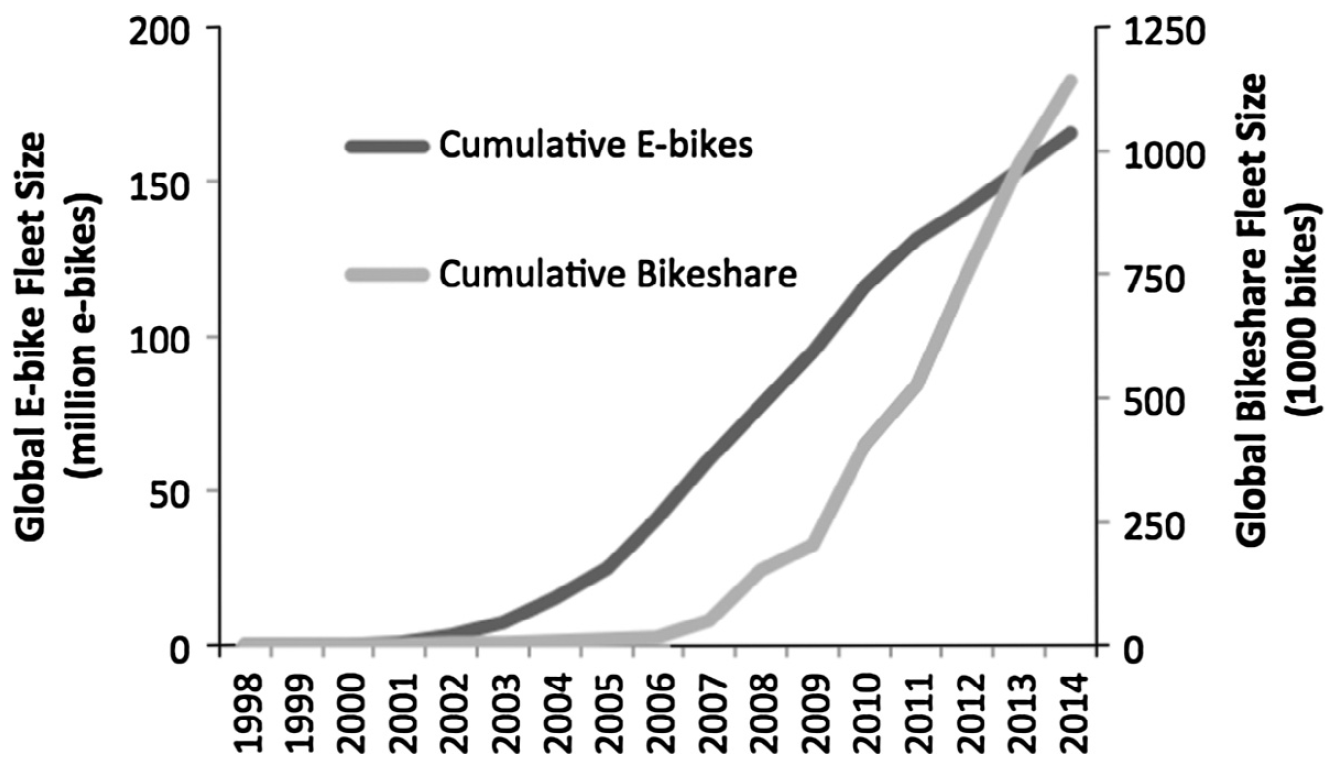
\includegraphics[width=0.6\linewidth]{image/bike_sharing} \caption{Growth in personal e-bike and public bikeshare systems (Campbell et al., 2016)}\label{fig:unnamed-chunk-56}
\end{figure}

Private BSS operators from China (\emph{Mobike, Ofo}) and Shanghai (\emph{oBike}) are currently introducing large fleets of station-less rental bikes in cities worldwide. The roll-out, especially in European cities, has encountered problems as city governments have not been able to coordinate the introduction (Zademach and Musch, 2018). Many bikes have been found abandoned around the cities. In addition, there are fears in some cases that the private companies introduced the BSS with the sole reason of tapping into private user data (Schöffel et al., 2017).
Furthermore, the company Montreal introduced ``BIXI'', fixed, portable, solar-powered and modular stations. They are self-contained and the stations can be placed, moved and relocated to desired locations within 20 minutes. ``Mega'' docking stations are available for special events (Midgley, 2011).
The number of BSSs has grown to over 800 units worldwide (Fishman, 2016). The public-private partnership model has been the most widespread, and the implementation of BSSs has been possible in cities with limited public funds (Zademach and Musch, 2018).
In Austria, there are multiple companies currently offering bicycle or e-bicycle sharing services. Former Citybike changed its service and name in April 2022 to WienMobil (powered by Nextbike). In the past, Asian providers of free floating rental bikes in Vienna (e.g.~ofo and oBike) ended their service due to non-compliance to new regulations (StVO Austria, 2018) requiring companies to pick up objectionable bikes on weekdays within four hours and at night/on weekends within twelve hours after notification (fines of up to 700, with a limit of 1500 euros), announced in August 2018 (Rachbauer, 2018b). Bikes now have to be registered and given a number in order to not exceed the upper limit of provided bikes per company (Blum, 2018) and meet certain criteria requested by the government (e.g.~having a headquarter and a service hotline).
Across Austria the situation with rental bikes differs a little in each federal state. Nevertheless, shared bikes are nowadays mostly powered by Nextbike (e.g.~Linz, Innsbruck, Lower Austria, Vienna) while Salzburg is still operating Citybike Salzburg which is linked to federal funding (Affenzeller, 2020, Citybike Salzburg, n.d. a). In Graz, there is no bicycle rental system, instead, stores and hotels offer rentals (Rachbauer, 2016). Moreover, \href{https://eddibike.com/?gclid=CjwKCAjw7vuUBhBUEiwAEdu2pBMaVQHIvD8XcgOxefvhXJPR20QXUyedzoNi4GoYQVeehfWpzkTLTBoCVR0QAvD_BwE}{EDDI Bike}, currently operating in Vienna and Graz, offers a bike where you can keep you bike for the cheapest rate of 24,99 per month. \href{https://en.ibike-box.com/mieten?gclid=CjwKCAjw7vuUBhBUEiwAEdu2pMBZKJQa9SmqgwCy7pGioNsPIcS-x6kaesuWFT3VliCCNT4rLgKlwhoCSSwQAvD_BwE}{Bike Box} is another service operating around Austria offering rental bikes from different providers in different areas, combined on their platform for easier access.

\hypertarget{relevant-initiatives-in-austria-57}{%
\subsection*{Relevant initiatives in Austria}\label{relevant-initiatives-in-austria-57}}
\addcontentsline{toc}{subsection}{Relevant initiatives in Austria}

\begin{itemize}
\tightlist
\item
  \href{https://firmenradl.at/cms/}{firmenradl.at}
\item
  \href{http://www.citybikesalzburg.at/}{citybikesalzburg}
\item
  \href{https://www.tips.at/nachrichten/linz/land-leute/523512-linzer-radverleih-startet-im-fruehjahr-an-40-standorten}{tpis.at}
\item
  \href{https://www.nextbike.at/en/}{Nextbike Austria}
\end{itemize}

\hypertarget{impacts-with-respect-to-sustainable-development-goals-sdgs-57}{%
\subsection*{Impacts with respect to Sustainable Development Goals (SDGs)}\label{impacts-with-respect-to-sustainable-development-goals-sdgs-57}}
\addcontentsline{toc}{subsection}{Impacts with respect to Sustainable Development Goals (SDGs)}

\begin{longtable}[]{@{}
  >{\centering\arraybackslash}p{(\columnwidth - 8\tabcolsep) * \real{0.2029}}
  >{\centering\arraybackslash}p{(\columnwidth - 8\tabcolsep) * \real{0.1884}}
  >{\centering\arraybackslash}p{(\columnwidth - 8\tabcolsep) * \real{0.2029}}
  >{\centering\arraybackslash}p{(\columnwidth - 8\tabcolsep) * \real{0.2029}}
  >{\centering\arraybackslash}p{(\columnwidth - 8\tabcolsep) * \real{0.2029}}@{}}
\toprule()
\begin{minipage}[b]{\linewidth}\centering
Impact level
\end{minipage} & \begin{minipage}[b]{\linewidth}\centering
Indicator
\end{minipage} & \begin{minipage}[b]{\linewidth}\centering
Impact direction
\end{minipage} & \begin{minipage}[b]{\linewidth}\centering
Goal description and number
\end{minipage} & \begin{minipage}[b]{\linewidth}\centering
Source
\end{minipage} \\
\midrule()
\endhead
Individual & Increased physical activity and improved health & \textbf{+} & Health \& wellbeing (\emph{3}) & Andersen et al., 2009 \\
Individual & Often first 30-60 minutes free of charge & \textbf{+} & Equality (\emph{5,10}) & Citybike Salzburg, n.d. b; Citybike Wien, n.d.; Nextbike Niederoesterreich, n.d. \\
Individual & Continuous advancement in bike features & \textbf{+} & Innovation \& Infrastructure (\emph{9}) & Zademach \& Musch, 2018 \\
Systemic & Wider access to this cheap or free mobility service & \textbf{+} & Equality (\emph{5,10}) & El Arbi \& Stephane, 2020 \\
Systemic & Air pollution, noise pollution and congestion reduced & \textbf{+} & Environmental sustainability (\emph{7,12,13,15}) & El Arbi \& Stephane, 2020 \\
Systemic & Investment in bike sharing infrastructure & \textbf{+} & Innovation \& Infrastructure (\emph{9}) & der Grazer, 2019; Hillebrand, 2019; Affenzeller, 2020; Tech \& Nature, 2020 \\
Systemic & 48\% of all systems are operated as public-private partnerships & \textbf{+} & Partnership \& collaborations (\emph{17}) & Midgley, 2011 \\
\bottomrule()
\end{longtable}

\hypertarget{technology-and-societal-readiness-level-57}{%
\subsection*{Technology and societal readiness level}\label{technology-and-societal-readiness-level-57}}
\addcontentsline{toc}{subsection}{Technology and societal readiness level}

\begin{longtable}[]{@{}cc@{}}
\toprule()
TRL & SRL \\
\midrule()
\endhead
7-9 & 5-7 \\
\bottomrule()
\end{longtable}

\hypertarget{open-questions-55}{%
\subsection*{Open questions}\label{open-questions-55}}
\addcontentsline{toc}{subsection}{Open questions}

\begin{enumerate}
\def\labelenumi{\arabic{enumi}.}
\tightlist
\item
  What measures can be implemented to tackle the vandalism of the bikes?
\item
  Which bike system (docked vs.~free-floating) is more sustainable in the long-term?
\end{enumerate}

\hypertarget{further-links-47}{%
\subsection*{Further links}\label{further-links-47}}
\addcontentsline{toc}{subsection}{Further links}

\begin{itemize}
\tightlist
\item
  \href{http://en.cyclocity.com/}{cyclocity.com}
\end{itemize}

\hypertarget{references-57}{%
\subsection*{References}\label{references-57}}
\addcontentsline{toc}{subsection}{References}

\begin{itemize}
\tightlist
\item
  Affenzeller, J. (2020, December 17). Linzer Radverleih startet im Frühjahr an 40 Standorten. \url{https://www.tips.at/nachrichten/linz/land-leute/523512-linzer-radverleih-startet-im-fruehjahr-an-40-standorten}
\item
  Andersen, L. B., Lawlor, D. A., Cooper, A. R., Froberg, K., and Anderssen, S. A. (2009). Physical fitness in relation to transport to school in adolescents: the Danish youth and sports study. Scandinavian Journal of Medicine \& Science in Sports, 19(3):406-411.
\item
  Campbell, A. A., Cherry, C. R., Ryerson, M. S., \& Yang, X. (2016). Factors influencing the choice of shared bicycles and shared electric bikes in Beijing. Transportation Research Part C: Emerging Technologies, 67, 399--414. \url{https://doi.org/10.1016/j.trc.2016.03.004}
\item
  Cheng, L., Yang, J., Chen, X., Cao, M., Zhou, H., \& Sun, Y. (2020). How could the station-based bike sharing system and the free-floating bike sharing system be coordinated? Journal of Transport Geography, 89(March 2019), 102896. \url{https://doi.org/10.1016/j.jtrangeo.2020.102896}
\item
  Cheng, X., \& Gao, Y. (2018). The Optimal Monthly Strategy Pricing of Free-Floating Bike Sharing Platform. Modern Economy, 09(02), 318--338. \url{https://doi.org/10.4236/me.2018.92021}
\item
  Citybike Salzburg. (n.d.-a). Citybike Salzburg. Available at: \url{http://www.citybikesalzburg.at/hanuschplatz.php} {[}Accessed: 12 January 2021{]}
\item
  Citybike Salzburg. (n.d.-b). Citybike Salzburg - Tarife. Available at: \url{http://www.citybikesalzburg.at/tarife.php} {[}Accessed: 18 January 2021{]}
\item
  Citybike Wien. (n.d.). Tarife - Citybike Wien. Available at: \url{https://www.citybikewien.at/de/tarife} {[}Accessed: 18 January 2021{]}
\item
  Citybike Wien. (2019). 10 Millionen Fahrten bei Citybike Wien! Available at: \url{https://www.citybikewien.at/de/news/595-neuer-meilenstein-bei-citybike-wien-erreicht} {[}Accessed: 17 January 2021{]}
\item
  DeMaio, P. (2009). Bike-sharing: History, Impacts, Models of Provision, and Future. Journal of Public Transportation, 12(4), 41--56. \url{https://doi.org/10.5038/2375-0901.12.4.3}
\item
  der Grazer. (2019, October 21). 100 Millionen Euro für Fahrrad-Offensive im Großraum Graz -- Der Grazer. Available at: \url{https://grazer.at/de/uHAnk5t2/100-millionen-euro-fuer-fahrrad-offensive-im-graz/} {[}Accessed: 17 January 2021{]}
\item
  Eillie, A. (2016). Oxford Test Drives Peer-to-Peer Bike Sharing. \url{https://www.bloomberg.com/news/articles/2016-09-13/cycle-land-is-a-new-peer-to-peer-bike-sharing-platform}
\item
  El Arbi, A. A., \& Stephane, C. K. T. (2020). Intelligent Management of Bike Sharing in Smart Cities using Machine Learning and Internet of Things. Sustainable Cities and Society, 135907. \url{https://doi.org/10.1016/j.scs.2020.102702}
\item
  Fishman, E. (2016). Bikeshare: A Review of Recent Literature. Transport Reviews, 36(1), 92--113. \url{https://doi.org/10.1080/01441647.2015.1033036}
\item
  Fishman, E., Washington, S., Haworth, N., \& Mazzei, A. (2014). Barriers to bikesharing: An analysis from Melbourne and Brisbane. Journal of Transport Geography, 41, 325--337. \url{https://doi.org/10.1016/j.jtrangeo.2014.08.005}
\item
  Gu, T., Kim, I., \& Currie, G. (2019). To be or not to be dockless: Empirical analysis of dockless bikeshare development in China. Transportation Research Part A: Policy and Practice, 119, 122--147. \url{https://doi.org/10.1016/j.tra.2018.11.007}
\item
  Hillebrand, T. (2019). Mietradsystem `Stadtrad Innsbruck' - VCÖ Vorbildhafte Mobilitätsprojekte. Available at: \url{https://mobilitaetsprojekte.vcoe.at/mietradsystem-stadtrad-innsbruck-2019} {[}Accessed: 17 January 2021{]}
\item
  Li, H., Zhang, Y., Ding, H., \& Ren, G. (2019). Effects of dockless bike-sharing systems on the usage of the London Cycle Hire. Transportation Research Part A: Policy and Practice, 130, 398--411. \url{https://doi.org/10.1016/j.tra.2019.09.050}
\item
  Ma, X., Ji, Y., Yuan, Y., Van Oort, N., Jin, Y., \& Hoogendoorn, S. (2020). A comparison in travel patterns and determinants of user demand between docked and dockless bike-sharing systems using multi-sourced data. Transportation Research Part A: Policy and Practice, 139(June), 148--173. \url{https://doi.org/10.1016/j.tra.2020.06.022}
\item
  Midgley, P. (2011). Bicycle-Sharing Schemes: Enhancing Sustainable Mobility in Urban Areas. Commission on Sustainable Development, Nine teent(8), 24. \url{http://www.un.org/esa/dsd/resources/res_pdfs/csd-19/Background-Paper8-P.Midgley-Bicycle.pdf}
\item
  Nextbike Niederösterreich. (n.d.). Nextbike Niederösterreich - Tarife. Available at: \url{https://www.nextbike.at/de/niederoesterreich/preise/} {[}Accessed: 18 January 2021{]}
\item
  Rachbauer, S. (2016, July). Bikesharing in Österreich: Leihräder auf der Überholspur \textbar{} kurier.at. \url{https://kurier.at/chronik/oesterreich/bikesharing-in-oesterreich-leihraeder-auf-der-ueberholspur/400067369}
\item
  Rachbauer, S. (2018a). Bikesharing in Österreich: Leihräder auf der Überholspur. \url{https://kurier.at/chronik/oesterreich/bikesharing-in-oesterreich-leihraeder-auf-der-ueberholspur/400067369}
\item
  Rachbauer, S. (2018b). Leihräder: Wiener wollen es aufgeräumt. \url{https://kurier.at/chronik/wien/leihraeder-wiener-wollen-es-aufgeraeumt/400067357}
\item
  Rachbauer, S. (2018c, March). Wien führt strenge Regeln für stationslose Leihräder ein. \url{https://kurier.at/chronik/wien/wien-fuehrt-strenge-regeln-fuer-stationslose-leihraeder-ein/312.944.617}
\item
  Rachbauer, S. (2018d, July 17). Leihräder: Wiener wollen es aufgeräumt. \url{https://kurier.at/chronik/wien/leihraeder-wiener-wollen-es-aufgeraeumt/400067357}
\item
  Schöffel, R., Zierer, M., \& Kühne, S. (2017). Nutzerdaten offen im Netz: BR deckt Datenleck beim Fahrradverleiher Obike auf. \url{https://www.br.de/nachricht/datenleck-obike-100.html}
\item
  Sun, S., \& Ertz, M. (2021). Contribution of bike-sharing to urban resource conservation: The case of free-floating bike-sharing. Journal of Cleaner Production, 280, 124416. \url{https://doi.org/10.1016/j.jclepro.2020.124416}
\item
  Tech \& Nature. (2020, April 28). Niederösterreich modernisiert Sharing-Bike-Flotte `nextbike' - Tech \& Nature. \url{https://www.techandnature.com/niederosterreich-modernisiert-sharing-bike-flotte-nextbike/}
\item
  Zademach, H. M., \& Musch, A. K. (2018). Bicycle-sharing systems in an alternative/diverse economy perspective: a sympathetic critique. Local Environment, 23(7), 734--746. \url{https://doi.org/10.1080/13549839.2018.1434494}
\item
  Zhang, Y., Lin, D., \& Mi, Z. (2019). Electric fence planning for dockless bike-sharing services. Journal of Cleaner Production, 206, 383--393. \url{https://doi.org/10.1016/j.jclepro.2018.09.215}
\end{itemize}

\hypertarget{scooters}{%
\section{E-scooters sharing}\label{scooters}}

\textbf{Updated: 8th June 2022}

\hypertarget{synonyms-52}{%
\subsection*{Synonyms}\label{synonyms-52}}
\addcontentsline{toc}{subsection}{Synonyms}

\emph{electric scooter}

\hypertarget{definition-58}{%
\subsection*{Definition}\label{definition-58}}
\addcontentsline{toc}{subsection}{Definition}

E-kick scooters are electrically powered scooters that, after an initial push-off with a push lever, accelerate and then move at a speed similar to bicycles. They are one of micro-mobility solutions which is growing trend in urban mobility. It encompasses all human-powered micro-vehicles, such as bicycles and scooters, but also new micro-vehicles such as e-scooters, e-bikes and some other small, electrically powered vehicles (Oeschger, Carroll and Caulfield, 2020). Most of the modern vehicles of this type are available for both shared and private use and are gaining wide acceptance.
E-scooters have promised a solution to the last mile problem since their introduction in 2017 (Siegfried et al, 2021). They are seen as alternatives to cars and provide potential for reducing traffic congestion, noise and pollution. Initial results suggest that e-scooters are mainly used for distances between 1 and 6 km. Empirical evidence shows that e-scooters can substitute walking rather than driving for these short distances (James et al., 2019; Portland Bureau of Transportation, 2019). In addition to the potential positive environmental impact of e-scooters on the transportation system, some safety concerns have been raised. Most e-scooter users who had an accident have ridden without a helmet (Liew et al, 2020). In general, e-scooters are almost exclusively issued without protective equipment (Allem and Majmundar, 2019). The safety issues do not only affect the riders themselves, but also have an impact on other road users, especially pedestrians (Sikka et al., 2019). It has even been criticised that technology follows the idea of ``sell first, safety later'' (Choron and Sakran, 2019).

\hypertarget{key-stakeholders-58}{%
\subsection*{Key stakeholders}\label{key-stakeholders-58}}
\addcontentsline{toc}{subsection}{Key stakeholders}

\begin{itemize}
\tightlist
\item
  \textbf{Affected}: Mobile citizens, pedestrians, insurers
\item
  \textbf{Responsible}: National governments, city government, private Companies
\end{itemize}

\hypertarget{current-state-of-art-in-research-58}{%
\subsection*{Current state of art in research}\label{current-state-of-art-in-research-58}}
\addcontentsline{toc}{subsection}{Current state of art in research}

Since e-scooters are already well-established technology, most research focuses on safety and accidents, user behaviour and potential environmental impact of uptake of this micro-mobility option. Some studies advocate e-scooters as an environmentally friendly solution for crowded cities, others report contradictory results and point to safety issues.
Moreover, research also explores whether the presence of e-scooters reduces bicycle thefts (Gössling, 2020). In Gothenburg, Sweden, the police reported that the number of bicycle thefts halved after the introduction of e-scooters and rental bikes (Sydsvenskan, 2019). For a safe integration of micro mobility into the transport system, the study from Dozza et al.~(2022) found, that e-scooters may be more maneuverable and comfortable than bikes but need longer braking distances. It is suggested that data from e-scooters is collected to facilitate policy making and education in the future. Additionally, there is still an ongoing discourse about e-scooters and the competition to bicycles and the public transport and a potential contribution to the last mile problem (Nawaro, 2021).

\hypertarget{current-state-of-art-in-practice-58}{%
\subsection*{Current state of art in practice}\label{current-state-of-art-in-practice-58}}
\addcontentsline{toc}{subsection}{Current state of art in practice}

E-scooter providers such as \emph{Lime} and \emph{Bird}, which launched operations in California in 2017, can now be found in over 100 cities worldwide and have since recorded millions of rides. E-scooter provider \emph{VOI} has experienced similar growth in Europe and entered the market in 10 countries in just one year after launching in Sweden and has recorded over 16 million rides (Oeschger et al., 2020). The results of a survey indicate that e-scooters are primarily seen as entertainment and not as a means of transport (Siegfried et al., 2021).
Maximum speed limits are an important issue and internationally there are different approaches. Los Angeles and Dallas, for example, have no speed limit, as far as can be deduced from the news; while the limit in Vienna is 25 km/h (Schwarz, 2019). Paris is discussing reducing the speed limit to 20 km/h on cycle paths and 8 km/h in parks and pedestrian areas (Négroni, 2019). One problem with the maximum speeds is that some of the e-scooter models can go much faster than 25 km/h (Le Figaro, 2018). To counteract the negative consequences of the introduction of e-scooters, cities have evaluated and implemented various rules and guidelines. Media analysis suggests that the city councils should introduce the following rules as a minimal requirement: speed limits, restrictions on the exclusive use of bicycle infrastructure and a designation of parking spaces for rental and return. Behavioural campaigns and fines, are needed to limit negative consequences of e-scooter use (Gössling, 2020). Petzoldt et al.~(2021) analysed that a lack of awareness, together with a lack of agreement causes the most violations of existing rules.
In Vienna, only very few e-scooters are used on bicycle paths (between 4.9\% and 7.1\% compared to other bicycle path users). Given the modal split of Vienna (7\% cycling), it can be concluded that e-scooters do not yet have a significant role in Vienna's transport system (Laa and Leth, 2020). In the last year (2021) there was no significant study implicating that e-scooters' share in model split has increased. Nevertheless e-scooters and their sharing capacity becomes more prominent with each day in Austria. Current regulations in Vienna (Austria) can be found \href{https://www.oesterreich.gv.at/themen/freizeit_und_strassenverkehr/Elektro-Scooter,-Quads-und-Co/Seite.610110.html}{here}, while operating companies are currently Lime, Bird, Tier, Link and KiwiRide. An overview over pricing and parking policies in Vienna can be found \href{https://autorevue.at/ratgeber/e-scooter-wien-vergleich}{here}.

\hypertarget{relevant-initiatives-in-austria-58}{%
\subsection*{Relevant initiatives in Austria}\label{relevant-initiatives-in-austria-58}}
\addcontentsline{toc}{subsection}{Relevant initiatives in Austria}

\begin{itemize}
\tightlist
\item
  \href{https://autorevue.at/ratgeber/e-scooter-wien-vergleich}{autorevue.at}
\item
  \href{https://www.stadt-wien.at/wien/news/e-scooter-sharing-system-in-wien.html}{stadt-wien.at}
\item
  \href{https://www.wien.gv.at/english/transportation-urbanplanning/scooter.html}{wien.gv.at}
\item
  \href{https://www.oeamtc.at/thema/fahrrad/e-kleintretroller-e-scooter-in-oesterreich-31721872}{oeamtc.at}
\item
  \href{https://www.oesterreich.gv.at/themen/freizeit_und_strassenverkehr/Elektro-Scooter,-Quads-und-Co/Seite.610110.html}{oesterreich.gv.at}
\end{itemize}

\hypertarget{impacts-with-respect-to-sustainable-development-goals-sdgs-58}{%
\subsection*{Impacts with respect to Sustainable Development Goals (SDGs)}\label{impacts-with-respect-to-sustainable-development-goals-sdgs-58}}
\addcontentsline{toc}{subsection}{Impacts with respect to Sustainable Development Goals (SDGs)}

\begin{longtable}[]{@{}
  >{\centering\arraybackslash}p{(\columnwidth - 8\tabcolsep) * \real{0.2029}}
  >{\centering\arraybackslash}p{(\columnwidth - 8\tabcolsep) * \real{0.1884}}
  >{\centering\arraybackslash}p{(\columnwidth - 8\tabcolsep) * \real{0.2029}}
  >{\centering\arraybackslash}p{(\columnwidth - 8\tabcolsep) * \real{0.2029}}
  >{\centering\arraybackslash}p{(\columnwidth - 8\tabcolsep) * \real{0.2029}}@{}}
\toprule()
\begin{minipage}[b]{\linewidth}\centering
Impact level
\end{minipage} & \begin{minipage}[b]{\linewidth}\centering
Indicator
\end{minipage} & \begin{minipage}[b]{\linewidth}\centering
Impact direction
\end{minipage} & \begin{minipage}[b]{\linewidth}\centering
Goal description and number
\end{minipage} & \begin{minipage}[b]{\linewidth}\centering
Source
\end{minipage} \\
\midrule()
\endhead
Individual & E-scooter trips replace mainly walking trips & \textbf{-} & Health \& Wellbeing (\emph{3}) & Laa \& Leth, 2020; Nawaro 2021 \\
Individual & More expensive compared to public transport & \textbf{-} & Sustainable economic development (\emph{8,11}) & Widholm, 2021; Wiener Linien, 2021 \\
Individual & Increase in participants on existing cycling infrastructure & \textbf{\textasciitilde{}} & Innovation \& Infrastructure (\emph{9}) & Laa \& Leth, 2020; Nawaro 2021 \\
Systemic & Highest user share among young males & \textbf{-} & Equality (\emph{5,10}) & Laa \& Leth, 2020; Reck, 2021 \\
Systemic & E-scooter trips replace more sustainable transport modes & \textbf{-} & Environmental sustainability (\emph{7,12,13,15}) & Laa \& Leth, 2020; Nawaro 2021 \\
Systemic & Growth in micromobility sector & \textbf{+} & Sustainable economic development (\emph{8,11}) & Goessling, 2020 \\
\bottomrule()
\end{longtable}

\hypertarget{technology-and-societal-readiness-level-58}{%
\subsection*{Technology and societal readiness level}\label{technology-and-societal-readiness-level-58}}
\addcontentsline{toc}{subsection}{Technology and societal readiness level}

\begin{longtable}[]{@{}cc@{}}
\toprule()
TRL & SRL \\
\midrule()
\endhead
7-9 & 7-9 \\
\bottomrule()
\end{longtable}

\hypertarget{open-questions-56}{%
\subsection*{Open questions}\label{open-questions-56}}
\addcontentsline{toc}{subsection}{Open questions}

\begin{enumerate}
\def\labelenumi{\arabic{enumi}.}
\tightlist
\item
  Will an increasing presence of e-scooters on the bicycle infrastructure or in pedestrian zones require separate solution in urban road infrastructure?
\end{enumerate}

\hypertarget{references-58}{%
\subsection*{References}\label{references-58}}
\addcontentsline{toc}{subsection}{References}

\begin{itemize}
\tightlist
\item
  Allem, J. P., \& Majmundar, A. (2019). Are electric scooters promoted on social media with safety in mind? A case study on Bird's Instagram. In Preventive Medicine Reports (Vol. 13, pp.~62--63). Elsevier Inc.~\url{https://doi.org/10.1016/j.pmedr.2018.11.013}
\item
  Choron, R. L., \& Sakran, J. V. (2019). The Integration of Electric Scooters: Useful Technology or Public Health Problem? American Journal of Public Health, 109(4), 555--556. \url{https://doi.org/10.2105/AJPH.2019.304955}
\item
  Dozza, M., Violin, A., Rasch, A. (2022). A data-driven framework for the safe integration of micro-mobility into the transport system: Comparing bicycles and e-scooters in field trials. Journal of Safety Research. 81, 67-77. \url{https://doi.org/10.1016/j.jsr.2022.01.007}
\item
  Gössling, S. (2020). Integrating e-scooters in urban transportation: Problems, policies, and the prospect of system change. Transportation Research Part D: Transport and Environment, 79(January), 102230. \url{https://doi.org/10.1016/j.trd.2020.102230}
\item
  James, O., Swiderski, J., Hicks, J., Teoman, D., \& Buehler, R. (2019). Pedestrians and E-Scooters: An Initial Look at E-Scooter Parking and Perceptions by Riders and Non-Riders. Sustainability, 11(20), 5591. \url{https://doi.org/10.3390/su11205591}
\item
  Laa, B., \& Leth, U. (2020). Survey of E-scooter users in Vienna: Who they are and how they ride. Journal of Transport Geography, 89(October), 102874. \url{https://doi.org/10.1016/j.jtrangeo.2020.102874}
\item
  Le Figaro. (2018, September 9). Trottinettes: la mairie de Paris veut une réglementation nationale. \url{https://www.lefigaro.fr/flash-eco/2018/09/09/97002-20180909FILWWW00064-trottinettes-la-mairie-de-paris-veut-une-reglementation-nationale.php}
\item
  Liew, Y. K., Wee, C. P. J., \& Pek, J. H. (2020). New peril on our roads: A retrospective study of electric scooter-related injuries. Singapore Medical Journal, 61(2), 92--95. \url{https://doi.org/10.11622/smedj.2019083}
\item
  Nawaro, L. (2021). E-scooters: competition with sahred bicycles and relationship to public transport. International Journal of Urban Sustainable Development, 13 (3). \url{https://doi.org/10.1080/19463138.2021.1981336}
\item
  Négroni, A. (2019, June 6). Paris: Hidalgo prend des mesures contre les trottinettes électriques. \url{https://www.lefigaro.fr/actualite-france/trottinettes-paris-prend-des-mesures-20190606}
\item
  OECD/ITF. (2020). Safe Micromobility. 98. \url{https://www.itf-oecd.org/safe-micromobility}
\item
  Oeschger, G., Carroll, P., \& Caulfield, B. (2020). Micromobility and public transport integration: The current state of knowledge. Transportation Research Part D: Transport and Environment, 89, 102628. \url{https://doi.org/10.1016/j.trd.2020.102628}
\item
  Petzholdt, T., Ringhand, M., Anke, J., Schekatz, N. (2021). Do German (non)Users of e-scooters know the rule (and do they agree with them?). HCII 2021: HCI in Mobility, Transport and Automative Systems. 425-435
\item
  Portland Bureau of Transportation. (2019). 2018 E-Scooter Findings Report. \url{https://www.portlandoregon.gov/transportation/article/709719\%0Ahttps://trid.trb.org/view/1607260}
\item
  Reck, D. J., Ashausen, K. W. (2021). Who uses shared micro-mobility services? Empirical evidence from Zurich, Switzerland. Transportation Research Part D: Transport and Environment, 94 (102803), 1-11. \url{https://doi.org/10.1016/j.trd.2021.102803}
\item
  Schwarz, R. (2019, July 27). E-Bikes und E-Scooter sind viel zu schnell! - Ideen-Blog - derStandard.at › Diskurs. \url{https://www.derstandard.at/story/2000106514149/e-bikes-und-e-scooter-sind-viel-zu-schnell}
\item
  Siegfried, C., Martin, B., \& Reichenberger, Y. (2021). Consumer acceptance of shared e-scooters for urban and short-distance mobility. Transportation Research Part D, 91(January), 102680. \url{https://doi.org/10.1016/j.trd.2020.102680}
\item
  Sikka, N., Vila, C., Stratton, M., Ghassemi, M., \& Pourmand, A. (2019). Sharing the sidewalk: A case of E-scooter related pedestrian injury. American Journal of Emergency Medicine, 37(9), 1807.e5-1807.e7. \url{https://doi.org/10.1016/j.ajem.2019.06.017}
\item
  Sydsvenskan. (2019, August 30). Elsparkcyklarna minskar cykelstölderna - Sydsvenskan. Available at: \url{https://www.sydsvenskan.se/2019-08-30/elsparkcyklarna-minskar-cykelstolderna} {[}Accessed: 20 January 2021{]}
\item
  Widholm, K. (n.d.). E-Scooter Sharing-System: Roller von Lime, Tier, Bird und Co.~Available at: \url{https://www.stadt-wien.at/wien/news/e-scooter-sharing-system-in-wien.html} {[}Accessed: 20 January 2021{]}
\item
  Wiener Linien. (n.d.). Übersicht Tickets \textbar{} Tickets \textbar{} Fahrgastinfo \textbar{} Wiener Linien. Available at: \url{https://www.wienerlinien.at/eportal3/ep/channelView.do/pageTypeId/66526/channelId/-46648} {[}Accessed: 20 January 2021{]}
\item
  Zagorskas, J., \& Burinskiene, M. (2020). Challenges caused by increased use of E-powered personal mobility vehicles in European cities. Sustainability (Switzerland), 12(1), 273. \url{https://doi.org/10.3390/su12010273}
\end{itemize}

\hypertarget{ride_hailing}{%
\section{Ride hailing and ride sharing}\label{ride_hailing}}

\textbf{Updated: 11th July 2022}

\hypertarget{synonyms-53}{%
\subsection*{Synonyms}\label{synonyms-53}}
\addcontentsline{toc}{subsection}{Synonyms}

\begin{itemize}
\tightlist
\item
  Ride hailing: \emph{Ridesourcing, app-based ride services, ride-booking, on-demand ride services, Transportation Network Companies (TNCs), mobility service providers (MSPs)}
\item
  Ride sharing: \emph{car-pooling}
\end{itemize}

\hypertarget{definition-59}{%
\subsection*{Definition}\label{definition-59}}
\addcontentsline{toc}{subsection}{Definition}

Ride sharing and ride hailing both emerged from the ``shared economy'' or ``collaborative economy'', which aims to share underutilized resources to increase efficiency, protect the environment and promote economic growth (Tirachini, 2019).

Ride hailing (RH) enables booking a journey via an online platform -- usually an app. The platforms match travellers who want to book a specific ride with a personal driver who is willing to take that ride in their private car, based on their location. Ride-hailing platforms mostly eliminate the exchange of cash and apply basic economic principles to match supply and demand through dynamic price adjustments. However, this original model is not allowed in all countries. In Austria, for example, it is not allowed to offer ride hailing with one's private car, only with rental cars. Since 2021, drivers are also required to have a Viennese taxi driver's license (Uber Technologies Inc., n.d.).

Ride sharing, by contrast, describes the process in which a rider shares a vehicle with multiple other riders, who want to go in the same direction. Some Transportation Network Companies who offer ride hailing are also offering ride sharing services, like \emph{UberPool} or \emph{Lyft Shared} which are usually cheaper and also more environmentally friendly due to the higher occupancy rate (Herzog, 2018). Dynamic ride sharing systems use algorithms to match riders, who want to go in a similar direction and form a shared ride (Lokhandwala \& Cai, 2018).

\hypertarget{key-stakeholders-59}{%
\subsection*{Key stakeholders}\label{key-stakeholders-59}}
\addcontentsline{toc}{subsection}{Key stakeholders}

\begin{itemize}
\tightlist
\item
  \textbf{Affected}: Mobile Citizen, Taxi Drivers
\item
  \textbf{Responsible}: National Governments, City government, Private Companies, Transportation Network Companies, Software providers
\end{itemize}

\hypertarget{current-state-of-art-in-research-59}{%
\subsection*{Current state of art in research}\label{current-state-of-art-in-research-59}}
\addcontentsline{toc}{subsection}{Current state of art in research}

Even though ride hailing emerged from the sharing economy, it is controversial whether it has ultimately had a positive effect on the environment (Herzog, 2018).

Jan et al.~(2018) argue that ride hailing has a positive impact on economic efficiency. As it both complements and competes with public transport, its impact on congestion near city centres is still unclear. In terms of equity, ride hailing reinforces the problem of the digital gap and raises concerns about discrimination, privacy and security. It is also controversial whether prosumers (producers/consumers) are exploited by sharing economy platforms, whether ride hailing drivers are adequately compensated and how the rights of on-demand workers can be better protected. Even though ride hailing likes to present itself with a green image, the actual environmental impacts have not yet been thoroughly investigated. Further, Jin et al.~(2018) pointed out the danger of conceptual confusion in ride hailing research. Based on evidences reported in the literature, they argue, that it is unlikely, that people stop owning cars due to ride hailing. A recent study by Cats et al.~(2021) suggests that the dichotomy of ``competing with or complementing'' is false, even if the vast majority of ride hailing trips have a viable public transport alternative, between 20-40\% of them have not. Ride hailing patterns do not only depend on availability but also on accessibility, difference in travel times between public transport and ride hailing and must be assessed separately for each case. Yang et al.~(2022), in turn, simulated the suspension of ride hailing trips and found a decrease of 50\% vehicle emissions related to ride sourcing with a mode shift to public transport (50\%), taxi (27\%), active mode (11\%) and private car trips (7\%).

Regarding ride sharing, Alisoltani et al.~(2012) argue, that it can reduce traffic congestion, but only if the trip density is high, which is usually the case in large-scale networks. In smaller cities, with a small- or medium-scale network, the trip density is not high enough. Importantly, trip density is defined as the total number of trips ends (origins and destinations) within 24 h within a given area (Miller \& Soberman, 2003).

Lokhandwala \& Cai (2018) compared in a case study in New York City shared autonomous vehicles (SAVs) to traditional taxis and found out that SAVs have the potential to reduce the fleet size in NYC by more than 50\% and reduce daily greenhouse gas emissions by up to 866 MT of CO\textsubscript{2} eq.

The study by Martin et al.~(2021) provides a recent review of studies on ridesharing optimization. They compare different analytical approaches in this research area and discuss the emerging concept of ``agile'' algorithms that could help to cope with the demands of large-scale and dynamic optimization problems for ridesharing.

The NGO Mothers Against Drunk Driving (MADD) and Uber -- one of the most known ride hailing platforms -- published a report in 2015, in which they argue, based on studies in California, that the presence of uber services in a city can lower the amount of drunk driving crashes involving younger populations. Based on a study of Seattle's data, they argue that Uber's entry into the Seattle market was associated with a 10\% drop in drunk driving arrests.

\hypertarget{current-state-of-art-in-practice-59}{%
\subsection*{Current state of art in practice}\label{current-state-of-art-in-practice-59}}
\addcontentsline{toc}{subsection}{Current state of art in practice}

The two most known companies offering ride hailing in the US are \emph{Uber} and \emph{Lyft}. Uber, for instance, again offers various services, such as:

\begin{itemize}
\tightlist
\item
  UberX - affordable rides, door to door, all to yourself
\item
  UberPool - shared rides, door to door or with a short walk
\item
  UberGreen - sustainable rides in electric vehicles - or many more.
\end{itemize}

Due to regulations and uprisings of local cab companies, Uber had to adapt its business model for European cities. Other ride hailing platforms operating in Western and Central Europe are \emph{Gett, Bolt, Hailo} or \emph{Taxilo}. They all have small differences and vary based on the drivers' commission fee to the particular platform (Khatri, 2020a).

Before the Covid-19 pandemic, the ride hailing marked had been growing fast. Like other industries, the ride hailing market dropped in 2020 globally, due to the crisis and related measures, such as lockdowns, social distancing, etc. To survive, some of the bigger companies, like Uber e.g., started to foray into on-demand food delivery and parcel delivery. The industry is expected to recover depending on how quickly the general economy recovers from the crisis. Nevertheless, there will be differences in speed between countries, regions and social groups. Looking to the post-Covid era, ride hailing drivers will have to implement various safety measures, like e.g.~frequent sanitation, wearing masks, guarantee tracing, to win back the trust of customers. Mushahid Khatri (2021), a Chief Executive Officer of \href{https://www.yelowsoft.com/}{Yelowsoft} expects ``that ride-hailing companies will move towards transit authorities for providing on-demand shuttle \& bus services''. Secondly, he thinks that ride hailing companies should make sure they are part of MaaS (see section on \protect\hyperlink{maas}{MaaS}) and use Artificial Intelligence (AI) to improve their services (Khatri, 2020b).

The world's largest long-distance ride-sharing app, which has 90 million members, is \emph{BlaBlaCar}. Every quarter, 25 million global travellers use BlaBlaCar to organize their car trip and thus share the cost of travel (BlaBlaCar, 2021). Similar to other platforms based on the sharing economy, safety is ensured through a rating system where riders can rate other passengers and vice versa.

The Austrian platforms \emph{GREENDRIVE} and \emph{Carployee} both connect drivers who work for the same companies or institutions with the goal of saving company parking spaces through shared rides and protecting the environment at the same time (GREENDRIVE MOBILITY GMBH, 2020; Carployee, 2020).

\hypertarget{relevant-initiatives-in-austria-59}{%
\subsection*{Relevant initiatives in Austria}\label{relevant-initiatives-in-austria-59}}
\addcontentsline{toc}{subsection}{Relevant initiatives in Austria}

\begin{itemize}
\tightlist
\item
  \href{https://www.ots.at/presseaussendung/OTS_20210113_OTS0026/free-now-will-als-erste-mobilitaetsplattform-in-europa-bis-2030-null-emissionen-erreichen}{ots.at}
\item
  \href{https://www.umweltberatung.at/carsharing-mitfahrboersen}{umweltberatung.a}
\item
  \href{https://greendrive.at/premium/\#benefits}{greendrive.a}
\item
  \href{https://www.carployee.com/\#start-section}{carployee.com}
\item
  \href{https://ummadum.com/}{ummadum.com}
\item
  \href{https://www.carpoolworld.com/carpool_AUSTRIA_favorites.html}{CarpoolWorld}
\item
  \href{http://www.foahstmit.at}{Foahstmit.at}
\end{itemize}

\hypertarget{impacts-with-respect-to-sustainable-development-goals-sdgs-59}{%
\subsection*{Impacts with respect to Sustainable Development Goals (SDGs)}\label{impacts-with-respect-to-sustainable-development-goals-sdgs-59}}
\addcontentsline{toc}{subsection}{Impacts with respect to Sustainable Development Goals (SDGs)}

\begin{longtable}[]{@{}
  >{\centering\arraybackslash}p{(\columnwidth - 8\tabcolsep) * \real{0.2029}}
  >{\centering\arraybackslash}p{(\columnwidth - 8\tabcolsep) * \real{0.1884}}
  >{\centering\arraybackslash}p{(\columnwidth - 8\tabcolsep) * \real{0.2029}}
  >{\centering\arraybackslash}p{(\columnwidth - 8\tabcolsep) * \real{0.2029}}
  >{\centering\arraybackslash}p{(\columnwidth - 8\tabcolsep) * \real{0.2029}}@{}}
\toprule()
\begin{minipage}[b]{\linewidth}\centering
Impact level
\end{minipage} & \begin{minipage}[b]{\linewidth}\centering
Indicator
\end{minipage} & \begin{minipage}[b]{\linewidth}\centering
Impact direction
\end{minipage} & \begin{minipage}[b]{\linewidth}\centering
Goal description and number
\end{minipage} & \begin{minipage}[b]{\linewidth}\centering
Source
\end{minipage} \\
\midrule()
\endhead
Individual & Increased accessibility & \textbf{+} & Equality (\emph{5,10}) & Abdelwahab, 2020; Tirachini, 2019 \\
Systemic & Reduced accidents by drunk drivers & \textbf{+} & Health \& Wellbeing (\emph{3}) & Uber \& MADD, 2015 \\
Systemic & Decreased emissions per capita & \textbf{+} & Environmental sustainability (\emph{7,12,13,15}) & Tirachini, 2019 \\
Systemic & Increased motorized traffic and congestion; positive impact on economic efficiency & \textbf{\textasciitilde{}} & Sustainable economic development (\emph{8,11}) & Tirachini, 2019; Jin et al., 2018 \\
\bottomrule()
\end{longtable}

\hypertarget{technology-and-societal-readiness-level-59}{%
\subsection*{Technology and societal readiness level}\label{technology-and-societal-readiness-level-59}}
\addcontentsline{toc}{subsection}{Technology and societal readiness level}

\begin{longtable}[]{@{}cc@{}}
\toprule()
TRL & SRL \\
\midrule()
\endhead
7-9 & 6-9 \\
\bottomrule()
\end{longtable}

\hypertarget{open-questions-57}{%
\subsection*{Open questions}\label{open-questions-57}}
\addcontentsline{toc}{subsection}{Open questions}

\begin{enumerate}
\def\labelenumi{\arabic{enumi}.}
\tightlist
\item
  How to overcome the rising concerns over discrimination and data privacy and security?
\item
  Which impacts of ride-hailing on traffic congestion outweigh the others?
\item
  How can the environmental impacts of ride hailing be reliably and holistically analysed?
\item
  How can ride-hailing and ride-sharing discourage private car ownership?
\item
  Do ride-sharing and ride-hailing compete and/or complement each other?
\end{enumerate}

\hypertarget{further-links-48}{%
\subsection*{Further links}\label{further-links-48}}
\addcontentsline{toc}{subsection}{Further links}

\begin{itemize}
\tightlist
\item
  \href{https://www.ots.at/presseaussendung/OTS_20210113_OTS0026/free-now-will-als-erste-mobilitaetsplattform-in-europa-bis-2030-null-emissionen-erreichen}{ots.at}
\item
  \href{https://www.umweltberatung.at/carsharing-mitfahrboersen}{umweltberatung.at}
\item
  \href{https://greendrive.at/premium/\#benefits}{greendrive}
\item
  \href{https://www.carployee.com/\#start-section}{carployee}
\item
  \href{https://ummadum.com/}{ummadum.com}
\item
  \href{https://www.blablacar.de/}{blablacar}
\item
  \href{https://www.uber.com/at/de/}{uber}
\end{itemize}

\hypertarget{references-59}{%
\subsection*{References}\label{references-59}}
\addcontentsline{toc}{subsection}{References}

\begin{itemize}
\tightlist
\item
  Abdelwahab, B. (2020). Ridesharing and Social Inclusion: The Role of Ridesharing in Improving Job Access for Disadvantaged Populations (Doctoral dissertation).
\item
  Alisoltani, N., Leclercq, L., \& Zargayouna, M. (2021). Can dynamic ride-sharing reduce traffic congestion?. Transportation research part B: methodological, 145, 212-246.
\item
  BlaBlaCar. (2021). Über uns - BlaBlaCar. \url{https://blog.blablacar.de/about-us}
\item
  Carployee. (2020). Carployee \textbar{} Für Unternehmen. \url{https://www.carployee.com/}
\item
  Cats, O., Kucharski, R., Danda, S.R., Yap, M. (2022) Beyond the dichotomy: How ride-hailing competes with and complements public transport. PLOS ONE 17(1): e0262496. \url{https://doi.org/10.1371/journal.pone.0262496}
\item
  GREENDRIVE MOBILITY GMBH. (2020). Greendrive - Premiumpaket für Firmen - Fahrgemeinschaften und Mitfahrgelegenheiten. \url{https://greendrive.at/premium/}
\item
  Herzog, W. (2018, October 18). Ecolane Blog: Ride-hailing vs.~ride-sharing: The key difference and why it matters. \url{https://www.ecolane.com/blog/ride-hailing-vs.-ride-sharing-the-key-difference-and-why-it-matters}
\item
  Jin, S. T., Kong, H., Wu, R., \& Sui, D. Z. (2018). Ridesourcing, the sharing economy, and the future of cities. Cities, 76, 96-104.
\item
  Khatri, M. (2020a). A closer look at the ride-hailing landscape of the Western and Central Europe. \url{https://www.yelowsoft.com/blog/ride-hailing-landscape-of-western-and-central-europe/}
\item
  Khatri, M. (2020b). Ride-hailing in 2021: A glimpse into the future. Available at: \url{https://www.yelowsoft.com/blog/ride-hailing-a-glimpse-into-the-future/} {[}Accessed: 30 March 2021{]}
\item
  Lokhandwala, M., \& Cai, H. (2018). Dynamic ride sharing using traditional taxis and shared autonomous taxis: A case study of NYC. Transportation Research Part C: Emerging Technologies, 97, 45-60.
\item
  Martins, L. D. C., de la Torre, R., Corlu, C. G., Juan, A. A., \& Masmoudi, M. A. (2021). Optimizing ride-sharing operations in smart sustainable cities: Challenges and the need for agile algorithms. Computers \& Industrial Engineering, 153, 107080.
\item
  Miller, E., \& Soberman, R. (2003). Travel Demand.
\item
  Tirachini, A. (2019). Ride-hailing, travel behaviour and sustainable mobility: an international review. Transportation, 1-37.
\item
  Uber Technologies Inc.~(n.d.). Erhalte eine Konzession in Österreich. Available at: \url{https://www.uber.com/at/de/drive/requirements/get-a-license/} {[}Accessed: 30 March 2021{]}
\item
  Uber \& Mothers Against Drunk Driving (MADD). (2015). MORE OPTIONS. SHIFTING MINDSETS. DRIVING BETTER CHOICES. \#ThinkandRide.
\item
  Yang, H., Zhai, G., Yang, L., Xie, K. (2022). How does the suspension of ride-sourcing affect the transportation system and environment? Transportation Research Part D: Transport and Environment. 102, 103131. ISSN 1361-9209. \url{https://doi.org/10.1016/j.trd.2021.103131}.
\end{itemize}

\hypertarget{passenger_drones}{%
\section{Passenger drones}\label{passenger_drones}}

\textbf{Updated: 11th July 2022}

\hypertarget{synonyms-54}{%
\subsection*{Synonyms}\label{synonyms-54}}
\addcontentsline{toc}{subsection}{Synonyms}

\emph{urban air mobility (UAM), vertical take-off and landing (VTOL), unmanned aerial vehicles (UAVs)}

\hypertarget{definition-60}{%
\subsection*{Definition}\label{definition-60}}
\addcontentsline{toc}{subsection}{Definition}

Drones or unmanned aerial vehicles (UAVs) could become the most iconic technology of the 21st century. Drones combine three key principles of technological modernity - computing, automatisation and limitless mobility. Capabilities that until now could only be used by the military are becoming accessible to most of the population. Potential use cases for drones range from surveillance and reconnaissance missions to novel forms of logistics and personal transport. The commercial use of drones is associated with enormous economic opportunities. However, even though drones are already common as surveillance/sensing devices in security services, geodesy or agriculture, their use as a means of transport is still at the beginning (Kellermann et al., 2020).
Delivery drones are currently able to lift weights of up to 2-3 kg and carry out flight missions in an urban space (Kellermann et al., 2020). However, passenger drones have also already demonstrated the technical ability to transport passengers within or between cities (LeBeau, 2016; Holt, 2018; Hawkins, 2018). It is not only a historic turning point in aviation, but the beginning of a new era in which flat airspace could become the ``third dimension'' of transport (Kellermann et al., 2020).
The name of the new type of vehicle is still far from being agreed internationally. There are several names to choose from, such as passenger drone, manned multicopter, Passenger Air Vehicle (PAV), Electric Vertical Take-off and Landing Aircraft (EVTOL), autonomous air taxis, unmanned aerial taxis, flying cars or even a new term (Pramer \& Sommavilla, 2020).
The autonomous air taxis will be a mixture of helicopter and drone. But this also means that they will be vertical take-off and landing (VTOL) vehicles.
There are several reasons why drone-related industries are being supported significantly. One of the reasons is that the airspace is still fairly free of traffic. The risk of collisions is (relatively) low and autopilots for aircraft have long been established. Industry experts therefore suspect that we could see self-flying air taxis even before self-driving cars. Being able to do without pilots would make an air taxi service even cheaper and make it possible for more people to afford it (UNIQA, 2019).
The European Commission estimates the economic impact at €10 billion annually until 2035 and foresees the creation of more than 100,000 direct jobs. Taking into account indirect macroeconomic effects in drone-related industries, the Commission even projects 250,000 to 400,000 additional jobs (SESAR, 2016).

\hypertarget{key-stakeholders-60}{%
\subsection*{Key stakeholders}\label{key-stakeholders-60}}
\addcontentsline{toc}{subsection}{Key stakeholders}

\begin{itemize}
\tightlist
\item
  \textbf{Affected}: Citizen, Insurers
\item
  \textbf{Responsible}: National Governments, City government, Private Companies
\end{itemize}

\hypertarget{current-state-of-art-in-research-60}{%
\subsection*{Current state of art in research}\label{current-state-of-art-in-research-60}}
\addcontentsline{toc}{subsection}{Current state of art in research}

Since all prototypes are owned by private companies and the technology is not really shared due to competition, there are few technical research papers.
The media analysis about drones for parcel and passenger transportation shows that currently the research is focused in the following areas (see table below):

\begin{longtable}[]{@{}ccc@{}}
\toprule()
Topics & Percentage & Number of studies \\
\midrule()
\endhead
General Surveys & 18.9\% & 21 \\
Logistics (general) & 18.0\% & 20 \\
Attitude and Acceptance Research & 13.5\% & 15 \\
Law and Regulations & 11.7\% & 13 \\
Ethics and Technology Assessment & 10.8\% & 12 \\
Sustainability Assessment & 8.1\% & 9 \\
Urban and Transportation Planning & 7.2\% & 8 \\
Political agenda/strategies & 6.3\% & 7 \\
Passenger Transportation & 2.7\% & 3 \\
Humanitarian Logistics & 2.7\% & 3 \\
\bottomrule()
\end{longtable}

And although there are currently no autonomous air taxis, there is an initial research examining the factors of consumer willingness to fly in autonomous air taxis. This study identified four factors that turned out to be significantly positive: Familiarity, Value, Fun Factor, Sense of Happiness and two as significantly negative: Aversion to New Technology and Fear (Winter et al., 2020).
When comparing the GHG emissions of conventional cars with VTOL passenger drones, the passenger drone actually performs a little better than the ordinary car from 35 km onwards. The reasons for this break-even point are, on the one hand, the energy-intensive take-off and landing hover mode and, on the other hand, the enormous efficiency of flying from point A to point B. Given the expected significant time savings over driving, passengers may have an incentive to share VTOL trips. Therefore, it seems likely that the average occupancy of VTOLs will be greater than that of conventional passenger cars (Kasliwal et al., 2019).
Further researchers (Goyal et al., 2021) analysed the demand and market potential of airport shuttles and air taxi markets and concluded a capture of 0.5\% mode share, a replacement of non-discretionary trips greater than 45 minutes but a limitation on the customer willingness to pay. In the US that could mean a daily demand of 4.000 four- to five-seated aircrafts and an annual market valuation of 2.5 billion USD.

\hypertarget{current-state-of-art-in-practice-60}{%
\subsection*{Current state of art in practice}\label{current-state-of-art-in-practice-60}}
\addcontentsline{toc}{subsection}{Current state of art in practice}

There are quite a few providers working to develop the unmanned aerial taxis. Munich-based start-up \emph{Lilium} successfully launched a one-and-a-half-ton prototype vertically into the air and hovered in place in early May 2019. It sounds like a helicopter, but it doesn't look like one: The Lilium Jet has wings and 36 all-electric jet motors. That makes it quieter and more energy efficient (and makes it look more futuristic) than a helicopter. Lilium expects to be able to start commercial everyday operation not before 2025.
But \emph{Lilium} is far from the only manufacturer. \emph{Joby Aviation, Volocopter, AeroMobil, Kittyhawk} and \emph{Zee.Aero} are just a few of the companies hoping to place the most successful model on the market. Already established companies are also taking the concept very seriously. Mobility company \emph{Uber}, aircraft manufacturers \emph{Airbus} and \emph{Boeing}, and car companies such as \emph{Daimler} and \emph{Porsche} are in the race (UNIQA, 2019). Some manufacturers such as Boeing (LeBeau, 2016), Airbus (Hawkins, 2018) and Volocopter (Holt, 2018) have already conducted the first flight tests of their prototypes.
According to a broadcast German DW (Deutsche Welle) from the end of 2021, aerial taxi developers like Lilium are mainly faced with problems of the electric power from batteries and to ensure a safe travel. Lilium for example could not yet proof their promising facts but had their stock market debut on the technological stock market NASDAQ in New York in September 2021. Investors nevertheless remain reluctant.
The European Union proposes that support services such as flight planning, flight permits and clearances, and dynamic airspace information will be available for drone flight from 2022. From 2027, services such as collision avoidance and capacity management in congested areas will follow. From 2035, according to the European Commission's timetable, the full integration of unmanned aerial vehicles into controlled airspace with manned aviation should be completed (Wiener Zeitung, 2019).
The air cab will not be shuttling crowds of tourists for the next decade, but thanks to the decreasing noise level of the rotors, which are no longer perceptible in ``normal city noise'' as Volocopter claims, they will be used more and more often in one metropolis or another with millions of inhabitants (Pramer \& Sommavilla, 2020).

The first approved test track in Austria for an unmanned aerial taxi is located in Linz. There is already a functioning prototype in Austria that was developed by \emph{EHang} in China and built by \emph{FACC} in Innviertel. The aircraft costs around 300,000 euros, weighs 360 kilos, is equipped with 16 electric motors and 16 rotors and is designed to autonomously transport two people. The batteries of the eight-armed drone are sufficient for about 50 kilometres. In its own production line in Ried, 300 units are to be delivered by the end of next year. In order for them to be able to take off in Europe and also for Linz AG, they are working with Austro Control on the ``approval regulations'', explains FACC board member Robert Machtlinger.
In Linz it was once again said that this type of passenger transport is seen as a supplement to bus and train. The air enables the fastest connection from A to B in urban areas. However, before the first test route is set up in the Upper Austrian capital for this autonomous transport, 5G mobile radio must first be installed, which was planned for spring 2020 (DerStandard, 2019). According to various newspaper articles (Wiesbauer, 2020; Kneidinger, 2022) in the past years, EHang launched its first test flight at the end of 2020 on the grounds of FACC in St.~Martin (upper Austria). Nevertheless further tests remain unclear due to the ongoing certification and permit process of the areal safety of the European Union (EASA). Updates on the EASA regulations of the EU can currently be found \href{https://www.easa.europa.eu/domains/civil-drones}{here} with an ongoing citizens consultation on integrating drones into society (DroneWatch, 2021). Still, the Urban-Air Port opened the world's first hub for flying taxis and autonomous cargo drones, Air-One (UAP: Urban-Air Port) end of April 2022 in the UK with big plans for the future.

\hypertarget{relevant-initiatives-in-austria-60}{%
\subsection*{Relevant initiatives in Austria}\label{relevant-initiatives-in-austria-60}}
\addcontentsline{toc}{subsection}{Relevant initiatives in Austria}

\begin{itemize}
\tightlist
\item
  \href{https://www.derbrutkasten.com/autonome-lufttaxis-linz-ag-facc-ehang/}{derbrutkasten.com}
\item
  \href{https://www.derstandard.at/story/2000103120464/erste-teststrecke-fuer-e-lufttaxis-2020-in-linz}{derstandard.at-1}
\item
  \href{https://www.derstandard.at/story/2000122402408/flugtaxis-wann-kommt-der-tesla-der-luefte}{derstandard.at-2}
\item
  \href{https://www.dronewatch.eu}{dronewatch.eu}
\end{itemize}

\hypertarget{impacts-with-respect-to-sustainable-development-goals-sdgs-60}{%
\subsection*{Impacts with respect to Sustainable Development Goals (SDGs)}\label{impacts-with-respect-to-sustainable-development-goals-sdgs-60}}
\addcontentsline{toc}{subsection}{Impacts with respect to Sustainable Development Goals (SDGs)}

\begin{longtable}[]{@{}
  >{\centering\arraybackslash}p{(\columnwidth - 8\tabcolsep) * \real{0.2029}}
  >{\centering\arraybackslash}p{(\columnwidth - 8\tabcolsep) * \real{0.1884}}
  >{\centering\arraybackslash}p{(\columnwidth - 8\tabcolsep) * \real{0.2029}}
  >{\centering\arraybackslash}p{(\columnwidth - 8\tabcolsep) * \real{0.2029}}
  >{\centering\arraybackslash}p{(\columnwidth - 8\tabcolsep) * \real{0.2029}}@{}}
\toprule()
\begin{minipage}[b]{\linewidth}\centering
Impact level
\end{minipage} & \begin{minipage}[b]{\linewidth}\centering
Indicator
\end{minipage} & \begin{minipage}[b]{\linewidth}\centering
Impact direction
\end{minipage} & \begin{minipage}[b]{\linewidth}\centering
Goal description and number
\end{minipage} & \begin{minipage}[b]{\linewidth}\centering
Source
\end{minipage} \\
\midrule()
\endhead
Individual & Significant time savings & \textbf{+} & Health \& Wellbeing (\emph{3}) & Kasliwal et al., 2019 \\
Individual & It is expected to be too costly for general use & \textbf{-} & Equality (\emph{5,10}) & Pramer \& Sommavilla, 2020 \\
Individual & The flight price is expected to settle in the range of a very expensive taxi & \textbf{-} & Sustainable economic development (\emph{8,11}) & Pramer \& Sommavilla, 2020 \\
Systemic & Slightly reduced GHG emissions compared to conventional cars from 35 km onwards & \textbf{\textasciitilde{}} & Environmental sustainability (\emph{7,12,13,15}) & Kasliwal et al., 2019 \\
Systemic & Increased investment until 2035 and creation of job opportunities & \textbf{+} & Sustainable economic development (\emph{8,11}) & SESAR, 2016 \\
Systemic & Stationary areas for safety checks & \textbf{\textasciitilde{}} & Innovation \& Infrastructure (\emph{9}) & Pramer \& Sommavilla, 2020 \\
\bottomrule()
\end{longtable}

\hypertarget{technology-and-societal-readiness-level-60}{%
\subsection*{Technology and societal readiness level}\label{technology-and-societal-readiness-level-60}}
\addcontentsline{toc}{subsection}{Technology and societal readiness level}

\begin{longtable}[]{@{}cc@{}}
\toprule()
TRL & SRL \\
\midrule()
\endhead
5-6 & 1-3 \\
\bottomrule()
\end{longtable}

\hypertarget{open-questions-58}{%
\subsection*{Open questions}\label{open-questions-58}}
\addcontentsline{toc}{subsection}{Open questions}

\begin{enumerate}
\def\labelenumi{\arabic{enumi}.}
\tightlist
\item
  Who will develop the regulations for passenger drones?
\item
  How much space is needed for take-off and landing, and will this differ between the various providers?
\item
  What types of routes will be replaced with flying taxis?
\item
  Will some companies work together and share their technologies?
\item
  What other areas of application will there be?
\item
  What will be the thematic priorities for development in the coming years?
\item
  What name will be agreed internationally for this type of vehicles?
\end{enumerate}

\hypertarget{references-60}{%
\subsection*{References}\label{references-60}}
\addcontentsline{toc}{subsection}{References}

\begin{itemize}
\tightlist
\item
  AutoFutures (2022). Worlds first Hub for flying Taxis and Autonomous Cargo Drones, Air-One, opens in the UK. \url{https://www.autofutures.tv/2022/04/25/world-first-hub-for-flying-taxis-and-autonomous-cargo-drones-air-one-opens-in-the-uk/} {[}Accessed 28th of June 2022{]}
\item
  DerStandard. (2019, May 14). Teststrecke: Erstes unbemanntes Lufttaxi hebt 2020 in Linz ab - Unternehmen - derStandard.at › Wirtschaft. \url{https://www.derstandard.at/story/2000103120464/erste-teststrecke-fuer-e-lufttaxis-2020-in-linz}
\item
  DroneWatch (2021). EU ask citizens to share their thoughts about integrating drones into society. \url{https://www.dronewatch.eu/eu-asks-citizens-to-share-their-thoughts-about-integrating-drones-into-society/} {[}Accessed: 28th of June 2022{]}
\item
  DW: Deutsche Welle (2021). Münchner Luftfahrt-Startup Lilium geht in New York an die Börse \textbar{} DW Nachrichten. \url{https://www.youtube.com/watch?v=JYoMUIWy54M} {[}Accessed: 25th of June 2022{]}
\item
  Goyal, R., Reiche, C., Fernando, C., Chohen, A. (2021). Advanced Air Mobility: Demand Analysis and Market Potential of Airport Shuttle and Air Taxi Markets. Sustainability. 13 (13), 7421. \url{https://doi.org/10.3390/su13137421}
\item
  Holt, K. (2018, October 24). Volocopter will test its autonomous air taxis in Singapore next year \textbar{} Engadget. \url{https://www.engadget.com/2018-10-24-volocopter-air-taxi-test-singapore-autonomous-drone-helicopter.html}
\item
  J. Hawkins, A. (2018, February 1). Airbus' autonomous `air taxi' Vahana completes its first test flight - The Verge. \url{https://www.theverge.com/2018/2/1/16961688/airbus-vahana-evtol-first-test-flight}
\item
  Kasliwal, A., Furbush, N. J., Gawron, J. H., McBride, J. R., Wallington, T. J., De Kleine, R. D., Kim, H. C., \& Keoleian, G. A. (2019). Role of flying cars in sustainable mobility. Nature Communications, 10(1). \url{https://doi.org/10.1038/s41467-019-09426-0}
\item
  Kneidinger, B. (2022). Kronen Zeitung: Taxi-Flug in Linz fehlen noch die Genehmigungen. \url{https://www.krone.at/2614276} {[}Accessed: 27th of June 2022{]}
\item
  Kellermann, R., Biehle, T., \& Fischer, L. (2020). Drones for parcel and passenger transportation: A literature review. Transportation Research Interdisciplinary Perspectives, 4, 100088. \url{https://doi.org/10.1016/j.trip.2019.100088}
\item
  LeBeau, P. (2016, January 23). Boeing's first test flight of air taxi a success as it works on Uber Air. \url{https://www.cnbc.com/2019/01/23/boeing-takes-step-in-developing-uber-air--with-successful-test-flight.html}
\item
  Pramer, P., \& Sommavilla, F. (2020, December 11). Flugtaxis: Wann kommt der Tesla der Lüfte? - PodcastEditionZukunft - derStandard.at › EditionZukunft. \url{https://www.derstandard.at/story/2000122402408/flugtaxis-wann-kommt-der-tesla-der-luefte}
\item
  SESAR. (2016). European Drones Outlook Study. In Single European Sky ATM Research (Issue November). \url{https://doi.org/10.2829/219851}
\item
  UNIQA. (2019, October 24). Lufttaxis: Die Überflieger im Verkehr \textbar{} UNIQA Österreich \textbar{} UNIQA Österreich. \url{https://www.uniqa.at/versicherung/mobilitaet/lufttaxis.html}
\item
  Wiener Zeitung. (2019, September 20). Regelwerk für autonome Lufttaxis noch offen - Wiener Zeitung Online. \url{https://www.wienerzeitung.at/nachrichten/wirtschaft/oesterreich/2030182-Fliegen-statt-fahren.html}
\item
  Winter, S. R., Rice, S., \& Lamb, T. L. (2020). A prediction model of Consumer's willingness to fly in autonomous air taxis. Journal of Air Transport Management, 89(August), 101926. \url{https://doi.org/10.1016/j.jairtraman.2020.101926}
\item
  Wiesbauer, B (2020). MeinBezirk.at: Testflüge mit Flugtaxis gestartet. \url{https://www.meinbezirk.at/ried/c-motor/testfluege-mit-flugtaxi-gestartet_a4399929} {[}Accessed: 27th of June 2022{]}
\end{itemize}

\hypertarget{alternative}{%
\chapter{Alternative power sources}\label{alternative}}

\hypertarget{FCEV}{%
\section{Hydrogen fuel cell}\label{FCEV}}

\textbf{Updated: 20th June 2022}

\hypertarget{synonyms-55}{%
\subsection*{Synonyms}\label{synonyms-55}}
\addcontentsline{toc}{subsection}{Synonyms}

\emph{hydrogen fuel cell electric vehicles, FCEV}

\hypertarget{definition-61}{%
\subsection*{Definition}\label{definition-61}}
\addcontentsline{toc}{subsection}{Definition}

Hydrogen Fuel Cells are systems that use hydrogen as fuel to generate electrical energy in a Fuel Cell and drive the vehicle with it. In a technical manner, they show similarities with electric vehicles. The advantages of Fuel Cell Electrical Vehicles (FCEV) are emission-free (water only), fast refuelling, noiseless driving, more economical fuel consumption and efficiency, easy maintenance. Regardless of these benefits, FCEV has some disadvantages, such as limited range, lack of hydrogen refuelling stations, safety problems, low profitability for car manufacturers, high prices and lower awareness and acceptance (Tanç et al., 2019; Borgstedt et al., 2017; Iribarren et al., 2016). Moreover, FCEVs have higher energy density than electric batteries which enables them to drive further with heavier loads. At the same time, it raises constraints on weight and size of the energy storage in the vehicles. Consequently, FCEVs are more suitable for freight transport, commercial vehicles, buses, trains, ships and aircrafts, where the performance requirements are higher. Prototypes of all the examples mentioned already exist (Eichlseder et al, 2018). In terms of private cars, the FCEVs are likely to provide advantage for long-distance travelling (Roadmap Europe, 2019).

\hypertarget{key-stakeholders-61}{%
\subsection*{Key stakeholders}\label{key-stakeholders-61}}
\addcontentsline{toc}{subsection}{Key stakeholders}

\begin{itemize}
\tightlist
\item
  \textbf{Affected}: Conventional Cars' Drivers, Citizen
\item
  \textbf{Responsible}: National Governments, Car Manufacturers, International lobbyists, Private Companies
\end{itemize}

\hypertarget{current-state-of-art-in-research-61}{%
\subsection*{Current state of art in research}\label{current-state-of-art-in-research-61}}
\addcontentsline{toc}{subsection}{Current state of art in research}

The goal of alternative propulsion systems is to minimize or eliminate completely the climate-damaging CO\textsubscript{2} emissions, consequently the European Community Research Program proposes electromobility as a priority research area. However, methods of hydrogen production by biological and photochemical processes are also being intensively researched, since 95\% of the hydrogen currently produced industrially comes from fossil hydrocarbons and only 5\% from water by electrolysis. Where the only emission-free production process of hydrogen is the electrochemical water splitting in electrolysis, when the required electricity is generated from wind-, water or solar energy. This process results in high degrees of purity and usually achieves efficiencies of up to 85\% (Eichlseder et al., 2018). Moreover, the electric vehicle policy aims at technology optimization, market development, durability and capacity of the batteries and charging stations (Alvarez-Meaza et al., 2020). There is a continuous ``hydrogen hype'' while reality shows, that hydrogen is mostly used for different industry purposes. It is proposed that fuel cells could have best prospects in vehicles with high capacities such as trucks and buses, where they have a better performance in comparison to BEVs (battery electric vehicle). In the future, a stable and long-term policy framework as well as standardization across regions and sectors will be needed to achieve full benefits of hydrogen and fuel cells in the transport sector (Ajanovic, 2021).

\hypertarget{current-state-of-art-in-practice-61}{%
\subsection*{Current state of art in practice}\label{current-state-of-art-in-practice-61}}
\addcontentsline{toc}{subsection}{Current state of art in practice}

Hydrogen in transport is only at the beginning of its development (in 2013 the first light FCEVs were introduced for leasing only). Compared to other alternative propulsion systems such as battery electric vehicles (BEVs), which were introduced to the vehicle market earlier, FCEVs show a similar upward trend. At the end of 2017, the total number of FCEVs in Europe reached 799 vehicles, of which 602 were passenger cars and 197 light commercial vehicles, while the total number of BEVs reached 447,150 vehicles. At the end of 2018, the number of FCEVs in Europe rose to about 1,110 (Apostolou and Xydis, 2019). Worldwide, about 12,900 fuel cell vehicles were in operation at the end of 2018, 11,200 of them passenger cars. 46 \% of the vehicles are on the road in the USA, 43 percent in Asia and 11 percent in the EU (1,110 cars). In terms of commercial vehicles, China dominates with over 400 buses, followed by the USA with 55 and the EU with around 80 (Eichlseder et al., 2018).
In terms of the number of hydrogen refuelling stations (HRS) worldwide, just about 375 stations are in operation in 2018, compared to 320 in 2017. Most of these are publicly available, the rest are demonstration/research projects and are used to supply hydrogen to private fleets. At the end of 2018, Europe was the region with the most HRS in operation with more than 170 HRS, while Asia (mainly Japan) was second with about 130 HRS and America (mainly the US) third with more than 70 stations installed. Figure below shows the number of HRS by country at the end of 2018 (Apostolou and Xydis, 2019):

\begin{figure}
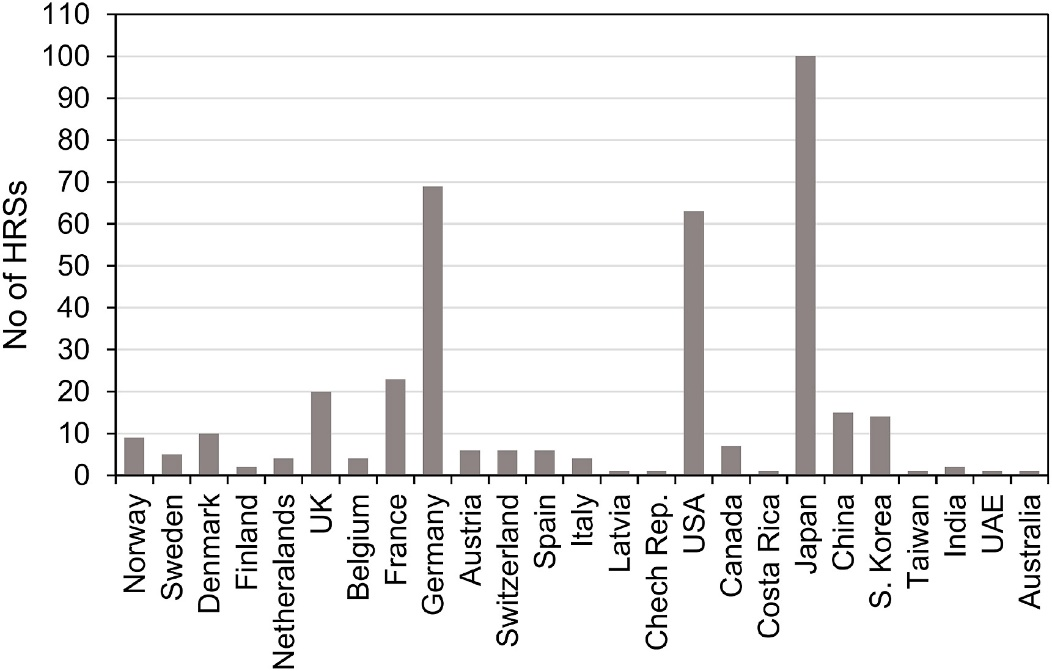
\includegraphics[width=0.6\linewidth]{image/hydrogen_refuel} \caption{Number of hydrogen refuelling stations worldwide (Apostolou and Xydis, 2019)}\label{fig:unnamed-chunk-57}
\end{figure}

The European Strategic Energy Technology Plan proposes hydrogen and fuel-cell technologies as crucial for obtaining green-house gases reduction goals by 2050 (Roadmap Europe H., 2019; Alvarez-Meaza et al., 2020). Hydrogen trucks are produced by Hyundai and Hyzon and have already been implemented in Switzerland and the Netherlands in 2021. The Xcient is the world's first mass-produced fuel cell electric truck with a range of 400 km and a charging of about 15 minutes. The American brand Hyzon Motors plans 100,000 trucks by 2030 for Europe.

\hypertarget{relevant-initiatives-in-austria-61}{%
\subsection*{Relevant initiatives in Austria}\label{relevant-initiatives-in-austria-61}}
\addcontentsline{toc}{subsection}{Relevant initiatives in Austria}

\begin{itemize}
\tightlist
\item
  \href{https://fuelcellsworks.com/news/alstoms-hydrogen-train-successfully-completes-three-months-of-testing-in-austria/\#:~:text=Alstom's\%20Hydrogen\%20Train\%20Successfully\%20Completes\%20Three\%20Months\%20of\%20Testing\%20in\%20Austria,-By\%20FuelCellsWorksDecember\&text=Alstom's\%20Coradia\%20iLint\%2C\%20the\%20world's,Austrian\%20Federal\%20Railways}{Hydrogen train}
\item
  \href{https://fuelcellsworks.com/news/the-first-hydrogen-trucks-are-rolling-in-europe/}{Hydrogen trucks}
\end{itemize}

\hypertarget{impacts-with-respect-to-sustainable-development-goals-sdgs-61}{%
\subsection*{Impacts with respect to Sustainable Development Goals (SDGs)}\label{impacts-with-respect-to-sustainable-development-goals-sdgs-61}}
\addcontentsline{toc}{subsection}{Impacts with respect to Sustainable Development Goals (SDGs)}

\begin{longtable}[]{@{}
  >{\centering\arraybackslash}p{(\columnwidth - 8\tabcolsep) * \real{0.2029}}
  >{\centering\arraybackslash}p{(\columnwidth - 8\tabcolsep) * \real{0.1884}}
  >{\centering\arraybackslash}p{(\columnwidth - 8\tabcolsep) * \real{0.2029}}
  >{\centering\arraybackslash}p{(\columnwidth - 8\tabcolsep) * \real{0.2029}}
  >{\centering\arraybackslash}p{(\columnwidth - 8\tabcolsep) * \real{0.2029}}@{}}
\toprule()
\begin{minipage}[b]{\linewidth}\centering
Impact level
\end{minipage} & \begin{minipage}[b]{\linewidth}\centering
Indicator
\end{minipage} & \begin{minipage}[b]{\linewidth}\centering
Impact direction
\end{minipage} & \begin{minipage}[b]{\linewidth}\centering
Goal description and number
\end{minipage} & \begin{minipage}[b]{\linewidth}\centering
Source
\end{minipage} \\
\midrule()
\endhead
Individual & Improved air quality & \textbf{+} & Health \& Wellbeing (\emph{3}) & Colella, Jacobson \& Golden, 2005 \\
Individual & High prices of hydrogen cars and hydrogen fuel & \textbf{-} & Equality (\emph{5,10}) & Kanna \& Paturu, 2020 \\
Individual & Cost for individuals (high acquisition costs but lower operating costs) & \textbf{\textasciitilde{}} & Sustainable economic development (\emph{8,11}) & Apostolou \& Xydis, 2019 \\
Systemic & Emissions reduced, improved air quality & \textbf{+} & Health \& Wellbeing (\emph{3}) & Colella, Jacobson \& Golden, 2005 \\
Systemic & Distribution and allocation of goods worsens & \textbf{-} & Equality (\emph{5,10}) & Kanna \& Paturu, 2020 \\
Systemic & Reduced emissions, replacement of fossil fuels, energy transition & \textbf{+} & Environmental sustainability (\emph{7,12-13,15}) & Colella, Jacobson \& Golden, 2005 \\
Systemic & Not yet profitable for manufacturers & \textbf{-} & Sustainable economic development (\emph{8,11}) & Roadmap Europe, 2019 \\
Systemic & Number of hydrogen refuelling stations increases & \textbf{+} & Innovation \& Infrastructure (\emph{9}) & Apostolou \& Xydis, 2019 \\
Systemic & Sharing technologies internationally & \textbf{+} & Partnership \& collaborations (\emph{17}) & International Partnership for Hydrogen and Fuel Cells in the Economy, n.d. \\
\bottomrule()
\end{longtable}

\hypertarget{technology-and-societal-readiness-level-61}{%
\subsection*{Technology and societal readiness level}\label{technology-and-societal-readiness-level-61}}
\addcontentsline{toc}{subsection}{Technology and societal readiness level}

\begin{longtable}[]{@{}cc@{}}
\toprule()
TRL & SRL \\
\midrule()
\endhead
7-8 & 6-8 \\
\bottomrule()
\end{longtable}

\hypertarget{open-questions-59}{%
\subsection*{Open questions}\label{open-questions-59}}
\addcontentsline{toc}{subsection}{Open questions}

\begin{enumerate}
\def\labelenumi{\arabic{enumi}.}
\tightlist
\item
  How will the hydrogen truck market evolve in the future?
\item
  How to store large amounts of energy at low weight and in a restricted space within the vehicle? (Roadmap Europe, 2019)
\end{enumerate}

\hypertarget{further-links-49}{%
\subsection*{Further links}\label{further-links-49}}
\addcontentsline{toc}{subsection}{Further links}

\begin{itemize}
\tightlist
\item
  \href{https://www.europarl.europa.eu/news/nl/press-room/20180911IPR13114/more-electric-cars-on-eu-roads-by-2030}{europarlament}
\item
  \href{https://ec.europa.eu/transport/themes/urban/vehicles/road/hydrogen_en}{ec.europa}
\item
  \href{https://www.fch.europa.eu/news/hydrogen-roadmap-europe-sustainable-pathway-european-energy-transition}{fch.europa}
\end{itemize}

\hypertarget{references-61}{%
\subsection*{References}\label{references-61}}
\addcontentsline{toc}{subsection}{References}

\begin{itemize}
\tightlist
\item
  Alvarez-Meaza, I., Zarrabeitia-Bilbao, E., Rio-Belver, R. M., \& Garechana-Anacabe, G. (2020). Fuel-Cell Electric Vehicles: Plotting a Scientific and Technological Knowledge Map. Sustainability, 12(6), 2334.
\item
  Ajanovic, A., Haas, R. (2021). Prospects and Impediments for hydrogen and fuel cell vehicles in the transport sector. International Journal of Hydrogen Energy. 46 (16), 10049-10058. \url{https://doi.org/10.1016/j.ijhydene.2020.03.122}
\item
  Apostolou, D., \& Xydis, G. (2019). A literature review on hydrogen refuelling stations and infrastructure. Current status and future prospects. Renewable and Sustainable Energy Reviews, 113(May), 109292. \url{https://doi.org/10.1016/j.rser.2019.109292}
\item
  Borgstedt, P., Neyer, B., \& Schewe, G. (2017). Paving the road to electric vehicles--A patent analysis of the automotive supply industry. Journal of cleaner production, 167, 75-87.
\item
  Colella, W. G., Jacobson, M. Z., \& Golden, D. M. (2005). Switching to a U.S. hydrogen fuel cell vehicle fleet: The resultant change in emissions, energy use, and greenhouse gases. Journal of Power Sources, 150, 150--181. \url{https://doi.org/https://doi.org/10.1016/j.jpowsour.2005.05.092}
\item
  Doppelbauer, M. (2020). Grundlagen der Elektromobilität. In Grundlagen der Elektromobilität. \url{https://doi.org/10.1007/978-3-658-29730-5}
\item
  Eichlseder, H., Klell, M., \& Trattner, A. (2018). Wasserstoff in der Fahrzeugtechnik. In Wasserstoff in der Fahrzeugtechnik. \url{https://doi.org/10.1007/978-3-8348-9674-2}
\item
  International Partnership for Hydrogen and Fuel Cells in the Economy. (n.d.). No Title. \url{https://www.iphe.net/}
\item
  Iribarren, D., Martín-Gamboa, M., Manzano, J., \& Dufour, J. (2016). Assessing the social acceptance of hydrogen for transportation in Spain: an unintentional focus on target population for a potential hydrogen economy. International journal of hydrogen energy, 41(10), 5203-5208.
\item
  Kanna, I. V., \& Paturu, P. (2020). A study of hydrogen as an alternative fuel. International Journal of Ambient Energy, 41(12), 1433--1436. \url{https://doi.org/10.1080/01430750.2018.1484803}
\item
  Lehmann, J., \& Luschtinetz, T. (2014). Wasserstoff und Brennstoffzellen.
\item
  Roadmap Europe (2019). A sustainable pathway for the European energy transition. Luxembourg: Publications Office of the European Union.
\item
  Pötscher, F., Winter, R., Lichtblau, G., Schreiber, H., \& Kutschera, U. (2014). Ökobilanz alternativer Antriebe -- Elektrofahrzeuge im Vergleich.
\item
  Schabbach, T., \& Wesselak, V. (2020). Energie - Den Erneuerbaren gehört die Zukunft.
\item
  Tanç, B., Arat, H. T., Baltacıoğlu, E., \& Kadir, A. (2019). Overview of the next quarter century vision of hydrogen fuel cell electric vehicles. In International Journal of Hydrogen Energy, Volume 44, Issue 20, (pp.~10120--10128).
\item
  Töpler, J., \& Lehmann, J. (2017). Wasserstoff und Brennstoffzelle - Technologien und Marktkonzepte. In Springer Vieweg.
\end{itemize}

\hypertarget{bev}{%
\section{Battery electric}\label{bev}}

\textbf{Updated: 20th June 2022}

\hypertarget{synonyms-56}{%
\subsection*{Synonyms}\label{synonyms-56}}
\addcontentsline{toc}{subsection}{Synonyms}

\emph{Battery electric vehicle (BEV)}

\hypertarget{definition-62}{%
\subsection*{Definition}\label{definition-62}}
\addcontentsline{toc}{subsection}{Definition}

Transport contributes up to 30\% of climate-relevant greenhouse gas emissions in Austria, with CO\textsubscript{2} playing the largest role here (Bundesministerium für Umwelt, 2019). While the average engine power of vehicles sold annually is increasing (Kreuzer, 2020), the total emissions from the transport sector are also rising (Bundesministerium für Umwelt, 2019). Without a change in mobility behaviour, only a switch to locally emission-free drive technologies, such as BEVs, can help this situation. BEVs are emission-free in operation (apart from tyre wear and minimal brake dust) and have a battery storage/accumulator installed that is charged at an external charging station. The power conversion takes place in an electric motor. The benefits and drawbacks of BEVs are presented in the table below.

\begin{longtable}[]{@{}
  >{\centering\arraybackslash}p{(\columnwidth - 2\tabcolsep) * \real{0.5000}}
  >{\centering\arraybackslash}p{(\columnwidth - 2\tabcolsep) * \real{0.5000}}@{}}
\toprule()
\begin{minipage}[b]{\linewidth}\centering
Advantages
\end{minipage} & \begin{minipage}[b]{\linewidth}\centering
Disadvantages
\end{minipage} \\
\midrule()
\endhead
\textbf{Lower noise}: Electric motors operate far more quietly than combustion engines. However, in car traffic, most noise is not generated by the engine, but by the interaction of tyres and road surface or - at high speeds - by aerodynamic noises. In these cases, there is no difference between an electric car and a conventional vehicle. It is only above about 25 kilometres per hour that rolling noises are decisive when driving a car. Below this speed, the engine noise is the determining noise source. Therefore, electric cars are quieter in low-speed areas such as residential areas or when starting at intersections and traffic lights. & \textbf{Range} currently varies from approx. 300 to 800 km, with an increasing trend over the last years. Longest ranges nowadays (2022) reach from 400 to 850 km (\href{https://www.cars.com/articles/electric-vehicles-with-the-longest-range-422227/}{Lucid Air}). The range depends on many factors, such as differences in driving style, weather conditions (it only reaches its full capacity in a temperature range between 20 and 40 degrees Celsius), air conditioning usage. Nevertheless, 94\% of all car journeys by the Austrian population are shorter than 50 km. \\
\textbf{Locally emission-free}: BEVs emit no air pollutants when in use. The reduction of greenhouse gases is strongly dependent on the energy sources with which the electricity was produced beforehand and the resulting emissions. The Austrian electricity mix already has a high proportion of renewable energy. The additional electricity demand caused by electromobility is covered many times over by the expansion plans until 2020 for electricity generation from renewable energy sources. This represents an excellent situation for electromobility in Austria. & \textbf{Electricity requirement}: With an increasing number of electric vehicles on Austrian roads, there may be varying loads on the low-voltage grid, which can lead to voltage fluctuations and interruptions. If, consequently, controlled charging is necessary in the medium to long-term, this should be included in the planning and construction of charging points. However, care must be taken to ensure that the control system corresponds to customer interests. \\
\textbf{Acquisition costs}: the cheapest electric cars cost around 20.490 euros, with a rising trend. & \textbf{System of fast charging} is cost-intensive as well as challenging in terms of safety and is particularly demanding for the electricity grid due to the high power required (\textgreater{} 20 kW per connection). Such charging stations should primarily be installed where it is compatible with the grid and where they are economical. Therefore, a cost-benefit assessment is advisable before installing fast charging stations. \\
\textbf{Charging costs}: If the electric car is charged on household electricity, the costs are just under 36 cents/kWh, at public charging stations they vary between 30-60 cents (with a rising trend over the last years). For 100 km in an e-car, electricity costs about 4.50 for charging. The corresponding costs for petrol and diesel in comparison: with a consumption of 6 litres of petrol and 5 litres of diesel respectively, currently 8.40 euros and 6.70 euros (Michael, 2020), although those numbers rose significantly at the beginning of 2022 due to the Russian-Ukrainian war (Hoffmann, 2022) & \textbf{Charging time} depends on battery capacity and charging power. At public fast charging stations, the duration is about half an hour to an hour. At a household socket 8-14 hours. \\
\textbf{Charging stations}: The number of charging stations and charging points is steadily increasing in Austria and currently stands at 9700 (E-control, 2022) publicly accessible charging points. By comparison, there are just under 2800 petrol stations in Austria (Sitte, 2019). & - \\
\bottomrule()
\end{longtable}

\hypertarget{key-stakeholders-62}{%
\subsection*{Key stakeholders}\label{key-stakeholders-62}}
\addcontentsline{toc}{subsection}{Key stakeholders}

\begin{itemize}
\tightlist
\item
  \textbf{Affected}: Conventional Cars' Drivers, Car Manufacturers, Insurers
\item
  \textbf{Responsible}: National Governments, City Government, Private Companies, International Lobbyists
\end{itemize}

\hypertarget{current-state-of-art-in-research-62}{%
\subsection*{Current state of art in research}\label{current-state-of-art-in-research-62}}
\addcontentsline{toc}{subsection}{Current state of art in research}

Research on this topic focuses mainly on technology performance, component sizing, charging stations and life cycle assessment (LCA).
LCA is a tool to assess the environmental footprint of a product, process or activity throughout its life cycle (Roy et al., 2009).
The main factors influencing the LCA of BEVs are the production of the vehicle and the provision of electricity for its operation. No direct emissions are produced during operation, but the source of electricity supply influences the amount of indirect emissions. Old batteries can be reused as stationary electricity storage units. Recycling the batteries makes it possible to use them again as a source of raw materials. The following raw materials are necessary in the production of battery electric drives: Lithium for the lithium-ion battery, cobalt also for the battery, although the demand is decreasing, and copper as a conductor material. Rare earths, particularly neodymium and dysprosium are needed for permanent magnets, but might be replaced by another motor technology in the future (Doppelbauer, 2020).

The table below compares the CO\textsubscript{2} emissions (in tonnes) during the production of cars with an internal combustion engine (ICE) and battery-powered electric vehicles (BEV), considering size of the car. The production process of BEVs, involves, compared to ICEs, 3 to 9 tonnes bigger CO\textsubscript{2} emission (Doppelbauer, 2020).

\begin{longtable}[]{@{}ccccccc@{}}
\toprule()
& & ICE & & & BEV & \\
\midrule()
\endhead
& Small & Medium & Large & Small (30 kWh) & Medium (60 kWh) & Large (90 kWh) \\
Body of the car & 2.5 & 3.8 & 5.0 & 2.5 & 3.8 & 5.0 \\
Additional components & 0.5 & 0.65 & 0.8 & 0.5 & 0.65 & 0.8 \\
HV System & - & - & - & 0.3 & 0.55 & 0.7 \\
Propulsion & 0.4 & 0.6 & 0.8 & 0.2 & 0.25 & 0.3 \\
Production & 1.5 & 1.5 & 1.5 & 1.5 & 1.5 & 1.5 \\
Battery & - & - & - & 3 & 6 & 9 \\
\textbf{Total} & \textbf{4.9} & \textbf{6.6} & \textbf{8.1} & \textbf{8} & \textbf{12.8} & \textbf{17.3} \\
\bottomrule()
\end{longtable}

This life cycle assessment considers current data on the production of battery systems for electric vehicles. Although the production of batteries requires a significant amount of energy and is therefore associated with high emissions, electric vehicles do not have components such as gearboxes and exhaust gas after-treatment and their production-related emissions.

The decisive factor for the greenhouse gas balance of vehicles is, above all, the energy used to operate the vehicle. While the use of fossil energy in petrol and diesel vehicles results in high greenhouse gas emissions, electric vehicles have no direct greenhouse gas emissions in their balance sheet. Taking into account direct and indirect emissions, the use of an electric car powered by electricity from renewable sources can save 80\% of GHG emissions compared to a fossil fuel-powered car. In addition, the use of renewable electricity also significantly reduces nitrogen oxide emissions. Particulate matter emissions, on the other hand, increase slightly, depending on the source of electricity.

The advantages of electric drives are also evident in the cumulative energy consumption, depending on the quality of the electricity. The lower specific consumption compared to fossil-fuelled vehicles should be emphasised. This is due to the high efficiency of the electric motor (Fritz et al., 2018). The negative environmental and social impacts of extracting the rare raw materials needed to produce the battery are already being reduced. The German government supports research into the economic use and recovery of raw materials and the reuse of batteries (Second Life). Batteries that require significantly less cobalt are now also available. Industry is also becoming increasingly involved in initiatives for the sustainable supply of the raw material (responsible mining) (Kurzempa, 2018).
In terms of the efficiency of this technology, the well-to-wheel efficiency in Austria calculates to 69\%. This is a significant efficiency gain as compared to a fuel cell car with an average well-to-wheel efficiency of about 27\% and a petrol-powered car at about 20\% (Bundesministerium für Umwelt Naturschutz und nukleare Sicherheit, n.d.). The losses in the electricity grid in Austria are very low and can be estimated in the range of 5\%, which results in a well-to-tank efficiency of 95\% based on 100\% green electricity.
In the course of the charging process, charging losses of 10\% occur due to resistances in the charging cable and the battery. However, an AC/DC voltage converter (rectifier) is connected upstream of the traction battery, which causes a further 5\% energy loss. In order to get the stored energy onto the road, it now flows through a DC/AC voltage converter (inverter) with 5\% energy loss and can finally be transferred to the wheel by an electric motor with 90\% efficiency. The tank-to-wheel efficiency is therefore 73\%. Gu et al., (2021) research the use of secondary use of electric vehicle battery for a closed loop supply chain perspective that proposes a model consisting of a battery (re)manufacturer, a secondary user and a government, in which the government provides and incentivises the secondary use of electric batteries. The use of different forms and ways of secondary use is currently researched under various researchers (Cui \& Ramyar et al., 2022).

\hypertarget{current-state-of-art-in-practice-62}{%
\subsection*{Current state of art in practice}\label{current-state-of-art-in-practice-62}}
\addcontentsline{toc}{subsection}{Current state of art in practice}

The number of e-cars registered worldwide has reached a new record level. At the same time, however, the growth in new registrations weakened. In 2019, around 7.9 million e-cars were registered worldwide. However, while the number of new registrations in 2018 still had a plus of 74\% compared to 2017 (1.3 million to 2.2 million), in 2019 new registrations remained almost at the same level as in 2018 with a plus of 4\% (2.3 million in 2019) (Prack, 2020).
According to the Centre for Solar Energy and Hydrogen Research Baden-Württemberg (ZSW), this development is primarily due to a reduction in e-car subsidies in China and the USA. Nevertheless, the previous year's level of new registrations was almost reached in these countries: 1,204,000 new registrations were registered in China (52,000 less), and 329,500 in the USA (31,800 less).
With around 230,000 registered vehicles, Germany is in seventh place in terms of the total number of e-cars after China, the USA, Norway, Japan, France and the UK (Prack, 2020).
But electric power is not just an alternative for personal modes of transport. Increasingly more vehicles in the commercial and public transport sectors are being electrically powered. The larger and heavier a vehicle is, the more difficult it is to electrify it due to the enormous mass of the larger batteries. However, battery technology is constantly developing, and the ranges are increasing. Even heavy semi-trailer trucks could be electrified in the near future. However, they would need batteries and overhead lines on motorways for fast charging along their routes. This is now being tested in Germany. Three routes in Hesse, Schleswig-Holstein and Baden-Württemberg are currently being equipped with overhead lines (see more in section on \protect\hyperlink{ers}{Electric Road Systems}). In many cities, such as Cologne, Berlin and Hamburg, electric buses are already part of regular service. Their electricity needs are met by fast, occasional charging at bus stops and by charging at night in depots. Many German cities plan to use all-electric buses soon (Kurzempa, 2018). Recently, the higher risk of electromobility to cause long lasting fires resulted in various electric buses being removed in cities of Germany after fires in Munich and Stuttgard (Heller, 2021; Meza, 2021).

\hypertarget{relevant-initiatives-in-austria-62}{%
\subsection*{Relevant initiatives in Austria}\label{relevant-initiatives-in-austria-62}}
\addcontentsline{toc}{subsection}{Relevant initiatives in Austria}

\begin{itemize}
\tightlist
\item
  \href{https://www.oeamtc.at/thema/elektromobilitaet/alles-ueber-elektroautos-35420295}{oeamtc.at}
\item
  \href{https://www.beoe.at/statistik/}{beoe.at}
\end{itemize}

\hypertarget{impacts-with-respect-to-sustainable-development-goals-sdgs-62}{%
\subsection*{Impacts with respect to Sustainable Development Goals (SDGs)}\label{impacts-with-respect-to-sustainable-development-goals-sdgs-62}}
\addcontentsline{toc}{subsection}{Impacts with respect to Sustainable Development Goals (SDGs)}

\begin{longtable}[]{@{}
  >{\centering\arraybackslash}p{(\columnwidth - 8\tabcolsep) * \real{0.2029}}
  >{\centering\arraybackslash}p{(\columnwidth - 8\tabcolsep) * \real{0.1884}}
  >{\centering\arraybackslash}p{(\columnwidth - 8\tabcolsep) * \real{0.2029}}
  >{\centering\arraybackslash}p{(\columnwidth - 8\tabcolsep) * \real{0.2029}}
  >{\centering\arraybackslash}p{(\columnwidth - 8\tabcolsep) * \real{0.2029}}@{}}
\toprule()
\begin{minipage}[b]{\linewidth}\centering
Impact level
\end{minipage} & \begin{minipage}[b]{\linewidth}\centering
Indicator
\end{minipage} & \begin{minipage}[b]{\linewidth}\centering
Impact direction
\end{minipage} & \begin{minipage}[b]{\linewidth}\centering
Goal description and number
\end{minipage} & \begin{minipage}[b]{\linewidth}\centering
Source
\end{minipage} \\
\midrule()
\endhead
Individual & Lower noise & \textbf{+} & Health \& Wellbeing (\emph{3}) & Bundesministerium fuer Umwelt, 2019 \\
Individual & Locally emission-free & \textbf{+} & Environmental sustainability (\emph{7,12,13,15}) & Bundesministerium fuer Umwelt, 2019 \\
Individual & Reduced travel cost & \textbf{+} & Sustainable economic development (\emph{8,11}) & Michael, 2020 \\
Systemic & Emission free but high emissions in production & \textbf{\textasciitilde{}} & Environmental sustainability (\emph{7,12,13,15}) & Fritz et al., 2018 \\
Systemic & Increasing number of charging stations & \textbf{+} & Innovation \& Infrastructure (\emph{9}) & Sitte, 2019; Kurzempa, 2018 \\
Systemic & Electric Vehicles Initiative accelerating the introduction and adoption of electric vehicles worldwide & \textbf{+} & Partnership \& collaborations (\emph{17}) & IEA, 2020 \\
\bottomrule()
\end{longtable}

\hypertarget{technology-and-societal-readiness-level-62}{%
\subsection*{Technology and societal readiness level}\label{technology-and-societal-readiness-level-62}}
\addcontentsline{toc}{subsection}{Technology and societal readiness level}

\begin{longtable}[]{@{}cc@{}}
\toprule()
TRL & SRL \\
\midrule()
\endhead
8-9 & 7-9 \\
\bottomrule()
\end{longtable}

\hypertarget{open-questions-60}{%
\subsection*{Open questions}\label{open-questions-60}}
\addcontentsline{toc}{subsection}{Open questions}

\begin{enumerate}
\def\labelenumi{\arabic{enumi}.}
\tightlist
\item
  How can supply bottlenecks along the value creation chain be addressed?
\item
  What is the potential shift in dependency from oil-producing to lithium producing countries? What is the expected timeframe?
\item
  How can secondary use of vehicle batteries be incentivised and fostered in the future?
\item
  How can local governments increase consumer awareness about BEVs?
\end{enumerate}

\hypertarget{further-links-50}{%
\subsection*{Further links}\label{further-links-50}}
\addcontentsline{toc}{subsection}{Further links}

\begin{itemize}
\tightlist
\item
  \href{https://www.bmu.de/fileadmin/Daten_BMU/Pools/Broschueren/elektromobilitaet_broschuere_en_bf.pdf}{bmu.de}
\item
  \href{https://publik.tuwien.ac.at/files/publik_272020.pdf}{publik.tuwien.ac.at}
\item
  \href{https://www.isi.fraunhofer.de/content/dam/isi/dokumente/cct/2020/Fact_check_Batteries_for_electric_cars.pdf}{isi.fraunhofer.de}
\item
  \href{https://www.kleinezeitung.at/auto/elektroauto/5479610/Jaenner-bis-Dezember-2020_Das-sind-die-meistverkauften\#image-01_Volkswagen-e-Golf-2017-1600-01_1534157268197687_v0_h}{kleinezeitung.at}
\item
  \href{https://www.volkswagen.at/elektroauto/id-magazin/mobilitaet/elektromobilitaet-europa}{volkswagen.at}
\item
  \href{https://www.adac.de/rund-ums-fahrzeug/elektromobilitaet/kaufen/elektroautos-uebersicht/}{adac.de}
\item
  \href{https://ec.europa.eu/eurostat/databrowser/view/ROAD_EQR_CARPDA__custom_91702/bookmark/table?lang=de\&bookmarkId=7e47ef9d-b80b-4bd6-a35b-046cb5af4500}{ec.europa.eu}
\end{itemize}

\hypertarget{references-62}{%
\subsection*{References}\label{references-62}}
\addcontentsline{toc}{subsection}{References}

\begin{itemize}
\tightlist
\item
  Bundesministerium für Umwelt, N. und nukleare S. (BMU). (2019). Wie umweltfreundlich sind Elektroautos? 1--20. www.bmu.de
\item
  Bundesministerium für Umwelt Naturschutz und nukleare Sicherheit. (n.d.). Effizienz und Kosten: Lohnt sich der Betrieb eines Elektroautos? \textbar{} BMU. Available at: \url{https://www.bmu.de/themen/luft-laerm-verkehr/verkehr/elektromobilitaet/effizienz-und-kosten/} {[}Accessed: 19 February 2021{]}
\item
  Cui, X., Ramyar, A., Siegel, J., Mohtat, P., Stefanopoulou, A. G., Avestruz, T. (2022). Comparing power processing system approaches in second-use battery energy buffering for electric vehicle charging. Journal of Energy Storage. 49, 104017. \url{https://doi.org/10.1016/j.est.2022.104017}
\item
  Doppelbauer, M. (2020). Grundlagen der Elektromobilität. In Grundlagen der Elektromobilität. \url{https://doi.org/10.1007/978-3-658-29730-5}
\item
  Eichlseder, H., Klell, M., \& Trattner, A. (2018). Wasserstoff in der Fahrzeugtechnik. In Wasserstoff in der Fahrzeugtechnik. \url{https://doi.org/10.1007/978-3-8348-9674-2}
\item
  E-Control (2022). Quartalsbericht zum Ladestellenverzeichnis (Q3 2021). \url{https://www.e-control.at/documents/1785851/1811582/102021-quartalsbericht-ladestellenverzeichnis-q3-2021-03.pdf/208c4680-3c8b-e1af-ad00-f241e1869f1c?t=1636036556717} {[}Accessed: 16 June 2022{]}
\item
  Fritz, D., Heinfellner, H., Lichtblau, G., Pölz, W., \& Stranner, G. (2018). Update: Ökobilanz alternativer Antriebe. 1--16. \url{https://umweltbundesamt.at/fileadmin/site/publikationen/DP152.pdf}
\item
  Gu, X., Zhou, L., Huang, H., Shi, X., Ieromonachou, P. (2021). Electric vehicle battery secondary use under government subsidy: A closed-loop supply chain perspective. International Journal of Production Economics. 234, 108035. \url{https://doi.org/10.1016/j.ijpe.2021.108035}
\item
  Heller, M. (2021). Elektrobus löste Großbrand aus -- München zieht E-Fahrzeuge aus dem Verkehr. \url{https://www.welt.de/vermischtes/article234310454/Elektrobus-loeste-Grossbrand-aus-Muenchen-zieht-E-Fahrzeuge-aus-dem-Verkehr.html?icid=search.product.onsitesearch} {[}Accessed: 18 June 2022{]}
\item
  Hoffmann, N. (2022). Forbes: 3 Gründe, warum die Heizölpreise 2022 steigen. \url{https://www.forbes.com/advisor/de/oel/heizoelpreise/} {[}Accessed: 17 June 2022{]}
\item
  IEA. (2020, October 26). Electric Vehicles Initiative -- Programmes and partnerships - IEA. \url{https://www.iea.org/areas-of-work/programmes-and-partnerships/electric-vehicles-initiative}
\item
  Kreuzer, C. (2020, September 8). Österreicher fahren auf immer PS-stärkere Autos ab \textbar{} Wiener Städtische. \url{https://www.wienerstaedtische.at/unternehmen/presse/pressemeldungen/detail/oesterreicher-fahren-auf-immer-ps-staerkere-autos-ab.html}
\item
  Kurzempa, A. (2018). Electromobility -- what does it mean? AUTOBUSY -- Technika, Eksploatacja, Systemy Transportowe, 19(6), 894--897. \url{https://doi.org/10.24136/atest.2018.197}
\item
  Lehmann, J., \& Luschtinetz, T. (2014). Wasserstoff und Brennstoffzellen.
\item
  Michael. (2020, January 26). Wasserstoff, E-Auto, E-Fuels: Warum das E-Auto die beste Alternative ist \textbar{} Elektroauto-News.net. \url{https://www.elektroauto-news.net/2020/wasserstoff-e-auto-e-fuels-batterieauto-beste-alternative}
\item
  Meza, E. (2021). Several German cities halt use of e-buses following series of unresolved cases of fire. \url{https://www.cleanenergywire.org/news/several-german-cities-halt-use-e-buses-following-series-unresolved-cases-fire} {[}Accessed: 18 June 2022{]}
\item
  Pötscher, F., Winter, R., Lichtblau, G., Schreiber, H., \& Kutschera, U. (2014). Ökobilanz alternativer Antriebe -- Elektrofahrzeuge im Vergleich.
\item
  Prack, N. (2020, February 27). Anzahl der Elektroautos: Deutschland \& Ausland \textbar{} ADAC. \url{https://www.adac.de/news/statistik-e-autos/}
\item
  Roy, P., Nei, D., Orikasa, T., Xu, Q., Okadome, H., Nakamura, N., \& Shiina, T. (2009). A review of life cycle assessment (LCA) on some food products. Journal of Food Engineering, 90(1), 1--10. \url{https://doi.org/https://doi.org/10.1016/j.jfoodeng.2008.06.016}
\item
  Schabbach, T., \& Wesselak, V. (2020). Energie - Den Erneuerbaren gehört die Zukunft.
\item
  Sitte, P. (2019, January 21). E-Mobilität: Zahl der Ladestationen für Elektroautos steigt weiter an \textbar{} Bundesverband Elektromobilität Österreich (BEÖ), 21.01.2019. \url{https://www.ots.at/presseaussendung/OTS_20190121_OTS0048/e-mobilitaet-zahl-der-ladestationen-fuer-elektroautos-steigt-weiter-an-bild}
\item
  Statistik Austria (2022). Kraftfahrzeuge -- Bestand. \url{http://www.statistik.at/web_de/statistiken/energie_umwelt_innovation_mobilitaet/verkehr/strasse/kraftfahrzeuge_-_bestand/index.html} {[}Accessed: 17 June 2022{]}
\item
  Töpler, J., \& Lehmann, J. (2017). Wasserstoff und Brennstoffzelle - Technologien und Marktkonzepte. In Springer Vieweg.
\end{itemize}

\hypertarget{plugin_hybrid}{%
\section{Plugin hybrid vehicles}\label{plugin_hybrid}}

\textbf{Updated: 20th June 2022}

\hypertarget{synonyms-57}{%
\subsection*{Synonyms}\label{synonyms-57}}
\addcontentsline{toc}{subsection}{Synonyms}

\emph{Hybrid, HEV, PHEV}

\hypertarget{definition-63}{%
\subsection*{Definition}\label{definition-63}}
\addcontentsline{toc}{subsection}{Definition}

Plug-in hybrid vehicles effectively combine the electric drive with either a conventional combustion engine or other engines that use alternative fuels. This has the advantage that the vehicles can travel long distances, but consumption and emissions are reduced. An energy management system ensures that the optimum amount of energy is drawn from the two energy sources while driving. The ratio of energy consumption is influenced by the driving cycle. The faster the vehicle drives, the more energy is needed (Aswin and Senthilmurugan, 2018).

A hybrid vehicle is superior in terms of the reduced carbon footprint, better mileage than conventional vehicles, financial assistance for purchase, lower annual cost and a regenerative braking system. At the same time, the disadvantages include high purchasing cost, lower fuel efficiency because the extra parts installed take up more space and add weight, and higher maintenance costs due to the dual engine. Additionally, some concerns have been risen about the risk that the battery may explode in the event of an accident (Aswin and Senthilmurugan, 2018).

However, the safety aspect referred to above can be neglected, as the results in the EuroNCAP crash test show that hybrid vehicles are just as safe as vehicles with conventional drive systems. Toyota's Hybrid Synergy Drive technology (HSD) also serves as an example, where Toyota's hybrid system - based on the airbag trigger signal - immediately switches off all electrical systems in the event of an accident and interrupts the battery contact (ADAC, 2019).

Currently, there are several types of hybrid vehicles available on the market:

\begin{itemize}
\tightlist
\item
  Series hybrid
\end{itemize}

The series hybrid model consists of an internal combustion engine that drives a generator instead of driving the wheels directly. The wheels of the car get their power from the electric motors. The generator powers both the charging battery and the wheels of the car. Series hybrids generate the maximum energy at the time of acceleration and return the energy at the time of regenerative braking. The electric vehicles are designed in such a way that a motor is connected to each wheel. The combination of motor and wheel has the disadvantage of increasing mass and thus affecting handling, but the advantage of improved traction control.

\begin{itemize}
\tightlist
\item
  Parallel hybrid
\end{itemize}

The parallel hybrid vehicle is an integration of an electric motor and an internal combustion engine connected in parallel to the mechanical transmission. The parallel hybrid architecture incorporates both the engine and the electric generator into one unit located between the transmission and the combustion engine. The battery is recharged by regenerative braking. There is a mechanical coupling between the engine and the wheel, recharging the battery cannot occur when the car is moving.

\begin{itemize}
\tightlist
\item
  Combine hybrid
\end{itemize}

The combined hybrid vehicle is a fusion of parallel and series hybrid (series-parallel hybrid). There is a double connection (electrical and mechanical) between the drive axle and the engine. The power transmission to the wheels can be either electric or mechanical. At low speeds it behaves like a series hybrid electric vehicle, but at higher speeds series drive trains are less likely to be preferred and the vehicle motor takes over. This model is significantly more expensive than parallel models as they require a mechanically split drive system, an additional generator and high computing power for dual control (Aswin and Senthilmurugan, 2018).

\hypertarget{key-stakeholders-63}{%
\subsection*{Key stakeholders}\label{key-stakeholders-63}}
\addcontentsline{toc}{subsection}{Key stakeholders}

\begin{itemize}
\tightlist
\item
  \textbf{Affected}: Conventional Cars' Drivers
\item
  \textbf{Responsible}: National Governments, Car Manufacturers, International lobbyists, Private Companies
\end{itemize}

\hypertarget{current-state-of-art-in-research-63}{%
\subsection*{Current state of art in research}\label{current-state-of-art-in-research-63}}
\addcontentsline{toc}{subsection}{Current state of art in research}

Current research efforts focus on the reduction of battery size while maintaining the electric driving performance. Therefore, the study by Song et al.~(2018) suggest 30.4 kWh as an optimal battery capacity. Another, large research developments are performed with respect to reduction of emissions and continuous testing of environmental efficiency in comparison to conventional cars. In an ADAC test of plug-in hybrids, just two cars scored well in the Ecotest, namely Hyundai Ioniq and Volvo V60. The Hyundai was very energy-efficient, while the Volvo consumed more energy and emitted more carbon dioxide, but its exhaust gases were cleaner. This allowed it to score well in terms of pollutants. However, the test results leave no doubt that large and heavy cars like the BMW X5 and Mercedes GLE, even as plug-in hybrids, consume a lot of energy and therefore cannot be counted as eco-mobiles (Kroher, 2020). Interestingly, recent test conducted on the newest models of PHEV showed that they pollute the environment two to four times more than the manufacturers claim which undermined the public opinion on the environmental advantages offered by the PHEV (Plötz et al., 2020; Bannon, 2020).

\hypertarget{current-state-of-art-in-practice-63}{%
\subsection*{Current state of art in practice}\label{current-state-of-art-in-practice-63}}
\addcontentsline{toc}{subsection}{Current state of art in practice}

The development of the hybrid electric vehicle is evolving into the next generation of the mode of transport, in line with EU's policy aims of reduction of greenhouse gas emissions. Nevertheless, current market penetration is still relatively low, contributing to 1\% of total car registrations (as of 2019). In Europe, the leaders in the uptake of plug-in hybrid vehicles are Finland and Sweden followed by the United Kingdom (European Environment Agency, 2020).

In Austria the number of plug-in hybrid vehicles quadrupled in 2020 from January to October compared to the same period last year. By the end of October, about 5,500 new vehicles of this type had been registered. Of the approximately 14,700 applications for e-car subsidies so far this year, 90 percent are purely electric, ten percent are plug-in hybrids and range extenders (Ortner, 2020).
The results of a study by the Frauenhofer Institute show that the actual climate balance of plug-in hybrid passenger cars is poor, the real CO\textsubscript{2} emissions are twice as high as the values determined in the test cycle, for company cars the real CO\textsubscript{2} emissions are even three to four times as high. The VCÖ calls for a rapid change in the subsidies for plug-in hybrid cars in Austria (VCÖ, 2020).

By 2020, there are already 800 public e-charging points in Vienna, with number close to a thousand, Vienna is one of the leading e-mobility cities in Europe (Fischer, 2020). The Austrian energy companies - members of the BEÖ - have driven the expansion of the public charging infrastructure in recent years. With over 5,000 charging points between Vienna and Bregenz, Austria provides one of the densest charging networks in Europe (Sitte, 2020b).By the end of 2021 the number of charging points in Austria rose to 9,700 (E-Control, 2022) an 85.850 licensed EVs (Statistik Austria, 2022) which results in about 1 charging station for 8 electric cars. Consequently, charging stations at the place of residence are indispensable for a quick and convenient charging option. Until end of 2021, all building owners had to agree to the installation of an e-charging station. This unanimity made it complicated, to install e-charging stations in apartment buildings, which is needed for a quick and convenient charging option. With the beginning of 2022 and the released ``WEG-Novelle 2022'' (Condominium Amendment Act), which is intended to serve the achievement of the internationally specified climate targets, this unanimity was changed in the area of the ``consent fiction'', which makes it possible that henceforth not the majority of the apartment owners is required, but the majority of the persons responding to the request vote for these structural measures. Further details on the amendment of the condominium act in Austria can be extracted \href{https://iura.at/PDF/Kanzleinachrichten/Fully\%20Loaded\%20-\%20Beitrag\%20zur\%20WEG-Novelle\%202022_18.02.2022.pdf}{here}.

\hypertarget{relevant-initiatives-in-austria-63}{%
\subsection*{Relevant initiatives in Austria}\label{relevant-initiatives-in-austria-63}}
\addcontentsline{toc}{subsection}{Relevant initiatives in Austria}

\begin{itemize}
\tightlist
\item
  \href{https://www.oesterreich.gv.at/themen/bauen_wohnen_und_umwelt/elektroautos_und_e_mobilitaet/Seite.4320010.html}{oesterreich.gv}
\item
  \href{https://www.vcoe.at/presse/presseaussendungen/detail/vcoe-neue-studie-zeigt-schlechte-klimabilanz-von-plug-in-hybrid-pkw}{vcoe.at}
\item
  \href{https://www.ladestellen.at/\#/electric}{ladestellen.at}
\end{itemize}

\hypertarget{impacts-with-respect-to-sustainable-development-goals-sdgs-63}{%
\subsection*{Impacts with respect to Sustainable Development Goals (SDGs)}\label{impacts-with-respect-to-sustainable-development-goals-sdgs-63}}
\addcontentsline{toc}{subsection}{Impacts with respect to Sustainable Development Goals (SDGs)}

\begin{longtable}[]{@{}
  >{\centering\arraybackslash}p{(\columnwidth - 8\tabcolsep) * \real{0.2029}}
  >{\centering\arraybackslash}p{(\columnwidth - 8\tabcolsep) * \real{0.1884}}
  >{\centering\arraybackslash}p{(\columnwidth - 8\tabcolsep) * \real{0.2029}}
  >{\centering\arraybackslash}p{(\columnwidth - 8\tabcolsep) * \real{0.2029}}
  >{\centering\arraybackslash}p{(\columnwidth - 8\tabcolsep) * \real{0.2029}}@{}}
\toprule()
\begin{minipage}[b]{\linewidth}\centering
Impact level
\end{minipage} & \begin{minipage}[b]{\linewidth}\centering
Indicator
\end{minipage} & \begin{minipage}[b]{\linewidth}\centering
Impact direction
\end{minipage} & \begin{minipage}[b]{\linewidth}\centering
Goal description and number
\end{minipage} & \begin{minipage}[b]{\linewidth}\centering
Source
\end{minipage} \\
\midrule()
\endhead
Individual & Carbon dioxide emissions reduced & \textbf{+} & Health \& Wellbeing (\emph{3}) & Koellner, 2020 \\
Individual & Number of e-charging points increases & \textbf{+} & Innovation \& Infrastructure (\emph{9}) & Sitte, 2020a \\
Systemic & Emissions reduced for small and light vehicles only & \textbf{\textasciitilde{}} & Environmental sustainability (\emph{7,12-13,15}) & Kroher, 2020; VCOE, 2020 \\
Systemic & Exhaust gas treatment strategies are developed & \textbf{+} & Innovation \& Infrastructure (\emph{9}) & Schaefer, 2020 \\
\bottomrule()
\end{longtable}

\hypertarget{technology-and-societal-readiness-level-63}{%
\subsection*{Technology and societal readiness level}\label{technology-and-societal-readiness-level-63}}
\addcontentsline{toc}{subsection}{Technology and societal readiness level}

\begin{longtable}[]{@{}cc@{}}
\toprule()
TRL & SRL \\
\midrule()
\endhead
8-9 & 7-9 \\
\bottomrule()
\end{longtable}

\hypertarget{open-questions-61}{%
\subsection*{Open questions}\label{open-questions-61}}
\addcontentsline{toc}{subsection}{Open questions}

\begin{enumerate}
\def\labelenumi{\arabic{enumi}.}
\tightlist
\item
  How the increased use of PHEV will influence the market of second-hand cars?
\item
  What is the impact of batteries on the life cycle of the car?
\end{enumerate}

\hypertarget{further-links-51}{%
\subsection*{Further links}\label{further-links-51}}
\addcontentsline{toc}{subsection}{Further links}

\begin{itemize}
\tightlist
\item
  \href{https://www.tagesschau.de/wirtschaft/technologie/methanol-brennstoffzelle-antrieb-auto-101.html}{Tagesschau.de}
\item
  \href{https://www.europarl.europa.eu/news/nl/press-room/20180911IPR13114/more-electric-cars-on-eu-roads-by-2030}{Europarlament}
\item
  \href{https://ec.europa.eu/transport/themes/urban/vehicles/road/hydrogen_en}{Ec.europa}
\item
  \href{https://www.fch.europa.eu/news/hydrogen-roadmap-europe-sustainable-pathway-european-energy-transition}{Fch.europa}
\end{itemize}

\hypertarget{references-63}{%
\subsection*{References}\label{references-63}}
\addcontentsline{toc}{subsection}{References}

\begin{itemize}
\tightlist
\item
  ADAC. (2019). Hybridantrieb: Funktionsweise sowie Vor- und Nachteile. \url{https://www.adac.de/verkehr/tanken-kraftstoff-antrieb/alternative-antriebe/hybridantrieb/}
\item
  Aswin, A., \& Senthilmurugan, S. (2018). A survey on power levels of battery charging and infrastructure for plug-in electric and hybrid vehicles. IOP Conference Series: Materials Science and Engineering, 402(1). \url{https://doi.org/10.1088/1757-899X/402/1/012154}
\item
  Bannon, E., (2020). Plug-In Hybrids In New Emissions Scandal As Tests Show Higher Pollution Than Claimed \textbar{} Transport \& Environment. Transportenvironment.org. Available at: \url{https://www.transportenvironment.org/press/plug-hybrids-new-emissions-scandal-tests-show-higher-pollution-claimed} {[}Accessed: 19 January 2021{]}.
\item
  European Environment Agency. (2020). INDICATOR ASSESSMENT New Registrations Of Electric Vehicles In Europe. Available at: \url{https://www.eea.europa.eu/data-and-maps/indicators/proportion-of-vehicle-fleet-meeting-5/assessment} {[}Accessed: 19 January 2021{]}
\item
  Fischer, S. M. (2020, September 2). Ökostrom an jeder Ecke: Ladestellen-Ausbau auf Zielgeraden \textbar{} Wien Energie GmbH, 02.09.2020. \url{https://www.ots.at/presseaussendung/OTS_20200902_OTS0138/oekostrom-an-jeder-ecke-ladestellen-ausbau-auf-zielgeraden}
\item
  Köllner, C. (2020). Das sollten Sie über Plug-in-Hybride wissen. \url{https://www.springerprofessional.de/plug-in-hybrid/antriebsstrang/das-sollten-sie-ueber-plug-in-hybride-wissen/18235362}
\item
  Kroher, T. (2020). Plug-in-Hybrid: Modelle, Verbrauch, Technik, Kosten, Ökobilanz. \url{https://www.adac.de/rund-ums-fahrzeug/autokatalog/marken-modelle/auto/plug-in-hybrid/}
\item
  Ortner, M. (2020, December 9). Plug-in-Hybride sind nur so umweltfreundlich wie ihre Fahrer - Wiener Zeitung Online. \url{https://www.wienerzeitung.at/nachrichten/wirtschaft/oesterreich/2084730-Plug-In-Hybride-nur-so-umweltfreundlich-wie-ihre-Fahrer.html}
\item
  Plötz, P., Moll, C., Biecker, G., Mock, P., \& Li, Y. (2020). Real-World Usage of Plug-in Hybrid Electric Vehicles: Fuel Consumption, Electric Driving, and CO₂ Emissions.
\item
  Schäfer, P. (2020). Empa errechnet beste Kaltstart-Strategie für Hybridfahrzeuge. \url{https://www.springerprofessional.de/hybridtechnik/abgasnachbehandlung/empa-errechnet-beste-kaltstart-strategie-fuer-hybridfahrzeuge/17751190}
\item
  Sitte, P. (2020a, June 29). BEÖ begrüßt E-Mobilitätsförderung 2020 \textbar{} Bundesverband Elektromobilität Österreich (BEÖ), 29.06.2020. \url{https://www.ots.at/presseaussendung/OTS_20200629_OTS0144/beoe-begruesst-e-mobilitaetsfoerderung-2020}
\item
  Sitte, P. (2020b, July 15). BEÖ: Strom laden in eigener Garage wird einfacher. Wichtiger Schritt für E-Mobilität. \textbar{} Bundesverband Elektromobilität Österreich (BEÖ), 15.07.2020. \url{https://www.ots.at/presseaussendung/OTS_20200715_OTS0148/beoe-strom-laden-in-eigener-garage-wird-einfacher-wichtiger-schritt-fuer-e-mobilitaet}
\item
  Song, Z., Zhang, X., Li, J., Hofmann, H., Ouyang, M., \& Du, J. (2018). Component sizing optimization of plug-in hybrid electric vehicles with the hybrid energy storage system. Energy, 144, 393--403. \url{https://doi.org/10.1016/j.energy.2017.12.009}
\item
  VCÖ. (2020). VCÖ: Neue Studie zeigt schlechte Klimabilanz von Plug-In-Hybrid Pkw - Mobilität mit Zukunft. \url{https://www.vcoe.at/presse/presseaussendungen/detail/vcoe-neue-studie-zeigt-schlechte-klimabilanz-von-plug-in-hybrid-pkw}
\end{itemize}

\hypertarget{reference}{%
\chapter{References}\label{reference}}

\begin{itemize}
\tightlist
\item
  Lovelace, R., Nowosad, J., Muenchow J. (2021) \emph{Geocomputation with R.} \url{https://geocompr.robinlovelace.net/}
\item
  Afrimap team. \emph{Afrimapr book.} \url{https://github.com/afrimapr/afrimapr-book}
\item
  Xie, Y. (2015). \emph{Dynamic Documents with R and Knitr.} 2nd ed.~Boca Raton, Florida: Chapman; Hall/CRC. \url{http://yihui.org/knitr/}.
\item
  Xie, Y. (2021). \emph{bookdown: Authoring Books and Technical Documents with R Markdown.} \url{https://bookdown.org/yihui/bookdown/}
\end{itemize}

  \bibliography{book.bib,packages.bib}

\end{document}
